% This file makes a web version of the blueprint
% It should include all the \usepackage needed for this version.
% The template includes standard AMS packages.
% It is otherwise a very minimal preamble (you should probably at least
% add cleveref and tikz-cd).

\documentclass{report}

\usepackage{amssymb, amsthm, amsmath}
\usepackage{hyperref}
\usepackage{graphicx}
\graphicspath{{figures/}}
\usepackage{tikz}
\usetikzlibrary{positioning, arrows.meta, calc, fit}
\usepackage{pgfplots}
\pgfplotsset{compat=1.16}
% tpl: repo-local copy of plastexdepgraph's dep_graph.html that restructures
% the dot source before rendering: one cluster per chapter, stacked in chapter
% order; a dependency on another chapter's statement drawn as a dashed portal
% node inside the chapter that uses it (no edge crosses a chapter); the base
% definitions every chapter uses (pdiv, hasvjp) drawn once. The \uses lines the
% graph is drawn from are generated — scripts/blueprint_uses.py.
\usepackage[showmore, dep_graph, tpl=templates/dep_graph.html]{blueprint}


% In this file you should put all LaTeX macros and settings to be used both by
% the pdf version and the web version.
% This should be most of your macros.

% The theorem-like environments defined below are those that appear by default
% in the dependency graph. See the README of leanblueprint if you need help to
% customize this. 
% The configuration below use the theorem counter for all those environments
% (this is what the [theorem] arguments mean) and never resets it.
% If you want for instance to number them within chapters then you can add
% [chapter] at the end of the next line.
\newtheorem{theorem}{Theorem}
\newtheorem{proposition}[theorem]{Proposition}
\newtheorem{lemma}[theorem]{Lemma}
\newtheorem{corollary}[theorem]{Corollary}

\theoremstyle{definition}
\newtheorem{definition}[theorem]{Definition}

% Custom "axiom" environment for primitives we axiomatize rather than prove.
% We reuse the `proposition` counter so it shows up on the dep graph.
\newtheorem{axiom}[theorem]{Axiom}

% Math notation used throughout
\newcommand{\R}{\mathbb{R}}
\newcommand{\Vect}[1]{\mathbb{R}^{#1}}
\newcommand{\Mat}[2]{\mathbb{R}^{#1 \times #2}}
\newcommand{\pdiv}{\operatorname{pdiv}}
\newcommand{\pdivMat}{\operatorname{pdivMat}}
\newcommand{\HasVJP}{\mathsf{HasVJP}}
\newcommand{\HasVJPMat}{\mathsf{HasVJPMat}}
\newcommand{\HasVJPthree}{\mathsf{HasVJP3}}
% Foundation-flip notation (post the axiom-elimination work).
\newcommand{\fderiv}{\operatorname{fderiv}}
\newcommand{\basisVec}{\mathbf{e}}
\newcommand{\Differentiable}{\mathsf{Differentiable}}
\newcommand{\vjp}{\operatorname{vjp}}
\newcommand{\vjpMat}{\operatorname{vjpMat}}
\newcommand{\biPathMat}{\operatorname{biPathMat}}
\newcommand{\bnIstdBroadcast}{\operatorname{bnIstdBroadcast}}

% Lamport-style structured proofs ("How to Write a 21st Century Proof").
% \Assume/\Prove head a theorem statement; inside a proof, each enumerated
% step carries its own justification via \pf{...}. \Suffices restates the
% goal, \Case opens a case of an exhaustive split, \Qed is the mandatory
% final step (named \Qed because unicode-math claims \QED for U+220E at
% \begin{document}). \prev is Lamport's "@": the expression established
% by the preceding step.
\newcommand{\Assume}{\textsc{assume:}}
\newcommand{\Prove}{\textsc{prove:}}
\newcommand{\pf}[1]{\\ \textsc{proof:} #1}
\newcommand{\Suffices}{\textsc{suffices:}}
\newcommand{\Case}{\textsc{case}}
\newcommand{\Qed}{\textsc{q.e.d.}}
\newcommand{\prev}{\mathord{@}}

% Base URL for doc-gen4 output. Change this one line to repoint all
% \leandocref{...} hyperlinks (e.g. file:// for local preview, staging URL).
\newcommand{\docbase}{https://brettkoonce.github.io/lean4-mlir/docs}
% In this file you should put macros to be used only by
% the web version. Of course they should have a corresponding
% version in macros/print.tex.
% Typically the printed version could have more fancy decorations.
% This will probably be a very short file.

% Inline doc-gen4 cross-reference for the web build. Renders
% \leandocref{Proofs.pdiv\_comp} as a clickable typewriter link to the
% corresponding declaration's API doc page.
\newcommand{\leandocref}[1]{\href{\docbase/find/\#doc/#1}{\texttt{#1}}}

% \prosesection: chapter-body prose sub-heading. Rendered as a styled bold
% heading that is NOT a sectioning command, so it never produces a web
% sidebar entry -- the ch1-9 web index then shows only numbered sections,
% matching the PDF TOC. The printed version (macros/print.tex) keeps it as
% a normal \section*.
\newcommand{\prosesection}[1]{\par\bigskip\noindent{\large\bfseries #1}\par\nopagebreak\smallskip}


\home{https://lean.brettkoonce.com}
\github{https://github.com/brettkoonce/lean4-mlir}
\dochome{https://lean.brettkoonce.com/docs}

% Web title is the bare main title only — the subtitle (kept on the print
% title page) costs too much vertical space on mobile at the top of the page.
\title{Verified Deep Learning with Lean 4}
\author{Brett Koonce}

\begin{document}
\maketitle
% Blueprint for the Verified VJP Proofs suite (LeanMlir/Proofs/)
%
% Every axiom, definition, and theorem in the suite is annotated below so
% leanblueprint can render the dependency graph. Each block cites its
% Lean declaration via \lean{...}, marks proved claims with \leanok, and
% lists upstream dependencies via \uses{...}.

% Standard lead-in before every ImageNet recipe section: ImageNet runs on
% the phase-2 (Lean->JAX) trainer to validate the framework's logic; phase-3
% verified-IREE codegen led to phase 4 (PJRT), the eventual destination.
\newcommand{\imagenetphasenote}{\emph{Why the phase-2 trainer?} The
ImageNet numbers in this book come from the phase-2 (Lean$\to$JAX) trainer: at
this scale its job is to validate the framework's logic end to end, and it is
the reference the verified path is measured against. Phase-3 verified-IREE
codegen led to phase 4 --- PJRT, which is the verified path itself. Where a
section has both, it reports both.}

% The companion marker on every worked example: these run on phase-3
% verified-IREE codegen. Between this and \imagenetphasenote, every demo in
% the book states its execution path -- i.e. the set of them is the map of
% what phase 4 still has to absorb.
\newcommand{\phasethreenote}{\emph{Which trainer is this?} This demo runs
on the phase-3 verified-IREE path --- the proven graph, compiled by IREE
and executed on the GPU --- which is what the numbers below were measured
on. It has a phase-4 (PJRT) peer already built, and phase 4 is where it is
headed.}

% ─── Re-run status of ImageNet result tables ──────────────────────────────────
% Three changes landed 2026-08-04..08-14 that make older ImageNet numbers
% incomparable: timm's validation protocol + antialiased resampler, the 50,000-image
% denominator, and a strided-conv padding fix that changed the emitted NETWORK — so
% an old checkpoint cannot be re-scored either, it would run in a network it was
% never trained in.
%
% \imagenettimmnote is an EXCEPTION MARKER, not a status field: a section carries it
% only while its numbers still predate the change. A re-run section carries nothing —
% current numbers are the default the reader should assume, and a banner on every
% table announcing it would be noise.
%
% Chapter 5 (ResNet-34 / ResNet-50) is the worked example of a chapter already rolled
% over. Doing the next one is three mechanical steps: re-run it, DELETE its
% \imagenettimmnote, and replace any row you are NOT re-running with \withheld so the
% table shows --- rather than a stale figure that reads as current.
\newcommand{\imagenettimmnote}{\textbf{[TODO: run with timm tweaks.]} The
numbers in this section were measured before the trainers moved onto
\texttt{timm}'s validation protocol and its antialiased resampler
(appendix~\ref{app:data}). That change moves the training distribution as
well as the evaluation, so it needs a re-run rather than a re-score, and
none of it is reflected below.}

% One result cell whose figure predates the re-run and is withheld rather than
% quoted. The row stays — its throughput columns are still valid — and the gap is
% the honest statement that nobody has measured this yet under the current rules.
\newcommand{\withheld}{---}

\chapter*{Introduction}
\addcontentsline{toc}{chapter}{Introduction}
\label{chap:introduction}

On the next-to-last page of my first book, I wrote that I dreamed of a
future where we could take our code and compile it for whatever backend
we desire, via MLIR. I meant it as a wishlist item, something I expected
to happen eventually but not soon enough to matter for that work.

It turned out ``eventually'' was about five years.

This is the book I wanted to write back then and couldn't. The tools
weren't ready. Lean 4 was still in development, MLIR was a research
project, and driving a GPU still meant going through Python. All three
are production-quality now, and the thing I wished for is sitting in a
GitHub repo, training ResNets on a single GPU, with machine-checked proofs that
every gradient is correct.

\section*{What this book is about}

This book teaches you how backpropagation actually works.

You already know the hand-wave version. Compute gradients, update
weights, repeat. If you've trained a model you've called
\texttt{.backward()} a thousand times, but what you probably haven't done
is open the hood, look at what \texttt{.backward()} is actually
computing layer by layer, and verify that the computation is
mathematically correct.

That's what we're going to do. We'll take every layer in the modern
stack: dense, ReLU, convolution, pooling, batch normalization, residual
connections, depthwise convolution, squeeze-and-excitation, layer
normalization, and self-attention. For each one we will:

\begin{enumerate}
  \item \textbf{Derive the backward pass} from the forward pass, using nothing
    but the chain rule and some index algebra.
  \item \textbf{State the result formally} in Lean 4, a programming language
    that doubles as a theorem prover.
  \item \textbf{Show the MLIR} that compiles to GPU bytecode, and verify it
    matches the math.
  \item \textbf{Train the model} on real data, end-to-end, on your hardware.
\end{enumerate}

Three views of the same computation: the math, the proof, the code that
runs. They agree, and the entire book is about understanding why.

\section*{The thesis}

Backpropagation is \textbf{one operation} (the vector-Jacobian product),
composed using \textbf{three rules}:

\begin{enumerate}
  \item \textbf{The chain rule.} If you compose two functions, you compose
    their backward passes.
  \item \textbf{Additive fan-in.} If two paths feed into a sum, like a
    residual connection, their gradients add.
  \item \textbf{Multiplicative fan-in.} If two paths feed into a product, like
    squeeze-and-excitation or attention, the product rule gives you two
    backward contributions that add.
\end{enumerate}

And \textbf{five structural tricks} for layers whose Jacobians are dense
but exploitably structured:

\begin{enumerate}
  \item \textbf{Diagonal.} Elementwise activations like ReLU, GELU, and Swish
    have a diagonal Jacobian, so the backward pass is one multiply.
  \item \textbf{Sparse Toeplitz.} Convolutions have a block-sparse Jacobian
    with a sliding-window structure, and the backward pass is another
    convolution with a reversed kernel.
  \item \textbf{Binary selection.} Max pooling routes the gradient to whichever input was the max.
  \item \textbf{Rank-1 correction to diagonal.} Softmax, batch norm, and layer
    norm all have dense Jacobians with a clean closed form, because each
    one is a diagonal plus a rank-1 outer product.
  \item \textbf{Outer product reductions.} For dense layers and matmul, the
    weight gradient is the outer product of the input with the output
    gradient.
\end{enumerate}

That's it. Three rules, five tricks. Every architecture in this book
decomposes into some combination of those eight things, and that includes
the MLP, the CNN, ResNet, MobileNet, EfficientNet, and the Vision
Transformer. So does every architecture in the bestiary at the end, which
covers U-Net, YOLO, Mamba, GAN, VAE, diffusion models, CLIP, and
GPT-style decoders. There is no ninth.

I didn't set out to prove this. I set out to train a ResNet with verified
gradients, and by the time I'd done it for enough architectures the
pattern became impossible to ignore. The framework kept working without
needing new primitives.

\section*{Who this book is for}

This book assumes you've trained a neural network. Not a fancy one. If
you've fine-tuned a pretrained model, debugged a NaN loss, or watched a
model overfit and wondered why, you're the audience.

I'm going to assume you know what a derivative is, what a matrix is, and
roughly what a convolutional layer does, and I'm not going to assume you
know Lean, MLIR, formal verification, or compiler theory. If you skip
every Lean snippet you still get a complete book on the mechanics of
backpropagation. The Lean is there for the reader who wants to check me.

This is not a beginner's book. If you're looking for your first
introduction to neural networks there are several good ones, including my
first book, fast.ai's free courses, and plenty of good resources all
over the web. Come back to this one when you've trained something and want to
understand what you did.

This is also not a research textbook, and I'm not trying to write
Goodfellow or Bishop. The proofs here are for credibility, not for
theoretical depth, and if you want the full formal story then Mathlib is
open-source and you can extend it. What this book adds is the bridge from
the math to the actual GPU code, and the assurance that they agree.

If you're me from ten years ago, interested in ML, willing to put in the
work, and not sure where the math stops and the folklore begins, this is
the book I wish I'd had.

\section*{Why now}

Three things had to happen before this book was possible, and all three
happened in the last few years.

\textbf{Lean 4 reached maturity.} Lean is a programming language that is
also a theorem prover. You write a function in Lean, then you write a
proof that the function does what you claim, and if that proof compiles
then the claim is correct. You don't have to trust the author, because
the compiler checked it. Lean 4 came out in 2023 and is the version that
made this practical for non-specialists, with a real package manager,
real tooling, a growing math library called Mathlib, and an active
community.

One piece of Mathlib unblocked this book in particular, the
Fr\'echet-derivative API called \texttt{fderiv}, which gives you the
chain rule, the product rule, and composition of continuous linear maps.
The central claim of this book is that the backward pass equals the true
Jacobian, and without that API it would not be feasible to prove. Avigad
contributed the first-order calculus in 2019, and Gou\"ezel stabilized
the higher-order $C^n$ scaffolding around it over 2019--2025
(\href{https://arxiv.org/abs/2509.04922}{arXiv:2509.04922}).

\textbf{MLIR and StableHLO stabilized.} MLIR is a compiler infrastructure
for machine learning, and StableHLO is a portable operation set built on
MLIR that describes what neural networks compute. Together they let you
write a training step as a sequence of mathematical operations and
compile it for CPU, CUDA, or ROCm without writing any backend-specific
code. This is the layer that turns math on paper into code on the GPU.

\textbf{XLA got a stable C API.} XLA is the compiler behind JAX and
TensorFlow and it produces some of the fastest GPU kernels available, but
for years the only supported way to reach it was from Python. PJRT
changed that. A backend now ships as an ordinary shared library with a C
interface, so a program written in any language can open it with
\texttt{dlopen}, hand it a StableHLO module, and get back something that
runs on the card. That is what lets a Lean binary train a network on a
GPU with no interpreter anywhere in the pipeline. This book supports a
second runtime as well, IREE, which compiles every kernel itself and so
runs on hardware that no vendor library covers.

Put the three together and one person can go $\mathbb{R} \twoheadrightarrow \text{RAM}$. You write
the network in a language that can state what it's supposed to compute.
You compile that to GPU code through a standard IR. You train it on a
card you can buy. At the end you have a proof that the gradients were
right. That's the pipeline this book is built around.

\section*{Why image recognition}

Same reason as the first book. It's the oldest, most well-understood
corner of deep learning, which means we can introduce primitives one at a
time in a logical order.

We start with MNIST (digits, $28 \times 28$ grayscale) and work up
through CIFAR-10 (color, $32 \times 32$) to Imagenette (real photos,
$224 \times 224$). The architectures form a natural progression:
MLP $\to$ CNN $\to$ ResNet $\to$ MobileNet $\to$ EfficientNet $\to$ ViT.
Each one adds exactly one new structural primitive to the framework. By
the time you reach ViT you've seen every primitive there is for modern
vision, and you've also seen every primitive for modern language models,
because transformers are the same architecture in both domains.

The bestiary at the end demonstrates that the same primitives cover
detection (YOLO), segmentation (U-Net), generation (diffusion models),
self-supervised learning (MAE, CLIP), sequence modeling (Mamba), and
multi-modal models (LLaVA). Image recognition is the on-ramp. The whole
modern stack is the destination.

\section*{Why Lean}

I considered several options for the formal half of the book, including
Rocq, Agda, Isabelle, and just doing the proofs on paper in LaTeX. I
chose Lean for a practical reason. It reads like code.

If you've trained a model in PyTorch, you can read:

\begin{verbatim}
def dense {m n : Nat} (W : Mat m n) (b : Vec n) (x : Vec m) : Vec n :=
  fun j => finSum m (fun i => x i * W i j) + b j
\end{verbatim}

and understand it. It's a function with typed arguments.
\texttt{\{m n : Nat\}} are the dimensions, \texttt{fun j =>} is a lambda,
and \texttt{finSum} is a for loop. You don't need to learn a new
paradigm. You need maybe twenty keywords and some notation, and then Lean
reads like any other typed functional language.

The other reason is that Lean enforces honesty. If I claim the backward
pass of batch normalization is a specific three-term formula, the Lean
compiler requires me to prove it, and if that proof compiles then the
claim is correct. You don't have to trust me, because the type checker
verified it. There is no hidden hand-waving. Every VJP in this book
builds with zero \texttt{sorry}s, and that means dense, convolution,
batch norm, residual, attention, all of them. The compiler is the
referee.

\section*{Let's go}

In 2018 I was on a small team that won Stanford's DAWNBench competition,
training ImageNet in 3 hours for \$25 on commodity hardware. The lesson
from that experience was simple. Most of the apparent difficulty in
modern deep learning isn't fundamental. It's accumulated folklore,
missing tools, and a culture that takes the math on faith.

This book applies that same lesson to the math itself. The folklore says
backpropagation is complicated. It isn't. It's three rules, five tricks,
and a lot of bookkeeping. The tools to verify this claim finally exist,
and you're holding the result.

Three of my favorite citations of the first book are from high school
students, and I don't think it's by accident that teenagers are
publishing results. The barriers to doing real ML research used to be
infrastructure. Compute, data, institutional access. Those barriers have
mostly fallen, and what remains is the smaller barrier of understanding
what you're doing at the level where you can verify it, not just run it.

This book is for the person who wants to cross that barrier. It might be
you. It might be the next kid who picks it up in a library somewhere and
decides to see how far they can go.

Let's find out.

\chapter*{How this book is organized}
\addcontentsline{toc}{chapter}{How this book is organized}

\textbf{Part 1: The framework (Chapters 1--9).} One new primitive per
chapter, proved correct as we go. The first half pins down the
composition rules (chain, additive fan-in, product) on dense layers,
convolution, and normalization. The second half climbs the ladder to ViT.

\begin{itemize}
  \item \textbf{Chapter 1: MNIST: linear classifier.} Chain rule, sum
    rule, and product rule for partial derivatives. Every backward in the
    book is a VJP (vector-Jacobian product) composed from these. This is
    the book's hardest chapter, because it builds the whole pipeline
    (foundation calculus \(\to\) VJP framework \(\to\)
    forward/loss/backward/SGD \(\to\) GPU) and then uses it on the MNIST
    linear classifier, proven and trained. Everything after is just
    adding a layer.
  \item \textbf{Chapter 2: MNIST: 1D MLP.} ReLU and hidden layers on top
    of Chapter 1's dense layer, which gives us the first multi-layer
    backward pass.
  \item \textbf{Chapter 3: MNIST: 2D CNN.} Convolution and max pooling.
    The backward pass of conv is another conv with a reversed kernel.
  \item \textbf{Chapter 4: CIFAR with BatchNorm.} The first dense Jacobian
    with a clean closed form. Three terms, one cancellation, and you
    never have to derive it again.
  \item \textbf{Chapter 5: ResNet-34.} Residual connections. Gradients
    from two paths add at the input.
  \item \textbf{Chapter 6: MobileNetV2.} Depthwise convolution. Same as
    regular conv, but diagonal in the channel dimension.
  \item \textbf{Chapter 7: EfficientNet.} Squeeze-and-excitation. The
    product rule: main path times gate, gradients from both paths add.
  \item \textbf{Chapter 8: ConvNeXt.} LayerNorm, which is Batchnorm in
    disguise. GELU activation function. Data augmentation strategies.
  \item \textbf{Chapter 9: Vision Transformer.} Self-attention. Softmax
    in the middle of the network, three-way fan-in at the input. The
    capstone.
\end{itemize}

\textbf{Part 2: The bestiary (Chapter 10).} A catalog of $\sim$37
additional architectures, from U-Net to Mamba to diffusion models,
each decomposed into the framework's primitives. Organized by the
question you're asking: ``how do I do detection?'', ``how do I do
generation?'', etc.

\textbf{Appendices.} Data availability (A), toolchain setup (B), and
the complete proof framework as a reference (C).

\subsection*{Theorem and definition budget per chapter}

If you're planning how much of the book to read, here is the size of what
each chapter proves about gradients. Each one proves a handful of VJP
contracts, which are machine-checked theorems that a layer's backward
function computes the right gradient. Formally that means
\(\texttt{backward}\,x\,dy\,i = \sum_j \pdiv f\,x\,i\,j \cdot dy_j\), so
the backward equals that layer's \(\pdiv\)-Jacobian contracted against
the incoming cotangent, which the Foundations chapter builds up from
scratch. Across Chapters~1--9 there are \textbf{40 contracts}, one per
layer, operator, and whole-network architecture. There are also
\textbf{8 witnesses}, which are concrete end-to-end instances at specific
weights, kept in their own column as sanity checks rather than citable
contracts. Even Chapter~1's toolkit is used straight away by a proven
model, so no chapter is pure scaffolding.

\begin{center}
\small
\begin{tabular}{l c c l}
\hline
Chapter & Contracts & Witnesses & New primitive / result \\
\hline
1 (Foundation)   & 1 & --- & \texttt{mnistLinear}: the whole classifier \\
2 (MNIST: 1D)    & 2 & 1   & ReLU, MLP \\
3 (MNIST: 2D)    & 3 & 4   & conv2d, maxPool2, whole-net MNIST CNN \\
4 (CIFAR: BN)    & 4 & 1   & per-channel BN (flat $+$ NCHW), CIFAR whole-nets $\pm$BN \\
5 (ResNet-34)    & 9 & 1   & residual ($+$proj), GAP, stride-2 conv, block/stage, whole-net \texttt{cnn} \\
6 (MobileNetV2)  & 3 & 1   & depthwise (stride 1$+$2), whole-net \texttt{mobilenetv2} \\
7 (EfficientNet) & 5 & --- & swish, SE, whole-net $\times$2, \textbf{full B0} (16 MBConv blocks) \\
8 (ConvNeXt)     & 7 & --- & GELU, LayerNorm, layer-scale, whole-net $\times$2, \textbf{full ConvNeXt-T} \\
9 (ViT)         & 6 & --- & MHSA, block, depth-2 ($\times$2 LN forms), \textbf{every depth $k$}, \texttt{vit\_full} \\
\hline
                 & \textbf{40} & \textbf{8} & total \textbf{48} \\
\hline
\end{tabular}
\end{center}

That's the ladder at a glance. Figure~\ref{fig:spines} in
Appendix~\ref{app:verification} draws it as three architecture spines,
every node a Lean theorem, each tracing back to the Chapter~1 calculus.
The per-chapter detail lives where the work does, because each chapter
names its contracts as it proves them. Appendix~\ref{app:verification}
covers how those claims get checked, through the audits, the bridge
theorems, and the hardware oracles. It reads most naturally once you've
been through the Foundations chapter, so it's safe to skip on a first
pass.

\subsection*{Roadmap: skip to your target architecture}

Every theorem and definition in the book carries a
\texttt{\textbackslash uses\{\}} annotation, so the dependency graph from
``which target architecture do I care about?'' back to the foundation
pieces you need is explicit. We get it for free from doing the proofs in
Lean. Chapter~1 itself is short enough that the right answer for every
target is ``just read all of it'' (11 theorems and 1 definition, mostly
chain rule and fan-in variants). The interesting subsetting decision is
which later chapters to read, and whether you need Chapter~9's
matrix-machinery section.

\textbf{Target: MLP (Ch~\ref{chap:mlp}).} Ch~1 + Ch~\ref{chap:mlp}.
The MLP backward pass uses chain rule, additive fan-in, identity,
and the Dense Jacobians, which are themselves built from this
chapter's finite-sum, const, and reindex rules.

\textbf{Target: CNN, with or without BN (Ch \ref{chap:cnn}--\ref{chap:bn}).}
Ch~1 + Ch~\ref{chap:mlp}--\ref{chap:bn}. CNN adds Conv2d and MaxPool
VJPs proved from this chapter's foundation, and BN adds the
inverse-stddev smoothness chain.

\textbf{Target: ResNet-34 (Ch~\ref{chap:residual}).} Ch~1--\ref{chap:residual}.
Adds one theorem on top of CNN+BN, the residual additive-fan-in VJP.
This is a great stopping point. ResNet-34 was state of the
art for years and still routinely gets 90\% on Imagenette, and its
bigger brother ResNet-50 is the standard benchmark (🐐) for
production image classification. If your destination is a real
image classifier that works, Ch~2--\ref{chap:residual} is a complete
reading list and Chs \ref{chap:depthwise}--\ref{chap:attention} are
strictly skippable.

\textbf{Target: MobileNetV2 (Ch~\ref{chap:depthwise}).} ResNet
subset $+$ Ch~\ref{chap:depthwise}. Adds depthwise conv VJPs, the same
recipe as Ch~\ref{chap:cnn} with one fewer summation level.

\textbf{Target: EfficientNet (Ch~\ref{chap:se}).} MobileNet subset
$+$ Ch~\ref{chap:se}. Adds the SE block VJP, which is
squeeze-and-excitation as an elementwise product over global pool and
1$\times$1 convs.

\textbf{Target: ConvNeXt (Ch~\ref{chap:layernorm}).} EfficientNet
subset $+$ Ch~\ref{chap:layernorm}. Adds GELU and LayerNorm as new
operator primitives, both proved from Ch~1 foundation rules.

\textbf{Target: Attention / ViT (Ch~\ref{chap:attention}).}
Everything above plus Ch~\ref{chap:attention}. This is the only
chapter that needs matrix-level machinery, meaning matmul Jacobians and
VJPs in both factor positions, transpose, scalar-scale, row-wise
lifting, and 3D extensions. They're gathered in
\S\ref{sec:matrix_machinery} at the start of Ch~\ref{chap:attention},
just before the attention proofs that use them. Every earlier
chapter routes around the matrix kit entirely.

If you're unsure: read Ch~1 carefully (it's short), pick an
architecture target that fits your interest, follow the chapter
chain to it. You can always extend the read list later as new
architectures catch your eye.

\subsection*{For readers of the first book}

If you're coming to this book from \emph{Convolutional Neural
Networks with Swift for TensorFlow}, you already know most of the
architectures and the forward-pass intuition. VGG, ResNet,
MobileNet, and EfficientNet are all familiar, and you've built and
trained them at least once.

Chapters~\ref{chap:layernorm} and~\ref{chap:attention} will be new
material even on the forward-pass side. I shipped the final draft
of the first book in July 2020. In late August the grapevine started
whispering that something attention-shaped was coming, and the ViT
paper landed on arXiv that October. Everything in this book that
looks like a transformer postdates the first book and will be genuinely
new for you, including LayerNorm, GELU, and multi-head attention.
Otherwise, this book is the same architectures brought under the
additional scrutiny of a formal backward pass.

Concretely, that means:

\begin{itemize}
\item \textbf{The architecture introductions in chapters 2-7 will
  feel redundant.} The primary sequence is a trimmed version of the
  first-book progression, kept so the chapters stay consistent.
  Head straight for the \texttt{*\_has\_vjp} theorems and the
  \texttt{\textbackslash uses\{\}} annotations that pin down the
  backward pass.

\item \textbf{Chapter 1 is the new material for you.} The
  tensor-calculus chapter is what the first book didn't have. It's
  where the gradients get formalized. If you only read one chapter
  thoroughly, make it this one.

\item \textbf{Training recipe upgraded.} The first book's codegen
  trained with SGD (momentum 0.9, learning rate 0.002) and no other
  tricks, one recipe held constant across architectures for
  consistency. This book adopts the modern recipe. Adam, cosine
  decay, linear warmup, weight decay, label smoothing, and basic
  data augmentation are how this book's Imagenette results were
  achieved. That full recipe is assembled and ablated in
  Chapter~\ref{chap:residual} (ResNet) and ran against each
  architecture after as a common baseline. Later chapters add full
  ImageNet recipes, trained through paired Lean 4 \(\to\) JAX and Lean 4
  \(\to\) PJRT trainers, with modern data augmentations.

\item \textbf{The codegen is new.} The first book's Swift-for-TensorFlow
  pipeline is replaced with Lean 4 \(\to\) StableHLO MLIR \(\to\) XLA
  \(\to\) GPU. That mostly doesn't affect the math. It changes where the
  gradients are computed, at codegen time in Lean rather than at runtime
  by a framework.
\end{itemize}

Practical reading style: work through Chapter~\ref{chap:tensor}
slowly, then skim the rest at the pace of ``forward pass I know
\(\to\) new \texttt{*\_has\_vjp} theorem \(\to\) see what theorems it
cites \(\to\) move on.'' The dependency DAG is your friend.

\chapter*{Foundations}
\addcontentsline{toc}{chapter}{Foundations}

\section*{Mathlib's \texttt{fderiv}}

Backprop has exactly one job: compute the gradient of the loss with
respect to every parameter. That gradient is the del operator
\(\nabla\mathcal{L}\), the vector of partials
\(\partial\mathcal{L}/\partial\theta\). So before we write a single
layer, we need a rigorous, machine-checkable notion of ``the derivative
of this function at this point.''

Mathlib supplies it as the Fréchet derivative, \(\fderiv\). It is the
best linear approximation, the continuous linear map \(D\) with
\(f(x+h) \approx f(x) + D\,h\), and it is defined over any normed space
rather than only \(\R^n\). For a layer \(f : \Vect{n} \to \Vect{m}\),
\(\fderiv\,\R\,f\,x\) is the linear map whose matrix is the Jacobian.

We read individual partials off it. A single \((i,j)\) Jacobian entry is
\(\pdiv\,f\,x\,i\,j = \big(\fderiv\,\R\,f\,x\,(e_i)\big)_j\), so you
apply \(\fderiv\,\R\,f\,x\) to the \(i\)-th basis vector \(e_i\) and take
component \(j\). The Jacobian and the gradient \(\nabla\mathcal{L}\)
you already picture are assembled entry-by-entry from \(\pdiv\), and
\(\pdiv\) is \(\fderiv\) underneath. Every layer in this book is built on
this one accessor.

Because \(\pdiv\) is defined from \(\fderiv\) rather than assumed, the
structural rules of chain, sum, and product are theorems proved from
Mathlib's API rather than axioms we ask you to trust. Earlier drafts of
this book took the other route and axiomatized those eight rules as
opaque facts. The current foundation flips that, and every later-chapter
axiom has been pruned the same way. \(\texttt{conv2d}\), multi-head SDPA,
patch embedding, the BN inverse-stddev broadcast, GELU, the softmax
Jacobian, and every transformer-level composition chain are defined
concretely and proved from the foundation. The cost is mild, because a
\(\Differentiable\) hypothesis propagates through each chapter. The
benefit is that \(\texttt{\#print axioms vit\_full\_has\_vjp}\) bottoms
out at Lean core (\texttt{propext}, \texttt{Classical.choice},
\texttt{Quot.sound}) and nothing else. No thumb on the scale.
Appendix~\ref{app:verification} shows how that claim is independently
audited.

\subsection*{What about non-smooth points?}

ReLU is $\max(0, x)$, which has no derivative at $x=0$. Absolute value
flunks the same test for the same reason. maxPool over a window
has no derivative when two entries tie. Mathlib's \(\fderiv\)
correctly declines to return a value at these points, but ML
frameworks have to return something, so they all pick a
convention. PyTorch and JAX both use $0$ as ReLU's subgradient at
the kink and break maxPool ties by the lowest index.
Those choices aren't theorems. They're conventions that make
backprop computable everywhere.

We make those conventions formal. For a non-smooth $f$, we don't
try to prove a closed-form \(\HasVJP\) from \(\fderiv\), which would
fail at the singular set. Instead we define the \(\HasVJP\) directly,
with backward function
$\mathrm{backward}(x, dy)_i := \sum_j \pdiv\, f\, x\, i\, j \cdot dy_j$.
The \texttt{correct} field then holds by \texttt{rfl}, because by
definition that is exactly what \texttt{backward} computes. Wherever
$f$ is smooth, \(\pdiv\) agrees with \(\fderiv\), and that agreement is
proved. At the non-smooth points \(\pdiv\) takes the standard convention
by definition. We call this the canonical pdiv-derived witness
pattern, and it shows up by name in the next few chapters for ReLU,
maxPool, and the depthwise input VJP.

The codegen then substitutes the same subgradient and argmax convention
every framework already uses. The benefit isn't a different numerical
result. It's a paper trail that says we know exactly which choice we made
at each non-smooth point, and the typechecker has verified the algebra
around it.

\section*{Why VJPs, not Jacobians?}

If you've taken multivariable calculus, the natural object to track
through a network is the \emph{Jacobian}. For
$f : \Vect{n} \to \Vect{m}$, that's the $m \times n$ matrix of
partial derivatives $J_{i,j} = \pdiv\, f\, x\, i\, j$. The chain rule
for a composition $h = g \circ f$ is matrix multiplication:
$J_h = J_g \cdot J_f$. So if your network is $L$ layers stacked, the
Jacobian of the output with respect to the input is the matrix
product $J_L \cdot J_{L-1} \cdots J_1$.

This is both correct and totally impractical. For a 512-dimensional hidden
layer, each $J_k$ is a $512 \times 512$ matrix, and multiplying two of
them is $\sim 1.3 \times 10^8$ flops. ResNet-34 has 34 of these
layers and ViT has more. You'd be materializing intermediate matrices
that are bigger than the network itself, and most of whose entries
you never need.

The fix is to notice what you actually want. Training minimizes a
scalar loss $\mathcal{L}$, so the only output gradient you ever need
is $\nabla \mathcal{L} \in \Vect{m}$, a single vector. Apply that
vector to the chain on the left:
\[
  (\nabla \mathcal{L})^T \cdot J_L \cdot J_{L-1} \cdots J_1.
\]
Read this right-to-left. Start with one $m$-dimensional vector.
Multiply on the right by $J_L$, get a vector. Multiply by $J_{L-1}$,
get a vector. Continue. At every step you carry a vector and never a
matrix, and its dimension matches the layer's input or output
shape.

The single step
\[
  v \mapsto v^T \cdot J_f
\]
is the \emph{vector--Jacobian product}, or \textbf{VJP}. It takes the
gradient flowing in from above and produces the gradient flowing out
below. The cost is $O(mn)$ per layer instead of $O(d^3)$ for a
matrix--matrix product, and you never form $J_f$ at all. You just
need a function that, given $v$, returns $v^T J_f$. That function
is the \textbf{backward function}, and together with $f$ itself it
implements one layer's contribution to backpropagation.

This is what reverse-mode automatic differentiation does, mechanically,
for any program. It's the same right-to-left vector-pass story: forward
to compute activations, backward to compute gradients, both linear in
the number of layers.

\textbf{What \(\HasVJP\) packages.} A \(\HasVJP\) record for $f$ holds
two things:
\begin{itemize}
  \item a \texttt{backward} function $\Vect{m} \to \Vect{n}$
  \item a \texttt{correct} field, which is a proof that
  $\mathrm{backward}(v)_j = \sum_i v_i \cdot \pdiv\, f\, x\, i\, j$,
  meaning that the function really does compute $v^T J_f$
\end{itemize}
In Lean that's exactly three lines:
\begin{verbatim}
structure HasVJP (f : Vec m → Vec n) where
  backward : Vec m → Vec n → Vec m
  correct  : ∀ x dy i, backward x dy i = ∑ j, pdiv f x i j * dy j
\end{verbatim}
A structure with two fields: a function, and a proof obligation about
that function. Constructing a \(\HasVJP\) for some $f$ means writing
both. You don't get the record without the proof.

The correctness field is the whole point. The backward function is the
kernel that ships into the codegen, and the proof is the guarantee that
what it computes matches what its name claims. Every later chapter proves
a closed-form \(\HasVJP\) for a layer family (dense, conv, BN, attention,
$\ldots$). Autograd records each forward op on a tape and replays its
derivative at backward time. We ship the closed form instead: codegen
reads off the \texttt{backward} field and emits a single fused StableHLO
kernel, with no tape and no replay.

\chapter{MNIST: linear classifier}
\label{chap:tensor}

A VJP (vector-Jacobian product) is the backward function for a layer:
takes an upstream gradient, returns the downstream one. Every backward
function in this book is a VJP built by composing the foundation here.
That foundation is the partial-derivative function \(\pdiv\) (defined
via Mathlib's \(\fderiv\)), its three structural rules of chain, sum,
and product, and three VJP record types (\(\HasVJP\),
\(\HasVJPMat\), \(\HasVJPthree\), one per tensor rank) that bundle a
backward function with its correctness claim.

This is the technically hardest chapter in the book, by design. Going
from nothing to a complete trained model is the entire machinery, and we
build all of it here: the \(\pdiv\) calculus, the VJP framework, a
forward pass, a loss, a backward pass, an SGD step, all the way down to
the GPU. We do it on the smallest possible network (one matrix multiply: the
MNIST linear classifier) to demonstrate the pattern. Once that machinery exists, every later
chapter is just adding a layer: one new primitive dropped into the
same forward / loss / backward / optimize loop.

\section{Run it first}

Before any of the math, train the thing. Four commands and about three
seconds of GPU time:

\begin{verbatim}
lake exe cache get                            # Mathlib oleans, ~30 s
./download_mnist.sh                           # ~11 MB
lake build mnist-linear-verified
./.lake/build/bin/mnist-linear-verified data
\end{verbatim}

On one RTX 4060 Ti (CUDA 12.9), from
\texttt{runs/2026-08-26-linear-verified-xla-cuda/}. XLA's startup banner is
removed and two long lines are wrapped:

\begin{verbatim}
[pjrt_ffi] XLA backend: PJRT 0.114, 1 device(s)
[pjrt_ffi] compiled verified_mlir/linear_train_step.mlir
             (@linear_train_step, 2 outputs, 1 replica) in 714 ms
[pjrt_ffi] compiled verified_mlir/linear_fwd.mlir
             (@linear_fwd, 1 outputs, 1 replica) in 97 ms
MNIST-Linear via the VERIFIED renderer (pretty∘emit) → XLA/PJRT → GPU
  xla/pjrt verified_mlir/linear_train_step.mlir
  xla/pjrt verified_mlir/linear_fwd.mlir
  train 60000, test 10000; dense 784->10, bs 128, SGD
  epoch 1: test_acc = 8977/10000 = 89.770000% (166ms)
  epoch 2: test_acc = 9081/10000 = 90.810000% (196ms)
  epoch 3: test_acc = 9124/10000 = 91.240000% (232ms)
  epoch 4: test_acc = 9157/10000 = 91.570000% (224ms)
  epoch 5: test_acc = 9167/10000 = 91.670000% (198ms)
  epoch 6: test_acc = 9176/10000 = 91.760000% (215ms)
  epoch 7: test_acc = 9186/10000 = 91.860000% (249ms)
  epoch 8: test_acc = 9194/10000 = 91.940000% (264ms)
  epoch 9: test_acc = 9198/10000 = 91.980000% (268ms)
  epoch 10: test_acc = 9198/10000 = 91.980000% (265ms)
  epoch 11: test_acc = 9203/10000 = 92.030000% (269ms)
  epoch 12: test_acc = 9210/10000 = 92.100000% (276ms)
done (trained MNIST-Linear via the proof-rendered StableHLO).
\end{verbatim}

Twelve epochs at about 235\,ms each, and 92.10\% on the full
10,000-image test set. That is the going rate for a linear classifier on
MNIST, and LeCun's original 1998 benchmark put a comparable model at
around 92\%.

That run did not execute a
reimplementation of the network this chapter describes. It executed
\texttt{verified\_mlir/linear\_train\_step.mlir}, which is the text
\texttt{Proofs.StableHLO.linTrainStepFaithfulV} emits. Every line of that
file is \texttt{pretty} of a proven graph node, and
\texttt{LinearFaithfulPoC} proves that the two outputs denote the
certified loss-descent step derived from the Mathlib \(\fderiv\) math. The
forward pass, the softmax cross-entropy cotangent, the parameter
gradients, and the SGD update are all proof-backed operations. Every
theorem in the rest of this chapter is about the graph that just
trained.

The two compile lines are worth a second look. XLA took the StableHLO
and compiled it in process in under a second, with no separate compiler
invocation and nothing left on disk.

To run all three MNIST chapters at once:

\begin{verbatim}
lake run mnist
\end{verbatim}

That builds and trains this linear model, Chapter~\ref{chap:mlp}'s MLP,
and Chapter~\ref{chap:cnn}'s CNN, in about a minute.

\section{How it works}

The next twelve theorems all reduce to a single definition
(\(\pdiv\)) plus chain rule, sum rule, and product rule. Before
we drop you into the deep end, here's the shape of what's coming:

\begin{center}
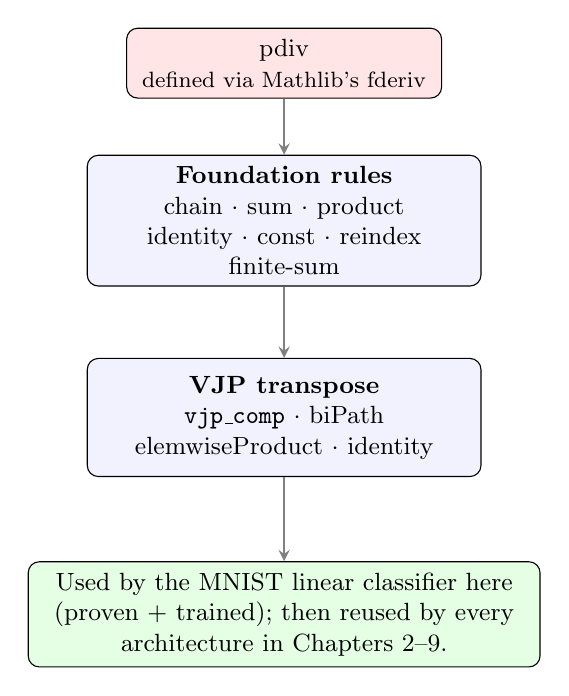
\begin{tikzpicture}[
  node distance=1.2cm,
  every node/.style={font=\small, align=center},
  group/.style={rectangle, draw, fill=blue!5, rounded corners,
                inner sep=4pt, minimum width=5cm, minimum height=1.5cm},
  root/.style={rectangle, draw, fill=red!10, rounded corners,
               inner sep=4pt, minimum width=4cm, minimum height=0.8cm},
  payoff/.style={rectangle, draw, fill=green!10, rounded corners,
                 inner sep=4pt, minimum width=6.5cm, minimum height=1cm},
  arrow/.style={->, >=stealth, thick, gray}
]
\node[root] (pdiv) at (0, 5) {\(\pdiv\) \\ \footnotesize defined via Mathlib's \(\fderiv\)};

\node[group] (foundation) at (0, 3) {\textbf{Foundation rules} \\ chain $\cdot$ sum $\cdot$ product \\ identity $\cdot$ const $\cdot$ reindex \\ finite-sum};

\node[group] (vjp) at (0, 0.5) {\textbf{VJP transpose} \\ \texttt{vjp\_comp} $\cdot$ biPath \\ elemwiseProduct $\cdot$ identity};

\node[payoff] (payoff) at (0, -2) {Used by the MNIST linear classifier here \\ (proven + trained); then reused by every \\ architecture in Chapters 2--9.};

\draw[arrow] (pdiv) -- (foundation);
\draw[arrow] (foundation) -- (vjp);
\draw[arrow] (vjp) -- (payoff);
\end{tikzpicture}
\end{center}

Read top-to-bottom, this is the order things get proved.
Read bottom-to-top, this is what every theorem in Chapters
3--9 unfolds to. (Ch~\ref{chap:attention} attention adds
matrix-level machinery on top. See \S\ref{sec:matrix_machinery}.) The full clickable dependency
graph is in the blueprint web view.

\paragraph{How the proofs are written.}
The proofs in this book follow Lamport's structured style
(\href{https://lamport.azurewebsites.net/pubs/proof.pdf}{\emph{How to
Write a 21\textsuperscript{st} Century Proof}}).
Hypotheses are named up front in an \Assume{}/\Prove{} header, with the
matching Lean hypothesis name in brackets. The proof is a numbered
sequence of steps. Each step carries its own \textsc{proof} naming
exactly the facts it follows from, and the final step is always \Qed{},
which explains why the steps prove the goal. In equational chains,
\(\prev\) stands for the expression established by the previous step.
Each step mirrors one tactic block of the corresponding Lean proof, so
the informal argument can be audited against the formal one step by
step. One-line lemmas (\texttt{pdiv\_id}, \texttt{pdiv\_const},
\texttt{pdiv\_reindex}, the identity VJP) stay unstructured:
structuring a one-\texttt{simp} proof would be ceremony.

\section{The theorems}

\begin{definition}[Partial derivative]
  \label{ax:pdiv}
  \lean{Proofs.pdiv}
  \leanok
  The partial derivative function. For \(f : \Vect{m} \to \Vect{n}\),
  \(\pdiv\, f\, x\, i\, j\) is the \((i, j)\)-entry of the Jacobian at \(x\),
  defined as \(\fderiv_{\R}\, f\, x\, (\basisVec_i)\, j\) — the
  \(j\)-th coordinate of Mathlib's Fréchet derivative applied to the
  \(i\)-th standard basis vector.
\end{definition}

\begin{theorem}[Chain rule]
  \label{ax:pdiv_comp}
  \lean{Proofs.pdiv_comp}
  \leanok
  \uses{ax:pdiv}
  \Assume{}
  \begin{enumerate}
    \item \(f : \Vect{m} \to \Vect{n}\) is differentiable at \(x\)
          \hfill[\texttt{hf}]
    \item \(g : \Vect{n} \to \Vect{p}\) is differentiable at \(f(x)\)
          \hfill[\texttt{hg}]
  \end{enumerate}
  \Prove{} for all \(i, k\):
  \[
    \pdiv(g \circ f)\, x\, i\, k
      = \sum_j \pdiv f\, x\, i\, j \cdot \pdiv g\, (f\, x)\, j\, k.
  \]
\end{theorem}

\begin{proof}
\leanok
\emph{Sketch: reduce to Mathlib's chain rule for \(\fderiv\), then
decompose over the standard basis to turn a composite of linear maps
into the sum over the middle index.}
\begin{enumerate}
  \item \(\pdiv(g \circ f)\, x\, i\, k
          = \fderiv_{\R}\,(g \circ f)\, x\, (\basisVec_i)\, k\).
    \pf{Definition~\ref{ax:pdiv}.}
  \item \(\fderiv_{\R}\,(g \circ f)\, x
          = \fderiv_{\R}\, g\, (f\,x) \circ \fderiv_{\R}\, f\, x\).
    \pf{Mathlib's \texttt{fderiv\_comp}, applicable by assumptions 1
    and 2.}
  \item Let \(v := \fderiv_{\R}\, f\, x\, (\basisVec_i) \in \Vect{n}\).
    Then \(v = \sum_j v_j \cdot \basisVec_j\).
    \pf{Pointwise: at coordinate \(j'\) the sum collapses to
    \(v_{j'}\), because \((\basisVec_j)_{j'}\) is the Kronecker
    delta.}
  \item \(\fderiv_{\R}\, g\, (f\,x)\, v\, k
          = \sum_j v_j \cdot \fderiv_{\R}\, g\, (f\,x)\, (\basisVec_j)\, k\).
    \pf{By 3 and linearity of \(\fderiv_{\R}\, g\, (f\,x)\)
    (\texttt{map\_sum}, \texttt{map\_smul}).}
  \item \Qed{}
    \pf{By Definition~\ref{ax:pdiv}, \(v_j = \pdiv f\, x\, i\, j\) and
    \(\fderiv_{\R}\, g\, (f\,x)\, (\basisVec_j)\, k
      = \pdiv g\, (f\,x)\, j\, k\); chaining 1, 2, and 4 gives the
    goal.}
\end{enumerate}
\end{proof}

\begin{theorem}[Sum rule]
  \label{ax:pdiv_add}
  \lean{Proofs.pdiv_add}
  \leanok
  \uses{ax:pdiv}
  \Assume{}
  \begin{enumerate}
    \item \(f, g : \Vect{m} \to \Vect{n}\) are both differentiable at
          \(x\) \hfill[\texttt{hf}, \texttt{hg}]
  \end{enumerate}
  \Prove{} for all \(i, j\):
  \[
    \pdiv(f + g)\, x\, i\, j = \pdiv f\, x\, i\, j + \pdiv g\, x\, i\, j.
  \]
\end{theorem}

\begin{proof}
\leanok
\begin{enumerate}
  \item \(\pdiv(f + g)\, x\, i\, j
          = \fderiv_{\R}\,(f + g)\, x\, (\basisVec_i)\, j\).
    \pf{Definition~\ref{ax:pdiv}; the pointwise sum
    \(\lambda y\, k.\; f\,y\,k + g\,y\,k\) is definitionally the
    function \(f + g\).}
  \item \(\fderiv_{\R}\,(f + g)\, x
          = \fderiv_{\R}\, f\, x + \fderiv_{\R}\, g\, x\).
    \pf{Mathlib's \texttt{fderiv\_add}, applicable by the assumption.}
  \item \Qed{}
    \pf{Evaluate 2 at \((\basisVec_i, j)\); by
    Definition~\ref{ax:pdiv} the two terms are
    \(\pdiv f\, x\, i\, j\) and \(\pdiv g\, x\, i\, j\).}
\end{enumerate}
\end{proof}

\begin{theorem}[Product rule]
  \label{ax:pdiv_mul}
  \lean{Proofs.pdiv_mul}
  \leanok
  \uses{ax:pdiv}
  \Assume{}
  \begin{enumerate}
    \item \(f, g : \Vect{m} \to \Vect{n}\) are both differentiable at
          \(x\) \hfill[\texttt{hf}, \texttt{hg}]
  \end{enumerate}
  \Prove{} for all \(i, j\):
  \[
    \pdiv(f \odot g)\, x\, i\, j
      = \pdiv f\, x\, i\, j \cdot g\, x\, j
      + f\, x\, j \cdot \pdiv g\, x\, i\, j,
  \]
  where \((f \odot g)\, y\, k = f\,y\,k \cdot g\,y\,k\) is the
  elementwise product.
\end{theorem}

\begin{proof}
\leanok
\begin{enumerate}
  \item \(\pdiv(f \odot g)\, x\, i\, j
          = \fderiv_{\R}\,(f \cdot g)\, x\, (\basisVec_i)\, j\).
    \pf{Definition~\ref{ax:pdiv}; the elementwise product is
    definitionally the algebra product \(f \cdot g\) in \(\Vect{n}\)
    (\texttt{Pi.normedAlgebra}), so Mathlib's calculus of
    algebra-valued maps applies.}
  \item \(\fderiv_{\R}\,(f \cdot g)\, x
          = f\,x \cdot \fderiv_{\R}\, g\, x
          + g\,x \cdot \fderiv_{\R}\, f\, x\)
    (scalar action taken pointwise).
    \pf{Mathlib's \texttt{fderiv\_mul}, applicable by the assumption.}
  \item \Qed{}
    \pf{Evaluate 2 at \((\basisVec_i, j)\): the pointwise scalar
    action gives
    \(f\,x\,j \cdot \pdiv g\, x\, i\, j + g\,x\,j \cdot \pdiv f\, x\, i\, j\)
    by Definition~\ref{ax:pdiv}; commute the second summand
    (\texttt{ring}) to match the goal.}
\end{enumerate}
\end{proof}

\begin{theorem}[Identity Jacobian]
  \label{ax:pdiv_id}
  \lean{Proofs.pdiv_id}
  \leanok
  \uses{ax:pdiv}
  \(\pdiv(\mathrm{id})\, x\, i\, j = \delta_{ij}\).
\end{theorem}

\begin{proof}
\leanok
Mechanical; see \leandocref{Proofs.pdiv\_id}.
\end{proof}

\begin{theorem}[Constant has zero Jacobian]
  \label{ax:pdiv_const}
  \lean{Proofs.pdiv_const}
  \leanok
  \uses{ax:pdiv}
\end{theorem}

\begin{proof}
\leanok
Mechanical; see \leandocref{Proofs.pdiv\_const}.
\end{proof}

\begin{theorem}[Gather / reindex Jacobian]
  \label{ax:pdiv_reindex}
  \lean{Proofs.pdiv_reindex}
  \leanok
  \uses{ax:pdiv}
  Covers permutations, reshapes, slicing. Generalizes \texttt{pdiv\_id}.
\end{theorem}

\begin{proof}
\leanok
Mechanical; see \leandocref{Proofs.pdiv\_reindex}.
\end{proof}

\begin{theorem}[Finite-sum rule]
  \label{thm:pdiv_finset_sum}
  \lean{Proofs.pdiv_finset_sum}
  \leanok
  \uses{ax:pdiv, ax:pdiv_add, ax:pdiv_const}
  \Assume{}
  \begin{enumerate}
    \item \(S\) is a finite index set with a function
          \(f_s : \Vect{m} \to \Vect{n}\) for each \(s \in S\)
    \item every \(f_s\) is differentiable at \(x\)
          \hfill[\texttt{hdiff}]
  \end{enumerate}
  \Prove{} for all \(i, j\):
  \[
    \pdiv\Bigl(\sum_{s \in S} f_s\Bigr)\, x\, i\, j
      = \sum_{s \in S} \pdiv f_s\, x\, i\, j.
  \]
\end{theorem}

\begin{proof}
\leanok
\emph{Sketch: induction on \(S\); the two-summand sum rule does each
inductive step.}
\begin{enumerate}
  \item \Case{} \(S = \emptyset\): both sides are \(0\).
    \pf{The empty sum is the constant zero function, whose Jacobian
    vanishes by Theorem~\ref{ax:pdiv_const}; the right side is an
    empty sum.}
  \item \Case{} \(S = \{a\} \cup T\) with \(a \notin T\), assuming the
    claim holds for \(T\) (induction hypothesis):
    \(\pdiv\bigl(\sum_{s \in S} f_s\bigr)\, x\, i\, j
      = \pdiv f_a\, x\, i\, j + \sum_{s \in T} \pdiv f_s\, x\, i\, j\).
    \pf{Split the sum as \(f_a + \sum_{s \in T} f_s\)
    (\texttt{Finset.sum\_insert}, using \(a \notin T\)). The tail
    \(\sum_{s \in T} f_s\) is differentiable at \(x\) as a finite sum
    of functions differentiable by assumption 2
    (\texttt{DifferentiableAt.fun\_sum}), so the sum rule
    (Theorem~\ref{ax:pdiv_add}) splits the Jacobian; the induction
    hypothesis rewrites the tail.}
  \item \Qed{}
    \pf{By induction on the finite set \(S\)
    (\texttt{Finset.induction\_on}): 1 is the base case, and
    re-merging the sum in 2 gives the inductive step.}
\end{enumerate}
\end{proof}

\begin{definition}[VJP record]
  \label{def:hasvjp}
  \lean{Proofs.HasVJP}
  \leanok
  \uses{ax:pdiv}
  For \(f : \Vect{m} \to \Vect{n}\), \(\HasVJP\, f\) bundles a backward
  function \(B : \Vect{m} \to \Vect{n} \to \Vect{m}\) with its
  correctness claim: for all \(x\), \(dy\), \(i\),
  \[
    B(x, dy)_i = \sum_j \pdiv f\, x\, i\, j \cdot dy_j.
  \]
  Exhibiting a \(\HasVJP\, f\) is exactly the statement ``this backward
  function computes the vector--Jacobian product of \(f\).''
\end{definition}

\begin{theorem}[VJP chain rule]
  \label{thm:vjp_comp}
  \lean{Proofs.vjp_comp}
  \leanok
  \uses{ax:pdiv, ax:pdiv_comp, def:hasvjp}
  \Assume{}
  \begin{enumerate}
    \item \(B_f\) is a correct backward function for \(f\)
          (\(\HasVJP\, f\)) \hfill[\texttt{hf}]
    \item \(B_g\) is a correct backward function for \(g\)
          (\(\HasVJP\, g\)) \hfill[\texttt{hg}]
    \item \(f\) is differentiable everywhere \hfill[\texttt{hf\_diff}]
    \item \(g\) is differentiable everywhere \hfill[\texttt{hg\_diff}]
  \end{enumerate}
  \Prove{} \(\HasVJP\, (g \circ f)\).
\end{theorem}

\begin{proof}
\leanok
\emph{Sketch: the composite backward is ``run \(B_g\), feed the result
to \(B_f\)''; correctness is the two \texttt{correct} fields glued by
the chain rule for \(\pdiv\).}
\begin{enumerate}
  \item Define \(B(x, dy) := B_f\bigl(x,\; B_g(f\,x,\; dy)\bigr)\).
  \item \Suffices{} for all \(x\), \(dy\), \(i\):
    \(B(x, dy)_i = \sum_k \pdiv(g \circ f)\, x\, i\, k \cdot dy_k\).
    \pf{Definition~\ref{def:hasvjp}, with \(B\) as the candidate
    backward function.}
  \item \(B(x, dy)_i
          = \sum_j \pdiv f\, x\, i\, j \cdot B_g(f\,x, dy)_j\).
    \pf{Correctness of \(B_f\) (assumption 1).}
  \item \(\prev = \sum_j \pdiv f\, x\, i\, j
          \sum_k \pdiv g\, (f\,x)\, j\, k \cdot dy_k\).
    \pf{Correctness of \(B_g\) (assumption 2).}
  \item \(\prev = \sum_k \Bigl(\sum_j \pdiv f\, x\, i\, j
          \cdot \pdiv g\, (f\,x)\, j\, k\Bigr)\, dy_k\).
    \pf{Distribute and swap the two sums (\texttt{Finset.mul\_sum},
    \texttt{Finset.sum\_comm}); both are finite, so no convergence
    question arises.}
  \item \Qed{}
    \pf{By the chain rule (Theorem~\ref{ax:pdiv_comp}), applicable at
    every \(x\) by assumptions 3 and 4, the inner sum in 5 is
    \(\pdiv(g \circ f)\, x\, i\, k\); with 2 this is the goal.}
\end{enumerate}
\end{proof}

\begin{theorem}[Additive fan-in VJP]
  \label{thm:biPath_has_vjp}
  \lean{Proofs.biPath_has_vjp}
  \leanok
  \uses{ax:pdiv, ax:pdiv_add, def:hasvjp}
  Used for residual connections.
  \Assume{}
  \begin{enumerate}
    \item \(B_f\) is a correct backward function for \(f\)
          (\(\HasVJP\, f\)) \hfill[\texttt{hf}]
    \item \(B_g\) is a correct backward function for \(g\)
          (\(\HasVJP\, g\)) \hfill[\texttt{hg}]
    \item \(f\) is differentiable everywhere \hfill[\texttt{hf\_diff}]
    \item \(g\) is differentiable everywhere \hfill[\texttt{hg\_diff}]
  \end{enumerate}
  \Prove{} \(\HasVJP\, (f + g)\).
\end{theorem}

\begin{proof}
\leanok
\begin{enumerate}
  \item Define \(B(x, dy)_i := B_f(x, dy)_i + B_g(x, dy)_i\).
  \item \Suffices{} for all \(x\), \(dy\), \(i\):
    \(B(x, dy)_i = \sum_j \pdiv(f + g)\, x\, i\, j \cdot dy_j\).
    \pf{Definition~\ref{def:hasvjp}, with \(B\) as the candidate
    backward function.}
  \item \(B(x, dy)_i = \sum_j \bigl(\pdiv f\, x\, i\, j
          + \pdiv g\, x\, i\, j\bigr) \cdot dy_j\).
    \pf{Correctness of \(B_f\) and \(B_g\) (assumptions 1, 2); merge
    the two finite sums (\texttt{Finset.sum\_add\_distrib}) and factor
    out \(dy_j\) (\texttt{ring}).}
  \item \Qed{}
    \pf{The sum rule (Theorem~\ref{ax:pdiv_add}), applicable at every
    \(x\) by assumptions 3 and 4, rewrites the bracket in 3 to
    \(\pdiv(f + g)\, x\, i\, j\); with 2 this is the goal.}
\end{enumerate}
\end{proof}

\begin{theorem}[Multiplicative fan-in VJP]
  \label{thm:elemwiseProduct_has_vjp}
  \lean{Proofs.elemwiseProduct_has_vjp}
  \leanok
  \uses{ax:pdiv, ax:pdiv_mul, def:hasvjp}
  Used for Squeeze-and-Excitation.
  \Assume{}
  \begin{enumerate}
    \item \(B_f\) is a correct backward function for \(f\)
          (\(\HasVJP\, f\)) \hfill[\texttt{hf}]
    \item \(B_g\) is a correct backward function for \(g\)
          (\(\HasVJP\, g\)) \hfill[\texttt{hg}]
    \item \(f\) is differentiable everywhere \hfill[\texttt{hf\_diff}]
    \item \(g\) is differentiable everywhere \hfill[\texttt{hg\_diff}]
  \end{enumerate}
  \Prove{} \(\HasVJP\, (f \odot g)\), where
  \((f \odot g)\, x\, i = f\,x\,i \cdot g\,x\,i\).
\end{theorem}

\begin{proof}
\leanok
\begin{enumerate}
  \item Define \(B(x, dy)_i
          := B_f\bigl(x,\; g(x) \odot dy\bigr)_i
          + B_g\bigl(x,\; f(x) \odot dy\bigr)_i\),
    where \(\bigl(g(x) \odot dy\bigr)_j = g\,x\,j \cdot dy_j\).
  \item \Suffices{} for all \(x\), \(dy\), \(i\):
    \(B(x, dy)_i = \sum_j \pdiv(f \odot g)\, x\, i\, j \cdot dy_j\).
    \pf{Definition~\ref{def:hasvjp}, with \(B\) as the candidate
    backward function.}
  \item \(B(x, dy)_i = \sum_j \bigl(\pdiv f\, x\, i\, j \cdot g\,x\,j
          + f\,x\,j \cdot \pdiv g\, x\, i\, j\bigr) \cdot dy_j\).
    \pf{Correctness of \(B_f\) at upstream gradient \(g(x) \odot dy\)
    and of \(B_g\) at \(f(x) \odot dy\) (assumptions 1, 2); merge the
    two finite sums and factor out \(dy_j\)
    (\texttt{Finset.sum\_add\_distrib}, \texttt{ring}).}
  \item \Qed{}
    \pf{The product rule (Theorem~\ref{ax:pdiv_mul}), applicable at
    every \(x\) by assumptions 3 and 4, identifies the bracket in 3
    with \(\pdiv(f \odot g)\, x\, i\, j\); with 2 this is the goal.}
\end{enumerate}
\end{proof}

\begin{theorem}[Identity VJP]
  \label{thm:identity_has_vjp}
  \lean{Proofs.identity_has_vjp}
  \leanok
  \uses{ax:pdiv, ax:pdiv_id, def:hasvjp}
\end{theorem}

\begin{proof}
\leanok
Mechanical; see \leandocref{Proofs.identity\_has\_vjp}.
\end{proof}

\section{Example: MNIST linear classifier}

The smallest network that learns: a single dense layer mapping
784-dim images to 10-dim logits, trained with softmax cross-entropy
and plain SGD. About 7,850 parameters. \(\sim\)92\% test accuracy
in seconds.

\begin{center}
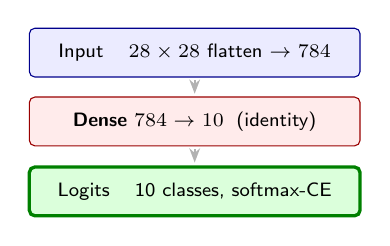
\begin{tikzpicture}[
  >={Stealth[length=1.8mm]},
  every node/.style={font=\sffamily\scriptsize},
  col/.style    = {align=center, rounded corners=2pt, inner sep=2pt, minimum height=0.62cm, minimum width=4.2cm},
  io/.style     = {col, draw=blue!55!black,   fill=blue!8},
  head/.style   = {col, draw=red!60!black,    fill=red!8},
  logits/.style = {col, draw=green!50!black,  fill=green!14, very thick},
  arr/.style    = {->, thick, gray!60, shorten >=1pt, shorten <=1pt},
]
  % Vertical layer column: the whole "network" is one dense layer.
  \node[io]                           (input) {Input \;\; $28\times28$ flatten $\to 784$};
  \node[head, below=0.24cm of input]  (d1)    {\textbf{Dense} $784\to10$ \;(identity)};
  \node[logits, below=0.24cm of d1]   (out)   {Logits \;\; 10 classes, softmax-CE};
  \foreach \a/\b in {input/d1, d1/out}
     \draw[arr] (\a) -- (\b);
\end{tikzpicture}
\end{center}

\paragraph{The forward pass and loss, in math.}
For an input image \(x \in \R^{784}\) and true class index
\(t \in \{0, \dots, 9\}\):
\begin{align*}
  z &= W x + b
    &&\text{(dense layer; \(W \in \R^{10 \times 784}\), \(b \in \R^{10}\))} \\
  \hat{y}_i &= \mathrm{softmax}(z)_i = \frac{e^{z_i}}{\sum_j e^{z_j}}
    &&\text{(class probabilities)} \\
  \ell(W, b;\, x, t) &= -\log \hat{y}_t
    &&\text{(cross-entropy on the true class)}
\end{align*}
The trainable parameters are \(W\) and \(b\), which is 7,850 floats
in total.

\paragraph{The same thing, as a \texttt{VerifiedNetSpec}.}
\begin{verbatim}
def linearVerified : VerifiedNetSpec where
  name     := "MNIST-Linear"
  slug     := "linear"
  inC      := 1
  imageH   := 28
  imageW   := 28
  nClasses := 10
  data     := .mnist
  layers   := [.dense 784 10]
\end{verbatim}

The layer emits raw logits \(z = W x + b\). Softmax and cross-entropy
are added by the training driver, because this is a classification
task. The \texttt{slug} names the committed render, so this spec is
bound to \texttt{verified\_mlir/linear\_train\_step.mlir} and
\texttt{linear\_fwd.mlir}, which are the two files the run at the top of
the chapter compiled.

\paragraph{What \texttt{.dense 784 10} contributes.} Layers are
constructors of a \texttt{VLayer} inductive, and one function,
\texttt{toSpecs}, says what each contributes to the parameter list as
\texttt{(dims, initKind)} pairs --- \texttt{0} is He(fan-in), \texttt{1}
is ones, \texttt{2} is zeros:

\begin{verbatim}
def toSpecs : VLayer -> Array (Array Nat × Nat)
  | dense ic oc => #[(#[ic,oc],0),(#[oc],2)]
  | ...
\end{verbatim}

\noindent Two tensors: a $784 \times 10$ weight matrix initialised
He(fan-in), and a length-10 bias initialised to zero. That is this
network's entire parameter list, and \texttt{d0}, the input width the
render needs, is derived from the same list rather than declared
separately. Every chapter after this one adds an arm to that match.
None of them changes this one, so this is the last time you will see it.

That binding is why the type exists. The spec lives in
\texttt{LeanMlir/VerifiedNets.lean} rather than beside the trainer,
because the theorem and the program have to name the same object. In
\texttt{LeanMlir/Proofs/Foundation/SpecVJP.lean}:

\begin{verbatim}
noncomputable def linearVerified_has_vjp (W : Mat 784 10) (b : Vec 10) :
    HasVJP (denoteLinear linearVerified.layers W b) :=
  dense_has_vjp W b
\end{verbatim}

Read the type. The VJP is proved for the denotation of
\texttt{linearVerified.layers}, and that is the same field the trainer
reads to build its graph. Copy the layer list into a second definition
and the proof would be about a different network than the one that runs.

\paragraph{The whole program.}
The trainer is 53 lines including its docstring, so here it is entire,
with the comments stripped:

\begin{verbatim}
import LeanMlir.VerifiedNets

def linearConfig : VerifiedConfig where
  epochs    := 12
  batchSize := 128

def main (argv : List String) : IO Unit :=
  linearVerified.trainLinear linearConfig (argv.head?.getD "data")
\end{verbatim}

That is \texttt{apps/mnist/MainMnistLinearVerified.lean}, all of it. One
spec, one config, one call. The GPU backend does not appear in it at all,
because the shim is opened with \texttt{dlopen} at run time.

Notice also what \texttt{linearConfig} does not carry: a learning rate.
The real rate is baked into
\texttt{verified\_mlir/linear\_train\_step.mlir} at render time, so the
recipe that trains is the recipe the proofs describe, and the two cannot
drift apart.

\paragraph{The gradient, in math.}
Backpropagation through this network produces a single outer
product:
\[
  \nabla_W \ell = (\hat{y} - e_t) \otimes x, \qquad
  \nabla_b \ell = \hat{y} - e_t
\]
where \(e_t \in \R^{10}\) is the one-hot vector for the true
class. Ch~1's theorems (chain rule + identity Jacobian/VJP) plus
the Dense Jacobian and softmax-CE gradient (formalized in
Ch~\ref{chap:mlp}, both themselves proved from this chapter's
foundation rules) are what guarantee these formulas are correct. The
verified renderer emits exactly these as fused StableHLO, and that
rendering is \texttt{verified\_mlir/linear\_train\_step.mlir}, the file
the run at the top of the chapter compiled.

\paragraph{Results.}
The run at the top of this chapter is this network. Accuracy climbs from
89.77\% after one epoch to 92.10\% after twelve, and the curve is
essentially flat from epoch~9 on, which is what a model with no hidden
layer looks like once it has learned everything it can. Adding hidden
layers and ReLU in Chapter~\ref{chap:mlp} takes the same dataset and the
same recipe to 97.83\%. That gap of about 5.7 points is the value of
non-linearity on this task.

\paragraph{Where this goes.}
Every architecture in Part~2 extends this template the same way, one
new primitive at a time:

\begin{itemize}
  \item Ch~\ref{chap:mlp} stacks dense layers and inserts ReLU between
    them. One new operator VJP.
  \item Ch~\ref{chap:cnn} swaps the dense forward for conv2d. One new
    operator VJP.
  \item Ch~\ref{chap:bn} adds BatchNorm. One new operator VJP.
  \item Ch~\ref{chap:residual} adds the residual skip. Additive fan-in,
    Theorem~\ref{thm:biPath_has_vjp}, and no new operator at all.
  \item Ch~\ref{chap:depthwise} factors standard conv into depthwise
    plus pointwise. One new operator VJP, recombined through the chain
    rule.
  \item Ch~\ref{chap:se} adds the SE channel-attention block, which is
    an elementwise product over global pooling and dense layers. One new
    VJP composed from pieces we already have.
  \item Ch~\ref{chap:layernorm} replaces ReLU with GELU. One new
    operator.
  \item Ch~\ref{chap:attention} adds attention, which needs new
    matrix-level machinery and softmax-VJP chains.
\end{itemize}
 The structural
rules from this chapter never change. Later chapters add
operator-specific theorems and compose them through the chain rule we
just proved. The driver that runs all of them is the same Lean either
way, and it is shorter than you would expect, which is the subject of
\S\ref{sec:mlp_inside_train}.

\section{MLIR: Linear}

The StableHLO in this section is the artifact the proofs are about, and
it is what XLA compiles and runs. Nothing between the theorem and the GPU
rewrites it.

The forward half is short enough to print whole. This is
\texttt{verified\_mlir/linear\_fwd.mlir} exactly as committed, and it is
one of the two files the run at the top of the chapter compiled:

\begin{verbatim}
module @m {
  func.func @linear_fwd(%x: tensor<128x784xf32>,
                        %W0: tensor<784x10xf32>,
                        %b0: tensor<10xf32>) -> tensor<128x10xf32> {
    %v0 = stablehlo.dot_general %x, %W0,
            contracting_dims = [1] x [0],
            precision = [DEFAULT, DEFAULT]
            : (tensor<128x784xf32>, tensor<784x10xf32>)
              -> tensor<128x10xf32>
    %v1 = stablehlo.broadcast_in_dim %b0, dims = [1]
            : (tensor<10xf32>) -> tensor<128x10xf32>
    %v2 = stablehlo.add %v0, %v1 : tensor<128x10xf32>
    return %v2 : tensor<128x10xf32>
  }
}
\end{verbatim}

Three operations for \(z = Wx + b\): a contraction, a broadcast of the
bias across the batch, and an add. The shapes are the real ones, batch
128 against 784 inputs and 10 classes, because this file is the render
that trains and not an illustration of one.

The backward pass is one operation. With the loss cotangent
$dy = \mathrm{softmax}(\mathrm{logits}) - \text{onehot}$, the input
gradient is $dx = dy\,W^{\!\top}$, a single matrix multiply. Here is
what the code generator emits for it, shown at a small representative
size so the shapes stay readable:

\begin{verbatim}
func.func @linear_back(%dy: tensor<2x3xf32>, %W0: tensor<4x3xf32>)
    -> tensor<2x4xf32> {
  %bk0 = stablehlo.dot_general %dy, %W0, contracting_dims = [1] x [1]
           : (tensor<2x3xf32>, tensor<4x3xf32>) -> tensor<2x4xf32>
  return %bk0 : tensor<2x4xf32>
}
\end{verbatim}

\noindent That \texttt{dot\_general} contracts the output axis of $dy$ against the
output axis of $W$, which is multiplication by $W^{\!\top}$, and by a
machine-checked theorem that is the linear layer's exact reverse-mode
derivative. Everything else in this book scales that one move up. Each
architecture chapter closes with an ``MLIR: operator'' section that takes
the chapter's new operator and shows that its emitted backward is
likewise the rendering of a proven derivative. Those operators are
convolution, BatchNorm, the residual fan-in, depthwise convolution,
squeeze-excitation, layer scale, and attention.

Each of those listings is shown at a small representative size, meaning a
few channels, tokens, or units of width. The per-operator proof beneath
is dimension-parameterized and the printer emits the identical graph at
production scale, so each section states its toy shape and moves on.
Appendix~\ref{app:verification} covers the shared machinery underneath
them: the denoted intermediate representation, the bridge theorems that
tie it to the proofs, the printer that turns it into the text above, and
the execution oracle that checks the result on the GPU.

\section{What's inside \texttt{.train}?}
\label{sec:mlp_inside_train}

The section above treated \texttt{linearVerified.trainLinear} as a black
box. You named the network, you named the epochs and the batch size, and
training happened. That is deliberately the user-facing interface, but
there is no magic underneath it. The driver is ordinary Lean in
\texttt{LeanMlir/VerifiedTrain.lean}, and the interesting thing about it
is how little it does.

\paragraph{The training loop, the way a math book would write it.}
\begin{verbatim}
Algorithm: Mini-batch SGD, with the step compiled into the graph
Input:  net (a VerifiedNetSpec), cfg (epochs, batch size),
        dataset D = (X_train, y_train, X_test, y_test)
Output: trained parameters (W, b)

// 1. Open sessions over the two committed renders
ts  <- session(verified_mlir/<slug>_train_step.mlir)
fwd <- session(verified_mlir/<slug>_fwd.mlir)

// 2. Load data; zero-initialise the parameters
(X, y), (Xt, yt) <- load(D)
(W, b) <- 0

// 3. Epoch loop
for epoch = 1 to cfg.epochs:

    // 4. Batch loop: ONE call per batch
    for each mini-batch (x, t) of size B:
        (W, b) <- ts(x, W, b, onehot(t))

    // 5. Evaluate on the whole test set
    eval(fwd, W, b, Xt, yt)
\end{verbatim}

\paragraph{What is missing from that loop, and where it went.}
Compare it to the loop any framework tutorial shows you. There is no
gradient variable. There is no optimizer call. There is no
learning-rate schedule. Those three lines were not dropped, they moved
into \texttt{verified\_mlir/linear\_train\_step.mlir}, which is where
they can be proved. The loop above cannot get the update rule wrong,
because it does not implement the update rule.

That is the difference between this driver and a conventional one, and
it is worth being precise about what it buys. A bug in a hand-written
optimizer is a bug you find by watching the loss curve look strange. A
bug in the rendered optimizer is a bug that fails a theorem at build
time. Moving the arithmetic into the graph moves it inside the reach of
the proofs.

\paragraph{The same loop, in Lean.}
Here is the real thing, \texttt{VerifiedNet.trainLinear}, in full. Only
the per-epoch timing and two environment-variable overrides are dropped;
every line that computes the answer is here:

\begin{verbatim}
def VerifiedNet.trainLinear (net : VerifiedNet) (cfg : VerifiedConfig)
    (dataDir : String) : IO Unit := do
  let bs := cfg.batchSize
  let d0 := net.d0
  let d1 := net.nClasses

  -- 1. One session per committed render
  let tsSess  <- mkSession s!"{net.mlirDir}/{net.slug}_train_step.mlir"
  let fwdSess <- mkSession s!"{net.mlirDir}/{net.slug}_fwd.mlir"

  -- 2. Data, then zero-initialised parameters
  let (trainImg, trainLbl, nTrain, evalImg, evalLbl, nEval, _, _) <-
    loadData net dataDir
  let mut W0 <- F32.const (d0 * d1).toUSize 0.0
  let mut b0 <- F32.const d1.toUSize 0.0
  let nb     := nTrain / bs
  let nbt    := (nEval + bs - 1) / bs   -- ceil: last eval batch is zero-padded
  let pBytes := (d0 * d1 + d1) * 4
  let shapes := net.shapesBA            -- packed [W0|b0] layout for the forward
  let xShape := net.xShape bs
  let mut packed := W0 ++ b0

  -- 3. Epoch loop
  for ep in [0:cfg.epochs] do

    -- 4. Batch loop: forward, loss, backward, SGD -- one call
    for bi in [0:nb] do
      let xb := F32.sliceImages trainImg (bi * bs) bs d0
      let yb := F32.sliceLabels trainLbl (bi * bs) bs
      let out <- LowererSession.linearTrainStepV tsSess tsFn
                   xb W0 b0 yb bs.toUSize d0.toUSize d1.toUSize nResident
      packed := out
      W0 := out.extract 0 (d0 * d1 * 4)
      b0 := out.extract (d0 * d1 * 4) pBytes

    -- 5. Evaluate on the full test set, every epoch
    let params <- LowererSession.readParams tsSess packed pBytes.toUSize
    let mut correct := 0
    for bi in [0:nbt] do
      let xb := F32.sliceImagesPad evalImg (bi * bs) bs d0 nEval
      let logits <- LowererSession.forwardF32 fwdSess fwdFn params shapes
                      xb xShape bs.toUSize d1.toUSize nResident (ep+1).toUSize
      for j in [0:min bs (nEval - bi * bs)] do  -- real rows only, not the pad
        let pred := (F32.argmaxN logits (j * d1).toUSize d1.toUSize).toNat
        if pred == F32.readLabel evalLbl (bi * bs + j) then
          correct := correct + 1
    let acc := correct.toFloat / nEval.toFloat * 100.0
    IO.println s!"  epoch {ep+1}: test_acc = {correct}/{nEval} = {acc}%"
\end{verbatim}

Walking through the numbered sections:

\textbf{1. Sessions.} \texttt{mkSession} takes the path to a committed
\texttt{.mlir}, hands it to the shim, and gets back something callable.
XLA compiles the StableHLO in process, which is the 714\,ms the run
reported.

\textbf{2. Data and initialisation.} \texttt{loadData} mmaps the on-disk
binaries into \texttt{F32Array} buffers. \texttt{trainImg} holds
flattened pixels and \texttt{trainLbl} holds integer class labels.
Weights start at zero rather than He-initialised, which is fine for a
model with no hidden layer and no symmetry to break.

\textbf{3. Epoch loop.} Twelve passes over the training set. Notice what
is not here: no learning-rate computation, because the rate is baked
into the render.

\textbf{4. Batch loop, the core of training.} Slice a batch of images
and labels, then call \texttt{linearTrainStepV}. That one call does
everything: the forward pass, the cross-entropy loss, the backward pass
built from the VJPs proved earlier in this chapter, and the SGD update.
It returns the new parameters packed as \texttt{[W0|b0]}.

This one line is where the whole pipeline pays off. There is no Python.
There is no per-step graph construction. There is no autograd
interpreter walking a tape. The training step was compiled once at
startup, in 714\,ms, and every batch after that is a single dispatched
call. Chapter~1's run does 468 of those per epoch and finishes an epoch
in about 235\,ms including a full pass over the 10,000 test images.

\textbf{5. Validation.} Every epoch, not every tenth, because a forward
pass over the test set is cheap next to the training epoch. Two details
are worth naming now because every later chapter inherits them. The
eval loop reads the parameters back with \texttt{readParams} rather than
using the \texttt{W0}/\texttt{b0} it already has, because under device
residency those two are stale by design and \texttt{packed} is the
authoritative copy. And \texttt{nbt} rounds \emph{up}: the last eval
batch is zero-padded to \texttt{bs} and the inner loop scores only the
real rows, so a test set whose size is not a multiple of the batch size
is fully scored rather than silently truncated. Ten thousand images and
a batch of 128 would otherwise drop the last 16. The
forward-only render is a separate artifact rather than a branch inside
the training graph, which matters more in Chapter~\ref{chap:bn} where
BatchNorm has to use running statistics at inference and per-batch
estimates during training.

That is the whole function. The reason it is short is that everything
heavyweight lives in one compiled graph on the GPU. Lean's job here is
not to compute gradients. It is to specify what the training step is,
prove that specification correct, and invoke it. Three concerns, cleanly
separated, and only the middle one is unusual.

Every chapter after this one hands a different \texttt{VerifiedNetSpec}
to the same driver. Only the spec changes. That is the framework pitch
in concrete form: once the driver is written and the layers are proved
one at a time, every architecture in the book runs through it with no
further infrastructure code. It all runs on your hardware, and
Appendix~\ref{app:getting_started} walks you through the toolchain
setup.
\section{MLIR: Training Step}
\label{sec:mlir_training_step}

Section~\ref{sec:mlp_inside_train} made a claim about the inner call. One
dispatched StableHLO graph does the forward pass, the loss, the backward
pass, and the optimizer update, with no tape and no per-step graph
construction. The ``MLIR: Linear'' section
above rendered a single operator's backward in isolation. Here is the
whole thing the linear classifier compiles to. It is short enough to show
essentially in full, with only the default \texttt{precision} attributes
dropped and the long type signatures wrapped for the page:

\begin{verbatim}
func.func @linear_train_step(
    %x: tensor<128x784xf32>,  %W0: tensor<784x10xf32>,
    %b0: tensor<10xf32>,      %onehot: tensor<128x10xf32>)
    -> (tensor<784x10xf32>, tensor<10xf32>) {
  // -- forward + softmax-CE cotangent (rendered from lossCotGraph) --
  %v0 = stablehlo.dot_general %x, %W0, contracting_dims = [1] x [0]
          : (tensor<128x784xf32>, tensor<784x10xf32>) -> tensor<128x10xf32>
  %v1 = stablehlo.broadcast_in_dim %b0, dims = [1]
          : (tensor<10xf32>) -> tensor<128x10xf32>
  %v2 = stablehlo.add %v0, %v1 : tensor<128x10xf32>          // logits
  %v3 = stablehlo.exponential %v2 : tensor<128x10xf32>
  %v4 = stablehlo.constant dense<0.0> : tensor<f32>
  %v5 = stablehlo.reduce(%v3 init: %v4)
          applies stablehlo.add across dimensions = [1]
          : (tensor<128x10xf32>, tensor<f32>) -> tensor<128xf32>
  %v6 = stablehlo.broadcast_in_dim %v5, dims = [0]
          : (tensor<128xf32>) -> tensor<128x10xf32>
  %v7 = stablehlo.divide %v3, %v6 : tensor<128x10xf32>       // softmax
  %v8 = stablehlo.subtract %v7, %onehot : tensor<128x10xf32> // dy
  // -- param grads:  dW0 = x^T . dy,  db0 = sum_batch dy --
  %sc  = stablehlo.constant dense<0.0> : tensor<f32>
  %dW0 = stablehlo.dot_general %x, %v8, contracting_dims = [0] x [0]
           : (tensor<128x784xf32>, tensor<128x10xf32>) -> tensor<784x10xf32>
  %db0 = stablehlo.reduce(%v8 init: %sc)
           applies stablehlo.add across dimensions = [0]
           : (tensor<128x10xf32>, tensor<f32>) -> tensor<10xf32>
  // -- SGD update:  theta' = theta - lr*grad  (0.00078125 = 0.1 / 128) --
  %lW0 = stablehlo.constant dense<0.00078125> : tensor<784x10xf32>
  %sW0 = stablehlo.multiply %dW0, %lW0 : tensor<784x10xf32>
  %W0n = stablehlo.subtract %W0, %sW0 : tensor<784x10xf32>
  %lb0 = stablehlo.constant dense<0.00078125> : tensor<10xf32>
  %sb0 = stablehlo.multiply %db0, %lb0 : tensor<10xf32>
  %b0n = stablehlo.subtract %b0, %sb0 : tensor<10xf32>
  return %W0n, %b0n : tensor<784x10xf32>, tensor<10xf32>
}
\end{verbatim}

\noindent One function, one straight line of dataflow, no control flow: the
signature takes the parameters and a batch of data and returns the
\emph{updated} parameters, $(\theta,\,\text{data}) \mapsto \theta'$. Read it in
four bands. The first (\texttt{\%v0}--\texttt{\%v8}) fuses the forward pass and the
loss cotangent, so it holds \texttt{dot\_general} for the logits, the
\texttt{exp}/\texttt{reduce}/\texttt{divide} softmax, and the
\texttt{subtract \%onehot} that yields
$dy = \partial\mathrm{CE}/\partial\text{logits}$. That whole band is the
rendering of a single verified graph, \texttt{lossCotGraph}, certified
equal to the softmax--cross-entropy gradient by
\texttt{lossCotGraph\_isCEgrad}. The second band is the backward pass.
Its \texttt{dot\_general \%x, \%v8} is exactly the move from the ``MLIR:
Linear'' section, $x^{\!\top} dy$, now serving as the weight gradient,
and the \texttt{reduce} sums $dy$ over the batch for the bias gradient.
The third band is the optimizer: scale each gradient by the learning rate
and subtract. There is no fourth band, no copy-back, and no separate
update kernel. Forward, loss,
backward, and step are one compiled function, which is exactly why
\S~\ref{sec:mlp_inside_train}'s loop can treat a training step as a single
dispatch.

\medskip\noindent \textbf{Why SGD here.} \texttt{linearVerified} trains
with plain $\theta' = \theta - \alpha\nabla$ at a constant learning rate,
which is three operations per tensor and is exactly what
\texttt{sgdW\_descends\_certified\_grad} and its bias twin prove. Adam is
available in this framework and the deeper chapters use it, but it costs
about three times the graph. The CIFAR network of
Chapter~\ref{chap:bn}, rendered both ways, goes from 365 StableHLO
operations under SGD to 1,113 under Adam, because the first- and
second-moment buffers enter and leave the signature and an
\texttt{rsqrt} appears. None of that extra machinery is proved in this
chapter. Starting with the optimizer whose proof you have just read is
the reason to start here.
\textbf{The learning rate is folded in.} The weight-gradient
\texttt{dot\_general} contracts the batch axis, so $dW_0$ is a batch sum
rather than a mean. The constant \texttt{0.00078125} is
$\alpha/N = 0.1/128$, the per-sample rate that turns that sum back into
the mean update. Everything else in the listing is, line for line, the rendering of
a theorem proved earlier in this chapter.

\medskip\noindent That one function is the only heavy thing in the loop that
drives it. Stripped of logging, the shuffle, and the schedule, the whole of
\S~\ref{sec:mlp_inside_train}'s \texttt{runTraining} is six lines:

\begin{verbatim}
p := heInit(spec)                      // params (+ zeroed Adam buffers)
for epoch in 0..E:
  for batch in shuffle(data):
        p := train_step(p, batch)         // <- the function above
    eval(p)                             // the forward-only render
save(p)
\end{verbatim}

\noindent Six lines of host control flow around one compiled dispatch. The
loop counts epochs and slices batches. It never computes a gradient or
touches a tensor. The lone \texttt{train\_step} call is the function
above, and it is the only place arithmetic happens.

\medskip\noindent\textbf{Where this stands.} The scheme above covers more
than the linear classifier. The shallow chapters' train steps (MLP, CNN,
CIFAR$\pm$BN) are closed both ways, and all five Part~I architectures are
proved at full architecture: ResNet-34, MobileNetV2, EfficientNet-B0,
ConvNeXt-T, and ViT. That means machine-checked forward graphs
throughout, whole-network backward at full depth, the non-triviality seal
at full depth for all five (which is that the proven backward is nonzero
at a witness), and three classical axioms.
All five committed training steps were then re-rendered
at the production trainers' exact signatures and \emph{tied}: every parameter
update is proved to consume the cotangent its own backward pass delivers,
threaded through the real forward, and each agrees on GPU to float rounding. There is one open gap, and it is narrower than it used to be. The
theorems are over $\mathbb{R}$; the GPU runs a finite precision. What sits
between them is not a \texttt{float32}-specific argument but a budget over
an arbitrary rounding model (\S~\ref{sec:precision}), which
\texttt{float32}, bf16-mixed and fp8-E4M3 all instantiate. Part~II's bestiary is deliberately lighter,
decomposed into the same proved primitives but not carried to whole-step
closes. The book's official claim is exactly this, no more and no less:
\emph{every architecture in Part~I trained end-to-end under one
machine-checked scheme}.

\chapter{MNIST: 1D MLP}
\label{chap:mlp}

\prosesection{The pdiv we built last chapter, now applied}

In Chapter \ref{chap:tensor} we defined a function \(\pdiv\) that
captures the partial derivative of any sufficiently smooth function.
We proved that three structural rules, chain and sum and product, suffice
to compose new partials out of old ones. That was machinery without
a target. This chapter picks the target: we're going to compute
the partial derivative of every component of a small image classifier,
end-to-end, and the goal is for that classifier to come out the other
side able to recognize handwritten digits.

To say the same thing more concretely: a neural network is a long
chain of functions, and ``training'' means using the partials of
those functions to nudge their parameters in a direction that
reduces a loss. Two different motions, and this book keeps two words for
them: you \emph{nudge} a parameter to move the loss, and you
\emph{jiggle} an input to find out what would move it. Every theorem in
this chapter is the answer to
the same question, asked about a different building block:
\emph{if I jiggle this input by} \(\varepsilon\), \emph{how does the
output jiggle?}

\section{Run it first}
\label{sec:mlp_runit}

Before any of the math, train the thing. Four commands and about ten
seconds of GPU time:

\begin{verbatim}
lake exe cache get                         # Mathlib oleans, ~30 s
./download_mnist.sh                        # ~11 MB
lake build mnist-mlp-verified
./.lake/build/bin/mnist-mlp-verified data
\end{verbatim}

On one RTX 4060 Ti (CUDA 12.9), from
\texttt{runs/2026-08-11-mlp-verified-xla-cuda/}. XLA's startup banner is
removed and two long lines are wrapped:

\begin{verbatim}
[pjrt_ffi] XLA backend: PJRT 0.112, 1 device(s)
[pjrt_ffi] compiled verified_mlir/mlp_train_step.mlir
             (@mlp_train_step, 7 outputs, 1 replica) in 2103 ms
[pjrt_ffi] compiled verified_mlir/mlp_fwd.mlir
             (@mlp_fwd, 1 outputs, 1 replica) in 118 ms
MNIST-MLP via the VERIFIED renderer (784→512→512→10) → XLA/PJRT → GPU
  xla/pjrt verified_mlir/mlp_train_step.mlir
  xla/pjrt verified_mlir/mlp_fwd.mlir
  train 60000, test 10000; bs 128, MNIST-MLP (6 params, 669706 floats),
    mean-loss SGD lr=0.100000, He init
  epoch 1: loss = 0.413492, test_acc = 9199/10000 = 91.990000% (849ms)
  epoch 2: loss = 0.191197, test_acc = 9525/10000 = 95.250000% (901ms)
  epoch 3: loss = 0.139092, test_acc = 9635/10000 = 96.350000% (902ms)
  epoch 4: loss = 0.109095, test_acc = 9690/10000 = 96.900000% (938ms)
  epoch 5: loss = 0.088633, test_acc = 9714/10000 = 97.140000% (903ms)
  epoch 6: loss = 0.073492, test_acc = 9733/10000 = 97.330000% (904ms)
  epoch 7: loss = 0.061921, test_acc = 9749/10000 = 97.490000% (931ms)
  epoch 8: loss = 0.052623, test_acc = 9765/10000 = 97.650000% (943ms)
  epoch 9: loss = 0.045073, test_acc = 9764/10000 = 97.640000% (903ms)
  epoch 10: loss = 0.038765, test_acc = 9775/10000 = 97.750000% (919ms)
  epoch 11: loss = 0.033494, test_acc = 9774/10000 = 97.740000% (946ms)
  epoch 12: loss = 0.028984, test_acc = 9783/10000 = 97.830000% (942ms)
done (trained MNIST-MLP via the proof-rendered StableHLO).
\end{verbatim}

Twelve epochs at about 900\,ms each, and 97.83\% on the full
10,000-image test set. Adding two hidden layers to
Chapter~\ref{chap:tensor}'s linear model buys 5.7 points of accuracy at
about three times the wall clock per epoch.

The same claim, now with two hidden layers under it. That run did not
execute a
reimplementation of the network this chapter describes. It executed
\texttt{verified\_mlir/mlp\_train\_step.mlir}, which is the text
\texttt{Proofs.StableHLO.mlpTrainStepFaithfulV} emits. Every line of
that file is \texttt{pretty} of a proven graph node, with one marked
exception, and \texttt{MlpFaithfulPoC} proves that each of the six
parameter outputs denotes the certified gradient-descent step derived from
the Mathlib \(\fderiv\) math. The exception is the trailing
\texttt{\%loss} scalar, which the module labels \texttt{REPORT-ONLY} in a
comment of its own. It exists so the trainer can print the loss you see
above, it is read by nothing else, and no theorem depends on it. The two hidden layers, their ReLUs, the softmax cross-entropy
cotangent, the six parameter gradients, and the SGD update are all
proof-backed operations.

The two compile lines are worth a second look. XLA took the StableHLO
and compiled it in process in about two and a half seconds, with no
separate compiler invocation and nothing left on disk. The larger of the
two numbers belongs to the training step, which is the graph carrying
all six parameter gradients.

\prosesection{The Jacobian as multidimensional ``how does it jiggle?''}

For a scalar function \(f : \mathbb{R} \to \mathbb{R}\) the answer
is a single number: the derivative. For our networks, no function
is scalar-in scalar-out. The smallest layer maps an input vector
to an output vector, so \(n\) numbers in and \(m\) numbers out. ``Jiggle
the input'' now means: pick a direction in \(\mathbb{R}^n\) and push a
small distance along it. The textbook word for that is a
\emph{perturbation}, and it is the word
Appendix~\ref{app:verification} switches to once the size of the jiggle
has to be \emph{bounded} rather than imagined. Same motion, and the
informal name is kept here only because nothing yet depends on how big it
is. ``The output jiggles'' now means: a vector in \(\mathbb{R}^m\). The full picture of \emph{how every output
coordinate responds to every input coordinate} is an \(m \times n\)
table of numbers, one slope per (output, input) pair. That table
is the \textbf{Jacobian}. There is nothing more to it. It is
just the multidimensional generalization of ``the derivative is
the slope.''

The previous chapter's \(\pdiv\) is the \emph{one entry} of this
table at a chosen \((i, j)\). The Jacobian is \(\pdiv\) applied
across both indices at once, organized so it can be multiplied
into other matrices later.

\prosesection{The dense layer's Jacobian is the weight matrix}

Our smallest building block is a dense (or ``fully connected'')
layer: \(y = Wx + b\), where \(W\) is an \(m \times n\) weight
matrix, \(x\) is an \(n\)-vector, and \(b\) is an \(m\)-vector.
Pick any output coordinate \(y_j\) and write it out:

\[
y_j = \sum_{k=1}^{n} W_{jk}\, x_k + b_j.
\]

Now jiggle \(x_i\) by \(\varepsilon\). Of the \(n\) terms in the
sum, only the \(k = i\) term notices, and it changes by
\(W_{ji}\,\varepsilon\). So \(\partial y_j / \partial x_i = W_{ji}\).
The Jacobian of \(y = Wx + b\) with respect to \(x\) \emph{is the
weight matrix \(W\) itself}. No new structure and no surprise, because the
Jacobian of a linear map is the linear map, written as a matrix.

We will do the same exercise for the partial with respect to \(W\),
and we will get an analogous answer: the dependence is local, the
entries of the Jacobian are just \(x_{i'}\, \delta_{jj'}\). These
two, the input-Jacobian and the weight-Jacobian, are the only objects
we need for a dense layer. Theorems \ref{ax:pdiv_dense} and
\ref{ax:pdiv_dense_W} below formalize them. We have already done
the substantive work.

\prosesection{ReLU: the piecewise case}

ReLU is the function \(\mathrm{relu}(x) = \max(x, 0)\) applied
coordinatewise. Its Jacobian is a diagonal matrix: each output
coordinate depends only on the matching input coordinate. The
diagonal entry is \(1\) where \(x_i > 0\) and \(0\) where
\(x_i < 0\). At \(x_i = 0\) the function is not differentiable in
the classical sense, because the slope jumps from \(0\) to \(1\). For
our purposes this matters less than you might fear. Theorem
\ref{ax:pdiv_relu} states the Jacobian at smooth points, and the
codegen substitutes the standard subgradient convention at the
kink and we move on. The kink is the only place in the chapter
where ``differentiable'' becomes slightly subtle.

\prosesection{Softmax cross-entropy: where vectors collapse to a scalar}

The last building block is the loss: softmax cross-entropy between
the model's output \(z \in \mathbb{R}^{10}\) and the true class
label \(y \in \{0, \ldots, 9\}\). The full computation is

\[
L(z, y) = -\log \frac{e^{z_y}}{\sum_k e^{z_k}}.
\]

The loss is a scalar, so its Jacobian with respect to \(z\) is a
\emph{vector}, not a matrix. Working through the algebra (chain
rule on \(-\log \circ \mathrm{softmax}\) at the label index)
produces a remarkably clean answer:

\[
\frac{\partial L}{\partial z} = \mathrm{softmax}(z) - \mathrm{onehot}(y).
\]

The gradient of the loss is the difference between the model's
predicted distribution and the truth. Theorem
\ref{ax:softmaxCE_grad} makes this formal.

\prosesection{From Jacobians to VJPs}

Training does not multiply Jacobians together directly. The loss
is a scalar, and the quantity we actually want is ``how does
\emph{each} parameter affect that scalar?'' That quantity is the
Jacobian of the loss with respect to the parameters \emph{transposed}
and applied to the upstream gradient, which is a \textbf{vector-Jacobian
product}, or VJP. Concretely: the upstream gradient is a vector
\(dy\), and we want to compute the corresponding \(dx\) and \(dW\).
For a dense layer the answers fall out by transposing the picture
we already have:

\[
dx = W^\top dy, \qquad dW = dy \otimes x, \qquad db = dy.
\]

The remaining theorems in this chapter
(\ref{thm:dense_has_vjp} through \ref{ax:mlp_has_vjp}) are the
formalizations of these identities, plus the proof that VJPs of
composed layers are themselves VJPs obtained by composing the
building blocks in reverse order. That last claim is what makes a
3-layer MLP's backward pass exactly three transposed matrix
multiplies, and it is the structural fact
that the rest of the book leans on.

\section{The theorems}

\begin{theorem}[Dense Jacobian wrt input]
  \label{ax:pdiv_dense}
  \lean{Proofs.pdiv_dense}
  \leanok
  \uses{ax:pdiv, ax:pdiv_add, ax:pdiv_mul, ax:pdiv_const, thm:pdiv_finset_sum, ax:pdiv_reindex}
  For the dense layer
  \(\mathrm{dense}(W, b)\, x = \lambda j.\; \bigl(\sum_i x_i\, W_{ij}\bigr) + b_j\):
  \[
    \pdiv\bigl(\mathrm{dense}(W, b)\bigr)\, x\, i\, j = W_{ij}.
  \]
  No hypotheses: dense is affine, so the differentiability obligations
  are discharged inside the proof rather than assumed.
\end{theorem}

\begin{proof}
\leanok
\emph{Sketch: factor the layer as (finite sum of bilinear summands) +
constant, distribute \(\pdiv\), apply the product rule per summand,
collapse the Kronecker \(\delta\). Every foundation rule from
Chapter~1 except the chain rule fires exactly once.}
\begin{enumerate}
  \item \(\pdiv\bigl(\mathrm{dense}(W, b)\bigr)\, x\, i\, j
          = \pdiv\bigl(\lambda y\, j'.\, \textstyle\sum_{i'} y_{i'} W_{i'j'}\bigr)\, x\, i\, j\).
    \pf{Split the layer as \(\bigl(\sum_{i'} \cdots\bigr) + (\text{const } b)\)
    and apply the sum rule (Theorem~\ref{ax:pdiv_add}) and the constant
    rule (Theorem~\ref{ax:pdiv_const}). Their differentiability
    hypotheses hold because each summand
    \(y \mapsto y_{i'} \cdot W_{i'j'}\) is (reindex)\,\(\times\)\,(constant)
    --- differentiable since reindexing is a continuous linear map ---
    and the finite sum inherits differentiability
    (\texttt{DifferentiableAt.fun\_sum}).}
  \item \(\prev = \sum_{i'} \pdiv\bigl(\lambda y\, j'.\,
          y_{i'} \cdot W_{i'j'}\bigr)\, x\, i\, j\).
    \pf{Finite-sum rule (Theorem~\ref{thm:pdiv_finset_sum}), with the
    same per-summand differentiability.}
  \item For each \(i'\):
    \(\pdiv\bigl(\lambda y\, j'.\, y_{i'} \cdot W_{i'j'}\bigr)\, x\, i\, j
      = \delta_{i i'} \cdot W_{i'j}\).
    \pf{Product rule (Theorem~\ref{ax:pdiv_mul}) on
    (reindex)\,\(\times\)\,(constant); the reindex Jacobian
    (Theorem~\ref{ax:pdiv_reindex}) with \(\sigma = \lambda\_.\, i'\)
    contributes the \(\delta\), the constant factor's Jacobian
    vanishes (Theorem~\ref{ax:pdiv_const}); case split on \(i = i'\).}
  \item \Qed{}
    \pf{Substitute 3 into 2: \(\sum_{i'} \delta_{i i'} W_{i'j} = W_{ij}\)
    (\texttt{Finset.sum\_ite\_eq}); with 1 this is the goal.}
\end{enumerate}
\end{proof}

\begin{theorem}[Dense Jacobian wrt weight]
  \label{ax:pdiv_dense_W}
  \lean{Proofs.pdiv_dense_W}
  \leanok
  \uses{ax:pdiv, ax:pdiv_add, ax:pdiv_mul, ax:pdiv_const, thm:pdiv_finset_sum, ax:pdiv_reindex}
  The symmetric counterpart of
  Theorem~\ref{ax:pdiv_dense}, differentiating in \(W\) instead of
  \(x\). Since \(\pdiv\) works on vectors, view the layer as a function
  of the \emph{flattened} weights: for \(v \in \Vect{m \cdot n}\), let
  \(F(v) := \mathrm{dense}(\mathrm{unflatten}\, v,\, b)\, x\), and write
  \(\varphi\) for the index bijection
  \((i, j) \leftrightarrow \varphi(i, j)\) (\texttt{finProdFinEquiv}).
  \Prove{} for all \(i, j', j\):
  \[
    \pdiv F\, (\mathrm{flatten}\, W)\, \varphi(i, j')\, j
      = \delta_{jj'}\, x_i.
  \]
\end{theorem}

\begin{proof}
\leanok
\emph{Sketch: same skeleton as Theorem~\ref{ax:pdiv_dense} --- split,
distribute, product rule, collapse --- with the reindex step now going
through the flatten bijection.}
\begin{enumerate}
  \item \(F(v)_{j_o} = \bigl(\sum_{i'} x_{i'} \cdot v_{\varphi(i', j_o)}\bigr) + b_{j_o}\).
    \pf{Unfold \(\mathrm{dense}\) and \(\mathrm{unflatten}\).}
  \item \(\pdiv F\, (\mathrm{flatten}\, W)\, \varphi(i, j')\, j
          = \pdiv\bigl(\lambda w\, j_o.\, \textstyle\sum_{i'}
            x_{i'} \cdot w_{\varphi(i', j_o)}\bigr)\,
            (\mathrm{flatten}\, W)\, \varphi(i, j')\, j\).
    \pf{Drop the constant bias: sum rule (Theorem~\ref{ax:pdiv_add})
    and constant rule (Theorem~\ref{ax:pdiv_const}); each summand is
    (constant)\,\(\times\)\,(reindex), differentiable, and the finite
    sum inherits differentiability (\texttt{DifferentiableAt.fun\_sum}).}
  \item \(\prev = \sum_{i'} \pdiv\bigl(\lambda w\, j_o.\,
          x_{i'} \cdot w_{\varphi(i', j_o)}\bigr)\,
          (\mathrm{flatten}\, W)\, \varphi(i, j')\, j\).
    \pf{Finite-sum rule (Theorem~\ref{thm:pdiv_finset_sum}).}
  \item For each \(i'\): the summand equals
    \(\text{if } i = i' \wedge j' = j \text{ then } x_i \text{ else } 0\).
    \pf{Product rule (Theorem~\ref{ax:pdiv_mul}) on
    (constant \(x_{i'}\))\,\(\times\)\,(reindex
    \(\sigma = \lambda j_o.\, \varphi(i', j_o)\)); the constant
    factor's Jacobian vanishes (Theorem~\ref{ax:pdiv_const}), and the
    reindex Jacobian (Theorem~\ref{ax:pdiv_reindex}) is \(1\) exactly
    when \(\varphi(i, j') = \varphi(i', j)\), which by injectivity of
    \(\varphi\) is \(i = i' \wedge j' = j\).}
  \item \Qed{}
    \pf{Sum 4 over \(i'\): if \(j' = j\) the Kronecker condition picks
    the single term \(x_i\) (\texttt{Finset.sum\_ite\_eq}); if
    \(j' \neq j\) every term is \(0\). Both match
    \(\delta_{jj'}\, x_i\); with 2 and 3 this is the goal.}
\end{enumerate}
\end{proof}

\begin{theorem}[ReLU Jacobian (guarded subgradient)]
  \label{ax:pdiv_relu}
  \lean{Proofs.pdiv_relu}
  \leanok
  \uses{ax:pdiv}
  \Assume{}
  \begin{enumerate}
    \item \(x\) is a smooth point of \(\mathrm{ReLU}\): every
          coordinate \(x_k \neq 0\) \hfill[\texttt{h\_smooth}]
  \end{enumerate}
  \Prove{} for all \(i, j\):
  \[
    \pdiv(\mathrm{ReLU})\, x\, i\, j
      = \delta_{ij} \cdot [x_i > 0],
  \]
  where \([P]\) is the Iverson bracket (\(1\) if \(P\) holds, else \(0\)).
\end{theorem}

\begin{proof}
\leanok
\emph{Sketch: near a smooth point, ReLU \emph{is} a fixed linear map
(each coordinate is committed to its branch of the \(\max\)); compute
that map's derivative and transport it.}
\begin{enumerate}
  \item Define \(\Lambda_x := \Pi_k\,
    (\text{if } x_k > 0 \text{ then } \mathrm{proj}_k \text{ else } 0)\),
    the diagonal indicator CLM (\texttt{reluLinearPart}).
  \item Let \(r := \min_k |x_k|\). Then \(r > 0\), and \(\mathrm{ReLU}\)
    agrees with \(\Lambda_x\) on the ball \(B(x, r)\).
    \pf{\(r > 0\) by assumption 1. For \(y \in B(x, r)\) and every
    \(k\): \(|y_k - x_k| \le \lVert y - x \rVert < r \le |x_k|\), so
    \(y_k\) has the sign of \(x_k\); both functions then return
    \(y_k\) where \(x_k > 0\) and \(0\) where \(x_k < 0\).}
  \item \(\mathrm{ReLU}\) has Fréchet derivative \(\Lambda_x\) at \(x\).
    \pf{A continuous linear map is its own derivative; by 2 the two
    functions agree on a neighborhood of \(x\), and
    \texttt{HasFDerivAt.congr\_of\_eventuallyEq} transports the
    derivative across that agreement.}
  \item \Qed{}
    \pf{By Definition~\ref{ax:pdiv} and 3,
    \(\pdiv(\mathrm{ReLU})\, x\, i\, j = \Lambda_x(\basisVec_i)_j
      = [x_j > 0] \cdot (\basisVec_i)_j\); case split on \(i = j\)
    (when they coincide, \([x_j > 0] = [x_i > 0]\)) gives the goal.}
\end{enumerate}
\end{proof}

\begin{theorem}[Softmax cross-entropy gradient]
  \label{ax:softmaxCE_grad}
  \lean{Proofs.softmaxCE_grad}
  \leanok
  \uses{ax:pdiv, ax:pdiv_softmax}
  Write \(p := \mathrm{softmax}(z)\) and
  \(\mathrm{CE}(z, \ell) := -\log p_\ell\) (viewed as
  \(\Vect{1}\)-valued so \(\pdiv\) applies; we read off the only
  output coordinate).
  \Prove{} for all \(j\):
  \[
    \pdiv\bigl(\mathrm{CE}(\cdot, \ell)\bigr)\, z\, j\, 0
      = p_j - \mathrm{onehot}(\ell)_j.
  \]
\end{theorem}

\begin{proof}
\leanok
\emph{Sketch: chain rule on \(-\log \circ (z \mapsto p_\ell)\), with
the softmax Jacobian (proved in Ch~\ref{chap:attention}) supplying the
inner derivative; the \(1/p_\ell\) from \(\log\) cancels the
\(p_\ell\) the Jacobian produces.}
\begin{enumerate}
  \item \(p_\ell > 0\), in particular \(p_\ell \neq 0\).
    \pf{\(p_\ell\) is a positive exponential over a positive finite
    sum of exponentials.}
  \item \(\pdiv\bigl(\mathrm{CE}(\cdot, \ell)\bigr)\, z\, j\, 0
          = \fderiv_{\R}\,\bigl(z' \mapsto \mathrm{CE}(z', \ell)\bigr)\, z\, (\basisVec_j)\).
    \pf{Definition~\ref{ax:pdiv}; the \(\Vect{1}\) wrapper just
    evaluates the single output coordinate (\texttt{fderiv\_apply}),
    legitimate because the wrapper is differentiable ---
    \(\mathrm{softmax}\) is differentiable and \(\log\) is
    differentiable away from \(0\), which 1 grants.}
  \item \(\fderiv_{\R}\,\bigl(z' \mapsto \mathrm{CE}(z', \ell)\bigr)\, z
          = -\bigl(p_\ell^{-1} \cdot
            \fderiv_{\R}\,(z' \mapsto \mathrm{softmax}(z')_\ell)\, z\bigr)\).
    \pf{\(\mathrm{CE}(\cdot, \ell) = -\log \circ
    (z' \mapsto \mathrm{softmax}(z')_\ell)\);
    \texttt{HasFDerivAt.log} with 1 differentiates the \(\log\), then
    negate.}
  \item \(\fderiv_{\R}\,(z' \mapsto \mathrm{softmax}(z')_\ell)\, z\, (\basisVec_j)
          = \pdiv(\mathrm{softmax})\, z\, j\, \ell
          = p_\ell\,(\delta_{j\ell} - p_j)\).
    \pf{Definition~\ref{ax:pdiv}, then the softmax Jacobian
    (Theorem~\ref{ax:pdiv_softmax}).}
  \item \Qed{}
    \pf{Chain 2--4:
    \(-p_\ell^{-1} \cdot p_\ell\,(\delta_{j\ell} - p_j)
      = p_j - \delta_{j\ell}\), cancelling by 1; and
    \(\mathrm{onehot}(\ell)_j = \delta_{j\ell}\) by definition.}
\end{enumerate}
\end{proof}

\begin{theorem}[Dense VJP]
  \label{thm:dense_has_vjp}
  \lean{Proofs.dense_has_vjp}
  \leanok
  \uses{ax:pdiv_dense, def:hasvjp}
  \(\HasVJP\, \bigl(\mathrm{dense}(W, b)\bigr)\): the input-gradient
  backward of a dense layer is multiplication by \(W\).
\end{theorem}

\begin{proof}
\leanok
\begin{enumerate}
  \item Define \(B(x, dy) := W\, dy\), i.e.\
    \(B(x, dy)_i = \sum_j W_{ij}\, dy_j\).
  \item \Suffices{} for all \(x\), \(dy\), \(i\):
    \(B(x, dy)_i = \sum_j
      \pdiv\bigl(\mathrm{dense}(W, b)\bigr)\, x\, i\, j \cdot dy_j\).
    \pf{Definition~\ref{def:hasvjp}, with \(B\) as the candidate
    backward function.}
  \item \Qed{}
    \pf{The Dense Jacobian (Theorem~\ref{ax:pdiv_dense}) gives
    \(\pdiv\bigl(\mathrm{dense}(W, b)\bigr)\, x\, i\, j = W_{ij}\);
    substituting into 2 leaves exactly \(\sum_j W_{ij}\, dy_j
    = B(x, dy)_i\).}
\end{enumerate}
\end{proof}

\begin{theorem}[Dense weight gradient is the outer product]
  \label{thm:dense_weight_grad_correct}
  \lean{Proofs.dense_weight_grad_correct}
  \leanok
  \uses{ax:pdiv_dense_W}
  \(dW = x \otimes dy\), with \(F\) and \(\varphi\) as in
  Theorem~\ref{ax:pdiv_dense_W},
  \Prove{} for all \(i, j\):
  \[
    (x \otimes dy)_{ij}
      = \sum_k \pdiv F\, (\mathrm{flatten}\, W)\, \varphi(i, j)\, k \cdot dy_k.
  \]
\end{theorem}

\begin{proof}
\leanok
\begin{enumerate}
  \item Each summand:
    \(\pdiv F\, (\mathrm{flatten}\, W)\, \varphi(i, j)\, k \cdot dy_k
      = (\text{if } k = j \text{ then } x_i \text{ else } 0) \cdot dy_k\).
    \pf{Dense Jacobian wrt weight (Theorem~\ref{ax:pdiv_dense_W}).}
  \item \Qed{}
    \pf{The sum in 1 collapses at \(k = j\)
    (\texttt{Finset.sum\_eq\_single}) to \(x_i \cdot dy_j\), which is
    \((x \otimes dy)_{ij}\) by definition of the outer product.}
\end{enumerate}
\end{proof}

\begin{theorem}[Dense bias gradient is identity]
  \label{thm:dense_bias_grad_correct}
  \lean{Proofs.dense_bias_grad_correct}
  \leanok
  \uses{ax:pdiv_add, ax:pdiv_const, ax:pdiv_id}
  \(db = dy\).
  \Prove{} for all \(i\):
  \[
    dy_i = \sum_j \pdiv\bigl(b' \mapsto \mathrm{dense}(W, b')\, x\bigr)\, b\, i\, j \cdot dy_j.
  \]
\end{theorem}

\begin{proof}
\leanok
\begin{enumerate}
  \item \(\pdiv\bigl(b' \mapsto \mathrm{dense}(W, b')\, x\bigr)\, b\, i\, j
          = \delta_{ij}\).
    \pf{As a function of \(b'\), the layer is
    \((\text{constant in } b') + b'\): sum rule
    (Theorem~\ref{ax:pdiv_add}), constant rule
    (Theorem~\ref{ax:pdiv_const}), and identity Jacobian
    (Theorem~\ref{ax:pdiv_id}). (This is the Lean lemma
    \texttt{pdiv\_dense\_b}.)}
  \item \Qed{}
    \pf{Substitute 1: \(\sum_j \delta_{ij}\, dy_j = dy_i\)
    (\texttt{Finset.sum\_eq\_single}).}
\end{enumerate}
\end{proof}

\begin{definition}[ReLU VJP]
  \label{thm:relu_has_vjp}
  \lean{Proofs.relu_has_vjp}
  \leanok
  \uses{ax:pdiv_relu}
  \texttt{noncomputable def} over the canonical pdiv-derived
  witness; \texttt{HasVJP.correct} holds by \texttt{rfl} since
  \(\pdiv\) is a \texttt{def} over \(\fderiv\). At non-smooth
  points the canonical backward is \(\fderiv\)'s junk default
  of \(0\); the codegen substitutes the standard subgradient
  convention.
\end{definition}

\begin{definition}[MLP composition VJP]
  \label{ax:mlp_has_vjp}
  \lean{Proofs.mlp_has_vjp}
  \leanok
  \uses{thm:dense_has_vjp, thm:relu_has_vjp}
  \texttt{noncomputable def} over the canonical pdiv-derived
  witness; same shape as \texttt{relu\_has\_vjp}. Codegen
  routes the ReLU subgradient at the kink.
\end{definition}

\section{Example: MNIST MLP}
\label{sec:mlp_mnist_example}

The theorems above are the calculus. Here is a concrete architecture
built from those pieces: a three-layer fully-connected classifier for
28$\times$28 MNIST digits.

\subsection*{Dataset overview}

MNIST is the standard testbed for image-recognition learning. It's a
collection of 28$\times$28 grayscale images of handwritten digits
0--9: 60\,000 training images and 10\,000 test images, each with a
label indicating which digit was drawn. The dataset has been around
since 1998. At 784 pixels per image and 10 classes, MNIST is small
enough that you can train a competitive model on a laptop CPU in
minutes while still having a nontrivial learning problem.

Our goal in this chapter is to correctly classify a held-out test
digit based on a model trained from the 60\,000 training digits.
We're going to ignore the 2D spatial structure of the image entirely
for now, so just flatten each 28$\times$28 image into a 784-dim
vector and treat it as a plain supervised-learning classification
problem. This is the \textbf{multilayer perceptron} (MLP). Chapter
\ref{chap:cnn} revisits MNIST with convolutions that respect the
spatial structure.

\subsection*{Architecture}

\begin{center}
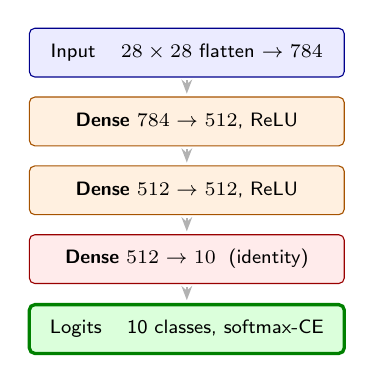
\begin{tikzpicture}[
  >={Stealth[length=1.8mm]},
  every node/.style={font=\sffamily\scriptsize},
  col/.style    = {align=center, rounded corners=2pt, inner sep=2pt, minimum height=0.62cm, minimum width=4.0cm},
  io/.style     = {col, draw=blue!55!black,   fill=blue!8},
  dense/.style  = {col, draw=orange!65!black, fill=orange!12},
  head/.style   = {col, draw=red!60!black,    fill=red!8},
  logits/.style = {col, draw=green!50!black,  fill=green!14, very thick},
  arr/.style    = {->, thick, gray!60, shorten >=1pt, shorten <=1pt},
]
  % Vertical layer column: input at top -> logits at bottom.
  \node[io]                           (input) {Input \;\; $28\times28$ flatten $\to 784$};
  \node[dense, below=0.24cm of input] (d1)    {\textbf{Dense} $784\to512$, ReLU};
  \node[dense, below=0.24cm of d1]    (d2)    {\textbf{Dense} $512\to512$, ReLU};
  \node[head, below=0.24cm of d2]     (d3)    {\textbf{Dense} $512\to10$ \;(identity)};
  \node[logits, below=0.24cm of d3]   (out)   {Logits \;\; 10 classes, softmax-CE};
  \foreach \a/\b in {input/d1, d1/d2, d2/d3, d3/out}
     \draw[arr] (\a) -- (\b);
\end{tikzpicture}
\end{center}

Three dense layers stacked with ReLU non-linearities between them:
$784 \to 512 \to 512 \to 10$. First layer ingests the flattened
image. The two hidden layers let the network learn nonlinear
features. The final layer maps to 10-dimensional logits, one per
digit class.

\subsection*{The verified spec and program}

The network above is a \texttt{VerifiedNetSpec}, the same object type
Chapter~\ref{chap:tensor} used for the linear model, now with two hidden
layers and ReLU between them:

\begin{verbatim}
def mlpVerified : VerifiedNetSpec where
  name     := "MNIST-MLP"
  slug     := "mlp"
  inC      := 1
  imageH   := 28
  imageW   := 28
  nClasses := 10
  data     := .mnist
  layers   := [.dense 784 512, .relu,
               .dense 512 512, .relu,
               .dense 512 10]
\end{verbatim}

Five entries where Chapter~\ref{chap:tensor} had one, and nothing else
about the type changes. The \texttt{slug} binds the spec to
\texttt{verified\_mlir/mlp\_train\_step.mlir} and
\texttt{verified\_mlir/mlp\_fwd.mlir}, and
\texttt{Proofs.MlpRender.mlpTrainStepFaithfulV} is what emits the train
step.

\paragraph{What \texttt{.relu} contributes.} Nothing:

\begin{verbatim}
  | relu => #[]
\end{verbatim}

\noindent ReLU carries no parameters, so its \texttt{toSpecs} arm is the
empty array and the five-entry \texttt{layers} list above still yields
six tensors --- three weight matrices and three biases, the
\texttt{6 params, 669706 floats} the run reported. A layer with no state
is still a layer: it holds a position in the list because the
\emph{render} needs it in order, not because the optimizer does.

The tie back to the proofs has the same shape as before. In
\texttt{LeanMlir/Proofs/Foundation/SpecVJP.lean}:

\begin{verbatim}
noncomputable def mlpVerified_has_vjp (W0 b0 W1 b1 W2 b2) :
    HasVJP (denoteMLP mlpVerified.layers W0 b0 W1 b1 W2 b2) := ...
\end{verbatim}

Again the VJP is proved for the denotation of the spec's own
\texttt{layers} field, and that is the field the trainer reads to build
its graph. The whole program is short enough to print:

\begin{verbatim}
import LeanMlir.VerifiedNets

def mlpConfig : VerifiedConfig where
  epochs    := 12
  batchSize := 128

def main (argv : List String) : IO Unit :=
  mlpVerified.train mlpConfig (argv.head?.getD "data")
\end{verbatim}

That is \texttt{apps/mnist/MainMnistMlpVerified.lean}. The only
difference from Chapter~\ref{chap:tensor}'s driver is \texttt{.train} in
place of \texttt{.trainLinear}, because the MLP carries six parameter
tensors packed together rather than a separate \texttt{W0} and
\texttt{b0}.

XLA compiles that train step in about 5.4 seconds and the forward in
about 40 milliseconds. The train step takes roughly seven times as long
to compile as Chapter~\ref{chap:tensor}'s, which is the cost of six
parameter tensors and two ReLU subgradients rather than one dense layer.

\subsection*{Results}

The run in \S\ref{sec:mlp_runit} is the result. Its per-epoch training
loss, on a log scale:

\begin{center}
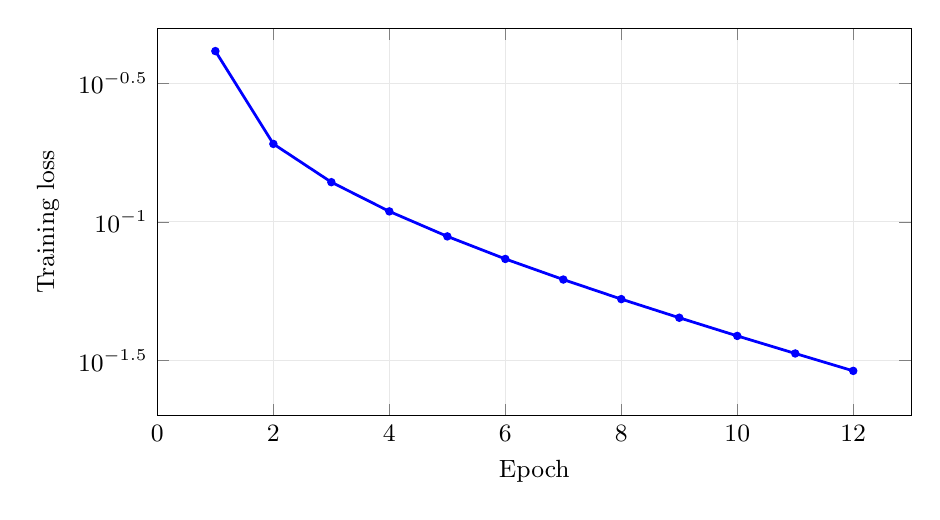
\begin{tikzpicture}
\begin{axis}[
    width=0.92\linewidth, height=6.5cm,
    xlabel={Epoch}, ylabel={Training loss},
    ymode=log,
    xmin=0, xmax=13, ymin=0.02, ymax=0.5,
    xtick={0,2,4,6,8,10,12},
    grid=major, grid style={gray!18},
    tick label style={font=\small},
    label style={font=\small},
    every axis plot/.append style={line width=1pt, mark size=1pt},
]
\addplot[blue, mark=*, mark options={fill=blue}] coordinates {
(1,0.413492) (2,0.191197) (3,0.139092) (4,0.109095) (5,0.088633) (6,0.073492) (7,0.061921) (8,0.052623) (9,0.045073) (10,0.038765) (11,0.033494) (12,0.028984)
};
\end{axis}
\end{tikzpicture}
\end{center}

\noindent MNIST MLP ($784{\to}512{\to}512{\to}10$), SGD~0.1, 12 epochs,
log-scale mean training loss per epoch
(\texttt{runs/2026-08-11-mlp-verified-xla-cuda/}). The loss falls
$14\times$ across the run, and test accuracy ends at 97.83\%.

Both numbers come off the same binary this chapter's theorems describe.
An earlier edition reported 98.57\% here, measured with an unverified
ablation runner that shared the architecture but not the proof-rendered
graph, and that runner was kept because it was the only thing that
printed a loss. The verified train step now returns one, so the second
program is gone.

\section{Return on width}

The $512{\to}512$ hidden size is a convention, not a measurement. Because
the verified renderer is parametric in the layer dimensions, so the same
\texttt{mlp\_has\_vjp} theorem covers every width, being polymorphic in
$d_0,d_1,d_2,d_3$ carry through, we can sweep the hidden width and train each point on
its own proof-rendered StableHLO. The \texttt{mnist-mlp-grid} driver does
exactly this: it renders $784{\to}d{\to}d{\to}10$ from the faithful emitter
and trains it end to end. Sweeping $d$ over the powers of two from 8 to 4096
(each 12-epoch SGD, on the GPU) gives the accuracy-vs-width curve below.

\begin{center}
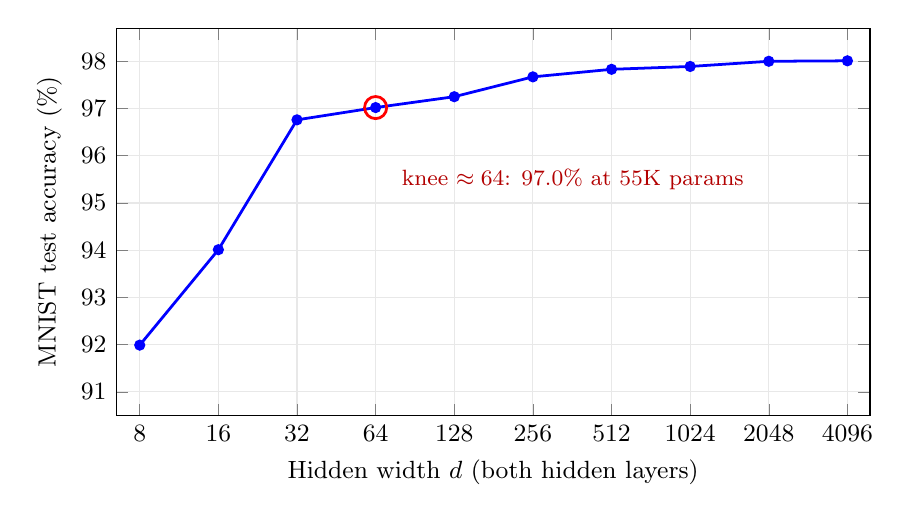
\begin{tikzpicture}
\begin{axis}[
    width=0.92\linewidth, height=6.5cm,
    xlabel={Hidden width $d$ (both hidden layers)},
    ylabel={MNIST test accuracy (\%)},
    xmode=log, log basis x=2,
    xmin=6.5, xmax=5000, ymin=90.5, ymax=98.7,
    xtick={8,16,32,64,128,256,512,1024,2048,4096},
    xticklabels={8,16,32,64,128,256,512,1024,2048,4096},
    ytick={91,92,93,94,95,96,97,98},
    grid=major, grid style={gray!18},
    tick label style={font=\small},
    label style={font=\small},
    every axis plot/.append style={line width=1pt, mark size=1.5pt},
]
\addplot[blue, mark=*, mark options={fill=blue}] coordinates {
(8,91.99) (16,94.01) (32,96.76) (64,97.02) (128,97.25) (256,97.67) (512,97.83) (1024,97.89) (2048,98.00) (4096,98.01)
};
\addplot[only marks, mark=o, mark size=4pt, red, line width=1pt, forget plot] coordinates {(64,97.02)};
\node[anchor=west, font=\footnotesize, red!70!black] at (axis cs:74,95.5)
  {knee $\approx 64$: 97.0\% at 55K params};
\end{axis}
\end{tikzpicture}
\end{center}

\noindent Return on width for the verified MNIST MLP
($784{\to}d{\to}d{\to}10$): test accuracy versus hidden width $d$ (log
scale), 12-epoch SGD on the proof-rendered StableHLO
(\texttt{runs/mlp\_grid\_results\_xla.tsv}). The curve flattens hard after
$\sim$64 neurons: widening $8{\to}64$ buys $+5.0$ points, but $64{\to}4096$
at $64\times$ the width and $364\times$ the parameters, buys only $+1.0$.
A $32{\to}32$ MLP already reaches 96.8\% at 27K parameters, $755\times$
smaller than the $4096{\to}4096$ net (98.0\%). The canonical
$512{\to}512$ sits comfortably on the plateau, and anything past it is paying
for the third decimal place. Off the diagonal the story is capacity
rather than failure. A $784{\to}8{\to}4096{\to}10$ net reaches 93.1\%,
and at three initialization seeds it lands between 93.1\% and 93.7\%.
That is only about a point above what the $8{\to}8$ net manages on its
own (92.0\%). The 8-unit layer is a bottleneck, and width behind it
cannot recover signal that the narrow layer already discarded.

\section{MLIR: Dense}

\noindent\textbf{What is already proven.} \texttt{mlpForward} is the
three-dense-layer network, and \texttt{mlp\_has\_vjp\_at} proves its
reverse-mode derivative (the vector--Jacobian product) by chaining the
per-layer chain rule \texttt{vjp\_comp\_at}. The parameter gradients are
pinned by \texttt{dense\_weight\_grad\_correct} and
\texttt{dense\_bias\_grad\_correct}, and the loss gradient by
\texttt{softmaxCE\_grad}. So \emph{what} the gradient is, is not in
question.

\medskip\noindent\textbf{The gap and how we close it.} The emitted
backward is a value of a Lean datatype, \texttt{Back}, with a denotation
$[\![\cdot]\!]$ into the proofs' own vector type. For the MLP the graph is
\[
  \texttt{emitMlpBack}
  = \texttt{dotGeneral}\,W_0 \circ \texttt{selectPos}\,p_0
    \circ \texttt{dotGeneral}\,W_1 \circ \texttt{selectPos}\,p_1
    \circ \texttt{dotGeneral}\,W_2,
\]
rooted at the incoming cotangent, with
$[\![\texttt{dotGeneral}\,W]\!] = \texttt{Mat.mulVec}\,W$ and
$[\![\texttt{selectPos}\,p]\!] = (v \mapsto \text{if } p>0 \text{ then }
v \text{ else } 0)$, and the bridge theorem
\[
  \texttt{mlp\_whole\_bridge}:\quad
  [\![\texttt{emitMlpBack}]\!](dy)
  = \texttt{mlp\_has\_vjp\_at}.\mathrm{backward}(dy)
\]
says the denotation of that graph is the proven derivative. The forward,
the loss cotangent, and the parameter gradients are covered the same way.
The printer walks the graph and emits one \texttt{stablehlo} op per node:

Here is exactly what the printer emits for that graph, with nothing
hand-written, one \texttt{stablehlo} op per IR node (default
\texttt{precision} attributes elided for the page):

\begin{verbatim}
func.func @mlp_back(%dy: tensor<2x2xf32>, %W0: tensor<4x3xf32>,
    %W1: tensor<3x3xf32>, %W2: tensor<3x2xf32>,
    %p0: tensor<2x3xf32>, %p1: tensor<2x3xf32>) -> tensor<2x4xf32> {
  %bk0 = stablehlo.dot_general %dy, %W2, contracting_dims = [1] x [1]
           : (tensor<2x2xf32>, tensor<3x2xf32>) -> tensor<2x3xf32>
  %bk1 = stablehlo.constant dense<0.0> : tensor<2x3xf32>
  %bk2 = stablehlo.compare GT, %p1, %bk1
           : (tensor<2x3xf32>, tensor<2x3xf32>) -> tensor<2x3xi1>
  %bk3 = stablehlo.select %bk2, %bk0, %bk1
           : tensor<2x3xi1>, tensor<2x3xf32>
  %bk4 = stablehlo.dot_general %bk3, %W1, contracting_dims = [1] x [1]
           : (tensor<2x3xf32>, tensor<3x3xf32>) -> tensor<2x3xf32>
  %bk5 = stablehlo.constant dense<0.0> : tensor<2x3xf32>
  %bk6 = stablehlo.compare GT, %p0, %bk5
           : (tensor<2x3xf32>, tensor<2x3xf32>) -> tensor<2x3xi1>
  %bk7 = stablehlo.select %bk6, %bk4, %bk5
           : tensor<2x3xi1>, tensor<2x3xf32>
  %bk8 = stablehlo.dot_general %bk7, %W0, contracting_dims = [1] x [1]
           : (tensor<2x3xf32>, tensor<4x3xf32>) -> tensor<2x4xf32>
  return %bk8 : tensor<2x4xf32>
}
\end{verbatim}

\noindent Read it against the graph: each \texttt{dot\_general}
(\texttt{\%bk0}, \texttt{\%bk4}, \texttt{\%bk8}) is a
\texttt{dotGeneral}\,$W$ node, whose denotation is
$\texttt{Mat.mulVec}\,W$. Each \texttt{compare GT} + \texttt{select}
pair (\texttt{\%bk2}/\texttt{\%bk3}, \texttt{\%bk6}/\texttt{\%bk7}) is a
\texttt{selectPos}\,$p$ node, which is the ReLU subgradient. The bridge
theorem is precisely the claim that this text computes
\texttt{mlp\_has\_vjp\_at}'s backward.

\medskip\noindent\textbf{Caveats.}
\begin{itemize}
  \item \textbf{ReLU is a smooth-point bridge.} Where a pre-activation is
    exactly zero ReLU has no derivative. The emitted \texttt{compare GT 0}
    sends that case to $0$, and the bridge is permitted to fail on that
    measure-zero set.
  \item \textbf{Representative scale.} Shown small. The trained net is
    $784{\to}512{\to}512{\to}10$.
  \item \textbf{Trusted surface.} The printer's faithfulness and the
    lowerer's translation are tested rather than proved. Rounding
    $\approx \mathbb{R}$ is no longer on this list: it is a theorem layer
    over an arbitrary rounding model (\S~\ref{sec:precision}), conditional on
    two measured constants rather than assumed outright. Appendix~\ref{sec:verified_codegen} has the
    full accounting.
\end{itemize}

\chapter{MNIST: 2D CNN}
\label{chap:cnn}

\prosesection{The MLP wastes information, and we can do better}

Chapter \ref{chap:mlp}'s MLP recognized digits by flattening every
28$\times$28 image into a 784-dim vector and feeding it through
three dense layers. It worked. But it worked by ignoring something
the data was telling us. Pixel \((5, 5)\) and pixel \((5, 6)\) are
neighbors: they were next to each other on the page where the digit
was drawn. Pixel \((5, 5)\) and pixel \((23, 14)\) are not. The
dense layer has no idea. It treats every input coordinate as an
independent feature. Its weight matrix has no notion that some
pairs of pixels are geometrically close. A trained MLP eventually
learns to compensate, but it has to learn it from the data, with
the data, by paying the full price for each unrelated feature pair.

A handwritten ``5'' drawn in the top-left of the image and the
same ``5'' drawn in the bottom-right are the same digit. The MLP
sees them as completely unrelated vectors. It can be trained to
classify both, but each is its own learning problem, and nothing it
learned about one transfers to the other for free.

Convolutional networks fix this by building three priors directly
into the architecture, priors that the data has but the MLP
threw away.

\section{Run it first}
\label{sec:cnn_runit}

Before any of the math, train the thing. Four commands and about a
minute of GPU time:

\begin{verbatim}
lake exe cache get                            # Mathlib oleans, ~30 s
./download_mnist.sh                           # ~11 MB
lake build mnist-cnn-verified
./.lake/build/bin/mnist-cnn-verified data
\end{verbatim}

On one RTX 4060 Ti (CUDA 12.9), from
\texttt{runs/2026-08-11-cnn-verified-xla-cuda/}. XLA's startup banner is
removed and one long line is wrapped:

\begin{verbatim}
[pjrt_ffi] XLA backend: PJRT 0.112, 1 device(s)
[pjrt_ffi] compiled verified_mlir/cnn_train_step.mlir
             (@cnn_train_step, 11 outputs, 1 replica) in 2490 ms
[pjrt_ffi] compiled verified_mlir/cnn_fwd.mlir
             (@cnn_fwd, 1 outputs, 1 replica) in 383 ms
MNIST-CNN via the VERIFIED renderer (conv→conv→pool→512→512→10) → XLA/PJRT → GPU
  xla/pjrt verified_mlir/cnn_train_step.mlir
  xla/pjrt verified_mlir/cnn_fwd.mlir
  train 60000, test 10000; bs 128, MNIST-CNN (10 params, 3489130 floats),
    mean-loss SGD lr=0.100000, He init
  epoch 1: loss = 0.348858, test_acc = 9465/10000 = 94.650000% (5922ms)
  epoch 2: loss = 0.094931, test_acc = 9740/10000 = 97.400000% (6063ms)
  epoch 3: loss = 0.056737, test_acc = 9807/10000 = 98.070000% (5795ms)
  epoch 4: loss = 0.038233, test_acc = 9829/10000 = 98.290000% (4608ms)
  epoch 5: loss = 0.026337, test_acc = 9844/10000 = 98.440000% (5533ms)
  epoch 6: loss = 0.017761, test_acc = 9834/10000 = 98.340000% (5663ms)
  epoch 7: loss = 0.015211, test_acc = 9830/10000 = 98.300000% (4770ms)
  epoch 8: loss = 0.009691, test_acc = 9869/10000 = 98.690000% (4957ms)
  epoch 9: loss = 0.035910, test_acc = 9836/10000 = 98.360000% (4486ms)
  epoch 10: loss = 0.014582, test_acc = 9875/10000 = 98.750000% (4618ms)
done (trained MNIST-CNN via the proof-rendered StableHLO).
\end{verbatim}

Ten epochs at about 5 seconds each, and 98.75\% on the full
10,000-image test set. Two convolutions in front of
Chapter~\ref{chap:mlp}'s classifier buy 0.9 points over the MLP's
97.83\%, and they do it with 3.5M parameters against the MLP's 670K.

The claim survives convolution. That run did not execute a
reimplementation of the network this chapter describes. It executed
\texttt{verified\_mlir/cnn\_train\_step.mlir}, which is the text
\texttt{Proofs.StableHLO.cnnTrainStepFaithfulV} emits, and
\texttt{CnnFaithfulPoC} proves that each of the ten parameter updates
denotes the certified softmax cross-entropy loss-descent step derived
from the Mathlib \(\fderiv\) math. The module carries one line that is
not \texttt{pretty} of a proven node, the trailing \texttt{\%loss} scalar,
and it says so in its own comment. It feeds the printed loss above and
nothing else. Both convolutions, the max pool, the
three dense layers, and the SGD update are all proof-backed operations.

\prosesection{Three properties baked into a convolution}

\begin{enumerate}
\item \textbf{Locality.} Each output value depends on only a small
  neighborhood of inputs. A convolution with a \(3 \times 3\) kernel
  computes each output pixel as a weighted sum of its 9 neighbors.
  Faraway pixels do not enter directly. The network only learns to
  combine them later, by stacking convolutions and letting receptive
  fields grow.

\item \textbf{Translation invariance.} The same weights are applied
  at every spatial position. A feature detector that recognizes the
  bottom-left curve of a ``5'' uses the same parameters whether the
  curve appears at row 5 or row 25. The architecture imposes the
  symmetry, and the data does not have to teach it.

\item \textbf{Parameter sharing.} A \(3 \times 3 \times 1 \to 32\)
  convolution has \(3 \times 3 \times 1 \times 32 + 32 = 320\)
  parameters total, regardless of image size. The matching
  fully-connected layer on a 28$\times$28 image would have
  \(28^2 \times 28^2 \times 32 \approx 20\) million. The
  convolution gets the same expressive power with four orders of
  magnitude fewer parameters because it reuses them.
\end{enumerate}

Concretely, a convolution computes

\[
y_{c_{\text{out}},\, i,\, j}
\;=\;
\sum_{c_{\text{in}},\, k_h,\, k_w}\,
W_{c_{\text{out}},\, c_{\text{in}},\, k_h,\, k_w}
\cdot
x_{c_{\text{in}},\, i + k_h,\, j + k_w}
\;+\;
b_{c_{\text{out}}}.
\]

Each output cell is a small dot product between the kernel \(W\)
and a window of the input. The sum is over a tiny \(3 \times 3\)
spatial region and over input channels, usually a handful of
terms rather than the 784 a dense layer touches.

\prosesection{The Jacobian is sparse and structured}

The Jacobian of a convolution looks like a giant matrix, but it
isn't a generic giant matrix. It is mostly zeros. Specifically,
\(\partial y_{c_{\text{out}}, i, j} / \partial x_{c_{\text{in}}, i', j'}\)
is zero unless \((i', j')\) falls inside the kernel window centered
at \((i, j)\). When it does, the entry is just the corresponding
weight \(W_{c_{\text{out}}, c_{\text{in}}, k_h, k_w}\).

So a convolution is a linear map, like a dense layer, but its
Jacobian is highly structured: each row has only \(k^2 \times C_{\text{in}}\)
nonzero entries, and those entries are reused across many rows
because the same kernel is used at every spatial position. The
forward picture from Chapter \ref{chap:mlp} ``the Jacobian of a
linear map is the linear map'' still holds. The Jacobian is just
written in a different basis: instead of one big dense matrix it
is a list of kernel weights plus a rule for where each one lives.

\prosesection{The backward of a convolution is another convolution}

We want \(dx\), the way a small jiggle in each input pixel changes
the loss, given an upstream \(dy\). Plugging into the Jacobian above and grinding through the
algebra, the answer is:

\[
dx_{c_{\text{in}}, i', j'}
\;=\;
\sum_{c_{\text{out}},\, k_h,\, k_w}\,
W_{c_{\text{out}},\, c_{\text{in}},\, k_h,\, k_w}
\cdot
dy_{c_{\text{out}},\, i' - k_h,\, j' - k_w}.
\]

That is itself a convolution. Specifically, it is a convolution
of the upstream gradient \(dy\) against the same kernel \(W\),
but with the spatial axes \emph{reversed} and the input/output
channel axes \emph{swapped}, which is a ``transposed convolution''.
The backward of a CNN block reuses the same kind of operation as the
forward, and no new primitive is needed.

The weight gradient \(dW\) similarly works out to a convolution,
this time of the saved input \(x\) against the upstream gradient
\(dy\) (the ``transpose trick''). The bias gradient \(db\) is just
\(dy\) summed over spatial positions per channel. Theorems
\ref{ax:conv2d_has_vjp3}, \ref{ax:conv2d_weight_grad_has_vjp}, and
\ref{ax:conv2d_bias_grad_has_vjp} formalize each of these.

\prosesection{Max pooling: the winner gets the gradient}

The other new primitive in this chapter is max pooling. A
\(2 \times 2\) max pool collapses each \(2 \times 2\) block of the
input into a single output value: the max of the four. It has no
parameters, and its purpose is to halve the spatial resolution while
keeping the strongest local response.

The Jacobian of \(\max\) is degenerate. At a generic point, only one
of the four inputs is the maximum, and the output's slope is \(1\)
with respect to that one input and \(0\) with respect to the
other three. ``Jiggle the max'' moves the output, and ``jiggle a
non-max'' does nothing. So the backward of max pool routes the
upstream gradient back to whichever input was the winner in each
window, and zeros out the rest. At ties the codegen breaks
deterministically (same convention as ReLU's kink). Definition
\ref{ax:maxPool2_has_vjp3} states this formally.

\prosesection{The rest of the network is Chapter 2}

After two convolutions and a max pool, the feature map is
\(14 \times 14 \times 32\). At that point we \texttt{flatten} the
\(14 \cdot 14 \cdot 32 = 6272\)-dim feature vector and feed it into
the same three-dense-layer head from Chapter \ref{chap:mlp},
ending in 10-class logits. The backward through the dense head and
the softmax-CE loss is exactly the calculation we did in the
previous chapter, and we do not re-prove it here. The composition rule
from Chapter \ref{chap:tensor} guarantees that the full network's
VJP is just the per-layer VJPs strung together in reverse order:
softmax-CE backward, dense backward $\times 3$, flatten backward,
max-pool backward, conv2d backward $\times 2$. Each piece is its
own theorem, and together they form a working trainer for MNIST that
respects the image's 2-D structure.

\section{The theorems}

\begin{definition}[Conv2d forward]
  \label{ax:conv2d}
  \lean{Proofs.conv2d}
  \leanok
  Concrete \(\sum_{c,kh,kw}\) cross-correlation with SAME padding.
  Codegen emits \texttt{stablehlo.convolution}; proofs reason about it
  via the explicit definition.
\end{definition}

\begin{definition}[3D VJP record]
  \label{def:hasvjp3}
  \lean{Proofs.HasVJP3}
  \leanok
  \uses{ax:pdiv, def:hasvjp}
  The rank-3 analogue of Definition~\ref{def:hasvjp}. For
  \(f : \mathrm{Tensor3} \to \mathrm{Tensor3}\), define
  \(\pdiv_3 f\, x\, (c_i, h_i, w_i)\, (c_o, h_o, w_o)\) as \(\pdiv\)
  of the flattened map
  \(v \mapsto \mathrm{flatten}\bigl(f(\mathrm{unflatten}\, v)\bigr)\)
  with both indices decoded through the
  \((c, h, w) \leftrightarrow \text{flat}\) bijection. Then
  \(\HasVJPthree\, f\) bundles a backward function \(B\) with: for all
  \(x\), \(dy\), \((c_i, h_i, w_i)\),
  \[
    B(x, dy)_{c_i h_i w_i}
      = \sum_{c_o, h_o, w_o}
        \pdiv_3 f\, x\, (c_i, h_i, w_i)\, (c_o, h_o, w_o)
        \cdot dy_{c_o h_o w_o}.
  \]
\end{definition}

\begin{theorem}[Conv2d input VJP]
  \label{ax:conv2d_has_vjp3}
  \lean{Proofs.conv2d_has_vjp3}
  \leanok
  \uses{ax:conv2d, ax:pdiv_add, ax:pdiv_const, ax:pdiv_mul, thm:pdiv_finset_sum, ax:pdiv_reindex, def:hasvjp3}
  \(\HasVJPthree\, \bigl(\mathrm{conv2d}(W, b)\bigr)\): the input
  backward of a convolution is the reversed-kernel convolution.
  No hypotheses: conv2d is affine in its input.
\end{theorem}

\begin{proof}
\leanok
\emph{Sketch: same split--distribute--product-rule--collapse skeleton
as the dense Jacobians (Theorems~\ref{ax:pdiv_dense},
\ref{ax:pdiv_dense_W}), with two convolution-specific twists: the
finite-sum rule fires three times (over \(c, k_h, k_w\)), and the
product rule's variable factor is a \emph{pad-conditional} projection
--- a case split on the SAME-padding condition decides between a
coordinate projection and the zero function.}
\begin{enumerate}
  \item Define \(B(x, dy)_{c_i h_i w_i} :=
    \sum_{c_o, h_o, w_o} [\text{pad-valid}]\;
      W_{c_o, c_i, \hat{k}_h, \hat{k}_w} \cdot dy_{c_o h_o w_o}\),
    where \(\hat{k}_h = h_i + p_H - h_o\),
    \(\hat{k}_w = w_i + p_W - w_o\) are the reconstructed kernel
    offsets and \([\text{pad-valid}]\) requires them to lie in
    \([0, k_H) \times [0, k_W)\). Under the substitution
    \(k_h \leftrightarrow k_H - 1 - k_h\) this is the reversed-kernel,
    channel-swapped convolution of \(dy\) against \(W\) that the MLIR
    backward emits (\texttt{transpose} + \texttt{reverse} +
    \texttt{convolution}).
  \item \Suffices{} for all \(x\), \(dy\), \((c_i, h_i, w_i)\):
    \(B(x, dy)_{c_i h_i w_i}\) equals the \(\pdiv_3\) triple sum.
    \pf{Definition~\ref{def:hasvjp3}, with \(B\) as the candidate
    backward function.}
  \item The flattened forward
    \(v \mapsto \mathrm{flatten}\bigl(\mathrm{conv2d}(W, b)\,
      (\mathrm{unflatten}\, v)\bigr)\)
    is affine in \(v\): a constant bias term plus
    \(\sum_{c, k_h, k_w} W_{o(\mathrm{idx}), c, k_h, k_w} \cdot
      (\text{pad-conditional projection of } v)\).
    \pf{Unfold \(\mathrm{conv2d}\) and \(\mathrm{flatten}\);
    definitional (Definition~\ref{ax:conv2d}).}
  \item Per-index Jacobian: for every flat \(\mathrm{idx_{in}}\),
    \(\mathrm{idx_{out}}\),
    \(\pdiv\)(flattened forward) \(=
      \sum_{c, k_h, k_w} W_{o(\mathrm{idx_{out}}), c, k_h, k_w} \cdot
      [\text{pad-valid} \wedge \mathrm{idx_{in}} =
        \text{encoded input position}]\).
    \pf{By 3: sum rule + constant rule
    (Theorems~\ref{ax:pdiv_add}, \ref{ax:pdiv_const}) drop the bias;
    the finite-sum rule (Theorem~\ref{thm:pdiv_finset_sum}) fires
    three times over \((c, k_h, k_w)\); per summand the product rule
    (Theorem~\ref{ax:pdiv_mul}) applies with the \(W\)-factor
    constant, and a case split on the pad condition leaves either a
    coordinate projection --- a reindex, whose Jacobian is the
    Kronecker indicator (Theorem~\ref{ax:pdiv_reindex}) --- or the
    zero function (Theorem~\ref{ax:pdiv_const}).}
  \item Contract 4 with \(dy\) and collapse: re-index the sum over
    flat \(\mathrm{idx_{out}}\) to \((c_o, h_o, w_o)\); for each
    fixed output position the triple sum over \((c, k_h, k_w)\)
    collapses by three \texttt{Finset.sum\_eq\_single} applications
    at \(c = c_i\), \(k_h = \hat{k}_h\), \(k_w = \hat{k}_w\).
    \pf{The indicator in 4 is nonzero for exactly that one summand.}
  \item \Qed{}
    \pf{What remains after 5 is exactly \(B(x, dy)_{c_i h_i w_i}\)
    from 1; with 2 this is the goal.}
\end{enumerate}
\end{proof}

\begin{theorem}[Conv2d weight VJP]
  \label{ax:conv2d_weight_grad_has_vjp}
  \lean{Proofs.conv2d_weight_grad_has_vjp}
  \leanok
  \uses{ax:conv2d, ax:pdiv_add, ax:pdiv_const, ax:pdiv_mul, thm:pdiv_finset_sum, ax:pdiv_reindex, def:hasvjp}
  The transpose-trick formula. As with the dense weight
  Jacobian (Theorem~\ref{ax:pdiv_dense_W}), differentiate in the
  \emph{flattened} kernel: let
  \(F(v) := \mathrm{flatten}\bigl(\mathrm{conv2d}
    (\mathrm{unflatten}\, v,\, b)\, x\bigr)\)
  for \(v \in \Vect{o_c \cdot i_c \cdot k_H \cdot k_W}\).
  \Prove{} \(\HasVJP\, F\), with backward
  \(dW_{o, c, k_h, k_w} = \sum_{h_i, w_i}
    [\text{pad-valid}]\; x_{c,\, h_i + k_h - p_H,\, w_i + k_w - p_W}
    \cdot dy_{o, h_i, w_i}\)
  --- a convolution of the saved input against the upstream gradient.
\end{theorem}

\begin{proof}
\leanok
\emph{Sketch: the dual of Theorem~\ref{ax:conv2d_has_vjp3} --- the
same affine decomposition, but now \(v\) (the kernel) sits in the
reindex factor and the saved input \(x\) is the constant.}
\begin{enumerate}
  \item Define \(B(v, dy)_{\mathrm{idx}}\), decoding
    \(\mathrm{idx} \leftrightarrow (o', c', k_h', k_w')\), as
    \(\sum_{h_i, w_i} (\text{pad-conditional } x \text{ value at }
      (c', h_i + k_h' - p_H, w_i + k_w' - p_W))
      \cdot dy_{\mathrm{flat}(o', h_i, w_i)}\).
  \item \Suffices{} for all \(v\), \(dy\), \(\mathrm{idx}\):
    \(B(v, dy)_{\mathrm{idx}} = \sum_{\mathrm{idx_{out}}}
      \pdiv F\, v\, \mathrm{idx}\, \mathrm{idx_{out}} \cdot
      dy_{\mathrm{idx_{out}}}\).
    \pf{Definition~\ref{def:hasvjp}, with \(B\) as the candidate
    backward function.}
  \item \(F\) is affine in \(v\): constant bias plus
    \(\sum_{c, k_h, k_w} v_{\varphi(o(\mathrm{idx_{out}}), c, k_h, k_w)}
      \cdot (\text{pad-conditional } x \text{ term})\), where
    \(\varphi\) is the kernel-index bijection
    (\texttt{Kernel4.flatten}).
    \pf{Unfold \(\mathrm{conv2d}\) and the flattens; definitional
    (Definition~\ref{ax:conv2d}).}
  \item Per-index Jacobian:
    \(\pdiv F\, v\, \mathrm{idx}\, \mathrm{idx_{out}}
      = \sum_{c, k_h, k_w}
        [\mathrm{idx} = \varphi(o(\mathrm{idx_{out}}), c, k_h, k_w)]
        \cdot (\text{pad-conditional } x \text{ term})\).
    \pf{By 3: sum rule + constant rule (Theorems~\ref{ax:pdiv_add},
    \ref{ax:pdiv_const}) drop the bias; finite-sum rule
    (Theorem~\ref{thm:pdiv_finset_sum}) \(\times 3\); product rule
    (Theorem~\ref{ax:pdiv_mul}) with the \(x\)-factor constant and
    the \(v\)-factor a reindex through \(\varphi\), whose Jacobian is
    the Kronecker indicator (Theorem~\ref{ax:pdiv_reindex}).}
  \item Contract 4 with \(dy\) and collapse: the \((c, k_h, k_w)\)
    sum collapses on \(\mathrm{idx}\)'s decode
    \((c', k_h', k_w')\) by injectivity of \(\varphi\)
    (\texttt{Finset.sum\_eq\_single} \(\times 3\)); re-index
    \(\mathrm{idx_{out}}\) to \((o, h_i, w_i)\) and collapse the
    channel sum at \(o = o'\).
    \pf{The indicator forces \(o = o'\); the spatial sums survive.}
  \item \Qed{}
    \pf{What remains after 5 is exactly \(B(v, dy)_{\mathrm{idx}}\)
    from 1; with 2 this is the goal.}
\end{enumerate}
\end{proof}

\begin{theorem}[Conv2d bias VJP]
  \label{ax:conv2d_bias_grad_has_vjp}
  \lean{Proofs.conv2d_bias_grad_has_vjp}
  \leanok
  \uses{ax:conv2d, ax:pdiv_add, ax:pdiv_const, ax:pdiv_reindex, def:hasvjp}
  Sum the cotangent over spatial dims per channel.
  \Prove{} \(\HasVJP\, \bigl(b \mapsto \mathrm{flatten}
    (\mathrm{conv2d}(W, b)\, x)\bigr)\), with backward
  \(db_o = \sum_{h_i, w_i} dy_{\mathrm{flat}(o, h_i, w_i)}\).
\end{theorem}

\begin{proof}
\leanok
\begin{enumerate}
  \item Define \(B(b, dy)_o := \sum_{h_i, w_i}
    dy_{\mathrm{flat}(o, h_i, w_i)}\).
  \item \Suffices{} for all \(b\), \(dy\), \(o\):
    \(B(b, dy)_o = \sum_{\mathrm{idx}}
      \pdiv\bigl(b' \mapsto \mathrm{flatten}(\mathrm{conv2d}(W, b')\, x)\bigr)\,
      b\, o\, \mathrm{idx} \cdot dy_{\mathrm{idx}}\).
    \pf{Definition~\ref{def:hasvjp}, with \(B\) as the candidate
    backward function.}
  \item As a function of \(b\), the flattened forward is
    \((\text{channel reindex of } b) + (\text{$W\!,x$ term constant
    in } b)\), so
    \(\pdiv = \delta_{o,\, \mathrm{chan}(\mathrm{idx})}\).
    \pf{Sum rule (Theorem~\ref{ax:pdiv_add}), reindex Jacobian
    (Theorem~\ref{ax:pdiv_reindex}) with
    \(\sigma = \mathrm{idx} \mapsto \mathrm{chan}(\mathrm{idx})\),
    constant rule (Theorem~\ref{ax:pdiv_const}).}
  \item \Qed{}
    \pf{Contract 3 with \(dy\): re-index the flat sum to
    \((c, h_i, w_i)\); the Kronecker keeps exactly channel \(o\)'s
    spatial positions (\texttt{Finset.sum\_eq\_single}), leaving
    \(B(b, dy)_o\); with 2 this is the goal.}
\end{enumerate}
\end{proof}

\begin{definition}[MaxPool 2x2 stride 2 forward]
  \label{ax:maxPool2}
  \lean{Proofs.maxPool2}
  \leanok
  Concrete four-way max over 2x2 windows.
\end{definition}

\begin{definition}[MaxPool input VJP]
  \label{ax:maxPool2_has_vjp3}
  \lean{Proofs.maxPool2_has_vjp3}
  \leanok
  \uses{ax:maxPool2}
  \texttt{noncomputable def} over the canonical pdiv-derived
  witness. \texttt{HasVJP.correct} holds by \texttt{rfl}; codegen
  substitutes the standard argmax routing convention at tiebreaks.
\end{definition}

\section{Example: MNIST 2D CNN}
\label{sec:cnn_mnist_example}

The MLP in Chapter~\ref{chap:mlp} crushed MNIST by flattening the
image into a 784-dim vector and throwing dense layers at it. That
works because MNIST is small, but it also throws away \emph{all}
the spatial structure: pixel (5,5) and pixel (5,6) are neighbors,
but the MLP sees no more relationship between them than it does
between pixel (5,5) and pixel (23,14). Convolutions fix that. This
chapter does MNIST again, the same way the Swift for TensorFlow
book's Chapter 1 did it: two plain $3 \times 3$ convs to pull out
local features, a max-pool to collapse the spatial grid, then the
same dense head you already know.

\subsection*{Architecture}

\begin{center}
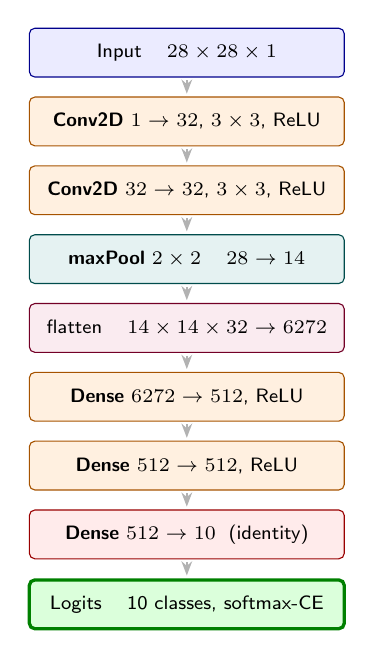
\begin{tikzpicture}[
  >={Stealth[length=1.8mm]},
  every node/.style={font=\sffamily\scriptsize},
  col/.style    = {align=center, rounded corners=2pt, inner sep=2pt, minimum height=0.62cm, minimum width=4.0cm},
  io/.style     = {col, draw=blue!55!black,   fill=blue!8},
  conv/.style   = {col, draw=orange!65!black, fill=orange!12},
  pool/.style   = {col, draw=teal!60!black,   fill=teal!10},
  flat/.style   = {col, draw=purple!60!black, fill=purple!8},
  dense/.style  = {col, draw=orange!65!black, fill=orange!12},
  head/.style   = {col, draw=red!60!black,    fill=red!8},
  logits/.style = {col, draw=green!50!black,  fill=green!14, very thick},
  arr/.style    = {->, thick, gray!60, shorten >=1pt, shorten <=1pt},
]
  % Vertical layer column: input at top -> logits at bottom.
  \node[io]                          (input) {Input \;\; $28\times28\times1$};
  \node[conv, below=0.24cm of input] (c1)    {\textbf{Conv2D} $1\to32$, $3\times3$, ReLU};
  \node[conv, below=0.24cm of c1]    (c2)    {\textbf{Conv2D} $32\to32$, $3\times3$, ReLU};
  \node[pool, below=0.24cm of c2]    (p1)    {\textbf{maxPool} $2\times2$ \;\; $28\to14$};
  \node[flat, below=0.24cm of p1]    (fl)    {flatten \;\; $14\times14\times32 \to 6272$};
  \node[dense, below=0.24cm of fl]   (d1)    {\textbf{Dense} $6272\to512$, ReLU};
  \node[dense, below=0.24cm of d1]   (d2)    {\textbf{Dense} $512\to512$, ReLU};
  \node[head, below=0.24cm of d2]    (d3)    {\textbf{Dense} $512\to10$ \;(identity)};
  \node[logits, below=0.24cm of d3]  (out)   {Logits \;\; 10 classes, softmax-CE};
  \foreach \a/\b in {input/c1, c1/c2, c2/p1, p1/fl, fl/d1, d1/d2, d2/d3, d3/out}
     \draw[arr] (\a) -- (\b);
\end{tikzpicture}
\end{center}

Two convolutions lift the 1-channel grayscale input to 32 channels,
maxPool halves the spatial resolution, then the flattened
$14 \times 14 \times 32 = 6272$ feature vector goes through three
dense layers into 10-class logits. No batch norm yet, because BN shows
up in Chapter~\ref{chap:bn}.

\subsection*{Code: the full training program}

Same format as the MLP chapter. The only thing that changes from
Chapter~\ref{chap:mlp}'s training program is the \texttt{layers} list.
This is the spec \S\ref{sec:cnn_runit} actually ran.

\begin{verbatim}
-- 1
import LeanMlir

-- 2
def cnnVerified : VerifiedNetSpec where
  name     := "MNIST-CNN"
  slug     := "cnn"
  inC      := 1
  imageH   := 28
  imageW   := 28
  nClasses := 10
  data     := .mnist
  layers   := [.conv 1 32 3 1, .relu, .conv 32 32 3 1, .relu, .maxPool 2 2,
               .flatten,
               .dense 6272 512, .relu, .dense 512 512, .relu, .dense 512 10]

-- 3
def cnnConfig : VerifiedConfig where
  epochs    := 10
  batchSize := 128

-- 4
def main (argv : List String) : IO Unit :=
  cnnVerified.train cnnConfig (argv.head?.getD "data")
\end{verbatim}

Walking through the numbered sections:

\textbf{1. The import.} Same as Chapter~\ref{chap:mlp}.

\textbf{2. The architecture.} Eleven entries: two \texttt{.conv}
layers at 32 channels, a \texttt{.maxPool}, a \texttt{.flatten}, three
\texttt{.dense} layers down to 10, and four \texttt{.relu}s between
them. \texttt{.conv ic oc k stride} takes in-channels, out-channels,
kernel size and stride --- no activation argument, because activations
are their own entries here rather than a field on the layer that
precedes them. That is why Chapter~\ref{chap:mlp}'s five-entry list
became eleven and not seven.

The \texttt{.conv2d} backward pass is the theorem from earlier in
this chapter (\S~\ref{ax:conv2d_has_vjp3}): the input VJP is
another convolution, using the kernel reversed along both spatial
axes. The max-pool backward (\S~\ref{ax:maxPool2_has_vjp3}) routes
the gradient to the argmax position in each $2 \times 2$ window.
The dense backward is already proved in
Chapter~\ref{chap:mlp} (\S~\ref{thm:dense_has_vjp}). Adding
convolution to the model introduces no new training-loop code, only
new layer types, which the framework already knows how to compose.

\textbf{3. The training hyperparameters.} Ten epochs at batch 128,
SGD, no regularization and no augmentation. Note what a
\texttt{VerifiedConfig} does \emph{not} carry: the learning rate. It is
baked into \texttt{verified\_mlir/cnn\_train\_step.mlir}, which is
\S\ref{sec:mlp_inside_train}'s point in a second chapter --- the rate is
inside the reach of the proofs, so it cannot be set to one thing and
trained at another. That's the
framework's pitch made concrete: swap the architecture, keep the
trainer. The ablation framework gives you access to the same
variant configs (\texttt{adamOnly}, \texttt{fullRecipe}, etc.)
without any more changes on your side.

\textbf{4. The program entry point.} One line, same as the MLP
chapter. \texttt{cnnVerified.train cnnConfig} replaces
\texttt{mlpVerified.train mlpConfig}. That's the whole diff.

\paragraph{What \texttt{.conv}, \texttt{.maxPool} and \texttt{.flatten}
contribute.} Three more arms on Chapter~\ref{chap:tensor}'s
\texttt{toSpecs}, and only one of them carries parameters:

\begin{verbatim}
  | conv ic oc k _ => #[(#[oc,ic,k,k],0),(#[oc],2)]   -- W, bias
  | maxPool _ _    => #[]
  | flatten        => #[]
\end{verbatim}

\noindent Pooling and flattening are pure reshapes of data, so they have
nothing to initialise --- which is the parameter-list statement of the
same fact the backward passes above make: \texttt{maxPool2}'s VJP routes
gradient without owning any, and \texttt{flatten}'s is a reshape. Fold
the eleven-entry list through those arms and you get the
\texttt{10 params, 3489130 floats} the run printed: two conv kernels and
their biases, three dense matrices and theirs.

\subsection*{Results}

The run in \S\ref{sec:cnn_runit} is the result. Its per-epoch training
loss, against Chapter~\ref{chap:mlp}'s MLP on the same recipe:

\begin{center}
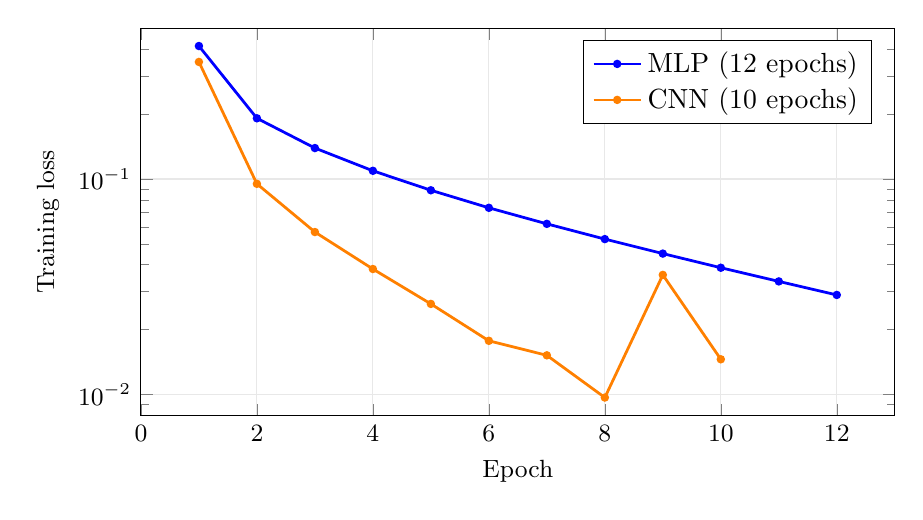
\begin{tikzpicture}
\begin{axis}[
    width=0.92\linewidth, height=6.5cm,
    xlabel={Epoch}, ylabel={Training loss},
    ymode=log,
    xmin=0, xmax=13, ymin=0.008, ymax=0.5,
    xtick={0,2,4,6,8,10,12},
    legend pos=north east,
    legend cell align={left},
    grid=major, grid style={gray!18},
    tick label style={font=\small},
    label style={font=\small},
    every axis plot/.append style={line width=1pt, mark size=1pt},
]
\addplot[blue, mark=*, mark options={fill=blue}] coordinates {
(1,0.413492) (2,0.191197) (3,0.139092) (4,0.109095) (5,0.088633) (6,0.073492) (7,0.061921) (8,0.052623) (9,0.045073) (10,0.038765) (11,0.033494) (12,0.028984)
};
\addlegendentry{MLP (12 epochs)}
\addplot[orange, mark=*, mark options={fill=orange}] coordinates {
(1,0.348858) (2,0.094931) (3,0.056737) (4,0.038233) (5,0.026337) (6,0.017761) (7,0.015211) (8,0.009691) (9,0.035910) (10,0.014582)
};
\addlegendentry{CNN (10 epochs)}
\end{axis}
\end{tikzpicture}
\end{center}

\noindent MNIST, SGD~0.1, log-scale mean training loss per epoch
(\texttt{runs/2026-08-11-\{mlp,cnn\}-verified-xla-cuda/}). The CNN is
below the MLP from the second epoch onward and reaches in 10 epochs a
loss the MLP does not reach in 12. Test accuracy is 98.75\% against the
MLP's 97.83\%. The bump at the CNN's ninth epoch is ordinary SGD at
$\text{lr}=0.1$ rather than a measurement artifact, and the accuracy
trace in \S\ref{sec:cnn_runit} dips at the same epoch.

Both curves come off the binaries these chapters' theorems describe. An
earlier edition plotted an unverified ablation runner here, which shared
the architectures but not the proof-rendered graphs, and reported 98.98\%
against 98.57\%. It was kept because it was the only thing that printed a
loss. The verified train steps now return one.

\subsection*{Why this network is still 99\% dense-head}

At 3{,}489{,}130 total parameters, the no-BN CNN is actually
$\sim$5.2$\times$ \emph{bigger} than the MLP, not smaller. You
might have expected the opposite, because convolutions are supposed
to be parameter-efficient. They are, but the \emph{head} is what's
eating the budget: the flatten of a $14 \times 14 \times 32$ feature
map produces a 6272-dim vector, and the first dense layer
(\texttt{6272 $\to$ 512}) alone is 3{,}211{,}776 parameters. The
entire conv+maxPool backbone is 9{,}568 parameters, which is 0.27\%
of the total.

This is the same ``fat FC head'' pattern you'll see in AlexNet, VGG,
and YOLOv1: a compact convolutional backbone feeding a massive
fully-connected classifier. Historically it drove practitioners
crazy, because the conv layers were the interesting new machinery but
all the weight budget lived in the part nobody had done anything
new with. Every post-2015 vision architecture responded by
replacing the dense head with \texttt{globalAvgPool} followed by a
single small dense, which is why ResNet-18 has $\sim$11M parameters
for 1000-class ImageNet but Chapter~\ref{chap:cnn}'s 10-class MNIST
CNN has 3.5M. We'll see the switch firsthand starting with ResNet
in Chapter~\ref{chap:residual}.

The MLIR character count also tells a story: the CNN emits 21{,}884
chars vs the MLP's 10{,}375, about 2.1$\times$ bigger. Adding
convolutions and maxPool roughly doubles the emitted compute, not
3.5$\times$ the way our \emph{other} (BN-equipped) CNN does. Every
\texttt{.convBn} adds batch-norm normalize and affine ops, and the
plain \texttt{.conv2d} used here keeps the StableHLO much tighter.

\subsection*{The fat head is fat because it can be, not because it must be}

If the dense head holds 99\% of the parameters, the obvious question is how
many of them earn their keep. The parametric renderer answers it directly:
\texttt{mnist-cnn-grid} holds the convolutional backbone fixed at 32
channels and sweeps only the dense head ($\ldots{\to}d{\to}d{\to}10$),
rendering each width from the faithful CNN emitter. Overlaying that sweep on
the MLP's (both trained on their own verified StableHLO) shows how little
the head needs once good convolutional features exist:

\begin{center}
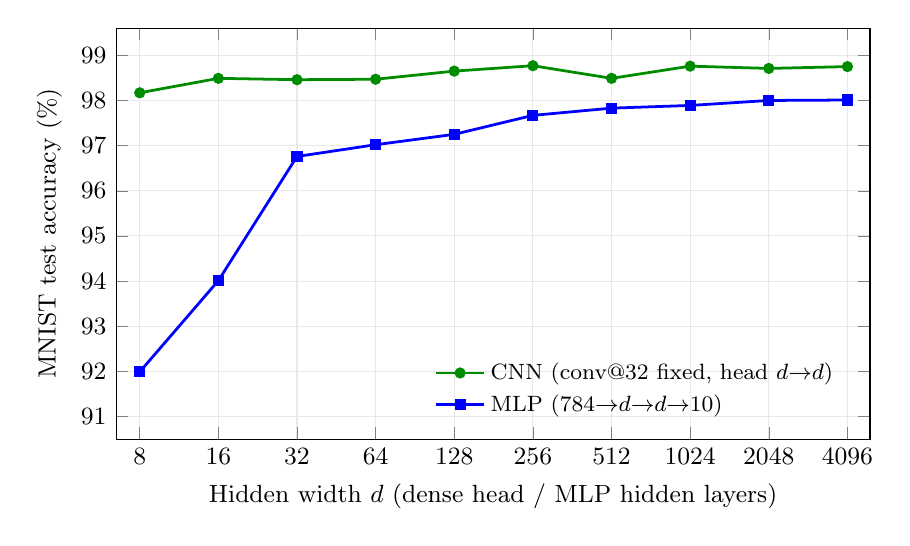
\begin{tikzpicture}
\begin{axis}[
    width=0.92\linewidth, height=6.8cm,
    xlabel={Hidden width $d$ (dense head / MLP hidden layers)},
    ylabel={MNIST test accuracy (\%)},
    xmode=log, log basis x=2,
    xmin=6.5, xmax=5000, ymin=90.5, ymax=99.6,
    xtick={8,16,32,64,128,256,512,1024,2048,4096},
    xticklabels={8,16,32,64,128,256,512,1024,2048,4096},
    ytick={91,92,93,94,95,96,97,98,99},
    legend pos=south east, legend cell align={left},
    legend style={font=\footnotesize, draw=none, fill=none},
    grid=major, grid style={gray!18},
    tick label style={font=\small},
    label style={font=\small},
    every axis plot/.append style={line width=1pt, mark size=1.5pt},
]
\addplot[green!55!black, mark=*, mark options={fill=green!55!black}] coordinates {
(8,98.17) (16,98.49) (32,98.46) (64,98.47) (128,98.65) (256,98.77) (512,98.49) (1024,98.76) (2048,98.71) (4096,98.75)
};
\addlegendentry{CNN (conv@32 fixed, head $d{\to}d$)}
\addplot[blue, mark=square*, mark options={fill=blue}] coordinates {
(8,91.99) (16,94.01) (32,96.76) (64,97.02) (128,97.25) (256,97.67) (512,97.83) (1024,97.89) (2048,98.00) (4096,98.01)
};
\addlegendentry{MLP ($784{\to}d{\to}d{\to}10$)}
\end{axis}
\end{tikzpicture}
\end{center}

\noindent Classifier-head width sweep for the verified CNN (convolutional
backbone held at 32 channels), overlaid on the MLP width sweep of
Chapter~\ref{chap:mlp} (\texttt{runs/cnn\_grid\_rep\{1..5\}.tsv} and
\texttt{runs/mlp\_grid\_results\_xla.tsv}). Each CNN point is the median of
five runs, because two of the widths are bimodal: $d=512$ and $d=4096$ each
produced one run about 2 and 5 points below their other four, while the
other eight widths repeat to within 0.4. The MLP points are single runs,
which is enough because that graph is dense-only and reproduces exactly.
The whole CNN curve sits about a point above the MLP's, and it is flat
across the entire range: an 8-wide head already reaches 98.2\% at 60K
parameters, beating the widest 4096-wide MLP. So the 3.2M-parameter
$6272{\to}512$ layer is not buying accuracy, because shrinking the head
to $\ldots{\to}8{\to}8{\to}10$ keeps essentially all of it. The head is fat
because the flatten hands it a 6272-vector and nobody trimmed it, not
because the task needs the width. There is no knee to find here, and the
convolutional backbone has already done the work the head is being paid
for. (On this GPU the wall-clock is convolution-bound, so
the shrink is a parameter win rather than a speed win, which is exactly why
the post-2015 fix was \texttt{globalAvgPool}, replacing the flatten rather
than narrowing it.)

\section{MLIR: Convolution}

\noindent\textbf{What is already proven.} \texttt{cnnForward} is
the conv\,$\to$\,relu\,$\to$\,conv\,$\to$\,relu\,$\to$\,maxPool\,$\to$\,flatten\,$\to$\,dense
network, and \texttt{cnn\_has\_vjp\_at} proves its reverse-mode derivative
by chaining the per-layer VJPs: the dense backward
(\S~\ref{thm:dense_has_vjp}, reused from Chapter~\ref{chap:mlp}), the
max-pool backward (\texttt{maxPool2\_has\_vjp3},
\S~\ref{ax:maxPool2_has_vjp3}), and the convolution backward
(\texttt{conv2d\_has\_vjp3}, \S~\ref{ax:conv2d_has_vjp3}), all through the
IR-level chain rule \texttt{vjp\_comp\_at}. The convolution's reverse-mode
derivative is the chapter's headline result: the input VJP of a
\texttt{conv2d} is \emph{another} \texttt{conv2d}, against the kernel with
its in- and out-channels swapped and both spatial axes reversed. The
parameter gradients are pinned by \texttt{conv2d\_weight\_grad\_has\_vjp}
(the transpose trick) and the dense grads from Chapter~\ref{chap:mlp}, and
the loss gradient by \texttt{softmaxCE\_grad} (\S~\ref{ax:softmaxCE_grad}).
So \emph{what} the convolution's gradient is, is not in question.

\medskip\noindent\textbf{The gap and how we close it.} The emitted
backward convolution is given a denotation $[\![\cdot]\!]$ valued in the
proofs' own tensor type,
\[
  [\![\texttt{convBackDenote}\,W]\!]
  = \texttt{conv2d}\,(\texttt{reverseSwap}\,W),
  \qquad
  (\texttt{reverseSwap}\,W)_{c_i\,c_o\,k_h\,k_w} = W_{c_o\,c_i\,\bar k_h\,\bar k_w},
\]
where $\bar k = K - 1 - k$ is the spatial flip, and the bridge theorem
\[
  \texttt{conv\_back\_bridge\_1to2}:\quad
  [\![\texttt{convBackDenote}\,W]\!](dy)
  = (\texttt{conv2d\_has\_vjp3}\,W\,b).\mathrm{backward}(x, dy)
\]
says the denotation of that graph is the proven conv input-VJP, the
reversed-kernel identity that \texttt{cnn\_has\_vjp\_at} only \emph{asserts}.
It is discharged here by expansion at the concrete shape (and again at the
$2{\to}2$ shape, by \texttt{conv\_back\_bridge\_2to2}). The printer walks the
graph and emits one \texttt{stablehlo} op per node: \texttt{transpose}
for the channel swap, \texttt{reverse} for the spatial flip,
\texttt{convolution} for the contraction:

Here is exactly what the printer emits for the first conv's backward
($1{\to}2$ channels, $3\times3$ kernel, at $4\times4$):

\begin{verbatim}
func.func @conv_back(%dy: tensor<1x2x4x4xf32>,
    %W: tensor<2x1x3x3xf32>) -> tensor<1x1x4x4xf32> {
  %Wt = stablehlo.transpose %W, dims = [1, 0, 2, 3]
          : (tensor<2x1x3x3xf32>) -> tensor<1x2x3x3xf32>
  %Wr = stablehlo.reverse %Wt, dims = [2, 3] : tensor<1x2x3x3xf32>
  %dx = stablehlo.convolution(%dy, %Wr)
      dim_numbers = [b, f, 0, 1]x[o, i, 0, 1]->[b, f, 0, 1],
      window = {stride = [1, 1], pad = [[1, 1], [1, 1]],
                lhs_dilate = [1, 1], rhs_dilate = [1, 1]}
      : (tensor<1x2x4x4xf32>, tensor<1x2x3x3xf32>)
          -> tensor<1x1x4x4xf32>
  return %dx : tensor<1x1x4x4xf32>
}
\end{verbatim}

\noindent Read it against the graph: \texttt{\%Wt} is the
\texttt{transpose dims [1,0,2,3]} that swaps the kernel's out- and
in-channel axes, and \texttt{\%Wr} is the \texttt{reverse dims [2,3]} that
flips both spatial axes ($\bar k_h,\bar k_w$). Together they build
\texttt{reverseSwap}\,$W$. The \texttt{convolution} then convolves the
incoming cotangent \texttt{\%dy} against that kernel, exactly
$\texttt{conv2d}\,(\texttt{reverseSwap}\,W)$, the
$1\,\text{channel} \leftarrow 2\,\text{channels}$ adjoint of the forward
conv. The bridge theorem is precisely the claim that this text computes
\texttt{conv2d\_has\_vjp3}'s backward. The max-pool, flatten, dense, and
relu nodes of the full backward are bridged the same way, and the max-pool
tile-compare-select by \texttt{maxpool\_back\_bridge}, the dense
\texttt{dot\_general}s exactly as in Chapter~\ref{chap:mlp}, so the
whole CNN backward is covered, op by op.

\medskip\noindent\textbf{Caveats.}
\begin{itemize}
  \item \textbf{The convolution bridge is unconditional.} A convolution
    is linear, so it holds at every input.
  \item \textbf{ReLU is a smooth-point bridge} (no pre-activation exactly
    zero), failing only on that measure-zero set.
  \item \textbf{Max-pool needs a unique argmax.} The bridge holds only
    where every $2\times2$ window has a strict argmax. The tie set is the
    codegen trust boundary for pooling.
  \item \textbf{Representative scale.} $1{\to}2$ channels at $4\times4$
    (production: $1{\to}32$ at $28\times28$).
\end{itemize}

\chapter{CIFAR with BatchNorm}
\label{chap:bn}

This chapter is the bridge between the MNIST chapters and the
deep-network chapters that follow. Chapter~\ref{chap:cnn} did MNIST
with a two-convolution net and a 2$\times$512 dense head.
Chapter~\ref{chap:residual} (ResNet-34) goes thirty-four layers deep.
The network here sits exactly in between. It keeps MNIST's
\emph{same} 2$\times$512 head and the same conv/ReLU/max-pool
machinery, but stacks the convolutions four stages deep (eight in all)
on a harder dataset (CIFAR-10). That is the first point in the book
where depth is enough to make two things bite: \textbf{BatchNorm starts
to earn its keep, and the choice of optimizer starts to matter}. The
depth itself is what ResNet then scales to thirty-four layers. So
the chapter has two jobs: prove the one new operator (BatchNorm), and
use the deeper net to measure what actually governs training
(\S\ref{sec:bn_cifar_example}).

Proving BN is also what makes this \textbf{structurally the hardest
chapter in the book}. BN's
inverse-stddev term \(1/\sqrt{\sigma^2 + \varepsilon}\) has a
gradient that blows up as \(\sigma^2 \to 0\). Proving the
backward pass exists and is bounded requires
\texttt{ContinuousLinearMap}-based real-analysis machinery from
Mathlib that none of the previous chapters needed.
\textbf{If you're new to formal math, skim the proofs and trust
them}. The takeaways are concrete:

\begin{itemize}
\item BN's gradient has a closed-form 3-term formula
  (Theorem~\ref{thm:bnNormalize_has_vjp}).
\item The formula needs \(\varepsilon > 0\) to stay bounded
  (Theorem~\ref{ax:bnIstdBroadcast_diff}).
\item BN's payoff is \emph{speed} and \emph{stability}: a deeper
  network reaches the same accuracy in far fewer epochs with it than
  without, and under a strong optimizer the un-normalized net does not
  reliably finish training at all. The example in
  \S\ref{sec:bn_cifar_example} measures both directly.
\end{itemize}

The proofs themselves use Mathlib's \texttt{HasFDerivAt.sqrt},
\texttt{(hasDerivAt\_inv).comp\_hasFDerivAt}, and a centering CLM
chained through the chain rule from Ch~\ref{chap:tensor}. They're
correct (the Lean kernel checks them) and they're available in
\texttt{Proofs/BatchNorm.lean} for the curious. You do not need to
understand them line-by-line to use BN as a layer or to follow the
rest of the book. \textbf{Ch~\ref{chap:residual} (ResNet-34) is
the easiest chapter in the book and follows immediately. This
is a localized difficulty spike, not the new normal.}

\prosesection{What BN actually is}

BatchNorm (Ioffe \& Szegedy, 2015) takes a batch of activations,
\(x\), and does three things in sequence. Each is one line of code.
Together they are the layer.

\begin{enumerate}
\item \textbf{Center.} Compute the batch mean
  \(\mu = \frac{1}{n} \sum_k x_k\) and subtract it from every sample:
  \(x - \mu\). Output has mean zero.
\item \textbf{Normalize.} Compute the batch variance \(\sigma^2\),
  add a small \(\varepsilon\) for numerical safety, and divide:
  \(\hat{x} = (x - \mu)/\sqrt{\sigma^2 + \varepsilon}\). Output has
  unit variance.
\item \textbf{Affine.} Scale and shift with learnable per-channel
  parameters \(\gamma\) and \(\beta\): \(\mathrm{bn}(x) = \gamma \hat{x} + \beta\).
\end{enumerate}

The chapter's first six theorems are the Jacobian of each step
and the VJPs that fall out of them. Theorem
\ref{thm:bn_has_vjp} closes the loop by composing them. The
forward is three steps, so the chain rule from
Chapter~\ref{chap:tensor} gives us three Jacobians to multiply,
and the ``BN three-term backward'' is exactly that
product written out.

\section{Run it first}
\label{sec:bn_runit}

Before any of the math, train the thing. Four commands and about
thirteen minutes of GPU time:

\begin{verbatim}
lake exe cache get                            # Mathlib oleans, ~30 s
./download_cifar.sh                           # ~170 MB
lake build cifar8w-bn-ablation
./.lake/build/bin/cifar8w-bn-ablation data
\end{verbatim}

That one binary runs the same network three times, once per optimizer.
Here is the second of the three, on one RTX 4060 Ti (CUDA 12.9), from
\texttt{runs/2026-08-12-cifar8w-6arm-xla-cuda/cifar8w-bn-p1.log}. XLA's
startup banner is removed, the per-step loss lines are dropped, and
epochs 8 through 34 are elided:

\begin{verbatim}
[pjrt_ffi] XLA backend: PJRT 0.112, 1 device(s)
[pjrt_ffi] compiled verified_mlir/cifar8w_bn_mom_train_step.mlir
             (@cifar8w_bn_mom_train_step, 117 outputs, 1 replica) in 1215 ms
[pjrt_ffi] compiled verified_mlir/cifar8w_bn_fwd.mlir
             (@cifar8w_bn_fwd, 1 outputs, 1 replica) in 261 ms
════════ cifar8w-BN (wide head) — Nesterov momentum (μ.9, lr 0.02) ════════
Deeper CIFAR-10 CNN + per-channel BatchNorm, MNIST-style wide head
  (8× conv→BN→relu → 128→512→512→10) via the VERIFIED renderer → XLA/PJRT → GPU
  xla/pjrt verified_mlir/cifar8w_bn_mom_train_step.mlir
  xla/pjrt verified_mlir/cifar8w_bn_fwd.mlir
  train 50000, test 10000; bs 128, CIFAR-CNN8-wide-BN mom
    (cosine+warmup 3ep, baseLR 0.020000), He init
Epoch 1/40: loss=1.958118 lr=0.006667
  epoch 1: test_acc = 4209/10000 = 42.090000%  top5 = 8952/10000 = 89.520000%
Epoch 2/40: loss=1.418591 lr=0.013333
  epoch 2: test_acc = 5474/10000 = 54.740000%  top5 = 9449/10000 = 94.490000%
Epoch 3/40: loss=1.167188 lr=0.020000
  epoch 3: test_acc = 6022/10000 = 60.220000%  top5 = 9523/10000 = 95.230000%
Epoch 4/40: loss=0.992680 lr=0.019964
  epoch 4: test_acc = 6499/10000 = 64.990000%  top5 = 9694/10000 = 96.940000%
Epoch 5/40: loss=0.882675 lr=0.019856
  epoch 5: test_acc = 6876/10000 = 68.760000%  top5 = 9726/10000 = 97.260000%
Epoch 6/40: loss=0.811264 lr=0.019677
  epoch 6: test_acc = 6997/10000 = 69.970000%  top5 = 9771/10000 = 97.710000%
Epoch 7/40: loss=0.756665 lr=0.019429
  epoch 7: test_acc = 7208/10000 = 72.080000%  top5 = 9784/10000 = 97.840000%
Epoch 35/40: loss=0.258739 lr=0.000888
  epoch 35: test_acc = 7759/10000 = 77.590000%  top5 = 9836/10000 = 98.360000%
Epoch 36/40: loss=0.251148 lr=0.000571
  epoch 36: test_acc = 7738/10000 = 77.380000%  top5 = 9832/10000 = 98.320000%
Epoch 37/40: loss=0.247924 lr=0.000323
  epoch 37: test_acc = 7750/10000 = 77.500000%  top5 = 9840/10000 = 98.400000%
Epoch 38/40: loss=0.246187 lr=0.000144
  epoch 38: test_acc = 7753/10000 = 77.530000%  top5 = 9839/10000 = 98.390000%
Epoch 39/40: loss=0.241790 lr=0.000036
  epoch 39: test_acc = 7751/10000 = 77.510000%  top5 = 9841/10000 = 98.410000%
Epoch 40/40: loss=0.243040 lr=0.000000
  epoch 40: test_acc = 7748/10000 = 77.480000%  top5 = 9840/10000 = 98.400000%
done (trained CIFAR-CNN8-wide-BN mom + cosine/warmup via packed threading).
\end{verbatim}

Forty epochs at about six seconds each, and 77.48\% on the full
10,000-image CIFAR-10 test set, 98.40\% inside the top five. CIFAR-10
is a much harder problem than MNIST, so this is the first chapter where
the headline accuracy drops out of the nineties.

BatchNorm's backward is the first in this book you can't read off by
inspection. That run did not execute a
reimplementation of the network this chapter describes. It executed
\texttt{verified\_mlir/cifar8w\_bn\_mom\_train\_step.mlir}, which is the
text \texttt{Proofs.StableHLO} emits for this net, and
\texttt{Proofs/Cifar8Close.lean} proves that each of its parameter
updates denotes the certified softmax cross-entropy loss-descent step
derived from the Mathlib \(\fderiv\) math. Every BatchNorm in it computes
the three-term backward this chapter proves.

The two compile lines carry the whole in-process story. The train step
and the eval forward are handed to XLA once, as text, and compiled in
about 1.5 seconds together, after which all forty epochs run without
leaving the process.

\S\ref{sec:bn_cifar_example} runs this same binary and its no-BN peer
across all three optimizers, which is where the chapter's measurements
come from, and \texttt{lake run cifar} is those two binaries.

\prosesection{The centering term has an indirect path}

When you
jiggle a single input \(x_i\), you do not only jiggle \(x_i\). You
also jiggle the batch mean \(\mu\), and \(\mu\) appears in every
sample's centered value \(x_k - \mu\). So jiggling \(x_i\) by
\(\varepsilon\) shifts every centered value by \(-\varepsilon/n\)
\emph{plus} the direct \(\varepsilon\) on the \(i\)th sample.

\[
\frac{\partial (x_j - \mu)}{\partial x_i} \;=\; \delta_{ij} - \frac{1}{n}.
\]

The \(\delta_{ij}\) is the direct effect. The \(-1/n\) is the
indirect effect through \(\mu\). Theorem \ref{ax:pdiv_bnCentered}
states this formally. Forgetting the \(-1/n\) is the most common
hand-derivation mistake on BN, and is exactly what the formal
proof prevents.

\prosesection{The inverse-stddev term}

The normalize step divides by \(\sqrt{\sigma^2 + \varepsilon}\),
where \(\sigma^2 = \frac{1}{n} \sum_k (x_k - \mu)^2\) is itself a
function of every input. Jiggle \(x_i\) by \(\varepsilon\) and
\(\sigma^2\) changes, which means the divisor changes, which means
\emph{every} output \(\hat{x}_j\) changes, not just \(\hat{x}_i\).

Working through the chain rule (\(x \mapsto x^2 \mapsto \text{mean}
\mapsto \sqrt{\cdot + \varepsilon} \mapsto 1/\cdot\)) gives

\[
\frac{\partial}{\partial x_i} \frac{1}{\sqrt{\sigma^2 + \varepsilon}}
\;=\; -\frac{1}{(\sigma^2 + \varepsilon)^{3/2}} \cdot \frac{x_i - \mu}{n}
\;=\; -\,\mathrm{istd}^3 \cdot \frac{x_i - \mu}{n}.
\]

That \(\mathrm{istd}^3\) is what makes the BN backward expensive:
the gradient of one sample depends on \emph{every} sample's
centered value, scaled by the cube of the inverse standard
deviation. Theorem \ref{ax:pdiv_bnIstdBroadcast} states this.

Notice what happens to the formula as \(\sigma^2 \to 0\):
\(\mathrm{istd} \to 1/\sqrt{\varepsilon}\), bounded. Without \(\varepsilon\)
the gradient diverges. Theorem \ref{ax:bnIstdBroadcast_diff} is
the formal statement that \(\varepsilon > 0\) is sufficient to
make this term differentiable. This is the \emph{one place in
the book} where the math actually requires real-analysis machinery
beyond chain-sum-product. Everything else in the framework reduces
to those three rules.

\prosesection{The three-term backward}

Compose the three forward steps and apply the product rule on
\(\hat{x} = (x - \mu) \cdot \mathrm{istd}\). The cross-terms collapse
(the centered sum \(\sum_k (x_k - \mu) = 0\) is what saves us) and
what falls out is a one-line backward:

\[
dx \;=\; \frac{\mathrm{istd} \cdot \gamma}{n}\, \Bigl(\, n\,dy
  \;-\; \textstyle\sum_k dy_k
  \;-\; \hat{x} \cdot \textstyle\sum_k (dy_k \,\hat{x}_k)\, \Bigr).
\]

Three terms inside the parentheses, one per forward step's
indirect effect:

\begin{itemize}
\item \(n\,dy\): the direct effect, every sample's upstream gradient.
\item \(-\sum_k dy_k\): the centering correction, subtracts the
  total upstream gradient because shifting the mean shifts every
  sample.
\item \(-\hat{x} \cdot \sum_k (dy_k\,\hat{x}_k)\): the normalization
  correction, subtracts the projection of the upstream gradient onto
  \(\hat{x}\), because rescaling by the inverse stddev couples
  every sample's gradient through the shared divisor.
\end{itemize}

Theorem \ref{thm:bnNormalize_has_vjp} formalizes this. Every
production BN implementation (PyTorch, JAX, TensorFlow, custom
CUDA kernels) computes this exact expression. The formula has been
known since 2015. The \emph{value} of the formal proof is that the
Lean kernel mechanically verifies we are computing the right thing
at every training step.

\prosesection{The affine step is dense-with-broadcasting}

The third step, \(\gamma \hat{x} + \beta\), is structurally a
dense layer applied per-channel. Its Jacobian
\(\partial(\gamma v + \beta)/\partial v_i = \gamma \delta_{ij}\) is
exactly the dense-Jacobian computation from
Chapter~\ref{chap:mlp}, just lifted to a tensor shape and
broadcast across spatial dimensions. Theorem
\ref{ax:pdiv_bnAffine} and Theorem \ref{thm:bnAffine_has_vjp}
are essentially corollaries of the dense theorems. The new content
here is zero.

\prosesection{Putting it together}

Theorem \ref{thm:bn_has_vjp} is the composition:
\(\mathrm{bn} = \mathrm{affine} \circ \mathrm{normalize}\), with VJPs
chained via the same \(\mathrm{vjp\_comp}\) rule from
Chapter~\ref{chap:tensor}. The 3-term backward is the
centerpiece, affine is a corollary, and composition is a one-line
proof. The structural story of the chapter is: one new
Mathlib-level analytic dependency (sqrt and recip
differentiability), one formula, and the rest is the same
chain rule we already had.

\section{The theorems}

\begin{theorem}[BN affine step Jacobian]
  \label{ax:pdiv_bnAffine}
  \lean{Proofs.pdiv_bnAffine}
  \leanok
  \uses{ax:pdiv, ax:pdiv_add, ax:pdiv_mul, ax:pdiv_const, ax:pdiv_id}
  For \(\mathrm{bnAffine}(\gamma, \beta)\, v = \lambda i.\;
  \gamma v_i + \beta\):
  \Prove{} \(\pdiv\bigl(\mathrm{bnAffine}(\gamma, \beta)\bigr)\, v\, i\, j
    = \gamma\, \delta_{ij}\).
\end{theorem}

\begin{proof}
\leanok
\begin{enumerate}
  \item \(\pdiv\bigl(\mathrm{bnAffine}(\gamma, \beta)\bigr)\, v\, i\, j
          = \pdiv(y \mapsto \gamma \cdot y)\, v\, i\, j\).
    \pf{Split \(\gamma v_i + \beta\) as
    \((\gamma \cdot v) + (\text{const } \beta)\): sum rule
    (Theorem~\ref{ax:pdiv_add}) and constant rule
    (Theorem~\ref{ax:pdiv_const}).}
  \item \(\pdiv(y \mapsto \gamma \cdot y)\, v\, i\, j
          = \gamma\, \delta_{ij}\).
    \pf{Factor as \((\text{const } \gamma) \cdot (\text{identity})\):
    product rule (Theorem~\ref{ax:pdiv_mul}); the constant factor's
    Jacobian vanishes (Theorem~\ref{ax:pdiv_const}) and the identity
    Jacobian is \(\delta_{ij}\) (Theorem~\ref{ax:pdiv_id}).}
  \item \Qed{}
    \pf{Chain 1 and 2.}
\end{enumerate}
\end{proof}

\begin{theorem}[BN centering Jacobian]
  \label{ax:pdiv_bnCentered}
  \lean{Proofs.pdiv_bnCentered}
  \leanok
  \uses{ax:pdiv, ax:pdiv_add, ax:pdiv_mul, ax:pdiv_const, ax:pdiv_id, thm:pdiv_finset_sum, ax:pdiv_reindex}
  For \(\mathrm{bnCentered}\, x = \lambda j.\; x_j - \mu(x)\), where
  \(\mu(x) = \frac{1}{n}\sum_s x_s\):
  \Prove{} \(\pdiv(\mathrm{bnCentered})\, x\, i\, j
    = \delta_{ij} - 1/n\).
\end{theorem}

\begin{proof}
\leanok
\begin{enumerate}
  \item \(\pdiv(\mathrm{bnCentered})\, x\, i\, j
          = \delta_{ij}
            + \pdiv\bigl(y \mapsto -\tfrac{1}{n}\textstyle\sum_s y_s\bigr)\, x\, i\, j\).
    \pf{\(\mathrm{bnCentered} = \mathrm{id} + \bigl(y \mapsto
    -(\sum_s y_s)/n\bigr)\): sum rule (Theorem~\ref{ax:pdiv_add}),
    identity Jacobian (Theorem~\ref{ax:pdiv_id}).}
  \item \(\pdiv\bigl(y \mapsto -\tfrac{1}{n}\textstyle\sum_s y_s\bigr)\, x\, i\, j
          = -\tfrac{1}{n} \cdot
            \pdiv\bigl(y \mapsto \textstyle\sum_s y_s\bigr)\, x\, i\, j\).
    \pf{Factor as \((\text{const } -\tfrac{1}{n}) \cdot (\text{sum})\):
    product rule (Theorem~\ref{ax:pdiv_mul}); the constant factor's
    Jacobian vanishes (Theorem~\ref{ax:pdiv_const}).}
  \item \(\pdiv\bigl(y \mapsto \textstyle\sum_s y_s\bigr)\, x\, i\, j
          = \sum_s \delta_{is} = 1\).
    \pf{Finite-sum rule (Theorem~\ref{thm:pdiv_finset_sum}) over the
    coordinate projections; each projection is a reindex with
    Jacobian \(\delta_{is}\) (Theorem~\ref{ax:pdiv_reindex});
    the Kronecker sum collapses (\texttt{Finset.sum\_ite\_eq}).}
  \item \Qed{}
    \pf{Chain 1--3: \(\delta_{ij} + (-\tfrac{1}{n}) \cdot 1
      = \delta_{ij} - 1/n\).}
\end{enumerate}
\end{proof}

\begin{theorem}[BN inverse-stddev broadcast smoothness]
  \label{ax:bnIstdBroadcast_diff}
  \lean{Proofs.bnIstdBroadcast_diff}
  \leanok
  \Assume{}
  \begin{enumerate}
    \item \(\varepsilon > 0\) \hfill[\texttt{h\(\varepsilon\)}]
  \end{enumerate}
  \Prove{} \(\bnIstdBroadcast = x \mapsto 1/\sqrt{\sigma^2(x) + \varepsilon}\)
  is \(\Differentiable\). This is the sqrt/recip smoothness that the
  product rule needs inside the normalize Jacobian.
\end{theorem}

\begin{proof}
\leanok
\begin{enumerate}
  \item \(\sigma^2(x) + \varepsilon > 0\) for every \(x\), in
    particular \(\neq 0\).
    \pf{\(\sigma^2(x) \ge 0\) (a sum of squares over \(n\));
    assumption 1 pushes it strictly positive.}
  \item \(x \mapsto \sigma^2(x) + \varepsilon\) is differentiable.
    \pf{Polynomial in the coordinates of \(x\) (\texttt{fun\_prop}).}
  \item \(x \mapsto \sqrt{\sigma^2(x) + \varepsilon}\) is
    differentiable, and nowhere zero.
    \pf{\texttt{Differentiable.sqrt} applies away from \(0\), which 1
    grants; \(\sqrt{\cdot}\) of a positive is positive.}
  \item \Qed{}
    \pf{\(\mathrm{istd} = (\sqrt{\sigma^2 + \varepsilon})^{-1}\);
    \texttt{Differentiable.inv} with the nonvanishing denominator
    from 3.}
\end{enumerate}
\end{proof}

\begin{theorem}[BN inverse-stddev broadcast Jacobian]
  \label{ax:pdiv_bnIstdBroadcast}
  \lean{Proofs.pdiv_bnIstdBroadcast}
  \leanok
  \uses{ax:pdiv, ax:bnIstdBroadcast_diff}
  \Assume{}
  \begin{enumerate}
    \item \(\varepsilon > 0\) \hfill[\texttt{h\(\varepsilon\)}]
  \end{enumerate}
  \Prove{} writing \(s := \mathrm{istd}(x, \varepsilon)
    = 1/\sqrt{\sigma^2(x) + \varepsilon}\):
  \[
    \pdiv(\bnIstdBroadcast)\, x\, i\, j
      = -s^3 \cdot (x_i - \mu)/n.
  \]
\end{theorem}

\begin{proof}
\leanok
\emph{Sketch: the one genuinely analytic Jacobian of the chapter ---
a Fréchet-derivative chain through variance, \(\sqrt{\cdot}\), and
\(({\cdot})^{-1}\), closed by the \(\sum_k (x_k - \mu) = 0\)
identity.}
\begin{enumerate}
  \item \(\sigma^2(x) + \varepsilon > 0\), so
    \(\sqrt{\sigma^2(x) + \varepsilon} > 0\).
    \pf{Sum of squares \(\ge 0\) plus assumption 1.}
  \item \(\pdiv(\bnIstdBroadcast)\, x\, i\, j
          = \fderiv_{\R}\,\bigl(x' \mapsto \mathrm{istd}(x', \varepsilon)\bigr)\, x\, (\basisVec_i)\)
    --- the output is constant in \(j\), so \(\pdiv\) reduces to the
    scalar derivative.
    \pf{Definition~\ref{ax:pdiv} and \texttt{fderiv\_apply},
    legitimate by Theorem~\ref{ax:bnIstdBroadcast_diff}.}
  \item Derivative chain. Let \(C_k := \mathrm{proj}_k -
    \tfrac{1}{n}\sum_{i'} \mathrm{proj}_{i'}\) be the centering CLM
    (so \(C_k\, y = y_k - \mu(y)\)). Then
    \(\sigma^2 = \tfrac{1}{n}\sum_k C_k^2\) has Fréchet derivative
    \(\tfrac{1}{n}\sum_k 2\, C_k(x) \cdot C_k\), and composing
    through \(\sqrt{\cdot}\) (\texttt{HasFDerivAt.sqrt}, licensed by
    1) and \(({\cdot})^{-1}\) (\texttt{hasDerivAt\_inv}) gives
    \(\partial\, \mathrm{istd} / \partial \sigma^2
      = -\tfrac{1}{2}\, s^3\).
    \pf{Product rule per square, summed; the two Mathlib
    compositions.}
  \item Evaluate at \(\basisVec_i\):
    \(\partial \sigma^2 / \partial x_i = \tfrac{2}{n}(x_i - \mu)\).
    \pf{\(C_k(\basisVec_i) = \delta_{ki} - \tfrac{1}{n}\), so the sum
    in 3 is \(\tfrac{2}{n} \sum_k (x_k - \mu)(\delta_{ki} - \tfrac{1}{n})\),
    which collapses to \(\tfrac{2}{n}(x_i - \mu)\) because
    \(\sum_k (x_k - \mu) = 0\).}
  \item \Qed{}
    \pf{Chain 3 and 4:
    \(-\tfrac{1}{2}\, s^3 \cdot \tfrac{2}{n}(x_i - \mu)
      = -s^3 (x_i - \mu)/n\); with 2 this is the goal.}
\end{enumerate}
\end{proof}

\begin{theorem}[BN normalize 3-term VJP]
  \label{thm:bnNormalize_has_vjp}
  \lean{Proofs.bnNormalize_has_vjp}
  \leanok
  \uses{ax:pdiv_bnCentered, ax:pdiv_bnIstdBroadcast, ax:bnIstdBroadcast_diff, ax:pdiv_mul, def:hasvjp}
  \Assume{}
  \begin{enumerate}
    \item \(\varepsilon > 0\) \hfill[\texttt{h\(\varepsilon\)}]
  \end{enumerate}
  \Prove{} \(\HasVJP\, (\mathrm{bnNormalize})\), with the consolidated
  three-term backward (writing \(s := \mathrm{istd}\),
  \(\hat{x} := \mathrm{bnXhat}\)):
  \[
    B(x, d\hat{x})_i = \tfrac{1}{n}\, s \Bigl(
      n\, d\hat{x}_i - \sum_j d\hat{x}_j
      - \hat{x}_i \sum_j \hat{x}_j\, d\hat{x}_j \Bigr).
  \]
\end{theorem}

\begin{proof}
\leanok
\emph{Sketch: product rule on \(\hat{x} = (x - \mu) \cdot s\) merges
the two elementary Jacobians into one formula; contracting with
\(d\hat{x}\) splits it into the three terms.}
\begin{enumerate}
  \item Consolidated Jacobian:
    \(\pdiv(\mathrm{bnNormalize})\, x\, i\, j
      = \tfrac{s}{n}\bigl(n\, \delta_{ij} - 1 - \hat{x}_i \hat{x}_j\bigr)\).
    \pf{Factor \(\hat{x}\) as the elementwise product
    \(\mathrm{bnCentered} \cdot \bnIstdBroadcast\)
    (\texttt{bnXhat\_eq\_product}); product rule
    (Theorem~\ref{ax:pdiv_mul}) --- differentiable because
    \(\mathrm{bnCentered}\) is affine and \(\bnIstdBroadcast\) is
    smooth (Theorem~\ref{ax:bnIstdBroadcast_diff}, assumption 1);
    substitute the centering Jacobian
    (Theorem~\ref{ax:pdiv_bnCentered}) and the istd Jacobian
    (Theorem~\ref{ax:pdiv_bnIstdBroadcast}); the
    \(\hat{x} = (x - \mu) \cdot s\) identity plus
    \texttt{field\_simp}/\texttt{ring} collapse the algebra
    (\(n \neq 0\) since \(\mathrm{Fin}\, n\) is inhabited by \(i\)).
    This step is the Lean lemma \texttt{pdiv\_bnNormalize}.}
  \item \Suffices{} for all \(x\), \(d\hat{x}\), \(i\):
    \(B(x, d\hat{x})_i = \sum_j \pdiv(\mathrm{bnNormalize})\, x\, i\, j
      \cdot d\hat{x}_j\).
    \pf{Definition~\ref{def:hasvjp}, with \(B\) as the candidate
    backward function.}
  \item \Qed{}
    \pf{Substitute 1 into 2 and split the sum into its three pieces:
    the \(\delta\)-term collapses to \(n\, d\hat{x}_i\)
    (\texttt{Finset.sum\_ite\_eq}), the \(-1\) term gives
    \(-\sum_j d\hat{x}_j\), and factoring \(\hat{x}_i\) out of the
    third gives \(-\hat{x}_i \sum_j \hat{x}_j d\hat{x}_j\); scale by
    \(s/n\) and this is \(B\).}
\end{enumerate}
\end{proof}

\begin{theorem}[BN affine VJP]
  \label{thm:bnAffine_has_vjp}
  \lean{Proofs.bnAffine_has_vjp}
  \leanok
  \uses{ax:pdiv_bnAffine, def:hasvjp}
  \(\HasVJP\, \bigl(\mathrm{bnAffine}(\gamma, \beta)\bigr)\): each
  input feeds one output scaled by \(\gamma\), so the gradient comes
  back scaled by \(\gamma\).
\end{theorem}

\begin{proof}
\leanok
\begin{enumerate}
  \item Define \(B(v, dy)_i := \gamma \cdot dy_i\).
  \item \Suffices{} for all \(v\), \(dy\), \(i\):
    \(B(v, dy)_i = \sum_j
      \pdiv\bigl(\mathrm{bnAffine}(\gamma, \beta)\bigr)\, v\, i\, j \cdot dy_j\).
    \pf{Definition~\ref{def:hasvjp}, with \(B\) as the candidate
    backward function.}
  \item \Qed{}
    \pf{By the affine Jacobian (Theorem~\ref{ax:pdiv_bnAffine}) the
    sum is \(\sum_j \gamma\, \delta_{ij}\, dy_j = \gamma\, dy_i\).}
\end{enumerate}
\end{proof}

\begin{theorem}[Full BN VJP]
  \label{thm:bn_has_vjp}
  \lean{Proofs.bn_has_vjp}
  \leanok
  \uses{thm:bnNormalize_has_vjp, thm:bnAffine_has_vjp, thm:vjp_comp, ax:bnIstdBroadcast_diff}
  \Assume{}
  \begin{enumerate}
    \item \(\varepsilon > 0\) \hfill[\texttt{h\(\varepsilon\)}]
  \end{enumerate}
  \Prove{} \(\HasVJP\, \bigl(\mathrm{bnForward}(\varepsilon, \gamma,
  \beta)\bigr)\).
\end{theorem}

\begin{proof}
\leanok
\begin{enumerate}
  \item \(\mathrm{bnForward} = \mathrm{bnAffine} \circ
    \mathrm{bnNormalize}\).
    \pf{Definitional (\texttt{bnForward\_eq\_compose}).}
  \item \(\mathrm{bnNormalize}\) is differentiable everywhere.
    \pf{It is the elementwise product of \(\mathrm{bnCentered}\)
    (affine, hence smooth) and \(\bnIstdBroadcast\) (smooth by
    Theorem~\ref{ax:bnIstdBroadcast_diff}, assumption 1).}
  \item \(\mathrm{bnAffine}\) is differentiable everywhere.
    \pf{Affine (\texttt{fun\_prop}).}
  \item \Qed{}
    \pf{VJP chain rule (Theorem~\ref{thm:vjp_comp}) with 2, 3 and the
    two halves (Theorems~\ref{thm:bnNormalize_has_vjp},
    \ref{thm:bnAffine_has_vjp}). The composed backward is exactly the
    two-step MLIR backward: \(d\hat{x} = \gamma \cdot dy\), then the
    three-term formula.}
\end{enumerate}
\end{proof}

\section{Example: training dynamics on CIFAR}
\label{sec:bn_cifar_example}

Chapter~\ref{chap:cnn} did MNIST with two convolutions and a
2$\times$512 dense head. This chapter keeps that \emph{exact} head and
the same conv/ReLU/max-pool machinery, but stacks the convolutions four
stages deep, eight $3 \times 3$ convolutions in all, because CIFAR-10 is
a genuinely harder problem. \textbf{Same head, four times
the body.} That extra depth is the whole point of the chapter: it is
where BatchNorm starts to pay, where the optimizer starts to matter,
and the same depth ResNet-34 will scale to thirty-four layers. It also
lets us ask a sharper question than ``does it train?'' We can ask
\emph{what governs how it trains?}

Two levers govern the answer, \textbf{normalization} and the
\textbf{optimizer}; a third, the \textbf{arithmetic} the whole thing is
computed in, turns out not to move it at all --- which is its own kind of
finding --- and a knob, the width of the head, does not either. We move each against an \emph{identical, machine-checked
gradient}, holding everything else fixed: same architecture, same 40
epochs, and the same data pipeline (per-epoch shuffle, random horizontal
flip, cosine learning-rate schedule with warmup). The findings,
stated up front so the graphs are no surprise:

\begin{itemize}
\item \textbf{Normalization buys stability, and speed on the way.}
  BatchNorm (dropped between each conv and its ReLU) reaches a given
  accuracy in markedly fewer epochs. It also keeps the net alive: the
  un-normalized net's training loss went to \texttt{NaN} in six of our
  fourteen runs, and the normalized net's never did.
\item \textbf{The optimizer moves the ceiling most.} Trading plain SGD
  for SGD-with-momentum is worth about two points of final accuracy,
  more than anything else here. AdamW sits between the two, and its
  per-coordinate adaptivity earns less than momentum does.
\item \textbf{The arithmetic does not move the ranking.} Recomputing the
  whole ladder in bf16 and in fp8 leaves the optimizer ordering exactly
  where it was, with medians agreeing to within half a point --- less than
  the spread between repeated runs of a single configuration. The
  eight-layer stack is fragile, and the same runs show it, but it is
  fragile in fp32 too. What breaks the network is depth without
  normalization, not the number format.

\item \textbf{The head barely matters.} This 2$\times$512 head carries
  about 25$\times$ the parameters of a narrow 64-wide one, yet trains to
  within a point of it. The convolutional \emph{body}, not the head,
  is doing the work. That is also why we can borrow MNIST's head
  wholesale: it was never the bottleneck.
\end{itemize}

\noindent Every run below shares one proof-rendered backward pass, and
only the BN layers or the rendered optimizer tail change. The numbers are
from that verified training step running on a GPU.

\medskip\noindent\textbf{On repeatability.} Convolutional networks do not
reproduce run to run on CUDA, because XLA selects convolution algorithms
per process, so two runs of the identical command differ. Every accuracy
in this section is therefore the \emph{median} of five independent runs
of the same command at the same seed (four for the AdamW rows), and each
table states the observed range alongside it. That spread is about a
point, which is wide enough to swallow small differences, so the text
below only ranks gaps that are clearly outside it.

\subsection*{Architecture}

The same vertical column as the MNIST CNN in
Chapter~\ref{chap:cnn}, just deeper: eight $3 \times 3$ convolutions
in four stages (a max-pool after each) lift the $32 \times 32 \times 3$
input to a $2 \times 2 \times 32$ feature grid, which flattens to 128
and runs through the \emph{same} 2$\times$512 dense head as that net
(only the first layer changes width, $6272$ vs.\ $128$, because the
deeper stack pools the grid down further). Eight convolutions is four
times the MNIST net's two, and that growth in depth, not width, is
the lineage ResNet-34 (Ch~\ref{chap:residual}) carries to thirty-four
layers.

\begin{center}
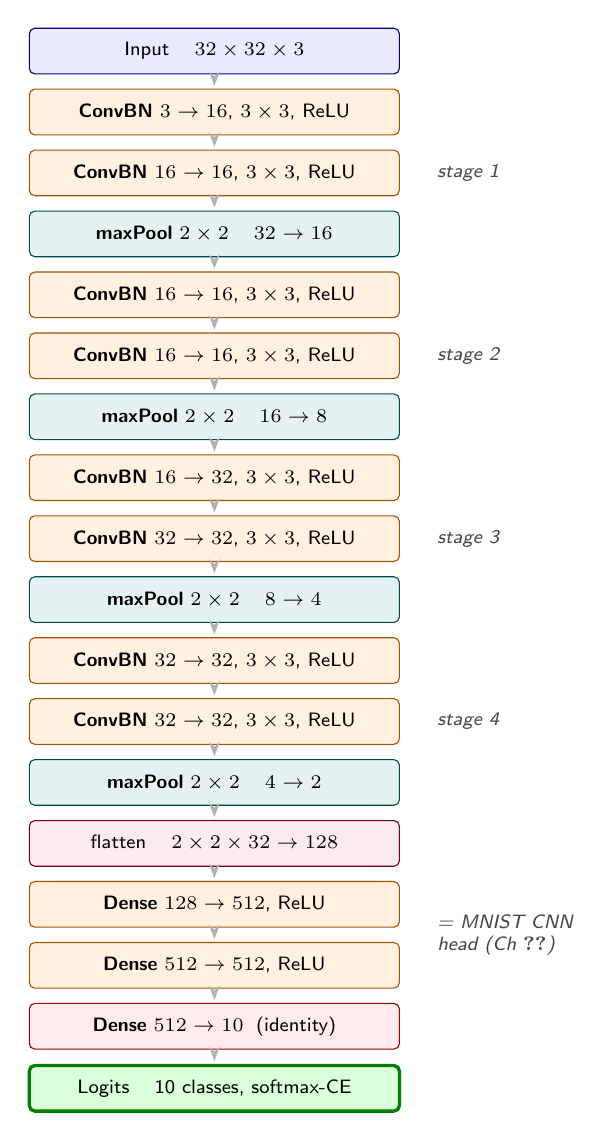
\begin{tikzpicture}[
  >={Stealth[length=1.8mm]},
  every node/.style={font=\sffamily\scriptsize},
  col/.style    = {align=center, rounded corners=2pt, inner sep=2pt, minimum height=0.58cm, minimum width=4.7cm},
  io/.style     = {col, draw=blue!55!black,   fill=blue!8},
  convbn/.style = {col, draw=orange!65!black, fill=orange!12},
  pool/.style   = {col, draw=teal!60!black,   fill=teal!10},
  flat/.style   = {col, draw=purple!60!black, fill=purple!8},
  dense/.style  = {col, draw=orange!65!black, fill=orange!12},
  head/.style   = {col, draw=red!60!black,    fill=red!8},
  logits/.style = {col, draw=green!50!black,  fill=green!14, very thick},
  arr/.style    = {->, thick, gray!60, shorten >=1pt, shorten <=1pt},
  stage/.style  = {font=\sffamily\scriptsize\itshape, gray!55!black, anchor=west},
]
  % Vertical layer column: input at top -> logits at bottom.
  \node[io]                            (input) {Input \;\; $32\times32\times3$};
  \node[convbn, below=0.18cm of input] (c1)   {\textbf{ConvBN} $3\to16$, $3\times3$, ReLU};
  \node[convbn, below=0.18cm of c1]    (c2)   {\textbf{ConvBN} $16\to16$, $3\times3$, ReLU};
  \node[pool,   below=0.18cm of c2]    (p1)   {\textbf{maxPool} $2\times2$ \;\; $32\to16$};
  \node[convbn, below=0.18cm of p1]    (c3)   {\textbf{ConvBN} $16\to16$, $3\times3$, ReLU};
  \node[convbn, below=0.18cm of c3]    (c4)   {\textbf{ConvBN} $16\to16$, $3\times3$, ReLU};
  \node[pool,   below=0.18cm of c4]    (p2)   {\textbf{maxPool} $2\times2$ \;\; $16\to8$};
  \node[convbn, below=0.18cm of p2]    (c5)   {\textbf{ConvBN} $16\to32$, $3\times3$, ReLU};
  \node[convbn, below=0.18cm of c5]    (c6)   {\textbf{ConvBN} $32\to32$, $3\times3$, ReLU};
  \node[pool,   below=0.18cm of c6]    (p3)   {\textbf{maxPool} $2\times2$ \;\; $8\to4$};
  \node[convbn, below=0.18cm of p3]    (c7)   {\textbf{ConvBN} $32\to32$, $3\times3$, ReLU};
  \node[convbn, below=0.18cm of c7]    (c8)   {\textbf{ConvBN} $32\to32$, $3\times3$, ReLU};
  \node[pool,   below=0.18cm of c8]    (p4)   {\textbf{maxPool} $2\times2$ \;\; $4\to2$};
  \node[flat,   below=0.18cm of p4]    (fl)   {flatten \;\; $2\times2\times32 \to 128$};
  \node[dense,  below=0.18cm of fl]    (d1)   {\textbf{Dense} $128\to512$, ReLU};
  \node[dense,  below=0.18cm of d1]    (d2)   {\textbf{Dense} $512\to512$, ReLU};
  \node[head,   below=0.18cm of d2]    (d3)   {\textbf{Dense} $512\to10$ \;(identity)};
  \node[logits, below=0.18cm of d3]    (out)  {Logits \;\; 10 classes, softmax-CE};
  \foreach \a/\b in {input/c1, c1/c2, c2/p1, p1/c3, c3/c4, c4/p2, p2/c5,
                     c5/c6, c6/p3, p3/c7, c7/c8, c8/p4, p4/fl, fl/d1,
                     d1/d2, d2/d3, d3/out}
     \draw[arr] (\a) -- (\b);
  % Stage brackets on the right.
  \node[stage] at ($(c1.east)!0.5!(p1.east) + (0.35,0)$) {stage 1};
  \node[stage] at ($(c3.east)!0.5!(p2.east) + (0.35,0)$) {stage 2};
  \node[stage] at ($(c5.east)!0.5!(p3.east) + (0.35,0)$) {stage 3};
  \node[stage] at ($(c7.east)!0.5!(p4.east) + (0.35,0)$) {stage 4};
  % Bridge cue: the dense head is exactly the MNIST CNN's.
  \node[stage, align=left] at ($(d1.east)!0.5!(d2.east) + (0.35,0)$) {= MNIST CNN\\head (Ch~\ref{chap:cnn})};
\end{tikzpicture}
\end{center}

\noindent The \texttt{ConvBN} boxes are the with-BN variant. The no-BN
net is identical with each \texttt{ConvBN} replaced by a plain
\texttt{Conv2D~+~ReLU}. Both specs are written out next.

\subsection*{The two specs, differing by one keyword per layer}

Eight $3 \times 3$ convolutions in four stages (channel widths
$16, 16, 32, 32$, a max-pool after each stage), then the 2$\times$512
dense head lifted straight from the MNIST CNN. Without BN, each
convolution is followed by a plain ReLU. With
BN, a per-channel BatchNorm sits between the convolution and the ReLU.
That one keyword per conv layer is the entire difference.

Without BN:

\begin{verbatim}
def cifar8wVerified : VerifiedNetSpec where
  name     := "CIFAR-CNN8-wide"
  slug     := "cifar8w"
  inC      := 3
  imageH   := 32
  imageW   := 32
  nClasses := 10
  data     := .cifar
  layers   := [.conv 3 16 3 1, .relu, .conv 16 16 3 1, .relu, .maxPool 2 2,
               .conv 16 16 3 1, .relu, .conv 16 16 3 1, .relu, .maxPool 2 2,
               .conv 16 32 3 1, .relu, .conv 32 32 3 1, .relu, .maxPool 2 2,
               .conv 32 32 3 1, .relu, .conv 32 32 3 1, .relu, .maxPool 2 2,
               .flatten,
               .dense 128 512, .relu, .dense 512 512, .relu, .dense 512 10]
\end{verbatim}

With BN:

\begin{verbatim}
def cifar8wBnVerified : VerifiedNetSpec where
  name     := "CIFAR-CNN8-wide-BN"
  slug     := "cifar8w_bn"
  inC      := 3
  imageH   := 32
  imageW   := 32
  nClasses := 10
  data     := .cifar
  layers   := [.conv 3 16 3 1, .bnPerChannel 16, .relu,
               .conv 16 16 3 1, .bnPerChannel 16, .relu, .maxPool 2 2,
               .conv 16 16 3 1, .bnPerChannel 16, .relu,
               .conv 16 16 3 1, .bnPerChannel 16, .relu, .maxPool 2 2,
               .conv 16 32 3 1, .bnPerChannel 32, .relu,
               .conv 32 32 3 1, .bnPerChannel 32, .relu, .maxPool 2 2,
               .conv 32 32 3 1, .bnPerChannel 32, .relu,
               .conv 32 32 3 1, .bnPerChannel 32, .relu, .maxPool 2 2,
               .flatten,
               .dense 128 512, .relu, .dense 512 512, .relu, .dense 512 10]
\end{verbatim}

The diff is eight \texttt{.bnPerChannel} entries, one inserted between
each convolution and its ReLU. The dense head, the max-pools, and the
training config are all identical.

\paragraph{What \texttt{.bnPerChannel} contributes.} One arm, and the
only new one this chapter needs --- \texttt{.conv}, \texttt{.maxPool},
\texttt{.flatten}, \texttt{.dense} and \texttt{.relu} are all
Chapter~\ref{chap:cnn}'s, unchanged:

\begin{verbatim}
  | bnPerChannel oc => #[(#[oc],1),(#[oc],2)]   -- gamma (ones), beta (zeros)
\end{verbatim}

\noindent This is where \texttt{initKind} stops being bookkeeping.
BatchNorm's $\gamma$ initialises to \emph{ones} and $\beta$ to zeros, so
a freshly built net's BN is the identity and the surrounding
convolutions see exactly what they would have seen without it. Zero-init
$\gamma$ instead and the whole trunk outputs $\beta$ regardless of its
input. Note also what is \emph{not} here: the running mean and variance.
Those are statistics, not parameters --- no gradient reaches them --- which
is why they are threaded separately through \texttt{bnChannels} rather
than living in this list.

\medskip\noindent\textbf{The spec-to-proof tie.} These are
\texttt{VerifiedNetSpec}s, which is what makes the listing above load
bearing rather than descriptive. The \texttt{slug} names the committed
render, so \texttt{cifar8w\_bn} is
\texttt{verified\_mlir/cifar8w\_bn\_\{mom,sgd,adam\}\_train\_step.mlir},
the files the run in \S\ref{sec:bn_runit} handed to XLA. The
\texttt{layers} list folds to a parameter layout through
\texttt{toSpecs}, and a \texttt{\#guard} in the same file pins that
layout against the one the renderer emits, so a spec that drifts from
its render fails the build rather than training something else. The
gradient itself is \texttt{Proofs.cifarCnn8\_has\_vjp\_at}, proved once
and \emph{parametrically in the head width}, which is why the
$512$-wide head here and the $64$-wide one behind \texttt{cifar8-bn-verified}
need no separate proof between them. \texttt{cifarCnn8\_has\_vjp\_at\_correct}
(\texttt{Proofs/Architectures/CifarCNN.lean}) is the statement that its
backward is the derivative, and \texttt{Proofs/Cifar8Close.lean} carries
that through to the emitted training step. Both nets run the same
XLA/PJRT path on the GPU.

\subsection*{Lever 1: normalization}

Fix the optimizer at plain SGD and toggle BN. Both nets train for 40
epochs on the shared pipeline. Per-epoch test accuracy, the median of
five runs each, from the verified runs in
\texttt{runs/2026-08-12-cifar8w-6arm-xla-cuda/}:

\begin{center}
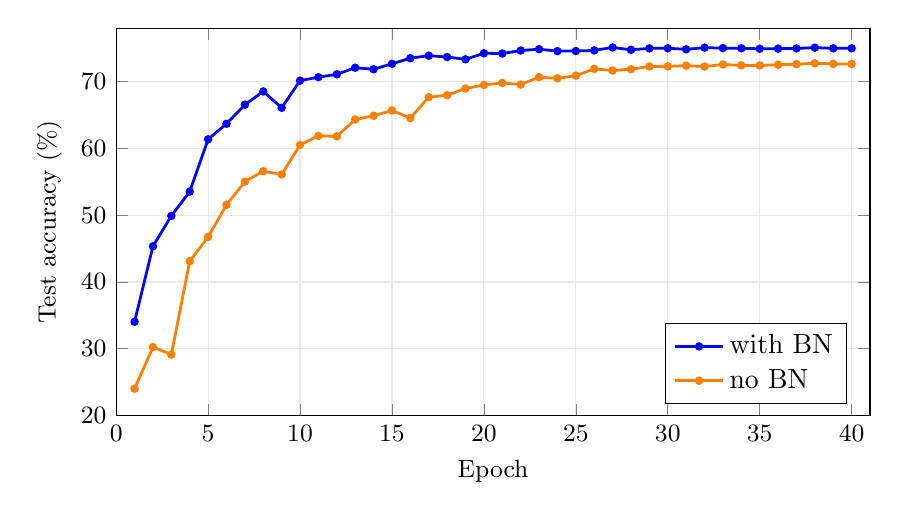
\begin{tikzpicture}
\begin{axis}[
    width=0.92\linewidth, height=6.5cm,
    xlabel={Epoch}, ylabel={Test accuracy (\%)},
    xmin=0, xmax=41, ymin=20, ymax=78,
    xtick={0,5,10,15,20,25,30,35,40},
    ytick={20,30,40,50,60,70},
    legend pos=south east,
    legend cell align={left},
    grid=major, grid style={gray!18},
    tick label style={font=\small},
    label style={font=\small},
    every axis plot/.append style={line width=1pt, mark size=1pt},
]
\addplot[blue, mark=*, mark options={fill=blue}] coordinates {
(1,34.04) (2,45.34) (3,49.90) (4,53.53) (5,61.36) (6,63.69) (7,66.54) (8,68.53) (9,66.08) (10,70.15) (11,70.67) (12,71.10) (13,72.08) (14,71.85) (15,72.67) (16,73.51) (17,73.89) (18,73.69) (19,73.34) (20,74.25) (21,74.21) (22,74.66) (23,74.86) (24,74.57) (25,74.58) (26,74.68) (27,75.12) (28,74.77) (29,74.98) (30,75.00) (31,74.84) (32,75.09) (33,75.02) (34,75.00) (35,74.92) (36,74.94) (37,74.98) (38,75.09) (39,74.99) (40,75.00)
};
\addlegendentry{with BN}
\addplot[orange, mark=*, mark options={fill=orange}] coordinates {
(1,24.01) (2,30.24) (3,29.12) (4,43.11) (5,46.74) (6,51.55) (7,55.02) (8,56.59) (9,56.09) (10,60.52) (11,61.88) (12,61.81) (13,64.33) (14,64.89) (15,65.68) (16,64.54) (17,67.67) (18,67.97) (19,68.97) (20,69.50) (21,69.81) (22,69.56) (23,70.67) (24,70.49) (25,70.89) (26,71.91) (27,71.67) (28,71.86) (29,72.27) (30,72.29) (31,72.40) (32,72.26) (33,72.57) (34,72.43) (35,72.43) (36,72.53) (37,72.61) (38,72.75) (39,72.66) (40,72.64)
};
\addlegendentry{no BN}
\end{axis}
\end{tikzpicture}
\end{center}

\noindent CIFAR-10, wide 8-conv net, plain SGD (lr~0.1,
cosine${+}$warmup) on the shared pipeline, 40 epochs, BN vs no-BN,
through the verified renderer. Median of $n{=}5$ runs per curve. The
final points span $74.5$ to $75.6$ with BN and $71.6$ to $73.4$
without (\texttt{runs/2026-08-12-cifar8w-6arm-xla-cuda/}, the SGD phase).

\noindent BN leads from the first epoch, 34\% to the bare net's
24\%, and keeps the lead the whole way, finishing about two and a half
points up (75.0\% vs 72.6\%). The un-normalized net traces the same arc
roughly ten epochs behind. Most of that is \emph{speed}, since the curves
are the same shape shifted left, but at this depth on plain SGD it is
also a real convergence margin, and it is larger than the run-to-run
spread on either curve. The conditioning that the three-term
backward (\S\ref{thm:bnNormalize_has_vjp}) buys is worth more the deeper
the stack, exactly the trend that makes BN standard equipment by
ResNet's thirty-four layers. Under momentum and AdamW, next, the
un-normalized net trains fast enough to close most of the accuracy gap,
and pays for it in a way plain SGD never exposed.

\subsection*{Lever 2: the optimizer}

Now hold the architecture fixed and change only the update rule. Three
optimizers, each at its own tuned learning rate, all on the identical
pipeline and the same 40 epochs. Median final accuracy, with the
observed range across runs:

\begin{center}
\begin{tabular}{l c c c}
\hline
       & SGD & momentum & AdamW \\
       & (lr 0.1) & ($\mu$ 0.9, lr 0.02) & (lr $10^{-3}$) \\
\hline
no BN  & 72.6 {\footnotesize (1.8)} & \emph{diverged} & 73.7 {\footnotesize (1.0)} \\
BN     & 75.0 {\footnotesize (1.1)} & \textbf{77.1} {\footnotesize (0.8)} & 74.4 {\footnotesize (0.8)} \\
\hline
\end{tabular}
\end{center}

\noindent $n=5$ per cell, $n=4$ for the AdamW column. Parenthesised
figures are the range from lowest run to highest.

\noindent Momentum with BN is the best result on the board at 77.1\%,
about two points over plain SGD and two and a half over AdamW, and every
one of those gaps is wider than the spread within a cell. AdamW lands
between the two: its per-coordinate second-moment scaling is worth
something over plain SGD, but less than momentum is, even with the wide
head's extra parameters to exploit. Reading \emph{down} the columns
recovers Lever~1, and BN is ahead in all three ($+2.4$ under SGD,
$+0.7$ under AdamW, and under momentum the comparison does not finish).

\medskip\noindent\textbf{The empty cell is the finding.} Un-normalized
plus momentum did not fail to reach a good accuracy. It reached one and
then destroyed it. In all five runs the training loss fell normally to
about $0.27$ and then went to \texttt{NaN} between epochs 29 and 34, at a
learning rate the cosine schedule had already decayed to roughly
$0.002$. Three of the five collapsed to 10\% by epoch 40, which is chance
on ten classes. The other two happened to be evaluated before the damage
propagated and still reported about 76\%. There is no honest single
number for that cell, so the table does not print one. The same thing
happened once in four AdamW runs without BN. Across all fourteen
un-normalized runs the loss went to \texttt{NaN} six times, and across
all fourteen normalized ones it never did.

\noindent That is the sharper version of Lever~1. On plain SGD, BN buys
speed and a couple of points. Give the net a stronger optimizer and BN
stops looking like an accelerator and starts looking like the thing
holding the net together, which is what deep normalization is actually
for. It is the same instability an eight-layer stack without
normalization has always been prone to, and it is why the next chapter's
thirty-four layers do not attempt it.

\medskip\noindent The Lever-1 graph drew this for the SGD column, with
the optimizer fixed and BN toggled. The same per-epoch picture for the
other two columns, on the same axes, is what reading \emph{down} the
table looks like drawn out:

\begin{center}
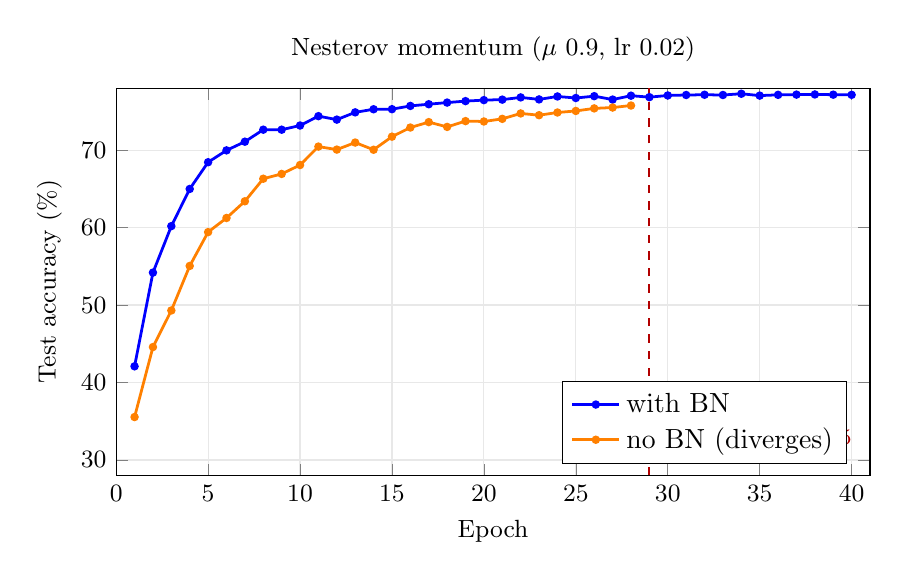
\begin{tikzpicture}
\begin{axis}[
    width=0.92\linewidth, height=6.5cm,
    title={Nesterov momentum ($\mu$ 0.9, lr 0.02)},
    title style={font=\small},
    xlabel={Epoch}, ylabel={Test accuracy (\%)},
    xmin=0, xmax=41, ymin=28, ymax=78,
    xtick={0,5,10,15,20,25,30,35,40},
    ytick={30,40,50,60,70},
    legend pos=south east,
    legend cell align={left},
    grid=major, grid style={gray!18},
    tick label style={font=\small},
    label style={font=\small},
    every axis plot/.append style={line width=1pt, mark size=1pt},
]
\addplot[blue, mark=*, mark options={fill=blue}] coordinates {
(1,42.09) (2,54.19) (3,60.19) (4,64.99) (5,68.44) (6,69.97) (7,71.09) (8,72.64) (9,72.64) (10,73.18) (11,74.39) (12,73.94) (13,74.88) (14,75.28) (15,75.29) (16,75.71) (17,75.93) (18,76.14) (19,76.33) (20,76.46) (21,76.52) (22,76.81) (23,76.55) (24,76.93) (25,76.73) (26,76.97) (27,76.53) (28,77.03) (29,76.84) (30,77.06) (31,77.12) (32,77.15) (33,77.12) (34,77.28) (35,77.04) (36,77.14) (37,77.17) (38,77.19) (39,77.16) (40,77.14)
};
\addlegendentry{with BN}
\addplot[orange, mark=*, mark options={fill=orange}] coordinates {
(1,35.54) (2,44.58) (3,49.30) (4,55.05) (5,59.42) (6,61.24) (7,63.40) (8,66.31) (9,66.93) (10,68.08) (11,70.46) (12,70.07) (13,70.98) (14,70.05) (15,71.74) (16,72.92) (17,73.62) (18,73.00) (19,73.75) (20,73.70) (21,74.04) (22,74.74) (23,74.51) (24,74.86) (25,75.06) (26,75.39) (27,75.50) (28,75.76)
};
\addlegendentry{no BN (diverges)}
\addplot[red!70!black, dashed, line width=0.8pt, forget plot, mark=none]
  coordinates {(29,28) (29,78)};
\node[anchor=south west, font=\footnotesize, red!70!black, align=left]
  at (axis cs:29.4,30) {loss $\to$ \texttt{NaN}\\epochs 29--34, 5/5};
\end{axis}
\end{tikzpicture}
\end{center}

\begin{center}
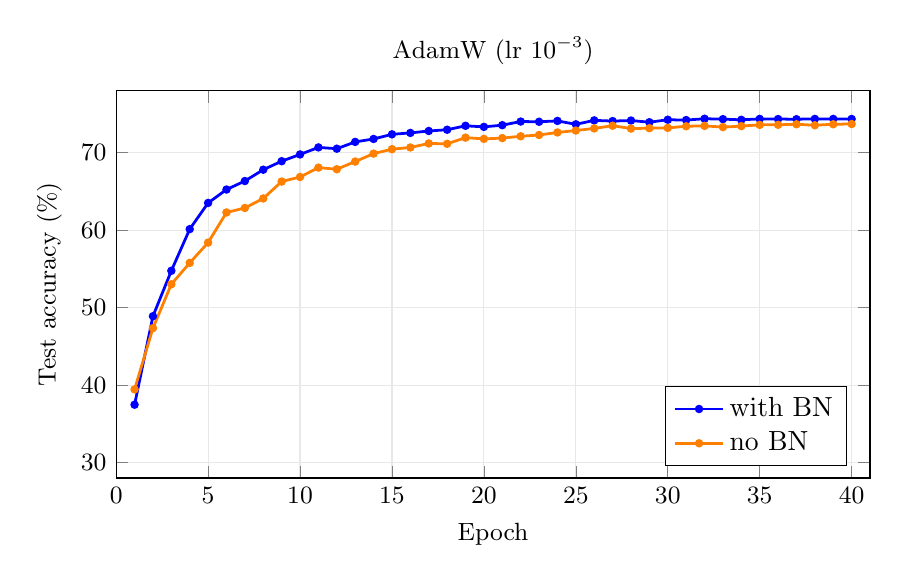
\begin{tikzpicture}
\begin{axis}[
    width=0.92\linewidth, height=6.5cm,
    title={AdamW (lr $10^{-3}$)},
    title style={font=\small},
    xlabel={Epoch}, ylabel={Test accuracy (\%)},
    xmin=0, xmax=41, ymin=28, ymax=78,
    xtick={0,5,10,15,20,25,30,35,40},
    ytick={30,40,50,60,70},
    legend pos=south east,
    legend cell align={left},
    grid=major, grid style={gray!18},
    tick label style={font=\small},
    label style={font=\small},
    every axis plot/.append style={line width=1pt, mark size=1pt},
]
\addplot[blue, mark=*, mark options={fill=blue}] coordinates {
(1,37.47) (2,48.90) (3,54.76) (4,60.14) (5,63.52) (6,65.25) (7,66.35) (8,67.81) (9,68.91) (10,69.78) (11,70.69) (12,70.52) (13,71.40) (14,71.78) (15,72.38) (16,72.56) (17,72.81) (18,72.97) (19,73.48) (20,73.34) (21,73.56) (22,74.03) (23,74.00) (24,74.11) (25,73.67) (26,74.18) (27,74.09) (28,74.16) (29,73.94) (30,74.26) (31,74.22) (32,74.39) (33,74.34) (34,74.25) (35,74.37) (36,74.35) (37,74.33) (38,74.37) (39,74.37) (40,74.36)
};
\addlegendentry{with BN}
\addplot[orange, mark=*, mark options={fill=orange}] coordinates {
(1,39.45) (2,47.36) (3,53.02) (4,55.78) (5,58.40) (6,62.29) (7,62.87) (8,64.10) (9,66.28) (10,66.87) (11,68.08) (12,67.87) (13,68.86) (14,69.89) (15,70.46) (16,70.68) (17,71.20) (18,71.15) (19,71.95) (20,71.79) (21,71.89) (22,72.13) (23,72.29) (24,72.62) (25,72.87) (26,73.14) (27,73.49) (28,73.12) (29,73.17) (30,73.21) (31,73.42) (32,73.47) (33,73.31) (34,73.44) (35,73.60) (36,73.61) (37,73.68) (38,73.55) (39,73.68) (40,73.71)
};
\addlegendentry{no BN}
\end{axis}
\end{tikzpicture}
\end{center}

\noindent Same wide 8-conv net, same shared pipeline, same 40 epochs, and
only the optimizer changes from the SGD panel above
(\texttt{runs/2026-08-12-cifar8w-6arm-xla-cuda/}, the momentum and AdamW
phases). Medians as before, over the runs that finished.

\noindent Under \textbf{momentum} BN takes the early lead, 42\% to
36\% at epoch~1, and the un-normalized net spends the next twenty-five
epochs closing it, reaching $75.8$ against BN's $77.0$ by epoch~28. Then
it stops. The orange curve ends where it does because the training loss
went to \texttt{NaN} in every one of the five runs between epochs 29 and
34, and there is nothing after that worth plotting. Under \textbf{AdamW}
both nets run the full forty epochs, BN ahead by about seven tenths the
whole way ($74.4$ vs $73.7$), which is inside the run-to-run spread and
is not a gap the text ranks. One of the four un-normalized AdamW runs
also went to \texttt{NaN}.

\noindent Read top-to-bottom, SGD then momentum then AdamW, the accuracy
gap between the curves does narrow panel by panel, exactly the old
``BN helps most under a weak optimizer'' reading. The momentum panel is
where that reading breaks. The gap narrows right up to the point the
un-normalized net destroys itself, which means the two curves converging
was never evidence that BN had stopped mattering.

The reason we can make this comparison \emph{and trust it} is that the
optimizer is one swappable rendered tail. The forward pass, the
softmax--cross-entropy loss, the backward pass, and every parameter
gradient are the same proof-rendered graph in each column. Only the
final per-parameter update op changes:

\begin{itemize}
  \item \textbf{SGD}: $\theta \leftarrow \theta - \mathrm{lr}\cdot g$.
  \item \textbf{Momentum (Nesterov)}: $v \leftarrow \mu v + g$, then
    $\theta \leftarrow \theta - \mathrm{lr}\,(\mu v + g)$.
  \item \textbf{AdamW}: the bias-corrected first/second-moment step,
    rendered op-for-op as \texttt{Proofs.adamWParam}.
\end{itemize}

\noindent Each tail is emitted onto the \emph{same} certified gradient
(\texttt{emitSgd}, \texttt{emitMomentum}, \texttt{ViTRender.emitAdamV}),
so the ablation is honest in the strong sense: identical, machine-checked
gradients with different arithmetic stacked on top. And for plain
SGD, that the binary32 step actually decreases the loss is itself a
proved theorem.

\noindent It is worth being precise about what that does and does not
cover, because the momentum column just exercised the gap. The proofs
say the emitted graph computes the gradient this chapter derives, and
they say it in exact real arithmetic. They say nothing about whether
forty epochs of binary32 updates stay in range. A verified gradient is
not a guarantee of numerical stability, and the un-normalized momentum
run is what that distinction looks like when it bites.

\medskip\noindent\textbf{One honest note on the comparison.} The first
time we ran this, the optimizers looked far more separated, with momentum
and Adam beating SGD by some ten points. That gap was mostly an artifact:
the momentum and Adam runs happened to go through a data pipeline with
shuffling and flip augmentation that the plain-SGD baseline lacked.
Holding the pipeline genuinely fixed, as the table above does, collapsed
the difference to the few points that are really about the
optimizer. It is exactly the kind of mistake a verified gradient does
\emph{not} catch. The math was correct in every run, and the experiment
design was what needed fixing. An ablation measures the thing you varied
only if everything else is held constant, and ``everything else''
includes the parts that live outside the network.

\subsection*{Lever 3: the arithmetic}

Levers 1 and 2 changed the \emph{network} and the \emph{update rule}. This one
changes neither. It holds both fixed and changes only the number format the
convolutions are computed in, which is the sharpest version of the chapter's
question: if the optimizer ranking is a fact about optimization, it should
survive being computed in a different arithmetic.

Three precisions, the same three optimizers, the same 40 epochs and the same
pipeline. Median of five runs, with the observed range:

\begin{center}
\begin{tabular}{l c c c}
\hline
          & fp32 & bf16 & fp8 (E4M3) \\
\hline
SGD (lr 0.1)          & 72.6 {\footnotesize (1.2)} & 72.5 {\footnotesize (2.6)} & 72.2 {\footnotesize (3.3)} \\
AdamW (lr $10^{-3}$)  & 74.3 {\footnotesize (2.3)} & 73.9 {\footnotesize (2.1)} & 74.3 {\footnotesize (1.5)} \\
momentum ($\mu$ 0.9)  & \emph{diverged} & \emph{diverged} & \emph{diverged} \\
\hline
\end{tabular}
\end{center}

\noindent $n=5$ per cell. Reading \emph{down} each column recovers Lever~2, and
it recovers it three times: SGD is last, AdamW is second, momentum is first, in
every arithmetic. \textbf{The ranking is invariant.} Reading \emph{across} the
rows, the medians agree to within half a point --- 72.6/72.5/72.2 and
74.3/73.9/74.3 --- which is well inside the spread \emph{within} a single cell.
Sixteen-bit and eight-bit arithmetic land on the same curve as fp32.

\medskip\noindent\textbf{The whole momentum row is Lever~1 again, and the
accuracies are what mislead.} In \emph{all three} arithmetics, every one of the
five momentum runs sent its training loss to \texttt{NaN} --- fifteen runs out of
fifteen. Only two of them had visibly collapsed to 10\% by the time epoch~40 was
evaluated; the other thirteen still reported something around 76\%, which is
precisely the trap Lever~2 warns about, and precisely why the loss and not the
accuracy is the thing to read. Had we scored this row on test accuracy alone, we
would have printed a best-in-table 76.0 for bf16 and called it a win.

\noindent That the failure is identical across fp32, bf16 and fp8 is the point.
The un-normalized eight-layer stack with momentum is unstable as a
\emph{network}; the number format neither causes it nor cures it. Reduced
precision is being blamed for nothing here, and credited with nothing either.

\noindent AdamW is a milder version of the same story: two of five fp32 runs and
one of five in each low-precision column touch \texttt{NaN} without ever
collapsing, matching the ``once in four'' Lever~2 saw. Plain SGD is clean in all
fifteen runs. So the ordering the table reports rests on the two rows that
finish healthy, and the third row is reported as diverged rather than scored.

\medskip\noindent\textbf{What the two low-precision columns actually are}, since
they are not the same kind of object. The bf16 arm is genuine reduced precision
\emph{in the graph}: all twenty-three convolutions of the training step --- the
forward, the input gradient and the weight gradient --- carry bf16 operands and a
bf16-typed result, and only the parameter updates stay in fp32. The fp8 arm is
\emph{emulated}: weights and inputs are projected onto the E4M3 grid, but the
graph itself is fp32 and accumulation is fp32. It is the right arithmetic and
the wrong hardware path, which is enough for a statement about numerics and not
enough for one about speed.

\medskip\noindent\textbf{And there is no speed claim here.} At this network's
size the convolutions are launch-bound --- sixteen to thirty-two channels on
grids from $32^2$ down to $4^2$ --- so the tensor cores that make bf16 and fp8
worth having on ImageNet-scale models sit idle. Measured directly, bf16 runs at
$0.87\times$ fp32 across this conv stack: slightly \emph{slower}. The payoff for
low precision is a story about ResNet-34 and beyond (Ch~\ref{chap:residual});
what CIFAR can show is that the mathematics survives the trip, and that is what
this lever is for.

\subsection*{Does the head width matter?}

Almost not at all, which is exactly why we could borrow MNIST's head
untouched. The 2$\times$512 head carries about $334{,}000$ of the net's
$374{,}000$ parameters. Swap it for a narrow 64-wide head ($13{,}000$
params, whole net down to $53{,}000$) and the best cell on the board
barely moves: BN with momentum gives $77.1\%$ wide against $77.1\%$
narrow, and the optimizer ordering is unchanged. Seven times the
parameters buys no accuracy, and costs about $1.6\times$ the wall-clock
per epoch (${\approx}6.3$ vs ${\approx}3.9$ seconds on an RTX 4060 Ti).
The eight convolutions over the $32 \times 32$ maps dominate the compute,
while the head is cheap matmul however big it is. That is the lesson the
bridge makes concrete: at this scale the \emph{depth} of the
convolutional body is the lever, not the width of the classifier on top.
It is why the head can stay MNIST's, and why the next chapter spends its
budget on thirty-four layers of \emph{more convolution} rather than a
bigger head.

The two-point comparison above (64 vs 512) is worth drawing out in full,
because the parametric renderer makes it cheap: \texttt{cifar8-bn-grid}
holds the eight-convolution backbone fixed and renders the AdamW train step
at any head width $d$ (the same $D_1$ that was hard-wired to 64 is now a
parameter of the verified emitter), so we can sweep $d$ from 8 to 4096 and
train each point on its own proof-rendered StableHLO. Split across the two
gfx1100s, the whole curve is one short run:

\begin{center}
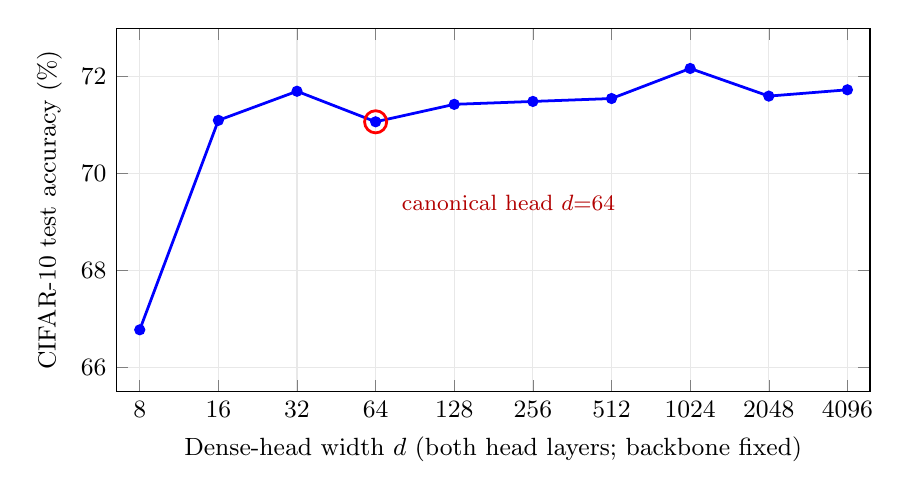
\begin{tikzpicture}
\begin{axis}[
    width=0.92\linewidth, height=6.2cm,
    xlabel={Dense-head width $d$ (both head layers; backbone fixed)},
    ylabel={CIFAR-10 test accuracy (\%)},
    xmode=log, log basis x=2,
    xmin=6.5, xmax=5000, ymin=65.5, ymax=73,
    xtick={8,16,32,64,128,256,512,1024,2048,4096},
    xticklabels={8,16,32,64,128,256,512,1024,2048,4096},
    ytick={66,68,70,72},
    grid=major, grid style={gray!18},
    tick label style={font=\small},
    label style={font=\small},
    every axis plot/.append style={line width=1pt, mark size=1.5pt},
]
\addplot[blue, mark=*, mark options={fill=blue}] coordinates {
(8,66.78) (16,71.10) (32,71.70) (64,71.07) (128,71.43) (256,71.49) (512,71.55) (1024,72.17) (2048,71.60) (4096,71.73)
};
\addplot[only marks, mark=o, mark size=4pt, red, line width=1pt, forget plot] coordinates {(64,71.07)};
\node[anchor=west, font=\footnotesize, red!70!black] at (axis cs:74,69.4)
  {canonical head $d{=}64$};
\end{axis}
\end{tikzpicture}
\end{center}

\noindent Dense-head width sweep for the 8-conv cifar8 net with per-channel
BatchNorm, AdamW, 25 epochs, conv backbone held at $[16,16,32,32]$
(\texttt{runs/cifar8bn\_grid\_results.tsv}). Past a 16-wide head the curve is
essentially flat, and everything from $d{=}16$ to $d{=}4096$ lands inside a
single point ($71.1$ to $72.2\%$), and the $256\times$ wider head buys
nothing, while its $17$M-parameter classifier just overfits (train loss
$0.03$, test unmoved). The only real drop is at $d{=}8$ ($66.8\%$), where the
$128{\to}8$ first layer throttles the 128-dim feature map the convolutions
produce. The canonical $d{=}64$ (circled) sits squarely on the plateau: the
head width genuinely does not matter here, which is the whole reason the net
could borrow MNIST's classifier untouched. (Absolute accuracy is a couple of
points below the 40-epoch board above, because this is a 25-epoch
single-optimizer sweep, but the \emph{shape} is the point.)

\subsection*{Why the levers work}

Both levers do the same underlying thing by attacking different sources
of noise. They make each step's gradient a more reliable guide to the
next. Each layer is tuned for the distribution of its
inputs, but those inputs are the outputs of every layer below, which
shift every step, so each layer chases a moving target, and the step
that helps one layer can wreck the next. \textbf{BN} removes the moving
part by pinning every layer's input to mean-zero, unit-variance before
the learnable $\gamma,\beta$ get a say. Ioffe \& Szegedy framed this
as reducing ``internal covariate shift,'' while Santurkar et al.\ (2018)
argued the sharper effect is a smoother loss landscape.
\textbf{Momentum} attacks a different noise: by averaging successive
gradients it cancels the mini-batch jitter and accumulates the
consistent direction. Both make the per-step direction more trustworthy,
and reliable progress compounds across epochs, which is what the
curves and the table measure.

The two levers interact, and the momentum column is where that shows.
Momentum makes each step longer and more consistent, which is why it wins
on accuracy, and a longer step through eight unnormalized layers is also
exactly what runs the activations out of binary32 range. Normalization is
what makes the aggressive optimizer survivable. That is the standard
account of why the two arrived together, and why every image architecture
since 2015 bakes a normalization layer in by default. At larger depth
the effect is stronger still, and it is what opens up the learning rates
that diverge without it. Between them the two levers decide not only how
many passes the net needs, but whether it finishes them at all.

\section{MLIR: BatchNorm}

\noindent\textbf{What is already proven.} BatchNorm factors as
$\mathrm{bnForward} = \mathrm{bnAffine} \circ \mathrm{bnNormalize}$, and its
reverse-mode derivative is the three-term formula of
\S~\ref{thm:bnNormalize_has_vjp}: with $\hat{x} = (x-\mu)\,\mathrm{istd}$,
\[
  dx = \frac{\mathrm{istd}\,\gamma}{n}\Bigl(n\,dy
       \;-\; \textstyle\sum_k dy_k
       \;-\; \hat{x}\,\textstyle\sum_k \hat{x}_k\,dy_k\Bigr).
\]
\texttt{bn\_has\_vjp} proves it, composing \texttt{bnNormalize\_has\_vjp}
(the rank-1 wringer) with \texttt{bnAffine\_has\_vjp} (the $\gamma\,dy$
half). The one subtlety, isolated in \S~\ref{ax:bnIstdBroadcast_diff}, is
that the inverse-stddev term carries an $\mathrm{istd}^3$ that needs
$\varepsilon > 0$ to stay differentiable. That is the single place in the
book where the math reaches past chain-sum-product into real analysis.

\medskip\noindent\textbf{The gap and how we close it.} The three-term
backward is not elementwise, because the two $\sum_k$ reductions couple
every coordinate to every other. The emitted backward graph is given a
denotation in the proofs' own vector type, and
\texttt{bn\_back\_bridge} proves that denotation equal to
\texttt{bn\_has\_vjp}'s backward. The emitted reduce/broadcast/elementwise
graph \emph{is}, by machine check, the three-term formula. Here is what the
printer emits, with the forward-statistic recompute (mean, variance,
\texttt{rsqrt}, normalize) elided to its one comment line, at $n=4$:

\begin{verbatim}
// forward stats recomputed: %mu, %istd, %xhat = (x-mu)*istd
%dxhat = stablehlo.multiply %gb, %dy : tensor<2x4xf32>   // dxhat = g*dy
%sdx_r = stablehlo.reduce(%dxhat init: %sc)
           applies stablehlo.add across dimensions = [1]
           : (tensor<2x4xf32>, tensor<f32>) -> tensor<2xf32>
%sdx = stablehlo.broadcast_in_dim %sdx_r, dims = [0]
           : (tensor<2xf32>) -> tensor<2x4xf32>          // sum dxhat
%xd = stablehlo.multiply %xhat, %dxhat : tensor<2x4xf32>
%sxdx_r = stablehlo.reduce(%xd init: %sc)
           applies stablehlo.add across dimensions = [1]
           : (tensor<2x4xf32>, tensor<f32>) -> tensor<2xf32>
%sxdx = stablehlo.broadcast_in_dim %sxdx_r, dims = [0]
           : (tensor<2xf32>) -> tensor<2x4xf32>          // sum xhat*dxhat
%t1 = stablehlo.multiply %dxhat, %nf : tensor<2x4xf32>   // N*dxhat
%i1 = stablehlo.subtract %t1, %sdx : tensor<2x4xf32>     //   - sum dxhat
%xs = stablehlo.multiply %xhat, %sxdx : tensor<2x4xf32>
%i2 = stablehlo.subtract %i1, %xs : tensor<2x4xf32>      //   - xhat*(sum)
%s = stablehlo.divide %istd, %nf : tensor<2x4xf32>       // istd/N
%dx = stablehlo.multiply %s, %i2 : tensor<2x4xf32>
return %dx : tensor<2x4xf32>
\end{verbatim}

\noindent Read it against the formula. \texttt{\%dxhat} is the affine
backward $\gamma\,dy$, and each \texttt{reduce} along \texttt{dimensions = [1]}
followed by a \texttt{broadcast\_in\_dim} is one of the cross-coordinate
sums ($\sum_k dy_k$ as \texttt{\%sdx}, $\sum_k\hat{x}_k\,dy_k$ as
\texttt{\%sxdx}). \texttt{\%i1} assembles $n\,dy - \sum dy$ (the direct term
minus the centering correction), \texttt{\%i2} subtracts the rank-1
normalization correction $\hat{x}\sum\hat{x}\,dy$, and \texttt{\%dx} scales
the whole bracket by $\mathrm{istd}/n$. The graph folds $\gamma$ into
\texttt{\%dxhat} up front, which is why that leading scale is
$\mathrm{istd}/n$ and not $\mathrm{istd}\,\gamma/n$. It is the same
formula with $\gamma$ pulled inside the parenthesis. The bridge theorem is
precisely the claim that this text computes \texttt{bn\_has\_vjp}'s backward.

\medskip\noindent Because LayerNorm is BatchNorm along a different axis, the
very same emitted graph denotes the LayerNorm backward
(\texttt{layernorm\_back\_bridge} is literally \texttt{bn\_back\_bridge}).
That is the normalization sitting inside the residual, depthwise, and
ConvNeXt blocks built on this foundation.

\medskip\noindent\textbf{Caveats.}
\begin{itemize}
  \item \textbf{Needs $\varepsilon > 0$.} The inverse-stddev term carries an
    $\mathrm{istd}^3$. Given $\varepsilon > 0$ the bridge is unconditional
    (smooth everywhere, with no smooth-point exclusion, unlike ReLU and
    max-pool).
  \item \textbf{Representative scale} ($n = 4$).
\end{itemize}

The next chapter (\S~\ref{chap:residual}) adds residual connections
and the same mechanical approach: prove that the VJP of a skip
connection is additive fan-in, compose with BN and conv, and the
rest of the ResNet family falls out without introducing any new
math.

\chapter{ResNet-34}
\label{chap:residual}

\prosesection{Deeper networks used to stop training}

Before 2015, the dominant assumption in image classification was
``deeper is better, up to a point.'' The ``up to a point'' part was
not metaphorical. If you took a 20-layer CNN that trained to 70\%
val accuracy and added 12 more convolutional layers, you didn't
get a 32-layer model with 72\% accuracy. You got a 32-layer model
that, after the same training budget, fit the \emph{training set}
worse than the 20-layer one did. The 32-layer model had strictly
more capacity. It still trained worse. Something about deep stacks
of convolutions made gradient flow degrade in a way that the
optimizer couldn't navigate around.

He et al.\ 2015
(\href{https://arxiv.org/abs/1512.03385}{arXiv:1512.03385}) had the
right observation: if the
12 extra layers in the deeper network were \emph{initialized to
compute the identity}, the 32-layer network would have at least
the 20-layer's performance, because it could replicate it
exactly. So the question was not ``can a deep network represent
what a shallow one represents?'' It provably could. The question
was: why is optimizing 12 free-form layers to recover identity
so much harder than just leaving identity there?

\section{Run it first}
\label{sec:r34_runit}

Before any of the math, train the thing. Four commands and about an hour
and a half of GPU time:

\begin{verbatim}
lake exe cache get                            # Mathlib oleans, ~30 s
./download_imagenette.sh                      # 330 MB dl, 2.4 GB unpacked
lake build resnet34-verified-adam
./.lake/build/bin/resnet34-verified-adam data
\end{verbatim}

On one RTX 4060 Ti (CUDA 12.9), from
\texttt{runs/2026-08-12-r34-imagenette-xla-cuda/}. XLA's startup banner is
removed, the network description line is wrapped, and epochs 5 through 75
are elided:

\begin{verbatim}
[pjrt_ffi] XLA backend: PJRT 0.112, 1 device(s)
[pjrt_ffi] compiled verified_mlir/resnet34_adam_train_step.mlir
             (@resnet34_adam_train_step, 405 outputs, 1 replica) in 4952 ms
[pjrt_ffi] compiled verified_mlir/resnet34_fwd.mlir
             (@resnet34_fwd, 1 outputs, 1 replica) in 409 ms
[pjrt_ffi] compiled verified_mlir/resnet34_fwd_eval.mlir
             (@resnet34_fwd_eval, 1 outputs, 1 replica) in 195 ms
Real ResNet-34 on Imagenette 224² (7×7-s2 stem→3×3-s2 overlapping max pool→
  [3,4,6,3] blocks w/ batch-norm, He et al. option-B 1×1 projection shortcuts,
  no conv biases; 56→28→14→7→GAP→dense)
  via the VERIFIED renderer → XLA/PJRT → GPU
  train 9469, val 3925; bs 32, ResNet-34 adam
    (cosine+warmup 3ep, baseLR 0.001000), He init
  running-stats BN: 36 layers, 17024 stat floats → eval via @resnet34_fwd_eval
Epoch 1/80: loss=2.049761 lr=0.000333
  epoch 1: val_acc = 1083/3925 = 27.592357%  top5 = 2601/3925 = 66.267516%
Epoch 2/80: loss=1.530066 lr=0.000667
  epoch 2: val_acc = 1363/3925 = 34.726115%  top5 = 3024/3925 = 77.044586%
Epoch 3/80: loss=1.388131 lr=0.001000
  epoch 3: val_acc = 2250/3925 = 57.324841%  top5 = 3554/3925 = 90.547771%
Epoch 4/80: loss=1.300556 lr=0.001000
  epoch 4: val_acc = 2510/3925 = 63.949045%  top5 = 3642/3925 = 92.789809%
Epoch 76/80: loss=0.502019 lr=0.000007
  epoch 76: val_acc = 3522/3925 = 89.732484%  top5 = 3858/3925 = 98.292994%
Epoch 79/80: loss=0.502105 lr=0.000000
  epoch 79: val_acc = 3522/3925 = 89.732484%  top5 = 3857/3925 = 98.267516%
Epoch 80/80: loss=0.502114 lr=0.000000
  epoch 80: val_acc = 3521/3925 = 89.707006%  top5 = 3857/3925 = 98.267516%
done (trained ResNet-34 adam + cosine/warmup via packed threading).
\end{verbatim}

Eighty epochs at about 65 seconds each, roughly an hour and a half in total,
and \textbf{89.71\%} top-1 with \textbf{98.27\%} top-5 on Imagenette's
3,925-image validation split. The best epoch reached $89.86\%$. That is a
thirty-four-layer network trained from scratch on ten thousand photographs,
which is a different kind of problem from the handwritten digits three
chapters back.

Thirty-four layers on, nothing about the claim has changed. That run did
not execute a reimplementation of
the network this chapter describes. It executed
\texttt{verified\_mlir/resnet34\_adam\_train\_step.mlir}, which is
\texttt{pretty(provenGraph)} off the renderer, and every one of the sixteen
residual blocks in it computes the additive fan-in backward that
Theorem~\ref{thm:residual_has_vjp} proves. The thirty-six BatchNorms compute the
three-term backward of Chapter~\ref{chap:bn}, and the convolutions compute the
backward of Chapter~\ref{chap:cnn}. Every theorem in the rest of this chapter is
about the graph that just trained.

Three compile lines rather than the two earlier chapters showed, and the third
is the interesting one. \texttt{@resnet34\_fwd\_eval} is a \emph{separate}
forward, because BatchNorm behaves differently at training time than at
evaluation time. Training normalizes each batch by its own statistics, while
evaluation has to use the running averages accumulated over training, and the
line \texttt{running-stats BN: 36 layers, 17024 stat floats} is the driver
saying it is threading those averages out of the train step and into the eval
forward. A net that skips this reports chance forever, since the eval forward
normalizes by statistics nobody ever computed.

The final loss settles at $0.502$ and stops. That is not the optimizer giving
up. It is the label-smoothing floor derived in \S\ref{sec:r34_recipe}: with
$\varepsilon = 0.1$ over ten classes the smallest attainable cross-entropy is
about $0.485$, so a run that lands at $0.502$ has essentially converged.

\prosesection{The residual block: ask for the difference, not the function}

Their fix was a one-line architectural change. Instead of asking
each block to learn a function \(y = f(x)\), ask it to learn a
function \(y = f(x) + x\). The block's job is no longer to
\emph{become} the new representation. Its job is to learn what to
\emph{add} to the current representation. At initialization, with
randomly-small \(f\), each block is approximately the identity,
and a stack of 16 such blocks is approximately a stack of
16 identities, which is to say, approximately the input. The
network starts out near-identity at every depth and only gradually
takes on structure as \(f\) trains. The optimization problem
becomes ``what residual should each block add'' instead of ``what
function should each block be,'' and the former turns out to be
dramatically easier.

The change to the architecture is one \texttt{+} sign. The change
to the training dynamics is the difference between ``18 layers is
about as deep as we can go'' and ``152 layers trains stably, so let
us also add another zero on the ImageNet leaderboard.''

\prosesection{Why the proof is a one-liner}

From the framework's perspective, what is a residual block?
\(\mathrm{residual}(x) = f(x) + \mathrm{id}(x)\), a sum of two
functions sharing the same input. We already proved in
Chapter~\ref{chap:tensor} that the VJP of an additive fan-in is
``send the upstream gradient through both branches and add.'' We
already proved that the VJP of \(\mathrm{id}\) is the identity on
the gradient (and that the VJP of \(f\) is whatever the inner
block's machinery gives us). Composition is just
\(\mathrm{vjp\_comp}\). So the residual VJP is the additive
fan-in lemma, with \(\mathrm{id}\) plugged into one slot.

That is Theorem~\ref{thm:residual_has_vjp} below, and its proof
is one line. This chapter has \emph{exactly one theorem}, and
that theorem is mechanical. The engineering revolution was not
in the math. It was in the realization that this
operation was the missing piece for training deep
networks. The fact that the framework absorbs the new
architecture without any new math is the value proposition: once
the foundation rules are in place, the next decade of image
recognition follows from composing them.

\prosesection{ResNet-34 is sixteen of these blocks}

ResNet-34 (the smallest ``deep'' variant in the original paper)
is built from 16 residual blocks arranged in four stages of
depths 3, 4, 6, 3, at channel widths 64, 128, 256, 512. Each
stage starts with a stride-2 downsample (halving spatial
resolution) before its stack of stride-1 blocks. The stages are
glued together by a stem (a 7$\times$7 conv at stride 2 plus a
max-pool, taking 224$\times$224$\times$3 input to 56$\times$56$\times$64
features) and a head (global average pool plus a 512-to-10
dense layer). Total: 34 weight-bearing layers, 21.3M parameters.

Two pieces of this template are new and worth naming:

\begin{enumerate}
\item \textbf{The 7$\times$7 stride-2 stem.} Earlier chapters'
  networks operated at full input resolution. ResNet aggressively
  downsamples at the input so the bulk of compute happens at lower
  spatial resolution. The stem is one big conv that gets us from
  224$\times$224 to 56$\times$56 in a single step.

\item \textbf{Global average pool instead of flatten-plus-dense.}
  Chapters \ref{chap:cnn} and \ref{chap:bn} ended in a
  \texttt{.flatten} followed by a $\sim$4096-to-512 dense layer
  that contained tens of millions of parameters. ResNet collapses
  the final 7$\times$7$\times$512 feature map to a 512-vector
  by spatial averaging, then runs a single 512-to-10 dense. No
  flatten layer. The architectural move alone drops the model
  from what would have been a $\sim$200M-parameter AlexNet-era
  spec down to 21.3M.
\end{enumerate}

Every chapter after this one is a variation on this template.
ConvNeXt swaps in different blocks. MobileNetV2 swaps in
depthwise-separable blocks. EfficientNet adds compound scaling.
ViT replaces the whole convolutional spine with patches and
attention. The stem-stages-head template, and the residual
fan-in pattern, persist.

\section{The theorem}

\begin{theorem}[Residual block VJP]
  \label{thm:residual_has_vjp}
  \lean{Proofs.residual_has_vjp}
  \leanok
  \uses{thm:biPath_has_vjp, thm:identity_has_vjp}
  \Assume{}
  \begin{enumerate}
    \item \(B_f\) is a correct backward function for \(f\)
          (\(\HasVJP\, f\)) \hfill[\texttt{hf}]
    \item \(f\) is differentiable everywhere \hfill[\texttt{hf\_diff}]
  \end{enumerate}
  \Prove{} \(\HasVJP\, (\mathrm{residual}\, f)\), where
  \(\mathrm{residual}\, f\, x = f(x) + x\), with backward
  \(B(x, dy) = B_f(x, dy) + dy\).
\end{theorem}

\begin{proof}
\leanok
\begin{enumerate}
  \item \(\mathrm{residual}\, f = \mathrm{biPath}\, f\, \mathrm{id}\).
    \pf{Definitional.}
  \item \Qed{}
    \pf{Instantiate the additive fan-in VJP
    (Theorem~\ref{thm:biPath_has_vjp}) at \(g = \mathrm{id}\)
    (differentiable; its VJP is Theorem~\ref{thm:identity_has_vjp}),
    with assumptions 1 and 2 supplying the \(f\) side. The identity's
    backward contributes \(dy\) itself, so the composed backward is
    \(B_f(x, dy) + dy\) --- the gradient floor that makes ResNets
    trainable.}
\end{enumerate}
\end{proof}

\section{Example: ResNet-34 on Imagenette}
\label{sec:residual_r34_example}

Same template as the MNIST and CIFAR chapters, but at the scale the
architecture was designed for. ResNet-34 on 224$\times$224
Imagenette: 10 classes, real photographs, the transition point
from ``classroom dataset'' to ``actual image recognition.''

The residual block itself is the whole trick: instead of $y = f(x)$,
compute $y = f(x) + x$. That's the additive-fan-in pattern of
\S~\ref{thm:biPath_has_vjp} with $\mathrm{id}$ on one branch, which
is the composition \S~\ref{thm:residual_has_vjp} proves. Stacking 34
layers worth of these blocks just composes the fan-in rule 34 times
(16 residual blocks deep and 34 convs across all of them).

\subsection*{The architecture}

The same vertical column as the previous chapters, now at production
scale: a $7 \times 7$ stride-2 stem and a max-pool drop the
$224 \times 224 \times 3$ input to $56 \times 56 \times 64$, then four
stages of residual blocks (depths $3, 4, 6, 3$ at widths
$64, 128, 256, 512$) do the work, and a global average pool replaces
the flatten-plus-fat-dense head. The inset shows the one new piece:
each residual block adds its input back, $y = f(x) + x$.

\begin{center}
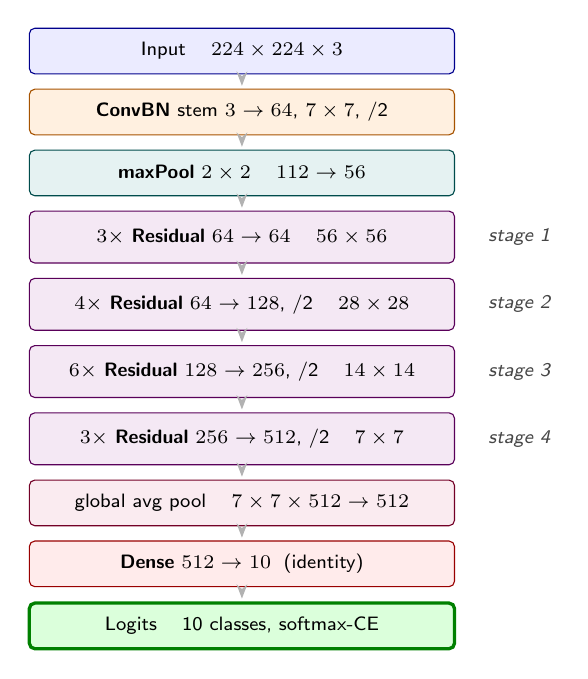
\begin{tikzpicture}[
  >={Stealth[length=1.8mm]},
  every node/.style={font=\sffamily\scriptsize},
  col/.style    = {align=center, rounded corners=2pt, inner sep=2pt, minimum height=0.58cm, minimum width=5.4cm},
  io/.style     = {col, draw=blue!55!black,   fill=blue!8},
  convbn/.style = {col, draw=orange!65!black, fill=orange!12},
  pool/.style   = {col, draw=teal!60!black,   fill=teal!10},
  resid/.style  = {col, draw=violet!70!black, fill=violet!9, minimum height=0.66cm},
  gap/.style    = {col, draw=purple!60!black, fill=purple!8},
  head/.style   = {col, draw=red!60!black,    fill=red!8},
  logits/.style = {col, draw=green!50!black,  fill=green!14, very thick},
  arr/.style    = {->, thick, gray!60, shorten >=1pt, shorten <=1pt},
  stage/.style  = {font=\sffamily\scriptsize\itshape, gray!55!black, anchor=west},
]
  \node[io]                            (input) {Input \;\; $224\times224\times3$};
  \node[convbn, below=0.18cm of input] (stem) {\textbf{ConvBN} stem $3\to64$, $7\times7$, /2};
  \node[pool,   below=0.18cm of stem]  (mp)   {\textbf{maxPool} $2\times2$ \;\; $112\to56$};
  \node[resid,  below=0.18cm of mp]    (s1)   {$3\times$ \textbf{Residual} $64\to64$ \;\; $56\times56$};
  \node[resid,  below=0.18cm of s1]    (s2)   {$4\times$ \textbf{Residual} $64\to128$, /2 \;\; $28\times28$};
  \node[resid,  below=0.18cm of s2]    (s3)   {$6\times$ \textbf{Residual} $128\to256$, /2 \;\; $14\times14$};
  \node[resid,  below=0.18cm of s3]    (s4)   {$3\times$ \textbf{Residual} $256\to512$, /2 \;\; $7\times7$};
  \node[gap,    below=0.18cm of s4]    (g)    {global avg pool \;\; $7\times7\times512 \to 512$};
  \node[head,   below=0.18cm of g]     (d)    {\textbf{Dense} $512\to10$ \;(identity)};
  \node[logits, below=0.18cm of d]     (out)  {Logits \;\; 10 classes, softmax-CE};
  \foreach \a/\b in {input/stem, stem/mp, mp/s1, s1/s2, s2/s3, s3/s4, s4/g, g/d, d/out}
     \draw[arr] (\a) -- (\b);
  \node[stage] at ($(s1.east) + (0.30,0)$) {stage 1};
  \node[stage] at ($(s2.east) + (0.30,0)$) {stage 2};
  \node[stage] at ($(s3.east) + (0.30,0)$) {stage 3};
  \node[stage] at ($(s4.east) + (0.30,0)$) {stage 4};
\end{tikzpicture}

\vspace{0.45cm}

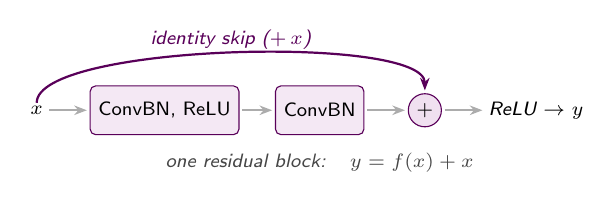
\begin{tikzpicture}[
  >={Stealth[length=1.6mm]},
  every node/.style={font=\sffamily\scriptsize},
  box/.style  = {align=center, rounded corners=2pt, inner sep=3pt, minimum height=0.62cm, draw=violet!70!black, fill=violet!9},
  dot/.style  = {circle, draw=violet!70!black, fill=violet!12, inner sep=0pt, minimum size=0.42cm},
  term/.style = {font=\sffamily\scriptsize\itshape, inner sep=1pt},
  arr/.style  = {->, thick, gray!65, shorten >=1pt, shorten <=1pt},
  skip/.style = {->, thick, violet!70!black, shorten >=1pt},
]
  \node[term]                       (x)   {$x$};
  \node[box, right=0.55cm of x]     (f1)  {ConvBN, ReLU};
  \node[box, right=0.45cm of f1]    (f2)  {ConvBN};
  \node[dot, right=0.55cm of f2]    (sum) {$+$};
  \node[term, right=0.55cm of sum]  (y)   {ReLU $\to y$};
  \draw[arr] (x)  -- (f1);
  \draw[arr] (f1) -- (f2);
  \draw[arr] (f2) -- (sum);
  \draw[arr] (sum) -- (y);
  \draw[skip] (x.north) .. controls +(0,0.75) and +(0,0.75) .. (sum.north)
        node[midway, above, term, violet!70!black] {identity skip ($+\,x$)};
  \node[term, below=0.18cm of f2, gray!55!black] {one residual block: \; $y = f(x) + x$};
\end{tikzpicture}
\end{center}

\subsection*{The verified trainer, which is the pattern every later chapter reuses}
\label{sec:verified_trainer_pattern}

This is the reference configuration. Chapters~\ref{chap:depthwise}
through~\ref{chap:attention} each swap the \texttt{layers} list and change
almost nothing else, so it is worth reading once here rather than four more
times later.

\begin{verbatim}
import LeanMlir

-- 1. The network. A VerifiedNetSpec, not a NetSpec: `slug` names the
--    committed render, and `bnChannels` drives BN statistic threading.
def resnet34Verified : VerifiedNetSpec where
  name     := "ResNet-34"
  slug     := "resnet34"
  inC      := 3
  imageH   := 224
  imageW   := 224
  nClasses := 10
  data     := .imagenette
  layers   := [
    .convBnNB 3 64 7 2,          -- 7x7-s2 stem, no conv bias   224->112
    .maxPool 3 2,                -- He et al. 3x3-s2 OVERLAPPING 112->56
    .residualStage  64  64 3 1,  -- stage 1, 3 blocks            @56
    .residualStage  64 128 4 2,  -- stage 2, downsample + 3      56->28
    .residualStage 128 256 6 2,  -- stage 3, downsample + 5      28->14
    .residualStage 256 512 3 2,  -- stage 4, downsample + 2      14->7
    .globalAvgPool,              -- replaces flatten + fat dense
    .dense 512 10 ]
  bnChannels := #[64, 64,64, ... ]   -- all 36, in forward order

-- 2. The schedule. Everything the optimizer needs beyond the render.
def resnet34Config : VerifiedConfig where
  epochs    := 80
  batchSize := 32

-- 3. The entry point: AdamW, cosine with a 3-epoch warmup, baseLR 1e-3.
def main (argv : List String) : IO Unit :=
  resnet34Verified.toNet.trainAdamSched
    resnet34Config (argv.head?.getD "data") 0.001 0.9 0.999 3 "adam"
\end{verbatim}

\noindent Four things in that listing carry weight, and they are the four to
copy.

\textbf{\texttt{slug} names the artifact.} \texttt{resnet34} resolves to
\texttt{verified\_mlir/resnet34\_adam\_train\_step.mlir}, which is
\texttt{pretty(provenGraph)}: the text the printer emits from the graph the
theorems are about. The trainer does not build a network from this spec at run
time. It loads that file. The spec's job is to say which file, and to be
\texttt{\#guard}ed against it so the two cannot drift.

\textbf{\texttt{bnChannels} is not decoration.} It lists every BatchNorm's
channel count in forward order, and it is what makes
\texttt{trainAdamSched} thread running statistics out of the train step and
into a \emph{separate} evaluation forward. A net that declares BN layers and
then trains through a driver without that threading evaluates against
statistics nobody computed, and reports chance forever. That is a real failure
mode, not a hypothetical, and \S\ref{sec:r34_runit}'s third compile line is
where you can see the machinery that avoids it.

\textbf{\texttt{trainAdamSched}, not \texttt{.train}.} The generic driver is
where the optimizer schedule, the augmentation pipeline and the BN threading
live. \texttt{.train} is the simpler peer from the MNIST chapters and it has
none of the last one.

\textbf{The recipe is arguments, not architecture.} The learning rate, the
momentum pair, the warmup length and the variant string are all passed in.
Swapping AdamW for momentum is a different \emph{argument} against the same
proven gradient, which is exactly what Chapter~\ref{chap:bn} used to measure
optimizers against each other.

\medskip\noindent\textbf{What \texttt{.residualStage} expands to.} It is a
constructor, not a magic word, and the whole of it is twelve lines in
\texttt{LeanMlir/VerifiedSpec.lean}. Every layer reports the parameter
tensors it contributes as \texttt{(dims, initKind)} pairs, where
\texttt{0} is He(fan-in), \texttt{1} is ones ($\gamma$) and \texttt{2} is
zeros ($\beta$ and biases):

\begin{verbatim}
/-- identity basic block @ `c`: two conv->BN->relu units, no projection. -/
private def idBlk (c : Nat) : Array (Array Nat × Nat) :=
  #[(#[c,c,3,3],0),(#[c],1),(#[c],2), (#[c,c,3,3],0),(#[c],1),(#[c],2)]

/-- downsampling basic block `cin->c`: two conv->BN->relu + the 1x1
    option-B projection shortcut (He et al. §3.3). -/
private def downBlk (cin c : Nat) : Array (Array Nat × Nat) :=
  #[(#[c,cin,3,3],0),(#[c],1),(#[c],2), (#[c,c,3,3],0),(#[c],1),(#[c],2),
    (#[c,cin,1,1],0),(#[c],1),(#[c],2)]

private def stageSpec (ic oc count stride : Nat)
    : Array (Array Nat × Nat) := Id.run do
  let mut a := if stride != 1 || ic != oc then downBlk ic oc else idBlk oc
  for _ in [0:count-1] do a := a ++ idBlk oc
  return a

def toSpecs : VLayer -> Array (Array Nat × Nat)
  | dense ic oc             => #[(#[ic,oc],0),(#[oc],2)]      -- Ch. 1
  | relu                    => #[]                            -- Ch. 2
  | conv ic oc k _          => #[(#[oc,ic,k,k],0),(#[oc],2)]  -- Ch. 3
  | maxPool _ _             => #[]                            -- Ch. 3
  | flatten                 => #[]                            -- Ch. 3
  | bnPerChannel oc         => #[(#[oc],1),(#[oc],2)]         -- Ch. 4
  | residualStage ic oc n s => stageSpec ic oc n s            -- here
  | globalAvgPool           => #[]                            -- here
  | bottleneckStage i o n s => bottleneckStageSpec i o n s    -- R50, below
  | ...                        -- 12 more, one per later chapter's block
\end{verbatim}

\noindent Read it against the spec above. \texttt{.residualStage 64 128 4 2}
carries \texttt{stride = 2}, so the condition fires: the first block is a
\texttt{downBlk} --- two $3\times3$ convs plus the $1\times1$ projection that
lets the skip cross a channel change --- and the other three are
\texttt{idBlk}s. Nine tensors plus three sixes, twenty-seven in the stage.
\texttt{.residualStage 64 64 3 1} has \texttt{stride = 1} and
\texttt{ic = oc}, so the condition is false, no projection is emitted, and
all three blocks are identity: eighteen tensors. That one-line conditional is
the entire difference between a stage that changes shape and one that does
not, and it is the same dispatch \texttt{.bottleneckStage} uses for
ResNet-50.

\medskip\noindent It also lets you check the spec against itself. Counting
BatchNorms out of those twelve lines --- one for the stem, then
$3 \times 2$, $3 + 3 \times 2$, $3 + 5 \times 2$ and $3 + 2 \times 2$ for
the four stages --- gives $1 + 6 + 9 + 13 + 7 = 36$, which is exactly the
length \texttt{bnChannels} declares and the thirty-six BatchNorms
\S\ref{sec:residual_r34_example} says the graph computes. Nothing in the
listing is asserted twice; the second number is derived from the first.

\medskip\noindent This is the first chapter that uses the full production recipe (Adam + cosine
+ warmup + weight decay + augmentation + label smoothing) rather
than the s4tfBaseline. Also the first chapter where
\texttt{.globalAvgPool} replaces the flatten-plus-fat-dense head.
\emph{Global average pooling} (GAP) collapses each
\(C \times H \times W\) feature map to a length-\(C\) vector by
averaging over the spatial dimensions,
\[
  \mathrm{gap}(x)_c \;=\; \frac{1}{HW} \sum_{i, j} x_{c, i, j},
\]
so the classifier head sees one summary scalar per channel instead
of the full \(C \cdot H \cdot W\) flattened activation. That's the
architectural move that drops ResNet-34 from what would have been a
$\sim$200M parameter AlexNet-era spec down to 21.3M. We'll see GAP
again as the ``Squeeze'' step inside the squeeze-and-excitation
block in Chapter~\ref{chap:se}, and at the head of every
post-2015 vision architecture in the bestiary.

\subsection*{Results}

\S\ref{sec:r34_runit} has the run: 80 epochs at about 65 seconds each on one
RTX 4060 Ti, roughly an hour and a half, finishing at \textbf{89.71\%} top-1
and \textbf{98.27\%} top-5 on Imagenette's 3,925-image validation split. That
is the going rate for a scratch-trained ResNet-34 at this resolution and data
size. Rather than reprint the log, here is what is worth noticing in it.

- \textbf{21.3M parameters, and 729\,KB of MLIR} (728\,801 chars) for the
  entire AdamW training step. That is $112\times$ the MNIST MLP's render and
  only $6\times$ the wide CIFAR BatchNorm net's, against a network that is far
  more than six times the earlier one. Emission is per-op, not per-parameter,
  so $3 \times 3$ convolutions at 64 and at 512 channels cost the same handful
  of lines. Depth grows the text linearly, and width does not grow it at all.

- \textbf{Per-step time is about 220\,ms} at batch 32, 295 steps to the epoch,
  dominated by the four \texttt{.residualStage} groups where the $3 \times 3$
  convolutions at 64, 128, 256 and 512 channels are. The first stage alone at
  64 channels does $3 \times 3 \times 64 \times 64$ multiply-accumulates per
  output spatial location, about $3.4 \times 10^8$ FLOPs per forward image,
  times the batch, times three blocks at that width, times two for the
  backward.

- \textbf{Three artifacts, not one.} The train step is accompanied by
  \texttt{resnet34\_fwd} (98\,383 chars) and
  \texttt{resnet34\_fwd\_eval} (76\,720 chars). The last exists only because
  BatchNorm evaluates differently than it trains, and it is the concrete cost
  of the \texttt{bnChannels} line in the spec above.

- \textbf{Final loss plateaus near 0.50}, not zero. That's the
  label-smoothing floor: with $\epsilon = 0.1$ and 10 classes, the
  minimum possible cross-entropy against a smoothed target is
  $-0.9 \log 0.9 - 0.1 \log (0.1/9) \approx 0.485$. The 0.50 value
  at epoch 80 means the model has essentially converged. More
  epochs would mostly just extend training time without budging the
  loss.

- \textbf{BN layers: 36}. Every residual block contains two normalized
  convolutions, and there are 16 residual blocks across the four stages
  (3+4+6+3). Plus the stem. That is 33 from the
  \texttt{.residualStage} expansions plus 3 stem and projection layers,
  for 36 total. Each one proves its own VJP via
  \S~\ref{thm:bn_has_vjp} and composes with the rest of the network
  via \S~\ref{thm:vjp_comp}.

\section{MLIR: Residual}

\noindent\textbf{What is already proven.} A residual block is
$\mathrm{residual}(x) = f(x) + x$, an additive fan-in, where $f$ is the
conv\,$\to$\,BN\,$\to$\,relu\,$\to$\,conv\,$\to$\,BN inner block. As
Theorem~\ref{thm:residual_has_vjp} states, its reverse-mode derivative is
the additive-fan-in rule with the identity in one slot: \emph{send the
upstream gradient through both branches and add}.
\texttt{residual\_has\_vjp\_at} proves exactly this at the evaluation point
(a one-line proof: the fan-in lemma with the identity's VJP plugged into
one slot), and the inner $f$'s VJP is the convolution and BatchNorm
backward already proven in Chapters~\ref{chap:cnn} and~\ref{chap:bn}. The
whole block, and a tower of sixteen of them, composes by the chain
rule \texttt{vjp\_comp\_at} (\S~\ref{thm:vjp_comp}).

\medskip\noindent\textbf{The gap and how we close it.} The residual
fan-in is the structural heart of a deep ResNet. The emitted backward is
given a denotation valued in the proofs' own tensor type, shown equal to
\texttt{residual\_has\_vjp\_at}'s backward, and the structural move is
visible in the emitted text. The forward
saves $\texttt{add} = f(x) + x$ and the block output
$\texttt{relu}(\texttt{add})$. The backward first pushes the incoming
cotangent back through that relu (a \texttt{compare}/\texttt{select} at the
post-add, giving \texttt{\%dadd}), and then, and this is the fan-in, sends
\texttt{\%dadd} through \emph{both} branches and adds (the inner block's
forward and $f$-backward elided, as they are the conv/BN nodes of
Chapters~\ref{chap:cnn}--\ref{chap:bn}):

\begin{verbatim}
// forward (saved): %out = f(%x)  [conv-BN-relu-conv-BN, Ch. 4-5]
//                  %add = %out + %x
%madd = stablehlo.compare GT, %add, %zc
          : (tensor<1x2x4x4xf32>, tensor<1x2x4x4xf32>)
            -> tensor<1x2x4x4xi1>
%dadd = stablehlo.select %madd, %dOut, %zc
          : tensor<1x2x4x4xi1>, tensor<1x2x4x4xf32>
// %dF = f.backward(%dadd)  [conv/BN/relu input-VJP chain, Ch. 4-5]
%dx = stablehlo.add %dF, %dadd : tensor<1x2x4x4xf32>
return %dx : tensor<1x2x4x4xf32>
\end{verbatim}

\noindent Read it against the theorem: \texttt{\%dadd} is the cotangent at
the fan-in, and it appears \emph{twice} in the last two lines, once as
the input to $f$'s backward (\texttt{\%dF}, the gradient through the
residual function) and once added directly (\texttt{\%dx = \%dF + \%dadd},
the gradient straight down the identity skip). That single
\texttt{stablehlo.add} \emph{is} ``send the gradient through both branches
and add'': the skip term is the same \texttt{\%dadd} the block term started
from, which is why the gradient survives all sixteen blocks instead of
attenuating away. The inner $f$ backward that computes \texttt{\%dF}, the
convolution and BatchNorm input-VJPs, is bridged op by op exactly as in
Chapters~\ref{chap:cnn} and~\ref{chap:bn}. Only the fan-in is new here.

\medskip\noindent\textbf{Caveats.}
\begin{itemize}
  \item \textbf{The fan-in \texttt{add} is unconditional}, because addition is
    linear, so that bridge holds at every input.
  \item \textbf{The post-add ReLU is a smooth-point bridge} (no
    pre-activation exactly zero), and the two BatchNorms inside $f$ carry
    their own $\epsilon > 0$ conditions from Chapter~\ref{chap:bn}.
  \item \textbf{Representative scale}, a two-channel block at $4\times4$. The
    same \texttt{\%dadd} fan-in repeats for all sixteen blocks.
\end{itemize}

\section{What's in the production recipe?}
\label{sec:r34_recipe}

Six ingredients first appear here, none of which are layers. They
all live in \texttt{TrainConfig} or training code. They don't touch
the network, but they're what moves a scratch-trained model from 72.82\%
(plain SGD + momentum, no other tricks) to 90.29\%.

\textbf{Adam} (Kingma \& Ba, 2014,
\href{https://arxiv.org/abs/1412.6980}{arXiv:1412.6980}). Replaces
vanilla SGD. Maintains
per-parameter running estimates of the first and second moments of
the gradient and uses them for an adaptive per-parameter learning
rate. Much faster convergence than SGD on most tasks, much more
forgiving of learning-rate choice.

\textbf{Cosine learning-rate schedule} (Loshchilov \& Hutter, 2016,
\href{https://arxiv.org/abs/1608.03983}{arXiv:1608.03983}).
After warmup, the learning rate decays from its peak to near-zero
following $\mathrm{lr}(t) = \mathrm{lr}_{\max} \cdot \tfrac{1}{2}(1 +
\cos(\pi t / T))$. Smoother than step schedules, and consistently produces
slightly better final losses in practice. Paired with warmup and
\href{https://www.fast.ai/posts/2018-04-30-dawnbench-fastai.html}{progressive
resizing} (Howard et al., 2018), this was the winning recipe at
Stanford's DAWNBench in 2018. The lineage traces back to Leslie
Smith's cyclical learning rates (Smith 2015,
\href{https://arxiv.org/abs/1506.01186}{arXiv:1506.01186}).
Popularized for ImageNet-scale training by He et al.\ 2018's
``Bag of Tricks''
(\href{https://arxiv.org/abs/1812.01187}{arXiv:1812.01187}).

\textbf{Warmup} (Goyal et al., 2017,
\href{https://arxiv.org/abs/1706.02677}{arXiv:1706.02677}). Linearly
ramps the learning rate from zero to its
peak over the first few epochs (3 for ResNet-34). Stabilizes early
training when gradients are still reorganizing randomly-initialized
weights. Becomes essential for larger models and larger batches, and by
ViT-Tiny in Chapter~\ref{chap:attention} it's a necessity.

\textbf{Weight decay}. Adds a small L2 shrink to all trainable weights
each step: $w \leftarrow w - \eta \lambda w$. Regularizer, discourages
weights from growing without bound. Loshchilov \& Hutter's
``decoupled'' variant (\textbf{AdamW}, 2017,
\href{https://arxiv.org/abs/1711.05101}{arXiv:1711.05101}) is what
actually ships in modern
pipelines, and it's what \texttt{TrainConfig.weightDecay} implements.

\textbf{Augmentation}. Our pipeline does random crops ($256 \to 224$)
and random horizontal flips on Imagenette, hflip only on CIFAR, and
nothing on MNIST. Lives in the data pipeline, not the network. We
will explore data augmentation strategies in upcoming chapters.

\textbf{Label smoothing} (Szegedy et al., 2016,
\href{https://arxiv.org/abs/1512.00567}{arXiv:1512.00567}). Replaces
the one-hot
target with a smoothed $(\varepsilon / (K-1), \ldots, 1 - \varepsilon,
\ldots)$. Stops the network from producing arbitrarily large logits on
the correct class, which keeps training stable and improves calibration.
Explains the \textbf{0.50 loss floor} in the Results section above:
$-0.9 \log 0.9 - 0.1 \log (0.1/9) \approx 0.485$.

Every chapter after this one uses the same six ingredients. The
\texttt{NetSpec} changes, and the recipe stays.

\section{Ablation: what each ingredient contributes}
\label{sec:r34_ablation}

So how much does each ingredient actually earn? We ran the full
recipe plus six leave-one-out variants on ResNet-34 Imagenette, 80
epochs each, same init and batch order. Each ablation row keeps
everything except the one named component, so the lift measures
that component's contribution given everything else is present. It is
an honest answer to ``is this piece pulling its weight?'' rather
than the order-dependent story you'd get from an additive ladder.

\begin{center}
\begin{tabular}{l r r}
\hline
Run & Val accuracy & $\Delta$ vs full \\
\hline
Full recipe             & 90.29\% & --- \\
Bare recipe (plain SGD + momentum, no other tricks) & 72.82\% & $-$17.47 \\
Full minus basic augmentation & 82.71\% & $-$7.58 \\
Full minus cosine decay & 86.81\% & $-$3.48 \\
Full minus Adam (vanilla SGD, lr 0.01) & 87.04\% & $-$3.25 \\
Full minus warmup       & 88.88\% & $-$1.41 \\
Full minus label smoothing & 89.24\% & $-$1.05 \\
Full minus weight decay & 89.68\% & $-$0.61 \\
\hline
\end{tabular}
\end{center}

Three observations worth naming:

\textbf{Augmentation is by far the largest single contribution}
($-$7.58 points, more than 2$\times$ any other knob). Imagenette
has just 9469 training images for a 21M-parameter network, so
without augmentation the model overfits hard, and training loss
drops below $0.001$ while val accuracy stalls. Augmentation is
doing most of the work that the rest of the recipe gets credit
for.

\textbf{Cosine decay and Adam are roughly tied for largest
non-augmentation contribution} ($-$3.48 and $-$3.25 points). They
operate on different axes, with cosine shaping the learning-rate
trajectory and Adam the per-parameter update magnitude, but
their late-training influence on val accuracy is comparable.

\textbf{The contributions are essentially additive.} Sum of all
six leave-one-out deltas: $-17.38$ points. Bare-recipe delta vs
full: $-17.47$ points. The two agree to within rounding, suggesting
the modern recipe's ingredients aren't significantly interacting.
Each one buys roughly the same lift independently of which others
are present. Weight decay and label smoothing are the smallest
contributors ($-$0.61 and $-$1.05) but show the
overfit-then-catch-up signature mid-training (e.g., no-WD lands
$-$6 points at epoch 10 before the gap narrows by epoch 80).

A note on the SGD configs: \texttt{r34-no-adam} replaces Adam with
vanilla SGD at lr=0.01 (no momentum), keeping everything else from
the full recipe. \texttt{r34-bare} uses SGD with momentum 0.9 at
lr=0.01 and turns \emph{all} other tricks off. The two SGD configs
therefore differ on momentum as well as on the recipe ingredients,
so the bare row should be read as a ``what does the modern recipe
buy us total'' baseline rather than a strict additive component of
the leave-one-out chain.

\section{ImageNet recipe}

The Imagenette runs above all trained on $\sim$9.5K images for 80
epochs. This section is the same 21.8M-parameter network on 1.28M images
and 1000 classes, trained on the paper's 90-epoch schedule. The
architecture is unchanged. Only the dataset, the output head width, and
the training schedule differ.

Ninety epochs at global batch 256 is what He et al.\ ran, and this section
runs it \emph{twice}: once on the verified codegen path and once on the JAX
reference. Both paths share everything above the data loader --- the
architecture, the \texttt{.train} invocation, and every recipe knob --- so
the only thing that differs is how the graph reaches the GPU.

The recipe in full: SGD with momentum $0.9$ at batch 256, cosine LR with a
5-epoch warmup from peak $0.1$, label smoothing $0.1$, Inception-style
random-resized-crop (sampling $8$--$100\%$ of the image area at a
$\frac{3}{4}$--$\frac{4}{3}$ aspect ratio, then resizing to
$224\times224$) plus a horizontal flip, and $\ell_2$ weight decay
$10^{-4}$. Every one of those is either the original paper or the ``bag of
tricks'' polish that became standard after it, and
\S\ref{sec:r50_a3_vs_2018} is the table that says which is which.

\prosesection{The PJRT lowerer}
\label{sec:r34_phase4}

The verified path is a second trusted lowerer, \texttt{ffi/pjrt\_ffi.c}: it
implements the same C surface as the IREE shim and hands the graph to XLA
through the PJRT C API. Nothing above the shim changes. The
backend is whichever \texttt{.so} the binary linked, and backend
detection is a weak symbol, so a binary cannot disagree with the library
it linked. There is no Python at run time. What the trainer
executes is \texttt{pretty(provenGraph)}: the same rendered artifact the
proofs reason about, not a hand-written emitter.

Here is the trainer:

\begin{verbatim}
-- 1. Same backbone as the Imagenette net, 1000 classes instead of 10.
def resnet34ImagenetVerified : VerifiedNetSpec where
  name     := "ResNet-34 (ImageNet-1k)"
  slug     := "resnet34in"
  inC      := 3
  imageH   := 224
  imageW   := 224
  nClasses := 1000
  data     := .imagenet
  shimScript := "generated_resnet34_imagenet_shim.py"
  layers   := [
    .convBnNB 3 64 7 2,          -- 7x7-s2 stem -> BN -> relu    224->112
    .maxPool 3 2,                -- He et al. 3x3-s2, OVERLAPPING 112->56
    .residualStage  64  64 3 1,  -- stage1: 3 identity            @56
    .residualStage  64 128 4 2,  -- stage2: downsample + 3        56->28
    .residualStage 128 256 6 2,  -- stage3: downsample + 5        28->14
    .residualStage 256 512 3 2,  -- stage4: downsample + 2        14->7
    .globalAvgPool,
    .dense 512 1000 ]
  bnChannels := #[64, 64,64, 64,64, ... ]   -- all 36, in forward order

-- The head is the ONLY thing that may differ from the 10-class net.
-- Anything else moving means the spec drifted from its Imagenette twin.
#guard resnet34ImagenetVerified.toSpecs.size == resnet34Verified.toSpecs.size
#guard resnet34ImagenetVerified.toSpecs.pop.pop == resnet34Verified.toSpecs.pop.pop
#guard resnet34ImagenetVerified.toSpecs.back!  == (#[1000], 2)

-- 2. 90 epochs at batch 256 — the paper schedule.
def resnet34ImagenetConfig : VerifiedConfig where
  epochs    := 90
  batchSize := 256

-- 3. The entry point. Heavy-ball momentum, cosine with a 5-epoch warmup
--    at peak 0.1, weight decay 1e-4, label smoothing 0.1.
def main (argv : List String) : IO Unit :=
  resnet34ImagenetVerified.toNet.trainAdamSched
    resnet34ImagenetConfig (argv.head?.getD "data") 0.1 0.9 0.999 5 "mom256"
\end{verbatim}

\noindent That is \texttt{apps/imagenette/MainResnet34Imagenet.lean}, built as
\texttt{lake build resnet34-imagenet-verified}, and it is the program the
numbers below came from. Three things in it are worth
pulling out, because they are what makes the listing a claim rather than a
description.

\textbf{The \texttt{slug} is the artifact.} \texttt{resnet34in} names
\texttt{verified\_mlir/resnet34in\_mom256\_train\_step.mlir}, which is
\texttt{pretty(provenGraph)} off the same renderer every earlier chapter used.
Scaling to ImageNet needed nothing new in it. \texttt{nClasses}, the batch, the
optimizer and the slug are all ordinary parameters, so the ImageNet artifacts
are three \texttt{\#eval}s of machinery that was already proved. What had to be
built was the data path, not the compiler.

\textbf{The \texttt{\#guard}s pin it to the Imagenette net.} The 1000-class
spec must be the 10-class one with a different head, and the three guards fail
the build if any other parameter shape moves. That is what licenses reading the
Imagenette chapter's theorems as being about this network's body.

\textbf{The \texttt{shimScript} is per-net and load-bearing.} It names this
net's own generated augmentation shim. Every net used to stream ResNet-34's,
which meant an augmentation mismatch could hide inside a fair-looking
comparison. Here it is the same shim the JAX reference consumes, which is what
makes the two a matched pair rather than two separate stories.


\medskip\noindent It runs with:

\begin{verbatim}
CUDA_VISIBLE_DEVICES=0,2,3,4 PJRT_REPLICAS=4 LEAN_MLIR_REPLICAS=4 \
  SHIM_WORKERS=8 PJRT_FFI_RESIDENT=1 \
  LEAN_MLIR_VARIANT=momdp64 LEAN_MLIR_BATCH=64 \
  .lake/build/bin/resnet34-imagenet-verified data
\end{verbatim}

\begin{center}
\begin{tabular}{l l r r r r r}
\hline
GPU & Precision & Per epoch & Epochs & Total & Val top-1 & Val top-5 \\
\hline
4$\times$ 4060 Ti (CUDA)  & fp32 & $\sim$24.7 min & 90 & $\sim$37.1 hr & $\mathbf{74.14\%}$ & $\mathbf{91.86\%}$ \\
2$\times$ 7900 XTX (ROCm) & fp32 & ---            & 90 & ---           & --- & --- \\
\hline
\end{tabular}
\end{center}

\noindent Global batch 256 as $4 \times 64$ replicas, fp32 throughout. The
ROCm row is a \texttt{[TODO]}: the same render, the same C surface, a
different backend \texttt{.so}.

\begin{center}
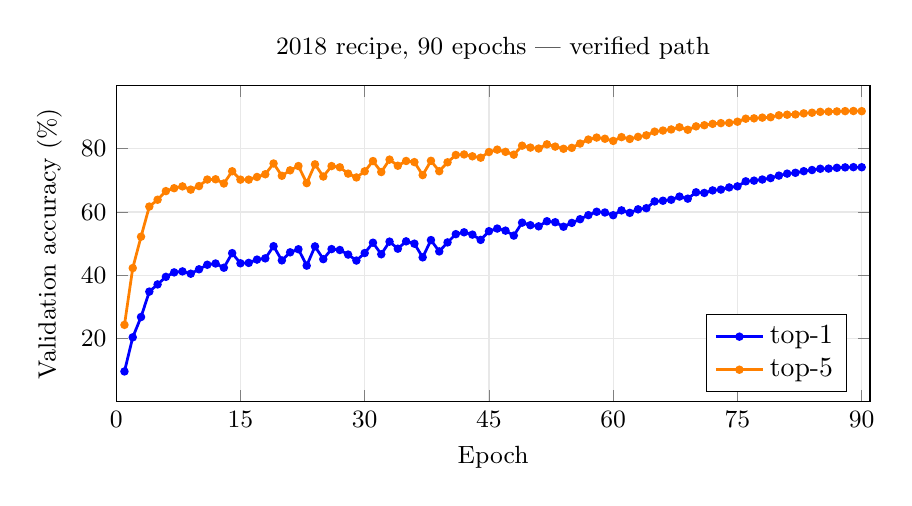
\begin{tikzpicture}
\begin{axis}[
    width=0.92\linewidth, height=5.6cm,
    xlabel={Epoch}, ylabel={Validation accuracy (\%)},
    xmin=0, xmax=91, ymin=0, ymax=100,
    xtick={0,15,30,45,60,75,90},
    ytick={20,40,60,80},
    legend pos=south east,
    legend cell align={left},
    grid=major, grid style={gray!18},
    tick label style={font=\small},
    label style={font=\small},
    title style={font=\small},
    every axis plot/.append style={line width=1pt, mark size=1pt},
    title={2018 recipe, 90 epochs --- verified path},
]
\addplot[blue, mark=*, mark options={fill=blue}] coordinates {
(1,9.60) (2,20.39) (3,26.81) (4,34.83) (5,37.11) (6,39.50) (7,40.91) (8,41.22) (9,40.49) (10,41.89) (11,43.32) (12,43.72) (13,42.38) (14,46.99) (15,43.78) (16,43.91) (17,44.95) (18,45.34) (19,49.18) (20,44.70) (21,47.25) (22,48.22) (23,43.04) (24,49.12) (25,45.10) (26,48.27) (27,47.98) (28,46.54) (29,44.65) (30,47.02) (31,50.28) (32,46.64) (33,50.63) (34,48.39) (35,50.72) (36,49.98) (37,45.66) (38,51.12) (39,47.54) (40,50.38) (41,52.99) (42,53.58) (43,52.84) (44,51.18) (45,53.92) (46,54.76) (47,54.10) (48,52.54) (49,56.62) (50,55.83) (51,55.47) (52,57.07) (53,56.76) (54,55.34) (55,56.55) (56,57.72) (57,59.00) (58,60.07) (59,59.84) (60,58.98) (61,60.51) (62,59.72) (63,60.84) (64,61.19) (65,63.33) (66,63.55) (67,63.86) (68,64.87) (69,64.21) (70,66.22) (71,66.02) (72,66.82) (73,67.09) (74,67.76) (75,68.10) (76,69.69) (77,69.90) (78,70.26) (79,70.71) (80,71.49) (81,72.12) (82,72.38) (83,72.89) (84,73.26) (85,73.66) (86,73.71) (87,73.95) (88,74.10) (89,74.17) (90,74.14)
};
\addlegendentry{top-1}
\addplot[orange, mark=*, mark options={fill=orange}] coordinates {
(1,24.32) (2,42.27) (3,52.19) (4,61.72) (5,63.87) (6,66.60) (7,67.51) (8,68.09) (9,67.06) (10,68.19) (11,70.25) (12,70.34) (13,69.00) (14,72.87) (15,70.22) (16,70.22) (17,71.06) (18,71.92) (19,75.32) (20,71.44) (21,73.17) (22,74.52) (23,69.12) (24,75.06) (25,71.21) (26,74.51) (27,74.13) (28,72.12) (29,70.91) (30,72.85) (31,76.09) (32,72.63) (33,76.55) (34,74.61) (35,76.12) (36,75.76) (37,71.66) (38,76.17) (39,72.89) (40,75.70) (41,78.01) (42,78.18) (43,77.60) (44,77.15) (45,78.95) (46,79.70) (47,79.01) (48,78.11) (49,80.95) (50,80.36) (51,80.05) (52,81.38) (53,80.66) (54,79.97) (55,80.27) (56,81.63) (57,82.89) (58,83.52) (59,83.14) (60,82.46) (61,83.66) (62,83.08) (63,83.74) (64,84.23) (65,85.39) (66,85.74) (67,86.08) (68,86.78) (69,85.98) (70,87.06) (71,87.42) (72,87.85) (73,88.08) (74,88.16) (75,88.53) (76,89.48) (77,89.59) (78,89.82) (79,89.95) (80,90.56) (81,90.74) (82,90.82) (83,91.17) (84,91.37) (85,91.64) (86,91.70) (87,91.78) (88,91.87) (89,91.91) (90,91.86)
};
\addlegendentry{top-5}
\end{axis}
\end{tikzpicture}
\end{center}

\noindent The run above, epoch by epoch. One attempt, no thermal rest and no
PCIe interruption across all 90.

\prosesection{The JAX lowerer}

The JAX trainer lives in
\texttt{jax/\allowbreak Main\allowbreak Resnet\allowbreak Imagenet.lean}, builds as
\texttt{lake build resnet34-\allowbreak imagenet}, and wires \texttt{.imagenet}
through tfds streaming. It runs the same recipe on the same cards, and its job
here is to be the independent second implementation the verified number is
checked against.

It runs in bf16: the spec casts both matmuls and convolutions to bfloat16
while keeping fp32 master weights. NVIDIA's tensor cores run bf16 convolution
about $1.6\times$ faster than fp32 --- the opposite of AMD's MIOpen, where it is
a wash, which is why conv precision sits behind its own \texttt{bf16Conv} flag.
That is the whole reason the reference column below is roughly three times
quicker than the verified one: a throughput choice, not a fidelity one.

\begin{center}
\begin{tabular}{l l r r r r r}
\hline
GPU & Precision & Per epoch & Epochs & Total & Val top-1 & Val top-5 \\
\hline
4$\times$ 4060 Ti (CUDA)  & fp32 & $\sim$16.8 min & 90 & $\sim$25 hr & --- & --- \\
4$\times$ 4060 Ti (CUDA)  & bf16 & $\sim$8.8 min  & 90 & $\sim$14.8 hr & $\mathbf{74.16\%}$ & $\mathbf{91.92\%}$ \\
1$\times$ A100 (CUDA)     & bf16 & ---            & 90 & $\sim$9 hr & --- & --- \\
1$\times$ MI300X (ROCm)\textsuperscript{\dag}   & bf16 & $\sim$3.5 min & 90 & $\sim$5.4 hr & \withheld & \withheld \\
\hline
\end{tabular}
\end{center}

\noindent Per-epoch throughput for the same recipe on other hardware. The
A100 row is a wall-clock estimate. \textsuperscript{\dag}\,MI300X ran at batch 1024 / lr 0.4 and before the
current validation protocol, so only its throughput is quotable.

\begin{center}
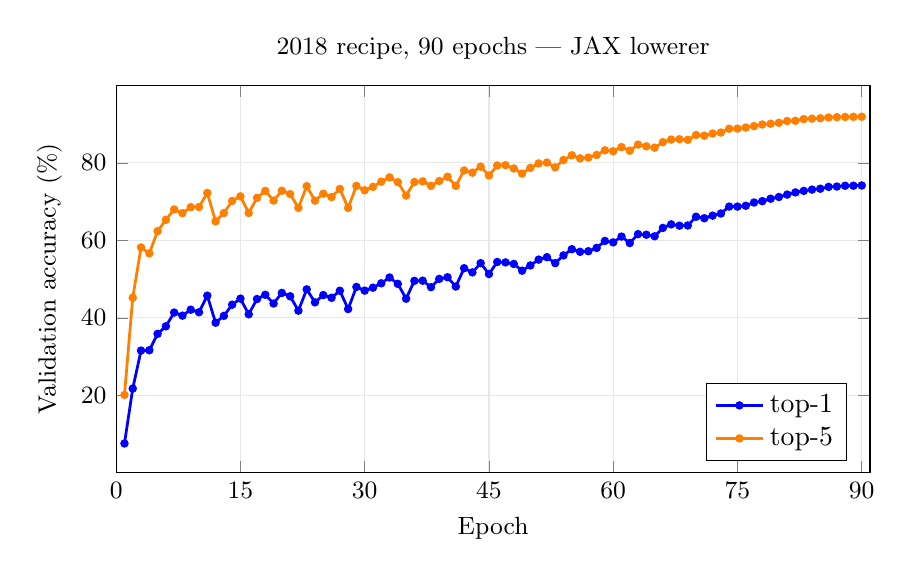
\begin{tikzpicture}
\begin{axis}[
    width=0.92\linewidth, height=6.5cm,
    xlabel={Epoch}, ylabel={Validation accuracy (\%)},
    xmin=0, xmax=91, ymin=0, ymax=100,
    xtick={0,15,30,45,60,75,90},
    ytick={20,40,60,80},
    legend pos=south east,
    legend cell align={left},
    grid=major, grid style={gray!18},
    tick label style={font=\small},
    label style={font=\small},
    every axis plot/.append style={line width=1pt, mark size=1pt},
    title style={font=\small},
    title={2018 recipe, 90 epochs --- JAX lowerer},
]
\addplot[blue, mark=*, mark options={fill=blue}] coordinates {
(1,7.54) (2,21.73) (3,31.53) (4,31.62) (5,35.85) (6,37.80) (7,41.35) (8,40.55) (9,42.09) (10,41.43) (11,45.71) (12,38.73) (13,40.50) (14,43.38) (15,44.94) (16,40.91) (17,44.84) (18,45.94) (19,43.69) (20,46.42) (21,45.55) (22,41.84) (23,47.34) (24,43.98) (25,45.86) (26,45.16) (27,46.98) (28,42.26) (29,47.96) (30,47.01) (31,47.77) (32,48.91) (33,50.40) (34,48.76) (35,44.92) (36,49.54) (37,49.58) (38,47.91) (39,50.04) (40,50.47) (41,48.07) (42,52.80) (43,51.72) (44,54.10) (45,51.30) (46,54.40) (47,54.30) (48,53.90) (49,52.16) (50,53.51) (51,55.02) (52,55.65) (53,54.11) (54,56.11) (55,57.71) (56,57.03) (57,57.19) (58,58.04) (59,59.84) (60,59.47) (61,60.97) (62,59.30) (63,61.60) (64,61.44) (65,61.05) (66,63.21) (67,64.12) (68,63.78) (69,63.83) (70,66.09) (71,65.70) (72,66.37) (73,66.93) (74,68.71) (75,68.71) (76,68.92) (77,69.76) (78,70.11) (79,70.75) (80,71.19) (81,71.81) (82,72.37) (83,72.76) (84,73.10) (85,73.33) (86,73.80) (87,73.89) (88,74.09) (89,74.10) (90,74.16)
};
\addlegendentry{top-1}
\addplot[orange, mark=*, mark options={fill=orange}] coordinates {
(1,20.09) (2,45.19) (3,58.17) (4,56.65) (5,62.37) (6,65.29) (7,67.97) (8,67.02) (9,68.56) (10,68.60) (11,72.23) (12,64.91) (13,67.05) (14,70.17) (15,71.36) (16,67.07) (17,70.97) (18,72.76) (19,70.27) (20,72.81) (21,71.93) (22,68.39) (23,73.98) (24,70.24) (25,72.04) (26,71.17) (27,73.27) (28,68.36) (29,74.05) (30,72.92) (31,73.81) (32,75.14) (33,76.26) (34,75.01) (35,71.57) (36,75.05) (37,75.23) (38,74.08) (39,75.32) (40,76.41) (41,74.06) (42,78.04) (43,77.47) (44,79.03) (45,76.75) (46,79.32) (47,79.42) (48,78.55) (49,77.24) (50,78.71) (51,79.86) (52,80.08) (53,78.84) (54,80.74) (55,81.97) (56,81.16) (57,81.37) (58,82.04) (59,83.24) (60,83.00) (61,84.05) (62,83.15) (63,84.72) (64,84.26) (65,83.93) (66,85.34) (67,86.02) (68,86.11) (69,85.95) (70,87.20) (71,87.02) (72,87.58) (73,87.84) (74,88.82) (75,88.85) (76,89.12) (77,89.49) (78,89.91) (79,90.11) (80,90.35) (81,90.81) (82,90.86) (83,91.30) (84,91.42) (85,91.52) (86,91.72) (87,91.80) (88,91.85) (89,91.89) (90,91.92)
};
\addlegendentry{top-5}
\end{axis}
\end{tikzpicture}
\end{center}

\noindent The same recipe, epoch by epoch, through the JAX lowerer. The kink
near epoch~5 is the end of warmup; the steady late climb is the cosine anneal.

\prosesection{The two paths, side by side}

\begin{center}
\begin{tabular}{@{}l l l@{}}
\hline
 & verified lowerer (PJRT) & JAX lowerer \\
\hline
lowering            & \texttt{pretty(provenGraph)} $\to$ XLA & JAX $\to$ XLA \\
Python at run time  & none                     & yes \\
precision           & fp32                     & bf16 (matmul + conv) \\
BN statistic group  & 64 (per replica)         & 256 (global) \\
per epoch           & $\sim$24.7 min           & $\sim$8.8 min \\
total               & $\sim$37.1 hr            & $\sim$14.8 hr \\
\hline
\textbf{val top-1}  & $\mathbf{74.14\%}$       & $\mathbf{74.16\%}$ \\
\textbf{val top-5}  & $\mathbf{91.86\%}$       & $\mathbf{91.92\%}$ \\
\hline
\end{tabular}
\end{center}

\noindent Both columns are ResNet-34 on the 2018 recipe, 90 epochs, global
batch 256, on the same four 4060\,Ti cards, scored over the same $50{,}000$
validation images under the same protocol. Everything above the rule differs
between them; everything below it does not. A ROCm column
(2$\times$ 7900 XTX) is \withheld{} pending hardware.

\noindent Global batch 256 as $4 \times 64$, heavy-ball momentum with coupled
$\ell_2$, cosine with a 5-epoch warmup at peak $0.1$, weight decay $10^{-4}$,
label smoothing $0.1$ --- the same recipe, knob for knob, on both lowerers. The paper schedule at 90 epochs, completed in $37.1$ hours on one
attempt, with no thermal rest and no PCIe interruption.

\medskip\noindent\textbf{The two paths agree to $0.02$ points.} Same
architecture, same recipe, same box, same $50{,}000$ images under the same
protocol --- but one lowered through JAX and the other through
\texttt{pretty(provenGraph)} into XLA with no Python at run time. It is the
closest verified-versus-reference pair in this book.

\medskip\noindent It is also a harder test than it looks. The JAX trainer
runs under \texttt{@jit} with a \texttt{NamedSharding} mesh, so its BatchNorm
means carry global semantics and XLA reduces them across all four cards: the
statistic group is the whole $256$. This run is four replicas of $64$ with no
collective touching the batch statistics, so its group is $64$ --- a fourfold
difference that moved the answer by two hundredths of a point.

\medskip\noindent The two \emph{lowerers} agree as tightly as the two paths
do. Run from the same initialization on the same box, IREE and PJRT scored
\textbf{17{,}312} and \textbf{17{,}313} correct at epoch~5 --- one image apart.
The proof-carrying tier stops at Imagenette, so the claim is \emph{one
architecture, two independent lowerings, agreeing}, not ``proven at ImageNet
scale''.



\prosesection{A reasonable stopping point}

For the fastest path through this book, the route is roughly:

\begin{itemize}
  \item The intro chapters \& Ch 1: framework setup (mandatory context).
  \item Ch 2--3: MLP and CNN worked examples, the simplest cases
    of the framework reaching real architectures.
  \item Skim Ch~\ref{chap:bn} (BatchNorm). It's structurally the
    hardest chapter and the prose says so up front. The math is
    right (\texttt{pdiv\_bnNormalize}'s three-term cancellation is
    formalized and matches the codegen), but it's not the place to
    spend time if you're not specifically interested in BN. Spend
    time running as many MNIST and CIFAR demos as possible.
  \item Read this chapter (Ch~\ref{chap:residual}, ResNet-34).
    Residual blocks are where the chain rule shows it can carry
    composition through arbitrarily deep architectures, and the proof
    reduces to one additive-fan-in lemma you've already seen. Run
    the ResNet-50 RSB-A3 ImageNet training demo locally and/or in
    the cloud ($\sim$6--9\,hrs, $\sim$\$15 in compute).
  \item Stop here. Assume Chapters \ref{chap:depthwise}--\ref{chap:attention}
    (MobileNet, EfficientNet, ConvNeXt, ViT) and the Bestiary
    (Ch~\ref{chap:bestiary}) are correct, because they all reuse the
    same framework with new operators slotting into the same proof
    tree. Appendix~\ref{app:verification} walks through how that
    claim is auditable if you ever want to spot-check it.
\end{itemize}

Reading through Ch 5 is enough to know the framework works. Read
the AlphaGo Zero paper
(\bestiaryref{bestiary:alphagozero}{bestiary entry}), which combines
reinforcement learning with a large residual network of
convolutions.

\section{ResNet-50 on ImageNet: the 2018 recipe and RSB-A3}

\imagenetphasenote

The basic block ResNet-34 is built from generalizes to the
\emph{bottleneck} block of ResNet-50, and the \texttt{jax/} folder
ships it as a full ImageNet demo
(\texttt{jax/MainResnet50Imagenet.lean}) trained on the modern
``ResNet Strikes Back'' A3 recipe (Wightman et al.\ 2021): LAMB at
effective batch 2048 (via gradient accumulation), BCE over
Mixup/CutMix soft targets, RandAugment, train@160 / eval@224. On the
same proven-backward bottleneck codegen it reached $\mathbf{78.26\%}$
top-1 / $\mathbf{93.79\%}$ top-5 at 100 epochs, clearing the paper's
$78.1\%$ and the $78.05\%$ that \texttt{timm}'s own
\texttt{resnet50.a3\_in1k} weights score under the same protocol.

\prosesection{The JAX lowerer}

\begin{center}
\begin{tabular}{l l l r r r r r}
\hline
GPU & Recipe & BN regime & Per epoch & Ep. & Total & top-1 & top-5 \\
\hline
4$\times$ 4060 Ti (bf16)  & 2018   & global (256)    & $\sim$14.8 min & 90  & $\sim$24.0 hr & $\mathbf{76.95\%}$ & $\mathbf{93.44\%}$ \\
4$\times$ 4060 Ti (bf16)  & RSB-A3 & Ghost-BN (512)  & $\sim$7.9 min & 100 & $\sim$15.1 hr & $\mathbf{78.26\%}$ & $\mathbf{93.79\%}$ \\
\hline
\end{tabular}
\end{center}

\noindent ResNet-50 on the same four 4060\,Ti cards, both recipes, both
scored over all $50{,}000$ validation images. A3 accumulates $4\times512$ to
reach effective batch $2048$, so BatchNorm normalizes per $512$-image
micro-batch (``Ghost-BN''); the 2018 recipe runs a true global batch of $256$.

\medskip\noindent The first row is the \textbf{2018 recipe} on the same
network. It is what makes the recipe comparison symmetric: both paths get both recipes, so a difference
between two rows is attributable to the one thing that changed between them.
Here that difference is $\mathbf{+1.31}$ points for A3 ($76.95 \to 78.26$),
with architecture, box, protocol and denominator all held fixed --- and A3
reaches it in less wall clock, because it trains at $160^2$.

\begin{center}
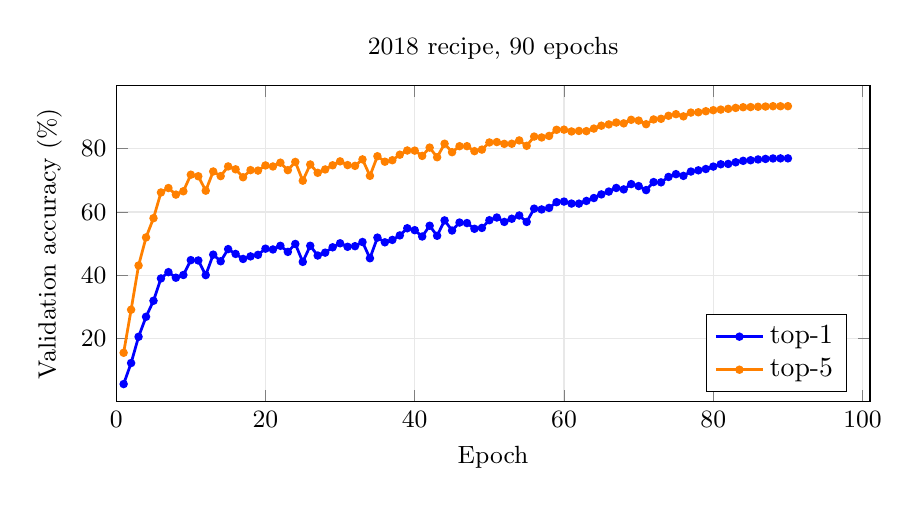
\begin{tikzpicture}
\begin{axis}[
    width=0.92\linewidth, height=5.6cm,
    xlabel={Epoch}, ylabel={Validation accuracy (\%)},
    xmin=0, xmax=101, ymin=0, ymax=100,
    xtick={0,20,40,60,80,100},
    ytick={20,40,60,80},
    legend pos=south east,
    legend cell align={left},
    grid=major, grid style={gray!18},
    tick label style={font=\small},
    label style={font=\small},
    title style={font=\small},
    every axis plot/.append style={line width=1pt, mark size=1pt},
    title={2018 recipe, 90 epochs},
]
\addplot[blue, mark=*, mark options={fill=blue}] coordinates {
(1,5.62) (2,12.26) (3,20.56) (4,26.88) (5,31.94) (6,39.00) (7,40.99) (8,39.22) (9,40.09) (10,44.78) (11,44.68) (12,40.05) (13,46.52) (14,44.43) (15,48.27) (16,46.74) (17,45.16) (18,45.97) (19,46.45) (20,48.40) (21,48.15) (22,49.31) (23,47.39) (24,49.90) (25,44.23) (26,49.32) (27,46.24) (28,47.15) (29,48.84) (30,50.11) (31,49.00) (32,49.19) (33,50.51) (34,45.38) (35,51.90) (36,50.42) (37,51.17) (38,52.60) (39,54.86) (40,54.25) (41,52.25) (42,55.65) (43,52.48) (44,57.34) (45,54.14) (46,56.66) (47,56.50) (48,54.69) (49,54.96) (50,57.40) (51,58.25) (52,56.86) (53,57.86) (54,58.89) (55,56.85) (56,61.05) (57,60.80) (58,61.29) (59,63.09) (60,63.29) (61,62.66) (62,62.64) (63,63.49) (64,64.41) (65,65.56) (66,66.45) (67,67.59) (68,67.14) (69,68.81) (70,68.19) (71,66.92) (72,69.45) (73,69.37) (74,71.08) (75,71.96) (76,71.41) (77,72.78) (78,73.17) (79,73.58) (80,74.35) (81,75.08) (82,75.18) (83,75.71) (84,76.16) (85,76.35) (86,76.60) (87,76.77) (88,76.91) (89,76.94) (90,76.95)
};
\addlegendentry{top-1}
\addplot[orange, mark=*, mark options={fill=orange}] coordinates {
(1,15.51) (2,29.11) (3,43.08) (4,51.96) (5,58.04) (6,66.17) (7,67.57) (8,65.49) (9,66.55) (10,71.78) (11,71.30) (12,66.73) (13,72.80) (14,71.34) (15,74.40) (16,73.49) (17,70.98) (18,73.23) (19,73.08) (20,74.71) (21,74.38) (22,75.58) (23,73.22) (24,75.82) (25,69.89) (26,75.01) (27,72.38) (28,73.44) (29,74.76) (30,76.00) (31,74.82) (32,74.57) (33,76.62) (34,71.42) (35,77.62) (36,75.88) (37,76.36) (38,78.10) (39,79.43) (40,79.39) (41,77.73) (42,80.35) (43,77.30) (44,81.57) (45,78.90) (46,80.79) (47,80.80) (48,79.23) (49,79.71) (50,81.97) (51,82.10) (52,81.53) (53,81.57) (54,82.62) (55,80.91) (56,83.83) (57,83.55) (58,84.03) (59,85.97) (60,86.02) (61,85.45) (62,85.61) (63,85.55) (64,86.36) (65,87.27) (66,87.68) (67,88.27) (68,88.01) (69,89.13) (70,88.89) (71,87.74) (72,89.24) (73,89.45) (74,90.40) (75,90.91) (76,90.22) (77,91.42) (78,91.51) (79,91.84) (80,92.17) (81,92.36) (82,92.60) (83,92.89) (84,93.11) (85,93.16) (86,93.25) (87,93.33) (88,93.43) (89,93.42) (90,93.44)
};
\addlegendentry{top-5}
\end{axis}
\end{tikzpicture}
\end{center}

\noindent ResNet-50 / ImageNet-1k validation accuracy per epoch on the
\textbf{2018} recipe, four 4060\,Ti cards, on the same axes as the A3 curve in
\S\ref{sec:r50_phase4} below. It shows the three-part shape ResNet-34 does: a
fast climb, a long shallow middle, and a final lift as the cosine anneals.

\medskip\noindent Against A3 the two are closer through the middle than the
$+1.31$ endpoint gap suggests. From roughly epoch~25 they trade the lead
repeatedly, and A3 does not hold it outright until epoch~86; at the matched
epoch~90 A3 leads by $0.77$ ($77.72$ against $76.95$), and its remaining ten
epochs of anneal add the rest. A3 also \emph{starts} far lower --- $0.32\%$ at
epoch~1 against $5.62\%$ here --- because BCE over mixup targets gives almost
no signal until the logits separate. \emph{Compare the middles with care:} the
schedules are different lengths, so at a shared epoch index the two cosines are
at different points in their decay. The endpoints are what the $+1.31$ is
measured from.

\textbf{What the re-run corrected, and what it was worth.} Beyond the
protocol change above, two optimizer corrections read out of \texttt{timm}'s
own source went in: LAMB's gradient clip, which \texttt{timm} enables by
default (\texttt{max\_grad\_norm} $= 1.0$) and we did not, and its guard
excluding the \texttt{no\_weight\_decay} group from layer adaptation, which we
had been applying to every parameter. Those two, the padding fix and the new
evaluation are together what moved this section's ResNet-50 onto
\texttt{timm}'s own footing --- a fidelity correction, not a recipe change,
which is why the $78.26\%$ is quotable against \texttt{timm}'s $78.05\%$
rather than an improvement on it.

\prosesection{The PJRT lowerer}
\label{sec:r50_phase4}

The same recipe on the \emph{verified} codegen path, which is not a
hand-written emitter but \texttt{pretty(provenGraph)}, the rendered MLIR
the proofs reason about, lowered through \texttt{ffi/pjrt\_ffi.c} to XLA
over the PJRT C API with no Python at run time. The artifact is
\texttt{resnet50in160\_lambaccdp8x64wxclipbce\_train\_step}: LAMB $\times$
BCE-with-logits $\times$ gradient accumulation $k=8$, four replicas at
per-replica batch 64 for an effective batch of 2048, train@160 /
eval@224.

\begin{center}
\begin{tabular}{l l l r r r r}
\hline
GPU & Recipe & BN group & Per epoch & Total & Val top-1 & Val top-5 \\
\hline
4$\times$ 3060 (bf16)    & 2018 (90 ep)    & Ghost-BN (64) & $\sim$20.5 min & $\sim$30.7 hr & $\mathbf{77.07\%}$ & $\mathbf{93.48\%}$ \\
4$\times$ 4060 Ti (fp32)  & RSB-A3 (100 ep) & Ghost-BN (64) & $\sim$19.2 min & $\sim$32.1 hr & $\mathbf{77.91\%}$ & $\mathbf{93.84\%}$ \\
\hline
\end{tabular}
\end{center}

\noindent The first row is the same network on the \emph{2018} recipe, and it
is the row that makes the comparison below a controlled
one: it is bit-for-bit
the ResNet-34 configuration of \S\ref{sec:r34_phase4} with the bottleneck
backbone substituted, so the only difference between it and the A3 row is the
recipe. It runs with:

\begin{verbatim}
CUDA_VISIBLE_DEVICES=0,1,2,3 PJRT_REPLICAS=4 LEAN_MLIR_REPLICAS=4 \
  SHIM_WORKERS=8 PJRT_FFI_RESIDENT=1 \
  LEAN_MLIR_VARIANT=momdp64bf16 LEAN_MLIR_BATCH=64 LEAN_MLIR_EPOCHS=90 \
  LEAN_MLIR_RECIPE=2018 LEAN_MLIR_BASE_LR_U=100000 \
  .lake/build/bin/resnet50-imagenet-verified data
\end{verbatim}

\noindent \textbf{\texttt{LEAN\_MLIR\_RECIPE} selects the augmentation.}
\texttt{shimScript} is a field on the network, not on the recipe, so the
$224^2$ spec has one shim per recipe and picking the wrong one trains the
right optimizer on the wrong data. \texttt{scripts/jobs/} encodes that and the
schedule knobs as refusing prechecks.

\textbf{How to quote these.} The A3 row lands $0.35$ points behind the JAX
reference above ($78.26\%$ / $93.79\%$) and $0.14$ behind \texttt{timm}'s own
$78.05\%$, measured over the same $50{,}000$ images under the same protocol.
The recipe is not yet A3 to the letter --- the ledger below is what is in and
what is still out --- so it is \emph{the A3 recipe on the verified path, with
these deltas}, rather than ``RSB-A3 reproduced''. The 2018 row needs no such
hedge: it is the recipe in full, and it lands $0.12$ points \emph{ahead} of its
own JAX reference.

\begin{center}
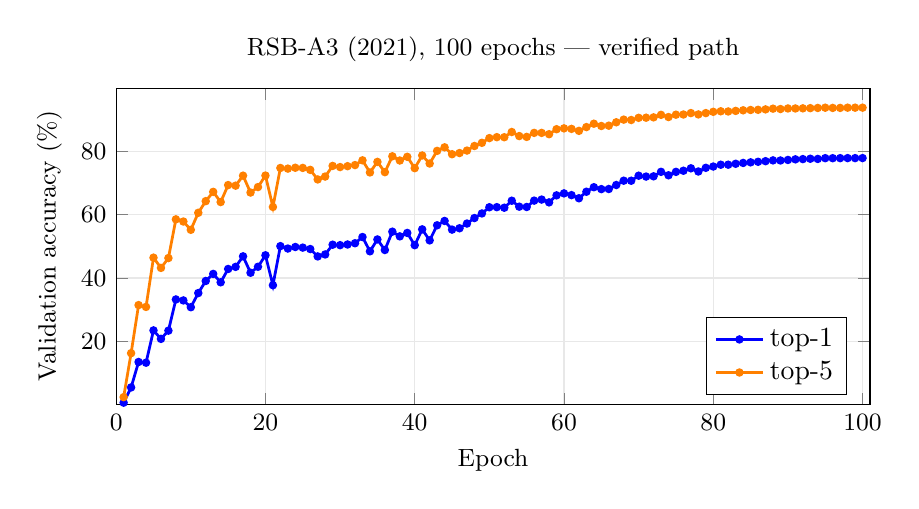
\begin{tikzpicture}
\begin{axis}[
    width=0.92\linewidth, height=5.6cm,
    xlabel={Epoch}, ylabel={Validation accuracy (\%)},
    xmin=0, xmax=101, ymin=0, ymax=100,
    xtick={0,20,40,60,80,100},
    ytick={20,40,60,80},
    legend pos=south east,
    legend cell align={left},
    grid=major, grid style={gray!18},
    tick label style={font=\small},
    label style={font=\small},
    title style={font=\small},
    every axis plot/.append style={line width=1pt, mark size=1pt},
    title={RSB-A3 (2021), 100 epochs --- verified path},
]
\addplot[blue, mark=*, mark options={fill=blue}] coordinates {
(1,0.61) (2,5.43) (3,13.47) (4,13.24) (5,23.45) (6,20.77) (7,23.37) (8,33.23) (9,32.92) (10,30.78) (11,35.25) (12,39.07) (13,41.30) (14,38.65) (15,42.86) (16,43.53) (17,46.86) (18,41.67) (19,43.56) (20,47.19) (21,37.73) (22,50.08) (23,49.32) (24,49.81) (25,49.61) (26,49.17) (27,46.83) (28,47.45) (29,50.53) (30,50.39) (31,50.60) (32,51.00) (33,52.96) (34,48.45) (35,52.19) (36,48.86) (37,54.65) (38,53.17) (39,54.25) (40,50.38) (41,55.38) (42,51.90) (43,56.67) (44,58.04) (45,55.30) (46,55.73) (47,57.22) (48,58.96) (49,60.41) (50,62.37) (51,62.40) (52,62.22) (53,64.43) (54,62.55) (55,62.45) (56,64.46) (57,64.80) (58,63.91) (59,66.13) (60,66.75) (61,66.20) (62,65.21) (63,67.27) (64,68.70) (65,68.10) (66,68.14) (67,69.40) (68,70.76) (69,70.75) (70,72.34) (71,72.07) (72,72.15) (73,73.56) (74,72.47) (75,73.55) (76,73.91) (77,74.68) (78,73.67) (79,74.83) (80,75.24) (81,75.81) (82,75.82) (83,76.11) (84,76.37) (85,76.56) (86,76.74) (87,76.93) (88,77.18) (89,77.15) (90,77.32) (91,77.51) (92,77.59) (93,77.70) (94,77.64) (95,77.88) (96,77.87) (97,77.89) (98,77.90) (99,77.90) (100,77.91)
};
\addlegendentry{top-1}
\addplot[orange, mark=*, mark options={fill=orange}] coordinates {
(1,2.36) (2,16.25) (3,31.45) (4,30.87) (5,46.44) (6,43.20) (7,46.31) (8,58.55) (9,57.86) (10,55.24) (11,60.62) (12,64.30) (13,67.23) (14,64.01) (15,69.38) (16,69.19) (17,72.35) (18,67.02) (19,68.75) (20,72.39) (21,62.46) (22,74.78) (23,74.58) (24,74.85) (25,74.80) (26,74.18) (27,71.16) (28,72.07) (29,75.43) (30,75.07) (31,75.35) (32,75.70) (33,77.20) (34,73.37) (35,76.71) (36,73.46) (37,78.48) (38,77.14) (39,78.31) (40,74.72) (41,78.73) (42,76.19) (43,80.19) (44,81.31) (45,79.13) (46,79.50) (47,80.28) (48,81.73) (49,82.73) (50,84.22) (51,84.52) (52,84.50) (53,86.15) (54,84.87) (55,84.60) (56,85.87) (57,85.87) (58,85.46) (59,87.03) (60,87.30) (61,87.14) (62,86.51) (63,87.70) (64,88.77) (65,88.05) (66,88.15) (67,89.22) (68,90.06) (69,89.94) (70,90.63) (71,90.67) (72,90.78) (73,91.57) (74,90.88) (75,91.62) (76,91.68) (77,92.13) (78,91.71) (79,92.13) (80,92.53) (81,92.70) (82,92.64) (83,92.82) (84,93.01) (85,93.11) (86,93.16) (87,93.30) (88,93.52) (89,93.41) (90,93.59) (91,93.59) (92,93.63) (93,93.69) (94,93.75) (95,93.83) (96,93.76) (97,93.76) (98,93.84) (99,93.84) (100,93.84)
};
\addlegendentry{top-5}
\end{axis}
\end{tikzpicture}
\end{center}

\noindent The verified path's own curve, on the same axes as the 2018 panel
above so the two can be read against each other. The endpoint is
$0.35$ points below the reference, but the shape getting there is not a
uniformly worse version of it: \emph{the verified path is ahead for 56 of the
100 epochs}, by as much as $14.3$ points at epoch~31, and the reference does
not take a durable lead until epoch~86 --- the same late-anneal window in
which A3 finally passes the 2018 recipe. Two runs can differ by a third of a
point at the end and by fourteen in the middle, so a mid-training comparison
between these panels says almost nothing about where they land.

\medskip\noindent What that gap is \emph{not} evidence of: the two paths
differ in more than the codegen. The reference normalises BatchNorm over
$512$ and this run over $64$, an eightfold difference in the statistic group
and much the largest known asymmetry between them, and this run is fp32
where the reference is bf16. Attributing the $0.35$ to the verified codegen
requires closing those first.

\medskip\noindent\emph{In, and in the $77.91\%$ above.} What this run
carries that a bare A3 transcription would not:

\begin{itemize}
  \item \texttt{wdExcludeNormBias} --- BN $\gamma/\beta$ and biases are not
    decayed; 54 decayed / 107 excluded of 161. Largest single contributor.
  \item \textbf{LAMB's gradient clip} (timm's \texttt{max\_grad\_norm}
    $= 1.0$ default), applied after the all-reduce \emph{and} after the
    accumulation, at threshold $kC$ (\texttt{Proofs.clipFactor\_accum}).
  \item The \texttt{no\_weight\_decay} group is not layer-adapted.
  \item BN running-statistic momentum compensated for accumulation.
    Evaluation-only.
  \item Evaluation scores all $50{,}000$ images. \textbf{Every top-1
    outside this chapter is still over $49{,}920$.}
  \item RandAugment Posterize, plus timm's validation protocol and
    resampler (appendix~\ref{app:data}).
  \item \emph{Verification:} the optimizer is tied to the reference at
    the \emph{update} as well as the gradient --- six variants to
    $\sim\!10^{-7}$.
\end{itemize}

\medskip\noindent\emph{Still out}, in rough order of expected effect:

\begin{itemize}
  \item Ghost-BN group 64 against the reference's 512; no collective
    touches the batch statistics. The largest known difference between the
    two paths, and \emph{untested}: the $-0.35$ points between them is its
    upper bound only if nothing else contributes.
  \item fp32, not bf16. The 2018 row above \emph{is} bf16, but the LAMB\,+\,BCE
    shape at $160^2$ still has no bf16 twin to run. (A2 and A1 at $224^2$ now
    have theirs, so this is A3's gap alone rather than the shared one it was.)
    Worth a measured $1.54\times$ on this network, so most of the $2.1\times$
    wall clock against the JAX row: a throughput lever, not a fidelity one.
  \item $0.08\%$ of each epoch dropped ($8 \nmid 5004$); structural to $k$.
  \item Mixup $\lambda$ drawn host-side from NumPy, so agreement is
    distributional, never per-step.
\end{itemize}

\prosesection{The two paths, side by side}

Both recipes have now been run on both lowerers, which is what makes this a
grid rather than a pair of anecdotes.

\begin{center}
\begin{tabular}{@{}l r r r @{\qquad} r r r@{}}
\hline
 & \multicolumn{3}{c}{\textbf{2018} (90 ep)} & \multicolumn{3}{c}{\textbf{RSB-A3} (100 ep)} \\
 & JAX & PJRT & $\Delta$ & JAX & PJRT & $\Delta$ \\
\hline
top-1        & $76.95$ & $\mathbf{77.07}$ & $+0.12$ & $78.26$ & $\mathbf{77.91}$ & $-0.35$ \\
top-5        & $93.44$ & $\mathbf{93.48}$ & $+0.04$ & $93.79$ & $\mathbf{93.84}$ & $+0.05$ \\
precision    & bf16 & bf16 & & bf16 & fp32 & \\
box          & 4060\,Ti & 3060 & & 4060\,Ti & 4060\,Ti & \\
wall clock   & $24.0$\,h & $30.7$\,h & & $15.1$\,h & $32.1$\,h & \\
\hline
\end{tabular}
\end{center}

\noindent \textbf{The two lowerers agree within $0.35$ points of top-1 on both
recipes}, and both agree to within $0.05$ on top-5. That is the claim the grid
licenses and the reason the second lowerer exists: with one backend the proofs
decorate a code generator and nothing checks the generator, while a second
independent lowering makes the verified path the artifact and JAX the oracle it
is checked against.

\medskip\noindent \textbf{And the recipe delta replicates.} A3 beats 2018 by
$+1.31$ points on the JAX lowerer and by $+0.84$ on the verified one. Agreement
at a single configuration can be a coincidence of that configuration; a
\emph{difference} that reproduces across two independent implementations is
harder to arrange by accident, and it is what a one-row comparison cannot show.

\medskip\noindent \textbf{What this is not evidence of.} Each cell is one run
at one seed, and $0.35$ points is inside what seed variance alone produces on
ImageNet --- the agreement is consistent with the lowerers matching, not proof
that they do. The A3 column trains at $160$ and evaluates at $224$ while the
2018 column does both at $224$, so the recipe delta confounds resolution with
recipe, by A3's own design. And the PJRT column is not internally uniform: its
2018 entry is bf16 on the four-3060 box, its A3 entry fp32 on the four-4060\,Ti
box. Neither difference touches the within-recipe comparison, which is the one
the table is for, but both would matter to anyone reading down the PJRT column.

\subsection*{What A3 changes from the 2018 recipe}
\label{sec:r50_a3_vs_2018}

The 2018-recipe row above is the original paper's SGD-with-momentum plus the
``bag of tricks'' polish (cosine schedule, warmup, label smoothing,
random-resized-crop). RSB-A3 is the \emph{2021} ``ResNet Strikes Back'' recipe
(Wightman et al.). Both rows are ResNet-50, which is the point: every knob that
A3 sets differently is one lever of the three-year jump in how these networks
are trained, and holding the architecture fixed is what stops the comparison
confounding the recipe with the backbone. The spec, the render and the entry
point are identical between them, and only the arguments differ. Here is the
full diff:

\begin{center}
\begin{tabular}{@{}l p{2.9cm} p{3.2cm} p{6.3cm}@{}}
\hline
Knob & ResNet-50 (2018) & RSB-A3 (2021) & What the A3 choice buys \\
\hline
Backbone      & bottleneck, 25.6\,M    & bottleneck, 25.6\,M          & unchanged, which is what makes the rest of this table a recipe diff \\
Optimizer     & SGD + momentum $0.9$   & LAMB                          & layer-wise adaptive LR, designed for very large batches \\
Effective batch & 256                  & 2048 ($512\times4$ accum)     & the large-batch regime LAMB targets; grad-accum fits it on 16\,GB \\
Peak LR       & $0.1$                  & $0.008$ @ bs2048              & LAMB's trust-ratio scale --- not comparable to SGD's $0.1$ \\
Epochs        & 90                     & 100                           & essentially the same budget (A3 is the cheap RSB tier) \\
Loss          & softmax cross-entropy  & BCE-with-logits, multi-hot    & treats classes independently; matches mixed soft targets \\
Label smoothing & $0.1$                & $0.0$                         & subsumed --- BCE over soft mixup labels already softens targets \\
Augmentation  & RRC + hflip            & RRC + hflip                   & unchanged, and it is the BASE both recipes train on; the two rows below are what A3 layers on top of it \\
Mixup / CutMix & none                  & $\alpha\,0.1$ / $\alpha\,1.0$ & interpolate/paste samples $\to$ soft multi-hot targets, strong regularizer \\
RandAugment   & none                   & \texttt{m6 N2 mstd0.5 inc1}   & automated heavy color+geometric augmentation policy \\
Weight decay  & $10^{-4}$, all params  & $0.02$, skip BN $\gamma/\beta$ + bias & $200\times$ stronger, but never decays scale/shift/bias params \\
Train / eval res & $224$ / $224$        & $160$ / $224$                 & FixRes: train at cheap low res ($\sim$2$\times$ faster/step), test at high res --- the train/test gap helps \\
BN statistics & global over batch      & Ghost-BN over 512             & side-effect of grad-accum (each micro-step normalizes its own 512); a single big-memory card would remove it \\
\hline
\end{tabular}
\end{center}

\noindent What carries over unchanged: cosine LR decay, the 5-epoch
warmup, the base augmentation in the row above, bf16 matmul and
convolution, and running-BN evaluation. The through-line
of the 2018$\to$2021 shift is \emph{regularize harder, train bigger}:
heavier augmentation (RandAugment + Mixup + CutMix), a loss that accepts
soft targets (BCE), an order-of-magnitude more weight decay applied
selectively, and a large-batch optimizer (LAMB) to make the longer,
noisier training converge, with FixRes buying back the compute the
extra epochs would cost. Every one of these is a one-line
\texttt{TrainConfig} change on the same verified backbone.

\section{Side quest: RSB-A2 and RSB-A1}
\label{sec:r50_a2_a1_cost}

A3 is the cheap tier. The other two are recipes --- \texttt{a2-accum} and
\texttt{a1} --- and both now render on the verified path:

\begin{center}
\begin{tabular}{@{}l c c l l l@{}}
\hline
tier & epochs & train res & verified render & verified wall clock & top-1 \\
\hline
A3 (\texttt{rsb-faithful}) & 100 & $160$ & shipped, and run & $\sim$32.1 hr & $\mathbf{77.91\%}$ \\
A2 (\texttt{a2-accum})     & 300 & $224$ & rendered, EMA + sd & \texttt{[todo]} & $79.8\%$ (paper) \\
A1 (\texttt{a1})           & 600 & $224$ & rendered, EMA + sd & \texttt{[todo]} & $80.4\%$ (paper) \\
\hline
\end{tabular}
\end{center}

\noindent Twenty-four artifacts: each tier at one and four replicas, in both
precisions, at either factorisation of the effective batch $2048$ ---
$512\times4$ on the reference, $8\times64$ or $4\times128$ here. \textbf{A1 is not
``the same render as A2''}: the decay is baked, so A1's $0.01$ against A2's
$0.02$ is a re-render, and the two are kept apart so that one line among
$18{,}000$ cannot be lost.

\medskip\noindent \textbf{The two regularisers these renders used to be missing
are now in them.} The ledger \S\ref{sec:r50_phase4} keeps for A3, before anything
is run:

\begin{center}
\begin{tabular}{@{}p{0.45\linewidth} p{0.47\linewidth}@{}}
\hline
\emph{In} & \emph{Still out}, worst first \\
\hline
\texttt{wdExcludeNormBias}; LAMB's clip at $kC$, after both the all-reduce and the accumulation
  & \textbf{Ghost-BN group} $64$ against the reference's $\mathbf{512}$ --- an $8\times$ gap, and only half of it is reachable here \\[2pt]
BCE-with-logits over Mixup/CutMix soft labels
  & Repeated augmentation is stream-level, not per-batch \\[2pt]
Accumulation to LAMB's design batch of $2048$, at $k=8$ or at the reference's own $k=4$
  & Nothing trained --- no epoch of either tier has run here \\[2pt]
\textbf{Model EMA} at decay $0.9999$ --- a \emph{fifth} blob region, $[\theta|m|v|G|E]$
  & \\[2pt]
\textbf{Stochastic depth} $0.05$ --- sixteen sites, one per bottleneck, on the residual branch
  & \\[2pt]
Repeated augmentation $3\times$; both tiers, one and four replicas
  & \emph{fp32 and bf16 do not both exist for every render} --- see the memory table \\[2pt]
A1's own decay and own shim, which the driver refuses to start without
  & \\[2pt]
Optimizer tied at the update, seven variants to ${\sim}10^{-7}$ & \\
\hline
\end{tabular}
\end{center}

\noindent \textbf{Both were structural, and A3 met neither} --- its recipe
switches both \emph{off}. The shadow and the accumulator used to be the
\emph{same} fourth region of $[\theta|m|v|\cdot]$, and accumulation is not
optional at $224^2$ on a $16$\,GB card: EMA was unreachable, not unrendered.

\medskip\noindent Stochastic depth's site sits on the residual \emph{branch}, and
\textbf{no structural check can tell that from a site on the block output}: at an
all-ones mask $1 \odot (b+x)$ and $1 \odot b + x$ agree bit-for-bit, so a
misplaced render matches on names, operation count and arity and passes every
endpoint gate. Moving all sixteen separates them by eight orders of magnitude at
a real mask, and by exactly zero at an all-ones one. The reference had the same
feature wrong the other way round --- a scalar \texttt{bernoulli} for the whole
batch where timm's is per \emph{sample}, same expectation, which is why it
survived.

\medskip\noindent \textbf{What each render costs on one card}, from XLA's own
\texttt{peak\_memory\_in\_bytes}:

\begin{center}
\begin{tabular}{@{}l l c r r r@{}}
\hline
render & precision & BN group & peak & of $11.68$ & of $15.11$ \\
\hline
$8\times64$             & fp32 & $64$  & $6.18$\,GiB  & $53\%$ & $41\%$ \\
$8\times64$             & bf16 & $64$  & $4.32$\,GiB  & $37\%$ & $29\%$ \\
$8\times64$ + EMA + sd  & fp32 & $64$  & $6.37$\,GiB  & $55\%$ & $42\%$ \\
$4\times128$ + EMA + sd & bf16 & $128$ & $8.09$\,GiB  & $69\%$ & $54\%$ \\
$4\times128$ + EMA + sd & fp32 & $128$ & $11.91$\,GiB & over   & $79\%$ \\
\hline
\end{tabular}
\end{center}

\noindent The fifth region costs $0.19$\,GiB, all of it arguments; stochastic
depth costs nothing measurable. \textbf{And the two budget columns are the point.}
A PJRT client created with no allocator options takes the plugin's $0.75$ default
--- which is where $11.68$ comes from, and four gigabytes of a $16$\,GB card with
it. \texttt{XLA\_PYTHON\_CLIENT\_MEM\_FRACTION} does not change it: the plugin
never reads that variable, JAX's Python layer does, and passes
\texttt{memory\_fraction} as a \emph{create option}. The shim now passes it too.
\textbf{The largest render goes from not fitting to $79\%$, and nothing about the
hardware moved.}

\medskip\noindent \textbf{Which leaves the batch-norm group, larger than it
looks.} Nothing here all-reduces activation statistics, so each replica
normalises over its own $64$; the reference's \texttt{jnp.mean} reduces over a
\emph{mesh-sharded} axis, so XLA inserts one and its group is the full $512$. Its
per-device tensor is $128$, and only the group is the statistic. Half the gap is
a re-render, $k=4$ at $128$ per device; the last $4\times$ needs synchronised
batch-norm --- a new operator, a changed backward, a variance that does not
average, and $53$ collectives a step.

\medskip\noindent \textbf{What the phase-2 peers cost, measured.}
\texttt{jax/scripts/step\_probe.py} on four 4060\,Ti, bf16, with A3 as the
control:

\begin{center}
\begin{tabular}{@{}l r r r r@{}}
\hline
phase-2 tier & train res & ms/step & min/epoch & full schedule \\
\hline
A3 (100 ep) & $160$ & $715$     & $7.5$  & $12.4$\,h \\
A2 (300 ep) & $224$ & $1{,}368$ & $14.3$ & $71.3$\,h (3.0\,d) \\
A1 (600 ep) & $224$ & $1{,}368$ & $14.3$ & $142.5$\,h (5.9\,d) \\
\hline
\end{tabular}
\end{center}

\noindent A1 and A2 share a step figure because the trainers differ in three
constants. Compute-only, so a lower bound: scaling by the one tier where both
paths have a number ($19.2$ verified minutes per epoch against $7.5$) puts a
verified A2 near seven days and A1 near fifteen.

\chapter{MobileNetV2}
\label{chap:depthwise}

\prosesection{A standard conv does two jobs at once}

A standard 3$\times$3 convolution from \(C_\text{in}\) channels to
\(C_\text{out}\) channels computes, for every output cell:

\[
y_{c_\text{out},\,i,\,j}
\;=\;
\sum_{c_\text{in},\,k_h,\,k_w}
W_{c_\text{out},\,c_\text{in},\,k_h,\,k_w}
\cdot
x_{c_\text{in},\,i+k_h,\,j+k_w}.
\]

That sum is doing two things. The \(k_h, k_w\) part is
\emph{spatial mixing}: it combines a pixel with its neighbors. The
\(c_\text{in}\) part is \emph{cross-channel mixing}: it combines
the \(C_\text{in}\) channels into each of \(C_\text{out}\) new
channels. Both happen inside the same kernel and at the same cost
\(C_\text{in} \times C_\text{out} \times k^2\) weights per layer.

Howard et al.\ 2017 (MobileNetV1, then V2 in
\href{https://arxiv.org/abs/1801.04381}{arXiv:1801.04381})
asked: what if we factored those two responsibilities and only
paid the full cost of one of them? The spatial mixing is locally
information-rich and benefits from a real \(3 \times 3\)
neighborhood. The channel mixing can be approximated by a much
cheaper operation. If we separate them, we get parameter
efficiency without losing much expressive power.

\section{Run it first}
\label{sec:mnv2_runit}

Before the factorization, train the factorized network. Four commands,
and about the same GPU time Chapter~\ref{chap:residual} asked for:

\begin{verbatim}
lake exe cache get                            # Mathlib oleans, ~30 s
./download_imagenette.sh                      # 330 MB dl, 2.4 GB unpacked
lake build mobilenetv2-verified-adam
./.lake/build/bin/mobilenetv2-verified-adam data
\end{verbatim}

On one RTX 4060 Ti (CUDA 12.9), from
\texttt{runs/2026-08-12-mnv2-imagenette-xla-cuda/}. XLA's startup banner
is removed, the network description line is wrapped, and the middle of
the run is elided:

\begin{verbatim}
[pjrt_ffi] XLA backend: PJRT 0.112, 1 device(s)
[pjrt_ffi] compiled verified_mlir/mobilenetv2_adam_train_step.mlir
             (@mobilenetv2_adam_train_step, 581 outputs, 1 replica) in 8101 ms
[pjrt_ffi] compiled verified_mlir/mobilenetv2_fwd.mlir
             (@mobilenetv2_fwd, 1 outputs, 1 replica) in 665 ms
[pjrt_ffi] compiled verified_mlir/mobilenetv2_fwd_eval.mlir
             (@mobilenetv2_fwd_eval, 1 outputs, 1 replica) in 250 ms
MobileNetV2 on Imagenette 224² (stem-s2 → 17 inverted-residual blocks,
  full-paper [t,c,n,s] config, stride-2 depthwise downsamples 224→7 →
  head conv-BN-relu6 → GAP → dense)
  via the VERIFIED renderer → XLA/PJRT → GPU
  train 9469, val 3925; bs 32, MobileNetV2 adam
    (cosine+warmup 3ep, baseLR 0.001000), He init
  running-stats BN: 52 layers, 34112 stat floats → eval via @mobilenetv2_fwd_eval
Epoch 1/80: loss=2.121050 lr=0.000333
  epoch 1: val_acc = 947/3925 = 24.127389%  top5 = 2392/3925 = 60.942675%
Epoch 2/80: loss=1.784318 lr=0.000667
  epoch 2: val_acc = 680/3925 = 17.324841%  top5 = 2357/3925 = 60.050955%
Epoch 3/80: loss=1.590689 lr=0.001000
  epoch 3: val_acc = 1596/3925 = 40.662420%  top5 = 3423/3925 = 87.210191%
Epoch 4/80: loss=1.446373 lr=0.001000
  epoch 4: val_acc = 1851/3925 = 47.159236%  top5 = 3428/3925 = 87.337580%
Epoch 79/80: loss=0.517682 lr=0.000000
  epoch 79: val_acc = 3506/3925 = 89.324841%  top5 = 3874/3925 = 98.700637%
Epoch 80/80: loss=0.517213 lr=0.000000
  epoch 80: val_acc = 3503/3925 = 89.248408%  top5 = 3873/3925 = 98.675159%
done (trained MobileNetV2 adam + cosine/warmup via packed threading).
\end{verbatim}

Eighty epochs at about 26 seconds each, thirty-five minutes in total, and
\textbf{89.25\%} top-1 with \textbf{98.68\%} top-5 on Imagenette's
3,925-image validation split. The best epoch reached $89.32\%$. Set that
against Chapter~\ref{chap:residual}, which ran the same data, the same
recipe and the same number of epochs through a network with
$9.5\times$ the parameters and finished at $89.71\%$ top-1 and $98.27\%$
top-5. MobileNetV2 gives up less than half a point of top-1, picks up
four tenths of top-5, and does it in thirty-five minutes against an hour
and a half.

Epoch 2 is worth a glance before moving on. Validation accuracy
\emph{falls}, from $24.1\%$ to $17.3\%$, while the training loss drops
normally from $2.12$ to $1.78$. That is the warmup: the learning rate is
still climbing toward its peak at epoch 3, and the BatchNorm running
statistics are two epochs old and averaging over a network whose weights
are moving fast. The evaluation forward is using statistics that no
longer describe the thing being evaluated. It corrects itself by epoch 3
and never recurs.

Depthwise separability doesn't weaken it. That run did not execute a
reimplementation of the network this chapter describes. It executed
\texttt{verified\_mlir/mobilenetv2\_adam\_train\_step.mlir}, which is
\texttt{pretty(provenGraph)} off the renderer. Every depthwise
convolution in it backpropagates by the rule
Theorem~\ref{ax:depthwise_has_vjp3} proves, every pointwise convolution
by Chapter~\ref{chap:cnn}'s, every BatchNorm by Chapter~\ref{chap:bn}'s,
and every residual skip by Chapter~\ref{chap:residual}'s additive
fan-in. Those per-operation theorems are unconditional and hold at any
width or depth, so they cover all seventeen blocks.

One scope note, because this is the chapter where the distinction starts
to bite. The theorem that folds those rules into a single statement about
the \emph{whole} network is \texttt{mobilenetv2\_full\_has\_vjp\_at}, in
\texttt{MobileNetV2FullVJP.lean}, and it covers the stem, all seventeen
bottlenecks and the head. What ties the full 17-block spec
to the paper's architecture is a separate denotational result about the
forward, \texttt{mobilenetv2Verified\_denote\_eq}, with
\texttt{mobilenetv2Verified\_fwd\_faithful} above it.

The full-depth fold is \emph{pointwise}. It holds at a given input, and
it carries one side condition per activation site saying that the value
entering relu6 is neither $0$ nor $6$. There are thirty-five such sites,
and the reason for every one of them is that relu6 has two kinks. The
network is differentiable away from them and is not differentiable at
them, so a statement quantified over all inputs would be false.
Chapter~\ref{chap:se} does fold EfficientNet-B0 over all inputs with
\texttt{efficientnetForwardB\_full\_has\_vjp}, and it can do that because
swish is smooth everywhere. The axis that moved here was the depth, from
two blocks to seventeen, and not the pointwise-to-global one.

The three compile lines are the same three Chapter~\ref{chap:residual}
showed, and for the same reason. \texttt{@mobilenetv2\_fwd\_eval} is a
separate forward because BatchNorm evaluates differently than it trains,
and \texttt{running-stats BN: 52 layers, 34112 stat floats} is the driver
threading the running averages out of the train step and into it. This
network has 52 BatchNorms against ResNet-34's 36, which is what a block
built from three convolutions instead of two costs.

To run this net alongside the other six at the same scale and recipe:

\begin{verbatim}
lake run imagenette
\end{verbatim}

That is the whole Part-I tier at $224^2$, and it is an afternoon rather
than the minute \texttt{lake run mnist} takes.

\prosesection{Depthwise: one kernel per channel, no cross-channel sum}

A \emph{depthwise} convolution does the spatial half on its own,
per channel. Each output channel comes from one input channel, with
its own \(k \times k\) kernel:

\[
y_{c,\,i,\,j}
\;=\;
\sum_{k_h,\,k_w}
W_{c,\,k_h,\,k_w}
\cdot
x_{c,\,i+k_h,\,j+k_w}.
\]

Only one summation level (over the kernel positions), not two. No
mixing between channels at all. Channel \(c\) of the output only
ever looks at channel \(c\) of the input. The weight tensor is
shape \([C, k, k]\) instead of \([C_\text{out}, C_\text{in}, k, k]\):

\[
\text{depthwise weights: } C \times 3 \times 3
\quad\text{vs}\quad
\text{standard weights: } C_\text{out} \times C_\text{in} \times 3 \times 3.
\]

For a typical \(C_\text{in} = C_\text{out} = 64\) layer, that is 576
weights against 36{,}864, a 64$\times$ reduction. The Jacobian
from Chapter \ref{chap:cnn} simplifies in step: one fewer \(\Sigma\)
level means the depthwise input-VJP is a slightly simpler
reversed-kernel convolution, the weight VJP is a slightly simpler
transpose-trick, and the bias VJP is the same per-channel sum.
Theorems \ref{ax:depthwise_has_vjp3} through
\ref{ax:depthwise_bias_grad_has_vjp} prove the depthwise VJPs.

\prosesection{The depthwise-separable sandwich}

A depthwise conv alone never lets channels see each other. That is
a problem, because the whole point of stacking convolutions is to
build hierarchical features that combine information across channels.
The fix is to follow each depthwise with a \emph{pointwise}
\(1 \times 1\) convolution, which is purely cross-channel mixing
(no spatial structure, since each output pixel is a learned linear
combination of the same input pixel's channels). That two-step
combination,

\[
\text{depthwise}\ 3 \times 3
\quad \longrightarrow \quad
\text{pointwise}\ 1 \times 1,
\]

is called a \emph{depthwise-separable convolution}, and it is what
replaces the standard \(3 \times 3\) conv in MobileNet and
everywhere downstream. A standard \(3 \times 3\) over 64$\to$64
costs 36{,}864 weights. The separable version costs 576 (depthwise)
plus 4{,}096 (pointwise), for 4{,}672. Eight times fewer.

\prosesection{Inverted residual: depthwise at the wide point}

MobileNetV2 wraps the separable block in one more idea. ResNet's
bottleneck block is wide $\to$ narrow $\to$ wide (project down for
the expensive spatial conv, project back up for the residual).
MobileNetV2 flips it: \emph{narrow $\to$ wide $\to$ narrow}, with
the depthwise spatial conv at the wide expansion. The intuition
is that depthwise is so cheap that you can afford to make it
\emph{wider}. The narrow bottleneck channels carry the actual
information across the residual.

Concretely, an inverted-residual block with input channels \(C_\text{in}\),
output channels \(C_\text{out}\), and expansion ratio \(t\):

\begin{enumerate}
\item \(1 \times 1\) conv \(C_\text{in} \to t \cdot C_\text{in}\)
  (the expand)
\item \(3 \times 3\) depthwise at \(t \cdot C_\text{in}\) channels
  (the spatial mix at the wide point)
\item \(1 \times 1\) conv \(t \cdot C_\text{in} \to C_\text{out}\)
  (the project, narrowing back down)
\item Residual skip when \(C_\text{in} = C_\text{out}\) and stride
  equals 1
\end{enumerate}

This is the \texttt{.invertedResidualNB ic mid oc stride} primitive
in the spec, one layer constructor that emits all three convs, the
BN and relu6 between them, and the conditional residual add. It
takes the expanded width \texttt{mid} directly rather than the ratio
\(t\), so a block is written the way it is shaped rather than the way
it is parameterized, and the \texttt{NB} suffix says the three convs
carry no bias, since the BatchNorm immediately after each one
subsumes it. The VJP for the whole block composes the depthwise VJP
from this chapter with the standard conv2d VJPs from
Chapter~\ref{chap:cnn}, the BN VJP from Chapter~\ref{chap:bn}, and
the additive fan-in for the residual from
Chapter~\ref{chap:residual}. Once again there is no new math beyond
the foundation rules, only the depthwise primitive plus composition.

\prosesection{Stacking the blocks}

MobileNetV2 stacks 17 inverted-residual blocks across seven stages
(at depths 1, 2, 3, 4, 3, 3, 1) with widths progressing from 16 to
320 channels, then a final \(1 \times 1\) to 1280 channels, global
average pool, and a 1280-to-10 dense head. That is the same
stem-stages-head template as ResNet-34. Total: 2.24M parameters,
9.5$\times$ fewer than ResNet-34, at a modest accuracy cost
($89.25\%$ against ResNet-34's $89.71\%$ on Imagenette, both
measured in this book). For mobile and embedded deployment that
trade is the whole reason MobileNet exists.

\section{The theorems}

\begin{definition}[Depthwise conv forward]
  \label{ax:depthwiseConv2d}
  \lean{Proofs.depthwiseConv2d}
  \leanok
  Concrete per-channel cross-correlation.
\end{definition}

\begin{theorem}[Depthwise input VJP]
  \label{ax:depthwise_has_vjp3}
  \lean{Proofs.depthwise_has_vjp3}
  \leanok
  \uses{ax:depthwiseConv2d, ax:pdiv_add, ax:pdiv_const, ax:pdiv_mul, thm:pdiv_finset_sum, ax:pdiv_reindex, def:hasvjp3}
  \Prove{} \(\HasVJPthree\, \bigl(\mathrm{depthwiseConv2d}(W, b)\bigr)\),
  with the per-channel reversed-kernel backward
  \(dx_{c, h, w} = \sum_{k_h, k_w}
    W_{c,\, k_H - 1 - k_h,\, k_W - 1 - k_w} \cdot
    dy_{c,\, h + k_h - p,\, w + k_w - p}\).
\end{theorem}

\begin{proof}
\leanok
\emph{Sketch: the conv2d input VJP
(Theorem~\ref{ax:conv2d_has_vjp3}) with one fewer \(\Sigma\) level ---
depthwise has no cross-channel mixing, so the channel of every
\(v\)-read is forced to equal the output channel.}
\begin{enumerate}
  \item Define \(B(x, dy)_{c, h_i, w_i} :=
    \sum_{h_o, w_o} [\text{pad-valid}]\;
      W_{c, \hat{k}_h, \hat{k}_w} \cdot dy_{c, h_o, w_o}\)
    with reconstructed offsets
    \(\hat{k}_h = h_i + p_H - h_o\), \(\hat{k}_w = w_i + p_W - w_o\)
    --- same shape as the conv2d formula, minus the channel sum.
  \item \Suffices{} \(B\) matches the \(\pdiv_3\) contraction at every
    index. \pf{Definition~\ref{def:hasvjp3}.}
  \item The flattened forward is affine in \(v\): constant bias plus
    \(\sum_{k_h, k_w} W_{o(\mathrm{idx}), k_h, k_w} \cdot
      (\text{pad-conditional projection of } v)\), where the
    projection reads channel \(o(\mathrm{idx})\) itself.
    \pf{Unfold (Definition~\ref{ax:depthwiseConv2d}); steps and rules
    exactly as in Theorem~\ref{ax:conv2d_has_vjp3} step 4
    (Theorems~\ref{ax:pdiv_add}, \ref{ax:pdiv_const},
    \ref{thm:pdiv_finset_sum} \(\times 2\), \ref{ax:pdiv_mul},
    \ref{ax:pdiv_reindex}), with a double instead of triple sum.}
  \item Collapse: the channel component of the indicator forces
    \(c_o = c_i\) (channel mismatch zeroes every other term); per
    \((h_o, w_o)\) the remaining two-conjunct indicator
    (\(k_h + h_o = h_i + p_H\), \(k_w + w_o = w_i + p_W\)) collapses
    the \((k_h, k_w)\) sum.
    \pf{\texttt{Finset.sum\_eq\_single} on the decoded components.}
  \item \Qed{}
    \pf{What remains is \(B(x, dy)_{c_i, h_i, w_i}\) (equivalent to
    the reversed-kernel form under
    \(k_h \leftrightarrow k_H - 1 - k_h\)); with 2, done.}
\end{enumerate}
\end{proof}

\begin{theorem}[Depthwise weight VJP]
  \label{ax:depthwise_weight_grad_has_vjp3}
  \lean{Proofs.depthwise_weight_grad_has_vjp3}
  \leanok
  \uses{ax:depthwiseConv2d, ax:pdiv_add, ax:pdiv_const, ax:pdiv_mul, thm:pdiv_finset_sum, ax:pdiv_reindex, def:hasvjp3}
  \texttt{DepthwiseKernel} is definitionally
  \(\mathsf{Tensor3}\), so \(\HasVJPthree\) applies to the kernel
  directly --- no flatten bijection needed, unlike the conv2d weight
  VJP (Theorem~\ref{ax:conv2d_weight_grad_has_vjp}).
  \Prove{} \(\HasVJPthree\,
    \bigl(W \mapsto \mathrm{depthwiseConv2d}(W, b)\, x\bigr)\),
  with the per-channel transpose-trick backward
  \(dW_{c, k_h, k_w} = \sum_{h_o, w_o} [\text{pad-valid}]\;
    x_{c,\, k_h + h_o - p_H,\, k_w + w_o - p_W} \cdot dy_{c, h_o, w_o}\).
\end{theorem}

\begin{proof}
\leanok
\begin{enumerate}
  \item Define \(B(W, dy)_{c, k_h, k_w}\) as the formula above.
  \item \Suffices{} \(B\) matches the \(\pdiv_3\) contraction at every
    kernel index. \pf{Definition~\ref{def:hasvjp3}, applicable since
    the kernel is a \(\mathsf{Tensor3}\).}
  \item Per-\((c_o, h_o, w_o)\) Jacobian:
    \(\pdiv_3 = [c_o = c]\, \cdot (\text{pad-conditional } x
    \text{ term})\) --- a single channel equality where the conv2d
    weight VJP had a packed \(\varphi\)-comparison.
    \pf{At output \((c_o, h_o, w_o)\) the forward is
    \(b_{c_o} + \sum_{k_h, k_w} W_{c_o, k_h, k_w} \cdot
      x\text{-pad-term}\): affine decomposition and the same
    foundation-rule sequence as Theorem~\ref{ax:conv2d_weight_grad_has_vjp}
    step 4 (sum + constant + finite-sum \(\times 2\) + product +
    reindex rules).}
  \item \Qed{}
    \pf{Contract 3 with \(dy\): collapse the channel sum at
    \(c_o = c\) (\texttt{Finset.sum\_eq\_single}); the spatial sums
    survive, leaving exactly \(B\); with 2, done.}
\end{enumerate}
\end{proof}

\begin{theorem}[Depthwise bias VJP]
  \label{ax:depthwise_bias_grad_has_vjp}
  \lean{Proofs.depthwise_bias_grad_has_vjp}
  \leanok
  \uses{ax:depthwiseConv2d, ax:pdiv_add, ax:pdiv_const, ax:pdiv_reindex, def:hasvjp}
  \Prove{} \(\HasVJP\, \bigl(b \mapsto \mathrm{flatten}
    (\mathrm{depthwiseConv2d}(W, b)\, x)\bigr)\), with backward
  \(db_c = \sum_{h_i, w_i} dy_{\mathrm{flat}(c, h_i, w_i)}\).
\end{theorem}

\begin{proof}
\leanok
Same three steps as the conv2d bias VJP
(Theorem~\ref{ax:conv2d_bias_grad_has_vjp}), with input channel
\(=\) output channel throughout:
\begin{enumerate}
  \item As a function of \(b\), the flattened forward is
    \((\text{channel reindex of } b) + (\text{$W\!,x$ term constant in }
    b)\), so \(\pdiv = \delta_{c,\, \mathrm{chan}(\mathrm{idx})}\).
    \pf{Sum rule (Theorem~\ref{ax:pdiv_add}), reindex Jacobian
    (Theorem~\ref{ax:pdiv_reindex}), constant rule
    (Theorem~\ref{ax:pdiv_const}).}
  \item \Suffices{} \(db_c = \sum_{\mathrm{idx}} \pdiv \cdot
    dy_{\mathrm{idx}}\). \pf{Definition~\ref{def:hasvjp}.}
  \item \Qed{}
    \pf{Contract 1 with \(dy\); the Kronecker keeps channel \(c\)'s
    spatial positions (\texttt{Finset.sum\_eq\_single}).}
\end{enumerate}
\end{proof}

\section{Example: MobileNet V2 on Imagenette}
\label{sec:depthwise_mnv2_example}

Depthwise convolution on its own is rarely used directly. You
almost always see it wrapped in a \emph{depthwise-separable}
sandwich: $1 \times 1$ expand, $3 \times 3$ depthwise, $1 \times 1$
project, with a residual connection around the whole thing. That
sandwich is the inverted-residual block that defines MobileNet V2,
and it is how depthwise convolutions got their fame.

The point of depthwise is \emph{parameter efficiency}. A normal
$3 \times 3$ conv over 64 channels uses $3 \times 3 \times 64
\times 64 = 36864$ weights. A depthwise version uses $3 \times 3
\times 64 = 576$ weights. 64$\times$ fewer. The depthwise-separable
block recovers the missing cross-channel expressivity with the
surrounding $1 \times 1$ convs, at a combined cost far below a full
$3 \times 3$. MobileNet V2 is 17 of these blocks together.

\subsection*{The architecture}

The same vertical column as ResNet-34, now built from
inverted-residual blocks: a $3 \times 3$ stride-2 stem, seven stages of
\texttt{.invertedResidualNB} blocks (17 in all, widths $16$ to $320$,
expansion $t{=}6$ except the first), a $1 \times 1$ lift to 1280
channels, global average pool, and a dense head. There are \emph{no}
max-pools, since every downsample is folded into a strided block. The
inset shows one inverted-residual block: the cheap depthwise spatial mix
happens at the wide point.

\begin{center}
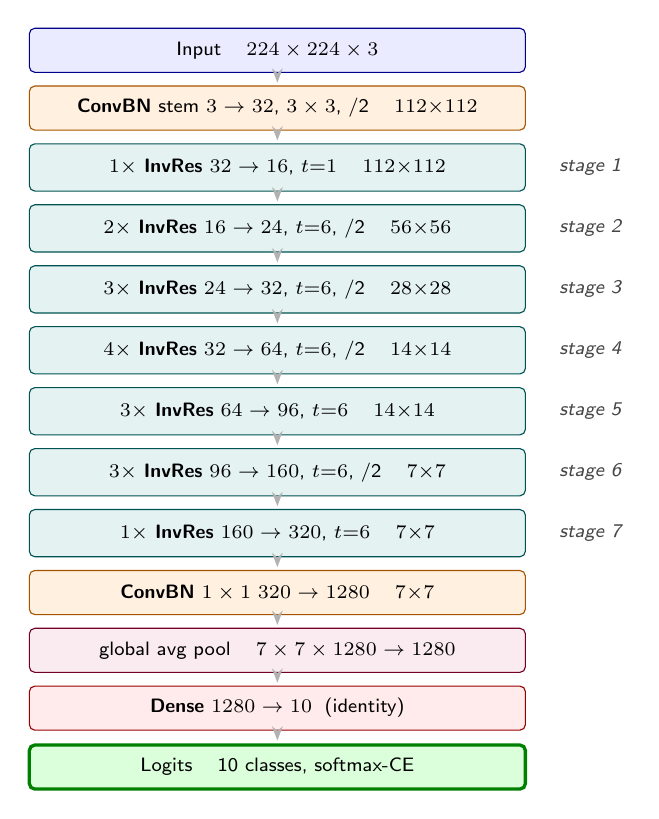
\begin{tikzpicture}[
  >={Stealth[length=1.8mm]},
  every node/.style={font=\sffamily\scriptsize},
  col/.style    = {align=center, rounded corners=2pt, inner sep=2pt, minimum height=0.56cm, minimum width=6.3cm},
  io/.style     = {col, draw=blue!55!black,   fill=blue!8},
  convbn/.style = {col, draw=orange!65!black, fill=orange!12},
  invres/.style = {col, draw=teal!65!black,   fill=teal!10, minimum height=0.6cm},
  gap/.style    = {col, draw=purple!60!black, fill=purple!8},
  head/.style   = {col, draw=red!60!black,    fill=red!8},
  logits/.style = {col, draw=green!50!black,  fill=green!14, very thick},
  arr/.style    = {->, thick, gray!60, shorten >=1pt, shorten <=1pt},
  stage/.style  = {font=\sffamily\scriptsize\itshape, gray!55!black, anchor=west},
]
  \node[io]                            (input) {Input \;\; $224\times224\times3$};
  \node[convbn, below=0.16cm of input] (stem) {\textbf{ConvBN} stem $3\to32$, $3\times3$, /2 \;\; $112{\times}112$};
  \node[invres, below=0.16cm of stem]  (s1)   {$1\times$ \textbf{InvRes} $32\to16$, $t{=}1$ \;\; $112{\times}112$};
  \node[invres, below=0.16cm of s1]    (s2)   {$2\times$ \textbf{InvRes} $16\to24$, $t{=}6$, /2 \;\; $56{\times}56$};
  \node[invres, below=0.16cm of s2]    (s3)   {$3\times$ \textbf{InvRes} $24\to32$, $t{=}6$, /2 \;\; $28{\times}28$};
  \node[invres, below=0.16cm of s3]    (s4)   {$4\times$ \textbf{InvRes} $32\to64$, $t{=}6$, /2 \;\; $14{\times}14$};
  \node[invres, below=0.16cm of s4]    (s5)   {$3\times$ \textbf{InvRes} $64\to96$, $t{=}6$ \;\; $14{\times}14$};
  \node[invres, below=0.16cm of s5]    (s6)   {$3\times$ \textbf{InvRes} $96\to160$, $t{=}6$, /2 \;\; $7{\times}7$};
  \node[invres, below=0.16cm of s6]    (s7)   {$1\times$ \textbf{InvRes} $160\to320$, $t{=}6$ \;\; $7{\times}7$};
  \node[convbn, below=0.16cm of s7]    (pw)   {\textbf{ConvBN} $1\times1$ $320\to1280$ \;\; $7{\times}7$};
  \node[gap,    below=0.16cm of pw]    (g)    {global avg pool \;\; $7\times7\times1280 \to 1280$};
  \node[head,   below=0.16cm of g]     (d)    {\textbf{Dense} $1280\to10$ \;(identity)};
  \node[logits, below=0.16cm of d]     (out)  {Logits \;\; 10 classes, softmax-CE};
  \foreach \a/\b in {input/stem, stem/s1, s1/s2, s2/s3, s3/s4, s4/s5, s5/s6,
                     s6/s7, s7/pw, pw/g, g/d, d/out}
     \draw[arr] (\a) -- (\b);
  \foreach \n/\k in {s1/1, s2/2, s3/3, s4/4, s5/5, s6/6, s7/7}
     \node[stage] at ($(\n.east) + (0.30,0)$) {stage \k};
\end{tikzpicture}

\vspace{0.45cm}

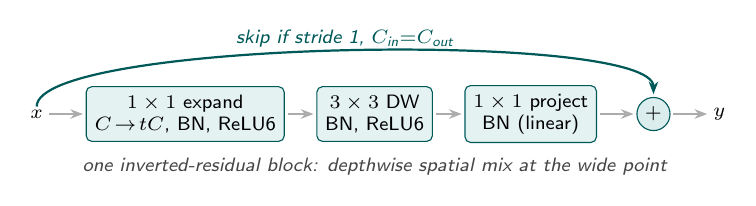
\begin{tikzpicture}[
  >={Stealth[length=1.6mm]},
  every node/.style={font=\sffamily\scriptsize},
  box/.style  = {align=center, rounded corners=2pt, inner sep=3pt, minimum height=0.62cm, draw=teal!70!black, fill=teal!10},
  dot/.style  = {circle, draw=teal!70!black, fill=teal!14, inner sep=0pt, minimum size=0.42cm},
  term/.style = {font=\sffamily\scriptsize\itshape, inner sep=1pt},
  arr/.style  = {->, thick, gray!65, shorten >=1pt, shorten <=1pt},
  skip/.style = {->, thick, teal!70!black, shorten >=1pt},
]
  \node[term]                       (x)   {$x$};
  \node[box, right=0.5cm of x]      (e)   {$1\times1$ expand\\$C\!\to\!tC$, BN, ReLU6};
  \node[box, right=0.4cm of e]      (dw)  {$3\times3$ DW\\BN, ReLU6};
  \node[box, right=0.4cm of dw]     (p)   {$1\times1$ project\\BN (linear)};
  \node[dot, right=0.5cm of p]      (sum) {$+$};
  \node[term, right=0.5cm of sum]   (y)   {$y$};
  \draw[arr] (x)  -- (e);
  \draw[arr] (e)  -- (dw);
  \draw[arr] (dw) -- (p);
  \draw[arr] (p)  -- (sum);
  \draw[arr] (sum) -- (y);
  \draw[skip] (x.north) .. controls +(0,0.85) and +(0,0.85) .. (sum.north)
        node[midway, above, term, teal!70!black] {skip if stride 1, $C_{\text{in}}{=}C_{\text{out}}$};
  \node[term, below=0.16cm of dw, gray!55!black] {one inverted-residual block: depthwise spatial mix at the wide point};
\end{tikzpicture}
\end{center}

\subsection*{The verified trainer}

\S\ref{sec:verified_trainer_pattern} is the pattern and this is the
first chapter to reuse it, so read the two together. Everything that
carries weight there carries the same weight here, and only the
\texttt{layers} list and the \texttt{bnChannels} that follows from it
are new:

\begin{verbatim}
import LeanMlir

-- 1. The network. `slug` names the committed render, `bnChannels`
--    drives BN threading, `NB` means the convs carry no bias.
def mobilenetv2Verified : VerifiedNetSpec where
  name     := "MobileNetV2"
  slug     := "mobilenetv2"
  inC      := 3
  imageH   := 224
  imageW   := 224
  nClasses := 10
  data     := .imagenette
  layers   := [
    .convBnNB 3 32 3 2,                   -- stem       224->112
    .invertedResidualNB  32   32  16 1,   -- stage 1, t=1   @112
    .invertedResidualNB  16   96  24 2,   -- stage 2    112->56
    .invertedResidualNB  24  144  24 1,
    .invertedResidualNB  24  144  32 2,   -- stage 3     56->28
    .invertedResidualNB  32  192  32 1,   --   x2
    .invertedResidualNB  32  192  64 2,   -- stage 4     28->14
    .invertedResidualNB  64  384  64 1,   --   x3
    .invertedResidualNB  64  384  96 1,   -- stage 5        @14
    .invertedResidualNB  96  576  96 1,   --   x2
    .invertedResidualNB  96  576 160 2,   -- stage 6      14->7
    .invertedResidualNB 160  960 160 1,   --   x2
    .invertedResidualNB 160  960 320 1,   -- stage 7         @7
    .convBnNB 320 1280 1 1,               -- head, 1x1 to 1280
    .globalAvgPool,
    .dense 1280 10 ]
  bnChannels := #[32, 32,16, 96,96,24, ... ]  -- all 52, in order

-- 2. The schedule. Identical to ResNet-34's, deliberately.
def mobilenetv2AdamConfig : VerifiedConfig where
  epochs    := 80
  batchSize := 32

-- 3. The entry point: AdamW, cosine with a 3-epoch warmup, baseLR 1e-3.
def main (argv : List String) : IO Unit :=
  mobilenetv2Verified.toNet.trainAdamSched
    mobilenetv2AdamConfig (argv.head?.getD "data") 0.001 0.9 0.999 3 "adam"
\end{verbatim}

\noindent Lines marked \texttt{x2} or \texttt{x3} appear that many times
in the source. The spec has no repeat count, because one constructor is
one block: \texttt{.invertedResidualNB ic mid oc stride} takes the
\emph{expanded} width \texttt{mid} rather than a ratio \(t\), so the
widths read straight off the paper's table and the stage boundaries are
visible as the places where \texttt{stride} is 2. Internally each block
is a $1 \times 1$ conv to \texttt{mid} channels, a $3 \times 3$
depthwise at that width, a $1 \times 1$ project to \texttt{oc}, and a
residual skip when \texttt{ic == oc} and \texttt{stride == 1}. Its VJP
is \S~\ref{ax:depthwise_has_vjp3} for the depthwise conv composed with
the dense, BN and biPath theorems already proved.

\textbf{Fifty-two BatchNorms, and the list is not three per block.} Every
inverted-residual block normalizes after each of its three convs, which
would be $17 \times 3 + 2$ for the stem and head, or 53. The first block
has expansion $t{=}1$, so it has no expand conv at all and contributes
two entries rather than three, and the real count is 52. That is the kind
of detail \texttt{bnChannels} exists to get right: the running-stat region
is positional, and an off-by-one there misaligns every frozen statistic
downstream of it at evaluation time.

\textbf{And the arm shows you the 52.} \texttt{.invertedResidualNB} is
one more entry on Chapter~\ref{chap:tensor}'s \texttt{toSpecs}, and the
$t{=}1$ carve-out above is not prose --- it is the conditional:

\begin{verbatim}
  | invertedResidualNB ic mid oc _ =>          -- Ch. 6
    (if mid != ic then #[(#[mid,ic,1,1],0),(#[mid],1),(#[mid],2)] else #[])
    ++ #[(#[mid,1,3,3],0),(#[mid],1),(#[mid],2),      -- depthwise 3x3 + BN
         (#[oc,mid,1,1],0),(#[oc],1),(#[oc],2)]       -- project 1x1 + BN
\end{verbatim}

\noindent \texttt{mid != ic} is exactly ``$t \neq 1$''. When it holds the
block contributes nine tensors and three BatchNorms; when it fails the
expand conv is not emitted at all and the block contributes six and two.
Sixteen blocks at three plus one at two, plus the stem and the head, is
the 52. The depthwise kernel is \texttt{[mid,1,3,3]} --- one filter per
channel, which is the whole of Theorem~\ref{ax:depthwise_has_vjp3}'s
subject written as a shape.

\textbf{The recipe is ResNet-34's, unchanged.} Eighty epochs at batch 32,
AdamW at $10^{-3}$, cosine with a three-epoch warmup, label smoothing
$0.1$, the same augmentation. That is on purpose. Holding the recipe fixed
is what makes the accuracy in \S\ref{sec:mnv2_runit} a comparison between
two \emph{architectures} rather than between two training setups, and it
is the same move Chapter~\ref{chap:bn} used to compare optimizers against
one proven gradient. MobileNetV2's own optimizer is RMSProp, which
\S\ref{sec:mnv2_imagenet} comes back to, and it is rendered at this shape
too: \texttt{LEAN\_MLIR\_VARIANT=rms} loads
\texttt{mobilenetv2\_rms\_train\_step.mlir} instead.

\subsection*{Results}

\S\ref{sec:mnv2_runit} has the run: 80 epochs at about 26
seconds each on one RTX 4060 Ti, finishing at \textbf{89.25\%}
top-1 and \textbf{98.68\%} top-5 on Imagenette's 3,925-image
validation split. Against Chapter~\ref{chap:residual}'s ResNet-34 at
$89.71\%$ on the same data and the same recipe, that is
\textbf{0.46 points of top-1} for \textbf{9.5$\times$ fewer parameters}
(2.24M against 21.3M). That is the depthwise-separable trade, and on
this evidence it is a better one than the architecture's reputation
suggests. Rather than reprint the log, here is what is worth noticing
in it.

- \textbf{2.24M parameters, and 1.05\,MB of MLIR} (1\,047\,327 chars)
  for the AdamW training step. ResNet-34 emitted 729\,KB with $9.5\times$
  the parameters, so the smaller network renders the \emph{larger}
  program. Emission is per-op, and the separable block trades one
  convolution for three, each with its own BatchNorm. Parameter count
  went down and operation count went up, and the text follows the
  second.

- \textbf{Per-step time is about 90\,ms} at batch 32, against
  ResNet-34's 220\,ms at the same batch and the same 295 steps to the
  epoch, so the whole run takes thirty-five minutes rather than an hour
  and a half. That is a real $2.4\times$, and it is also well short of
  what the parameter count promises: $9.5\times$ fewer weights buys
  $2.4\times$ the throughput, not $9.5\times$. Depthwise convolution is
  memory-bound. It does nine multiply-accumulates per output element
  where the standard $3 \times 3$ it replaces does $9 C_\text{in}$, so
  the kernel spends its time moving activations rather than multiplying
  them, and arithmetic was never the whole bottleneck.
  \S\ref{sec:mnv2_imagenet} sees the same sub-proportional scaling at
  ImageNet.

- \textbf{Three artifacts, not one.} The train step is accompanied by
  \texttt{mobilenetv2\_fwd} (143\,476 chars) and
  \texttt{mobilenetv2\_fwd\_eval} (111\,150 chars), the second existing
  only because BatchNorm evaluates differently than it trains. It is
  the concrete cost of the \texttt{bnChannels} line in the spec above.

- \textbf{52 BN layers}, up from ResNet-34's 36, for the same reason
  the MLIR is bigger: more internal convolutions means more
  BN-after-conv pairs. Each one still proves its VJP via
  \S~\ref{thm:bn_has_vjp}.

- \textbf{Final loss plateaus near 0.50} again, and for the same reason
  it did in Chapter~\ref{chap:residual}. The label-smoothing floor at
  $\varepsilon = 0.1$ over ten classes is about $0.485$, so this run has
  essentially converged rather than stalled.

\section{MLIR: Depthwise Convolution}

\noindent\textbf{What is already proven.} A depthwise convolution
applies one $k\times k$ kernel per channel with no cross-channel sum, so its
reverse-mode derivative (\S~\ref{ax:depthwise_has_vjp3},
\texttt{depthwise\_has\_vjp3}) is a reversed-kernel convolution \emph{minus}
the channel transpose the full-conv VJP of Chapter~\ref{chap:cnn} needs:
with no $\sum_{c_\text{in}}$ to take the adjoint of, there is no in/out
channel axis to swap. The inverted-residual block composes this with the
pointwise convs, BatchNorm, and relu6, and
\texttt{mobilenetv2\_full\_has\_vjp\_at} chains the whole network through
\texttt{vjp\_comp\_at}.

\medskip\noindent\textbf{The gap and how we close it.} The emitted graph
is denoted and shown equal to \texttt{depthwise\_has\_vjp3}'s backward. Here
is what the printer emits for the depthwise input gradient (two channels,
$3\times3$):

\begin{verbatim}
func.func @dw_back(%dy: tensor<1x2x4x4xf32>, %W: tensor<2x3x3xf32>)
    -> tensor<1x2x4x4xf32> {
  %We = stablehlo.reshape %W
          : (tensor<2x3x3xf32>) -> tensor<2x1x3x3xf32>
  %Wr = stablehlo.reverse %We, dims = [2, 3] : tensor<2x1x3x3xf32>
  %dx = stablehlo.convolution(%dy, %Wr)
      dim_numbers = [b, f, 0, 1]x[o, i, 0, 1]->[b, f, 0, 1],
      window = {stride = [1, 1], pad = [[1, 1], [1, 1]],
                lhs_dilate = [1, 1], rhs_dilate = [1, 1]}
      {batch_group_count = 1 : i64, feature_group_count = 2 : i64}
      : (tensor<1x2x4x4xf32>, tensor<2x1x3x3xf32>)
        -> tensor<1x2x4x4xf32>
  return %dx : tensor<1x2x4x4xf32>
}
\end{verbatim}

\noindent Read it against Chapter~\ref{chap:cnn}'s \texttt{conv\_back}. That
one began with a \texttt{transpose \%W, dims = [1, 0, 2, 3]} to swap the in-
and out-channel axes before reversing, and this one has \emph{no transpose}.
The \texttt{reshape} only adds the singleton input-channel axis the grouped
form expects ($[c,k,k] \to [c,1,k,k]$), the \texttt{reverse} flips the two
spatial axes, and \texttt{feature\_group\_count = 2}, equal to the channel
count, tells the convolution to run each channel through its own filter with
no mixing. That single attribute \emph{is} the depthwise structure, and the
bridge theorem is the claim that this graph computes
\texttt{depthwise\_has\_vjp3}'s backward.

\medskip\noindent\textbf{Caveats.}
\begin{itemize}
  \item \textbf{The depthwise convolution bridge is unconditional}, because
    it is linear.
  \item \textbf{relu6 is a smooth-point bridge.} MobileNetV2's clamp to
    $[0,6]$ has no derivative where a pre-activation sits exactly at $0$ or
    $6$, and the bridge may fail only on that measure-zero set.
  \item \textbf{Representative scale} (two channels at $4\times4$).
\end{itemize}

\section{ImageNet recipe}

\imagenettimmnote
\label{sec:mnv2_imagenet}

\imagenetphasenote

The Imagenette run above trained on $\sim$9.5K images. The same
backbone scales to full 1000-class ImageNet exactly the way
ResNet-34 did in Chapter~\ref{chap:residual}: the inverted-residual
stack is unchanged, only the head widens to 1000 and the dataset and
schedule grow. Everything in this section up to
\S\ref{sec:mnv2_phase4} was measured on the phase-2 (Lean$\to$JAX)
trainer, whose spec and recipe are:

\begin{verbatim}
-- Same inverted-residual backbone, 1000 classes instead of 10.
def mobilenetV2Imagenet : NetSpec where
  name   := "MobileNetV2 (ImageNet, bf16)"
  imageH := 224
  imageW := 224
  layers := [
    .convBn 3 32 3 2 .same,
    .invertedResidual  32  16 1 1 1,
    .invertedResidual  16  24 6 2 2,
    .invertedResidual  24  32 6 2 3,
    .invertedResidual  32  64 6 2 4,
    .invertedResidual  64  96 6 1 3,
    .invertedResidual  96 160 6 2 3,
    .invertedResidual 160 320 6 1 1,
    .convBn 320 1280 1 1 .same,
    .globalAvgPool,
    .dense 1280 1000 .identity      -- 1000-class head
  ]

-- RMSProp recipe, MobileNet-native: smaller weight decay, bf16 conv on.
def mobilenetV2ImagenetConfig : TrainConfig where
  learningRate   := 0.045           -- MobileNetV2-native RMSProp peak (was 0.1 for SGD)
  batchSize      := 256
  epochs         := 90              -- the real run; validate at 30 first
  optimizer      := .rmsprop        -- paper: RMSProp + momentum, not SGD
  momentum       := 0.9             -- mu for the RMSProp momentum buffer
  rmspropDecay   := 0.9             -- rho, the running mean-square decay
  rmspropEps     := 1.0             -- MobileNetV2 uses epsilon = 1.0
  weightDecay    := 4e-5            -- smaller than R34's 1e-4
  cosineDecay    := true
  warmupEpochs   := 5
  augment        := true            -- random-crop + horizontal flip
  useAutoAugment := false           -- MNv2 paper used crop/flip only, no AA
  labelSmoothing := 0.1
  bf16           := true
  bf16Conv       := true            -- reaches the inverted-residual blocks
\end{verbatim}

The one knob specific to MobileNet is \texttt{bf16Conv}. ResNet's
convolutions cast to bfloat16 the instant the flag is on, but
MobileNet's compute lives inside inverted-residual blocks (a
$1\times1$ expansion, a depthwise $3\times3$, a $1\times1$
projection) whose convolutions originally ran in fp32 regardless.
Routing them through the same \texttt{convdt} cast as the plain
convolutions is what lets bf16 reach the bulk of the network. The
payoff is the whole inverted-residual block running $\sim2\times$
faster on cuDNN, where the $1\times1$s (which are really matmuls)
love bfloat16 and the depthwise $3\times3$ is a wash. The weight
decay also drops to $4\times10^{-5}$, because MobileNet's depthwise
filters are tiny at nine weights per channel, and the $10^{-4}$ that
suits ResNet over-regularizes them.

\textbf{Compute budget.} On four RTX 4060 Ti (CUDA, bf16, batch 256),
steady-state throughput is about $6.6$ minutes per epoch, so the
paper's 350-epoch schedule takes roughly 45 wall-clock hours. The
wall-clock win over the $9.5\times$-larger ResNet-34 is real but
sub-proportional, exactly as \S\ref{sec:mnv2_runit} measured at small
scale: depthwise convolution is memory-bound and
low-arithmetic-intensity, so MobileNet's order-of-magnitude FLOP
saving buys a factor of two or three on this hardware rather than a
factor of nine.

\begin{center}
\begin{tabular}{l l r r r r r}
\hline
GPU & Precision & Per epoch & Epochs & Total & Val top-1 & Val top-5 \\
\hline
4$\times$ 4060 Ti (CUDA) & bf16 & $\sim$6.6 min & 350 (exp-decay) & $\sim$45 hr & $\mathbf{71.44\%}$ & $\mathbf{90.34\%}$ \\
\hline
\end{tabular}
\end{center}

\noindent The RMSProp peak LR of $0.045$ took off cleanly
with no collapse, because the large $\varepsilon=1.0$ keeps the
adaptive step well-damped (in sharp contrast to EfficientNet's
$\varepsilon=10^{-3}$ in Chapter~\ref{chap:se}, which is far more
LR-sensitive), so the $\sim$0.02 fallback was never needed.

\medskip\noindent Two evaluations get reported for a run like this and
they are not the same measurement, so it is worth saying which is which
once. The \emph{curve} below is the in-loop evaluation the trainer runs
at the end of an epoch, on the 49{,}920 validation images that survive
batching, using the live weights. The \emph{headline} is an offline pass
over the full 50{,}000 images using the EMA weights. The second is the
number to quote against a paper, and the first is the one to read for
shape.

\subsection*{The paper-faithful tier: 350 epochs}

The recipe above is the paper's, and the schedule is the part of it that
is easiest to get wrong. Sandler et al.\ use no label smoothing, an
exponential decay of $\times0.98$ per epoch, and on the order of 350
epochs, and those three go together rather than being independently
adjustable. Shortening the schedule forces the other two.

The reason is that under
$\times 0.98$/epoch the learning rate after $90$ epochs is still
$0.045 \times 0.98^{85} \approx 8.1\times10^{-3}$, barely annealed,
with none of the end-of-schedule polish a cosine run has already
collected by then. Only over $350$ epochs does the exponential reach
$0.045 \times 0.98^{345} \approx 4.2\times10^{-5}$ and behave as
intended. So a shortened run of this recipe has to substitute cosine to
be worth anything at all, which is a different experiment rather than a
cheaper version of the same one.

Run end to end on four 4060 Ti it lands at $\mathbf{71.44\%}$ top-1
and $\mathbf{90.34\%}$ top-5 on the full 50{,}000-image validation
split, $\mathbf{0.56}$ points short of the paper's $72.0\%$:

\begin{center}
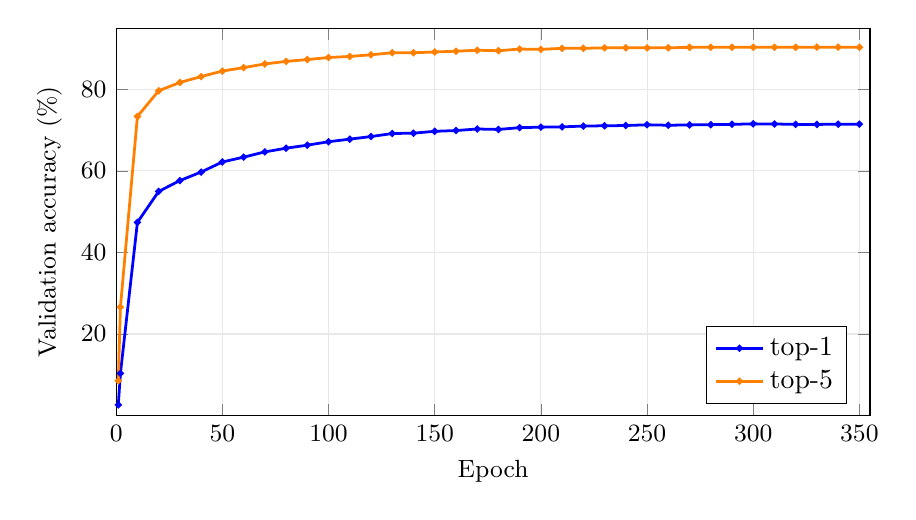
\begin{tikzpicture}
\begin{axis}[
    width=0.92\linewidth, height=6.5cm,
    xlabel={Epoch}, ylabel={Validation accuracy (\%)},
    xmin=0, xmax=355, ymin=0, ymax=95,
    xtick={0,50,100,150,200,250,300,350}, ytick={20,40,60,80},
    legend pos=south east, legend cell align={left},
    grid=major, grid style={gray!18},
    tick label style={font=\small}, label style={font=\small},
    every axis plot/.append style={line width=1pt, mark size=0.7pt},
]
\addplot[blue, mark=*, mark options={fill=blue}] coordinates {
(1,2.60) (2,10.34) (10,47.38) (20,54.96) (30,57.63) (40,59.72) (50,62.19) (60,63.37) (70,64.66) (80,65.57) (90,66.31) (100,67.16) (110,67.79) (120,68.43) (130,69.17) (140,69.26) (150,69.71) (160,69.90) (170,70.28) (180,70.17) (190,70.61) (200,70.73) (210,70.80) (220,71.00) (230,71.07) (240,71.13) (250,71.31) (260,71.20) (270,71.28) (280,71.35) (290,71.42) (300,71.54) (310,71.51) (320,71.41) (330,71.40) (340,71.46) (350,71.46)
};
\addlegendentry{top-1}
\addplot[orange, mark=*, mark options={fill=orange}] coordinates {
(1,8.53) (2,26.58) (10,73.36) (20,79.66) (30,81.69) (40,83.14) (50,84.49) (60,85.33) (70,86.24) (80,86.86) (90,87.31) (100,87.81) (110,88.08) (120,88.48) (130,88.99) (140,88.98) (150,89.17) (160,89.36) (170,89.60) (180,89.48) (190,89.89) (200,89.82) (210,90.06) (220,90.08) (230,90.19) (240,90.20) (250,90.18) (260,90.19) (270,90.31) (280,90.31) (290,90.31) (300,90.33) (310,90.33) (320,90.31) (330,90.36) (340,90.35) (350,90.33)
};
\addlegendentry{top-5}
\end{axis}
\end{tikzpicture}
\end{center}

\noindent MobileNetV2 / ImageNet-1k, paper-faithful 350-epoch
exponential-decay run (bf16, 4$\times$ 4060 Ti, RMSProp).

Two thirds of the final accuracy is in place by epoch $50$, the run is
still climbing at $150$, and it is flat from about epoch $250$ onward, so
the last $100$ epochs are worth almost nothing and the schedule is
genuinely exhausted rather than cut short.

That residual $0.56$ is provisional rather than explained, and the marker
at the top of this section is why: these numbers predate \texttt{timm}'s
validation protocol and its antialiased resampler, and that change moves
the training distribution as well as the evaluation
(appendix~\ref{app:data}). Two known deviations are the candidates, both
shared across every net in this book --- the resize is not antialiased on
either the train or eval path where timm's is, and the running-BN decay is
fixed at $0.99$ where PyTorch's default works out to $0.9$. No points are
attributed to either one here, because the first is precisely what the
re-run changes, and a split quoted now would be a split of a number the
re-run replaces.

\subsection*{Phase 4: the verified trainer}
\label{sec:mnv2_phase4}

Everything above this point is the phase-2 Lean$\to$JAX trainer. The
phase-4 peer, which trains the same network through the proof-rendered
StableHLO that \S\ref{sec:mnv2_runit} ran at Imagenette scale, exists and
builds. It is
\texttt{apps/imagenette/MainMobileNetV2Imagenet.lean}, built as
\texttt{lake build mobilenetv2-imagenet-verified}:

\begin{verbatim}
-- Same inverted-residual backbone, 1000 classes instead of 10.
def mobilenetv2ImagenetVerified : VerifiedNetSpec where
  name       := "MobileNetV2 (ImageNet-1k)"
  slug       := "mobilenetv2in"
  nClasses   := 1000
  data       := .imagenet
  shimScript := "generated_mobilenet_v2_imagenet_shim.py"
  layers     := [ ... the Imagenette stack, 1000-class head ... ]

-- 350 epochs at 64 PER DEVICE; four replicas give the global 256.
-- 350 because that is the schedule the phase-2 number above was measured on.
def mobilenetv2ImagenetConfig : VerifiedConfig where
  epochs    := 350
  batchSize := 64

def main (argv : List String) : IO Unit :=
  mobilenetv2ImagenetVerified.toNet.trainAdamSched
    mobilenetv2ImagenetConfig (argv.head?.getD "data") ... variant
\end{verbatim}

\noindent \texttt{slug} names
\texttt{verified\_mlir/mobilenetv2in\_<variant>\_train\_step.mlir}, the
rendered graph, and \texttt{shimScript} names this net's own augmentation
shim rather than ResNet-34's, both for the reasons
\S\ref{sec:r34_phase4} gives. The head is the only parameter shape that
moves, from $1280 \times 10$ to $1280 \times 1000$, which takes the count
from 2.24M to \textbf{3,504,872} and matches the JAX reference exactly.
The BatchNorm layout is required to be byte-identical to the Imagenette
net's, and a \texttt{\#guard} enforces it, because the running-stat region
is positional and a drift there would misalign every frozen statistic at
evaluation.

\textbf{The variant selects the optimizer, and one of them is the
paper's.} At \texttt{rms64} the driver loads
\texttt{mobilenetv2in\_rms64\_train\_step.mlir}, which has the recipe
tabulated below rendered into it: RMSProp at $\rho = 0.9$, $\mu = 0.9$,
$\varepsilon = 1.0$ and coupled weight decay $4 \times 10^{-5}$, at peak
LR $0.045$ with a 5-epoch warmup and $\times 0.98$ per epoch after it.
Those constants live in \texttt{mnv2RmsSchedule} and
\texttt{mnv2RmsHyper}, shared with the Imagenette peer so the two cannot
carry different values. At \texttt{adam64} it is AdamW at $10^{-3}$
instead, which is the default because it matches the other four
ImageNet drivers.

\medskip\noindent\textbf{The schedule is 350 epochs because the run it
has to match is.} The point of a phase-4 run is not to train this network
once, it is to reproduce the phase-2 result on the verified path, and the
phase-2 result above is the paper-faithful 350-epoch exponential-decay
tier at $71.44\%$. A 300-epoch phase-4 run would not answer that
question. \texttt{totalSteps} is what the schedule anneals over, so 300
against 350 is a different learning-rate curve end to end rather than a
shorter version of the same one, and the two numbers would not be
comparable.

\medskip\noindent\textbf{What it has not done is run.} No phase-4
ImageNet result exists for this network, which is why every accuracy
above comes from phase 2. What is measured is the throughput, and the
schedule follows from it:

\begin{center}
\begin{tabular}{l r r r r}
\hline
Box & ms/step & min/epoch & 350 epochs & Val top-1 \\
\hline
4$\times$ 4060 Ti (CUDA)  & 129 & 10.8 & $\sim$66.4 h (2.8 d) & TBD \\
4$\times$ 3060 (CUDA)     &  99 &  8.3 & $\sim$51.8 h (2.2 d) & TBD \\
2$\times$ 7900 XTX (ROCm) & --- & ---  & ---                  & TBD \\
\hline
\end{tabular}
\end{center}

\noindent\textbf{[TODO: run \texttt{mobilenetv2-imagenet-verified}.]}

\subsection*{What the MobileNetV2 recipe changes from the 2018 recipe}

The ResNet-34 trainer of Chapter~\ref{chap:residual} is the
\emph{2018-era} recipe of the SGD lineage: momentum, cosine polish,
label smoothing. MobileNetV2 is a 2018 paper too, but from the other
side of a fork. Google's TensorFlow and Inception training tradition
runs RMSProp with a huge $\varepsilon$, an exponential LR staircase, a
tiny weight decay, and nothing beyond crop and flip on the data
side. So this diff is not a time jump but two contemporary recipes
side by side, and it is the base that the next chapter's 2019
EfficientNet recipe is built on. The entry point is the same on both
paths, and every row below is one argument or one field:

\begin{center}
\begin{tabular}{@{}l p{2.9cm} p{3.2cm} p{6.3cm}@{}}
\hline
Knob & ResNet-34 (2018) & MobileNetV2 (2018) & What the MNv2 choice buys \\
\hline
Backbone      & basic block, 21.8\,M   & inverted residual, 3.5\,M     & depthwise $3\times3$ at the wide point between $1\times1$s, at $1/6$ the parameters \\
Optimizer     & SGD + momentum $0.9$   & RMSProp                       & $\rho{=}0.9$, $\mu{=}0.9$, $\varepsilon{=}1.0$, where the huge $\varepsilon$ keeps the adaptive step damped (B0 shrinks it to $10^{-3}$ and pays for it) \\
Peak LR       & $0.1$                  & $0.045$                       & RMSProp's scale, not comparable to SGD's $0.1$ \\
LR schedule   & cosine to zero         & exponential, $\times0.98$ per epoch & the TF-lineage staircase the whole family inherits \\
Epochs        & 90                     & $\sim$300--400                & the long-haul schedule, and the row the exponential decay above makes non-negotiable \\
Weight decay  & $10^{-4}$, all params  & $4\times10^{-5}$              & depthwise filters are 9 weights per channel, and $10^{-4}$ over-regularizes them \\
Label smoothing & $0.1$                & none                          & Sandler et al.\ used no smoothing at all \\
Augmentation  & RRC + hflip            & RRC + hflip                   & unchanged, with no learned policy and no mixing, the leanest recipe in this book \\
\hline
\end{tabular}
\end{center}

\noindent What carries over unchanged: batch 256, train and eval both
at $224$, running-BN evaluation, bf16 matmul and convolution, and our
5-epoch warmup (an addition to both papers).

The through-line of this fork is that nothing here regularizes harder.
MobileNetV2's recipe is the SGD recipe's contemporary, tuned for a
network $1/6$ the size, and its distinctive knobs (adaptive
optimizer, staircase decay, tiny selective-in-spirit weight decay)
are the ones EfficientNet inherits and ConvNeXt eventually replaces
wholesale. The 2019--2022 tables that follow all diff against the
same 2018 SGD column. This one shows where their other half came
from.

The general pattern is deeper and narrower, with a per-channel conv
between surrounding $1 \times 1$ expansions, and it carries forward to
MobileNet V3 and the EfficientNet family. All of those add their own
small modifications on top (SE blocks, Swish activations, compound
scaling) but the core depthwise-separable scaffolding is exactly what
this chapter formalized.

\section{Side quest: MobileNet V4}
\label{sec:mnv4_side_quest}

\imagenettimmnote

\imagenetphasenote

Six years on, MobileNetV4 (Qin et al.\ 2024,
\href{https://arxiv.org/abs/2404.10518}{arXiv:2404.10518}) revisits
this chapter's block. Its central move is the \emph{universal
inverted bottleneck} (UIB): take the inverted residual and make two
depthwise positions optional, one before the expansion and one after
it. Four instantiations fall out of that one template. Both
depthwise convs on is \emph{ExtraDW}. Only the leading one is
\emph{ConvNeXt}, this chapter's sandwich rearranged into
Chapter~\ref{chap:layernorm}'s block shape. Neither is a plain
\emph{FFN} of two $1\times1$s. Only the inner one is exactly
MobileNetV2's block. The \texttt{jax/} folder ships the faithful
Conv-Medium as a full ImageNet trainer
(\texttt{jax/MainMobilenetV4Imagenet.lean}), transcribed block for
block from timm's \texttt{mobilenetv4\_conv\_medium}: $\sim$9.7M
parameters, a fused-IB stage at high resolution, then 21 UIB blocks
whose per-block instantiation is visible right in the
\texttt{NetSpec}, driven by the same entry point as every other net
in this book. What changed from 2018 to 2024 is at
least as much recipe as architecture:

\begin{center}
\begin{tabular}{@{}l p{2.9cm} p{3.2cm} p{6.3cm}@{}}
\hline
Knob & MobileNetV2 (2018) & MNv4-Conv-M (2024) & What the v4 choice buys \\
\hline
Block         & inverted residual      & UIB (+ fused IB stage)        & the two optional depthwise slots subsume MNv2's block, ConvNeXt's, and an FFN in one template \\
Parameters    & 3.5\,M                 & 9.7\,M                        & ``mobile'' now means fits-the-phone, not smallest-possible \\
Paper top-1   & $72.0\%$               & $79.9\%$                      & non-distilled, and distillation pushes the family higher still \\
Optimizer     & RMSProp ($\varepsilon{=}1.0$) & AdamW $\beta(0.9, 0.999)$ & the TF-lineage staircase gives way to the transformer-era default \\
Peak LR       & $0.045$ @ 256          & $0.004$ @ 4096                & effective batch 4096 (run here as $512 \times 8$ grad-accum) \\
LR schedule   & exponential, $\times0.98$ per epoch & cosine, 5-epoch warmup & the anneal every post-2020 recipe in this book uses \\
Epochs        & $\sim$300--400         & 500                           & the family's long-haul habit, taken further \\
Weight decay  & $4\times10^{-5}$       & $0.1$, skip norm/bias         & $2500\times$ stronger, applied selectively, because AdamW makes heavy decay usable \\
Augmentation  & RRC + hflip            & + RandAugment (N2, m15, p0.7) & heavy learned augmentation, and still no Mixup/CutMix for Conv-M \\
Label smoothing & none                 & $0.1$                         & standard by 2024 \\
Stochastic depth & none                & drop-path $0.075$             & linear ramp over the 21 UIB blocks \\
EMA           & none                   & decay $0.9999$, warmup-corrected & weight averaging (with the BN buffers shadowed, per Ch~\ref{chap:se}'s lesson) \\
\hline
\end{tabular}
\end{center}

\noindent The direction of travel matches the recipe tables closing
Chapters~\ref{chap:se} and~\ref{chap:layernorm}: by 2024 the mobile
lineage has converged on the same transformer-era training
recipe as everything else (AdamW at large effective batch,
cosine, heavy selective decay, RandAugment, EMA) while the block
template generalized enough to absorb its rivals.

\textbf{One trap in that EMA row.} Seeding the shadow at the
initialization and decaying it away leaves $d^{\,t}$ of that
initialization behind. A random network and a trained one are not
joined by a low-loss path, so even a few percent of it puts the
average at \emph{chance} rather than merely behind. Conv-M trips this
where longer runs do not, because gradient accumulation leaves it only
$312$ steps per epoch, so $31{,}200$ total against a time constant of
$10{,}000$. The fix is TensorFlow's, which this family's reference
implementations assume: ramp the decay,
$d_t = \min\!\big(d,\ (1+t)/(10+t)\big)$.

\texttt{mobilenet-v4-imagenet} ships two tiers. \textbf{100 epochs}
(recipe \texttt{default}) is a reduced-regularization confidence
tier at wd $0.05$, dropout $0.1$ and RandAugment m9, since the paper's
full pack underfits short schedules. \textbf{500 epochs}
(recipe \texttt{full}) is the paper recipe end to end. The
100-epoch tier is the one run here, and the $79.9\%$ headline is a
500-epoch number:

\begin{center}
\begin{tabular}{l l r r r r r}
\hline
GPU & Precision & Per epoch & Epochs & Total & Val top-1 & Val top-5 \\
\hline
4$\times$ 4060 Ti (CUDA) & bf16 & $\sim$9.0 min & 100 (reduced-reg) & $\sim$16 hr & $\mathbf{75.48\%}$ & $\mathbf{92.37\%}$ \\
4$\times$ 4060 Ti (CUDA) & bf16 & $\sim$9.0 min & 500 (paper) & $\sim$75 hr & --- & --- \\
\hline
\end{tabular}
\end{center}

\noindent The 100-epoch tier lands at $\mathbf{75.48\%}$ top-1 and
$\mathbf{92.37\%}$ top-5 on the full 50{,}000-image validation split
(EMA weights). Set against this chapter's other half that is the
whole six-year argument in two rows: $\mathbf{+4.04}$ points over
MobileNetV2's paper-faithful $71.44\%$, from $2.8\times$ the
parameters and \emph{less than half} the epochs, $100$ against
$350$ and $16$ wall-clock hours against $45$.
By 2024 the mobile line is not trading accuracy for size so
much as reaching the same accuracy with a block that happens to be
cheap.

\begin{center}
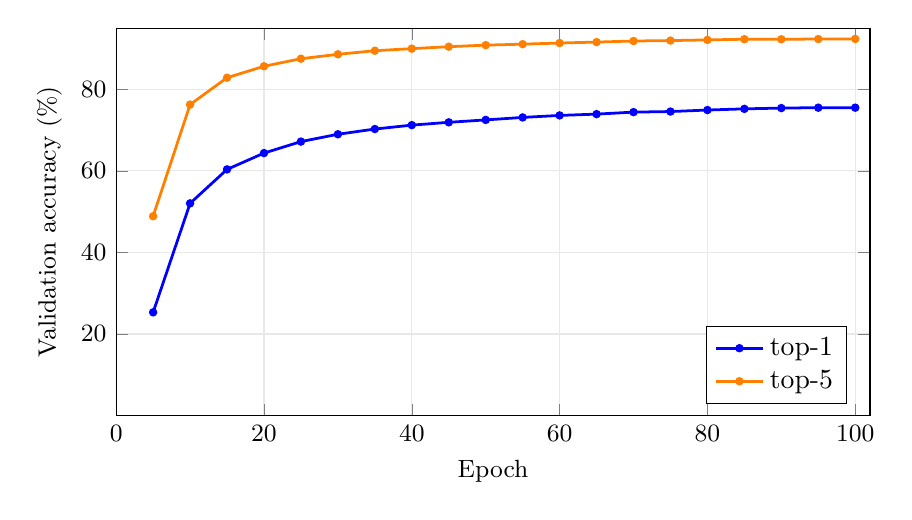
\begin{tikzpicture}
\begin{axis}[
    width=0.92\linewidth, height=6.5cm,
    xlabel={Epoch}, ylabel={Validation accuracy (\%)},
    xmin=0, xmax=102, ymin=0, ymax=95,
    xtick={0,20,40,60,80,100}, ytick={20,40,60,80},
    legend pos=south east, legend cell align={left},
    grid=major, grid style={gray!18},
    tick label style={font=\small}, label style={font=\small},
    every axis plot/.append style={line width=1pt, mark size=1pt},
]
\addplot[blue, mark=*, mark options={fill=blue}] coordinates {
(5,25.31) (10,52.04) (15,60.37) (20,64.37) (25,67.19) (30,68.99) (35,70.27) (40,71.23) (45,71.92) (50,72.51) (55,73.12) (60,73.61) (65,73.93) (70,74.42) (75,74.56) (80,74.93) (85,75.22) (90,75.41) (95,75.51) (100,75.51)
};
\addlegendentry{top-1}
\addplot[orange, mark=*, mark options={fill=orange}] coordinates {
(5,48.88) (10,76.27) (15,82.86) (20,85.67) (25,87.52) (30,88.60) (35,89.48) (40,89.99) (45,90.47) (50,90.85) (55,91.09) (60,91.37) (65,91.60) (70,91.86) (75,91.97) (80,92.13) (85,92.30) (90,92.29) (95,92.35) (100,92.37)
};
\addlegendentry{top-5}
\end{axis}
\end{tikzpicture}
\end{center}

\noindent MobileNetV4-Conv-M / ImageNet-1k, 100-epoch
reduced-regularization tier (bf16, 4$\times$ 4060 Ti, AdamW,
effective batch $4096$ via $512\times8$ gradient accumulation).

\textbf{[TODO, 500 epochs.]} \texttt{mobilenet-v4-imagenet full}.
The tier above is \emph{detuned} by construction, at wd $0.05$ against
the paper's $0.1$, dropout $0.1$ against $0.2$, and RandAugment $m9$
against $m15$, so its $75.48\%$ is not a reproduction of
$79.9\%$. Its in-loop curve is flat over the last ten epochs
($75.41 \to 75.51 \to 75.51$). The schedule is exhausted, and the
remaining points live in the regularization the \texttt{full} tier
restores.

\subsection*{Phase 4: MobileNetV4 on the verified path}
\label{sec:mnv4_phase4}

Everything above in this side quest is the phase-2 Lean$\to$JAX trainer
running the faithful Conv-Medium. The phase-4 peer exists as of this
writing, and it renders the same network.

The spec is built the way \S\ref{sec:mnv2_phase4} built MobileNetV2's
and the way Chapter~\ref{chap:residual} built ResNet-50's. The trunk is
copied unchanged from the Imagenette spec, a \texttt{\#guard} pins every
parameter shape but the head against it, and the head moves
$1280{\times}10 \to 1280{\times}1000$, taking the count from
$8{,}447{,}322$ to $\mathbf{9{,}715{,}512}$, which is the $\sim$9.7M
Conv-M is quoted at.

\textbf{The $75.48\%$ above is this network's target.} It is not
this network's result. The row below reports a measured wall clock and a
\texttt{TBD} accuracy, because the network has been timed and has not
been trained to convergence.

\begin{verbatim}
def mnv4ImagenetVerified : VerifiedNetSpec where
  name       := "MobileNetV4-Conv-M (ImageNet-1k)"
  slug       := "mnv4in"
  nClasses   := 1000
  data       := .imagenet
  shimScript := "generated_mobilenet_v4_imagenet_shim.py"
  layers     := [ ... the Imagenette UIB stack, 1000-class head ... ]

def main (argv : List String) : IO Unit :=
  mnv4ImagenetVerified.toNet.trainAdamSched
    { mnv4ImagenetConfig with batchSize := bs, epochs := epochs }
    (argv.head?.getD "data") baseLR 0.9 0.999 5 variant
\end{verbatim}

\noindent That is \texttt{apps/imagenette/MainMobilenetV4Imagenet.lean}.
It builds as \texttt{mobilenetv4-imagenet-verified}. The renders come
from the same chain and the same block table as the three 10-class
artifacts, differing only in \texttt{nClasses}, the batch and the slug,
which is why adding them was three \texttt{\#eval} lines rather than a
new proof chain.

\textbf{It runs.} All three artifacts compile under PJRT, the shim feeds
it, and a first step lands at loss $6.99$ against $\ln 1000 = 6.91$,
with evaluation at $0.106\%$ top-1 over the 49{,}920-image validation
split, which is $1/1000$ to two figures. Those are the numbers a
correctly wired 1000-class network produces before it has learned
anything, and they are the whole of what has been measured about its
accuracy so far.

\begin{center}
\begin{tabular}{l r r l r r}
\hline
Box & ms/step & min/epoch & Epochs & Total & Val top-1 \\
\hline
4$\times$ 4060 Ti (CUDA), global 256 & 126 & 10.5 & 100 (reduced-reg) & 18.6 h (0.8 d) & TBD \\
4$\times$ 4060 Ti (CUDA), global 256 & 126 & 10.5 & 500 (paper)       & 92.8 h (3.9 d) & TBD \\
4$\times$ 3060 (CUDA), global 256    & 109 &  9.1 & 100 (reduced-reg) & 16.2 h (0.7 d) & TBD \\
4$\times$ 3060 (CUDA), global 256    & 109 &  9.1 & 500 (paper)       & 81.0 h (3.4 d) & TBD \\
\hline
\end{tabular}
\end{center}

\noindent {\small Measured bf16 with the four-replica probe, as a median
over steady-state steps. Both four-replica renders are in the tree ---
\texttt{mnv4in\_adamdp64\_train\_step} and its \texttt{bf16} arm --- so
the artifact these numbers were taken on is one the reader can rebuild.
\textbf{And as of 2026-08-27 they are tied}, which is what this row used
to say was missing: MobileNetV4 now has a \texttt{shard-check} peer and a
duplicated-batch \texttt{mnv4-dp-check}, both green and both red against a
sum-not-mean control. So a schedule costed here can now also be run ---
\texttt{scripts/supervise.sh mnv4-default-4gpu}.}

\medskip\noindent Most of the four-card overhead here is not all-reduce.
At global 256 the host feeds four times as many images per step, and that
cost grows with the batch rather than with the model. The evidence is that
an estimate built the other way --- scaling MobileNetV2's measured
all-reduce cost by Conv-M's $2.77\times$ larger gradients --- missed the
measured figure by $70\%$.

\medskip\noindent\textbf{[TODO: run \texttt{mnv4-default-4gpu}.]} The job
config exists and its prechecks pass. Note that it ships the \emph{fp32}
arm by default --- $177$ ms/step, $\sim$$25.6$ hr --- where the rows above
are bf16; one line in the config switches it, and the choice was to move one
axis at a time rather than pair a first run with a precision change. The
\texttt{Val top-1} column stays \texttt{TBD} either way.

\chapter{EfficientNet}
\label{chap:se}

\prosesection{A convolution treats every channel equally}

By the time a feature map reaches a deep stage of a CNN, each
channel is a learned ``feature detector'' for something specific: a
headlight, a curve, a fur texture, a leaf edge. A standard
\(3 \times 3\) convolution that consumes this feature map treats
every one of those channels as equally important contributors to
every output channel. Its kernel learns a fixed mixing recipe
that's applied to every spatial position of every input image,
regardless of what's actually in the image.

That's wasteful in a particular way. A ``headlight'' channel is
useful when there's a car in the image and useless on a beach. A
``leaf-edge'' channel is useful in a tree-heavy region and useless
in the sky. The network has no built-in way to say ``for this
image, dial channel 47 up and channel 112 down.'' Hu et al.\ 2018
(\href{https://arxiv.org/abs/1709.01507}{arXiv:1709.01507})
designed a tiny module that lets the network do exactly that:
look at the global content of the feature map, produce a
per-channel gain, and rescale every channel by its gain before
passing the feature map forward.

That module is the \textbf{Squeeze-and-Excitation block}, and at
its core it is a learned per-channel attention mechanism that
predates the transformer-era ``attention'' by four years and
informs every post-2018 vision architecture.

\section{Run it first}
\label{sec:enet_runit}

Before the attention mechanism, train the network that uses it. Four
commands, and less GPU time than either of the two previous chapters:

\begin{verbatim}
lake exe cache get                            # Mathlib oleans, ~30 s
./download_imagenette.sh                      # 330 MB dl, 2.4 GB unpacked
lake build efficientnet-verified-adam
./.lake/build/bin/efficientnet-verified-adam data
\end{verbatim}

On one RTX 4060 Ti (CUDA 12.9), from
\texttt{runs/2026-08-12-enet-imagenette-xla-cuda/}. XLA's startup banner
is removed, the network description line is wrapped, and the middle of
the run is elided:

\begin{verbatim}
[pjrt_ffi] XLA backend: PJRT 0.112, 1 device(s)
[pjrt_ffi] compiled verified_mlir/efficientnet_adam_train_step.mlir
             (@efficientnet_adam_train_step, 740 outputs, 1 replica)
             in 10603 ms
[pjrt_ffi] compiled verified_mlir/efficientnet_fwd.mlir
             (@efficientnet_fwd, 1 outputs, 1 replica) in 635 ms
[pjrt_ffi] compiled verified_mlir/efficientnet_fwd_eval.mlir
             (@efficientnet_fwd_eval, 1 outputs, 1 replica) in 454 ms
EfficientNet-B0 on Imagenette 224² (stem-s2 → 16 MBConv [t,c,n,s,k],
  swish + squeeze-excite + batch-norm, 5 downsamples 224→7 →
  head 320→1280 → GAP → dense)
  via the VERIFIED renderer → XLA/PJRT → GPU
  train 9469, val 3925; bs 32, EfficientNet-B0 adam
    (cosine+warmup 3ep, baseLR 0.001000), He init
  running-stats BN: 49 layers, 42016 stat floats
    → eval via @efficientnet_fwd_eval
Epoch 1/80: loss=2.048415 lr=0.000333
  epoch 1: val_acc = 698/3925 = 17.783439%  top5 = 2753/3925 = 70.140127%
Epoch 2/80: loss=1.633202 lr=0.000667
  epoch 2: val_acc = 1356/3925 = 34.547771%  top5 = 2831/3925 = 72.127389%
Epoch 3/80: loss=1.421186 lr=0.001000
  epoch 3: val_acc = 1529/3925 = 38.955414%  top5 = 3113/3925 = 79.312102%
Epoch 4/80: loss=1.281925 lr=0.001000
  epoch 4: val_acc = 2520/3925 = 64.203822%  top5 = 3667/3925 = 93.426752%
Epoch 79/80: loss=0.504021 lr=0.000000
  epoch 79: val_acc = 3535/3925 = 90.063694%  top5 = 3865/3925 = 98.471338%
Epoch 80/80: loss=0.504361 lr=0.000000
  epoch 80: val_acc = 3531/3925 = 89.961783%  top5 = 3864/3925 = 98.445860%
done (trained EfficientNet-B0 adam + cosine/warmup via packed threading).
\end{verbatim}

Eighty epochs at about 30 seconds each, forty and a half minutes in
total, and \textbf{89.96\%} top-1 with \textbf{98.45\%} top-5 on
Imagenette's 3,925-image validation split. The best epoch reached
$90.14\%$. That is the highest top-1 in this book's Imagenette column:
ResNet-34 finished at $89.71\%$ and MobileNetV2 at $89.25\%$ on the same
data, the same recipe and the same eighty epochs. EfficientNet-B0 does it
with $5.3\times$ fewer parameters than ResNet-34 and in less than half
the wall-clock.

The first four epochs are worth a glance. Top-1 climbs 17.8, 34.5, 39.0,
then jumps to 64.2. The learning rate is still warming up through epoch
3, and the BatchNorm running statistics are averaging over weights that
are moving fast, so the evaluation forward is using statistics that no
longer describe what is being evaluated. It resolves once the schedule
reaches its peak and never recurs.

Squeeze-excitation is the first place the product rule carries real
weight. That run did not execute a
reimplementation of the network this chapter describes. It executed
\texttt{verified\_mlir/efficientnet\_adam\_train\_step.mlir}, which is
\texttt{pretty(provenGraph)} off the renderer. Every squeeze-excitation
gate in it backpropagates by the product rule
Theorem~\ref{thm:seBlock_has_vjp} proves, every depthwise convolution by
Chapter~\ref{chap:depthwise}'s, every BatchNorm by
Chapter~\ref{chap:bn}'s, and every residual skip by
Chapter~\ref{chap:residual}'s additive fan-in.

\medskip\noindent\textbf{And this fold holds at every input.}
\texttt{efficientnetForwardB\_full\_has\_vjp} chains the stem, all
\emph{sixteen} MBConv blocks and the head through \texttt{vjp\_comp},
batched over \(N\), assuming a positive \(\varepsilon\) at each BatchNorm
and nothing else --- so every operation in the graph that just trained
carries a proved backward, and their composition into the whole network
carries one too. What buys that is swish. It is smooth, so the statement
quantifies over all inputs, where Chapter~\ref{chap:depthwise}'s fold had
to name a point and assume its thirty-five relu6 activations stayed off
the kink. Depth was never the obstacle, the activation was --- and every
network after this one is smooth.

The three compile lines are the same three the two previous chapters
showed. \texttt{@efficientnet\_fwd\_eval} is a separate forward because
BatchNorm evaluates differently than it trains, and
\texttt{running-stats BN: 49 layers, 42016 stat floats} is the driver
threading the running averages out of the train step and into it. The
train step reports 740 outputs, which is what 213 parameter tensors plus
their Adam moments plus the batch statistics plus the report-only loss
come to.

To run this net alongside the other six at the same scale and recipe, see
\S\ref{sec:enet_imagenet} for what changes at ImageNet scale.

\prosesection{Three steps, one tensor product}

An SE block on a feature map \(x \in \mathbb{R}^{B \times C \times H \times W}\)
runs three operations in sequence:

\begin{enumerate}
\item \textbf{Squeeze.} Global-average-pool across spatial
  dimensions: \(s_c = \frac{1}{HW} \sum_{i,j} x_{c, i, j}\). Result
  is a \(B \times C\) tensor: one scalar per image per channel,
  summarizing the channel's overall activity.

\item \textbf{Excite.} Push \(s\) through a tiny two-layer MLP with
  a bottleneck:
  \(g = \sigma(W_2\, \mathrm{ReLU}(W_1 s))\), where \(W_1\) is
  \(C \to C/r\) and \(W_2\) is \(C/r \to C\) for a reduction ratio
  \(r\) (typically 16). The sigmoid squashes each output to
  \([0, 1]\). Result: \(g \in \mathbb{R}^{B \times C}\), a per-channel
  gate value.

\item \textbf{Apply.} Multiply the original feature map by the
  gates, broadcast across the spatial axes:
  \(y_{c, i, j} = g_c \cdot x_{c, i, j}\). Channels with gate near
  1 pass through, and channels with gate near 0 are suppressed.
\end{enumerate}

That's it. The MLP operates on a \([B, C]\) tensor, not
\([B, C, H, W]\), so it's tiny, at \(C^2 / r + C/r + C\) parameters
per block against millions for a standard conv at the same width.

\prosesection{From the framework: it's an elementwise product}

What is the SE block, as a function? Up to a learned scalar
factor per channel, it's just an \emph{elementwise product} of
the input with a side branch:

\[
\mathrm{se}(x) \;=\; x \;\odot\; g(\mathrm{gap}(x)),
\]

where the gate \(g\) is built from the saved input \(x\) via two
dense layers and a sigmoid. We already proved the VJP of an
elementwise product (Chapter~\ref{chap:tensor}). We already
proved the VJP of dense (Chapter~\ref{chap:mlp}). We already
proved the VJP of identity, and an additive fan-in collapses to
the same product-rule structure as elementwise. Theorem
\ref{thm:seBlock_has_vjp} is one line of composition, and it
introduces no new analytic dependencies.

\prosesection{Attention in Disguise}

SE looks at the entire feature map, produces a content-dependent
re-weighting, and applies it back to the data. That is a learned attention
operation in the standard sense. The reduction is over the spatial
axes (so each token-equivalent is a channel, not a patch), but the
shape is the same: a query (GAP summary) attending over a
collection (the channels) to produce weights, weights gating the
original signal.

The transformer's self-attention (Vaswani et al.\ 2017) generalizes
the same pattern from a fixed query (the GAP) to a learned
sequence of queries (the token positions) and from a fixed
key/value (the channels) to a learned key/value (per-token
features). SE is the bare minimum version of that idea. Every
post-2018 vision architecture has SE or one of its descendants
(CBAM, ECA, GE) bolted in, because the accuracy-per-parameter
cost is low and the operation composes cleanly with anything
else.

\prosesection{EfficientNet-B0: MobileNet-V2 with SE everywhere}

EfficientNet-B0 (Tan \& Le 2019,
\href{https://arxiv.org/abs/1905.11946}{arXiv:1905.11946}) is, at
the architectural level, MobileNet-V2 with two changes:

\begin{enumerate}
\item Every MBConv block contains an SE sub-module after
  the depthwise conv. The verified spec spells that as its own
  constructor, \texttt{.mbConvSENB}, rather than as a flag.
\item Swish (\(x \cdot \sigma(x)\)) replaces ReLU as the activation.
  Smoother gradient, modest empirical lift, and no new VJP structure,
  just chain rule through a sigmoid.
\end{enumerate}

The paper's \emph{actual} thesis is \textbf{compound scaling}:
jointly scale depth, width, and input resolution by a single
coefficient \(\phi\) and you get the EfficientNet family
B0 through B7, with B7 reaching ImageNet state-of-the-art at the
time. At the B0 baseline (the one in this book), the architectural
lift over MobileNet-V2 is essentially SE plus Swish. The compound
scaling story lives in the B0$\to$B7 progression, which we don't
fit on Imagenette because the dataset is too small for the
return-on-scaling to show up.

\section{The theorem}

\begin{theorem}[SE block VJP]
  \label{thm:seBlock_has_vjp}
  \lean{Proofs.seBlock_has_vjp}
  \leanok
  \uses{thm:elemwiseProduct_has_vjp, thm:dense_has_vjp, thm:identity_has_vjp}
  \Assume{}
  \begin{enumerate}
    \item \(B_g\) is a correct backward function for the gate
          (\(\HasVJP\, \mathrm{gate}\)) \hfill[\texttt{hg}]
    \item \(\mathrm{gate}\) is differentiable everywhere
          \hfill[\texttt{hg\_diff}]
  \end{enumerate}
  \Prove{} \(\HasVJP\, (\mathrm{seBlock}\, \mathrm{gate})\), where
  \(\mathrm{seBlock}\, \mathrm{gate}\, x = x \odot \mathrm{gate}(x)\),
  with backward
  \[
    B(x, dy) = \mathrm{gate}(x) \odot dy
      + B_g\bigl(x,\; x \odot dy\bigr).
  \]
  SE multiplies input by a sigmoid-gated channel mask.
\end{theorem}

\begin{proof}
\leanok
\begin{enumerate}
  \item \(\mathrm{seBlock}\, \mathrm{gate} =
    \mathrm{elemwiseProduct}\, \mathrm{id}\, \mathrm{gate}\).
    \pf{Definitional.}
  \item \Qed{}
    \pf{Instantiate the multiplicative fan-in VJP
    (Theorem~\ref{thm:elemwiseProduct_has_vjp}) at
    \(f = \mathrm{id}\) (differentiable; its VJP is
    Theorem~\ref{thm:identity_has_vjp}), with assumptions 1 and 2
    supplying the gate side. The general backward
    \(B_f(x, g(x) \odot dy) + B_g(x, f(x) \odot dy)\) specializes:
    the identity's backward passes \(\mathrm{gate}(x) \odot dy\)
    through unchanged (main path, each channel scaled by its gate),
    and the gate sub-network sees \(x \odot dy\) as its cotangent
    --- not bare \(dy\).}
\end{enumerate}
\end{proof}

\section{Example: EfficientNet-B0 on Imagenette}
\label{sec:se_efficientnet_example}

Squeeze-and-Excitation by itself is one of the smallest architectural
contributions in deep learning. Take a feature map, compute a
per-channel scalar by global-average-pooling it, pass those scalars
through a tiny two-layer MLP with a sigmoid at the end, multiply
those sigmoid outputs back into the original feature map
per-channel. That's it. It's a learned per-channel reweighting, a
particularly simple form of attention that predates the transformer-era
use of ``attention'' by four years (Hu et al.\ 2018, Squeeze-and-
Excitation Networks).

EfficientNet (Tan \& Le 2019) bolts SE into every
MBConv block in what's otherwise a MobileNet-V2-shaped
architecture. The paper's actual contribution is \emph{compound
scaling} (tune depth, width, and input resolution together) but
the B0 baseline's architectural novelty over MobileNet V2 is
essentially ``add SE blocks.''

\subsection*{The architecture}

EfficientNet-B0 is the MobileNetV2 column with Squeeze-and-Excitation
in every block: the same $3 \times 3$ stride-2 stem, seven stages of
MBConv blocks (kernel sizes mixing $3 \times 3$ and
$5 \times 5$ depthwise), the $1 \times 1$ lift to 1280, global average
pool, and dense head. The inset shows one MBConv block, an inverted
residual with an SE gate (highlighted) inserted before the project.

\begin{center}
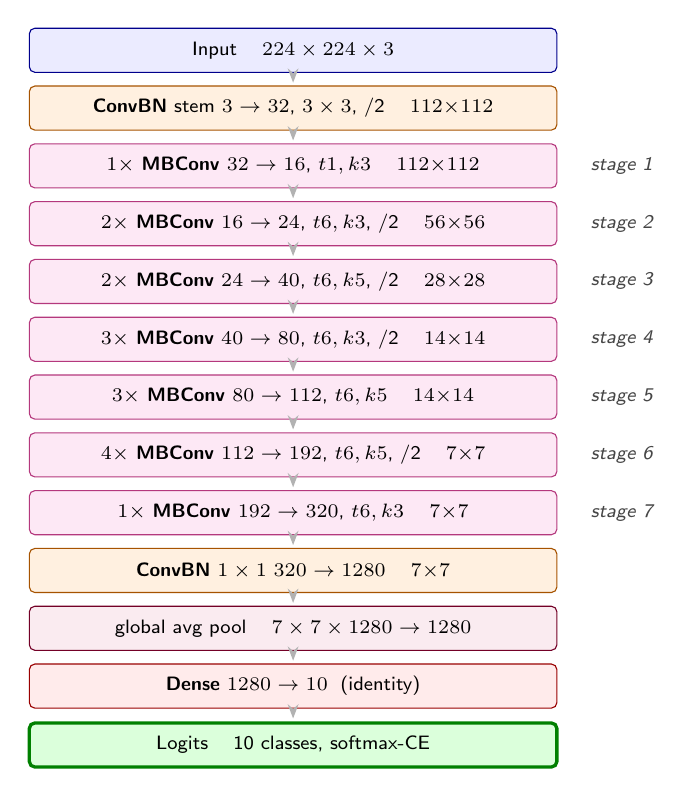
\begin{tikzpicture}[
  >={Stealth[length=1.8mm]},
  every node/.style={font=\sffamily\scriptsize},
  col/.style    = {align=center, rounded corners=2pt, inner sep=2pt, minimum height=0.56cm, minimum width=6.7cm},
  io/.style     = {col, draw=blue!55!black,    fill=blue!8},
  convbn/.style = {col, draw=orange!65!black,  fill=orange!12},
  blk/.style    = {col, draw=magenta!70!black, fill=magenta!9},
  gap/.style    = {col, draw=purple!60!black,  fill=purple!8},
  head/.style   = {col, draw=red!60!black,     fill=red!8},
  logits/.style = {col, draw=green!50!black,   fill=green!14, very thick},
  arr/.style    = {->, thick, gray!60, shorten >=1pt, shorten <=1pt},
  stage/.style  = {font=\sffamily\scriptsize\itshape, gray!55!black, anchor=west},
]
  \node[io]                            (input){Input \;\; $224\times224\times3$};
  \node[convbn, below=0.16cm of input] (stem) {\textbf{ConvBN} stem $3\to32$, $3\times3$, /2 \;\; $112{\times}112$};
  \node[blk, below=0.16cm of stem]     (m1)   {$1\times$ \textbf{MBConv} $32\to16$, $t1,k3$ \;\; $112{\times}112$};
  \node[blk, below=0.16cm of m1]       (m2)   {$2\times$ \textbf{MBConv} $16\to24$, $t6,k3$, /2 \;\; $56{\times}56$};
  \node[blk, below=0.16cm of m2]       (m3)   {$2\times$ \textbf{MBConv} $24\to40$, $t6,k5$, /2 \;\; $28{\times}28$};
  \node[blk, below=0.16cm of m3]       (m4)   {$3\times$ \textbf{MBConv} $40\to80$, $t6,k3$, /2 \;\; $14{\times}14$};
  \node[blk, below=0.16cm of m4]       (m5)   {$3\times$ \textbf{MBConv} $80\to112$, $t6,k5$ \;\; $14{\times}14$};
  \node[blk, below=0.16cm of m5]       (m6)   {$4\times$ \textbf{MBConv} $112\to192$, $t6,k5$, /2 \;\; $7{\times}7$};
  \node[blk, below=0.16cm of m6]       (m7)   {$1\times$ \textbf{MBConv} $192\to320$, $t6,k3$ \;\; $7{\times}7$};
  \node[convbn, below=0.16cm of m7]    (pw)   {\textbf{ConvBN} $1\times1$ $320\to1280$ \;\; $7{\times}7$};
  \node[gap, below=0.16cm of pw]       (g)    {global avg pool \;\; $7\times7\times1280 \to 1280$};
  \node[head, below=0.16cm of g]       (d)    {\textbf{Dense} $1280\to10$ \;(identity)};
  \node[logits, below=0.16cm of d]     (out)  {Logits \;\; 10 classes, softmax-CE};
  \foreach \a/\b in {input/stem,stem/m1,m1/m2,m2/m3,m3/m4,m4/m5,m5/m6,m6/m7,m7/pw,pw/g,g/d,d/out}\draw[arr](\a)--(\b);
  \foreach \n/\k in {m1/1,m2/2,m3/3,m4/4,m5/5,m6/6,m7/7}\node[stage] at ($(\n.east)+(0.30,0)$){stage \k};
\end{tikzpicture}

\vspace{0.45cm}

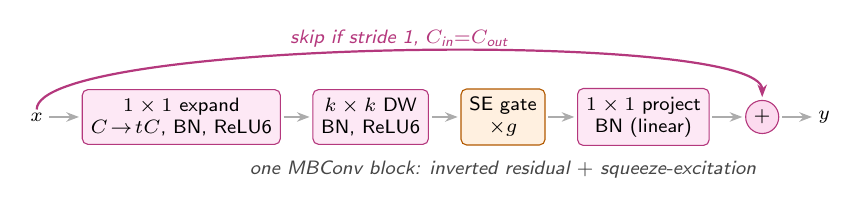
\begin{tikzpicture}[
  >={Stealth[length=1.6mm]},
  every node/.style={font=\sffamily\scriptsize},
  box/.style ={align=center, rounded corners=2pt, inner sep=3pt, minimum height=0.6cm, draw=magenta!70!black, fill=magenta!9},
  se/.style  ={align=center, rounded corners=2pt, inner sep=3pt, minimum height=0.6cm, draw=orange!70!black, fill=orange!12},
  dot/.style ={circle, draw=magenta!70!black, fill=magenta!14, inner sep=0pt, minimum size=0.42cm},
  term/.style={font=\sffamily\scriptsize\itshape, inner sep=1pt},
  arr/.style ={->, thick, gray!65, shorten >=1pt, shorten <=1pt},
  skip/.style={->, thick, magenta!70!black, shorten >=1pt},
]
  \node[term] (x){$x$};
  \node[box, right=0.45cm of x]   (e){$1\times1$ expand\\$C\!\to\!tC$, BN, ReLU6};
  \node[box, right=0.4cm of e]    (dw){$k\times k$ DW\\BN, ReLU6};
  \node[se, right=0.4cm of dw]    (s){SE gate\\$\times g$};
  \node[box, right=0.4cm of s]    (p){$1\times1$ project\\BN (linear)};
  \node[dot, right=0.45cm of p]   (sum){$+$};
  \node[term, right=0.45cm of sum] (y){$y$};
  \foreach \a/\b in {x/e,e/dw,dw/s,s/p,p/sum,sum/y}\draw[arr](\a)--(\b);
  \draw[skip] (x.north) .. controls +(0,0.9) and +(0,0.9) .. (sum.north)
        node[midway, above, term, magenta!70!black]{skip if stride 1, $C_{\text{in}}{=}C_{\text{out}}$};
  \node[term, below=0.16cm of s, gray!55!black]{one MBConv block: inverted residual $+$ squeeze-excitation};
\end{tikzpicture}
\end{center}

\subsection*{The verified trainer}

\S\ref{sec:verified_trainer_pattern} is the pattern and
Chapter~\ref{chap:depthwise} was the first chapter to reuse it. Everything
that carries weight there carries the same weight here, and only the
\texttt{layers} list and the \texttt{bnChannels} that follows from it
are new:

\begin{verbatim}
import LeanMlir

-- 1. The network. `slug` names the committed render, `bnChannels`
--    drives BN threading, `NB` means the BN-followed convs carry
--    no bias.
def efficientnetVerified : VerifiedNetSpec where
  name     := "EfficientNet-B0"
  slug     := "efficientnet"
  inC      := 3
  imageH   := 224
  imageW   := 224
  nClasses := 10
  data     := .imagenette
  layers   := [
    .convBnNB 3 32 3 2,             -- stem 3x3-s2   224->112
    .mbConvSENB  32   32  16  8 3,  -- stage 1, t=1 (no expand)
    .mbConvSENB  16   96  24  4 3,  -- stage 2       112->56
    .mbConvSENB  24  144  24  6 3,
    .mbConvSENB  24  144  40  6 5,  -- stage 3        56->28
    .mbConvSENB  40  240  40 10 5,
    .mbConvSENB  40  240  80 10 3,  -- stage 4        28->14
    .mbConvSENB  80  480  80 20 3,
    .mbConvSENB  80  480  80 20 3,
    .mbConvSENB  80  480 112 20 5,  -- stage 5           @14
    .mbConvSENB 112  672 112 28 5,
    .mbConvSENB 112  672 112 28 5,
    .mbConvSENB 112  672 192 28 5,  -- stage 6        14->7
    .mbConvSENB 192 1152 192 48 5,
    .mbConvSENB 192 1152 192 48 5,
    .mbConvSENB 192 1152 192 48 5,
    .mbConvSENB 192 1152 320 48 3,  -- stage 7            @7
    .convBnNB 320 1280 1 1,         -- head, 1x1 to 1280
    .globalAvgPool,
    .dense 1280 10 ]
  bnChannels := #[32, 32,16, 96,96,24, ... ]  -- all 49, in order

-- 2. The schedule. ResNet-34's and MobileNetV2's, unchanged.
def efficientnetAdamConfig : VerifiedConfig where
  epochs    := 80
  batchSize := 32

-- 3. The entry point: AdamW, cosine with a 3-epoch warmup,
--    baseLR 1e-3.
def main (argv : List String) : IO Unit :=
  efficientnetVerified.toNet.trainAdamSched
    efficientnetAdamConfig (argv.head?.getD "data")
    0.001 0.9 0.999 3 "adam"
\end{verbatim}

\noindent \texttt{.mbConvSENB ic mid oc r k} is one block, not a stage:
there is no repeat count, so the sixteen blocks are sixteen lines and the
stage boundaries are visible as the places where the input width changes.
It takes the \emph{expanded} width \texttt{mid} rather than a ratio \(t\),
which is why the widths read straight off the paper's table, and
\texttt{k} is the depthwise kernel, mixing $3 \times 3$ and $5 \times 5$
by stage. The expand $1 \times 1$ is skipped exactly when
\texttt{mid == ic}, which is stage 1 and its $t=1$.

\textbf{\texttt{r} is the squeeze width, and it is sized off
\texttt{ic}.} Every block in the listing has \texttt{r == ic/4}: 32 gives
8, 16 gives 4, 192 gives 48. That is the correctness note this chapter
returns to in \S\ref{sec:enet_imagenet} from the other direction, and it
is worth reading here first, because sizing the squeeze off the
$6\times$-larger \texttt{mid} instead is the difference between B0's
canonical 5.29M parameters and an inflated 8.4M. The spec is where that
choice is made once and visibly.

\textbf{The arm, and where the SE gate lives in it.}

\begin{verbatim}
  | mbConvSENB ic mid oc r k =>                -- Ch. 7
    (if mid != ic then #[(#[mid,ic,1,1],0),(#[mid],1),(#[mid],2)] else #[])
    ++ #[(#[mid,1,k,k],0),(#[mid],1),(#[mid],2),     -- depthwise kxk + BN
         (#[mid,r],0),(#[r],2),(#[r,mid],0),(#[mid],2),   -- SE: squeeze, excite
         (#[oc,mid,1,1],0),(#[oc],1),(#[oc],2)]     -- project 1x1 + BN
\end{verbatim}

\noindent Same \texttt{mid != ic} conditional as
Chapter~\ref{chap:depthwise}'s, with four tensors inserted in the middle:
\texttt{[mid,r]} down to the squeeze width and \texttt{[r,mid]} back up,
each with a bias. Those two are the only convs in the block that
\emph{keep} their biases, because they are not BN-followed --- the gate
ends in a sigmoid, not a normalizer. That asymmetry is visible in the
arm and nowhere else in the spec.

\textbf{There is no stride argument, and that is deliberate.} B0's
downsampling pattern is fixed by the architecture rather than chosen per
block, so it lives in the renderer, which emits \texttt{b1} as
no-expand, \texttt{b2}, \texttt{b4}, \texttt{b6} and \texttt{b12} as
strided, and the remaining nine as residual. The spec's job is the
\emph{parameter layout}, and \texttt{efficientnetVerified.toSpecs} is
kernel-\texttt{\#guard}ed against an independently audited hand-list. So
the listing above is not a description of the network that got trained,
it is the object the renderer consumed.

\textbf{Forty-nine BatchNorms, and the list is not three per block.}
Every MBConv normalizes after its expand, depthwise and project convs,
which would be $16 \times 3 + 2$ for the stem and head, or 50. Stage 1
has $t=1$ and therefore no expand conv, so it contributes two entries
rather than three, and the real count is 49. \texttt{bnChannels} exists
to get that right: the running-stat region is positional, and an
off-by-one misaligns every frozen statistic downstream of it at
evaluation time.

\textbf{The squeeze-excite biases stay.} \texttt{NB} drops the bias from
every convolution a BatchNorm follows, because the BatchNorm's own shift
absorbs it. SE's two $1 \times 1$s are followed by a sigmoid gate rather
than a BatchNorm, so nothing absorbs theirs and they are kept. The rule
is about what comes \emph{after} a convolution, not about the
convolution.

Every SE block multiplies the input by the sigmoid output of its
two-layer MLP: that is exactly \S~\ref{thm:seBlock_has_vjp} composed with
\S~\ref{thm:elemwiseProduct_has_vjp} and the already-proved dense VJPs
from Chapter~\ref{chap:mlp}. No new math in this chapter beyond the SE
block itself.

\subsection*{Results}

\S\ref{sec:enet_runit} has the run: 80 epochs at about 30 seconds each,
forty and a half minutes, $\mathbf{89.96\%}$ top-1 and $\mathbf{98.45\%}$
top-5, with the loss settling on the same ${\sim}0.50$ label-smoothing
floor as ResNet-34 and MobileNetV2. The three-chapter comparison --- same
dataset, same recipe, same eighty epochs, and every row now a measurement
on the verified XLA path, on one RTX 4060 Ti:

\begin{center}
\begin{tabular}{l r r r r r r}
\hline
Model            & Params  & MLIR       & Step time & Total    & Top-1 & Top-5 \\
\hline
ResNet-34        & 21.29M  & 729\,KB    & 220 ms    & 1.5 h    & 89.71\% & 98.27\% \\
MobileNetV2      &  2.24M  & 1{,}047\,KB &  90 ms   & 35 min   & 89.25\% & \textbf{98.68\%} \\
EfficientNet-B0  &  4.02M  & 1{,}316\,KB & 103 ms   & 41 min   & \textbf{89.96\%} & 98.45\% \\
\hline
\end{tabular}
\end{center}

\noindent Step time is the epoch wall-clock divided by 295 batches, so it
includes each epoch's validation pass. MLIR sizes are the committed
\texttt{<slug>\_adam\_train\_step.mlir} in 1000-byte units.

\begin{itemize}
\item \textbf{EfficientNet-B0 has the best top-1 in the column}, at
  $89.96\%$ against ResNet-34's $89.71\%$ and MobileNetV2's $89.25\%$. It
  gets there with $5.3\times$ fewer parameters than ResNet-34 and in less
  than half the time. MobileNetV2 keeps top-5 by two tenths, which is the
  one place the larger model does not win.

\item \textbf{SE and Swish buy $+0.71$ top-1 over MobileNetV2 for
  $1.80\times$ the parameters} (4.02M against 2.24M). That is a real
  return rather than a bargain: the cost is the two-layer MLP inside
  every one of the sixteen MBConv blocks. Whether $1.8\times$ the
  parameters is worth seven tenths of a point is a judgement, but it is a
  much better trade than it looks on the ImageNet leaderboard, where B0
  is usually compared against far larger models.

\item \textbf{1{,}316\,KB of MLIR is the largest render in the book},
  ahead of MobileNetV2's 1{,}047\,KB and ResNet-34's 729\,KB. The extra
  ops are SE's: each block emits a global-average-pool, two denses, a
  sigmoid and an elementwise multiply, and then the product-rule backward
  for all of it. Sixteen blocks of that is a lot of StableHLO.

\item \textbf{103\,ms per step sits between the two}, slower than
  MobileNetV2's 90\,ms because of exactly those extra ops, and far
  quicker than ResNet-34's 220\,ms because the core is still a depthwise
  sandwich rather than full convolutions.

\item \textbf{The lift is not from SE alone.} EfficientNet's paper thesis
  is \emph{compound scaling}, tuning depth, width and resolution together
  with one coefficient to reach the ImageNet state of the art. At the B0
  baseline shown here SE gives a modest bump, and the real wins arrive at
  B3--B7 where the scaling compounds. This example sits at B0 because the
  dataset is 10-class Imagenette rather than 1000-class ImageNet, and the
  return on scaling saturates much earlier.
\end{itemize}

Every post-2018 vision architecture has some variant of SE in it
(MobileNet V3, EfficientNetV2, ConvNeXt, RegNetZ) because the
accuracy-per-parameter cost is low when you compound it with other
scaling tricks. The other architectural contribution EfficientNet shipped
is the \emph{Swish} activation $\mathrm{swish}(x) = x \cdot \sigma(x)$,
which is orthogonal to SE.

\section{MLIR: Squeeze-and-Excitation}

\noindent\textbf{What is already proven.} Squeeze-excitation is an
elementwise product $\mathrm{se}(x) = x \odot g(x)$, where the per-channel
gate $g(x)$ is itself a small sub-network of the same input $x$:
global-average-pool, dense, swish, dense, sigmoid, broadcast. Because the
gate depends on $x$, the VJP is a \emph{product rule}, not a plain scaling:
\texttt{seBlock\_has\_vjp} proves
\[
  dx = g(x)\odot dy \;+\; g.\mathrm{back}\bigl(x \odot dy\bigr),
\]
the gate-weighted cotangent \emph{plus} the gate's own backward applied to
the co-input $x\odot dy$. \texttt{seBlockFull\_has\_vjp} supplies the
concrete gate (the GAP--dense--swish--dense--sigmoid chain) and
\texttt{mbconvBody\_has\_vjp} composes the whole MBConv.

\medskip\noindent\textbf{The gap and how we close it.} The emitted graph
realizes \texttt{seBlock\_has\_vjp}'s product-rule backward in full. Both
terms are there, and each piece of the gate carries the swish, sigmoid, and
dense bridges of the previous chapters. Here is the fan-in, with the excite
sub-network's internal VJP elided to its one comment line (the SE block runs
on the MBConv's four mid-channels):

\begin{verbatim}
// se = x * broadcast(gate(x)); gate = squeeze-excite sub-network
// %dse = cotangent into the SE block;  %ggb2 = broadcast(gate)
%gdleft = stablehlo.multiply %ggb2, %dse : tensor<1x4x4x4xf32>
%gxdse = stablehlo.multiply %d_s4, %dse : tensor<1x4x4x4xf32>
%gdgate = stablehlo.reduce(%gxdse init: %sc)
            applies stablehlo.add across dimensions = [2, 3]
            : (tensor<1x4x4x4xf32>, tensor<f32>) -> tensor<1x4xf32>
// ... gate VJP through the excite MLP (sigmoid/dense/swish/dense) ...
%gdgate_sp = stablehlo.broadcast_in_dim %gdsq_d, dims = [0, 1]
            : (tensor<1x4xf32>) -> tensor<1x4x4x4xf32>
%gdds = stablehlo.add %gdleft, %gdgate_sp : tensor<1x4x4x4xf32>
\end{verbatim}

\noindent Read it against the product rule:

\begin{itemize}
  \item \texttt{\%gdleft} is $g(x)\odot dy$, the term a naive generator
    would stop at.
  \item \texttt{\%gdgate} reduces $x \odot dy$ over the spatial axes. That
    reduction is the adjoint of the gate's broadcast, so it is the
    cotangent on the per-channel gate values, and it flows back through the
    excite MLP and the global-average-pool to \texttt{\%gdgate\_sp}.
  \item \texttt{\%gdds = \%gdleft + \%gdgate\_sp} adds the two.
\end{itemize}

\noindent That final \texttt{add} \emph{is} the product rule: the gradient
that passes straight through the channel, plus the gradient that re-tunes
the gate, summed.

\medskip\noindent As with attention, the listing shows the new structural
move (the product-rule fan-in) and elides the work behind it: the
\texttt{// gate VJP} comment stands for the excite MLP's own backward
(sigmoid, dense, swish, dense), each carried by this chapter's bridges and
composed in \texttt{seBlockFull\_has\_vjp}.

\medskip\noindent\textbf{Caveats.}
\begin{itemize}
  \item \textbf{The SE fan-in carries no kink condition.} Swish and
    sigmoid are smooth everywhere, and the only smooth-point caveats in an
    MBConv come from its BatchNorms ($\epsilon > 0$).
  \item \textbf{Representative scale} (four mid-channels, two in the squeeze).
\end{itemize}

\section{ImageNet recipe}

\imagenettimmnote
\label{sec:enet_imagenet}

\imagenetphasenote

As with ResNet-34 (Chapter~\ref{chap:residual}) and MobileNet-V2,
the B0 backbone scales to full 1000-class ImageNet unchanged. The
MBConv stack stays put, the head widens to 1000, and the schedule grows.
The spec mirrors \texttt{jax/MainEfficientNetImagenet.lean}:

\begin{verbatim}
-- Same MBConv (SE + Swish) backbone, 1000 classes instead of 10.
def efficientNetB0Imagenet : NetSpec where
  name   := "EfficientNet-B0 (ImageNet, bf16)"
  imageH := 224
  imageW := 224
  layers := [
    .convBn 3 32 3 2 .same,
    .mbConv  32  16 1 3 1 1 true,
    .mbConv  16  24 6 3 2 2 true,
    .mbConv  24  40 6 5 2 2 true,
    .mbConv  40  80 6 3 2 3 true,
    .mbConv  80 112 6 5 1 3 true,
    .mbConv 112 192 6 5 2 4 true,
    .mbConv 192 320 6 3 1 1 true,
    .convBn 320 1280 1 1 .same,
    .globalAvgPool,
    .dense 1280 1000 .identity      -- 1000-class head
  ]

-- The paper's own recipe: RMSProp in TensorFlow's form, exponential
-- LR decay, AutoAugment, stochastic depth, EMA, bf16 conv on.
def efficientNetB0ImagenetConfig : TrainConfig where
  learningRate   := 0.016   -- 0.256@4096, linearly scaled to bs 256
  batchSize      := 256
  epochs         := 80      -- a short check; `Full` below is the 350
                            -- this section reports
  optimizer      := .rmsprop
  momentum       := 0.9     -- mu, for the RMSProp momentum buffer
  rmspropDecay   := 0.9     -- rho, the running mean-square decay
  rmspropEps     := 1e-3
  gradClipNorm   := 0.0     -- OFF: the paper uses none
  weightDecay    := 1e-5    -- small: protects depthwise/SE params
  cosineDecay      := false -- replaced by the paper's exp decay
  expLRDecayRate   := 0.97  -- x0.97 every 2.4 epochs, after warmup
  expLRDecayEpochs := 2.4
  dropout          := 0.2   -- classifier dropout
  warmupEpochs   := 5
  augment        := true
  useAutoAugment := true    -- the full ImageNet policy
  labelSmoothing := 0.1
  bf16           := true
  bf16Conv       := true    -- reaches the MBConv expand/dw/project
  useEMA         := true    -- weight averaging, decay 0.9999
  dropPath       := 0.2     -- stochastic depth (B0 drop-connect rate)
  runningBN      := true    -- eval on running stats, not batch stats

-- The 350-epoch tier is the same recipe, longer.
def efficientNetB0ImagenetConfigFull : TrainConfig :=
  { efficientNetB0ImagenetConfig with epochs := 350 }
\end{verbatim}

\noindent The number this section reports is the \texttt{full} recipe,
the 350-epoch one. The \texttt{default} at 80 epochs is a shorter
validation pass over the identical configuration, useful for checking
that a change trains at all before committing a week of GPU time to it.

Two details are specific to EfficientNet. First, \texttt{bf16Conv}
casts the MBConv block's heavy convolutions (the $1\times1$
expand, the depthwise, the $1\times1$ project) but deliberately
leaves the squeeze-excitation $1\times1$s in fp32: SE acts on a
globally-pooled $1\times1$ tensor where there is no throughput to
win, and its sigmoid gate is precision-sensitive. The payoff is the
same $\sim2\times$ MBConv-block speedup MobileNet sees, from exactly
the convolutions worth casting.

Second, the SE bottleneck is sized off the block's \emph{input}
channels ($c/4$), not the $6\times$-larger expanded width. An earlier
version of the codegen sized it off the expanded width and inflated B0
from its canonical $5.3$M parameters to $8.4$M. Sizing the squeeze
correctly restores the faithful $\mathbf{5.29}$M-parameter B0, which is
the count \S\ref{sec:se_efficientnet_example}'s spec derives today.

\textbf{Augmentation.} The base is Inception-style random-resized-crop
(sampling 8--100\% of the image area at a 3/4--4/3 aspect ratio, resized
to $224\times224$) plus a random horizontal flip, with label smoothing
$0.1$ in the loss, and validation center-crops. On top of that the run
turns on \textbf{AutoAugment}, the full ImageNet policy including its
geometric operations, which is the learned augmentation B0's recipe calls
for. The heavier pack (Mixup, CutMix, RandAugment, Random Erasing) is
wired into the phase-2 Lean$\to$JAX trainer, emitted into the generated
\texttt{tf.data} pipeline with each knob gated on a config flag, and left
off here because the 2019 recipe reaches for AutoAugment instead.

\begin{center}
\begin{tabular}{l l r r r r}
\hline
GPU & Epochs & Per epoch & Wall-clock & Val top-1 & Val top-5 \\
\hline
4$\times$ 4060 Ti & 350 (RMSProp) & $\sim$8.6 min & $\sim$55.5 hr & $\mathbf{76.80\%}$ & $\mathbf{93.26\%}$ \\
\hline
\end{tabular}
\end{center}

\noindent (CUDA, bf16, batch 256.) That is the paper recipe end to end,
and it reached $\mathbf{76.80\%}$ top-1 / $\mathbf{93.26\%}$ top-5 on the
full 50{,}000-image validation split against EfficientNet-B0's published
$77.1\%\,/\,93.3\%$. Getting there took two bug fixes, and neither was
where we first looked.

\textbf{RMSProp: a cautionary result that was really a bug.}
EfficientNet's native optimizer is RMSProp ($\rho=0.9$, $\mu=0.9$,
$\varepsilon=10^{-3}$), and re-running B0 with it exposed what looked
like a learning-rate sensitivity absent from MobileNet-V2's RMSProp: at
the MobileNet-style peak $\mathrm{lr}=0.045$ the loss diverged by epoch
6, and even at the paper's linear-scaled $\mathrm{lr}=0.016$ ($0.256$ at
batch $4096 \to 0.016$ at batch $256$) top-1 \emph{eroded}, peaking
$\sim$31\% near epoch 4, then decaying to $\sim$19\% and stalling. The
obvious workaround was to lower the peak to $\sim$0.01, and for a while
we did. But the learning rate was not the culprit: our RMSProp was not
\emph{TensorFlow's} RMSProp, the variant EfficientNet actually trained
with. Two differences inflate the effective step by up to
$\sim$30$\times$ when the running mean-square is small, which is exactly
the erosion observed. $\varepsilon$ is added \emph{outside} the square
root ($\sqrt{\mathrm{sq}}+\varepsilon$) rather than inside
($\sqrt{\mathrm{sq}+\varepsilon}$), and the mean-square accumulator is
initialized to $0$ rather than $1$. This also explains the MobileNet-V2
contrast: its $\varepsilon=1.0$ is large enough to swamp the
misplacement, so the same bug left it unscathed. MNv2 trained fine on
the buggy optimizer while B0 did not. Correcting both to the TensorFlow
form (\texttt{timm}'s \texttt{RMSpropTF}) let B0 train stably at the
paper's real $0.016$ with no gradient clipping and no lowered LR.

A second bug surfaced once the optimizer was fixed: with the paper's
weight EMA (decay $0.9999$) on, evaluation blew up and validation loss
reached $10^{8}$, because the EMA shadowed only the weights, and eval then
paired those averaged weights with the \emph{live} BatchNorm running
statistics. Shadowing the BN buffers with the same EMA (\texttt{ema\_bn})
fixed it. ConvNeXt uses the identical EMA and never hit this: LayerNorm
has no running buffers to desynchronize, so the bug is specific to
BatchNorm nets trained with weight averaging.

\textbf{The faithful 350-epoch run.} With both fixed, the full tier
reached $\mathbf{76.80\%}$ top-1 / $\mathbf{93.26\%}$ top-5, against
EfficientNet-B0's paper $77.1\%\,/\,93.3\%$: within $0.3\%$ top-1 and
essentially exact on top-5. That tier is the paper recipe end to end,
with RMSProp at $0.016$, AutoAugment, stochastic depth, EMA and
exponential LR decay. A faithful, from-scratch reproduction with no
hacks: real RMSProp, real LR, real EMA. It ran $\sim$55.5\,hr on four
4060 Ti (350 epochs plus eleven 30-minute thermal rests, zero AER). In
the validation curve below, the deliberate slow start is the weight EMA
at $0.9999$ lagging near-init weights until $\sim$epoch 8 before catching
up sharply:

\begin{center}
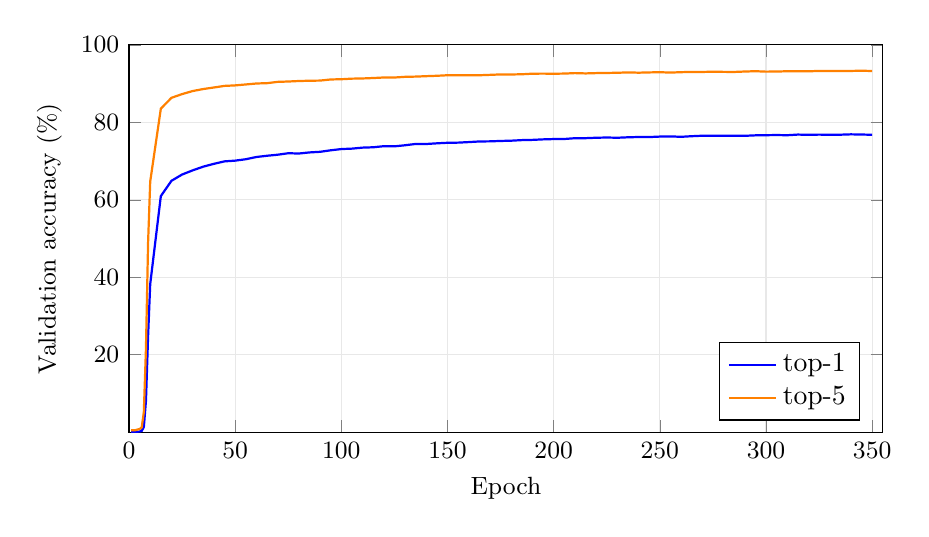
\begin{tikzpicture}
\begin{axis}[
    width=0.92\linewidth, height=6.5cm,
    xlabel={Epoch}, ylabel={Validation accuracy (\%)},
    xmin=0, xmax=355, ymin=0, ymax=100,
    xtick={0,50,100,150,200,250,300,350}, ytick={20,40,60,80,100},
    legend pos=south east, legend cell align={left},
    grid=major, grid style={gray!18},
    tick label style={font=\small}, label style={font=\small},
    every axis plot/.append style={line width=0.8pt, mark=none},
]
\addplot[blue] coordinates {
(1,0.10) (2,0.10) (3,0.10) (4,0.13) (5,0.16) (6,0.33) (7,1.33) (8,8.15) (9,24.81) (10,38.25) (15,60.96) (20,64.91) (25,66.53) (30,67.61) (35,68.57) (40,69.30) (45,69.93) (50,70.12) (55,70.48) (60,71.06) (65,71.38) (70,71.65) (75,72.03) (80,71.96) (85,72.24) (90,72.40) (95,72.79) (100,73.11) (105,73.22) (110,73.48) (115,73.57) (120,73.85) (125,73.81) (130,74.09) (135,74.43) (140,74.42) (145,74.59) (150,74.73) (155,74.77) (160,74.91) (165,75.07) (170,75.10) (175,75.20) (180,75.27) (185,75.42) (190,75.48) (195,75.61) (200,75.69) (205,75.71) (210,75.91) (215,75.92) (220,76.03) (225,76.09) (230,76.03) (235,76.15) (240,76.22) (245,76.21) (250,76.33) (255,76.38) (260,76.27) (265,76.43) (270,76.55) (275,76.52) (280,76.53) (285,76.56) (290,76.53) (295,76.65) (300,76.69) (305,76.73) (310,76.68) (315,76.85) (320,76.78) (325,76.84) (330,76.79) (335,76.82) (340,76.91) (345,76.86) (350,76.80)
};
\addlegendentry{top-1}
\addplot[orange] coordinates {
(1,0.50) (2,0.49) (3,0.52) (4,0.69) (5,0.82) (6,1.24) (7,5.19) (8,21.69) (9,48.97) (10,64.73) (15,83.54) (20,86.34) (25,87.30) (30,88.09) (35,88.61) (40,89.01) (45,89.42) (50,89.55) (55,89.79) (60,90.04) (65,90.12) (70,90.46) (75,90.55) (80,90.68) (85,90.75) (90,90.79) (95,91.08) (100,91.14) (105,91.29) (110,91.34) (115,91.45) (120,91.59) (125,91.58) (130,91.76) (135,91.82) (140,91.93) (145,92.03) (150,92.17) (155,92.15) (160,92.16) (165,92.17) (170,92.27) (175,92.38) (180,92.37) (185,92.42) (190,92.57) (195,92.59) (200,92.56) (205,92.60) (210,92.72) (215,92.64) (220,92.72) (225,92.76) (230,92.81) (235,92.90) (240,92.83) (245,92.90) (250,92.95) (255,92.86) (260,92.96) (265,93.03) (270,93.02) (275,93.08) (280,93.04) (285,93.02) (290,93.13) (295,93.21) (300,93.10) (305,93.13) (310,93.20) (315,93.19) (320,93.19) (325,93.28) (330,93.27) (335,93.27) (340,93.28) (345,93.34) (350,93.26)
};
\addlegendentry{top-5}
\end{axis}
\end{tikzpicture}
\end{center}

\noindent EfficientNet-B0 / ImageNet-1k validation accuracy per epoch,
faithful 350-epoch RMSProp run (bf16, 4$\times$ 4060 Ti). The EMA slow
start (near-zero through $\sim$epoch 7) is the weight average lagging the
live weights, not a training failure, and the final
$76.80\%\,/\,93.26\%$ matches the paper's $77.1\%\,/\,93.3\%$.

\subsection*{Phase 4: the verified trainer}
\label{sec:enet_phase4}

Everything above this point is the phase-2 Lean$\to$JAX trainer. The
phase-4 peer, which trains the same network through the proof-rendered
StableHLO that \S\ref{sec:enet_runit} ran at Imagenette scale, exists and
builds. It is \texttt{apps/imagenette/MainEfficientNetImagenet.lean},
built as \texttt{lake build efficientnet-imagenet-verified}:

\begin{verbatim}
-- Same MBConv + SE backbone, 1000 classes instead of 10.
def efficientnetImagenetVerified : VerifiedNetSpec where
  name       := "EfficientNet-B0 (ImageNet-1k)"
  slug       := "efficientnetin"
  nClasses   := 1000
  data       := .imagenet
  shimScript := "generated_efficientnet_b0_imagenet_shim.py"
  layers     := [ ... the Imagenette stack, 1000-class head ... ]

-- 350 epochs at 64 PER DEVICE; four replicas give the global 256.
-- 350 because that is the schedule the phase-2 number above was
-- measured on.
def efficientnetImagenetConfig : VerifiedConfig where
  epochs    := 350
  batchSize := 64

def main (argv : List String) : IO Unit :=
  efficientnetImagenetVerified.toNet.trainAdamSched
    efficientnetImagenetConfig (argv.head?.getD "data") ... variant
\end{verbatim}

\noindent \texttt{slug} names
\texttt{verified\_mlir/efficientnetin\_<variant>\_train\_step.mlir}, the
rendered graph, and \texttt{shimScript} names this net's own augmentation
shim, which matters more here than it does for MobileNetV2 because
EfficientNet's phase-2 config turns on the full AutoAugment policy and
streaming another net's shim would drop it. The head is the only
parameter shape that moves, from $1280 \times 10$ to $1280 \times 1000$,
which takes the count from 4,020,358 to \textbf{5,288,548}. That second
number is B0's canonical $5.29$M, the count the correctly-sized squeeze
restores.

\medskip\noindent\textbf{This is the first chapter whose phase-4 row could
be measured rather than estimated.} The full paper recipe is already
rendered, and it is rendered data-parallel:
\texttt{efficientnetin\_emarmsdp64dropdo\_train\_step.mlir} carries EMA,
RMSProp, the four-way gradient all-reduce, stochastic depth and
classifier dropout in one graph. Unlike the MobileNetV4 case
Chapter~\ref{chap:depthwise} closes on, this net's collectives are gated
rather than trusted, and by two gates rather than one.
\texttt{tests/TestEfficientNetDpCheck.lean} pins the data-parallel
forward bit-exactly against its single-device peer. That gate hands both
replicas the same rows, so it is structurally blind to a shard-offset
bug, and the \texttt{shard-check} row for \texttt{efficientnet} closes
exactly that hole: it gives the replicas genuinely different data and
checks $\mathrm{DP}([x_A|x_B])$ against the mean of two single-device
steps.

\medskip\noindent\textbf{The variant name is two independent axes, and
that has bitten once.} The optimizer axis and the EMA axis are spelled
separately, so RMSProp-with-EMA is \texttt{emarms}, which does not
\emph{begin} with \texttt{rms}. A driver that tested the variant with a
prefix rather than a substring classified all six \texttt{emarms}
artifacts as non-RMSProp and handed them AdamW's $10^{-3}$ and a cosine
schedule, while the shared trainer's own test, which is a substring,
correctly initialized the RMSProp mean-square to $1.0$. The result was a
run with RMSProp's state, AdamW's learning rate and the wrong schedule,
which descends and prints an entirely normal-looking log.
\texttt{tests/TestVariantPredicates.lean} is the table of these
collisions and this was its first entry.

\medskip\noindent\textbf{The schedule is 350 epochs because the run it
has to match is.} The phase-2 result this net is measured against is the
paper-faithful 350-epoch tier at $76.80\%$, and \texttt{totalSteps} is
what the schedule anneals over, so 80 against 350 is a different
learning-rate curve end to end rather than a shorter version of the same
one. There is a second reason here that MobileNetV2 did not have: no
momentum render exists for \texttt{efficientnetin} at all. The committed
variants are the AdamW family and the RMSProp family, so the 350-epoch
RMSProp tier above is the only phase-2 number these artifacts can be
pointed at.

\medskip\noindent\textbf{What it has not done is run.} No phase-4
ImageNet result exists for this network, which is why every accuracy
above comes from phase 2. What is measured is the throughput, and the
schedule follows from it:

\begin{center}
\begin{tabular}{l r r r r}
\hline
Box & ms/step & min/epoch & 350 epochs & Val top-1 \\
\hline
4$\times$ 4060 Ti (CUDA)  & 181 & 15.1 & $\sim$91.7 h (3.8 d) & TBD \\
4$\times$ 3060 (CUDA)     & 151 & 12.6 & $\sim$77.1 h (3.2 d) & TBD \\
\hline
\end{tabular}
\end{center}

\noindent Set that against the $\sim$8.6 minutes per epoch the phase-2
350-epoch row reports on the same four cards. \textbf{The precision
difference that used to explain this gap is gone}: the verified renders
now carry a bf16 arm, and the row above is measured on it, so both
columns are bf16 over the same architecture. Roughly $1.8\times$ per
epoch survives that change. What is left is the lowerer, not the cast
and not the network.

\noindent\textbf{[TODO: run \texttt{efficientnet-imagenet-verified}.]}

\subsection*{What the EfficientNet recipe changes from the 2018 recipe}

The ResNet-34 trainer of Chapter~\ref{chap:residual} is the
\emph{2018-era} recipe: SGD with momentum plus the ``bag of tricks''
polish (cosine schedule, warmup, label smoothing,
random-resized-crop). The 350-epoch run above is the \emph{2019}
EfficientNet recipe (Tan \& Le), reproduced end to end.
Chapter~\ref{chap:residual}'s RSB-A3 side quest shows what 2021 does
to the 2018 baseline, and Chapter~\ref{chap:layernorm} closes with
2022's version. This table is the 2019 rung of the same ladder. The
\texttt{trainAdamSched} entry point is identical in both columns, and
every row is a one-line change to the \texttt{VerifiedNetSpec}, the
\texttt{VerifiedConfig}, or the arguments beside them:

\begin{center}
\begin{tabular}{@{}l p{2.9cm} p{3.2cm} p{6.3cm}@{}}
\hline
Knob & ResNet-34 (2018) & EfficientNet-B0 (2019) & What the B0 choice buys \\
\hline
Backbone      & basic block, 21.8\,M   & MBConv + SE + Swish, 5.3\,M  & depthwise sandwich + SE gating --- ResNet-34-class accuracy at a quarter of the parameters \\
Optimizer     & SGD + momentum $0.9$   & RMSProp (TF form)             & $\rho{=}0.9$, $\mu{=}0.9$, $\varepsilon{=}10^{-3}$ --- and the exact variant is load-bearing (below) \\
Peak LR       & $0.1$                  & $0.016$                       & linearly scaled from the official $0.256$@4096 --- RMSProp's scale, not comparable to SGD's $0.1$ \\
LR schedule   & cosine to zero         & exponential, $\times0.97$ every 2.4 epochs & the paper's staircase anneal, after the same 5-epoch warmup \\
Epochs        & 90                     & 350                           & the long-schedule regime the regularizers need, and the row the exponential decay above makes non-negotiable \\
Weight decay  & $10^{-4}$, all params  & $10^{-5}$                     & $10\times$ \emph{weaker} --- depthwise and SE parameters are decay-sensitive \\
Augmentation  & RRC + hflip            & + AutoAugment                 & the learned ImageNet policy --- 2019's forerunner of ConvNeXt's DeiT pack \\
Stochastic depth & none                & drop-path $0.2$               & randomly drops whole residual branches per step, at B0's drop-connect rate \\
EMA           & none                   & decay $0.9999$                & evaluates a smoothed shadow of the weights \emph{and} the BN buffers (below) \\
\hline
\end{tabular}
\end{center}

\noindent What carries over unchanged: softmax cross-entropy with
label smoothing $0.1$, the 5-epoch warmup, random-resized-crop +
horizontal flip as the base augmentation, batch 256, train and eval
both at $224$, bf16 matmul and convolution (the SE $1\times1$s in
fp32), and no gradient clipping, which is unlike every later recipe in
this ladder.

The two quietest rows carry the chapter's two debugging lessons.
``RMSProp (TF form)'' is doing real work: as recounted above,
TensorFlow's $\varepsilon$-outside-the-square-root and mean-square
init of $1$ are the difference between training stably at the
paper's $0.016$ and eroding to $\sim$19\%. And the EMA row only
evaluates correctly because the BN running statistics are shadowed
alongside the weights (\texttt{ema\_bn}). Averaged weights
against live BN statistics is an eval blow-up, a failure mode
specific to BatchNorm nets trained with weight averaging.

The through-line of the 2018$\to$2019 shift is \emph{smaller,
longer, more automated}: a quarter of the parameters trained for
$4\times$ the epochs, with a learned augmentation policy, stochastic
depth, and averaged weights supplying the regularization. It is also a
reminder that ``the paper recipe'' includes the optimizer's exact
semantics, not just its hyperparameters.

\section{Side quests}
\label{sec:enet_side_quests}

Three EfficientNet follow-ups extended the family in orthogonal
directions:

\textbf{Noisy Student}
(\href{https://arxiv.org/abs/1911.04252}{Xie et al.\ 2019}).
Semi-supervised distillation that pushed EfficientNet-L2 to
$88.4\%$ top-1 on ImageNet, a state-of-the-art mark at the time. The
recipe: train a teacher on labeled ImageNet, use the teacher to
pseudo-label JFT-300M ($\sim$300M unlabeled images), then train a
larger student on the combined dataset with heavy augmentation
(RandAugment, dropout, stochastic depth), which is the ``noise'' the
title refers to. Iterate.

\textbf{EfficientDet}
(\href{https://arxiv.org/abs/1911.09070}{Tan et al.\ 2020}).
EfficientNet backbone plus \emph{BiFPN} (bidirectional feature
pyramid) for object detection. BiFPN aggregates multi-scale
features by fusing each spatial resolution with both its coarser
and finer neighbors via weighted-sum cross-scale connections. The
detection head is a small per-anchor MLP predicting class plus box
coordinates, applied at every BiFPN output level.

\textbf{EfficientNetV2}
(\href{https://arxiv.org/abs/2104.00298}{Tan \& Le 2021}).
\emph{Fused MBConv} replaces the early stages' expand-$1\times1$ plus
depthwise $k\times k$ with a single regular $k\times k$ convolution ---
more FLOPs, less wall clock, because depthwise convolution is cheap in
arithmetic and expensive in memory traffic, and at low resolution the
traffic dominates. The fused block is already in
the kit as \texttt{.fusedMbConvNB} (\S\ref{sec:mnv4_side_quest}) --- it is
MobileNetV4's stage 0 --- so V2 needs no new primitive, only a spec.

\chapter{ConvNeXt}
\label{chap:layernorm}

\prosesection{ConvNets strike back}

By 2022 the conventional read on image recognition had flipped.
ResNet had been the default backbone for six years. Then in late
2020 ViT (Dosovitskiy et al.,
\href{https://arxiv.org/abs/2010.11929}{arXiv:2010.11929}) showed
that a pure transformer could match or beat ResNet on ImageNet at
sufficient scale, and a year later Swin (Liu et al.\ 2021,
\href{https://arxiv.org/abs/2103.14030}{arXiv:2103.14030}) layered
in hierarchical attention to win COCO/ADE20K on top of that. The
research community's working assumption became ``transformers
beat convnets for vision now.''

ConvNeXt (Liu et al.\ 2022,
\href{https://arxiv.org/abs/2201.03545}{arXiv:2201.03545}) was a
deliberate stress test of that assumption. The authors started
from a standard ResNet-50 and asked: which of the design
differences between ResNet and Swin is actually doing the work?
They proceeded by applying transformer-era choices to the
\emph{ResNet} one at a time and measuring each contribution
in isolation. The full list:

\begin{enumerate}
\item Training recipe modernization (300 epochs, AdamW, RandAug,
  Mixup, CutMix, label smoothing, stochastic depth, layer scale)
\item Stage compute ratio change (from (3, 4, 6, 3) to (3, 3, 9, 3),
  matching Swin)
\item ``Patchify'' stem (replace the 7$\times$7 stride-2 conv with
  a 4$\times$4 stride-4 conv, matching ViT's patch embedding)
\item Depthwise convolutions (split spatial and channel mixing, as
  in MobileNetV2)
\item Inverted bottleneck (1$\times$1 expand 4$\times$, depthwise,
  1$\times$1 project, MobileNetV2-style)
\item Larger kernel (depthwise 7$\times$7 instead of 3$\times$3, to
  approximate Swin's window attention receptive field)
\item Fewer activations and norms (one per block instead of one
  per layer, again matching transformer blocks)
\item LayerNorm instead of BatchNorm
\item GELU instead of ReLU
\end{enumerate}

The result: a model that's pure convolution top to bottom, doesn't
contain a single attention operation, and matches or beats Swin-T
on ImageNet at the same compute budget. The conclusion of the
paper isn't ``convolutions are back.'' It's ``the architectural
gap between ResNet and Swin was mostly the training recipe, not
the receptive field.'' Most of what looked like transformer
superiority was modernization that hadn't been back-ported to the
convnet baseline.

\section{Run it first}
\label{sec:convnext_runit}

Before the two new primitives, train the network that needs them. Four
commands, and the heaviest per-epoch net in the book still finishes
inside an hour and a half:

\begin{verbatim}
lake exe cache get                            # Mathlib oleans, ~30 s
./download_imagenette.sh                      # 330 MB dl, 2.4 GB unpacked
lake build convnext-verified-adam
./.lake/build/bin/convnext-verified-adam data
\end{verbatim}

On one RTX 4060 Ti (CUDA 12.9), from
\texttt{runs/2026-08-12-convnext-imagenette-xla-cuda/}. XLA's startup
banner is removed, the network description line is wrapped, and the
middle of the run is elided:

\begin{verbatim}
[pjrt_ffi] XLA backend: PJRT 0.112, 1 device(s)
[pjrt_ffi] compiled verified_mlir/convnext_adam_train_step.mlir
             (@convnext_adam_train_step, 543 outputs, 1 replica)
             in 6176 ms
[pjrt_ffi] compiled verified_mlir/convnext_fwd.mlir
             (@convnext_fwd, 1 outputs, 1 replica) in 473 ms
ConvNeXt-T on Imagenette 224² (patchify /4 → stem channel-LN →
  [3,3,9,3] blocks @ [96,192,384,768] depthwise-7×7 + channel-LN +
  GELU + layerScale + 3 downsamples 56→7 → GAP → dense)
  via the VERIFIED renderer → XLA/PJRT → GPU
  train 9469, val 3925; bs 32, ConvNeXt-T adam
    (cosine+warmup 3ep, baseLR 0.001000), He init
[pjrt_ffi] RESIDENT: @convnext_adam_train_step holds 540 parameter
             tensors (318.4 MB) on 1 device; they stop crossing PCIe
             from here
Epoch 1/80: loss=2.322982 lr=0.000333
  epoch 1: val_acc = 1485/3925 = 37.834395%  top5 = 2973/3925 = 75.745223%
Epoch 2/80: loss=1.974630 lr=0.000667
  epoch 2: val_acc = 1977/3925 = 50.369427%  top5 = 3485/3925 = 88.789809%
Epoch 3/80: loss=1.691063 lr=0.001000
  epoch 3: val_acc = 2078/3925 = 52.942675%  top5 = 3571/3925 = 90.980892%
Epoch 4/80: loss=1.461296 lr=0.001000
  epoch 4: val_acc = 2295/3925 = 58.471338%  top5 = 3661/3925 = 93.273885%
Epoch 79/80: loss=0.501143 lr=0.000000
  epoch 79: val_acc = 3339/3925 = 85.070064%  top5 = 3819/3925 = 97.299363%
Epoch 80/80: loss=0.501138 lr=0.000000
  epoch 80: val_acc = 3339/3925 = 85.070064%  top5 = 3819/3925 = 97.299363%
done (trained ConvNeXt-T adam + cosine/warmup via packed threading).
\end{verbatim}

Eighty epochs at about 59 seconds each, one hour and nineteen minutes in
total, and \textbf{85.07\%} top-1 with \textbf{97.30\%} top-5 on
Imagenette's 3,925-image validation split. The best epoch reached
$85.22\%$. That is the \emph{lowest} top-1 in this book's Imagenette
column, from much the largest network in it, and
\S\ref{sec:convnext_results} is about why that is the expected answer
rather than a defect.

\medskip\noindent\textbf{Two compile lines, where the previous three
chapters each had three.} ResNet-34, MobileNetV2 and EfficientNet-B0 all
emit a third artifact, \texttt{<slug>\_fwd\_eval}, because BatchNorm
behaves differently in training and in evaluation and the evaluation
forward has to read frozen running statistics. ConvNeXt has no
BatchNorm. LayerNorm computes its statistics from the activation in
front of it every time, so there is nothing to freeze, and the training
forward and the evaluation forward are the same function. The chapter's
central swap pays for itself in the build before it pays for itself in
the mathematics.

\medskip\noindent That also shows in the first four epochs. Top-1 climbs
37.8, 50.4, 52.9, 58.5, smoothly. Chapter~\ref{chap:se} had to explain a
jump at epoch 4, where B0's running statistics were averaging over
weights that were still moving fast and the evaluation forward was
briefly using statistics that no longer described the network. No such
step exists here, because no such statistics exist here.

Three new operations this chapter, still three rules. That run did not
execute a
reimplementation of the network this chapter describes. It executed
\texttt{verified\_mlir/convnext\_adam\_train\_step.mlir}, which is
\texttt{pretty(provenGraph)} off the renderer. Every LayerNorm in it
backpropagates by Theorem~\ref{thm:layerNorm_has_vjp}, every GELU by
Theorem~\ref{thm:gelu_has_vjp}, every layer scale by its own diagonal
adjoint, every depthwise convolution by
Chapter~\ref{chap:depthwise}'s, and every residual skip by
Chapter~\ref{chap:residual}'s additive fan-in.

\medskip\noindent\textbf{And the fold holds at full depth.}
\texttt{convNextForwardTCh\_has\_vjp} chains the patchify stem, all
\emph{eighteen} ConvNeXt blocks, the three downsamples, the pool and the
head through \texttt{vjp\_comp}, with
\texttt{convNextForwardTCh\_has\_vjp\_correct} carrying it back to the
forward the spec denotes. It assumes 22 positive LayerNorm epsilons and
nothing else. Unlike Chapter~\ref{chap:depthwise}, which folds a
representative stem-plus-two-blocks because relu6's kink makes a
whole-network statement false, this one is a single global
\texttt{HasVJP} over the entire network, and it can be because GELU is smooth
everywhere. So for ConvNeXt the accurate sentence is the strong one:
every operation in the graph that just trained carries a proved
backward, and their composition into the whole network carries one too.

\prosesection{Two new primitives}

ConvNeXt requires two activations / normalizations that the
chapters so far haven't needed:

\textbf{LayerNorm} (Ba, Kiros, Hinton 2016,
\href{https://arxiv.org/abs/1607.06450}{arXiv:1607.06450}). BatchNorm
normalizes per-feature across a batch: it relies on the batch having
enough samples for the mean and variance to be stable. That fails for
small batches (memory-constrained training) and for variable-length
sequences (where ``the batch axis'' isn't a clean concept). LayerNorm
solves both by flipping the axis: normalize per-sample across the
feature dimension instead. Same three-term Jacobian cancellation as
BN (Chapter~\ref{chap:bn}), same closed-form backward. Just a
different reduction axis. Theorem~\ref{thm:layerNorm_has_vjp} states
this formally.

\textbf{GELU} (Hendrycks \& Gimpel 2016,
\href{https://arxiv.org/abs/1606.08415}{arXiv:1606.08415}). A smooth
approximation of ReLU: \(\mathrm{GELU}(x) = x \cdot \Phi(x)\), where
\(\Phi\) is the standard-normal CDF. ReLU has a kink at zero, which
forces the codegen to substitute a subgradient convention
(Chapter~\ref{chap:mlp}). GELU is differentiable everywhere, with a
soft-gate behavior near zero that empirically helps transformers
(and, it turns out, modernized CNNs). Diagonal activation Jacobian,
same family as ReLU's diagonal, just with a smooth scalar derivative
instead of an indicator. Theorems
\ref{ax:geluScalar}--\ref{thm:gelu_has_vjp} provide the scalar
function, its derivative, the Jacobian, and the assembled VJP.

Both primitives are used by the upcoming Vision Transformer chapter
(Chapter~\ref{chap:attention}) without modification. ConvNeXt
introduces them here so they're available before ViT needs them.

\prosesection{The ConvNeXt block}

Each ConvNeXt block stacks the modernization items into a single
residual unit:

\[
\text{DW } 7 \times 7 \;\to\; \text{LN} \;\to\;
1 \times 1\ \text{expand } 4\times \;\to\; \text{GELU} \;\to\;
1 \times 1\ \text{project} \;\to\; \text{LayerScale} \;\to\; +\,\text{residual}.
\]

Two pieces: the \emph{inverted bottleneck}
($1 \times 1$ expand 4$\times$, depthwise spatial conv at the wide
point, $1 \times 1$ project) is exactly the MobileNetV2 inverted
residual from Chapter~\ref{chap:depthwise}. ConvNeXt is paying the
MobileNet idea forward. \emph{LayerScale} (Touvron et al.\ 2021) is
a learnable per-channel scalar \(\gamma\) initialized to \(10^{-6}\)
that multiplies the block's contribution before the residual add,
keeping the block near-identity at init in the same spirit as
ResNet's residual. The spec's \texttt{.convNextStage} primitive
emits \(N\) of these blocks at fixed channel width. The
\texttt{.convNextDownsample} primitive emits the LN + $2 \times 2$
stride-2 conv that transitions between stages.

\prosesection{ConvNeXt-T is four stages, ResNet-style}

The full ConvNeXt-T spec is the same stem--stages--head template
as ResNet-34. A $4 \times 4$ stride-4 ``patchify'' stem replaces
the $7 \times 7$ stride-2 stem. Four stages with block counts
\((3, 3, 9, 3)\) at channel widths \((96, 192, 384, 768)\) replace
the ResNet stages. A final global-average-pool plus 768-to-10
dense replaces the head. Total: 27.8M parameters, comparable to
ResNet-50. Every architectural primitive in the spec is now
codegen-backed and has a proved VJP. None of the math in this
chapter is genuinely new beyond the LayerNorm-axis rotation and
the GELU smoothness.

With a modernized convnet backbone, the dominant axis of
variation between runs becomes the \emph{training recipe}, not
the architecture. The example section below makes that
concrete. The chapter
closes by putting the full recipe side-by-side with the 2018
ResNet-34 recipe of
Chapter~\ref{chap:residual}, knob by knob: the four-year jump in
how convnets are trained, on one page.

\section{The theorems}

\begin{definition}[GELU scalar function]
  \label{ax:geluScalar}
  \lean{Proofs.geluScalar}
  \leanok
  The tanh approximation the codegen actually emits (not the exact
  \(x \cdot \Phi(x)\) erf form):
  \(\mathrm{geluScalar}(x) = 0.5\, x\, \bigl(1 + \tanh(\sqrt{2/\pi}\,
  (x + 0.044715\, x^3))\bigr)\).
\end{definition}

\begin{definition}[GELU scalar derivative]
  \label{ax:geluScalarDeriv}
  \lean{Proofs.geluScalarDeriv}
  \leanok
  \uses{ax:geluScalar}
  Defined as Mathlib's \(\mathrm{deriv}\, \mathrm{geluScalar}\) --- so
  the connection to the forward is automatic, not asserted. The
  closed form (what the verified \texttt{geluBack} emitter renders) is
  the separate theorem \texttt{geluScalarDeriv\_eq}, proved by
  assembling \texttt{HasDerivAt} for the inner polynomial, \(\tanh\)
  (via \(\tanh = \sinh/\cosh\) and the quotient rule), and the outer
  product.
\end{definition}

\begin{theorem}[GELU Jacobian]
  \label{ax:pdiv_gelu}
  \lean{Proofs.pdiv_gelu}
  \leanok
  \uses{ax:pdiv, ax:geluScalarDeriv}
  \Prove{} \(\pdiv(\mathrm{gelu})\, x\, i\, j
    = \delta_{ij} \cdot \mathrm{geluScalar}'(x_i)\) --- the diagonal
  activation Jacobian.
\end{theorem}

\begin{proof}
\leanok
\emph{Sketch: the template for every elementwise activation with a
smooth scalar function --- extract one output coordinate, factor it
through a projection, convert back to the scalar derivative.}
\begin{enumerate}
  \item \(\pdiv(\mathrm{gelu})\, x\, i\, j
          = \fderiv_{\R}\,(y \mapsto \mathrm{gelu}(y)_j)\, x\, (\basisVec_i)\).
    \pf{Definition~\ref{ax:pdiv} and \texttt{fderiv\_apply};
    \(\mathrm{gelu}\) is differentiable because
    \(\mathrm{geluScalar}\) is (tanh is differentiable everywhere,
    via \(\tanh = \sinh/\cosh\) with \(\cosh > 0\)).}
  \item \(y \mapsto \mathrm{gelu}(y)_j
          = \mathrm{geluScalar} \circ \mathrm{proj}_j\), so its
    derivative is
    \(\fderiv\,\mathrm{geluScalar}\,(x_j) \circ \mathrm{proj}_j\).
    \pf{Chain rule (Mathlib's \texttt{fderiv\_comp});
    \(\mathrm{proj}_j\) is a continuous linear map, its own
    derivative.}
  \item Evaluate at \(\basisVec_i\):
    \(\mathrm{proj}_j(\basisVec_i) = \delta_{ji}\), and the scalar
    \(\fderiv\) converts to \(\mathrm{deriv}\)
    (\texttt{fderiv\_eq\_smul\_deriv}), giving
    \(\delta_{ji} \cdot \mathrm{deriv}\,\mathrm{geluScalar}\,(x_j)\).
  \item \Qed{}
    \pf{Case split on \(i = j\); when they coincide,
    \(\mathrm{deriv}\,\mathrm{geluScalar}\,(x_i)\) \emph{is}
    \(\mathrm{geluScalar}'(x_i)\) by
    Definition~\ref{ax:geluScalarDeriv}.}
\end{enumerate}
\end{proof}

\begin{theorem}[LayerNorm VJP]
  \label{thm:layerNorm_has_vjp}
  \lean{Proofs.layerNorm_has_vjp}
  \leanok
  \uses{thm:bn_has_vjp}
  \Assume{}
  \begin{enumerate}
    \item \(\varepsilon > 0\) \hfill[\texttt{h\(\varepsilon\)}]
  \end{enumerate}
  \Prove{} \(\HasVJP\, (\mathrm{layerNormForward})\).
\end{theorem}

\begin{proof}
\leanok
\begin{enumerate}
  \item \(\mathrm{layerNormForward} = \mathrm{bnForward}\),
    definitionally: on a single feature vector, LayerNorm \emph{is}
    the 1D normalization primitive --- the BN/LN distinction (which
    axis, running statistics) is an engineering concern that
    dissolves at the per-vector math level.
  \item \Qed{}
    \pf{Theorem~\ref{thm:bn_has_vjp} applies verbatim, with
    assumption 1 as its \(\varepsilon > 0\) hypothesis.}
\end{enumerate}
\end{proof}

\begin{theorem}[GELU VJP]
  \label{thm:gelu_has_vjp}
  \lean{Proofs.gelu_has_vjp}
  \leanok
  \uses{ax:pdiv_gelu, def:hasvjp}
  \(\HasVJP\, (\mathrm{gelu})\), with backward
  \(B(x, dy)_i = dy_i \cdot \mathrm{geluScalar}'(x_i)\).
\end{theorem}

\begin{proof}
\leanok
\begin{enumerate}
  \item \Suffices{} \(B(x, dy)_i = \sum_j \pdiv(\mathrm{gelu})\,
    x\, i\, j \cdot dy_j\). \pf{Definition~\ref{def:hasvjp}.}
  \item \Qed{}
    \pf{By the GELU Jacobian (Theorem~\ref{ax:pdiv_gelu}) the sum is
    diagonal and collapses at \(j = i\) to
    \(\mathrm{geluScalar}'(x_i) \cdot dy_i\). Same template as ReLU,
    Swish, h-swish: diagonal Jacobian \(\Rightarrow\) one-step VJP.}
\end{enumerate}
\end{proof}

\section{Example: ConvNeXt-T on Imagenette}
\label{sec:convnext_example}

ConvNeXt (Liu et al.\ 2022,
\href{https://arxiv.org/abs/2201.03545}{arXiv:2201.03545}) was the
``ConvNets strike back'' paper: a deliberate back-port of design
choices from the Swin Transformer back into a pure CNN, asking
which of those choices were doing the actual work. The answer:
depthwise $7 \times 7$ convs at lower channel counts, LayerNorm
instead of BatchNorm, GELU instead of ReLU, and an inverted-
bottleneck-style $4\times$ expansion in every block. None of those
ingredients are transformer-specific. The architecture below is
pure convolution top to bottom. The modernization is in the
\emph{recipe}, not the receptive field.

ConvNeXt-T is the smallest variant in the paper, $\sim$28M params
(roughly the parameter budget of ResNet-50). At ImageNet-1K scale
the paper reports $82.1\%$ top-1, beating Swin-T at the same
compute budget. At our 9.5K-image Imagenette scale, the data
regime is different but the architectural story still holds.

\subsection*{The architecture}

ConvNeXt-Tiny replaces the convolutional stages with
\texttt{.convNextStage} blocks at four widths ($96, 192, 384, 768$)
and depths ($3, 3, 9, 3$), glued by \texttt{.convNextDownsample} transitions
(LayerNorm $+$ $2 \times 2$ stride-2 conv). A $4 \times 4$ stride-4
patchify stem and a global-average-pool head bracket the stack. The
inset shows one ConvNeXt block: an inverted bottleneck with a single
LayerNorm and GELU, scaled by a learnable $\gamma$ before the residual
add.

\begin{center}
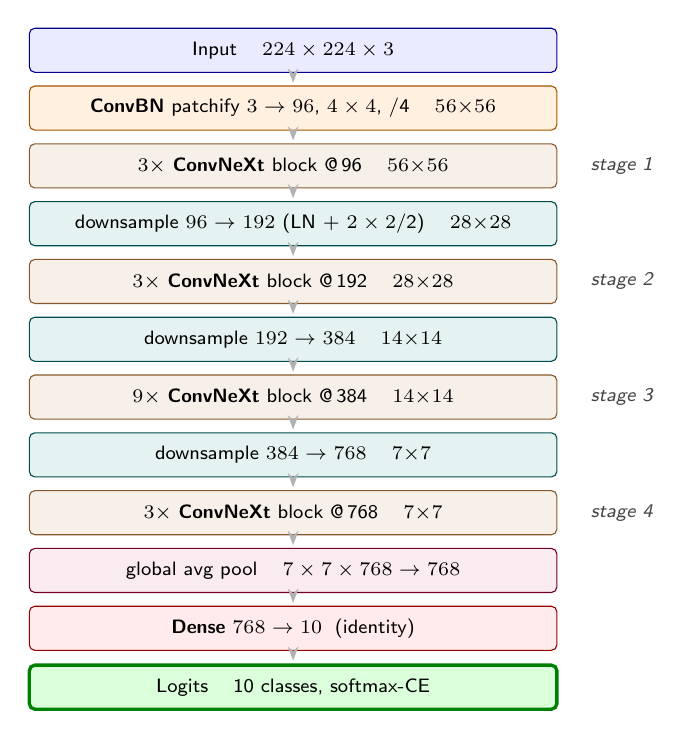
\begin{tikzpicture}[
  >={Stealth[length=1.8mm]},
  every node/.style={font=\sffamily\scriptsize},
  col/.style    = {align=center, rounded corners=2pt, inner sep=2pt, minimum height=0.56cm, minimum width=6.7cm},
  io/.style     = {col, draw=blue!55!black,   fill=blue!8},
  convbn/.style = {col, draw=orange!65!black, fill=orange!12},
  blk/.style    = {col, draw=brown!70!black,  fill=brown!12},
  norm/.style   = {col, draw=teal!60!black,   fill=teal!10},
  gap/.style    = {col, draw=purple!60!black, fill=purple!8},
  head/.style   = {col, draw=red!60!black,    fill=red!8},
  logits/.style = {col, draw=green!50!black,  fill=green!14, very thick},
  arr/.style    = {->, thick, gray!60, shorten >=1pt, shorten <=1pt},
  stage/.style  = {font=\sffamily\scriptsize\itshape, gray!55!black, anchor=west},
]
  \node[io]                          (input){Input \;\; $224\times224\times3$};
  \node[convbn, below=0.16cm of input] (stem) {\textbf{ConvBN} patchify $3\to96$, $4\times4$, /4 \;\; $56{\times}56$};
  \node[blk, below=0.16cm of stem]   (c1)   {$3\times$ \textbf{ConvNeXt} block @\,96 \;\; $56{\times}56$};
  \node[norm, below=0.16cm of c1]    (n1)   {downsample $96\to192$ (LN $+$ $2\times2$/2) \;\; $28{\times}28$};
  \node[blk, below=0.16cm of n1]     (c2)   {$3\times$ \textbf{ConvNeXt} block @\,192 \;\; $28{\times}28$};
  \node[norm, below=0.16cm of c2]    (n2)   {downsample $192\to384$ \;\; $14{\times}14$};
  \node[blk, below=0.16cm of n2]     (c3)   {$9\times$ \textbf{ConvNeXt} block @\,384 \;\; $14{\times}14$};
  \node[norm, below=0.16cm of c3]    (n3)   {downsample $384\to768$ \;\; $7{\times}7$};
  \node[blk, below=0.16cm of n3]     (c4)   {$3\times$ \textbf{ConvNeXt} block @\,768 \;\; $7{\times}7$};
  \node[gap, below=0.16cm of c4]     (g)    {global avg pool \;\; $7\times7\times768 \to 768$};
  \node[head, below=0.16cm of g]     (d)    {\textbf{Dense} $768\to10$ \;(identity)};
  \node[logits, below=0.16cm of d]   (out)  {Logits \;\; 10 classes, softmax-CE};
  \foreach \a/\b in {input/stem,stem/c1,c1/n1,n1/c2,c2/n2,n2/c3,c3/n3,n3/c4,c4/g,g/d,d/out}
     \draw[arr](\a)--(\b);
  \foreach \n/\k in {c1/1,c2/2,c3/3,c4/4}\node[stage] at ($(\n.east)+(0.30,0)$){stage \k};
\end{tikzpicture}

\vspace{0.45cm}

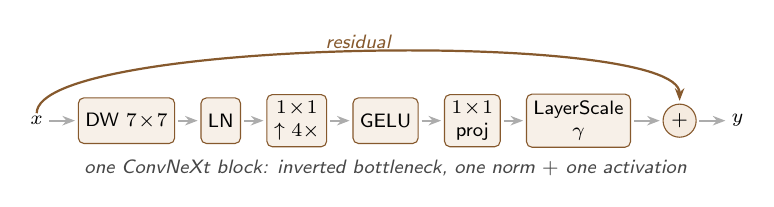
\begin{tikzpicture}[
  >={Stealth[length=1.6mm]},
  every node/.style={font=\sffamily\scriptsize},
  box/.style  = {align=center, rounded corners=2pt, inner sep=2.5pt, minimum height=0.58cm, draw=brown!70!black, fill=brown!12},
  dot/.style  = {circle, draw=brown!70!black, fill=brown!16, inner sep=0pt, minimum size=0.42cm},
  term/.style = {font=\sffamily\scriptsize\itshape, inner sep=1pt},
  arr/.style  = {->, thick, gray!65, shorten >=1pt, shorten <=1pt},
  skip/.style = {->, thick, brown!70!black, shorten >=1pt},
]
  \node[term] (x){$x$};
  \node[box, right=0.4cm of x]  (dw){DW $7\!\times\!7$};
  \node[box, right=0.32cm of dw](ln){LN};
  \node[box, right=0.32cm of ln](ex){$1\!\times\!1$\\$\uparrow4\times$};
  \node[box, right=0.32cm of ex](ge){GELU};
  \node[box, right=0.32cm of ge](pr){$1\!\times\!1$\\proj};
  \node[box, right=0.32cm of pr](ls){LayerScale\\$\gamma$};
  \node[dot, right=0.4cm of ls] (sum){$+$};
  \node[term, right=0.4cm of sum](y){$y$};
  \foreach \a/\b in {x/dw,dw/ln,ln/ex,ex/ge,ge/pr,pr/ls,ls/sum,sum/y}\draw[arr](\a)--(\b);
  \draw[skip] (x.north) .. controls +(0,0.95) and +(0,0.95) .. (sum.north)
        node[midway, above, term, brown!70!black]{residual};
  \node[term, below=0.16cm of ge, gray!55!black]{one ConvNeXt block: inverted bottleneck, one norm $+$ one activation};
\end{tikzpicture}
\end{center}

\subsection*{The verified trainer}

\S\ref{sec:verified_trainer_pattern} is the pattern, and every chapter
since Chapter~\ref{chap:depthwise} has reused it. ConvNeXt drops one of
its four annotated points. There is no \texttt{bnChannels} here, because
there is no BatchNorm.

\begin{verbatim}
import LeanMlir

-- 1. The network. `slug` names the committed render. No `bnChannels`:
--    LayerNorm keeps no running statistics, so nothing has to be
--    threaded from training into evaluation.
def convnextVerified : VerifiedNetSpec where
  name     := "ConvNeXt-T"
  slug     := "convnext"
  inC      := 3
  imageH   := 224
  imageW   := 224
  nClasses := 10
  data     := .imagenette
  layers   := [
    .conv 3 96 4 4, .layerNorm 96,       -- patchify 4x4/s4 + stem LN
    .convNextBlockCh 96,  .convNextBlockCh 96,  .convNextBlockCh 96,
    .layerNorm 96,  .conv 96 192 2 2,    -- downsample  96->192, 56->28
    .convNextBlockCh 192, .convNextBlockCh 192, .convNextBlockCh 192,
    .layerNorm 192, .conv 192 384 2 2,   -- downsample 192->384, 28->14
    .convNextBlockCh 384, .convNextBlockCh 384, .convNextBlockCh 384,
    .convNextBlockCh 384, .convNextBlockCh 384, .convNextBlockCh 384,
    .convNextBlockCh 384, .convNextBlockCh 384, .convNextBlockCh 384,
    .layerNorm 384, .conv 384 768 2 2,   -- downsample 384->768, 14->7
    .convNextBlockCh 768, .convNextBlockCh 768, .convNextBlockCh 768,
    .globalAvgPool, .dense 768 10 ]      -- head
  -- Stochastic depth, read only by the `*drop` variants: one global
  -- block index, keep_i = 1 - 0.1*i/17 at all eighteen blocks.
  dropKeeps := (Array.range 18).map (fun i =>
                 1.0 - 0.1 * i.toFloat / 17.0)

-- 2. The schedule. ResNet-34's, MobileNetV2's and B0's, unchanged.
def convnextAdamConfig : VerifiedConfig where
  epochs    := 80
  batchSize := 32

-- 3. The entry point: AdamW, cosine with a 3-epoch warmup,
--    baseLR 1e-3.
def main (argv : List String) : IO Unit :=
  convnextVerified.toNet.trainAdamSched
    convnextAdamConfig (argv.head?.getD "data")
    0.001 0.9 0.999 3 "adam"
\end{verbatim}

\noindent The structure follows the paper's macro-design prescription:
4 stages with block counts $(3, 3, 9, 3)$ and channels doubling on
every downsample $(96 \to 192 \to 384 \to 768)$, with the heavy
9-block stage at the $14 \times 14$ / 384-channel resolution. The stem
is a $4 \times 4$ stride-4 conv (mirrored from ViT's patch-embed), not
the $7 \times 7$ stride-2 stem of a ResNet, and that is one of the
seven modernization-recipe items called out in the paper. The same base
recipe as the EnetB0 chapter (Adam @ 0.001, cosine, warmup-3,
WD 1e-4, label smoothing 0.1) keeps the cross-architecture
comparison clean.

\textbf{\texttt{.convNextBlockCh c} is one block, not a stage.} There is
no repeat count, so the eighteen blocks are eighteen entries and the
stage boundaries are visible as the places where the width changes.
\texttt{Ch} names the norm: the LayerNorm inside the block reduces over
the \texttt{c} channels at each spatial position, which is ConvNeXt's
real normalization rather than the scalar reduction the bare name
suggests.

\textbf{The arm, and the one tensor with no partner.}

\begin{verbatim}
  | layerNorm d      => #[(#[d],1),(#[d],2)]           -- Ch. 8: gamma, beta
  | convNextBlockCh c =>                               -- Ch. 8
    #[(#[c,1,7,7],0),(#[c],2),(#[c],1),(#[c],2),       -- dw 7x7 + LN(gamma,beta)
      (#[4*c,c,1,1],0),(#[4*c],2),                     -- expand 1x1 (4x)
      (#[c,4*c,1,1],0),(#[c],2),                       -- project 1x1
      (#[c],1)]                                        -- layer scale
\end{verbatim}

\noindent Eight of those nine tensors pair off into weight-and-bias or
$\gamma$-and-$\beta$. The ninth, the trailing \texttt{(\#[c],1)}, has no
partner: layer scale is a single learned per-channel multiplier with
nothing added after it, initialised to ones so a fresh block is the
identity on its residual branch. It is the smallest parameter in the
chapter and the one whose backward is a pure diagonal.

\textbf{The stem and the downsamples are spelled out, not packaged.} A
\texttt{.convNextDownsample 96 192} is two entries here, a
\texttt{.layerNorm 96} and a \texttt{.conv 96 192 2 2}, and the patchify
stem is likewise a \texttt{.conv} followed by a \texttt{.layerNorm}. The
spec's job is the \emph{parameter layout}, not the block vocabulary, so
it names weights rather than concepts.

\textbf{180 parameter tensors, 27,826,282 scalars.}
\texttt{convnextVerified.toSpecs} is kernel-\texttt{\#guard}ed against
\texttt{ConvNeXtLayout.specs}, an independently audited hand-list, and
the ImageNet spec of \S\ref{sec:convnext_imagenet} is pinned to this one
at everything but its head. At 1000 classes the count is 28,587,592,
which is the JAX reference's own figure exactly. So the listing above is
not a description of the network that got trained, it is the object the
renderer consumed.

\textbf{Twenty-two LayerNorms are the entire hypothesis budget.} One in
the stem, one per block, one per downsample, and no head LN.
Theorem~\ref{thm:layerNorm_has_vjp} wants $\varepsilon > 0$ at each, and
those 22 positivities are the only assumptions anywhere in the chain.

\subsection*{Results}
\label{sec:convnext_results}

\S\ref{sec:convnext_runit} has the run: 80 epochs at about 59 seconds
each, one hour and nineteen minutes, $\mathbf{85.07\%}$ top-1 and
$\mathbf{97.30\%}$ top-5, with the loss settling on the same
${\sim}0.50$ label-smoothing floor as the three chapters before it. The
four-chapter comparison --- same dataset, same recipe, same eighty epochs,
and every row a measurement on the verified XLA path, on one RTX 4060 Ti:

\begin{center}
\begin{tabular}{l r r r r r r}
\hline
Model            & Params  & MLIR       & Step time & Total    & Top-1 & Top-5 \\
\hline
ResNet-34        & 21.29M  & 729\,KB    & 220 ms    & 1.5 h    & 89.71\% & 98.27\% \\
MobileNetV2      &  2.24M  & 1{,}047\,KB &  90 ms   & 35 min   & 89.25\% & \textbf{98.68\%} \\
EfficientNet-B0  &  4.02M  & 1{,}316\,KB & 103 ms   & 41 min   & \textbf{89.96\%} & 98.45\% \\
ConvNeXt-T       & \textbf{27.83M} & 985\,KB & 196 ms & 1.3 h  & 85.07\% & 97.30\% \\
\hline
\end{tabular}
\end{center}

\noindent Step time is the epoch wall-clock divided by 295 batches, so it
includes each epoch's validation pass. MLIR sizes are the committed
\texttt{<slug>\_adam\_train\_step.mlir} in 1000-byte units.

\begin{itemize}
  \item \textbf{The largest network in the column finishes last}, and by
    a clear margin: $85.07\%$ against EfficientNet-B0's $89.96\%$, from
    $6.9\times$ the parameters. Two things contribute. ConvNeXt-T carries
    27.83M parameters against 9,469 training images, which is not the
    data scale that capacity wants. And the recipe here is the shared
    one, Adam at $10^{-3}$ with cosine and label smoothing, which is
    deliberately \emph{not} the recipe ConvNeXt was designed around.
  \item \textbf{That is the chapter's thesis arriving as a result rather
    than a claim.} ConvNeXt's paper argues the modernization lives in the
    training recipe, so a ConvNeXt run on somebody else's recipe should
    underperform, and it does. \S\ref{sec:convnext_imagenet} is the
    control: the same architecture, given the full DeiT pack and 300
    epochs, reaches $81.10\%$ on ImageNet-1k and beats every other
    network in this book. The architecture was never the variable.
  \item \textbf{It is no longer the slowest per step.} At 196 ms
    ConvNeXt-T sits under ResNet-34's 220 ms, which reverses the ordering
    the phase-3 numbers showed, where ConvNeXt was slowest by $1.45\times$.
    The depthwise $7 \times 7$ and the channel LayerNorms still touch
    every spatial position twice per block, but that costs less than
    ResNet-34's dense $3 \times 3$ stacks once both graphs go through the
    same compiler.
  \item \textbf{The MLIR is mid-pack at 985\,KB}, above ResNet-34's 729
    and below MobileNetV2's 1,047 and EfficientNet-B0's 1,316. Block
    count is not what separates them, since ConvNeXt's eighteen is more
    than either. What separates them is what one block costs to emit:
    ConvNeXt spends three convolutions and a single LayerNorm per block,
    while an inverted residual spends three convolutions and three
    BatchNorms, and an MBConv adds the squeeze-excitation pair on top of
    that. One normalization per block instead of one per layer was item
    seven on the modernization list, and it is visible in the file size.
\end{itemize}

\section{MLIR: Layer Scale}

Layer scale is a per-channel learnable diagonal,
$\mathrm{layerScale}(\gamma, x) = \gamma \odot x$, and it is the simplest
operator in this series. Its Jacobian is diagonal, so it is its own adjoint:
\texttt{layerScale\_has\_vjp} proves $\mathrm{back}(x, dy) = \gamma \odot dy$,
the backward multiplying by the \emph{same} $\gamma$ the forward did. There is
nothing to bridge past that identity, so the emitted graph is two
\texttt{multiply}s against one tensor:

\begin{verbatim}
// ConvNeXt block tail:  out = x + layerScale(gamma, project(...))
%ls  = stablehlo.multiply %gls, %pr   : tensor<1x2x4x4xf32> // gamma (*) pr
%out = stablehlo.add %x, %ls          : tensor<1x2x4x4xf32> // + identity skip
// backward, cotangent %dOut:  d(pr) = gamma (*) d(out)
%dpr = stablehlo.multiply %gls, %dOut : tensor<1x2x4x4xf32>
\end{verbatim}

\noindent The forward \texttt{multiply \%gls, \%pr} and the backward
\texttt{multiply \%gls, \%dOut} are the same op against the same $\gamma$
tensor: a diagonal map is its own transpose, so its VJP is itself. The
identity skip is the residual fan-in of Chapter~\ref{chap:residual}. The
surrounding GELU, LayerNorm, and convolution backwards reuse their bridges.
Uniquely in this book, every one is unconditional (the only hypothesis
anywhere is LayerNorm's $\epsilon > 0$). The full block is
$\mathrm{residual}(\mathrm{layerScale} \circ \mathrm{project} \circ
\mathrm{gelu} \circ \mathrm{expand} \circ \mathrm{LN} \circ
\mathrm{depthwise})$, composed by \texttt{convNextBlock\_has\_vjp}.

\section{ImageNet recipe}

\imagenettimmnote
\label{sec:convnext_imagenet}

\imagenetphasenote

ConvNeXt's architecture reached this book through the Imagenette
example earlier in this chapter. The phase-2 port wires the two
ConvNeXt-specific layers (\texttt{.convNextStage},
\texttt{.convNextDownsample}) into the JAX codegen. Because that path
differentiates with \texttt{jax.value\_and\_grad}, only the forward
had to be written, and the backward comes for free. The spec mirrors
\texttt{jax/MainConvNeXtImagenet.lean}:

\begin{verbatim}
-- Faithful patchify stem, stage/downsample backbone, 1000 classes.
def convNeXtTinyImagenet : NetSpec where
  name   := "ConvNeXt-T (ImageNet, bf16)"
  imageH := 224
  imageW := 224
  layers := [
    .convNextStem 3 96 4,              -- patchify: 4x4 s4 conv -> channel-LN (no BN/ReLU)
    .convNextStage 96 3 .ln .gelu,     -- stage 1: 3 blocks @ 96  (56x56)
    .convNextDownsample 96 192,        -- 56 -> 28
    .convNextStage 192 3 .ln .gelu,    -- stage 2: 3 blocks @ 192
    .convNextDownsample 192 384,       -- 28 -> 14
    .convNextStage 384 9 .ln .gelu,    -- stage 3: 9 blocks @ 384
    .convNextDownsample 384 768,       -- 14 -> 7
    .convNextStage 768 3 .ln .gelu,    -- stage 4: 3 blocks @ 768
    .globalAvgPool,
    .dense 768 1000 .identity          -- 1000-class head
  ]

-- ConvNeXt needs AdamW, not SGD; full DeiT-style recipe.
def convNeXtTinyImagenetConfig : TrainConfig where
  learningRate      := 2.5e-4       -- 4e-3 @ batch 4096, linearly scaled to 256
  batchSize         := 256
  epochs            := 80           -- validation tier of an 80->300 ladder
  useAdam           := true         -- AdamW (decoupled weight decay)
  weightDecay       := 0.05
  wdExcludeNormBias := true         -- timm no_weight_decay: skip norm g/b, bias, LayerScale
  cosineDecay       := true
  warmupEpochs      := 20           -- ConvNeXt paper warmup (was 5)
  gradClipNorm      := 1.0          -- cheap insurance (unlocked the ViT run)
  augment           := true
  useRandAugment    := true         -- geometric RandAugment N=2, M=9, mstd0.5, inc1
  randAugmentGeometric := true
  useMixup          := true         -- Mixup alpha 0.8 ...
  useCutmix         := true         -- ... + CutMix alpha 1.0 (alternates per step) ...
  randomErasing     := true         -- ... + Random Erasing p 0.25 (full DeiT pack)
  labelSmoothing    := 0.1
  bf16              := true
  bf16Conv          := true         -- dw-7x7 + 1x1s; LN/GELU stay fp32
  useEMA            := true         -- weight averaging, decay 0.9999
  dropPath          := 0.1          -- stochastic depth (ConvNeXt-T paper value)

-- 300-epoch "full" tier: same config, longer schedule.
def convNeXtTinyImagenetConfigFull : TrainConfig :=
  { convNeXtTinyImagenetConfig with epochs := 300 }
\end{verbatim}

Unlike MobileNet and EfficientNet, ConvNeXt trains with AdamW and a
small decoupled weight decay, not SGD. The modernized-convnet
recipe is the architecture's whole thesis. \texttt{bf16Conv} pays off
especially here: the $7\times7$ depthwise is $\sim2.3\times$ faster
in bfloat16 (a large kernel has enough arithmetic for the tensor
cores to bite, unlike the $3\times3$ depthwise, which is a wash), and
the inverted-bottleneck $1\times1$s are matmuls that love it. The
channel LayerNorm and GELU stay in fp32.

Every element of the paper recipe is now wired and on:

\begin{itemize}
  \item the faithful patchify stem (\texttt{.convNextStem}:
    $4\times4$ stride-4 conv $\to$ channel-LayerNorm, no BN/ReLU)
  \item \textbf{stochastic depth} (drop-path 0.1) and \textbf{EMA}
    (decay 0.9999), together ${<}5\%$ per epoch
  \item \textbf{decoupled weight decay that excludes the
    norm/bias/LayerScale 1-D params} (\texttt{wdExcludeNormBias},
    timm's \texttt{no\_weight\_decay})
  \item the \textbf{full DeiT-style augmentation pack}: Mixup
    $\alpha0.8$, CutMix $\alpha1.0$, Random Erasing $p0.25$, and
    geometric RandAugment ($N{=}2$, $M{=}9$, \texttt{mstd0.5-inc1})
\end{itemize}

\noindent The peak LR is $2.5\mathrm{e}{-}4$ (the
$4\mathrm{e}{-}3$@4096 official value linearly scaled to batch 256)
over a 20-epoch warmup. No \emph{architectural} deviation from the paper
remains, and the schedule is no longer short of it either. The resampler
and validation protocol still differ, which is what the marker at the top
of this section is about. The run below is the full 300-epoch tier.

\textbf{Compute budget.} ConvNeXt-T is the heaviest of the three at
$28.6$M parameters, the canonical count, verified by an
init/forward/backward/save/reload round-trip. The run below used
\emph{four} of the six RTX 4060 Ti (CUDA, bf16, batch 256 = 4$\times$64):
after the input-pipeline pass (device-side prefetch double-buffering, so
the host loop no longer blocks on each step's host-to-device copy)
steady-state throughput is $\sim$177\,ms per step, about $14.9$ minutes
per epoch. That is the most expensive per-epoch of any net in this book,
driven by the $7\times7$ depthwise and the channel LayerNorms. Being
compute-bound, ConvNeXt is one of only two nets that still scales to six
GPUs ($\sim$136\,ms/step, $\sim$1.3$\times$) rather than saturating the
host loop the way the lighter nets do. We ran it on four anyway, trading
$\sim$23\% throughput for thermal headroom and staying off the two
AER-prone cards (idx 1, 5) so the run could go unattended. A
\textbf{thermal duty cycle} held the box stable start to finish with
zero AER kills: nine 30-minute cooldowns, each resuming bit-for-bit from
a full-state checkpoint (params $+$ optimizer $+$ EMA $+$ step, so the
cosine schedule and Adam moments are untouched).

\begin{center}
\begin{tabular}{l l r r r r}
\hline
GPU & Epochs & Per epoch & Wall-clock & Val top-1 & Val top-5 \\
\hline
4$\times$ 4060 Ti & 300 & $\sim$14.9 min & $\sim$75 hr$^{\dagger}$ & $\mathbf{81.10\%}$ & $\mathbf{95.37\%}$ \\
\hline
\end{tabular}
\end{center}

\noindent ($^{\dagger}$CUDA, bf16. $\sim$75\,hr pure training and
$\sim$80\,hr actual wall-clock across nine thermal rests plus one benign
watchdog restart, a corrected CPU-cache event mis-read as a PCIe fault,
with no real hardware fault the entire run.)

The full 300-epoch tier (\texttt{convnext-tiny-imagenet full},
\texttt{convNeXtTinyImagenetConfigFull}) reached $\mathbf{81.10\%}$ top-1
and $\mathbf{95.37\%}$ top-5 on the held-out validation pass. That is the
strongest result in this book's sweep by a wide margin, ahead of
EfficientNet-B0 ($72.3\%$) and ResNet-34 ($72.1\%$), and it lands within
$\sim$1\% of ConvNeXt-T's $82.1\%$ paper headline from a from-scratch
Lean$\to$JAX-codegen reimplementation. The residual $\sim$1\% is
EMA-eval / test-crop / augmentation-detail territory rather than
architecture --- and test-crop is one of the things the pending re-run
moves, so read that as the candidate list, not a settled split.

The validation curve tells the augmentation story directly: a
deliberately slow start, since Mixup and CutMix blend labels, so the net
under-trains for the first $\sim$20 epochs, compounded by the EMA shadow
lagging the live weights. Then it climbs for the rest of the schedule
without an overfitting turn, which is what the heavy-regularization
regime predicts and what makes the long schedule worth buying.

\textbf{Learning-rate robustness.} The full pack was also a test of
whether ConvNeXt's AdamW recipe is as learning-rate-robust as
EfficientNet's RMSProp (Chapter~\ref{chap:se}) proved fragile. It is: at
the $2.5\mathrm{e}{-}4$ peak with global-norm gradient clipping at $1.0$,
top-1 climbed across the whole 300-epoch schedule with no erosion and no
divergence, the opposite of B0's RMSProp blow-up. AdamW's bounded,
decoupled step plus the grad-clip makes the peak LR a non-event, which is
what lets the heavy augmentation run to schedule instead of destabilizing
it early.

\begin{center}
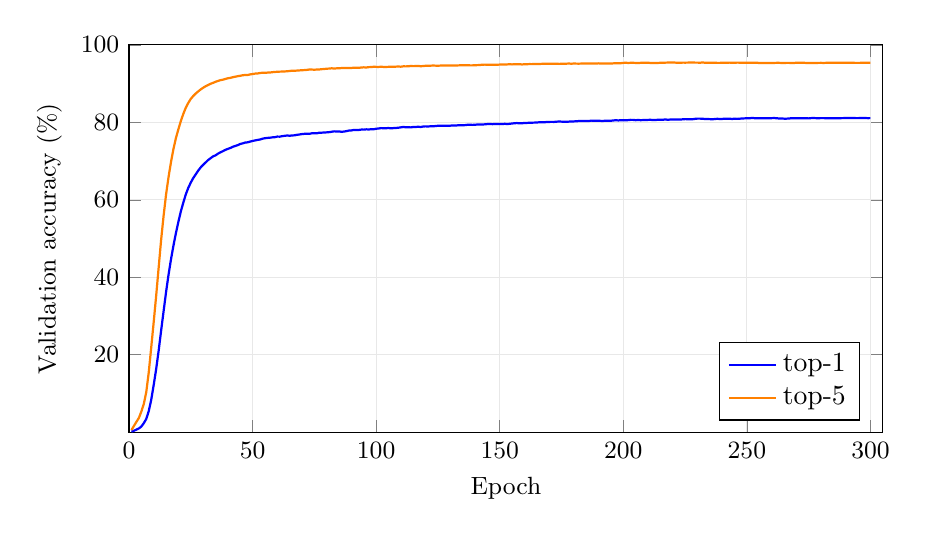
\begin{tikzpicture}
\begin{axis}[
    width=0.92\linewidth, height=6.5cm,
    xlabel={Epoch}, ylabel={Validation accuracy (\%)},
    xmin=0, xmax=305, ymin=0, ymax=100,
    xtick={0,50,100,150,200,250,300}, ytick={20,40,60,80,100},
    legend pos=south east, legend cell align={left},
    grid=major, grid style={gray!18},
    tick label style={font=\small}, label style={font=\small},
    every axis plot/.append style={line width=0.8pt, mark=none},
]
\addplot[blue] coordinates {
(1,0.13) (2,0.38) (3,0.66) (4,0.97) (5,1.46) (6,2.34) (7,3.43) (8,5.45) (9,8.35) (10,12.18) (11,16.31) (12,21.01) (13,26.20) (14,31.21) (15,36.16) (16,40.63) (17,44.65) (18,48.20) (19,51.42) (20,54.36) (21,57.05) (22,59.32) (23,61.42) (24,63.10) (25,64.45) (26,65.62) (27,66.57) (28,67.53) (29,68.37) (30,69.04) (31,69.65) (32,70.26) (33,70.74) (34,71.22) (35,71.47) (36,71.92) (37,72.26) (38,72.56) (39,72.90) (40,73.15) (41,73.39) (42,73.70) (43,73.90) (44,74.12) (45,74.42) (46,74.58) (47,74.78) (48,74.85) (49,75.03) (50,75.21) (51,75.33) (52,75.47) (53,75.57) (54,75.78) (55,75.91) (56,75.99) (57,76.04) (58,76.13) (59,76.17) (60,76.33) (61,76.31) (62,76.44) (63,76.53) (64,76.61) (65,76.55) (66,76.62) (67,76.66) (68,76.79) (69,76.87) (70,76.98) (71,77.04) (72,77.09) (73,77.03) (74,77.19) (75,77.22) (76,77.17) (77,77.34) (78,77.34) (79,77.39) (80,77.42) (81,77.48) (82,77.58) (83,77.68) (84,77.65) (85,77.66) (86,77.57) (87,77.63) (88,77.74) (89,77.89) (90,77.92) (91,78.06) (92,78.02) (93,78.04) (94,78.14) (95,78.13) (96,78.20) (97,78.17) (98,78.23) (99,78.21) (100,78.36) (101,78.42) (102,78.52) (103,78.49) (104,78.49) (105,78.54) (106,78.46) (107,78.52) (108,78.56) (109,78.62) (110,78.72) (111,78.81) (112,78.74) (113,78.72) (114,78.71) (115,78.81) (116,78.81) (117,78.88) (118,78.80) (119,78.93) (120,78.97) (121,78.94) (122,78.99) (123,78.97) (124,79.06) (125,79.12) (126,79.14) (127,79.14) (128,79.14) (129,79.13) (130,79.15) (131,79.22) (132,79.17) (133,79.24) (134,79.24) (135,79.26) (136,79.29) (137,79.38) (138,79.40) (139,79.35) (140,79.39) (141,79.45) (142,79.44) (143,79.45) (144,79.50) (145,79.56) (146,79.59) (147,79.54) (148,79.59) (149,79.59) (150,79.60) (151,79.57) (152,79.63) (153,79.58) (154,79.63) (155,79.71) (156,79.78) (157,79.82) (158,79.75) (159,79.76) (160,79.86) (161,79.86) (162,79.90) (163,79.92) (164,79.94) (165,79.98) (166,80.02) (167,80.02) (168,80.01) (169,80.11) (170,80.12) (171,80.13) (172,80.12) (173,80.18) (174,80.22) (175,80.19) (176,80.15) (177,80.18) (178,80.19) (179,80.25) (180,80.25) (181,80.29) (182,80.34) (183,80.38) (184,80.36) (185,80.35) (186,80.34) (187,80.45) (188,80.43) (189,80.42) (190,80.42) (191,80.38) (192,80.38) (193,80.45) (194,80.41) (195,80.42) (196,80.50) (197,80.55) (198,80.50) (199,80.56) (200,80.55) (201,80.55) (202,80.58) (203,80.65) (204,80.64) (205,80.57) (206,80.61) (207,80.57) (208,80.59) (209,80.59) (210,80.64) (211,80.67) (212,80.59) (213,80.61) (214,80.68) (215,80.70) (216,80.67) (217,80.76) (218,80.66) (219,80.73) (220,80.73) (221,80.73) (222,80.75) (223,80.72) (224,80.79) (225,80.84) (226,80.82) (227,80.82) (228,80.81) (229,80.91) (230,80.97) (231,80.97) (232,80.94) (233,80.87) (234,80.86) (235,80.84) (236,80.80) (237,80.87) (238,80.92) (239,80.88) (240,80.89) (241,80.95) (242,80.91) (243,80.95) (244,80.88) (245,80.95) (246,80.90) (247,80.94) (248,81.01) (249,81.03) (250,81.07) (251,81.04) (252,81.15) (253,81.09) (254,81.07) (255,81.09) (256,81.06) (257,81.06) (258,81.08) (259,81.06) (260,81.09) (261,81.12) (262,81.07) (263,81.01) (264,81.02) (265,80.96) (266,80.96) (267,80.99) (268,81.08) (269,81.06) (270,81.08) (271,81.09) (272,81.07) (273,81.04) (274,81.06) (275,81.03) (276,81.10) (277,81.12) (278,81.09) (279,81.08) (280,81.10) (281,81.10) (282,81.08) (283,81.07) (284,81.06) (285,81.05) (286,81.08) (287,81.08) (288,81.09) (289,81.10) (290,81.13) (291,81.12) (292,81.11) (293,81.13) (294,81.10) (295,81.10) (296,81.11) (297,81.11) (298,81.11) (299,81.09) (300,81.10)
};
\addlegendentry{top-1}
\addplot[orange] coordinates {
(1,0.56) (2,1.62) (3,2.66) (4,3.67) (5,5.34) (6,7.29) (7,10.38) (8,15.46) (9,21.89) (10,28.42) (11,35.22) (12,42.44) (13,49.62) (14,55.84) (15,61.36) (16,65.86) (17,69.77) (18,73.15) (19,75.97) (20,78.25) (21,80.38) (22,82.22) (23,83.80) (24,85.03) (25,86.06) (26,86.80) (27,87.44) (28,87.99) (29,88.50) (30,88.94) (31,89.33) (32,89.64) (33,89.96) (34,90.20) (35,90.47) (36,90.69) (37,90.90) (38,91.02) (39,91.21) (40,91.39) (41,91.49) (42,91.66) (43,91.79) (44,91.92) (45,92.03) (46,92.16) (47,92.24) (48,92.23) (49,92.38) (50,92.48) (51,92.59) (52,92.62) (53,92.75) (54,92.81) (55,92.79) (56,92.85) (57,92.87) (58,92.96) (59,93.02) (60,93.06) (61,93.10) (62,93.12) (63,93.15) (64,93.20) (65,93.26) (66,93.35) (67,93.34) (68,93.37) (69,93.42) (70,93.47) (71,93.50) (72,93.56) (73,93.65) (74,93.63) (75,93.60) (76,93.64) (77,93.66) (78,93.74) (79,93.78) (80,93.86) (81,93.89) (82,93.96) (83,93.91) (84,93.95) (85,93.98) (86,94.02) (87,94.04) (88,94.03) (89,94.06) (90,94.05) (91,94.12) (92,94.09) (93,94.08) (94,94.17) (95,94.21) (96,94.17) (97,94.26) (98,94.29) (99,94.35) (100,94.33) (101,94.32) (102,94.36) (103,94.32) (104,94.31) (105,94.34) (106,94.35) (107,94.34) (108,94.39) (109,94.42) (110,94.38) (111,94.47) (112,94.46) (113,94.48) (114,94.56) (115,94.52) (116,94.54) (117,94.57) (118,94.50) (119,94.54) (120,94.61) (121,94.63) (122,94.64) (123,94.67) (124,94.65) (125,94.63) (126,94.66) (127,94.70) (128,94.69) (129,94.70) (130,94.71) (131,94.66) (132,94.68) (133,94.71) (134,94.73) (135,94.75) (136,94.76) (137,94.75) (138,94.72) (139,94.72) (140,94.77) (141,94.78) (142,94.82) (143,94.89) (144,94.91) (145,94.89) (146,94.89) (147,94.88) (148,94.87) (149,94.89) (150,94.92) (151,94.92) (152,94.95) (153,94.97) (154,95.00) (155,94.97) (156,95.01) (157,94.99) (158,95.01) (159,94.96) (160,95.00) (161,95.02) (162,95.05) (163,95.04) (164,95.10) (165,95.06) (166,95.08) (167,95.11) (168,95.14) (169,95.11) (170,95.12) (171,95.13) (172,95.16) (173,95.16) (174,95.10) (175,95.13) (176,95.14) (177,95.16) (178,95.19) (179,95.15) (180,95.19) (181,95.17) (182,95.16) (183,95.18) (184,95.20) (185,95.21) (186,95.23) (187,95.20) (188,95.23) (189,95.19) (190,95.24) (191,95.19) (192,95.20) (193,95.23) (194,95.22) (195,95.20) (196,95.24) (197,95.29) (198,95.28) (199,95.28) (200,95.36) (201,95.40) (202,95.34) (203,95.38) (204,95.38) (205,95.35) (206,95.33) (207,95.37) (208,95.41) (209,95.41) (210,95.40) (211,95.34) (212,95.33) (213,95.32) (214,95.35) (215,95.38) (216,95.39) (217,95.42) (218,95.44) (219,95.46) (220,95.46) (221,95.43) (222,95.39) (223,95.38) (224,95.43) (225,95.42) (226,95.43) (227,95.45) (228,95.49) (229,95.43) (230,95.43) (231,95.40) (232,95.46) (233,95.41) (234,95.38) (235,95.41) (236,95.42) (237,95.41) (238,95.36) (239,95.36) (240,95.40) (241,95.40) (242,95.40) (243,95.43) (244,95.38) (245,95.39) (246,95.43) (247,95.42) (248,95.41) (249,95.41) (250,95.41) (251,95.38) (252,95.39) (253,95.41) (254,95.41) (255,95.32) (256,95.33) (257,95.33) (258,95.35) (259,95.34) (260,95.34) (261,95.35) (262,95.37) (263,95.37) (264,95.35) (265,95.35) (266,95.36) (267,95.36) (268,95.35) (269,95.34) (270,95.39) (271,95.39) (272,95.37) (273,95.39) (274,95.34) (275,95.34) (276,95.34) (277,95.33) (278,95.35) (279,95.36) (280,95.37) (281,95.35) (282,95.37) (283,95.37) (284,95.38) (285,95.39) (286,95.39) (287,95.38) (288,95.38) (289,95.37) (290,95.38) (291,95.37) (292,95.37) (293,95.38) (294,95.36) (295,95.36) (296,95.37) (297,95.37) (298,95.37) (299,95.37) (300,95.37)
};
\addlegendentry{top-5}
\end{axis}
\end{tikzpicture}
\end{center}

\noindent ConvNeXt-T / ImageNet-1k validation accuracy per epoch over the
full 300-epoch schedule (bf16, 4$\times$ 4060 Ti). Top-1 climbs to
$81.10\%$ and top-5 to $95.37\%$ with no late-schedule plateau or
overfitting dip. The nine 30-minute thermal rests are invisible, each
resuming bit-for-bit.

\subsection*{Phase 4: the verified trainer}
\label{sec:convnext_phase4}

Everything above this point is the phase-2 Lean$\to$JAX trainer. The
phase-4 peer, which trains the same network through the proof-rendered
StableHLO that \S\ref{sec:convnext_runit} ran at Imagenette scale,
exists and builds. It is
\texttt{apps/imagenette/MainConvNeXtImagenet.lean}, built as
\texttt{lake build convnext-imagenet-verified}:

\begin{verbatim}
-- Identical backbone, 1000 classes instead of 10.
def convnextImagenetVerified : VerifiedNetSpec where
  name       := "ConvNeXt-T (ImageNet-1k)"
  slug       := "convnextin"
  nClasses   := 1000
  data       := .imagenet
  shimScript := "generated_convnext_tiny_imagenet_shim.py"
  layers     := [ ... the Imagenette stack, 1000-class head ... ]

-- 300 epochs, because that is the schedule the phase-2 number
-- above was measured on. Batch is 32 PER DEVICE.
def convnextImagenetConfig : VerifiedConfig where
  epochs    := 300
  batchSize := 32
\end{verbatim}

\noindent The head is the only parameter shape that moves, from
$768 \times 10$ to $768 \times 1000$, which takes the count from
27,826,282 to \textbf{28,587,592}. Three kernel \texttt{\#guard}s hold
the two specs together at everything else: equal
\texttt{toSpecs.size}, equal \texttt{toSpecs.pop.pop}, and a
\texttt{back!} of \texttt{(\#[1000], 2)}.

\medskip\noindent\textbf{The collectives are gated by two gates, and
they prove different things.}
\texttt{tests/TestConvNeXtDpCheck.lean} pins the data-parallel forward
bit-exactly against its single-device peer. That gate hands both
replicas the same rows, so it is structurally blind to a shard-offset
bug, and \texttt{tests/TestConvNeXtShardCheck.lean} closes exactly that
hole by giving the replicas genuinely different data. ConvNeXt is where
the shard check was written before being generalized to the other nets,
so this is the one chapter where both gates are native rather than
inherited.

\medskip\noindent\textbf{Four of the paper's six extra knobs are
rendered, and one combination is missing.} Weight-decay exclusion, grad
clipping and stochastic depth are render variants, spelled \texttt{wx},
\texttt{clip} and \texttt{drop}, and
\texttt{convnextin\_adamdpwxclipdrop} carries all three at once on top
of AdamW and the four-way all-reduce. EMA is a render variant too
(\texttt{convnextin\_emadp}), but no committed artifact combines it with
the other three, so there is no single graph carrying the whole
regularizer stack. Mixup and CutMix never enter the graph at all,
because they are data-side and ride the shim.

\medskip\noindent\textbf{What it has not done is run.} No phase-4
ImageNet result exists for this network, which is why every accuracy
above comes from phase 2. What is measured is the throughput, and the
schedule follows from it:

\begin{center}
\begin{tabular}{l r r r r}
\hline
Box & ms/step & min/epoch & 300 epochs & Val top-1 \\
\hline
4$\times$ 4060 Ti (CUDA)  & 184 & 30.7 & $\sim$156.6 h (6.5 d) & TBD \\
4$\times$ 3060 (CUDA)     & 161 & 26.9 & $\sim$137.4 h (5.7 d) & TBD \\
\hline
\end{tabular}
\end{center}

\noindent That is 10,009 steps per epoch, against the reference's 5,004.
\textbf{One thing differs between this row and the phase-2 rows, and it is
not the network}: the verified render's batch is 32 per device, so four
replicas give a global 128 against phase 2's 256. Both still see the same
1.28M images per epoch, which is why the minutes-per-epoch column compares
even though the step counts do not. The batch is 32 because \texttt{cBS}
is still a private constant in the renderer while \texttt{nClasses} became
a parameter, which is a refactor rather than a limit. Precision no longer
differs --- the verified renders gained a bf16 arm and the row above is
measured on it --- so the remaining gap, about $2\times$ per epoch, is the
lowerer.

\noindent\textbf{[TODO: run \texttt{convnext-imagenet-verified}.]}

\subsection*{What the ConvNeXt recipe changes from the 2018 recipe}

The ResNet-34 trainer of Chapter~\ref{chap:residual} is the
\emph{2018-era} recipe: the original paper's SGD-with-momentum plus
the ``bag of tricks'' polish (cosine schedule, warmup, label
smoothing, random-resized-crop). The config above is the \emph{2022}
ConvNeXt recipe, DeiT's transformer-training playbook applied to a
convnet. Where Chapter~\ref{chap:residual}'s RSB-A3 side quest showed
the 2018$\to$2021 jump on a \emph{fixed} ResNet, this table shows the
2018$\to$2022 jump with the block modernized in step. Since
``the recipe is the thesis'' is this architecture's whole argument,
the diff below is the chapter in table form. The
\texttt{trainAdamSched} entry point is identical in both columns, and
every row is a one-line change to the \texttt{VerifiedNetSpec}, the
\texttt{VerifiedConfig}, or the arguments beside them:

\begin{center}
\begin{tabular}{@{}l p{2.9cm} p{3.2cm} p{6.3cm}@{}}
\hline
Knob & ResNet-34 (2018) & ConvNeXt-T (2022) & What the ConvNeXt choice buys \\
\hline
Backbone      & basic block, 21.8\,M   & ConvNeXt block, 28.6\,M       & BN+ReLU $\to$ LN+GELU; dw-$7\times7$ + inverted bottleneck + LayerScale --- the modernized block this chapter built \\
Optimizer     & SGD + momentum $0.9$   & AdamW                         & decoupled decay + per-parameter step scale; LR-robust where B0's RMSProp proved fragile \\
Peak LR       & $0.1$                  & $2.5\mathrm{e}{-4}$           & linearly scaled from the official $4\mathrm{e}{-3}$@4096 --- AdamW's scale, not comparable to SGD's $0.1$ \\
Warmup        & 5 epochs               & 20 epochs                     & heavy augmentation + adaptive optimizer want a long, gentle ramp \\
Epochs        & 90                     & 300                           & heavy regularization needs a long schedule to pay, and converts it straight into accuracy rather than into overfitting \\
Loss          & softmax cross-entropy  & CE over soft targets          & unlike A3's BCE switch, ConvNeXt keeps CE --- the softening comes from the Mixup/CutMix labels \\
Weight decay  & $10^{-4}$, all params  & $0.05$, skip 1-D params       & $500\times$ stronger, never on norm/bias/LayerScale (timm's \texttt{no\_weight\_decay}) \\
Augmentation  & RRC + hflip            & full DeiT pack                & RandAugment + Mixup + CutMix + Random Erasing --- where the modernization actually lives \\
Stochastic depth & none                & drop-path $0.1$               & randomly drops whole residual branches per step --- the depth regularizer \\
EMA           & none                   & decay $0.9999$                & evaluates a smoothed shadow of the weights; with drop-path, together ${<}5\%$ per epoch \\
Grad clip     & none                   & global-norm $1.0$             & cheap insurance that made the peak LR a non-event \\
\hline
\end{tabular}
\end{center}

\noindent What carries over unchanged: cosine LR decay, the
warmup-then-anneal structure, random-resized-crop + horizontal flip
as the base augmentation, label smoothing $0.1$, batch 256, train
and eval both at $224$ (no FixRes), and bf16 matmul and convolution.

The augmentation row is the full DeiT pack: Mixup (Zhang et al.\ 2017,
\href{https://arxiv.org/abs/1710.09412}{arXiv:1710.09412}), CutMix
(Yun et al.\ 2019, \href{https://arxiv.org/abs/1905.04899}{arXiv:1905.04899}),
Random Erasing (Zhong et al.\ 2017,
\href{https://arxiv.org/abs/1708.04896}{arXiv:1708.04896}), and
RandAugment (Cubuk et al.\ 2019,
\href{https://arxiv.org/abs/1909.13719}{arXiv:1909.13719}). All four
are implemented as data-only kernels that mutate the input tensor
before the graph sees it, tier 1 in our codegen scope, no MLIR
plumbing required. Mixup and CutMix route through a soft-label
train-step variant since they produce fractional labels. Random
Erasing and RandAugment leave labels alone.

The through-line is the same \emph{regularize harder, train bigger}
as RSB-A3, arrived at from the transformer side: keep cross-entropy
and soften the targets instead of switching losses, AdamW instead of
LAMB (the batch stays moderate), stochastic depth and EMA from the
ViT toolkit, and a $3\times$ longer schedule to let the
regularization pay.

\section{Side quest: ConvNeXt-S and ConvNeXt-B}
\label{sec:convnext_sb}

Scaling ConvNeXt-T is two moves. \textbf{S} deepens stage 3 from 9 blocks to 27
and touches nothing else; \textbf{B} does that \emph{and} widens every stage,
$96/192/384/768 \to 128/256/512/1024$. On the JAX side both are parameter edits.
On the verified side they are not the same job at all.

\begin{center}
\begin{tabular}{@{}l c c r@{}}
\hline
model & params & renderer work & one card, bs32: fp32 $\to$ bf16 \\
\hline
ConvNeXt-T & $28.6$\,M        & ---                 & $157.9 \to 121.1$\,ms \;($1.30\times$) \\
ConvNeXt-S & $50{,}222{,}152$ & \textbf{none}       & $268.4 \to 192.7$\,ms \;($\mathbf{1.39\times}$) \\
ConvNeXt-B & $88{,}589{,}416$ & ${\sim}27$ literals & $395.7 \to 294.3$\,ms \;($1.34\times$) \\
\hline
\end{tabular}
\end{center}

\noindent Counts are \texttt{\#guard}ed against $50.22$\,M and $88.59$\,M.
\textbf{Renderer cost tracks how many dimensions move, not how many parameters}
--- depth is already a loop, so S is free, while B's widening costs twenty-seven
threaded literals. Those step figures are the \emph{graph's}; T and B ran as
controls and returned their committed $157.8$ and $396.0$\,ms, which is what
makes S's $1.39\times$ a measurement. S being fastest is not what ``deeper costs
more'' predicts: depth adds blocks at widths bf16 already suits.

\medskip\noindent \textbf{A full schedule}, on four cards at global batch $128$
--- $10{,}009$ steps per epoch, double every other net here, which is what the
$300$-epoch schedule really pays for. Totals include $37.5$\,s per epoch of
evaluation and checkpointing.

\begin{center}
\begin{tabular}{@{}l r r r@{}}
\hline
verified, 4 cards & ms/step & min/epoch & 300 epochs \\
\hline
ConvNeXt-T & $217 \to 184$ & $36.2 \to 30.7$ & $184 \to 157$\,h \;($7.7 \to 6.5$\,d) \\
ConvNeXt-S & $366 \to 292$ & $61.0 \to 48.8$ & $308 \to 247$\,h \;($12.8 \to 10.3$\,d) \\
ConvNeXt-B & $534 \to 446$ & $89.1 \to 74.4$ & $449 \to 375$\,h \;($18.7 \to 15.6$\,d) \\
\hline
\end{tabular}
\end{center}

\noindent \textbf{T and B are measured; S is derived} --- the trainer costs a
near-constant multiple of the graph ($1.37\times$/$1.35\times$ fp32,
$1.519\times$/$1.516\times$ bf16), and applying those reproduces T's and B's
published totals to within $0.5$\,h. A direct probe of S afterwards returned
$368 \to 301$\,ms against the $366 \to 292$ derived here, so the model holds on
this net --- \S\ref{sec:vit_sb} is where it does not, and says why. Note how much of bf16 the trainer eats: a
$1.39\times$ graph is a $1.25\times$ run, because the shim feed and the
all-reduce do not get faster. The phase-2 peers, at twice the batch and so half
the steps, take $71.6$, $108.8$ and $166.5$ hours compute-only --- so the
${\sim}2\times$ gap is the batch, not the lowerer.

\medskip\noindent \textbf{Status: rendered, not trained.} Artifacts emit, shapes
tie, counts are guarded, a few steps run under each size. No accuracy, and the
numeric ties against the JAX peers have not been run.

\chapter{Vision Transformer}
\label{chap:attention}

\prosesection{Where Part 1 has been heading}

Every previous chapter has introduced a new architectural primitive
and proved its backward pass. Each one slotted into the
\texttt{VerifiedNetSpec} type and earned its own \texttt{has\_vjp}
theorem, and that includes convolution, BatchNorm, residual,
depthwise, SE, LayerNorm and GELU.
This chapter does the same for attention, but it also does
something larger: it composes \emph{every} layer the framework has
proved so far into one machine-checked backward pass over a
complete state-of-the-art image classifier.

The destination is Theorem~\ref{thm:vit_body_has_vjp_mat} at the
end of the chapter. It says, roughly: the full ViT backbone is a
\(\HasVJPMat\), and that backbone is the patch embedding, twelve
transformer blocks and a final LayerNorm. The proof composes everything
this chapter introduces, plus most of what the previous chapters
introduced, into a single tower of \texttt{vjpMat\_comp}
applications. Read the proof's dependency list and you see a tour
of Part 1: dense, residual, layer norm, GELU, softmax, matrix
multiply, plus the eight or ten matrix-machinery lemmas this
chapter sets up. None of them is new in its own right. What's new
is how high the composition rule can be pushed.

\section{Run it first}
\label{sec:vit_runit}

Before any of the attention mathematics, train the network that needs
it. Four commands, and the last network in Part 1 is also the quickest
one in it:

\begin{verbatim}
lake exe cache get                        # Mathlib oleans, ~30 s
./download_imagenette.sh                  # 330 MB dl, 2.4 GB unpacked
lake build vit-verified-adam
./.lake/build/bin/vit-verified-adam data
\end{verbatim}

On one RTX 4060 Ti (CUDA 12.9), from
\texttt{runs/2026-08-12-vit-imagenette-xla-cuda/}. XLA's startup banner
is removed, the network description line is wrapped, the per-step lines
are dropped, and the middle of the run is elided:

\begin{verbatim}
[pjrt_ffi] XLA backend: PJRT 0.112, 1 device(s)
[pjrt_ffi] compiled verified_mlir/vit_adam_train_step.mlir
             (@vit_adam_train_step, 603 outputs, 1 replica)
             in 6104 ms
[pjrt_ffi] compiled verified_mlir/vit_fwd.mlir
             (@vit_fwd, 1 outputs, 1 replica) in 1644 ms
ViT-Tiny on Imagenette 224² (patch-16 → CLS+pos → 12 transformer
  blocks @ dim192/3heads/MLP768 → final LN → CLS-head 10)
  via the VERIFIED renderer → XLA/PJRT → GPU
  train 9469, val 3925; bs 32, ViT-Tiny adam
    (cosine+warmup 5ep, baseLR 0.000300), He init
[pjrt_ffi] RESIDENT: @vit_adam_train_step holds 600 parameter
             tensors (63.2 MB) on 1 device; they stop crossing PCIe
             from here
Epoch 1/80: loss=2.127541 lr=0.000060
  epoch 1: val_acc = 1381/3925 = 35.184713%  top5 = 3121/3925 = 79.515924%
Epoch 2/80: loss=1.869707 lr=0.000120
  epoch 2: val_acc = 1619/3925 = 41.248408%  top5 = 3350/3925 = 85.350318%
Epoch 3/80: loss=1.750333 lr=0.000180
  epoch 3: val_acc = 1591/3925 = 40.535032%  top5 = 3362/3925 = 85.656051%
Epoch 30/80: loss=1.004060 lr=0.000225
  epoch 30: val_acc = 2571/3925 = 65.503185%  top5 = 3698/3925 = 94.216561%
Epoch 79/80: loss=0.515797 lr=0.000000
  epoch 79: val_acc = 2698/3925 = 68.738854%  top5 = 3551/3925 = 90.471338%
Epoch 80/80: loss=0.515159 lr=0.000000
  epoch 80: val_acc = 2698/3925 = 68.738854%  top5 = 3549/3925 = 90.420382%
done (trained ViT-Tiny adam + cosine/warmup via packed threading).
\end{verbatim}

Eighty epochs at about 18 seconds each, twenty-four minutes in total,
and \textbf{68.74\%} top-1 with \textbf{90.42\%} top-5 on Imagenette's
3,925-image validation split. The best epoch reached $68.92\%$. That is
the fastest network in this book's Imagenette column by a wide margin
and also the least accurate one in it, and
\S\ref{sec:attention_vit_example} is about why both halves of that
sentence are the same fact.

\medskip\noindent\textbf{Two compile lines, and the second one is the
whole eval story.} Like ConvNeXt and unlike the three BatchNorm
chapters, ViT emits no \texttt{vit\_fwd\_eval}. LayerNorm computes its
statistics from the activation in front of it every time, so there is
nothing to freeze and the training forward and the evaluation forward
are the same function.

\medskip\noindent\textbf{The top-5 column goes the wrong way, and that
is the chapter's result in miniature.} Top-1 climbs the whole run, 35.2
to 68.7. Top-5 climbs to $94.88\%$ at epoch 25 and then \emph{falls},
finishing 4.5 points down at $90.42\%$. On a ten-class problem top-5 is
a weak question, so what that divergence measures is a network growing
more confident about its top choice while its ranking of the remaining
classes decays. A transformer with 5.5M parameters and 9,469 training
images has enough capacity to memorize its way to a better top-1 and
not enough signal to keep the tail honest, which is
\S\ref{sec:attention_vit_example}'s data-hunger argument showing up
inside a single run rather than across the comparison table.

Attention is where you would expect this to break. That run did not
execute a
reimplementation of the network this chapter describes. It executed
\texttt{verified\_mlir/vit\_adam\_train\_step.mlir}, which is
\texttt{pretty(provenGraph)} off the renderer. Every softmax in it
backpropagates by Theorem~\ref{thm:softmax_has_vjp}, every scaled
dot-product attention by \S\S\ref{thm:sdpa_back_Q_correct}--%
\ref{thm:sdpa_back_V_correct}, every LayerNorm by
Chapter~\ref{chap:layernorm}'s, every GELU by that chapter's, and every
residual skip by Chapter~\ref{chap:residual}'s additive fan-in.

\medskip\noindent\textbf{And the fold holds at every depth.}
\texttt{vitForward2\_has\_vjp} chains the patch embedding, all
\emph{twelve} transformer blocks, the final LayerNorm and the head
through \texttt{vjp\_comp}, with \texttt{vitForward2\_has\_vjp\_correct}
carrying it back to the forward the spec denotes, and
\texttt{vitForwardKV\_has\_vjp} generalizes it to depth $k$. Its only
hypothesis is $\varepsilon > 0$ at the LayerNorms. It is a single global
\texttt{HasVJP} over the entire network for the same reason
Chapter~\ref{chap:layernorm}'s is --- softmax, GELU and LayerNorm are all
smooth --- so ViT gets the strong sentence too: every operation in the
graph that just trained carries a proved backward, and their
composition into the whole network carries one too.

\prosesection{Attention in one equation}

A transformer encoder block does two things to its input sequence
\(X \in \mathbb{R}^{N \times d}\) (think of \(N\) image patches,
each represented as a \(d\)-vector):

\begin{enumerate}
\item \textbf{Multi-head self-attention} (MHSA): each output row
  is a weighted average of \emph{all} input rows, where the weights
  are computed from the input itself.
\item \textbf{Per-token MLP}: a small two-layer MLP applied
  independently to every row.
\end{enumerate}

Both halves are wrapped in a LayerNorm + residual sandwich
(exactly the same template as ConvNeXt's blocks from
Chapter~\ref{chap:layernorm}, and the layout that transferred to
convnets in 2022 actually came from transformers in 2017).

The interesting half is the first one. \emph{Scaled dot-product
attention} computes, for queries \(Q\), keys \(K\), and values
\(V\) (all linear projections of \(X\)):

\[
\mathrm{Attention}(Q, K, V) \;=\; \mathrm{softmax}\!\left(\frac{Q K^\top}{\sqrt{d_h}}\right) V.
\]

In words: every row of \(Q\) is compared to every row of \(K\) via
inner product (the \(QK^\top\) matrix is \(N \times N\), one
entry per query-key pair). Each row of that \(N \times N\) matrix
is passed through softmax to get a probability distribution over
the keys (which positions to attend to). Those probabilities then
weight the rows of \(V\) to produce the output. The
\(1 / \sqrt{d_h}\) scaling keeps the softmax from saturating at
large \(d_h\). \emph{Multi-head} attention just runs several copies
of this in parallel on lower-dimensional projections, concatenating
the outputs.

Each token, meaning each row of \(X\), ends up looking at every
other token. That's the qualitative break from CNNs:
convolutions look only at a local neighborhood, attention looks
everywhere. The receptive field is global from the first layer.

\prosesection{Why this chapter has thirty theorems}

The math of attention is matrix algebra. Chapter~\ref{chap:tensor}'s
foundation rules (chain, sum, product, identity) were stated and
proved for \emph{vector} functions. Before we can prove backward
passes through \(Q K^\top\) and the row-wise softmax, we need the
matrix-level lifts of those rules: chain rule on matrices,
additive fan-in on matrices, identity on matrices, plus matrix-specific
moves like transpose, matmul-with-one-factor-fixed, and scalar
scale. That's the first section of theorems below
(\textbf{Matrix-level machinery}, \(\sim\)15 theorems). Every one of them
is a mechanical lift of a vector-level theorem from
Chapter~\ref{chap:tensor}, proved via the row-projection
\(\mathrm{ContinuousLinearMap}\) and the existing chain rule. Pay
the cost once, reuse forever.

The second section (\textbf{Attention proofs}, \(\sim\)15 theorems)
applies the matrix machinery to the actual attention math. Row-wise
softmax (a per-row softmax applied to the \(N \times N\) score
matrix) has the well-known closed-form Jacobian \(p_i(\delta_{ij}
- p_i)\), and we prove the row-wise lifting that says this holds
across matrices. Scaled dot-product attention's backward decomposes
into three matmul-backward applications (one for each of \(Q\),
\(K\), \(V\)) plus the row-wise softmax backward, and we prove each. Then
multi-head, then the attention sublayer (with residual), then the
MLP sublayer (with residual), then a single transformer block,
then a \(k\)-deep transformer tower, then the full ViT body. Each
step is one or two compositions of the previous step. The chain
that started at \texttt{vjp\_comp} in Chapter~\ref{chap:tensor}
reaches all the way to a 5.5M-parameter image classifier here.

\prosesection{What's actually proved}

That's the framework-side payoff of this chapter: \textbf{every
architectural piece used by any Part-1 network has a machine-checked
backward}. Once we land Theorem~\ref{thm:vit_body_has_vjp_mat}, the
sentence ``the gradient computed by this trainer is the
mathematically correct one'' is no longer a hope or a folklore
result. It is a theorem the Lean kernel verifies on every
build.

The empirical-side payoff comes after the theorems, in the Example
section: ViT-Tiny trained on Imagenette underperforms the
ConvNets, fairly dramatically, because 9{,}469 training images is
too small for a transformer's lack of inductive bias. That's
informative on its own terms: the data-hungry-transformer story
made concrete.

\section{Matrix-level machinery}
\label{sec:matrix_machinery}

Attention is fundamentally matrix algebra: queries times keys
transposed (\(QK^T\)), softmax over rows of the resulting matrix,
matmul against values (\(\cdot V\)). Before we can prove backward
passes through these operations, we need the matrix-level
extensions of Ch~\ref{chap:tensor}'s foundation rules. Each theorem
below is the matrix lift of a vector-level theorem from Ch
\ref{chap:tensor}, proved by composing the vector version with the
row-projection \(\mathrm{ContinuousLinearMap}\). The Lean proofs all
live in \texttt{Proofs/Tensor.lean} alongside their vector
counterparts. We collect them here because Ch~\ref{chap:attention}
is the first and only chapter to use them.

\begin{definition}[Matrix VJP record]
  \label{def:hasvjpmat}
  \lean{Proofs.HasVJPMat}
  \leanok
  \uses{ax:pdiv, def:hasvjp}
  The rank-2 analogue of Definition~\ref{def:hasvjp}. Define
  \(\pdivMat f\, A\, (i,j)\, (k,l)\) as \(\pdiv\) of the row-major
  flattened map
  \(v \mapsto \mathrm{flatten}\bigl(f(\mathrm{unflatten}\, v)\bigr)\)
  with both index pairs encoded through the
  \((i, j) \leftrightarrow \text{flat}\) bijection. Then
  \(\HasVJPMat\, f\) bundles a backward function \(B\) with: for all
  \(A\), \(dY\), \((i, j)\),
  \[
    B(A, dY)_{ij}
      = \sum_{k, l} \pdivMat f\, A\, (i,j)\, (k,l) \cdot dY_{kl}.
  \]
\end{definition}

\begin{theorem}[Row-independence for matrices]
  \label{ax:pdivMat_rowIndep}
  \lean{Proofs.pdivMat_rowIndep}
  \leanok
  \uses{ax:pdiv, def:hasvjpmat}
  \Assume{}
  \begin{enumerate}
    \item \(g : \Vect{n} \to \Vect{p}\) is differentiable everywhere
          \hfill[\texttt{h\_g\_diff}]
  \end{enumerate}
  \Prove{} applying \(g\) to each row of a matrix has block-diagonal
  Jacobian:
  \(\pdivMat(\text{rowwise } g)\, A\, (i,j)\, (k,l)
    = [i = k] \cdot \pdiv g\, (A_i)\, j\, l\).
\end{theorem}

\begin{proof}
\leanok
\begin{enumerate}
  \item Coordinate factoring: the \((k, l)\) output coordinate of the
    flattened rowwise map is
    \((y \mapsto g(y)_l) \circ \mathrm{rowProj}_k\), where
    \(\mathrm{rowProj}_k\) is the CLM extracting row \(k\) of the
    flat vector.
    \pf{Unfold flatten/unflatten; \(\mathrm{rowProj}_k\) is a
    reindex, hence a CLM.}
  \item Every output coordinate --- hence the whole flat map --- is
    differentiable, so \(\fderiv\) does not fall back to its junk
    default.
    \pf{Assumption 1 composed with the CLM of step 1
    (\texttt{differentiableAt\_pi}).}
  \item \Qed{}
    \pf{Chain rule through the CLM: the derivative of
    \((y \mapsto g(y)_l) \circ \mathrm{rowProj}_k\) at
    \(\basisVec_{(i,j)}\) sees
    \(\mathrm{rowProj}_k(\basisVec_{(i,j)}) = [i = k]\, \basisVec_j\),
    so by Definition~\ref{ax:pdiv} the entry is
    \([i = k] \cdot \pdiv g\,(A_i)\, j\, l\).}
\end{enumerate}
\end{proof}

\begin{theorem}[Matrix-level chain rule]
  \label{thm:vjpMat_comp}
  \lean{Proofs.vjpMat_comp}
  \leanok
  \uses{thm:vjp_comp, ax:pdiv_comp, def:hasvjpmat}
  \Assume{}
  \begin{enumerate}
    \item \(B_F\), \(B_G\) are correct backward functions
          (\(\HasVJPMat\, F\), \(\HasVJPMat\, G\))
          \hfill[\texttt{hF}, \texttt{hG}]
    \item the flattened forms of \(F\) and \(G\) are differentiable
          everywhere \hfill[\texttt{hF\_diff}, \texttt{hG\_diff}]
  \end{enumerate}
  \Prove{} \(\HasVJPMat\, (G \circ F)\).
\end{theorem}

\begin{proof}
\leanok
\emph{Sketch: the VJP chain rule (Theorem~\ref{thm:vjp_comp})
transcribed to rank-2 indices; every step is the same, with double
sums where the rank-1 proof had single sums.}
\begin{enumerate}
  \item Define \(B(A, dY) := B_F\bigl(A,\; B_G(F(A),\, dY)\bigr)\).
  \item \Suffices{} \(B\) matches the \(\pdivMat\) contraction.
    \pf{Definition~\ref{def:hasvjpmat}.}
  \item Chain rule for \(\pdivMat\):
    \(\pdivMat(G \circ F)\, A\, (i,j)\, (k,l)
      = \sum_{p,q} \pdivMat F\, A\, (i,j)\, (p,q) \cdot
        \pdivMat G\, (F A)\, (p,q)\, (k,l)\).
    \pf{The flattened composite is the composite of the flattened
    maps (unflatten \(\circ\) flatten cancels), so the rank-1 chain
    rule (Theorem~\ref{ax:pdiv_comp}) applies at the flat level,
    applicable by assumption 2; re-index the flat middle sum to
    \((p, q)\) pairs.}
  \item \Qed{}
    \pf{Expand the two \texttt{correct} fields in 1, substitute 3,
    and swap the two double sums (pack indices into pairs,
    \texttt{Finset.sum\_comm}, unpack); with 2 this is the goal ---
    step for step the proof of Theorem~\ref{thm:vjp_comp}.}
\end{enumerate}
\end{proof}

\begin{theorem}[Matrix-level additive fan-in]
  \label{thm:biPathMat_has_vjp}
  \lean{Proofs.biPathMat_has_vjp}
  \leanok
  \uses{thm:biPath_has_vjp, ax:pdiv_add, def:hasvjpmat}
  Rank-2 transcription of Theorem~\ref{thm:biPath_has_vjp}: given
  \(\HasVJPMat\) for \(F\) and \(G\) (with flat differentiability),
  \(\HasVJPMat\, (F + G)\) with backward
  \(B_F(A, dY) + B_G(A, dY)\).
\end{theorem}

\begin{proof}
\leanok
\begin{enumerate}
  \item \Suffices{} the summed backward matches the \(\pdivMat\)
    contraction. \pf{Definition~\ref{def:hasvjpmat}.}
  \item \Qed{}
    \pf{Expand both \texttt{correct} fields, merge the double sums
    (\texttt{Finset.sum\_add\_distrib} twice); the sum rule for
    \(\pdivMat\) --- Theorem~\ref{ax:pdiv_add} through the flatten
    bijection --- rewrites
    \(\pdivMat F + \pdivMat G = \pdivMat(F + G)\).}
\end{enumerate}
\end{proof}

\begin{theorem}[Matrix-level identity]
  \label{thm:identityMat_has_vjp}
  \lean{Proofs.identityMat_has_vjp}
  \leanok
  \uses{thm:identity_has_vjp, ax:pdiv_id, def:hasvjpmat}
  \(\HasVJPMat\, (\mathrm{id})\), backward \(B(A, dY) = dY\).
\end{theorem}

\begin{proof}
\leanok
\begin{enumerate}
  \item \(\pdivMat(\mathrm{id})\, A\, (i,j)\, (k,l)
          = [i = k \wedge j = l]\).
    \pf{Flatten \(\circ\) unflatten is the identity on the flat
    vector, so the identity Jacobian (Theorem~\ref{ax:pdiv_id})
    applies; the flat-index equality decodes to
    \(i = k \wedge j = l\) by injectivity of the pairing.}
  \item \Qed{}
    \pf{Contract 1 with \(dY\): the two-dimensional Kronecker sum
    collapses (\texttt{Finset.sum\_eq\_single} twice) to
    \(dY_{ij}\); Definition~\ref{def:hasvjpmat} closes.}
\end{enumerate}
\end{proof}

\begin{theorem}[Scalar-scale Jacobian]
  \label{thm:pdivMat_scalarScale}
  \lean{Proofs.pdivMat_scalarScale}
  \leanok
  \uses{ax:pdiv_mul, ax:pdiv_const, ax:pdiv_id}
  \Prove{} \(\pdivMat(M \mapsto s \cdot M)\, A\, (i,j)\, (k,l)
    = [i = k \wedge j = l] \cdot s\).
\end{theorem}

\begin{proof}
\leanok
\begin{enumerate}
  \item The flattened scalar-scale map reduces to
    \(v \mapsto s \cdot v\).
    \pf{Flatten/unflatten round-trip, pointwise.}
  \item \(\pdiv(v \mapsto s \cdot v) = s \cdot \delta\) at the flat
    indices.
    \pf{Factor as \((\text{const } s) \cdot (\text{identity})\):
    product rule (Theorem~\ref{ax:pdiv_mul}), constant rule
    (Theorem~\ref{ax:pdiv_const}), identity Jacobian
    (Theorem~\ref{ax:pdiv_id}).}
  \item \Qed{}
    \pf{The flat-index equality decodes to
    \(i = k \wedge j = l\) by injectivity of the pairing.}
\end{enumerate}
\end{proof}

\begin{theorem}[Transpose Jacobian]
  \label{thm:pdivMat_transpose}
  \lean{Proofs.pdivMat_transpose}
  \leanok
  \uses{ax:pdiv_reindex}
  \Prove{} \(\pdivMat(\mathrm{transpose})\, A\, (i,j)\, (k,l)
    = [j = k \wedge i = l]\).
\end{theorem}

\begin{proof}
\leanok
\begin{enumerate}
  \item The flattened transpose is a pure gather: at output index
    \(\mathrm{idx}\), it reads \(v\) at the index with components
    swapped.
    \pf{Unfold transpose/flatten/unflatten.}
  \item \Qed{}
    \pf{Reindex Jacobian (Theorem~\ref{ax:pdiv_reindex}) with the
    swap map \(\sigma\): the indicator condition
    \(\mathrm{flat}(i,j) = \mathrm{flat}(l,k)\) decodes to
    \(j = k \wedge i = l\) by injectivity of the pairing.}
\end{enumerate}
\end{proof}

\begin{theorem}[Matmul Jacobian, left factor fixed]
  \label{thm:pdivMat_matmul_left_const}
  \lean{Proofs.pdivMat_matmul_left_const}
  \leanok
  \uses{ax:pdiv_const, ax:pdiv_mul, ax:pdiv_reindex, thm:pdiv_finset_sum}
  \Prove{} \(\pdivMat(B' \mapsto C \cdot B')\, B\, (i,j)\, (k,l)
    = [l = j] \cdot C_{ki}\).
\end{theorem}

\begin{proof}
\leanok
\begin{enumerate}
  \item The flattened map at output index \(\mathrm{idx}\) is
    \(v \mapsto \sum_s C_{k(\mathrm{idx}), s} \cdot
      v_{\mathrm{flat}(s,\, l(\mathrm{idx}))}\) --- a finite sum of
    (constant)\,\(\times\)\,(reindex) terms.
    \pf{Unfold \(\mathrm{Mat.mul}\)/flatten/unflatten.}
  \item Per-index Jacobian: finite-sum rule
    (Theorem~\ref{thm:pdiv_finset_sum}) distributes over \(s\);
    product rule with the \(C\)-factor constant
    (Theorems~\ref{ax:pdiv_mul}, \ref{ax:pdiv_const}) and reindex
    Jacobian (Theorem~\ref{ax:pdiv_reindex}) leave
    \(\sum_s C_{k, s} \cdot [\mathrm{flat}(i,j) = \mathrm{flat}(s, l)]\).
  \item \Qed{}
    \pf{The indicator forces \(s = i\) and \(l = j\) (injectivity of
    the pairing), collapsing the sum to \([l = j] \cdot C_{ki}\).}
\end{enumerate}
\end{proof}

\begin{theorem}[Matmul Jacobian, right factor fixed]
  \label{thm:pdivMat_matmul_right_const}
  \lean{Proofs.pdivMat_matmul_right_const}
  \leanok
  \uses{ax:pdiv_const, ax:pdiv_mul, ax:pdiv_reindex, thm:pdiv_finset_sum}
  \Prove{} \(\pdivMat(A' \mapsto A' \cdot D)\, A\, (i,j)\, (k,l)
    = [i = k] \cdot D_{jl}\).
\end{theorem}

\begin{proof}
\leanok
Mirror image of Theorem~\ref{thm:pdivMat_matmul_left_const}: the
flattened map at output \(\mathrm{idx}\) is
\(v \mapsto \sum_s v_{\mathrm{flat}(k(\mathrm{idx}),\, s)} \cdot
  D_{s,\, l(\mathrm{idx})}\), the same finite-sum-of-reindex-times-constant
shape with the variable factor on the left; the same three steps
(finite-sum, product + constant + reindex rules, indicator collapse
at \(s = j\), \(k = i\)) give \([i = k] \cdot D_{jl}\).
\end{proof}

\begin{theorem}[Matmul VJP, left factor fixed]
  \label{thm:matmul_left_const_has_vjp}
  \lean{Proofs.matmul_left_const_has_vjp}
  \leanok
  \uses{thm:pdivMat_matmul_left_const, def:hasvjpmat}
  \(\HasVJPMat\, (B' \mapsto C \cdot B')\), backward
  \(dB = C^{T} \cdot dY\).
\end{theorem}

\begin{proof}
\leanok
\begin{enumerate}
  \item Define \(B(B', dY)_{ij} := \sum_k C_{ki}\, dY_{kj}\)
    (that is, \(C^T \cdot dY\)).
  \item \Suffices{} \(B\) matches the \(\pdivMat\) contraction.
    \pf{Definition~\ref{def:hasvjpmat}.}
  \item \Qed{}
    \pf{Substitute the Jacobian
    (Theorem~\ref{thm:pdivMat_matmul_left_const}):
    \(\sum_{k,l} [l = j]\, C_{ki} \cdot dY_{kl}\) collapses at
    \(l = j\) (\texttt{Finset.sum\_ite\_eq'}) to
    \(\sum_k C_{ki}\, dY_{kj} = B\).}
\end{enumerate}
\end{proof}

\begin{theorem}[Matmul VJP, right factor fixed]
  \label{thm:matmul_right_const_has_vjp}
  \lean{Proofs.matmul_right_const_has_vjp}
  \leanok
  \uses{thm:pdivMat_matmul_right_const, def:hasvjpmat}
  \(\HasVJPMat\, (A' \mapsto A' \cdot D)\), backward
  \(dA = dY \cdot D^{T}\).
\end{theorem}

\begin{proof}
\leanok
\begin{enumerate}
  \item Define \(B(A', dY)_{ij} := \sum_l dY_{il}\, D_{jl}\)
    (that is, \(dY \cdot D^T\)).
  \item \Suffices{} \(B\) matches the \(\pdivMat\) contraction.
    \pf{Definition~\ref{def:hasvjpmat}.}
  \item \Qed{}
    \pf{Substitute the Jacobian
    (Theorem~\ref{thm:pdivMat_matmul_right_const}):
    \(\sum_{k,l} [i = k]\, D_{jl} \cdot dY_{kl}\) collapses at
    \(k = i\) (\texttt{Finset.sum\_ite\_eq}) to
    \(\sum_l D_{jl}\, dY_{il} = B\).}
\end{enumerate}
\end{proof}

\begin{theorem}[Scalar-scale VJP]
  \label{thm:scalarScale_has_vjp}
  \lean{Proofs.scalarScale_has_vjp}
  \leanok
  \uses{thm:pdivMat_scalarScale, def:hasvjpmat}
  \(\HasVJPMat\, (M \mapsto s \cdot M)\), backward
  \(dA = s \cdot dY\).
\end{theorem}

\begin{proof}
\leanok
By Definition~\ref{def:hasvjpmat} it suffices to contract the
Jacobian (Theorem~\ref{thm:pdivMat_scalarScale}) with \(dY\):
\(\sum_{k,l} [i = k \wedge j = l]\, s \cdot dY_{kl}\) collapses at
\((k, l) = (i, j)\) to \(s \cdot dY_{ij}\). \Qed{}
\end{proof}

\begin{theorem}[Transpose VJP]
  \label{thm:transpose_has_vjp}
  \lean{Proofs.transpose_has_vjp}
  \leanok
  \uses{thm:pdivMat_transpose, def:hasvjpmat}
  \(\HasVJPMat\, (\mathrm{transpose})\), backward
  \(dA = dY^{T}\).
\end{theorem}

\begin{proof}
\leanok
By Definition~\ref{def:hasvjpmat} it suffices to contract the
Jacobian (Theorem~\ref{thm:pdivMat_transpose}) with \(dY\):
\(\sum_{k,l} [j = k \wedge i = l] \cdot dY_{kl}\) collapses at
\((k, l) = (j, i)\) to \(dY_{ji}\). \Qed{}
\end{proof}

\begin{theorem}[Row-wise lifting of any \(\HasVJP\)]
  \label{thm:rowwise_has_vjp_mat}
  \lean{Proofs.rowwise_has_vjp_mat}
  \leanok
  \uses{ax:pdivMat_rowIndep, def:hasvjp, def:hasvjpmat}
  \Assume{}
  \begin{enumerate}
    \item \(B_g\) is a correct backward for
          \(g : \Vect{n} \to \Vect{p}\) (\(\HasVJP\, g\))
          \hfill[\texttt{hg}]
    \item \(g\) is differentiable everywhere \hfill[\texttt{hg\_diff}]
  \end{enumerate}
  \Prove{} \(\HasVJPMat\) of the rowwise map on
  \(\Mat{m}{n} \to \Mat{m}{p}\), with backward applying \(B_g\) to
  each row: \(B(A, dY)_r = B_g(A_r, dY_r)\).
\end{theorem}

\begin{proof}
\leanok
\begin{enumerate}
  \item \Suffices{} \(B\) matches the \(\pdivMat\) contraction.
    \pf{Definition~\ref{def:hasvjpmat}.}
  \item The Jacobian is block-diagonal:
    \(\pdivMat = [i = k] \cdot \pdiv g\, (A_i)\, j\, l\).
    \pf{Row-independence (Theorem~\ref{ax:pdivMat_rowIndep}),
    applicable by assumption 2.}
  \item \Qed{}
    \pf{Contract 2 with \(dY\): the row sum collapses at \(k = i\)
    (\texttt{Finset.sum\_ite\_eq}); what remains is precisely
    \(g\)'s own correctness equation at row \(i\)
    (assumption 1).}
\end{enumerate}
\end{proof}

\begin{theorem}[3D chain rule]
  \label{thm:pdiv3_comp}
  \lean{Proofs.pdiv3_comp}
  \leanok
  \uses{ax:pdiv_comp, def:hasvjp3}
  \Prove{} for flattened-differentiable \(f\), \(g\):
  \(\pdiv_3(g \circ f)\) is the middle-index contraction
  \(\sum_{c_j, h_j, w_j} \pdiv_3 f \cdot \pdiv_3 g\).
\end{theorem}

\begin{proof}
\leanok
\begin{enumerate}
  \item \(\pdiv_3\) is \(\pdiv\) of the flattened map
    (Definition~\ref{def:hasvjp3}), and the flattened composite is
    the composite of the flattened maps.
    \pf{Unflatten \(\circ\) flatten cancels between the stages.}
  \item \Qed{}
    \pf{The rank-1 chain rule (Theorem~\ref{ax:pdiv_comp}) at the
    flat level, then re-index the flat middle sum to
    \((c_j, h_j, w_j)\) triples through the index bijection.}
\end{enumerate}
\end{proof}

\begin{theorem}[3D VJP chain rule]
  \label{thm:vjp3_comp}
  \lean{Proofs.vjp3_comp}
  \leanok
  \uses{thm:pdiv3_comp, thm:vjp_comp, def:hasvjp3}
  Rank-3 transcription of Theorem~\ref{thm:vjp_comp}: composite
  backward \(B(x, dy) = B_f\bigl(x,\, B_g(f\,x,\, dy)\bigr)\).
\end{theorem}

\begin{proof}
\leanok
\begin{enumerate}
  \item \Suffices{} the composite backward matches the \(\pdiv_3\)
    triple-sum contraction. \pf{Definition~\ref{def:hasvjp3}.}
  \item \Qed{}
    \pf{Expand both \texttt{correct} fields, substitute the 3D chain
    rule (Theorem~\ref{thm:pdiv3_comp}), then swap the two triple
    sums by packing each into a product index
    (\texttt{Finset.sum\_product}, \texttt{Finset.sum\_comm}) ---
    the rank-3 rendition of Theorem~\ref{thm:vjp_comp} steps 3--6.}
\end{enumerate}
\end{proof}

\begin{theorem}[3D additive fan-in]
  \label{thm:biPath3_has_vjp}
  \lean{Proofs.biPath3_has_vjp}
  \leanok
  \uses{ax:pdiv_add, thm:biPath_has_vjp, def:hasvjp3}
  Rank-3 transcription of Theorem~\ref{thm:biPath_has_vjp}: backward
  is the sum of the two backwards.
\end{theorem}

\begin{proof}
\leanok
By Definition~\ref{def:hasvjp3} it suffices to match the triple-sum
contraction: expand both \texttt{correct} fields, merge the three
nested sums (\texttt{Finset.sum\_add\_distrib} three times), and
apply the sum rule (Theorem~\ref{ax:pdiv_add}, through the flatten
bijection) to rewrite \(\pdiv_3 f + \pdiv_3 g = \pdiv_3(f + g)\).
\Qed{}
\end{proof}

\section{Attention proofs}
\label{sec:attention_proofs}

\begin{theorem}[Softmax Jacobian]
  \label{ax:pdiv_softmax}
  \lean{Proofs.pdiv_softmax}
  \leanok
  \uses{ax:pdiv}
  Writing \(p := \mathrm{softmax}(z)\):
  \Prove{}
  \(\pdiv(\mathrm{softmax})\, z\, i\, j = p_j\, (\delta_{ij} - p_i)\).
\end{theorem}

\begin{proof}
\leanok
\begin{enumerate}
  \item \(\pdiv(\mathrm{softmax})\, z\, i\, j
    = \fderiv_{\R}\,\bigl(z' \mapsto e^{z'_j} \cdot
      (\textstyle\sum_k e^{z'_k})^{-1}\bigr)\, z\, (\basisVec_i)\).
    \pf{Definition~\ref{ax:pdiv}; extract the \(j\)-th coordinate
    (\texttt{fderiv\_apply}), differentiable because the denominator
    \(S := \sum_k e^{z_k}\) is a sum of positive exponentials, hence
    nonzero.}
  \item Differentiate the product: numerator via
    \texttt{HasFDerivAt.exp}, denominator via
    \texttt{(hasDerivAt\_inv).comp\_hasFDerivAt} (licensed by
    \(S > 0\)).
  \item Evaluate at \(\basisVec_i\): the numerator's derivative
    contributes \(e^{z_j}\, \delta_{ji}\), and the denominator's
    contributes \(-e^{z_j}\, S^{-2} \cdot e^{z_i}\), the inner sum
    collapsing by \(\sum_k e^{z_k}\, \delta_{ki} = e^{z_i}\).
  \item \Qed{}
    \pf{Combine 2--3 and rewrite in terms of \(p = e^{z}/S\):
    \(S^{-1} e^{z_j} \delta_{ij} - e^{z_j} S^{-2} e^{z_i}
      = p_j(\delta_{ij} - p_i)\)
    (\texttt{field\_simp}, \texttt{ring}).}
\end{enumerate}
\end{proof}

\begin{theorem}[Standalone softmax VJP]
  \label{thm:softmax_has_vjp}
  \lean{Proofs.softmax_has_vjp}
  \leanok
  \uses{ax:pdiv_softmax, def:hasvjp}
  \(\HasVJP\, (\mathrm{softmax})\), with the closed-form
  \(O(c)\) backward
  \[
    B(z, dy)_i = p_i\, \bigl(dy_i - \langle p, dy \rangle\bigr),
  \]
  where \(\langle p, dy \rangle = \sum_j p_j\, dy_j\) is one
  precomputed scalar --- the rank-1 structure of the Jacobian is what
  turns the naive \(O(c^2)\) contraction into a reduction plus a
  broadcast, the same optimization pattern as BN and max-pool.
\end{theorem}

\begin{proof}
\leanok
\begin{enumerate}
  \item \Suffices{} \(B(z, dy)_i = \sum_j \pdiv(\mathrm{softmax})\,
    z\, i\, j \cdot dy_j\). \pf{Definition~\ref{def:hasvjp}.}
  \item \(\sum_j p_j (\delta_{ij} - p_i)\, dy_j
      = p_i\, dy_i - p_i \sum_j p_j\, dy_j\).
    \pf{Substitute the softmax Jacobian
    (Theorem~\ref{ax:pdiv_softmax}); split the sum, collapse the
    \(\delta\)-term (\texttt{Finset.sum\_ite}), factor \(p_i\) out
    of the second (\texttt{Finset.mul\_sum}).}
  \item \Qed{}
    \pf{The right side of 2 is \(p_i(dy_i - \langle p, dy\rangle)
      = B(z, dy)_i\); with 1, done.}
\end{enumerate}
\end{proof}

\begin{theorem}[Row-wise softmax VJP on a matrix]
  \label{thm:rowSoftmax_has_vjp_mat}
  \lean{Proofs.rowSoftmax_has_vjp_mat}
  \leanok
  \uses{ax:pdivMat_rowIndep, thm:softmax_has_vjp, def:hasvjpmat}
  \(\HasVJPMat\, (\mathrm{rowSoftmax})\): rows are independent, so the
  backward applies the softmax backward per row.
\end{theorem}

\begin{proof}
\leanok
The rowwise-lifting argument (Theorem~\ref{thm:rowwise_has_vjp_mat})
instantiated at \(g = \mathrm{softmax}\):
\begin{enumerate}
  \item The Jacobian is block-diagonal with the standalone softmax
    Jacobian in each block.
    \pf{Row-independence (Theorem~\ref{ax:pdivMat_rowIndep});
    softmax is differentiable (positive denominator).}
  \item \Qed{}
    \pf{Contract with \(dY\), collapse the row sum at \(k = i\);
    what remains is Theorem~\ref{thm:softmax_has_vjp}'s correctness
    equation at row \(i\); Definition~\ref{def:hasvjpmat} closes.}
\end{enumerate}
\end{proof}

\begin{theorem}[SDPA backward wrt Q]
  \label{thm:sdpa_back_Q_correct}
  \lean{Proofs.sdpa_back_Q_correct}
  \leanok
  \uses{thm:matmul_right_const_has_vjp, thm:scalarScale_has_vjp, thm:rowSoftmax_has_vjp_mat, thm:vjpMat_comp, ax:rowSoftmax_flat_diff}
  \Prove{} for fixed \(K, V\): \(\mathrm{sdpa\_back\_Q}\) matches the
  \(\pdivMat\) contraction of \(Q' \mapsto \mathrm{sdpa}(Q', K, V)\).
\end{theorem}

\begin{proof}
\leanok
\begin{enumerate}
  \item The forward is a four-link chain:
    \[
      Q' \;\mapsto\; Q' K^T \;\mapsto\; \tfrac{1}{\sqrt{d}} \cdot {\prev}
      \;\mapsto\; \mathrm{rowSoftmax}\, {\prev} \;\mapsto\; {\prev} \cdot V.
    \]
    \pf{Definitional (\texttt{sdpa\_Q\_chain\_eq}).}
  \item Each link has a proved \(\HasVJPMat\): matmul-right-const at
    \(K^T\) (Theorem~\ref{thm:matmul_right_const_has_vjp}),
    scalar-scale (Theorem~\ref{thm:scalarScale_has_vjp}), row-wise
    softmax (Theorem~\ref{thm:rowSoftmax_has_vjp_mat}), matmul-right-const
    at \(V\); glue with the matrix chain rule
    (Theorem~\ref{thm:vjpMat_comp}) three times.
    \pf{The flat-differentiability side conditions: the first two
    links are linear (\texttt{fun\_prop}) and rowSoftmax is smooth
    (Theorem~\ref{ax:rowSoftmax_flat_diff}); compositions inherit.}
  \item \Qed{}
    \pf{The chain's composed backward literally computes
    \(\mathrm{sdpa\_back\_Q}\)'s nested formula (pure unfolding), so
    the chain's \texttt{correct} field is the goal.}
\end{enumerate}
\end{proof}

\begin{theorem}[SDPA backward wrt K]
  \label{thm:sdpa_back_K_correct}
  \lean{Proofs.sdpa_back_K_correct}
  \leanok
  \uses{thm:matmul_right_const_has_vjp, thm:matmul_left_const_has_vjp, thm:scalarScale_has_vjp, thm:rowSoftmax_has_vjp_mat, thm:transpose_has_vjp, thm:vjpMat_comp, ax:rowSoftmax_flat_diff}
  \Prove{} for fixed \(Q, V\): \(\mathrm{sdpa\_back\_K}\) matches the
  \(\pdivMat\) contraction of \(K' \mapsto \mathrm{sdpa}(Q, K', V)\).
\end{theorem}

\begin{proof}
\leanok
Same shape as Theorem~\ref{thm:sdpa_back_Q_correct}, with a leading
transpose link:
\begin{enumerate}
  \item The forward chain is
    \(K' \mapsto K'^T \mapsto Q \cdot {\prev} \mapsto
      \tfrac{1}{\sqrt{d}} \cdot {\prev} \mapsto
      \mathrm{rowSoftmax}\, {\prev} \mapsto {\prev} \cdot V\),
    the second link now matmul-\emph{left}-const
    (Theorems~\ref{thm:transpose_has_vjp},
    \ref{thm:matmul_left_const_has_vjp}).
  \item Glue the five links with Theorem~\ref{thm:vjpMat_comp}
    (four applications), differentiabilities as before.
  \item \Qed{}
    \pf{The chain's backward computes
    \(\sum_k Q_{kj}\, d\mathrm{Scores}_{ki}\) while
    \(\mathrm{sdpa\_back\_K} = (d\mathrm{Scores})^T Q\) expands to
    \(\sum_k d\mathrm{Scores}_{ki}\, Q_{kj}\) --- equal by
    \texttt{mul\_comm} at the summand.}
\end{enumerate}
\end{proof}

\begin{theorem}[SDPA backward wrt V]
  \label{thm:sdpa_back_V_correct}
  \lean{Proofs.sdpa_back_V_correct}
  \leanok
  \uses{thm:matmul_left_const_has_vjp}
  \Prove{} for fixed \(Q, K\): \(\mathrm{sdpa\_back\_V}\) matches the
  \(\pdivMat\) contraction of \(V' \mapsto \mathrm{sdpa}(Q, K, V')\).
\end{theorem}

\begin{proof}
\leanok
\begin{enumerate}
  \item \(V'\) enters only through the final matmul:
    \(\mathrm{sdpa}(Q, K, V') = W \cdot V'\) with
    \(W := \mathrm{sdpa\_weights}(Q, K)\) fixed.
    \pf{Definitional (\texttt{sdpa\_eq\_mul\_weights}).}
  \item \Qed{}
    \pf{Theorem~\ref{thm:matmul_left_const_has_vjp}'s backward is
    \(W^T \cdot d\mathrm{Out}\), which unfolds to exactly
    \(\mathrm{sdpa\_back\_V}\).}
\end{enumerate}
\end{proof}

\begin{theorem}[Multi-head SDPA VJP]
  \label{ax:mhsa_has_vjp_mat}
  \lean{Proofs.mhsa_has_vjp_mat}
  \leanok
  \uses{thm:sdpa_back_Q_correct, thm:sdpa_back_K_correct, thm:sdpa_back_V_correct, thm:dense_per_token_has_vjp_mat, thm:vjpMat_comp, ax:pdivMat_rowIndep, def:hasvjpmat}
  \Prove{} \(\HasVJPMat\, (\mathrm{mhsa\_layer})\).
\end{theorem}

\begin{proof}
\leanok
\emph{Sketch: column-stacking --- each head touches only its own
column slab, so the single-head SDPA backward lifts across the head
axis the same way row-independence lifts vector VJPs across rows.}
\begin{enumerate}
  \item \(\mathrm{mhsa\_layer}\) factors as
    \((\text{per-token dense } W_o) \circ
      \mathrm{colSlabApply}(\text{single-head SDPA}) \circ
      (\text{per-token fused QKV dense})\).
    \pf{Definitional (\texttt{mhsa\_layer\_eq\_compose}).}
  \item The middle factor's Jacobian is block-diagonal across heads:
    \texttt{pdivMat\_colIndep}, the column-axis analogue of
    row-independence (Theorem~\ref{ax:pdivMat_rowIndep}), lifts the
    proved single-head backward
    (Theorems~\ref{thm:sdpa_back_Q_correct}--\ref{thm:sdpa_back_V_correct})
    over the head axis (\texttt{colSlabwise\_has\_vjp\_mat}).
  \item Glue the three factors with the matrix chain rule
    (Theorem~\ref{thm:vjpMat_comp}) twice; the dense factors are
    per-token lifts (Theorem~\ref{thm:dense_per_token_has_vjp_mat}).
  \item \Qed{}
    \pf{The backward field is taken from the composed witness
    directly (kernel-cheap projection); the composition-equality
    transport of step 1 lives only in the \texttt{correct} field ---
    a \texttt{Prop} the kernel never reduces.}
\end{enumerate}
\end{proof}

\begin{theorem}[MHSA layer smoothness]
  \label{ax:mhsa_layer_flat_diff}
  \lean{Proofs.mhsa_layer_flat_diff}
  \leanok
  \(\Differentiable\) sibling of Theorem~\ref{ax:mhsa_has_vjp_mat}.
\end{theorem}

\begin{proof}
\leanok
Factor as in Theorem~\ref{ax:mhsa_has_vjp_mat} step 1; each factor's
flattened form is differentiable (two per-token dense lifts, and
\(\mathrm{colSlabApply}\) of the single-head function, whose
smoothness comes from the same chain of exp/inv positivity as
Theorem~\ref{ax:rowSoftmax_flat_diff}); compositions inherit
differentiability. \Qed{}
\end{proof}

\begin{theorem}[Patch-embedding VJP]
  \label{ax:patchEmbed_flat_has_vjp}
  \lean{Proofs.patchEmbed_flat_has_vjp}
  \leanok
  \uses{def:hasvjp, ax:pdiv_add, ax:pdiv_const, ax:pdiv_mul, thm:pdiv_finset_sum, ax:pdiv_reindex}
  The concrete \texttt{def} unfolds to conv-with-stride + CLS prepend +
  positional embed.
  \Prove{} \(\HasVJP\, (\mathrm{patchEmbed\_flat})\), with backward
  the deconvolution formula: a sum over patches with reconstructed
  kernel offsets, the CLS row contributing nothing to the image
  gradient.
\end{theorem}

\begin{proof}
\leanok
\emph{Sketch: the conv2d input-VJP recipe
(Theorem~\ref{ax:conv2d_has_vjp3}) reapplied to the strided patch
convolution, with one new wrinkle at the collapse: the CLS row.}
\begin{enumerate}
  \item Define \(B(\mathrm{img}, dy)\) at input position
    \((c, h, w)\) as
    \(\sum_{p, k_h, k_w} [\text{offset match}]
      \sum_d W^{\mathrm{conv}}_{d, c, k_h, k_w} \cdot
        dy_{\mathrm{flat}(p + 1,\, d)}\),
    where patch \(p\) decodes to grid position
    \((\lfloor p / W' \rfloor, p \bmod W')\).
  \item \Suffices{} \(B\) matches the \(\pdiv\) contraction.
    \pf{Definition~\ref{def:hasvjp}.}
  \item The forward decomposes as
    \((\text{constant: bias} + \text{CLS} + \text{pos-embed}) +
      (\text{img-linear part})\), where the pad guard absorbs the
    \(n = 0\) (CLS-row) test so the linear part is uniform in
    \(\mathrm{img}\).
    \pf{Unfold; definitional.}
  \item Per-index Jacobian by the conv2d recipe: sum + constant
    rules drop the constants (Theorems~\ref{ax:pdiv_add},
    \ref{ax:pdiv_const}); finite-sum rule
    (Theorem~\ref{thm:pdiv_finset_sum}) \(\times 3\); product rule
    (Theorem~\ref{ax:pdiv_mul}) with constant \(W^{\mathrm{conv}}\)
    factor; guarded projection = reindex-or-zero
    (Theorems~\ref{ax:pdiv_reindex}, \ref{ax:pdiv_const}).
  \item Contract with \(dy\) and collapse as in
    Theorem~\ref{ax:conv2d_has_vjp3} step 5, with the new wrinkle:
    split the output-row sum over \(\mathrm{Fin}(N{+}1)\) into the
    CLS row (contributes \(0\)) plus \(\sum_{p : \mathrm{Fin}\, N}\)
    at rows \(n = p + 1\) (\texttt{Fin.sum\_univ\_succ}).
  \item \Qed{}
    \pf{What remains is \(B\); with 2, done.}
\end{enumerate}
\end{proof}

\begin{theorem}[Patch-embedding smoothness]
  \label{ax:patchEmbed_flat_diff}
  \lean{Proofs.patchEmbed_flat_diff}
  \leanok
  \(\Differentiable\) sibling of
  Theorem~\ref{ax:patchEmbed_flat_has_vjp}.
\end{theorem}

\begin{proof}
\leanok
The decomposition of Theorem~\ref{ax:patchEmbed_flat_has_vjp}
step 3 exhibits the flattened forward as constant + linear-in-img
(each summand a constant times a guarded projection); both pieces
are differentiable and the sum inherits it. \Qed{}
\end{proof}

\begin{theorem}[Per-token LayerNorm lifted to a matrix]
  \label{thm:layerNorm_per_token_has_vjp_mat}
  \lean{Proofs.layerNorm_per_token_has_vjp_mat}
  \leanok
  \uses{thm:rowwise_has_vjp_mat, thm:layerNorm_has_vjp}
\end{theorem}

\begin{proof}
\leanok
Instantiate the rowwise lift (Theorem~\ref{thm:rowwise_has_vjp_mat})
at \(g = \mathrm{layerNormForward}\), with
Theorem~\ref{thm:layerNorm_has_vjp} as the \(\HasVJP\) witness and
its differentiability sibling (\(\varepsilon > 0\)) as the smoothness
witness. The backward is block-diagonal: each token's gradient is
computed independently by the 1D three-term formula. \Qed{}
\end{proof}

\begin{theorem}[Per-token dense lifted to a matrix]
  \label{thm:dense_per_token_has_vjp_mat}
  \lean{Proofs.dense_per_token_has_vjp_mat}
  \leanok
  \uses{thm:rowwise_has_vjp_mat, thm:dense_has_vjp}
\end{theorem}

\begin{proof}
\leanok
Instantiate the rowwise lift (Theorem~\ref{thm:rowwise_has_vjp_mat})
at \(g = \mathrm{dense}(W, b)\), with
Theorem~\ref{thm:dense_has_vjp} as the \(\HasVJP\) witness; dense is
affine, hence everywhere differentiable. This is \(Q = XW + b\)
row-by-row with shared weights. \Qed{}
\end{proof}

\begin{theorem}[Per-token GELU lifted to a matrix]
  \label{thm:gelu_per_token_has_vjp_mat}
  \lean{Proofs.gelu_per_token_has_vjp_mat}
  \leanok
  \uses{thm:rowwise_has_vjp_mat, thm:gelu_has_vjp}
\end{theorem}

\begin{proof}
\leanok
Instantiate the rowwise lift (Theorem~\ref{thm:rowwise_has_vjp_mat})
at \(g = \mathrm{gelu}\), with Theorem~\ref{thm:gelu_has_vjp} as the
\(\HasVJP\) witness and the tanh-chain smoothness as the
differentiability witness. Elementwise activation: the Jacobian is
diagonal both across rows and within a row. \Qed{}
\end{proof}

\begin{theorem}[Row-wise softmax smoothness]
  \label{ax:rowSoftmax_flat_diff}
  \lean{Proofs.rowSoftmax_flat_diff}
  \leanok
  \Prove{} the flattened \(\mathrm{rowSoftmax}\) is
  \(\Differentiable\).
\end{theorem}

\begin{proof}
\leanok
\begin{enumerate}
  \item \Case{} \(n = 0\): the codomain is \(0\)-dimensional; the map
    is constant. \pf{Trivial.}
  \item \Case{} \(n \ge 1\): each output coordinate is
    \(v \mapsto e^{v_{(r, c)}} \cdot
      \bigl(\sum_j e^{v_{(r, j)}}\bigr)^{-1}\).
    The denominator is a positive finite sum
    (\texttt{Real.exp\_pos}, \texttt{Finset.sum\_pos} over the
    nonempty index set), so \texttt{Differentiable.inv} applies and
    the product of exponential chains closes.
  \item \Qed{}
    \pf{Differentiability per coordinate gives differentiability of
    the Pi-valued map (\texttt{differentiable\_pi}).}
\end{enumerate}
\end{proof}

\begin{theorem}[Transformer MLP sublayer VJP]
  \label{thm:transformerMlp_has_vjp_mat}
  \lean{Proofs.transformerMlp_has_vjp_mat}
  \leanok
  \uses{thm:dense_per_token_has_vjp_mat, thm:gelu_per_token_has_vjp_mat, thm:vjpMat_comp}
  \(\HasVJPMat\) of
  \(\mathrm{dense}_2 \circ \mathrm{gelu} \circ \mathrm{dense}_1\),
  all per-token.
\end{theorem}

\begin{proof}
\leanok
\begin{enumerate}
  \item Inner composition \(\mathrm{gelu} \circ \mathrm{dense}_1\):
    matrix chain rule (Theorem~\ref{thm:vjpMat_comp}) on the two
    per-token lifts (Theorems~\ref{thm:dense_per_token_has_vjp_mat},
    \ref{thm:gelu_per_token_has_vjp_mat}); both flat forms are
    differentiable (dense affine, GELU via the tanh chain), and the
    composition inherits it.
  \item \Qed{}
    \pf{One more chain-rule application against the outer
    \(\mathrm{dense}_2\) lift.}
\end{enumerate}
\end{proof}

\begin{theorem}[Transformer attention sublayer with residual VJP]
  \label{thm:transformerAttnSublayer_has_vjp_mat}
  \lean{Proofs.transformerAttnSublayer_has_vjp_mat}
  \leanok
  \uses{thm:layerNorm_per_token_has_vjp_mat, ax:mhsa_has_vjp_mat, ax:mhsa_layer_flat_diff, thm:biPathMat_has_vjp, thm:identityMat_has_vjp, thm:vjpMat_comp}
  \Assume{} \(\varepsilon > 0\) \hfill[\texttt{h\(\varepsilon\)}]\\
  \Prove{} \(\HasVJPMat\) of
  \(X \mapsto X + \mathrm{MHSA}(\mathrm{LN}_1(X))\).
\end{theorem}

\begin{proof}
\leanok
\begin{enumerate}
  \item Inner arm \(\mathrm{MHSA} \circ \mathrm{LN}_1\): matrix chain
    rule (Theorem~\ref{thm:vjpMat_comp}) on
    Theorems~\ref{thm:layerNorm_per_token_has_vjp_mat} and
    \ref{ax:mhsa_has_vjp_mat}, differentiabilities from the
    \(\varepsilon > 0\) LN smoothness and
    Theorem~\ref{ax:mhsa_layer_flat_diff}.
  \item \Qed{}
    \pf{Matrix additive fan-in
    (Theorem~\ref{thm:biPathMat_has_vjp}) of the identity arm
    (Theorem~\ref{thm:identityMat_has_vjp}) and the inner arm ---
    the same residual pattern as
    Theorem~\ref{thm:residual_has_vjp}, one rank up.}
\end{enumerate}
\end{proof}

\begin{theorem}[Transformer MLP sublayer with residual VJP]
  \label{thm:transformerMlpSublayer_has_vjp_mat}
  \lean{Proofs.transformerMlpSublayer_has_vjp_mat}
  \leanok
  \uses{thm:layerNorm_per_token_has_vjp_mat, thm:transformerMlp_has_vjp_mat, thm:biPathMat_has_vjp, thm:identityMat_has_vjp, thm:vjpMat_comp}
  \Assume{} \(\varepsilon > 0\) \hfill[\texttt{h\(\varepsilon\)}]\\
  \Prove{} \(\HasVJPMat\) of
  \(h \mapsto h + \mathrm{MLP}(\mathrm{LN}_2(h))\).
\end{theorem}

\begin{proof}
\leanok
Identical structure to
Theorem~\ref{thm:transformerAttnSublayer_has_vjp_mat}: chain
\(\mathrm{MLP} \circ \mathrm{LN}_2\)
(Theorems~\ref{thm:transformerMlp_has_vjp_mat},
\ref{thm:layerNorm_per_token_has_vjp_mat} via
Theorem~\ref{thm:vjpMat_comp}), then \(\biPathMat\) with the
identity arm (Theorems~\ref{thm:biPathMat_has_vjp},
\ref{thm:identityMat_has_vjp}). \Qed{}
\end{proof}

\begin{theorem}[Transformer block VJP]
  \label{thm:transformerBlock_has_vjp_mat}
  \lean{Proofs.transformerBlock_has_vjp_mat}
  \leanok
  \uses{thm:transformerAttnSublayer_has_vjp_mat, thm:transformerMlpSublayer_has_vjp_mat, thm:vjpMat_comp}
  \Prove{} \(\HasVJPMat\) of one pre-norm encoder block
  \(z = x + \mathrm{MHSA}(\mathrm{LN}_1 x)\),
  \(y = z + \mathrm{MLP}(\mathrm{LN}_2 z)\).
\end{theorem}

\begin{proof}
\leanok
One matrix chain rule (Theorem~\ref{thm:vjpMat_comp}) glueing the
attention sublayer
(Theorem~\ref{thm:transformerAttnSublayer_has_vjp_mat}) to the MLP
sublayer (Theorem~\ref{thm:transformerMlpSublayer_has_vjp_mat}),
with each sublayer's flat differentiability discharged from its
arms (both are \(\mathrm{id} + \text{smooth}\)). \Qed{}
\end{proof}

\begin{theorem}[Transformer tower, any depth]
  \label{thm:transformerTower_has_vjp_mat}
  \lean{Proofs.transformerTower_has_vjp_mat}
  \leanok
  \uses{thm:transformerBlock_has_vjp_mat, thm:identityMat_has_vjp, thm:vjpMat_comp}
  \Prove{} \(\HasVJPMat\) of the \(k\)-block tower, for every
  \(k\) --- ViT-Tiny/Base (\(k = 12\)) and Large (\(k = 24\)) are
  instances.
\end{theorem}

\begin{proof}
\leanok
Induction on \(k\):
\begin{enumerate}
  \item \Case{} \(k = 0\): the tower is the identity.
    \pf{Theorem~\ref{thm:identityMat_has_vjp}.}
  \item \Case{} \(k + 1\): the tower is
    \(\mathrm{block} \circ \mathrm{tower}_k\).
    \pf{Matrix chain rule (Theorem~\ref{thm:vjpMat_comp}) on the
    induction hypothesis and one block
    (Theorem~\ref{thm:transformerBlock_has_vjp_mat}), with the
    tower's flat differentiability carried through the same
    induction.}
  \item \Qed{}
    \pf{By induction, 1 and 2 cover every depth.}
\end{enumerate}
\end{proof}

\begin{theorem}[ViT body: the grand finale]
  \label{thm:vit_body_has_vjp_mat}
  \lean{Proofs.vit_body_has_vjp_mat}
  \leanok
  \uses{thm:transformerTower_has_vjp_mat, thm:layerNorm_per_token_has_vjp_mat, thm:vjpMat_comp}
  \Prove{} the full ViT transformer backbone
  \(\mathrm{finalLN} \circ \mathrm{transformerTower}\) is one
  \(\HasVJPMat\).
\end{theorem}

\begin{proof}
\leanok
One final matrix chain rule (Theorem~\ref{thm:vjpMat_comp}) glueing
the \(k\)-block tower
(Theorem~\ref{thm:transformerTower_has_vjp_mat}) to the final
per-token LayerNorm
(Theorem~\ref{thm:layerNorm_per_token_has_vjp_mat}). Every step of
the chain that began with \texttt{vjp\_comp} in
Chapter~\ref{chap:tensor} is a proved theorem; this is its last
link. \Qed{}
\end{proof}

\section{Example: ViT-Tiny on Imagenette}
\label{sec:attention_vit_example}

This is the capstone. Every layer proved in the preceding chapters
composes into this one architecture, and that list runs dense, ReLU,
softmax cross-entropy, convolution, maxPool, batch norm, residual,
depthwise conv, squeeze-and-excitation, layer norm, GELU, and the
attention mechanism itself. If the \texttt{VerifiedNetSpec} below
compiles and the VJP of its body is proved
(\S~\ref{thm:vit_body_has_vjp_mat}), then every layer in modern deep
learning you've seen in this book has its backward pass
machine-checked.

ViT-Tiny (Dosovitskiy et al.\ 2020) was the smallest Vision
Transformer variant in the original paper. It's also the least
data-hungry, and the big ViT variants start beating ConvNets only at
ImageNet-21K scale and above. On a 9469-image Imagenette training
set, ViT-Tiny \emph{underperforms} every ConvNet in Part 1. That's
part of the teaching point: transformers are not a universal
improvement, they are a different scaling regime.

\subsection*{The architecture}

ViT-Tiny is the shortest spec in Part 1: \texttt{.patchEmbed} chops the
image into $16 \times 16$ patches and projects each to a 192-dim token
(196 of them, plus a prepended CLS token), \texttt{.transformerEncoder}
runs twelve pre-norm blocks, and a final LayerNorm feeds the CLS token
to a dense head. The inset shows one of the twelve transformer blocks,
which is two residual sub-blocks, attention then MLP, each pre-normed.

\begin{center}
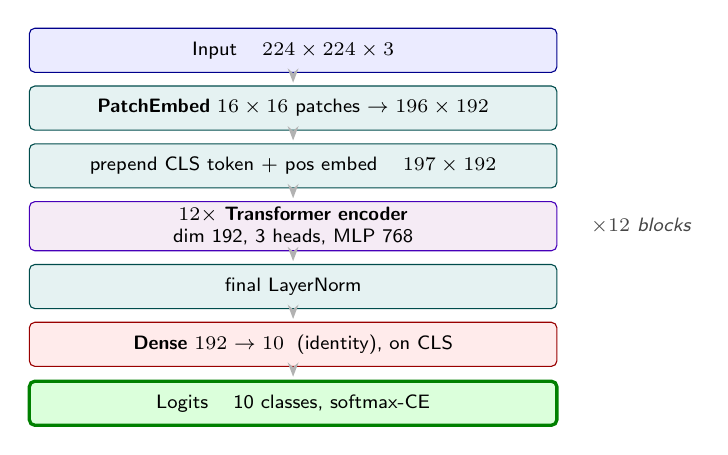
\begin{tikzpicture}[
  >={Stealth[length=1.8mm]},
  every node/.style={font=\sffamily\scriptsize},
  col/.style    = {align=center, rounded corners=2pt, inner sep=2pt, minimum height=0.56cm, minimum width=6.7cm},
  io/.style     = {col, draw=blue!55!black,   fill=blue!8},
  norm/.style   = {col, draw=teal!60!black,   fill=teal!10},
  blk/.style    = {col, draw=blue!45!violet,  fill=violet!8},
  head/.style   = {col, draw=red!60!black,    fill=red!8},
  logits/.style = {col, draw=green!50!black,  fill=green!14, very thick},
  arr/.style    = {->, thick, gray!60, shorten >=1pt, shorten <=1pt},
  stage/.style  = {font=\sffamily\scriptsize\itshape, gray!55!black, anchor=west},
]
  \node[io]                          (input){Input \;\; $224\times224\times3$};
  \node[norm, below=0.16cm of input] (pe)   {\textbf{PatchEmbed} $16\times16$ patches $\to 196\times192$};
  \node[norm, below=0.16cm of pe]    (cls)  {prepend CLS token $+$ pos embed \;\; $197\times192$};
  \node[blk, below=0.16cm of cls]    (enc)  {$12\times$ \textbf{Transformer encoder}\\dim 192, 3 heads, MLP 768};
  \node[norm, below=0.16cm of enc]   (ln)   {final LayerNorm};
  \node[head, below=0.16cm of ln]    (d)    {\textbf{Dense} $192\to10$ \;(identity), on CLS};
  \node[logits, below=0.16cm of d]   (out)  {Logits \;\; 10 classes, softmax-CE};
  \foreach \a/\b in {input/pe,pe/cls,cls/enc,enc/ln,ln/d,d/out}\draw[arr](\a)--(\b);
  \node[stage] at ($(enc.east)+(0.30,0)$){$\times 12$ blocks};
\end{tikzpicture}

\vspace{0.45cm}

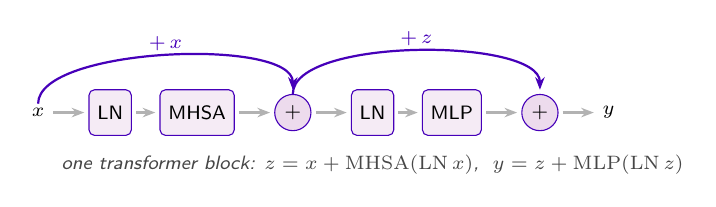
\begin{tikzpicture}[
  >={Stealth[length=1.6mm]},
  every node/.style={font=\sffamily\scriptsize},
  proc/.style={align=center, rounded corners=2pt, inner sep=3pt, minimum height=0.58cm, draw=blue!45!violet, fill=violet!8},
  op/.style  ={circle, draw=blue!45!violet, fill=violet!14, inner sep=0pt, minimum size=0.46cm},
  term/.style={font=\sffamily\scriptsize\itshape, inner sep=1.5pt},
  flow/.style={->, thick, gray!60, shorten >=1.5pt, shorten <=1.5pt},
  skip/.style={->, thick, blue!45!violet, shorten >=1.5pt},
]
  \node[term] (x){$x$};
  \node[proc, right=0.5cm of x]   (ln1){LN};
  \node[proc, right=0.35cm of ln1](mh){MHSA};
  \node[op,   right=0.5cm of mh]  (s1){$+$};
  \node[proc, right=0.5cm of s1]  (ln2){LN};
  \node[proc, right=0.35cm of ln2](ml){MLP};
  \node[op,   right=0.5cm of ml]  (s2){$+$};
  \node[term, right=0.5cm of s2]  (y){$y$};
  \foreach \a/\b in {x/ln1,ln1/mh,mh/s1,s1/ln2,ln2/ml,ml/s2,s2/y}\draw[flow](\a)--(\b);
  \draw[skip] (x.north) .. controls +(0,0.72) and +(0,0.72) .. (s1.north)
        node[midway, above, term, blue!45!violet]{$+\,x$};
  \draw[skip] (s1.north) .. controls +(0,0.72) and +(0,0.72) .. (s2.north)
        node[midway, above, term, blue!45!violet]{$+\,z$};
  \node[term, below=0.18cm of ln2, gray!55!black]{one transformer block: $z = x + \mathrm{MHSA}(\mathrm{LN}\,x)$, \ $y = z + \mathrm{MLP}(\mathrm{LN}\,z)$};
\end{tikzpicture}
\end{center}

\subsection*{The verified trainer}

\S\ref{sec:verified_trainer_pattern} is the pattern, and every chapter
since Chapter~\ref{chap:depthwise} has reused it. ViT drops the same one
of its four annotated points that ConvNeXt does. There is no
\texttt{bnChannels} here, because there is no BatchNorm.

\begin{verbatim}
import LeanMlir

-- 1. The network. `slug` names the committed render. No `bnChannels`:
--    LayerNorm keeps no running statistics, so nothing has to be
--    threaded from training into evaluation.
def vitVerified : VerifiedNetSpec where
  name     := "ViT-Tiny"
  slug     := "vit"
  inC      := 3
  imageH   := 224
  imageW   := 224
  nClasses := 10
  data     := .imagenette
  layers   := [
    .conv 3 192 16 16,          -- patch embed 16x16/s16, 224 -> 14x14 = 196
    .param #[192] 2,            -- CLS token
    .param #[197, 192] 2,       -- positional embedding, 196 + 1
    .transformerBlock 192 768,  -- 12 pre-norm blocks @ dim 192, MLP 768
    .transformerBlock 192 768,  .transformerBlock 192 768,
    .transformerBlock 192 768,  .transformerBlock 192 768,
    .transformerBlock 192 768,  .transformerBlock 192 768,
    .transformerBlock 192 768,  .transformerBlock 192 768,
    .transformerBlock 192 768,  .transformerBlock 192 768,
    .layerNorm 192,             -- final LayerNorm, per-channel
    .dense 192 10 ]             -- CLS-head 192 -> 10
  -- Stochastic depth, read only by the `*drop` variants. TWENTY-FOUR
  -- entries for TWELVE blocks: ViT drops a block's two residual
  -- branches independently, at one keep shared by the pair.
  dropKeeps := (Array.range 24).map (fun s =>
                 1.0 - 0.1 * (s / 2).toFloat / 11.0)

-- 2. The schedule. Note it is NOT the other four nets' schedule.
def vitAdamConfig : VerifiedConfig where
  epochs    := 80
  batchSize := 32

-- 3. The entry point: AdamW, cosine with a 5-epoch warmup,
--    baseLR 3e-4.
def main (argv : List String) : IO Unit :=
  vitVerified.toNet.trainAdamSched
    vitAdamConfig (argv.head?.getD "data")
    0.0003 0.9 0.999 5 "adam"
\end{verbatim}

\noindent The body is a patch embedding, twelve blocks and a head. The
patch embed is spelled \texttt{.conv 3 192 16 16}, a $16 \times 16$
kernel at stride 16, which chops the $224 \times 224 \times 3$ image
into $14 \times 14 = 196$ non-overlapping patches and projects each to
192 dimensions. That it is a convolution rather than a distinct
primitive is the point: a patch embedding \emph{is} a strided
convolution whose kernel equals its stride, so it reuses
Chapter~\ref{chap:cnn}'s proved backward and needs nothing new.

\textbf{The CLS token and the positional embedding are
\texttt{.param} entries.} They are learned weights that no layer
computes from an input, and the spec's job is the \emph{parameter
layout}, so it names them rather than folding them into a block. The
$197$ is $196$ patches plus the prepended CLS row.

\textbf{\texttt{.transformerBlock 192 768} is one block, not a stage.}
There is no repeat count, so twelve blocks are twelve entries, exactly
as ConvNeXt's eighteen were eighteen. Each carries the pre-norm
sandwich drawn in the inset above: LayerNorm, MHSA, residual,
LayerNorm, MLP, residual.

\textbf{The arm, and why sixteen tensors is the whole block.}

\begin{verbatim}
  | param dims kind    => #[(dims, kind)]              -- Ch. 9: CLS, pos-embed
  | transformerBlock d m =>                            -- Ch. 9
    #[(#[d],1),(#[d],2),                               -- LN1
      (#[d,d],0),(#[d],2), (#[d,d],0),(#[d],2),        -- Wq, Wk
      (#[d,d],0),(#[d],2), (#[d,d],0),(#[d],2),        -- Wv, Wo
      (#[d],1),(#[d],2),                               -- LN2
      (#[d,m],0),(#[m],2), (#[m,d],0),(#[d],2)]        -- MLP d->m->d
\end{verbatim}

\noindent \texttt{.param} is the escape hatch: a bare learned tensor with
no layer around it, which is how the CLS token and the positional
embedding get into the list at all. Everything else here is a dense
layer wearing a different name --- the four attention projections are
\texttt{[d,d]} matrices with biases, indistinguishable in the parameter
list from Chapter~\ref{chap:tensor}'s \texttt{.dense}. What makes them
attention is the \emph{graph}, not the shapes. Sixteen tensors a block,
twelve blocks, plus the patch embed, the two \texttt{.param}s, the final
LayerNorm and the head: 200.

\textbf{200 parameter tensors, 5,526,346 scalars.}
\texttt{vitVerified.toSpecs} is kernel-\texttt{\#guard}ed against
\texttt{ViTLayout.specs}, an independently audited hand-list, and the
ImageNet spec of \S\ref{sec:vit_imagenet} is pinned to this one at
everything but its head. At 1000 classes the count is 5,717,416. So the
listing above is not a description of the network that got trained, it
is the object the renderer consumed.

\textbf{Twenty-four keeps for twelve blocks, and the pairing is the
content.} ViT drops each block's attention branch and MLP branch
independently, but at the same keep probability, so sites $2i$ and
$2i+1$ share $\mathrm{keep}_i = 1 - 0.1i/11$. The driver needs one
entry per \emph{site} because it draws one Bernoulli stream per mask
input. Deriving twenty-four evenly spaced keeps from the site ordinal
instead would silently unpair them, and no structural check would
notice.

Note the learning rate is 0.0003 (a third of what the ConvNets
used) and warmup is 5 epochs (longer than the ConvNets' 3). ViTs
need gentler optimization schedules, because the attention
softmax is prone to collapse if gradients push logits too hard
early, and warmup keeps the first few epochs slow enough to avoid
that failure mode.

\subsection*{Results}
\label{sec:vit_results}

\S\ref{sec:vit_runit} has the run: 80 epochs at about 18 seconds each,
twenty-four minutes, $\mathbf{68.74\%}$ top-1 and $\mathbf{90.42\%}$
top-5. That completes the Part-1 column, and every row of it is now a
measurement on the verified XLA path at the same dataset, the same
eighty epochs, and one RTX 4060 Ti:

\begin{center}
\begin{tabular}{l r r r r r r}
\hline
Model            & Params  & MLIR       & Step time & Total    & Top-1 & Top-5 \\
\hline
ResNet-34        & 21.29M  & 729\,KB    & 220 ms    & 1.5 h    & 89.71\% & 98.27\% \\
MobileNet V2     &  2.24M  & 1{,}047\,KB &  90 ms   & 35 min   & 89.25\% & \textbf{98.68\%} \\
EfficientNet-B0  &  4.02M  & 1{,}316\,KB & 103 ms   & 41 min   & \textbf{89.96\%} & 98.45\% \\
ConvNeXt-T       & 27.83M  & 985\,KB    & 196 ms    & 1.3 h    & 85.07\% & 97.30\% \\
ViT-Tiny         &  5.53M  & 1{,}282\,KB & \textbf{61 ms} & \textbf{24 min} & 68.74\% & 90.42\% \\
\hline
\end{tabular}
\end{center}

\noindent Step time is the epoch wall-clock divided by 295 batches, so
it includes each epoch's validation pass. MLIR sizes are the committed
\texttt{<slug>\_adam\_train\_step.mlir} in 1000-byte units.

ViT-Tiny is the fastest per step by a factor of $1.5$ over the next
network and the lowest-accuracy by more than sixteen points. That gap
is the data-hunger effect: 9,469 training images is tiny for a
transformer. The ViT paper reached ImageNet-competitive accuracy only
when trained on ImageNet-21K (14M images) or JFT-300M (300M images). At
Imagenette scale the ConvNets' inductive bias, locality and translation
equivariance, actively helps, and the ViT has to learn those properties
from data it doesn't have. \S\ref{sec:vit_imagenet} is the control:
the same architecture on 1.28M images reaches $70.28\%$ over a
\emph{thousand} classes, which is the regime the design was for.

\medskip\noindent\textbf{It reproduces exactly.} Chapter~\ref{chap:cnn}'s
width sweep is where this book first had to take run-to-run spread
seriously, so this number was measured three times before being printed,
and all three passes came back \emph{bit-identical} on three different
cards: the same $68.738854\%$ and $90.420382\%$ at epoch 80, and the same
160 epoch lines the whole way down. That makes ViT the first network since
the dense-only graphs of Chapter~\ref{chap:mlp} to reproduce exactly, and
for the same reason. XLA selects convolution algorithms per process, which
is what moves the convnet chapters' numbers by a point or two between
runs. This graph holds 435 \texttt{dot\_general}s and \emph{two}
convolutions, so there is almost nothing for that selection to vary.

\section{MLIR: Attention}

\noindent\textbf{What is already proven.} Scaled dot-product
attention is $\mathrm{sdpa}(Q,K,V) = \mathrm{softmax}(QK^{\!\top}/\sqrt{d})\,V$.
Its reverse-mode derivative produces three gradients ($dQ$, $dK$, $dV$),
each proven separately (\S\S~\ref{thm:sdpa_back_Q_correct}--%
\ref{thm:sdpa_back_V_correct}, \texttt{sdpa\_back\_Q/K/V}), all built on the
softmax backward, which couples every position to every other
(\S~\ref{thm:softmax_has_vjp}). Because $Q$, $K$, and $V$ are three linear
projections of the \emph{same} input $a$, the input gradient is a three-way
fan-in, $da = dQ\,W_q^{\!\top} + dK\,W_k^{\!\top} + dV\,W_v^{\!\top}$.
\texttt{sdpa\_has\_vjp\_mat3} bundles the three, and
\texttt{transformerAttnSublayer\_has\_vjp\_mat} composes the whole sublayer
(LayerNorm, the QKV projections, attention, the output projection, the
residual) through \texttt{vjp\_comp\_at}.

\medskip\noindent\textbf{The gap and how we close it.} The softmax backward
is non-elementwise and the three projections are coupled. The emitted graph
denotes \texttt{transformerAttnSublayer\_has\_vjp\_mat}'s backward. Here is
the three-way fan-in at the input (two tokens, model dimension four, single
head, with the SDPA backward that produces $dQ,dK,dV$ elided to its comment):

\begin{verbatim}
// dQ,dK,dV = SDPA.back(dOut . Wo^T)  (softmax-weighted attention grads)
%daQ = stablehlo.dot_general %dQ, %Wq, contracting_dims = [1] x [1]
         : (tensor<2x4xf32>, tensor<4x4xf32>) -> tensor<2x4xf32>
%daK = stablehlo.dot_general %dK, %Wk, contracting_dims = [1] x [1]
         : (tensor<2x4xf32>, tensor<4x4xf32>) -> tensor<2x4xf32>
%daV = stablehlo.dot_general %dV, %Wv, contracting_dims = [1] x [1]
         : (tensor<2x4xf32>, tensor<4x4xf32>) -> tensor<2x4xf32>
%daQK = stablehlo.add %daQ, %daK : tensor<2x4xf32>
%da = stablehlo.add %daQK, %daV : tensor<2x4xf32>
// %dxa = LN.back(%da);  %dx = %dOut + %dxa  (residual skip)
\end{verbatim}

\noindent Read it against the fan-in: each \texttt{dot\_general} carries one
of the attention gradients back through its projection ($dQ$ through $W_q$,
and so on, contracting the model axis), and the two \texttt{add}s sum the
three. This is the residual fan-in of Chapter~\ref{chap:residual} with three
branches instead of one, because attention reads the input thrice, so the
gradient returns thrice and adds. The softmax-weighted $dQ,dK,dV$ that feed the
\texttt{dot\_general}s come from the proven \texttt{sdpa\_back\_Q/K/V}, and
the surrounding LayerNorm and output projection chain through their bridges.

\medskip\noindent One honesty note: the hard part of attention is in that
first comment. This listing is the \emph{projection} fan-in (three linear
adjoints and two adds), while the softmax backward that couples every token
to every other (\texttt{softmax\_has\_vjp}, \S~\ref{sec:attention_proofs}) is
what \texttt{// SDPA.back} stands in for. We show the fan-in because it is the
new \emph{structural} move. The coupled core is carried by the proofs of
\S~\ref{sec:attention_proofs}.

\medskip\noindent With attention pinned, the verified-codegen thread covers
every operator in the modern vision stack, and that means dense, convolution,
BatchNorm, residual, depthwise, squeeze-excite, layer scale and attention.
Each is emitted as the rendering of a machine-checked derivative, from the
same three pieces: denoted IR, bridge theorem, printer.

\medskip\noindent\textbf{Caveats.}
\begin{itemize}
  \item \textbf{The attention bridge is unconditional.} Softmax and the
    linear projections are smooth everywhere, with no smooth-point clause.
  \item \textbf{Representative scale} (two tokens, $d = 4$, one head).
\end{itemize}

\section{ImageNet recipe}

\imagenettimmnote
\label{sec:vit_imagenet}

\imagenetphasenote

The Imagenette ViT-Tiny above trained on $\sim$9.5K images. The
full 1000-class run is the same architecture with a 1000-class head,
the \texttt{.imagenet} dataset, and the DeiT-flavored training recipe,
so it is still patch16, embed 192, 12 transformer blocks and 3 heads,
at 5{,}717{,}416 parameters. This is the \textbf{phase-2 reference}
implementation, \texttt{jax/MainVitImagenet.lean}, quoted as it stands
today:

\begin{verbatim}
-- 1. Same ViT-Tiny backbone, 1000-class head.
def vitTinyImagenet : NetSpec where
  name   := "ViT-Tiny (ImageNet, bf16)"
  imageH := 224
  imageW := 224
  layers := [
    .patchEmbed 3 192 16 196,            -- (224/16)^2 = 196 patches
    .transformerEncoder 192 3 768 12,    -- 12 blocks, 3 heads, MLP 768
    .dense 192 1000 .identity            -- 1000-class head
  ]

-- 2. Full DeiT-Ti recipe: AdamW, cosine, the aug suite, stochastic depth, EMA.
def vitTinyImagenetConfig : TrainConfig where
  learningRate      := 5e-4          -- proper DeiT batch-512 LR
  batchSize         := 512
  epochs            := 300           -- full DeiT-Ti schedule
  useAdam           := true          -- AdamW (decoupled weight decay)
  weightDecay       := 0.05
  wdExcludeNormBias := true          -- no_weight_decay: skip norm/bias/pos-embed/CLS
  cosineDecay       := true
  warmupEpochs      := 5
  labelSmoothing    := 0.1
  gradClipNorm      := 1.0           -- the unlock for the 5e-4 LR (see below)
  useMixup          := true          -- Mixup alpha 0.8
  useCutmix         := true          -- CutMix alpha 1.0 (alternates with Mixup)
  useRandAugment    := true          -- rand-m9-mstd0.5-inc1 (color + geometric)
  randomErasing     := true          -- Random-Erase p 0.25
  dropPath          := 0.1           -- stochastic depth (linear 0 -> 0.1)
  useEMA            := true          -- model EMA decay 0.99996 (eval on shadow)
  bf16              := true          -- bf16 matmul compute
  valEveryEpochs    := 5             -- ImageNet val is data-loading-bound
  repeatedAug       := 3             -- DeiT Repeated Augmentation (see below)

-- 3. The phase-2 reference driver. The verified path's entry point is
--    trainAdamSched, in the phase-4 subsection at the end of this chapter.
def main (args : List String) : IO Unit :=
  vitTinyImagenet.train vitTinyImagenetConfig
    (args.head?.getD "data/imagenet") .imagenet
\end{verbatim}

As with the ResNet-34 ImageNet run (Ch~\ref{chap:residual}), that
driver wires \texttt{.imagenet} through tfds streaming. The verified
path reads the same 1.28M-image stream through a generated shim of
its own, and it has a trainer built and running at this scale.
\S\ref{sec:vit_phase4} is that side of it. The numbers in this
section are the reference implementation's.

\textbf{The stability knob.} ViT-Tiny is where the recipe stops
being optional. At the proper DeiT learning rate (peak $5\times
10^{-4}$ for batch 512) the model \emph{collapses to chance} the
moment warmup ramps the LR past ${\sim}1.6\times 10^{-4}$, with train
loss pinned at $\ln(1000)\approx 6.9$ and never recovering. This is the
well-known no-grad-clip transformer instability, sharpened here by
the 1000-class softmax and bf16 gradient noise. The fix is one
field: \texttt{gradClipNorm := 1.0}, global-norm gradient clipping,
the DeiT default. With it, the very LR that collapsed without it
trains cleanly through warmup and on to convergence.

\textbf{bf16 and the run.} ViT is matmul-bound, because the patch
embed, the attention QKV/scores/output, the MLP and the head are all
dense matrix multiplies, with no convolution to speak of. So unlike the
ResNet case, the relevant precision flag is \texttt{bf16} alone
(matmul compute in bfloat16, fp32 master weights, fp32
LayerNorm/softmax/GELU), and there is no \texttt{bf16Conv} to set.
bf16 matmul runs through the same NVIDIA tensor cores. Measured on
the same four RTX 4060 Ti (CUDA) at batch 512, bf16 is
$\mathbf{1.48\times}$ faster per step than fp32 ($176$ vs $260$\,ms
steady-state), a smaller multiple than the convnet's
$1.6\times$, since ViT-Tiny's matmuls are narrow (embed $192$) and
spend proportionally more time in the fp32 LayerNorm/softmax that
bf16 leaves untouched. On the ROCm box the effect is
\emph{larger}, not smaller: RDNA3's matmul units (WMMA) give bf16 a
$\mathbf{2.75\times}$ compute speedup on the full ViT-Tiny step
($428 \to 156$\,ms for forward + backward + AdamW at batch
$256$/GPU), diluting to ${\sim}2\times$ end-to-end once the fp32
LayerNorm/softmax and the tfds pipeline fold back in. The convnets
see no such lift on gfx1100, because MIOpen's bf16 convolution is no
faster than fp32 there, but ViT is all matmul, so the win is
real. The runs:

\begin{center}
\begin{tabular}{l l r r r r r}
\hline
GPU & Precision & Per epoch & Epochs & Wall-clock & Val top-1 & Val top-5 \\
\hline
4$\times$ 4060 Ti (CUDA) & bf16 & $\sim$7.6 min & 300 & $\sim$41 hr & --- & --- \\
2$\times$ 7900 XTX (ROCm) & bf16 & $\sim$10 min & 300 & $\sim$50 hr & $\mathbf{70.28\%}$ & $\mathbf{90.05\%}$ \\
\hline
\end{tabular}
\end{center}

\noindent The CUDA row is the measured per-epoch rate carried out to the
full schedule rather than a completed run, which is why it reports no
accuracy. The result below is the ROCm one.

The full 300-epoch DeiT-Ti recipe reached $\mathbf{70.28\%}$ top-1 /
$\mathbf{90.05\%}$ top-5 on the full 50{,}000-image validation split.
That lands within ${\sim}2$ points of the ${\sim}72\%$ ViT-Tiny is
capable of. The candidates for the remaining gap are the one recipe knob
that run did not have (repeated augmentation) plus two minor deviations
(strict Mixup/CutMix alternation instead of a random switch, and
Random-Erase to zero rather than to noise) --- candidates rather than an
accounting, since this section's numbers predate the resampler change. The headline is a \emph{300-epoch} DeiT
result with the full distillation-free recipe, and the point here is
the pipeline (proven attention backward $\to$ DeiT recipe $\to$ stable
bf16 training to a sensible ImageNet number), not a SOTA chase. The
validation curve shows the familiar shape, a fast climb through warmup,
a long middle, and a final lift as the cosine schedule anneals to zero:

\begin{center}
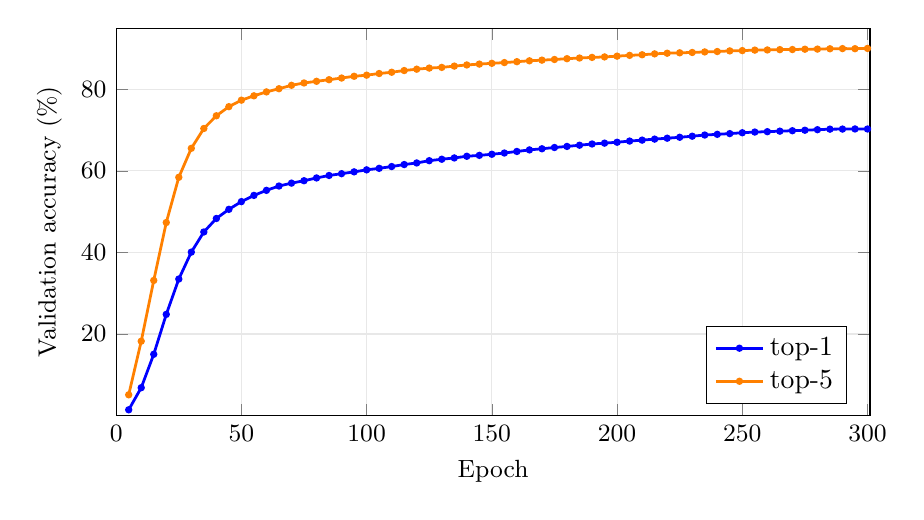
\begin{tikzpicture}
\begin{axis}[
    width=0.92\linewidth, height=6.5cm,
    xlabel={Epoch}, ylabel={Validation accuracy (\%)},
    xmin=0, xmax=301, ymin=0, ymax=95,
    xtick={0,50,100,150,200,250,300},
    ytick={20,40,60,80},
    legend pos=south east,
    legend cell align={left},
    grid=major, grid style={gray!18},
    tick label style={font=\small},
    label style={font=\small},
    every axis plot/.append style={line width=1pt, mark size=0.8pt},
]
\addplot[blue, mark=*, mark options={fill=blue}] coordinates {
(5,1.40) (10,6.82) (15,15.02) (20,24.81) (25,33.47) (30,40.08) (35,45.02) (40,48.33) (45,50.57) (50,52.47) (55,53.99) (60,55.23) (65,56.29) (70,57.00) (75,57.59) (80,58.27) (85,58.88) (90,59.32) (95,59.77) (100,60.26) (105,60.63) (110,61.07) (115,61.56) (120,61.95) (125,62.51) (130,62.86) (135,63.18) (140,63.59) (145,63.81) (150,64.08) (155,64.39) (160,64.77) (165,65.15) (170,65.43) (175,65.74) (180,66.00) (185,66.30) (190,66.60) (195,66.81) (200,67.03) (205,67.32) (210,67.55) (215,67.80) (220,68.02) (225,68.25) (230,68.51) (235,68.80) (240,68.97) (245,69.15) (250,69.36) (255,69.53) (260,69.62) (265,69.75) (270,69.86) (275,69.98) (280,70.11) (285,70.24) (290,70.26) (295,70.29) (300,70.28)
};
\addlegendentry{top-1}
\addplot[orange, mark=*, mark options={fill=orange}] coordinates {
(5,5.08) (10,18.23) (15,33.13) (20,47.34) (25,58.43) (30,65.54) (35,70.40) (40,73.52) (45,75.76) (50,77.35) (55,78.42) (60,79.38) (65,80.16) (70,81.00) (75,81.57) (80,81.98) (85,82.37) (90,82.78) (95,83.21) (100,83.48) (105,83.89) (110,84.20) (115,84.62) (120,84.95) (125,85.22) (130,85.39) (135,85.71) (140,85.99) (145,86.20) (150,86.39) (155,86.57) (160,86.79) (165,87.01) (170,87.17) (175,87.33) (180,87.53) (185,87.69) (190,87.84) (195,87.96) (200,88.15) (205,88.34) (210,88.49) (215,88.71) (220,88.87) (225,88.97) (230,89.05) (235,89.19) (240,89.28) (245,89.44) (250,89.51) (255,89.63) (260,89.67) (265,89.75) (270,89.77) (275,89.85) (280,89.88) (285,89.96) (290,90.00) (295,89.98) (300,90.05)
};
\addlegendentry{top-5}
\end{axis}
\end{tikzpicture}
\end{center}

\noindent ViT-Tiny / ImageNet-1k validation accuracy per epoch (bf16,
2$\times$ RX 7900 XTX, ROCm, sampled every 5 epochs across the 300-epoch
run).

\textbf{Distance to the paper.} DeiT-Ti reaches $72.2\%$ without
distillation. Our $70.28\%$ is ${\sim}2$ points short, and the
accounting is mundane. The largest single item is \emph{repeated
augmentation}, where DeiT samples each image in a batch three times
under different augmentations, which disproportionately helps the
data-hungry tiny models. The run that produced $70.28\%$ did not have
it. The recipe does now, as the \texttt{repeatedAug := 3} in the
listing above, and it landed after that run had already finished. So
repeated augmentation is the obvious next lever, and the accurate
statement about it is that it is untested here rather than missing.
The rest is augmentation-fidelity drift, since RandomResizedCrop and
Random-Erasing are a from-scratch \texttt{tf.data} reimplementation
rather than timm's exact code (our RandAugment now matches timm's
\texttt{rand-m9-mstd0.5-inc1} op-set literally), plus a few small
knobs (batch $512$ vs.\ $1024$, the gradient clipping we add for
stability, Random-Erase to zero rather than to noise). None of it is
a bug: the loss curve is textbook DeiT. The further $+2.3$ points to
DeiT-Ti's $74.5\%$ headline are a different thing entirely, the
\emph{distillation} variant (a second ``distillation token'' trained
against a strong CNN teacher), which we do not implement.

\textbf{[TODO: re-run on the current config.]}
\texttt{vit-tiny-imagenet}, \textbf{300 epochs}, a re-run of the
$70.28\%$ above. \emph{Changed since that number:} RandAugment is now
timm-literal (\texttt{rand-m9-mstd0.5-inc1}: SolarizeAdd$+$Invert
op-set, per-op apply prob $0.5$, bilinear geometric interpolation,
relative translate), and repeated augmentation is now in the recipe at
$3\times$. Re-running with both is the path to close the $\sim$2 points
to DeiT-Ti's $72.2\%$.

\subsection*{Phase 4: the verified trainer}
\label{sec:vit_phase4}

Everything above this point is the phase-2 Lean$\to$JAX trainer. The
phase-4 peer, which trains the same network through the proof-rendered
StableHLO that \S\ref{sec:vit_runit} ran at Imagenette scale, exists and
builds. It is \texttt{apps/imagenette/MainViTImagenet.lean}, built as
\texttt{lake build vit-imagenet-verified}:

\begin{verbatim}
-- Identical backbone, 1000 classes instead of 10.
def vitImagenetVerified : VerifiedNetSpec where
  name       := "ViT-Tiny (ImageNet-1k)"
  slug       := "vitin"
  nClasses   := 1000
  data       := .imagenet
  shimScript := "generated_vit_tiny_imagenet_shim.py"
  layers     := [ ... the Imagenette stack, 1000-class head ... ]

-- 300 epochs, because that is the schedule the phase-2 number
-- above was measured on. Batch is 128 PER DEVICE, so four
-- replicas give the reference's global 512 exactly.
def vitImagenetConfig : VerifiedConfig where
  epochs    := 300
  batchSize := 128
\end{verbatim}

\noindent The head is the only parameter shape that moves, from
$192 \times 10$ to $192 \times 1000$, which takes the count from
5,526,346 to \textbf{5,717,416}. The same three kernel \texttt{\#guard}s
that hold ConvNeXt's two specs together hold these: equal
\texttt{toSpecs.size}, equal \texttt{toSpecs.pop.pop}, and a
\texttt{back!} of \texttt{(\#[1000], 2)}.

\medskip\noindent\textbf{The collectives are gated one way here, and it
is worth saying which.} \texttt{tests/TestViTDpCheck.lean} pins the
data-parallel step against its single-device peer by handing both
replicas the \emph{same} rows, where the all-reduce mean is an
identity. ViT has no BatchNorm, so that identity is exact rather than
approximate. But a gate built on duplicated rows is structurally blind
to a shard-offset bug, and the check that closes that hole works by
giving the replicas genuinely different data. That one now covers the
Imagenette \texttt{vit} spec, and it does not yet cover \texttt{vitin}.
Two gates that sound alike are not one property, and this chapter has
one and a half of them rather than ConvNeXt's two.

\medskip\noindent\textbf{The regularizer knobs are render variants, and
the same combination is missing here as there.} Weight-decay exclusion,
grad clipping and stochastic depth are spelled \texttt{wx},
\texttt{clip} and \texttt{drop}, and
\texttt{vitin\_adamdp128x4wxclipdrop} carries all three at once on top
of AdamW and the four-way all-reduce. EMA is a variant too
(\texttt{vitin\_emadp128x4}), but no committed artifact combines it with
the other three. Mixup, CutMix and repeated augmentation never enter the
graph at all, because they are data-side and ride the shim.

\medskip\noindent\textbf{What it has not done is run.} No phase-4
ImageNet result exists for this network, which is why every accuracy
above comes from phase 2. What is measured is the throughput, and the
schedule follows from it:

\begin{center}
\begin{tabular}{l r r r r}
\hline
Box & ms/step & min/epoch & 300 epochs & Val top-1 \\
\hline
4$\times$ 4060 Ti (CUDA)  & 163 &  6.8 & $\sim$37.1 h (1.5 d) & TBD \\
4$\times$ 3060 (CUDA)     & 159 &  6.6 & $\sim$36.3 h (1.5 d) & TBD \\
\hline
\end{tabular}
\end{center}

\noindent At global batch 512 that is 2,502 steps per epoch, which is
the reference's own figure. \textbf{Nothing confounds this
comparison.} The batch does \emph{not} differ, unlike Chapter~\ref{chap:layernorm}'s
phase-4 row, where the render's smaller per-device batch confounded it a
second way; and precision no longer differs either, since the verified
renders gained a bf16 arm and the row above is measured on it. What that
leaves is the one place in Part 1 where the verified row is the
\emph{faster} of the two, at 6.8 minutes per epoch against phase 2's 7.6.
It is also the fastest phase-4 epoch in Part 1, ahead of MobileNetV2's
10.8 and ResNet-34's 18.6, though the 300-epoch schedule still makes it a longer
run in total than Chapter~\ref{chap:residual}'s ninety.

\noindent\textbf{[TODO: run \texttt{vit-imagenet-verified}.]}

\subsection*{What Part 1 has established}

Every layer primitive shipped in Part 1's trainers (MLP,
CNN, ResNet, MobileNet, EfficientNet, ConvNeXt, ViT) has a
machine-checked backward pass. The same \texttt{VerifiedNetSpec} /
\texttt{VerifiedConfig} / \texttt{trainAdamSched} pipeline trains all
of them with at most config-level changes. The MLIR each emits is
between 7\,KB (MLP) and 1{,}316\,KB (EfficientNet-B0), and the
lowerer compiles all of them the same way.

The bestiary in Part 2 then shows that \emph{every other
architecture you've seen in modern deep learning} composes from the
same small set of primitives plus a handful of
architecture-specific bundled layers. That list runs UNet, YOLO, DETR,
Mask R-CNN, DCGAN, CycleGAN, Pix2Pix, DDPM, Stable Diffusion, VAE,
AlphaGo, AlphaZero, MuZero, Mamba, BERT, GPT, Whisper, CLIP, LLaVA,
SAM, SegFormer, DeepLab v3+, Nyström-former, QANet and Evoformer. Three rules (chain, additive
fan-in, multiplicative fan-in). Five Jacobian tricks (diagonal,
sparse Toeplitz, binary selection, rank-1 correction, outer
product).

That's the whole framework. Part~2's bestiary takes the same set
of primitives and tours how they compose into every well-known
modern architecture, a survey of the field expressed in the
proven kit, with a small library of bundled idioms for the patterns
that recur.

\section{Side quest: ViT-S and ViT-B}
\label{sec:vit_sb}

ViT scales on one axis where ConvNeXt scaled on two. Tiny, Small and Base are
the same twelve blocks at a wider model dimension: $D = 192/3$ heads,
$384/6$, $768/12$, with the MLP at $4D$ throughout. Depth never moves.

\begin{center}
\begin{tabular}{@{}l c c r r@{}}
\hline
model & $D$ / heads & params & per-dev bs & 4 cards: fp32 $\to$ bf16 \\
\hline
ViT-Ti & $192$ / 3  & $5.7$\,M         & $128$ & $171.6 \to 96.4$\,ms \;($1.78\times$) \\
ViT-S  & $384$ / 6  & $22{,}050{,}664$ & $128$ & $464.0 \to 245.5$\,ms \;($\mathbf{1.89\times}$) \\
ViT-B  & $768$ / 12 & $86{,}567{,}656$ & $32$  & $383.8 \to 273.7$\,ms \;($1.40\times$) \\
\hline
\end{tabular}
\end{center}

\noindent Counts \texttt{\#guard} against DeiT-S's $22.05$\,M and DeiT-B's
$86.57$\,M. These are the graph's times, all-reduce in and no trainer around
them, at four replicas because S and B have no single-device render at all.
\texttt{vitbin} runs at global $128$: the one place in Part~I where a model's
size rather than its recipe dictates how it must be run.

\medskip\noindent \textbf{ViT-S's $1.89\times$ is the largest bf16 payoff in the
book}, ahead of ResNet-50's $1.66\times$ measured the same way, and the spread
across one architecture is the interesting part. Tiny is narrow enough that its matmuls underuse the
tensor cores even in bf16; S's $D = 384$ suits them; B pays a $346$\,MB
\emph{fp32} all-reduce every step at batch $32$, a fixed cost in both arms.
The one op where bf16 \emph{loses} here --- the stem weight gradient, at
$0.19\times$ for want of a bf16 kernel at a $209\times209$ window --- is kept out
of the emit at every size, which is why all three ratios are above one.

\medskip\noindent Where \S\ref{sec:convnext_sb} found a split between free and
costly, ViT is uniformly costly: every variant moves $D$, so every variant moves
dimension literals. The batched renderer carries all three;
\texttt{ViTRender.lean}, the per-example peer, is still pinned at Tiny by roughly
$154$ of them, which is why there is no ViT-S or ViT-B Imagenette demo.

\medskip\noindent \textbf{A full schedule.} Trainer steps, all three measured
on real ImageNet over $40$ steps at four cards, $300$ epochs, totals including
$37.5$\,s per epoch of evaluation and checkpointing:

\begin{center}
\begin{tabular}{@{}l r r r r@{}}
\hline
verified, 4 cards & global & steps/epoch & ms/step & 300 epochs \\
\hline
ViT-Ti & $512$ & $2{,}502$  & $237 \to 168$ & $53 \to 38$\,h \;($2.2 \to 1.6$\,d) \\
ViT-S  & $512$ & $2{,}502$  & $528 \to 325$ & $113 \to 71$\,h \;($4.7 \to 3.0$\,d) \\
ViT-B  & $128$ & $10{,}009$ & $423 \to 317$ & $356 \to 268$\,h \;($14.8 \to 11.1$\,d) \\
\hline
\end{tabular}
\end{center}

\noindent Tiny is the control: it reads $237 \to 168$ here against a previously
committed $232 \to 163$, so the session runs about $2$--$3\%$ slow and the other
two rows can be read on the same basis.

\medskip\noindent \textbf{ViT-B's row exists because these were measured rather
than modelled, and the first attempt to model them was wrong.} Scaling Tiny's
trainer step by the ratio it bears to its own graph time overestimates ViT-S by
$19\%$. The reason is worth keeping: because the device figures above are
already four-replica, the all-reduce is inside them, so the only thing a trainer
adds is the data feed --- and that is roughly $65$\,ms at $128$ images per
device for \emph{both} Tiny and S, an additive constant rather than a
multiplier. \S\ref{sec:convnext_sb}'s figures are single-device, so there the
trainer must also absorb an all-reduce that grows with the parameter count, and
a multiplier is the right shape. Same box, same two quantities, two different
laws --- which is why the numbers above are probes and not arithmetic.

\medskip\noindent \textbf{Status: rendered, not trained}, the same as ConvNeXt's
pair --- \texttt{vit-s-\allowbreak imagenet-\allowbreak verified} and
\texttt{vit-b-\allowbreak imagenet-\allowbreak verified} emit, tie and step. The
only accuracy calibration that exists is this repo's ViT-Ti at $70.28\%$ against
DeiT-Ti's $72.2\%$, a $1.9$-point recipe gap (\S\ref{sec:vit_imagenet}). DeiT
quotes $79.8\%$ for S and $81.8\%$ for B; every item missing from that $1.9$ is
\emph{regularization} and S has four times Tiny's capacity, so the gap plausibly
widens rather than holds.

\medskip\noindent The phase-2 peers, same box at global $512$, cost $25.8$,
$60.4$ and $146.1$ hours over $300$ epochs compute-only. \textbf{B is the only
one that is not a single forward}: global $512$ in one shot peaks at $11.41$ of
the allocator's $11.68$\,GiB and dies, so it runs as $4\times128$ accumulation.

\chapter{Bestiary of Architectures}
\label{chap:bestiary}

% The bestiary is a catalogue, not a narrative: its subsection headings are
% the entries a reader looks up by name, so this chapter alone shows them in
% the TOC. Restored to depth 1 before the appendices below.
\addtocontents{toc}{\protect\setcounter{tocdepth}{2}}

Part 1 introduced a small set of \texttt{NetSpec} primitives across
chapters 1--9 and proved each one's backward pass:

\begin{itemize}
  \item Atomic ops: \texttt{.dense}, \texttt{.flatten},
    \texttt{.conv2d}, \texttt{.maxPool}, \texttt{.convBn},
    \texttt{.globalAvgPool}, plus the \texttt{Activation} enum
    (Ch 2--5).
  \item \texttt{.residualBlock} (Ch 5, ResNet-34).
  \item \texttt{.invertedResidual} (Ch 6, MobileNet V2).
  \item \texttt{.mbConv} with optional Squeeze-and-Excitation
    (Ch 7, EfficientNet-B0).
  \item \texttt{.convNextStage} + \texttt{.convNextDownsample}
    (Ch 8, ConvNeXt-T).
  \item \texttt{.patchEmbed} + \texttt{.transformerEncoder}
    (Ch 9, ViT-Tiny).
\end{itemize}

Call this the \emph{primary-sequence toolbox} --- everything a
reader has internalized after finishing Part 1. The \textbf{bestiary}
is Part 2: a catalogue of famous architectures expressed as pure
\texttt{NetSpec} values, no training runs, no VJP commitments, just
``here's what this architecture looks like in $\sim$15 lines of Lean.''

\paragraph*{What ``\(N\) new primitives'' means.}
Every bestiary entry leads with how many new \texttt{Layer}
constructors it asks the reader to absorb \emph{on top of the
primary-sequence toolbox}.

\begin{itemize}
  \item \emph{Zero new primitives} means the architecture composes
    entirely from things you already know --- VGG (just $3\times 3$
    conv stacks), AlphaZero (\texttt{convBn} + \texttt{residualBlock}),
    Highway Networks (two parallel \texttt{dense} paths plus a blend
    that's just product rule + additive fan-in from Ch 1). The
    architecture is conceptually a free read.
  \item \emph{One new primitive} means one bundled architectural
    idiom that wasn't in Part 1 --- \texttt{.bottleneckBlock} for
    deeper ResNets, \texttt{.fireModule} for SqueezeNet,
    \texttt{.mambaBlock} for Mamba, etc. The primitive is bundled
    at the right abstraction level (a whole Mamba block, a stage of
    Swin attention) so reading it is one chunk, not twenty
    sub-ops.
  \item \emph{Two or three new primitives} are reserved for
    architectures that genuinely combine multiple novel idioms ---
    DETR (\texttt{.transformerDecoder} + \texttt{.detrHeads}),
    DenseNet (\texttt{.denseBlock} + \texttt{.transitionLayer}),
    Stable Diffusion (\texttt{.unetDown} + \texttt{.unetUp} +
    \texttt{.transformerDecoder}). At most three; if you'd need
    more, the architecture probably warranted its own chapter.
\end{itemize}

This count is calibrated to the \emph{reader} (what's new vs.\ what
they've seen), not to the codebase (where some bestiary primitives
were drafted earlier and already sit in \texttt{Types.lean}).
Formalizing every sub-op of every modern architecture would be an
asymptote we don't approach.

\begin{center}
\resizebox{\textwidth}{!}{%
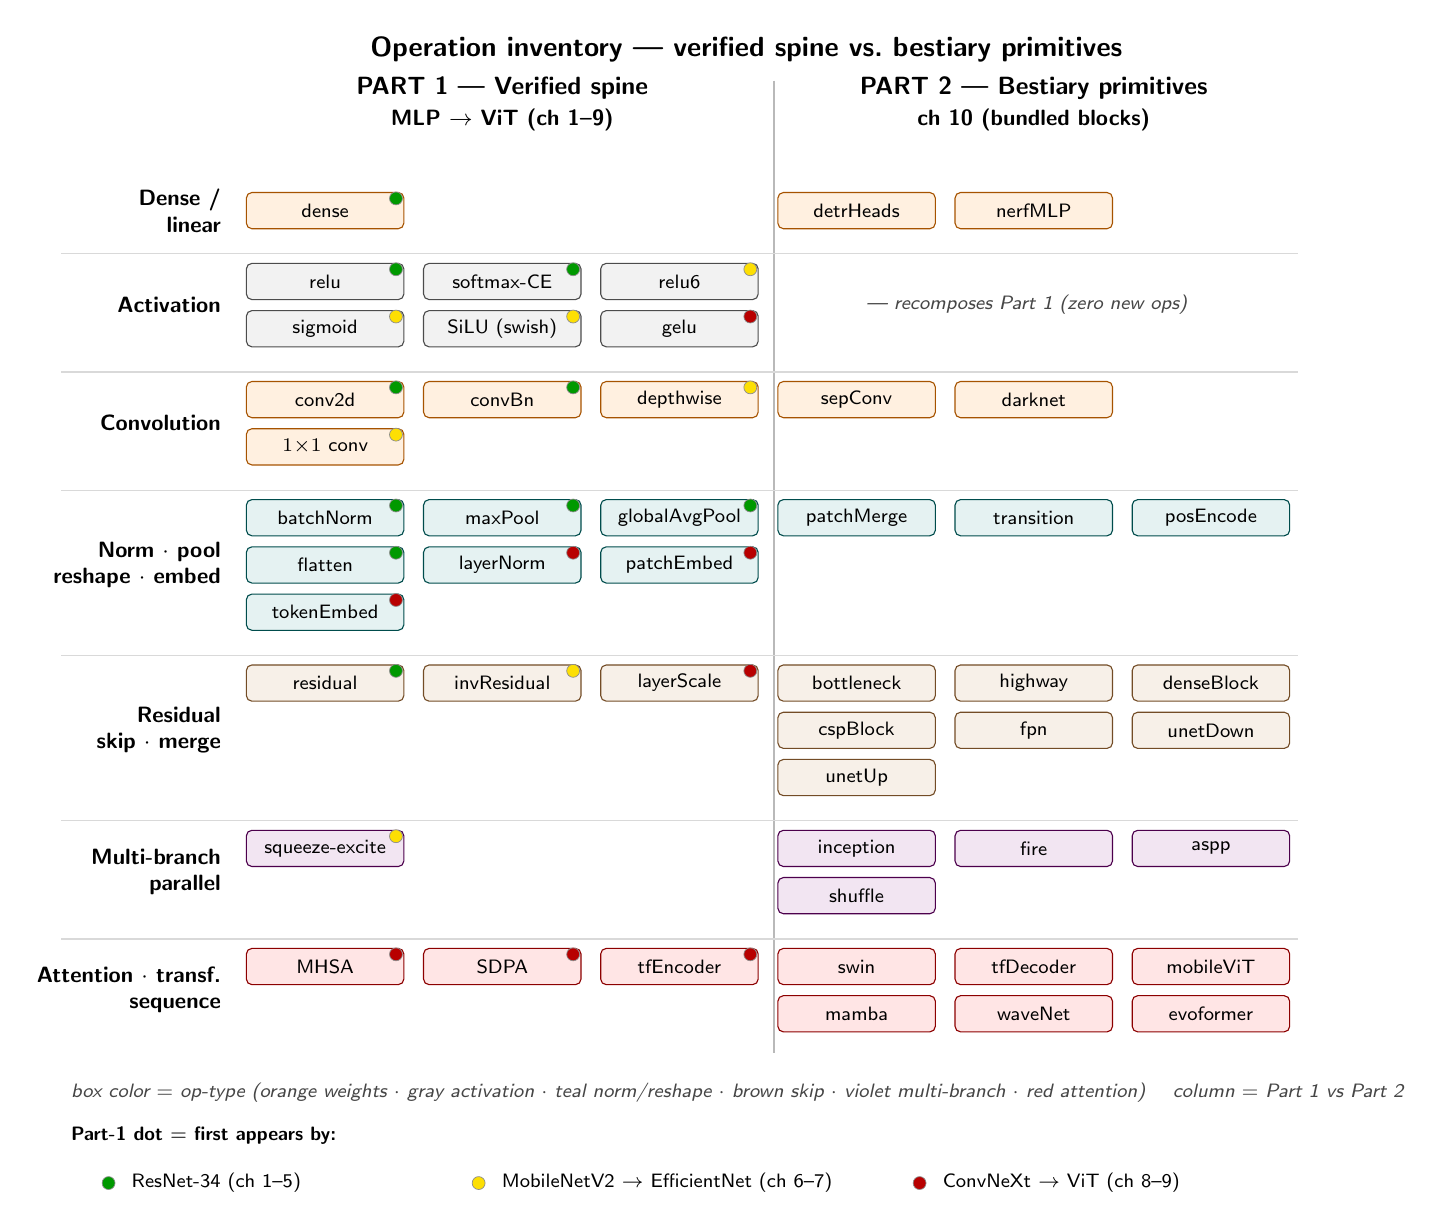
\begin{tikzpicture}[
  font=\sffamily,
  chip/.style = {draw, rounded corners=2pt, align=center, minimum height=0.46cm, minimum width=2.0cm, font=\sffamily\scriptsize, inner sep=1pt},
  cOr/.style  = {chip, draw=orange!65!black, fill=orange!12},
  cGy/.style  = {chip, draw=gray!60!black,   fill=gray!10},
  cTe/.style  = {chip, draw=teal!60!black,   fill=teal!10},
  cBr/.style  = {chip, draw=brown!60!black,  fill=brown!12},
  cVi/.style  = {chip, draw=violet!60!black, fill=violet!10},
  cRd/.style  = {chip, draw=red!55!black,    fill=red!10},
  catlbl/.style = {font=\sffamily\bfseries\footnotesize, align=right, anchor=east},
  hdr/.style  = {font=\sffamily\bfseries\small, align=center},
  emptylbl/.style = {font=\sffamily\scriptsize\itshape, gray!55!black, anchor=west},
  band/.style = {gray!30, line width=0.4pt},
]
% wrapping row of chips (3 per row): #1 colorstyle  #2 x0  #3 y0  #4 comma list
\newcommand{\opchiprow}[4]{%
  \foreach \lbl [count=\i from 0] in {#4}{%
    \pgfmathtruncatemacro\col{mod(\i,3)}%
    \pgfmathtruncatemacro\rw{int(\i/3)}%
    \pgfmathsetmacro\cx{#2 + \col*2.25}%
    \pgfmathsetmacro\cy{#3 - \rw*0.6}%
    \node[#1] at (\cx,\cy) {\lbl};%
  }%
}
% Part-1 variant: each item is "label/status"; stamps a build-order dot.
\newcommand{\opchiprowD}[4]{%
  \foreach \lbl/\st [count=\i from 0] in {#4}{%
    \pgfmathtruncatemacro\col{mod(\i,3)}%
    \pgfmathtruncatemacro\rw{int(\i/3)}%
    \pgfmathsetmacro\cx{#2 + \col*2.25}%
    \pgfmathsetmacro\cy{#3 - \rw*0.6}%
    \node[#1] at (\cx,\cy) {\lbl};%
    \fill[dot\st] ({\cx+0.9},{\cy+0.155}) circle (0.082);%
    \draw[black!45, line width=0.25pt] ({\cx+0.9},{\cy+0.155}) circle (0.082);%
  }%
}
\colorlet{dotg}{green!60!black}\colorlet{doty}{yellow!82!orange}\colorlet{dotr}{red!72!black}
\def\PA{3.35}\def\PB{10.1}
\node[font=\sffamily\bfseries\normalsize] at (8.7,0.95) {Operation inventory --- verified spine vs.\ bestiary primitives};
\node[hdr] at (5.6,0.25)  {PART 1 --- Verified spine\\\footnotesize MLP $\to$ ViT (ch 1--9)};
\node[hdr] at (12.35,0.25) {PART 2 --- Bestiary primitives\\\footnotesize ch 10 (bundled blocks)};
\draw[gray!55, line width=0.8pt] (9.05,0.55) -- (9.05,-11.8);
\node[catlbl] at (2.15,-1.1) {Dense /\\linear};
\opchiprowD{cOr}{\PA}{-1.1}{dense/g}
\opchiprow{cOr}{\PB}{-1.1}{detrHeads, nerfMLP}
\draw[band] (0,-1.65) -- (15.7,-1.65);
\node[catlbl] at (2.15,-2.3) {Activation};
\opchiprowD{cGy}{\PA}{-2.0}{relu/g, softmax-CE/g, relu6/y, sigmoid/y, SiLU (swish)/y, gelu/r}
\node[emptylbl] at (\PB,-2.3) {--- recomposes Part 1 (zero new ops)};
\draw[band] (0,-3.15) -- (15.7,-3.15);
\node[catlbl] at (2.15,-3.8) {Convolution};
\opchiprowD{cOr}{\PA}{-3.5}{conv2d/g, convBn/g, depthwise/y, $1{\times}1$ conv/y}
\opchiprow{cOr}{\PB}{-3.5}{sepConv, darknet}
\draw[band] (0,-4.65) -- (15.7,-4.65);
\node[catlbl] at (2.15,-5.6) {Norm $\cdot$ pool\\reshape $\cdot$ embed};
\opchiprowD{cTe}{\PA}{-5.0}{batchNorm/g, maxPool/g, globalAvgPool/g, flatten/g, layerNorm/r, patchEmbed/r, tokenEmbed/r}
\opchiprow{cTe}{\PB}{-5.0}{patchMerge, transition, posEncode}
\draw[band] (0,-6.75) -- (15.7,-6.75);
\node[catlbl] at (2.15,-7.7) {Residual\\skip $\cdot$ merge};
\opchiprowD{cBr}{\PA}{-7.1}{residual/g, invResidual/y, layerScale/r}
\opchiprow{cBr}{\PB}{-7.1}{bottleneck, highway, denseBlock, cspBlock, fpn, unetDown, unetUp}
\draw[band] (0,-8.85) -- (15.7,-8.85);
\node[catlbl] at (2.15,-9.5) {Multi-branch\\parallel};
\opchiprowD{cVi}{\PA}{-9.2}{squeeze-excite/y}
\opchiprow{cVi}{\PB}{-9.2}{inception, fire, aspp, shuffle}
\draw[band] (0,-10.35) -- (15.7,-10.35);
\node[catlbl] at (2.15,-11.0) {Attention $\cdot$ transf.\\sequence};
\opchiprowD{cRd}{\PA}{-10.7}{MHSA/r, SDPA/r, tfEncoder/r}
\opchiprow{cRd}{\PB}{-10.7}{swin, tfDecoder, mobileViT, mamba, waveNet, evoformer}
\node[font=\sffamily\scriptsize\itshape, gray!55!black, anchor=west] at (0,-12.3)
  {box color $=$ op-type (orange weights $\cdot$ gray activation $\cdot$ teal norm/reshape $\cdot$ brown skip $\cdot$ violet multi-branch $\cdot$ red attention) \quad column $=$ Part 1 vs Part 2};
\node[font=\sffamily\bfseries\scriptsize, anchor=west] at (0,-12.85) {Part-1 dot $=$ first appears by:};
\fill[dotg] (0.6,-13.45) circle (0.082); \draw[black!45,line width=0.25pt] (0.6,-13.45) circle (0.082);
\node[font=\sffamily\scriptsize, anchor=west] at (0.77,-13.45) {ResNet-34 (ch 1--5)};
\fill[doty] (5.3,-13.45) circle (0.082); \draw[black!45,line width=0.25pt] (5.3,-13.45) circle (0.082);
\node[font=\sffamily\scriptsize, anchor=west] at (5.47,-13.45) {MobileNetV2 $\to$ EfficientNet (ch 6--7)};
\fill[dotr] (10.9,-13.45) circle (0.082); \draw[black!45,line width=0.25pt] (10.9,-13.45) circle (0.082);
\node[font=\sffamily\scriptsize, anchor=west] at (11.07,-13.45) {ConvNeXt $\to$ ViT (ch 8--9)};
\end{tikzpicture}%
}
\end{center}

\section{Bestiary-only \texttt{Layer} primitives}
\label{sec:bestiary_primitives}

Twenty-two new \texttt{Layer} constructors were added by the bestiary chapters.
None are codegen-backed (MlirCodegen emits \texttt{// UNSUPPORTED}); the
goal is pedagogical shape + parameter accounting, not training runs.

\begin{definition}[Inception module]
  \label{layer:inceptionModule}
  \lean{Layer.inceptionModule}
  \leanok
  The GoogLeNet parallel-branch module (Szegedy et al.\ 2014). Four
  branches computed in parallel: 1$\times$1 conv (b1 channels); 1$\times$1
  reduce then 3$\times$3 (b2); 1$\times$1 reduce then 5$\times$5 (b3);
  3$\times$3 maxPool then 1$\times$1 (b4). Concat along channels for
  \texttt{b1 + b2 + b3 + b4} outputs. The 1$\times$1 dimension reducers on
  branches 2 and 3 are the paper's trick --- they make the expensive
  3$\times$3 and 5$\times$5 convs operate on reduced channel counts.
  Signature: \texttt{inceptionModule (ic b1 b2reduce b2 b3reduce b3 b4 : Nat)}.
\end{definition}

\begin{definition}[DenseNet dense block]
  \label{layer:denseBlock}
  \lean{Layer.denseBlock}
  \leanok
  DenseNet's bundled dense block (Huang et al.\ 2017). \texttt{nLayers}
  BN-ReLU-1$\times$1-BN-ReLU-3$\times$3 sub-stacks, each adding
  \texttt{growthRate} channels to the running concatenation of
  preceding outputs. Input has \texttt{ic} channels; output has
  \texttt{ic + nLayers $\cdot$ growthRate}. Bundled because each
  sub-layer reads a growing concat of all preceding sub-layers,
  which doesn't fit a linear NetSpec at sub-layer granularity.
  Signature: \texttt{denseBlock (ic growthRate nLayers : Nat)}.
\end{definition}

\begin{definition}[DenseNet transition layer]
  \label{layer:transitionLayer}
  \lean{Layer.transitionLayer}
  \leanok
  Inter-block downsample for DenseNet. BN + 1$\times$1 conv
  (\texttt{ic $\to$ oc}) + 2$\times$2 average-pool stride 2.
  Halves spatial resolution and (typically) halves channel count
  via the 1$\times$1 conv to compress feature reuse between dense
  blocks. Signature: \texttt{transitionLayer (ic oc : Nat)}.
\end{definition}

\begin{definition}[ShuffleNet v1 stage]
  \label{layer:shuffleBlock}
  \lean{Layer.shuffleBlock}
  \leanok
  Grouped 1$\times$1 conv + channel-shuffle permutation + 3$\times$3
  depthwise + grouped 1$\times$1 conv, for \texttt{nUnits} units
  (first downsampling, rest residual). The shuffle is parameter-free;
  grouping reduces 1$\times$1 cost by $g$. Signature:
  \texttt{shuffleBlock (ic oc groups nUnits : Nat)}.
\end{definition}

\begin{definition}[ShuffleNet v2 stage]
  \label{layer:shuffleV2Block}
  \lean{Layer.shuffleV2Block}
  \leanok
  \texttt{nUnits} v2 units (Ma et al.\ 2018). Basic unit (stride 1):
  channel-split $[X_1, X_2]$, leave $X_1$ alone, run $X_2$ through
  $1\times 1 \to 3\times 3$ DW $\to 1\times 1$ at half-width, concat, then
  channel-shuffle. Downsample unit (stride 2): both branches see the
  full input; left does DW-3$\times$3-stride-2 $+$ 1$\times$1, right does
  1$\times$1 $+$ DW-3$\times$3-stride-2 $+$ 1$\times$1; concat doubles
  channels. v2 throws out v1's grouped 1$\times$1 convs (G2) and
  skip-add (G4) per the paper's practical guidelines. Signature:
  \texttt{shuffleV2Block (ic oc nUnits : Nat)}.
\end{definition}

\begin{definition}[MobileViT block]
  \label{layer:mobileVitBlock}
  \lean{Layer.mobileVitBlock}
  \leanok
  Hybrid local-conv + patch-level transformer (Mehta \& Rastegari
  2022). Local 3$\times$3 conv $\to$ 1$\times$1 projection to transformer
  dim $\to$ unfold into patches $\to$ $L$ transformer blocks across
  patches $\to$ fold back $\to$ 1$\times$1 projection back $\to$ concat
  with input $\to$ 3$\times$3 fusion. Signature:
  \texttt{mobileVitBlock (ic dim heads mlpDim nTxBlocks : Nat)}.
  The unfold/fold operations are \texttt{pdiv\_reindex}-style shape
  transformations; all the genuinely new math is already covered by
  the transformer proof chapter.
\end{definition}

\begin{definition}[Swin Transformer stage]
  \label{layer:swinStage}
  \lean{Layer.swinStage}
  \leanok
  Windowed multi-head self-attention at fixed spatial resolution (Liu
  et al.\ 2021). Signature:
  \texttt{swinStage (dim heads mlpDim windowSize nBlocks : Nat)}. Internal
  blocks alternate W-MSA and SW-MSA (shifted-window) to let information
  cross window boundaries.
\end{definition}

\begin{definition}[Patch merging]
  \label{layer:patchMerging}
  \lean{Layer.patchMerging}
  \leanok
  Swin's 2$\times$2 spatial downsample + linear channel projection
  (\texttt{inDim $\to$ outDim}). Transformer-side analog of a stride-2
  conv.
\end{definition}

\begin{definition}[Darknet residual block]
  \label{layer:darknetBlock}
  \lean{Layer.darknetBlock}
  \leanok
  YOLOv3's Darknet-53 residual stack (Redmon \& Farhadi 2018).
  \texttt{nBlocks} residual blocks at fixed \texttt{channels}, each
  being 1$\times$1 conv ($c \to c/2$) $+$ 3$\times$3 conv ($c/2 \to c$)
  $+$ residual add. Lighter than a standard ResNet bottleneck; heavier
  than a ResNet-18 basic block. Signature:
  \texttt{darknetBlock (channels nBlocks : Nat)}.
\end{definition}

\begin{definition}[Cross-Stage Partial block]
  \label{layer:cspBlock}
  \lean{Layer.cspBlock}
  \leanok
  CSP (Wang et al.\ 2019), used by YOLOv4 onward. Splits input into two
  halves, processes one half through a stack of residual blocks, then
  concatenates with the untouched half and 1$\times$1-projects to
  \texttt{oc}. The specific inner block varies across YOLO versions (C3
  in v5, C2f in v8, C3k2 in v11); this primitive approximates all three
  at the same abstraction level. Signature:
  \texttt{cspBlock (ic oc nBlocks : Nat)}.
\end{definition}

\begin{definition}[Feature Pyramid Network]
  \label{layer:fpnModule}
  \lean{Layer.fpnModule}
  \leanok
  Lin et al.\ 2017. Takes the four stage outputs of a CNN backbone
  (channels \texttt{c2}/\texttt{c3}/\texttt{c4}/\texttt{c5} at strides
  $4/8/16/32$), projects each to \texttt{target} channels with a
  $1\times 1$ lateral conv, merges them top-down (upsample-2$\times$
  then elementwise add), and applies a $3\times 3$ smoothing conv at
  each merged level. Output: four feature maps, each
  \texttt{target}-wide, at the original spatial resolutions. Bundled
  because the cross-scale add doesn't fit a linear NetSpec. Standard
  kit in 2-stage detectors (Mask R-CNN, Cascade R-CNN) and
  single-stage detectors (RetinaNet). Signature:
  \texttt{fpnModule (c2 c3 c4 c5 target : Nat)}.
\end{definition}

\begin{definition}[Transformer decoder (DETR-style)]
  \label{layer:transformerDecoder}
  \lean{Layer.transformerDecoder}
  \leanok
  \texttt{nBlocks} blocks of self-attention over
  \texttt{nQueries} learned object queries + cross-attention against an
  encoder output + FFN. The query embedding is part of the layer's
  parameters. Signature:
  \texttt{transformerDecoder (dim heads mlpDim nBlocks nQueries : Nat)}.
\end{definition}

\begin{definition}[DETR prediction heads]
  \label{layer:detrHeads}
  \lean{Layer.detrHeads}
  \leanok
  Per-query class head (linear \texttt{dim $\to$ nClasses+1} with the
  ``no object'' slot) + box head (3-layer MLP to 4 scalars
  \texttt{(cx, cy, w, h)}). Signature: \texttt{detrHeads (dim nClasses : Nat)}.
\end{definition}

\begin{definition}[UNet encoder stage]
  \label{layer:unetDown}
  \lean{Layer.unetDown}
  \leanok
  $2 \times$ \texttt{(conv3$\times$3 + BN + ReLU)} then \texttt{maxPool-2}.
  Saves its pre-pool activation as a skip for the matching
  \texttt{unetUp}. Signature: \texttt{unetDown (ic oc : Nat)}.
\end{definition}

\begin{definition}[UNet decoder stage]
  \label{layer:unetUp}
  \lean{Layer.unetUp}
  \leanok
  Transposed-conv $2\times$ upsample + concat with matching skip +
  $2 \times$ \texttt{(conv3$\times$3 + BN + ReLU)}. Signature:
  \texttt{unetUp (ic oc : Nat)}, where \texttt{oc} is both the output
  channel count and the expected skip width.
\end{definition}

\begin{definition}[Atrous Spatial Pyramid Pooling]
  \label{layer:asppModule}
  \lean{Layer.asppModule}
  \leanok
  DeepLab v3+'s marquee module (Chen et al.\ 2018). Five parallel
  branches emitting \texttt{oc} channels each: (1) 1$\times$1 conv, (2--4)
  3$\times$3 atrous convs at dilation rates 6 / 12 / 18, (5) global avg-pool
  + 1$\times$1 conv + bilinear upsample. Concatenate, then a 1$\times$1
  fusion conv back to \texttt{oc}. All branches include BN + ReLU.
  Atrous rates widen the effective receptive field without changing
  param count; the pool branch supplies image-level context. Signature:
  \texttt{asppModule (ic oc : Nat)}.
\end{definition}

\begin{definition}[Mamba block]
  \label{layer:mambaBlock}
  \lean{Layer.mambaBlock}
  \leanok
  Selective state-space block in the S6 formulation (Gu \& Dao 2023).
  Signature: \texttt{mambaBlock (dim stateSize expand nBlocks : Nat)}.
  Bundles RMSNorm + linear expand + depthwise 1D conv + SiLU +
  selective-scan SSM + gated product + output projection, for
  \texttt{nBlocks} stacked layers. The selective scan is the novel
  primitive; everything else could be decomposed to existing layers if
  we cared to unpack the bundle.
\end{definition}

\begin{definition}[WaveNet block]
  \label{layer:waveNetBlock}
  \lean{Layer.waveNetBlock}
  \leanok
  One stack of \texttt{nLayers} dilated causal residual blocks with
  doubling dilation rates $2^0, 2^1, \ldots, 2^{\texttt{nLayers}-1}$
  (van den Oord et al.\ 2016). Each block: dilated 2-tap causal conv
  $\to$ gated activation $\tanh(\text{filter}) \odot \sigma(\text{gate})$
  $\to$ 1$\times$1 project back to \texttt{residualCh} (residual path) +
  1$\times$1 skip projection to \texttt{skipCh}. Skip outputs across
  blocks are summed into the final head. Signature:
  \texttt{waveNetBlock (residualCh skipCh nLayers : Nat)}. Output
  channels are \texttt{skipCh}: bestiary convention picks the skip path
  as the "forward" output since it's what feeds the final classifier.
\end{definition}

\begin{definition}[Positional encoding]
  \label{layer:positionalEncoding}
  \lean{Layer.positionalEncoding}
  \leanok
  Sinusoidal frequency basis (Vaswani 2017, reused by NeRF 2020):
  $\gamma(p) = (\sin 2^0 \pi p, \cos 2^0 \pi p, \ldots, \sin 2^{L-1} \pi p, \cos 2^{L-1} \pi p)$.
  Zero trainable parameters --- it's a deterministic lift of a
  low-dim coordinate into a high-frequency feature space where an
  MLP has enough wiggle room to represent sharp details. Output dim
  $=$ inputDim $\cdot 2 \cdot$ numFrequencies. Signature:
  \texttt{positionalEncoding (inputDim numFrequencies : Nat)}.
\end{definition}

\begin{definition}[NeRF MLP core]
  \label{layer:nerfMLP}
  \lean{Layer.nerfMLP}
  \leanok
  The whole NeRF network (Mildenhall et al.\ 2020) bundled as one
  primitive: 8 hidden ReLU-FC layers of \texttt{hiddenDim}, mid-skip
  concatenating $\gamma(x)$ at layer 5, dual output heads
  (1-dim volume density $\sigma$ + 3-dim RGB via a direction-conditioned
  branch). Under 600K parameters at the canonical config. Signature:
  \texttt{nerfMLP (encodedPosDim encodedDirDim hiddenDim : Nat)}.
\end{definition}

\begin{definition}[Evoformer block (AlphaFold 2)]
  \label{layer:evoformerBlock}
  \lean{Layer.evoformerBlock}
  \leanok
  Dual-representation (MSA + pair) joint update: MSA row-attention with
  pair bias + MSA column-attention + MSA transition +
  outer-product-mean ($\to$ pair) + triangle multiplicative (outgoing,
  incoming) + triangle self-attention (starting node, ending node) +
  pair transition. Signature:
  \texttt{evoformerBlock (msaChannels pairChannels nBlocks : Nat)}.
  The triangulation-aware operations are the key inductive bias.
\end{definition}

\begin{definition}[Structure Module (AlphaFold 2)]
  \label{layer:structureModule}
  \lean{Layer.structureModule}
  \leanok
  Recurrent Invariant Point Attention + backbone frame update +
  side-chain $\chi$-angle prediction. \textbf{Weights shared across
  \texttt{nBlocks} rounds} --- param count does not multiply by
  \texttt{nBlocks}. Signature:
  \texttt{structureModule (singleChannels pairChannels nBlocks : Nat)}.
\end{definition}

\section{Bestiary entries}
\label{sec:bestiary_entries}

The entries are grouped by task domain. The first block (\emph{vision
classifiers}) is where Part 1's VJP'd primitives show up at real-world
scale --- every layer is one you've already seen proved correct.
Subsequent blocks step out to detection, segmentation, reinforcement
learning, and the non-vision outliers (language, audio, 3D,
multimodal, science).

\subsection{Vision classifiers}

Image-classification backbones built out of conv / pool / batch-norm /
residual / attention / patch-embed --- the exact layer kit VJP'd in
Part 1. If a chapter of Part 1 proved it, a bestiary entry below puts
it to work.

\subsubsection*{LeNet (\texttt{Bestiary/LeNet.lean})}
\emph{Zero} new primitives --- just \texttt{conv2d} $+$ \texttt{maxPool}
$+$ \texttt{dense}. The 1998 original (LeCun et al.\ 1998,
\href{http://yann.lecun.com/exdb/publis/pdf/lecun-98.pdf}{IEEE 1998}).
Variants: LeNet-5 (61K params,
the canonical CNN) and LeNet-300-100 (266K params, pure-MLP baseline).
Historical importance; still the ground-truth pattern every later CNN
riffs on.

\begin{verbatim}
def leNet5 : NetSpec where
  name   := "LeNet-5"
  imageH := 32
  imageW := 32
  layers := [
    .conv2d 1 6 5 .valid .relu,           -- 32×32 → 28×28
    .maxPool 2 2,                         -- 28×28 → 14×14
    .conv2d 6 16 5 .valid .relu,          -- 14×14 → 10×10
    .maxPool 2 2,                         -- 10×10 → 5×5
    .flatten,
    .dense (16 * 5 * 5) 120 .relu,        -- 400 → 120
    .dense 120 84 .relu,
    .dense 84 10 .identity                -- 10-class MNIST output
  ]
\end{verbatim}

\subsubsection*{AlexNet (\texttt{Bestiary/AlexNet.lean})}
\emph{Zero} new primitives --- five convs, three FCs, pools. The 2012
ImageNet winner that restarted modern deep learning (Krizhevsky et al.\ 2012,
\href{https://papers.nips.cc/paper_files/paper/2012/hash/c399862d3b9d6b76c8436e924a68c45b-Abstract.html}{NeurIPS 2012}). Variants:
AlexNet (62M, paper-exact at 60M) + tiny CIFAR fixture. $\sim$58M of
the 62M live in the three FC layers, which is precisely why every
post-2015 CNN dropped FC stacks for \texttt{globalAvgPool} + one final
dense. LRN is omitted (replaced in the field by BatchNorm in 2015);
dropout is training-time only.

Krizhevsky trained on two GTX 580 cards (3 GB each) for $\sim$6 days,
the two-tower model is a hardware constraint, not a design choice.
The winning submission combines convnets with KNN sampling and
10-crop test-time averaging.

\begin{verbatim}
def alexNet : NetSpec where
  name   := "AlexNet (Krizhevsky 2012)"
  imageH := 227
  imageW := 227
  layers := [
    .convBn 3 96 11 4 .same,              -- 11×11 stride 4
    .maxPool 2 2,                         -- 3×3 stride 2 in paper
    .conv2d 96 256 5 .same .relu,
    .maxPool 2 2,
    .conv2d 256 384 3 .same .relu,
    .conv2d 384 384 3 .same .relu,
    .conv2d 384 256 3 .same .relu,
    .maxPool 2 2,
    .flatten,
    .dense (6 * 6 * 256) 4096 .relu,      -- ~95% of params live here
    .dense 4096 4096 .relu,
    .dense 4096 1000 .identity
  ]
\end{verbatim}

\subsubsection*{VGG (\texttt{Bestiary/VGG.lean})}
\emph{Zero} new primitives --- pure stacks of $3\times 3$ convs +
max-pool + a heavy dense head. VGG (Simonyan \& Zisserman 2014,
\href{https://arxiv.org/abs/1409.1556}{arXiv:1409.1556}) was the
deep-CNN era's reference architecture for two years between AlexNet
and ResNet. Its design philosophy reduced to one rule: ``always use
$3\times 3$ kernels and add depth.'' Two stacked $3\times 3$s cover
the receptive field of a $5\times 5$ with $\sim$30\% fewer params
and an extra nonlinearity in the middle; three stacked $3\times 3$s
match a $7\times 7$. The whole architecture is just \emph{that}
trick repeated.

All four paper variants:

\begin{center}
\begin{tabular}{l c r}
\hline
Name    & Per-stage convs    & Params \\
\hline
VGG-11  & (1, 1, 2, 2, 2)    & 132.9M \\
VGG-13  & (2, 2, 2, 2, 2)    & 133.0M \\
VGG-16  & (2, 2, 3, 3, 3)    & 138.4M \\
VGG-19  & (2, 2, 4, 4, 4)    & 143.7M \\
\hline
\end{tabular}
\end{center}

All paper-exact. The big numbers come almost entirely from the FC
head: the first dense layer alone ($7\times 7\times 512 \to 4096$)
is $\sim$102M of the 138M for VGG-16.

\begin{verbatim}
def vgg16 : NetSpec where
  name   := "VGG-16"
  imageH := 224
  imageW := 224
  layers := [
    .conv2d 3 64 3 .same .relu, .conv2d 64 64 3 .same .relu,    .maxPool 2 2,
    .conv2d 64 128 3 .same .relu, .conv2d 128 128 3 .same .relu, .maxPool 2 2,
    .conv2d 128 256 3 .same .relu, .conv2d 256 256 3 .same .relu,
    .conv2d 256 256 3 .same .relu,                              .maxPool 2 2,
    .conv2d 256 512 3 .same .relu, .conv2d 512 512 3 .same .relu,
    .conv2d 512 512 3 .same .relu,                              .maxPool 2 2,
    .conv2d 512 512 3 .same .relu, .conv2d 512 512 3 .same .relu,
    .conv2d 512 512 3 .same .relu,                              .maxPool 2 2,
    .flatten,
    .dense (7 * 7 * 512) 4096 .relu,
    .dense 4096 4096 .relu,
    .dense 4096 1000 .identity
  ]
\end{verbatim}

VGG-16 / VGG-19 still appear in production today as feature
extractors (perceptual loss, style transfer) --- those FC features
turn out to encode useful image structure even after the
classification head fell out of favor.

\subsubsection*{Highway Networks (\texttt{Bestiary/Highway.lean})}
\emph{Zero} new math --- the architecture is built entirely from the
product rule and additive fan-in (Chapter~\ref{chap:tensor}'s
toolkit) applied to two parallel dense / conv paths. \emph{One}
shape-only primitive, \texttt{.highwayBlock ic oc}, bundling the
two paths and the gate-blend (Srivastava, Greff, Schmidhuber 2015,
\href{https://arxiv.org/abs/1505.00387}{arXiv:1505.00387}). Variants:
canonical 50-layer Highway-MLP, deeper 100-layer fixture, tiny.

A two-headed network: a \emph{main path} $H(x)$ (any transformation,
typically dense $+$ ReLU) and a \emph{transform gate} $T(x)$ (its own
dense $+$ sigmoid, output in $[0, 1]$). The output blends the two:
\[
  y = T(x) \cdot H(x) + \bigl(1 - T(x)\bigr) \cdot x.
\]
$T$ learned per element gives the network a continuous knob between
``pass through'' ($T \to 0$) and ``transform fully'' ($T \to 1$). The
gradient through the blend is exactly product rule + additive
fan-in --- both already in Chapter~\ref{chap:tensor}'s VJP kit ---
so no new derivation is needed.

\begin{verbatim}
def highwayMain : NetSpec where
  name   := "Highway block — main path H(x)"
  imageH := 1
  imageW := 1
  layers := [
    .dense 50 50 .relu                           -- H(x)
  ]

def highwayGate : NetSpec where
  name   := "Highway block — transform gate T(x)"
  imageH := 1
  imageW := 1
  layers := [
    .dense 50 50 .identity                       -- T(x), sigmoid applied at blend
  ]
\end{verbatim}

The pedagogical hook: ResNet (Chapter~\ref{chap:residual}) is the
special case where $T$ is fixed at $1$ on the transform side and the
carry path becomes a constant identity. Highway showed in 2015 that
some kind of bypass made very deep networks trainable; ResNet showed
six months later that the gate could be a constant and you'd save the
parameters. ResNet won by simplifying away $T$, but the underlying
calculus is identical --- product + additive fan-in either way.

\subsubsection*{ResNet (\texttt{Bestiary/ResNet.lean})}
\emph{One} new primitive (\texttt{.bottleneckBlock}). Chapter
\ref{chap:residual} walks through the basic-block variant
ResNet-34 in detail; this entry catalogs the standard ResNet
family (He et al.\ 2015,
\href{https://arxiv.org/abs/1512.03385}{arXiv:1512.03385}). The
basic-block variants (R18, R34) stack two $3\times 3$ convs per
residual unit; the bottleneck variants (R50, R101, R152) use
$1\times 1$ reduce $\to$ $3\times 3$ work $\to$ $1\times 1$ expand
around a residual skip --- three convs per block instead of two,
but the expensive $3\times 3$ now runs at $1/4$ the input channels,
so per-block parameter count actually \emph{drops}.

\begin{center}
\begin{tabular}{l l c r}
\hline
Name & Block & Stage block counts & Params \\
\hline
ResNet-18  & basic      & (2, 2, 2, 2)  & 11.7M (paper 11.7M) \\
ResNet-34  & basic      & (3, 4, 6, 3)  & 21.3M (paper 21.8M) \\
ResNet-50  & bottleneck & (3, 4, 6, 3)  & 25.6M (paper 25.6M) \\
ResNet-101 & bottleneck & (3, 4, 23, 3) & 44.5M (paper 44.5M) \\
ResNet-152 & bottleneck & (3, 8, 36, 3) & 60.2M (paper 60.2M) \\
\hline
\end{tabular}
\end{center}

All three share the same stem ($7\times 7$ stride-2 conv +
$3\times 3$ stride-2 max pool), the same 4-stage layout (channels
$256 \to 512 \to 1024 \to 2048$), and the same GAP + single-FC
head. They differ only in stage block-counts.

\begin{verbatim}
def resNet50 : NetSpec where
  name   := "ResNet-50"
  imageH := 224
  imageW := 224
  layers := [
    .convBn 3 64 7 2 .same,
    .maxPool 3 2,
    .bottleneckBlock  64  256 3 1,             -- stage 1: 3 blocks
    .bottleneckBlock 256  512 4 2,             -- stage 2: 4
    .bottleneckBlock 512 1024 6 2,             -- stage 3: 6
    .bottleneckBlock 1024 2048 3 2,            -- stage 4: 3
    .globalAvgPool,
    .dense 2048 1000 .identity
  ]
\end{verbatim}

The same residual chain rule that's proven for ResNet-34 in
Chapter~\ref{chap:residual} applies to bottleneck-block ResNets ---
the bottleneck just composes three convolutions instead of two
inside the residual branch. No new math.

The modern ResNet-50 baseline is timm's ``ResNet Strikes Back'' A2
recipe (Wightman et al.\ 2021,
\href{https://arxiv.org/abs/2110.00476}{arXiv:2110.00476}) --- LAMB,
BCE loss, repeated augmentation --- which trains this exact network
to ${\sim}79.8\%$ top-1. The phase-2 JAX trainer
(\texttt{jax/MainResnet50Imagenet.lean}) wires that recipe: running
the cheaper 100-epoch \emph{A3} tier end-to-end through the
Lean~$\to$~StableHLO~$\to$~JAX pipeline reaches \textbf{76.66\% top-1
/ 93.03\% top-5} on ImageNet-1k, within ${\sim}1.4$ points of the A3
paper's $78.1\%$.

\subsubsection*{WRN (Wide ResNet) (\texttt{Bestiary/WRN.lean})}
\emph{Zero} new primitives --- same \texttt{.residualBlock} as
Chapter~\ref{chap:residual}, just widened. Zagoruyko \& Komodakis
2016 (\href{https://arxiv.org/abs/1605.07146}{arXiv:1605.07146})
take the ResNet block and turn the depth knob in (40 layers down
from 1000+) and the width knob out (multiply every channel count
by $k$, typically 2--10). Result: WRN-28-10 matches ResNet-1001 on
CIFAR-10/100 with $\sim$25\% the params and half the training
time. Width turned out to be a more efficient axis to scale than
depth.

\begin{center}
\begin{tabular}{l c c r}
\hline
Name      & Depth & $k$  & Params \\
\hline
WRN-28-10 & 28    & 10   & 36.5M  \\
WRN-40-2  & 40    & 2    &  2.2M  \\
WRN-22-8  & 22    & 8    & 17.2M  \\
\hline
\end{tabular}
\end{center}

All paper-exact. The \texttt{N-k} naming follows the paper:
$N$ is depth (must be $6n+4$ for some $n$ to balance the 3-stage
design), $k$ is the widening factor that multiplies the
$16 \to 32 \to 64$ channel sequence to $16k \to 32k \to 64k$.

\begin{verbatim}
def wrn28_10 : NetSpec where
  name   := "WRN-28-10"
  imageH := 32
  imageW := 32
  layers := [
    .convBn 3 16 3 1 .same,                   -- stem
    .residualBlock 16 160 4 1,                -- stage 1: 4 blocks @ 32×32
    .residualBlock 160 320 4 2,               -- stage 2: 4 blocks @ 16×16
    .residualBlock 320 640 4 2,               -- stage 3: 4 blocks @ 8×8
    .globalAvgPool,
    .dense 640 10 .identity
  ]
\end{verbatim}

The paper also adds dropout between the two convs inside each
residual block, which we omit (static-graph scope --- no per-step
masks). The dropout-free WRN variant is also reported in the
paper and lands within $\sim$0.3\% of the dropout one on CIFAR-10.

\subsubsection*{SqueezeNet (\texttt{Bestiary/SqueezeNet.lean})}
\emph{One} new primitive (\texttt{.fireModule}). AlexNet-level accuracy in 1.25M params
via the fire module (Iandola et al.\ 2016,
\href{https://arxiv.org/abs/1602.07360}{arXiv:1602.07360}): squeeze 1$\times$1 conv followed by parallel
expand 1$\times$1 + 3$\times$3 convs concatenated. The early
efficiency-CNN family alongside MobileNet and ShuffleNet.

\begin{center}
\begin{tabular}{l c r}
\hline
Name           & Stem               & Params \\
\hline
SqueezeNet 1.0 & 7$\times$7 stride 2 (96 ch) & 1.25M \\
SqueezeNet 1.1 & 3$\times$3 stride 2 (64 ch), earlier downsample & 1.24M \\
\hline
\end{tabular}
\end{center}

Both paper-exact, plus a tiny fixture. SqueezeNet 1.1 is the
default for downstream use --- same accuracy at $\sim$2$\times$
fewer FLOPs --- and is what the first book trained.

\begin{verbatim}
def squeezeNet1_1 : NetSpec where
  name   := "SqueezeNet 1.1"
  imageH := 224
  imageW := 224
  layers := [
    .convBn 3 64 3 2 .same,                     -- 3×3 stride-2 stem (vs 1.0's 7×7)
    .maxPool 2 2,
    .fireModule 64  16 64  64,                  -- Fire2  → 128
    .fireModule 128 16 64  64,                  -- Fire3
    .maxPool 2 2,                               -- earlier downsample
    .fireModule 128 32 128 128,                 -- Fire4  → 256
    .fireModule 256 32 128 128,                 -- Fire5
    .maxPool 2 2,
    .fireModule 256 48 192 192,                 -- Fire6  → 384
    .fireModule 384 48 192 192,                 -- Fire7
    .fireModule 384 64 256 256,                 -- Fire8  → 512
    .fireModule 512 64 256 256,                 -- Fire9
    .conv2d 512 1000 1 .same .relu,             -- 1×1 to classes
    .globalAvgPool                              -- GAP emits 1000 logits
  ]
\end{verbatim}

\subsubsection*{GoogLeNet / Inception v1 (\texttt{Bestiary/Inception.lean})}
\emph{One} new primitive (\S~\ref{layer:inceptionModule}). The
parallel-branch architecture that won ImageNet 2014 (Szegedy et
al.\ 2014, \href{https://arxiv.org/abs/1409.4842}{arXiv:1409.4842}).
Three durable contributions, each still standard kit:

\begin{itemize}
  \item \textbf{1$\times$1 conv as dimension reducer} --- placed
    before the expensive 3$\times$3 / 5$\times$5 branches, it
    keeps parallel-branch FLOPs tractable. This is the move every
    later efficiency-CNN family (MobileNet, EfficientNet, ResNet
    bottleneck, ShuffleNet) builds on.
  \item \textbf{Global average pool replaces the FC head}
    (idea cited from Network-in-Network 2013, popularized here).
    GoogLeNet's classifier is one \texttt{globalAvgPool $\to$ dense},
    not VGG's three-stack of 4096-wide FCs --- the same head
    pattern Chapter~\ref{chap:residual} onward inherits.
  \item \textbf{Auxiliary classifiers} branched off the middle of
    the network at training time, providing intermediate gradient
    signal. A precursor to deep supervision; the bestiary omits
    them for spec simplicity.
\end{itemize}

GoogLeNet ships at 7M parameters --- $\sim$$20\times$ smaller
than VGG-16 at competitive accuracy on ImageNet 2014.

\begin{verbatim}
def googLeNet : NetSpec where
  name   := "GoogLeNet (Inception v1)"
  imageH := 224
  imageW := 224
  layers := [
    -- Stem
    .convBn 3 64 7 2 .same,
    .maxPool 2 2,                               -- 56×56
    .convBn 64 64 1 1 .same,
    .convBn 64 192 3 1 .same,
    .maxPool 2 2,                               -- 28×28
    -- Inception 3a, 3b
    .inceptionModule 192 64 96 128 16 32 32,    -- → 256
    .inceptionModule 256 128 128 192 32 96 64,  -- → 480
    .maxPool 2 2,                               -- 14×14
    -- Inception 4a..4e
    .inceptionModule 480 192 96  208 16 48  64,  -- 512
    .inceptionModule 512 160 112 224 24 64  64,  -- 512
    .inceptionModule 512 128 128 256 24 64  64,  -- 512
    .inceptionModule 512 112 144 288 32 64  64,  -- 528
    .inceptionModule 528 256 160 320 32 128 128, -- 832
    .maxPool 2 2,                                -- 7×7
    -- Inception 5a, 5b
    .inceptionModule 832 256 160 320 32 128 128, -- 832
    .inceptionModule 832 384 192 384 48 128 128, -- 1024
    .globalAvgPool,
    .dense 1024 1000 .identity
  ]
\end{verbatim}

\subsubsection*{Inception v3 / v4 (\texttt{Bestiary/Inception.lean})}
\emph{Zero} new primitives --- reuses
\S~\ref{layer:inceptionModule}. Inception v3 (Szegedy et al.\ 2015,
\href{https://arxiv.org/abs/1512.00567}{arXiv:1512.00567}) and v4
(2016, \href{https://arxiv.org/abs/1602.07261}{arXiv:1602.07261})
are recipe-and-refinement papers more than architecture papers.
Three contributions worth pulling out from v3:

\begin{itemize}
  \item \textbf{Label smoothing}: the cross-entropy target is
    $0.9$ on the true class and $0.1 / (\mathrm{nClasses} - 1)$
    elsewhere instead of a hard one-hot. Prevents the softmax from
    collapsing all probability onto the argmax, which improves
    calibration and ImageNet accuracy. Now standard in every
    modern recipe (DeiT, ConvNeXt, our own
    \texttt{TrainConfig.labelSmoothing}).
  \item \textbf{Asymmetric factorizations}: a 7$\times$1 followed
    by a 1$\times$7 conv replaces a single 7$\times$7 with the
    same receptive field at $\sim$$1/3.5$ the FLOPs. Variant
    blocks include 1$\times$3 + 3$\times$1 pairs.
  \item \textbf{BN-Aux} on the auxiliary classifier branch ---
    the auxiliary classifier of v1 was rebranded as a regularizer
    rather than a gradient-injection mechanism.
\end{itemize}

Inception v4 layers more refinement on top: a wider initial stem
(stem-A / stem-B / stem-C blocks), three Inception module variants
specialized per spatial resolution, and a residual variant
(Inception-ResNet) tested in the same paper. Variants here:
Inception-v3 (23.8M, paper 23M), Inception-v4 (33M, paper 42M ---
a bit low because our unified \texttt{.inceptionModule} primitive
approximates v3/v4's richer module catalog).

\subsubsection*{Xception (\texttt{Bestiary/Xception.lean})}
\emph{One} new primitive (\texttt{.separableConv}).
``Extreme Inception'' (Chollet 2017,
\href{https://arxiv.org/abs/1610.02357}{arXiv:1610.02357}): every conv
is a depthwise-separable conv. The
design choice that made MobileNet possible a year later. Variants:
Xception (21.9M, paper-exact at 22M), tiny fixture. Residual skips
around each block-of-three-sep-convs are implicit in the linear
NetSpec.

\begin{verbatim}
def xception : NetSpec where
  name   := "Xception"
  imageH := 299
  imageW := 299
  layers := [
    -- Entry flow
    .convBn 3 32 3 2 .same,
    .convBn 32 64 3 1 .same,
    .separableConv 64 128 1, .separableConv 128 128 1,
    .maxPool 2 2,
    .separableConv 128 256 1, .separableConv 256 256 1,
    .maxPool 2 2,
    .separableConv 256 728 1, .separableConv 728 728 1,
    .maxPool 2 2,
    -- Middle flow: 8× (3 sep-convs + implicit residual), linearized
    .separableConv 728 728 1, .separableConv 728 728 1, .separableConv 728 728 1,
    .separableConv 728 728 1, .separableConv 728 728 1, .separableConv 728 728 1,
    .separableConv 728 728 1, .separableConv 728 728 1, .separableConv 728 728 1,
    .separableConv 728 728 1, .separableConv 728 728 1, .separableConv 728 728 1,
    .separableConv 728 728 1, .separableConv 728 728 1, .separableConv 728 728 1,
    .separableConv 728 728 1, .separableConv 728 728 1, .separableConv 728 728 1,
    .separableConv 728 728 1, .separableConv 728 728 1, .separableConv 728 728 1,
    .separableConv 728 728 1, .separableConv 728 728 1, .separableConv 728 728 1,
    -- Exit flow
    .separableConv 728 728  1,
    .separableConv 728 1024 1,
    .maxPool 2 2,
    .separableConv 1024 1536 1,
    .separableConv 1536 2048 1,
    .globalAvgPool,
    .dense 2048 1000 .identity
  ]
\end{verbatim}

\subsubsection*{DenseNet (\texttt{Bestiary/DenseNet.lean})}
\emph{Two} new primitives (\texttt{.denseBlock}, \texttt{.transitionLayer}).
DenseNet (Huang et al.\ 2017,
\href{https://arxiv.org/abs/1608.06993}{arXiv:1608.06993}) takes the
ResNet bypass idea to its concatenative extreme: every layer in a
``dense block'' reads the channel-wise concatenation of all preceding
layers' outputs. Each layer adds only \texttt{growth\_rate} new
channels (32 in the paper), so the per-layer parameter count stays
small while feature reuse compounds.

\begin{center}
\begin{tabular}{l c r}
\hline
Name          & Block counts        & Params              \\
\hline
DenseNet-121  & (6, 12, 24, 16)     &  7.0M (paper 6.8M)  \\
DenseNet-169  & (6, 12, 32, 32)     & 12.5M (paper 12.5M) \\
DenseNet-201  & (6, 12, 48, 32)     & 18.1M (paper 18.6M) \\
\hline
\end{tabular}
\end{center}

All within $\sim$3\% of the paper. Plus a tiny fixture for testing.

The dense connectivity pattern doesn't fit a linear NetSpec at the
sub-layer granularity (each sub-layer reads a growing concatenation of
its predecessors), so the block is bundled as a shape-only primitive
\texttt{Layer.denseBlock ic growth\_rate n\_layers} alongside
\texttt{Layer.transitionLayer ic oc} (BN + 1$\times$1 conv +
2$\times$2 avg-pool, halves channels and spatial between blocks).
Same modeling trick we use for \texttt{mambaBlock}, \texttt{swinStage},
\texttt{evoformerBlock} --- the architectural novelty is inside the
bundled op.

\begin{verbatim}
def denseNet121 : NetSpec where
  name   := "DenseNet-121"
  imageH := 224
  imageW := 224
  layers := [
    .convBn 3 64 7 2 .same,                       -- stem 7×7 stride 2
    .maxPool 3 2,                                  -- 3×3 stride 2 → 56×56
    .denseBlock 64 32 6,                           -- → 256 channels
    .transitionLayer 256 128,                      -- → 128 @ 28×28
    .denseBlock 128 32 12,                         -- → 512 channels
    .transitionLayer 512 256,                      -- → 256 @ 14×14
    .denseBlock 256 32 24,                         -- → 1024 channels
    .transitionLayer 1024 512,                     -- → 512 @ 7×7
    .denseBlock 512 32 16,                         -- → 1024 channels
    .globalAvgPool,
    .dense 1024 10 .identity
  ]
\end{verbatim}

The pedagogical hook: DenseNet sits next to ResNet historically (2017
vs 2015) but architecturally generalizes the bypass primitive ---
ResNet's $y = f(x) + x$ becomes $y_i = f_i([y_0, \ldots, y_{i-1}])$.
The cost: activation memory grows quadratically in block depth from
the concatenation. Modern CNN architectures (EfficientNet, ConvNeXt)
took the per-layer-parameter-efficiency lesson but dropped the
all-pairs concatenation in favor of standard residual paths.

\subsubsection*{ShuffleNet (\texttt{Bestiary/ShuffleNet.lean})}
\emph{One} new primitive (\S~\ref{layer:shuffleBlock}). Grouped
1$\times$1 convs + channel shuffle (Zhang et al.\ 2017,
\href{https://arxiv.org/abs/1707.01083}{arXiv:1707.01083}).
Variants: ShuffleNet 0.5$\times$ /
1.0$\times$ / 2.0$\times$ at $g=3$, plus a tiny fixture.

\begin{verbatim}
def shuffleNet1x : NetSpec where
  name   := "ShuffleNet 1.0× (g=3)"
  imageH := 224
  imageW := 224
  layers := [
    .convBn 3 24 3 2 .same,                     -- stem
    .maxPool 2 2,
    .shuffleBlock 24  240 3 4,                  -- stage 2
    .shuffleBlock 240 480 3 8,                  -- stage 3
    .shuffleBlock 480 960 3 4,                  -- stage 4
    .globalAvgPool,
    .dense 960 1000 .identity
  ]
\end{verbatim}

\subsubsection*{ShuffleNet v2 (\texttt{Bestiary/ShuffleNetV2.lean})}
\emph{One} new primitive (\S~\ref{layer:shuffleV2Block}). The
efficient-CNN paper (Ma et al.\ 2018,
\href{https://arxiv.org/abs/1807.11164}{arXiv:1807.11164}) that called
out FLOPs as a bad latency proxy: measured memory-access cost
(MAC) directly and derived four practical guidelines (equal channel
widths, avoid grouped convs, avoid fragmentation, avoid element-wise
ops). v2's architecture throws out everything in v1 that violated
those rules --- no grouped 1$\times$1 convs, no skip-add --- in
favor of channel-split + identity + concat + channel-shuffle.
Variants: 0.5$\times$ (1.37M, paper 1.4M), 1.0$\times$ (2.29M, paper
2.3M), 1.5$\times$ (3.52M, paper 3.5M), 2.0$\times$ (7.41M,
paper-exact), tiny fixture. All widths within 2\% of paper.

\begin{verbatim}
def shuffleV2_1_0 : NetSpec where
  name   := "ShuffleNet v2 1.0×"
  imageH := 224
  imageW := 224
  layers := [
    .convBn 3 24 3 2 .same,                     -- stem
    .maxPool 2 2,
    .shuffleV2Block  24 116 4,                  -- stage 2
    .shuffleV2Block 116 232 8,                  -- stage 3
    .shuffleV2Block 232 464 4,                  -- stage 4
    .convBn 464 1024 1 1 .same,                 -- 1×1 head conv→BN→ReLU (Conv5)
    .globalAvgPool,
    .dense 1024 1000 .identity
  ]
\end{verbatim}

\subsubsection*{MobileViT (\texttt{Bestiary/MobileViT.lean})}
\emph{One} new primitive (\S~\ref{layer:mobileVitBlock}); reuses existing
\texttt{invertedResidual} for the MV2 stages. Hybrid mobile backbone
(Mehta \& Rastegari 2022,
\href{https://arxiv.org/abs/2110.02178}{arXiv:2110.02178}):
MobileNet V2 body with MobileViT blocks replacing some of the deeper
inverted-residual stages. Variants: MobileViT-S (5.6M, paper-exact),
XS (2.3M), XXS (1.3M), tiny fixture.

\begin{verbatim}
def mobileViTS : NetSpec where
  name   := "MobileViT-S"
  imageH := 256
  imageW := 256
  layers := [
    .convBn 3 16 3 2 .same,                     -- stem
    .invertedResidual 16 32 4 1 1,              -- stage 1: MV2
    .invertedResidual 32 64 4 2 3,              -- stage 2: 3× MV2 + downsample
    -- Stage 3: MV2 downsample + MobileViT (d=144, L=2)
    .invertedResidual 64 96 4 2 1,
    .mobileVitBlock 96 144 4 288 2,
    -- Stage 4: MV2 downsample + MobileViT (d=192, L=4)
    .invertedResidual 96 128 4 2 1,
    .mobileVitBlock 128 192 4 384 4,
    -- Stage 5: MV2 downsample + MobileViT (d=240, L=3)
    .invertedResidual 128 160 4 2 1,
    .mobileVitBlock 160 240 4 480 3,
    .convBn 160 640 1 1 .same,                  -- 1×1 expansion conv→BN→ReLU
    .globalAvgPool,
    .dense 640 1000 .identity
  ]
\end{verbatim}

\subsubsection*{Swin Transformer (\texttt{Bestiary/SwinT.lean})}
\emph{Two} new primitives (\S~\ref{layer:swinStage},
\S~\ref{layer:patchMerging}). Variants: Swin-T / -S / -B / tiny.
Swin-T lands at 28M params matching the paper (Liu et al.\ 2021,
\href{https://arxiv.org/abs/2103.14030}{arXiv:2103.14030}) exactly.

\begin{verbatim}
def swinT : NetSpec where
  name   := "Swin-T"
  imageH := 224
  imageW := 224
  layers := [
    .patchEmbed 3 96 4 3136,                    -- 56×56 patches, dim 96
    .swinStage 96 3 384 7 2,                    -- stage 1: 2 blocks
    .patchMerging 96 192,                       -- 56×56×96 → 28×28×192
    .swinStage 192 6 768 7 2,                   -- stage 2: 2 blocks
    .patchMerging 192 384,                      -- 28×28×192 → 14×14×384
    .swinStage 384 12 1536 7 6,                 -- stage 3: 6 blocks
    .patchMerging 384 768,                      -- 14×14×384 → 7×7×768
    .swinStage 768 24 3072 7 2,                 -- stage 4: 2 blocks
    .globalAvgPool,
    .dense 768 1000 .identity
  ]
\end{verbatim}

\subsection{Object detection}

Localize and classify. Detection heads are where the linear
\texttt{NetSpec} shape starts to creak: multi-scale FPN outputs need a
graph, not a list. The bestiary entries show the single-scale view and
defer the multi-head refactor to the limitations discussion.

\paragraph{The working detector.}
\texttt{[todo: train yolo on coco + fine tune on visdrone]} --- the
demo that belongs here. The catalog entry below keeps the paper-exact
YOLOv1 \emph{shape} ($448$ input, FC head, all 20 classes) for the
historical record; what it does not yet have beside it is a trained
detector on a detection dataset. VisDrone (\S\ref{app:data}) is already
wired and is the harder half: drone-altitude imagery where a median box is
$20\times25$\,px, which is what forces the multi-scale FPN head of
Definition~\ref{layer:fpnModule} to be necessary rather than decorative.

\medskip\noindent One thing that run will have to watch for, and it is a
property of detection rather than of any dataset. On a coarse grid, when
objects cluster, the loss has a cheap minimum: predict \emph{where objects
usually are} instead of localizing each one. The objectness map collapses to
an image-independent centre prior, \textbf{and the training loss keeps
dropping the whole time} --- so loss is not a proxy for detector quality. The
fix is to scatter the objects until that prior is worthless.


\subsubsection*{YOLO v1/v3/v5/v8/v11 (\texttt{Bestiary/YOLO.lean})}
v1 (Redmon et al.\ 2016,
\href{https://arxiv.org/abs/1506.02640}{arXiv:1506.02640}) uses
\emph{zero} new primitives (\texttt{conv2d} + \texttt{maxPool} +
\texttt{flatten} + \texttt{dense}; the YOLO-ness lives in the loss and
output reshape, not the architecture). v3 adds \S~\ref{layer:darknetBlock}
for the Darknet-53 body. v5/v8/v11 use \S~\ref{layer:cspBlock} for
their CSPDarknet backbones. Variants: YOLOv1 (271M, paper-exact), fast,
tiny, YOLOv3 (40M backbone), YOLOv5s/m (3M/8M single-scale), YOLOv8n/s
(0.7M/2.9M single-scale), YOLOv11n/m (backbone only). Multi-scale FPN
detection heads don't linearize --- same skip-connection problem as
UNet; all entries show a single-scale view.

\begin{verbatim}
def yolo : NetSpec where
  name   := "YOLOv1 (Redmon 2016)"
  imageH := 448
  imageW := 448
  layers := [
    .conv2d 3 64 7 .same .relu,
    .maxPool 2 2,
    .conv2d 64 192 3 .same .relu,
    .maxPool 2 2,
    -- Block 3: 1×1 reduce + 3×3 expand
    .conv2d 192 128 1 .same .relu,
    .conv2d 128 256 3 .same .relu,
    .conv2d 256 256 1 .same .relu,
    .conv2d 256 512 3 .same .relu,
    .maxPool 2 2,
    -- Block 4: four 1×1+3×3 pairs, then 1×1 + 3×3
    .conv2d 512 256 1 .same .relu, .conv2d 256 512 3 .same .relu,
    .conv2d 512 256 1 .same .relu, .conv2d 256 512 3 .same .relu,
    .conv2d 512 256 1 .same .relu, .conv2d 256 512 3 .same .relu,
    .conv2d 512 256 1 .same .relu, .conv2d 256 512 3 .same .relu,
    .conv2d 512 512 1 .same .relu,
    .conv2d 512 1024 3 .same .relu,
    .maxPool 2 2,
    -- Block 5: two 1×1+3×3 pairs + two more 3×3 convs
    .conv2d 1024 512 1 .same .relu, .conv2d 512 1024 3 .same .relu,
    .conv2d 1024 512 1 .same .relu, .conv2d 512 1024 3 .same .relu,
    .conv2d 1024 1024 3 .same .relu,
    .conv2d 1024 1024 3 .same .relu,
    -- Block 6: two 3×3 at 7×7
    .conv2d 1024 1024 3 .same .relu,
    .conv2d 1024 1024 3 .same .relu,
    -- Head: flatten + 2 FC → reshape to (7, 7, 2·5 + 20) = 1470
    .flatten,
    .dense (7 * 7 * 1024) 4096 .relu,
    .dense 4096 (7 * 7 * (2 * 5 + 20)) .identity
  ]
\end{verbatim}

\subsubsection*{Mask R-CNN (\texttt{Bestiary/MaskRCNN.lean})}
\emph{Two} new primitives (\texttt{.bottleneckBlock} + \S~\ref{layer:fpnModule}). The canonical two-stage detector +
instance segmentation reference (He et al.\ 2017,
\href{https://arxiv.org/abs/1703.06870}{arXiv:1703.06870}). Five architectural
pieces: ResNet-FPN backbone, RPN for anchor-box proposals, ROI-Align
for per-proposal feature extraction (an orchestration step, not a
layer), a 2-layer FC box head for classification + bbox regression,
and a 4-conv + transposed-conv mask head for per-class $28 \times
28$ masks. Shown as separate NetSpecs per head (SAM-style
decomposition). Param totals: backbone+FPN 45.8M, box head 14.3M,
mask head 2.6M, RPN 0.6M --- $\sim$63M in total, matching paper. The
FPN cross-scale add is the one thing that demanded a new bundled
primitive; everything else reuses existing ResNet / conv / dense
primitives. DETR is its end-to-end transformer-era cousin; Mask2Former
is the DETR-style instance-segmentation successor.

\begin{verbatim}
def maskRCNNBackboneR101 : NetSpec where
  name   := "Mask R-CNN backbone (ResNet-101-FPN)"
  imageH := 800
  imageW := 800
  layers := [
    -- ResNet-101 stem + body (C2..C5)
    .convBn 3 64 7 2 .same,
    .maxPool 3 2,
    .bottleneckBlock 64   256  3  1,            -- C2
    .bottleneckBlock 256  512  4  2,            -- C3
    .bottleneckBlock 512  1024 23 2,            -- C4
    .bottleneckBlock 1024 2048 3  2,            -- C5
    -- FPN: combines C2–C5 into a 4-level feature pyramid at 256 channels
    .fpnModule 256 512 1024 2048 256
  ]
\end{verbatim}

\subsubsection*{DETR (\texttt{Bestiary/DETR.lean})}
\emph{Two} new primitives (\S~\ref{layer:transformerDecoder},
\S~\ref{layer:detrHeads}; Carion et al.\ 2020,
\href{https://arxiv.org/abs/2005.12872}{arXiv:2005.12872}); reuses
existing \texttt{bottleneckBlock} (ResNet backbone),
\texttt{patchEmbed} (absorbs the DETR 1$\times$1 channel reduce), and
\texttt{transformerEncoder}. Variants: DETR-R50 (41M, paper-exact),
DETR-R101 (60M), tiny.

\begin{verbatim}
def detrR50 : NetSpec where
  name   := "DETR-R50"
  imageH := 800
  imageW := 800
  layers := [
    -- ResNet-50 backbone (stem + 4 stages)
    .convBn 3 64 7 2 .same,
    .maxPool 2 2,
    .bottleneckBlock 64 256 3 1,                -- C2
    .bottleneckBlock 256 512 4 2,               -- C3
    .bottleneckBlock 512 1024 6 2,              -- C4
    .bottleneckBlock 1024 2048 3 2,             -- C5
    -- Channel projection (2048→256) + flatten spatial + pos embed
    .patchEmbed 2048 256 1 625,                 -- 25×25 = 625 tokens
    .transformerEncoder 256 8 2048 6,           -- 6 encoder blocks, 8 heads
    .transformerDecoder 256 8 2048 6 100,       -- 6 decoder blocks, 100 queries
    .detrHeads 256 91                           -- class (→92) + box (→4)
  ]
\end{verbatim}

\subsection{Semantic segmentation --- demo: UNet on BraTS}
\label{sec:bestiary_segmentation}

Pixel-level labeling. Symmetric encoder/decoder with skip connections
is the recurring pattern; UNet is the canonical instance, and the same
shape later became the diffusion-model backbone.

\paragraph{A ResNet-34 UNet on BraTS.} The
\texttt{demos/MainUnetBratsR34.lean} trainer (\texttt{unet-brats-r34}) is a
working encoder--decoder segmentation network at 24.5M params on MSD Task01
brain-tumour MRI: four co-registered modalities (FLAIR / T1w / T1gd / T2w) at
$224 \times 224$ in, four per-pixel classes out (background, edema,
non-enhancing/necrotic core, enhancing tumour), 14{,}415 training slices from
411 patients with the 2{,}569 validation slices held out \emph{by patient}. The
tumour sub-regions are defined by which modality lights up --- edema is bright
on FLAIR, enhancing tumour on T1gd --- so the input is genuinely multi-modal
rather than three correlated views of one scene, and the classes are brutally
imbalanced: enhancing tumour is $\sim$0.5\% of voxels.

Scored the way the clinical literature scores it --- Dice over the nested
regions WT (whole tumour), TC (tumour core) and ET (enhancing tumour) --- ten
epochs of plain per-pixel cross-entropy gives:

\begin{center}
\begin{tabular}{lcccc}
\hline
 & mIoU & WT & TC & ET \\
\hline
ResNet-34 UNet (\texttt{unet-brats-r34}) & 0.740 & 0.910 & 0.869 & 0.856 \\
\hline
\end{tabular}
\end{center}

\noindent Rendered predictions are in
\texttt{demos/figures/brats\_r34\_unet.png} --- T1gd backdrop, ground truth,
prediction, on four held-out patients. This matters more than the table
for a segmentation demo: a model that has collapsed onto the majority class and
one that works report similar pixel accuracy, because 97\% of voxels are
background. They do not produce similar pictures.

The encoder is the ResNet-34 of Ch~\ref{chap:residual}, reused verbatim as the
contracting path rather than a stack of \texttt{.unetDown}s; the decoder is
four \texttt{.unetUp} stages, and the skips come off the backbone. The two
codegen primitives this rests on --- bilinear upsample (forward + VJP) and
channel concat --- are exposed at the \texttt{Layer} level as
\texttt{.unetDown} and \texttt{.unetUp}, which the canonical bestiary UNet
below also uses. Three things change relative to the image
\emph{classifiers} of Part~2:

\begin{itemize}
  \item \textbf{The label is a tensor, not a scalar.} Classifiers emit
    one logit vector per image (shape $B \times K$) and compare it to
    one ground-truth class. Segmentation networks emit one logit
    vector per \emph{pixel} (shape $B \times K \times H \times W$, with
    $H \times W$ matching the input) and compare against a
    shape-identical ground-truth mask. Cross-entropy is computed per
    pixel, averaged spatially. This rides the same \texttt{useSeg} flag
    in \texttt{TrainConfig} that the NLP subsection's TinyGPT uses for
    per-token loss, applied across the spatial axes instead of the
    token axis --- no new VJP machinery; the per-pixel softmax-CE
    backward is the same one Ch~\ref{chap:mlp} derived, fired $HW$
    times in parallel.
  \item \textbf{The network has to give spatial resolution back.}
    A classifier downsamples aggressively (input $224^2$, bottleneck
    $7^2$, GAP, $K$-way logits) and discards spatial structure on
    purpose. A segmentation network downsamples \emph{and then
    upsamples}, with \emph{skip connections} from each encoder stage
    spliced into the matching decoder stage so the output recovers
    pixel-level detail the bottleneck threw away. That symmetry is
    exactly what \texttt{.unetUp}'s body bundles --- bilinear upsample
    + channel concat with the saved skip + two convs --- and it is the
    only architectural piece this section's backbones add to the Part~2
    kit.
  \item \textbf{Inference is one forward pass; post-processing
    differs.} Segmentation doesn't autoregress; one network call
    produces every pixel label simultaneously. What changes is what
    you do with the logits: \texttt{argmax} per pixel and render as a
    colored mask. The \texttt{brats-predict} executable is the smallest
    example of that path --- same artifact the trainer produced, plus a
    small C colormap routine.
\end{itemize}

\paragraph{What the skips are worth, measured.} The second bullet above is the
one claim in this subsection that is cheap to test rather than assert. Running
the same backbone, data and schedule with the decoder's skip connections
removed --- upsample and convolve, but never concatenate the encoder feature ---
isolates exactly what they contribute:

\begin{center}
\begin{tabular}{lcccc}
\hline
decoder & mIoU & WT & TC & ET \\
\hline
upsample only (no skips) & 0.635 & 0.872 & 0.817 & 0.733 \\
\texttt{.unetUp} (skips)  & \textbf{0.740} & \textbf{0.910} & \textbf{0.869} & \textbf{0.856} \\
\hline
\end{tabular}
\end{center}

\noindent Roughly ten points of mIoU, and the largest single gain is on ET
($+0.12$), the smallest and thinnest structure --- which is what the bullet
predicts, since a decoder without skips must reconstruct every boundary from a
$7 \times 7$ bottleneck. It is visible in the renders as well: the thin
enhancing rim around the necrotic core is resolved with skips and smeared into
the core without them.

\paragraph{Pairing a decoder to a backbone that has no \texttt{unetDown}.} The
canonical UNet below pairs skips implicitly --- $i$-th \texttt{unetUp} from the
bottom with $i$-th \texttt{unetDown} from the top --- which a ResNet encoder
cannot satisfy. So \texttt{unetUp} also pairs \textbf{by shape}, with a
preceding residual stage or a bare \texttt{.maxPool}'s input; that
automatically passes over the bottleneck, which nothing upsamples into. Any
ResNet here can therefore be a UNet contracting path. The backward join is
\texttt{.fpnDetect}'s C3/C4/C5 tap reused, and routing one network both ways
gives bit-identical parameters.

The encoder-decoder-with-skips shape is not specific to segmentation
either: it later became the diffusion-model backbone (DDPM, Stable
Diffusion, in ``Image generation'' below), and the same two primitives
carry that subsection's generative pipeline. The layer kit is shared;
only the loss and the inference procedure change.

\subsubsection*{UNet (\texttt{Bestiary/UNet.lean})}
\emph{Two} new primitives (\S~\ref{layer:unetDown},
\S~\ref{layer:unetUp}). Skip connections are implicit --- the $i$-th \texttt{unetUp} from the bottom
pairs with the $i$-th \texttt{unetDown} from the top. Variants:
original (1-channel, 2-class), RGB, small, tiny. Original lands at 31M
params matching Ronneberger (Ronneberger et al.\ 2015,
\href{https://arxiv.org/abs/1505.04597}{arXiv:1505.04597}).

\begin{verbatim}
def unet : NetSpec where
  name   := "UNet (original, grayscale → 2-class)"
  imageH := 512
  imageW := 512
  layers := [
    .unetDown 1   64,                           -- encoder stage 1
    .unetDown 64  128,                          -- encoder stage 2
    .unetDown 128 256,                          -- encoder stage 3
    .unetDown 256 512,                          -- encoder stage 4
    .convBn 512 1024 3 1 .same,                 -- bottleneck part 1
    .convBn 1024 1024 3 1 .same,                -- bottleneck part 2
    .unetUp 1024 512,                           -- decoder (skip: encoder 4)
    .unetUp 512 256,                            --         (skip: encoder 3)
    .unetUp 256 128,                            --         (skip: encoder 2)
    .unetUp 128 64,                             --         (skip: encoder 1)
    .conv2d 64 2 1 .same .identity              -- 1×1 conv to 2 classes
  ]
\end{verbatim}

\subsubsection*{DeepLab v3+ (\texttt{Bestiary/DeepLabV3Plus.lean})}
\emph{One} new primitive (\S~\ref{layer:asppModule}). The pre-transformer segmentation
workhorse (Chen et al.\ 2018,
\href{https://arxiv.org/abs/1802.02611}{arXiv:1802.02611}) --- still deployed widely in remote
sensing, medical imaging, and autonomous-driving perception
pipelines. Two ideas: atrous (dilated) convolutions in the
backbone's last stage (param-count-free receptive-field expansion)
+ an ASPP module for dense multi-scale context at the deepest
feature resolution. The ``+'' in v3+ adds a lightweight decoder that
upsamples the ASPP output 4$\times$ and concatenates a low-level skip
from backbone stage 2. Variants: ResNet-101 backbone (59M, paper
$\sim$63M), MobileNet v2 backbone (5.7M, paper $\sim$6M mobile
variant), tinyDeepLab fixture. The ASPP skip-to-stage-2 in the
decoder doesn't linearize cleanly; same hack as UNet / WaveNet use.
SegFormer (next entry) argues ``do ASPP's multi-scale context via a
transformer pyramid''; different mechanism, same goal.

\begin{verbatim}
def deeplabv3plusResnet101 : NetSpec where
  name   := "DeepLab v3+ (ResNet-101 backbone)"
  imageH := 513
  imageW := 513
  layers := [
    .convBn 3 64 7 2 .same,                     -- stem
    .maxPool 3 2,
    -- ResNet-101 body; stage 4 uses stride 1 (atrous in real impl)
    .bottleneckBlock 64   256  3  1,
    .bottleneckBlock 256  512  4  2,
    .bottleneckBlock 512  1024 23 2,
    .bottleneckBlock 1024 2048 3  1,
    .asppModule 2048 256,                       -- ASPP: 5 branches + fusion
    -- Decoder (skip from stage 2 doesn't linearize; prose notes it)
    .convBn 256 256 3 1 .same,                  -- 3×3 refine conv→BN→ReLU
    .convBn 256 256 3 1 .same,                  -- 3×3 refine conv→BN→ReLU
    .conv2d 256 21 1 .same .identity            -- Pascal VOC: 21 classes
  ]
\end{verbatim}

\subsubsection*{SegFormer (\texttt{Bestiary/SegFormer.lean})}
\emph{One} new primitive (\S~\ref{layer:patchMerging}). Semantic segmentation (Xie et al.\ 2021,
\href{https://arxiv.org/abs/2105.15203}{arXiv:2105.15203}) via a
hierarchical transformer pyramid (MiT encoder: 4 stages of
\texttt{.transformerEncoder} glued by \texttt{.patchMerging}) and a
lightweight MLP decoder (a handful of \texttt{.dense} calls). The
decoder stays trivially small across all B0--B5 encoder sizes --- the
design argument of the paper is precisely that a good pretrained
transformer feature pyramid makes the segmentation head cheap.
Variants: MiT-B0 encoder (2.6M, paper 3.7M), B2 (19M, paper 25M),
B5 (61M, paper 82M), shared MLP decoder (1M single-scale approx),
tiny fixture. Uniform $\sim$25\% undercount across all encoder sizes
because real MiT uses depthwise convs inside the FFN and overlapping
patch embeddings at inter-stage transitions; our
\texttt{.transformerEncoder} and \texttt{.patchMerging} approximate
the shape without those details. Comparison to DeepLab v3+: SegFormer's
decoder is $\sim$3M params across all sizes, DeepLab's ASPP module
is $\sim$15M and needs per-receptive-field tuning.

\begin{verbatim}
def segformerB2 : NetSpec where
  name   := "SegFormer MiT-B2 encoder"
  imageH := 224
  imageW := 224
  layers := [
    -- Stage 1: 224 → 56, 64 channels, 3 blocks
    .patchEmbed 3 64 4 (56 * 56),
    .transformerEncoder 64 1 256 3,
    -- Stage 2: 56 → 28, 128 channels, 4 blocks
    .patchMerging 64 128,
    .transformerEncoder 128 2 512 4,
    -- Stage 3: 28 → 14, 320 channels, 6 blocks
    .patchMerging 128 320,
    .transformerEncoder 320 5 1280 6,
    -- Stage 4: 14 → 7, 512 channels, 3 blocks
    .patchMerging 320 512,
    .transformerEncoder 512 8 2048 3
  ]
\end{verbatim}

\subsubsection*{SAM (\texttt{Bestiary/SAM.lean})}
\emph{One} new primitive (\S~\ref{layer:transformerDecoder}). Promptable segmentation (Kirillov et
al.\ 2023, \href{https://arxiv.org/abs/2304.02643}{arXiv:2304.02643}): a ViT image encoder runs once per image, a tiny prompt
encoder tokenizes clicks / boxes / masks, a lightweight transformer
mask decoder cross-attends between image tokens, prompt tokens, and
a handful of learned output queries. Image encoder is
\texttt{.patchEmbed} + \texttt{.transformerEncoder} (the ViT kit);
mask decoder is a small \texttt{.transformerDecoder} (from DETR,
4 queries, 2 blocks). Variants: SAM ViT-B encoder (88M, paper total
91M), ViT-L (307M, paper 308M), ViT-H (635M, paper 636M), shared
3.3M mask decoder, tinySAM fixture. The image encoder accounts for
$\sim$99\% of each variant's parameter budget, which is why
EfficientSAM (\href{https://arxiv.org/abs/2312.00863}{Xiong et al.\ 2023})
focused its distillation there.

\begin{verbatim}
def samEncoderH : NetSpec where
  name   := "SAM ViT-H image encoder"
  imageH := 1024
  imageW := 1024
  layers := [
    -- 16×16 patches on 1024×1024 → 64×64 = 4096 tokens
    .patchEmbed 3 1280 16 4096,
    .transformerEncoder 1280 16 5120 32          -- 32 blocks, dim 1280
  ]
\end{verbatim}

\subsection{Image generation}

Networks whose output is a novel image. Two families covered here:
variational autoencoders and GANs. Backbones overlap heavily with
segmentation (UNet again). Diffusion models, also generative, get
their own subsection further down.

\subsubsection*{VAE (\texttt{Bestiary/VAE.lean})}
\emph{One} new primitive (\S~\ref{layer:unetUp}). The classical variational autoencoder
(Kingma \& Welling 2013, \href{https://arxiv.org/abs/1312.6114}{arXiv:1312.6114}): encoder outputs
$(\mu, \log \sigma^2)$ (represented as a single tensor with doubled
final width), the reparameterization trick
$z = \mu + \sigma \odot \epsilon$ samples $z$ in training code, the
decoder reconstructs. KL divergence between the learned latent
distribution and a standard normal is the regularizer. Variants:
MNIST MLP VAE (20-dim latent, textbook example), CIFAR conv VAE
($4 \times 4 \times 4$ spatial latent, SD-style), tiny fixture. All
shown as encoder + decoder pairs. Training-code details (the actual
sampling step, the KL loss) live outside the NetSpec. The same
architectural template scales up to Stable Diffusion's VAE (see
\texttt{StableDiffusion.lean}); 2013's 20-dim MNIST latent and
2022's $64 \times 64 \times 4$ SD latent are the same idea at
different scales. VQ-VAE (discrete-codebook variant) and $\beta$-VAE
(scaled KL) are mentioned in the prose notes.

\begin{verbatim}
def mnistVAEEncoder : NetSpec where
  name   := "MNIST VAE encoder (MLP, 20-dim latent)"
  imageH := 28
  imageW := 28
  layers := [
    .flatten,
    .dense 784 400 .relu,
    -- Output is 2×20 = 40: first 20 are μ, last 20 are log σ².
    .dense 400 40 .identity
  ]
\end{verbatim}

\subsubsection*{DCGAN (\texttt{Bestiary/DCGAN.lean})}
\emph{Zero} new primitives. Deep Convolutional GAN (Radford et
al.\ 2015, \href{https://arxiv.org/abs/1511.06434}{arXiv:1511.06434}) --- the paper that made GAN training reliably work. Eight
design guidelines (strided convs instead of pooling, BN everywhere
except $G$'s output / $D$'s input, no hidden FC layers, ReLU in $G$
/ LeakyReLU in $D$, Adam with specific hyperparams) that became the
default for every GAN paper since. Three NetSpecs: noise projector
(dense $100 \to 4 \times 4 \times 1024$, 1.65M), generator convs
(11M, paper $\sim$12M), discriminator (11M, paper-exact). Transposed
convs in $G$ are approximated by standard convs of matching kernel
and channels (same params, spatial doubling is forward-pass-only);
same hack appears in VAE and Stable Diffusion entries. GAN training
dynamics (mode collapse, equilibrium stability) are all
training-procedure concerns living outside the NetSpec.

\begin{verbatim}
def dcganGenerator : NetSpec where
  name   := "DCGAN generator (64×64 RGB)"
  imageH := 4                                     -- starting spatial (post-projection)
  imageW := 4
  layers := [
    -- Each .convBn stands in for a 4×4 transposed conv doubling spatial;
    -- same params (ic × oc × k²), upsampling is a forward-pass detail.
    .convBn 1024 512 4 1 .same,                  --  4×4 →  8×8
    .convBn 512  256 4 1 .same,                  --  8×8 → 16×16
    .convBn 256  128 4 1 .same,                  -- 16×16 → 32×32
    .convBn 128   64 4 1 .same,                  -- 32×32 → 64×64
    .conv2d   64   3 4 .same .identity           -- RGB output (tanh in real)
  ]
\end{verbatim}

\subsubsection*{Pix2Pix (\texttt{Bestiary/Pix2Pix.lean})}
\emph{Two} new primitives (\S~\ref{layer:unetDown}, \S~\ref{layer:unetUp}). The paired-data ancestor of CycleGAN,
from the same lab 9 months earlier (Isola et al.\ 2017,
\href{https://arxiv.org/abs/1611.07004}{arXiv:1611.07004}). UNet
generator (8 levels, $\sim$70M approx vs paper $\sim$54M --- our
\texttt{.unetDown} / \texttt{.unetUp} use 2 convs per level where
Pix2Pix uses 1 strided conv, so we overcount) + PatchGAN
discriminator (identical to CycleGAN's, 2.8M). Trained with GAN
loss + L1 reconstruction --- the L1 term is a direct supervision
signal that exists only because pairs exist. When you don't have
pairs you fall back to CycleGAN's cycle-consistency trick. Hardware
context: 2016--2017, 54M UNet on $256 \times 256$ images meant
batch size 1 on a GTX 1080 Ti, which is how InstanceNorm became the
default normalizer in this lineage --- it was what fit.

\begin{verbatim}
def pix2pixGenerator : NetSpec where
  name   := "Pix2Pix generator (8-level UNet, 256×256 RGB)"
  imageH := 256
  imageW := 256
  layers := [
    -- Encoder: 8 × unetDown, channels 64 → 128 → 256 → 512 → 512 ×4
    .unetDown 3    64, .unetDown 64  128,
    .unetDown 128 256, .unetDown 256 512,
    .unetDown 512 512, .unetDown 512 512,
    .unetDown 512 512, .unetDown 512 512,         -- bottleneck at 1×1×512
    -- Decoder: 8 × unetUp mirroring the encoder
    .unetUp 512 512, .unetUp 512 512,
    .unetUp 512 512, .unetUp 512 512,
    .unetUp 512 512, .unetUp 512 256,
    .unetUp 256 128, .unetUp 128  64,
    .conv2d 64 3 1 .same .identity                -- 1×1 to RGB (tanh in real)
  ]
\end{verbatim}

\subsubsection*{CycleGAN (\texttt{Bestiary/CycleGAN.lean})}
\emph{Zero} new primitives. Unpaired image translation (Zhu et
al.\ 2017, \href{https://arxiv.org/abs/1703.10593}{arXiv:1703.10593}): two generators $G : X \to Y$ and $F : Y \to X$ plus two
PatchGAN discriminators, trained with adversarial loss + cycle
consistency loss $\|F(G(x)) - x\|_1$. The cycle constraint is what
makes unpaired training work --- without it, $G$ could mode-collapse
every $x$ to one target. Generator is a Johnson-style ResNet (Johnson et al.\ 2016,
\href{https://arxiv.org/abs/1603.08155}{arXiv:1603.08155}):
convs down + 9 \texttt{.residualBlock}s at 256 channels + convs up
(11.4M, paper $\sim$11M). Discriminator is a PatchGAN: 5 strided
convs with a $70 \times 70$ receptive field, outputs an $N \times N$
grid of patch real/fake logits (2.8M, paper $\sim$2.8M). Four-network
pattern shown as two specs ($G$ and $D$); the other $F$ and
$D_X$ are architecturally identical copies. The ``one clever loss''
does the work --- the architecture is quite ordinary.

\begin{verbatim}
def cycleganGenerator : NetSpec where
  name   := "CycleGAN generator (9-block ResNet, 256×256 RGB)"
  imageH := 256
  imageW := 256
  layers := [
    .convBn 3 64 7 1 .same,                       -- 7×7 stem
    .convBn 64  128 3 2 .same,                    -- 256 → 128
    .convBn 128 256 3 2 .same,                    -- 128 →  64
    .residualBlock 256 256 9 1,                   -- 9 res blocks (bottleneck)
    .convBn 256 128 3 1 .same,                    -- upsample stand-in
    .convBn 128  64 3 1 .same,
    .conv2d 64 3 7 .same .identity                -- 7×7 to RGB
  ]
\end{verbatim}

\subsection{Reinforcement learning}

Two-headed (policy + value) networks wrapped in a self-play + MCTS
outer loop. The architectural side is a stack of residual CNN blocks;
the complexity lives in the outer loop, not the network.

\subsubsection*{AlphaGo (\texttt{Bestiary/AlphaGo.lean})}
\emph{Zero} new primitives. The original 2016 Lee Sedol system
(Silver et al.\ 2016,
\href{https://www.nature.com/articles/nature16961}{Nature}).
Three separate networks: a 13-layer conv \emph{policy} network
($\sim$3.9M) trained first on 30M human games then fine-tuned via
self-play, a 13-layer conv + FC-head \emph{value} network
($\sim$4M), and a shallow linear \emph{rollout} policy used inside
MCTS for fast tree playouts. Input is 48 hand-crafted Go feature
planes (liberties, ladder patterns, 3$\times$3 stone arrangements,
etc.). AlphaGo Zero (next entry) throws all of this out --- raw
board only, one two-headed net, self-play only --- and plays better
(5185 Elo vs 3140). The one-sentence lesson is written into every
follow-up paper: features the network can learn on its own, it will.

\begin{verbatim}
def alphaGoPolicyNet : NetSpec where
  name   := "AlphaGo policy network"
  imageH := 19
  imageW := 19
  layers := [
    -- 13 conv layers: one 5×5 stem + eleven 3×3 at 192 channels.
    -- Plain conv+ReLU, no BatchNorm: 2016 AlphaGo predates both BN and
    -- residual blocks in this lineage (AlphaGo Zero added them).
    .conv2d 48 192 5 .same .relu,                 -- 48 hand-crafted planes in
    .conv2d 192 192 3 .same .relu, .conv2d 192 192 3 .same .relu,
    .conv2d 192 192 3 .same .relu, .conv2d 192 192 3 .same .relu,
    .conv2d 192 192 3 .same .relu, .conv2d 192 192 3 .same .relu,
    .conv2d 192 192 3 .same .relu, .conv2d 192 192 3 .same .relu,
    .conv2d 192 192 3 .same .relu, .conv2d 192 192 3 .same .relu,
    .conv2d 192 192 3 .same .relu,
    -- 1×1 conv to per-position move logit (reshape + pass scalar downstream)
    .conv2d 192 1 1 .same .identity
  ]
\end{verbatim}

\subsubsection*{AlphaZero (\texttt{Bestiary/AlphaZero.lean})}
\phantomsection\label{bestiary:alphagozero}
\emph{Zero} new primitives --- \texttt{convBn} + \texttt{residualBlock}
+ \texttt{dense}. Two-headed (policy + value) network
(Silver et al.\ 2018,
\href{https://arxiv.org/abs/1712.01815}{arXiv:1712.01815}),
expressed as two separate \texttt{NetSpec} values sharing the body in
prose. Variants: AlphaGo Zero (Go; Silver et al.\ 2017,
\href{https://www.nature.com/articles/nature24270}{Nature}),
AlphaZero chess, tiny fixture.

\begin{verbatim}
def alphaGoZeroPolicy : NetSpec where
  name   := "AlphaGo Zero (policy head)"
  imageH := 19
  imageW := 19
  layers := [
    .convBn 17 256 3 1 .same,                     -- 17 raw-history planes → 256
    .residualBlock 256 256 19 1,                  -- 19 residual blocks (shared body)
    .convBn 256 2 1 1 .same,                      -- policy head: conv→BN→ReLU (2 filters)
    .flatten,
    .dense (2 * 19 * 19) 362 .identity            -- 361 board moves + pass
  ]
\end{verbatim}

The value head shares the first two layers (body) and diverges at
the head — one filter, two-layer MLP down to a single scalar
(\texttt{tanh} is applied downstream; \texttt{Activation} doesn't
include it):

\begin{verbatim}
def alphaGoZeroValue : NetSpec where
  name   := "AlphaGo Zero (value head)"
  imageH := 19
  imageW := 19
  layers := [
    .convBn 17 256 3 1 .same,                     -- shared body
    .residualBlock 256 256 19 1,                  -- shared body
    .convBn 256 1 1 1 .same,                      -- value head: conv→BN→ReLU (1 filter)
    .flatten,
    .dense (1 * 19 * 19) 256 .relu,
    .dense 256 1 .identity                        -- → scalar (tanh applied downstream)
  ]
\end{verbatim}

The chess and tiny variants follow the same shape with different
\texttt{(planes, blocks, board)} parameters --- 119/40/8 for chess,
17/3/9 for the tiny fixture.

\subsubsection*{MuZero (\texttt{Bestiary/MuZero.lean})}
\emph{Zero} new primitives --- three ResNet-style networks (representation,
dynamics, prediction) reusing \texttt{convBn} + \texttt{residualBlock}
+ \texttt{dense}. The architectural novelty is the three-network
factoring, not any single layer type (Schrittwieser et al.\ 2020,
\href{https://arxiv.org/abs/1911.08265}{arXiv:1911.08265}). Five \texttt{NetSpec} values per
variant (rep, dyn body, dyn reward head, pred policy, pred value).
Variants: Go, Atari (representation only), tiny.

\begin{verbatim}
def muZeroGoRepresentation : NetSpec where
  name   := "MuZero Go — representation h"
  imageH := 19
  imageW := 19
  layers := [
    .convBn 17 256 3 1 .same,                     -- observation → hidden
    .residualBlock 256 256 16 1                   -- 16 ResBlocks (AlphaZero-shaped body)
  ]
\end{verbatim}

The dynamics network $g$ takes the hidden state plus a one-channel
action plane and predicts the next hidden state. A separate reward
head branches off the same trunk and emits a scalar:

\begin{verbatim}
def muZeroGoDynamics : NetSpec where
  name   := "MuZero Go — dynamics g (next-state path)"
  imageH := 19
  imageW := 19
  layers := [
    .convBn 257 256 3 1 .same,                    -- 256 hidden + 1 action plane
    .residualBlock 256 256 16 1                   -- → next hidden (256, 19, 19)
  ]

def muZeroGoDynamicsReward : NetSpec where
  name   := "MuZero Go — dynamics g (reward head)"
  imageH := 19
  imageW := 19
  layers := [
    .convBn 256 1 1 1 .same,                      -- 1×1 conv→BN→ReLU to 1 channel
    .flatten,
    .dense (1 * 19 * 19) 128 .relu,
    .dense 128 1 .identity                        -- scalar reward
  ]
\end{verbatim}

The prediction network $f$ is a small two-headed body --- same shape
as AlphaZero's policy/value heads, with two fewer ResBlocks because
the trunk has already done most of the work in $h$:

\begin{verbatim}
def muZeroGoPredictionPolicy : NetSpec where
  name   := "MuZero Go — prediction f (policy head)"
  imageH := 19
  imageW := 19
  layers := [
    .residualBlock 256 256 2 1,                   -- small head body
    .convBn 256 2 1 1 .same,                      -- policy head: conv→BN→ReLU (2 filters)
    .flatten,
    .dense (2 * 19 * 19) 362 .identity            -- 361 moves + pass
  ]

def muZeroGoPredictionValue : NetSpec where
  name   := "MuZero Go — prediction f (value head)"
  imageH := 19
  imageW := 19
  layers := [
    .residualBlock 256 256 2 1,
    .convBn 256 1 1 1 .same,                      -- value head: conv→BN→ReLU (1 filter)
    .flatten,
    .dense (1 * 19 * 19) 256 .relu,
    .dense 256 1 .identity                        -- scalar value
  ]
\end{verbatim}

\subsection{Natural language processing --- demo: TinyGPT}

The architectures here all consume a sequence of token IDs and emit
either a sequence of next-token logits (decoder-only: GPT) or a single
classification head (encoder-only: BERT). At the layer level they
reduce to one of three shapes: a stack of \texttt{.transformerEncoder}
(with or without a causal mask), a state-space stack
(\texttt{.mambaBlock}), or a conv/attention hybrid
(\texttt{.separableConv} plus \texttt{.transformerEncoder}, QANet).
What's different from the vision side of the bestiary isn't the layer
kit --- the kit is the same set of primitives Ch~\ref{chap:attention}
introduced --- it's everything \emph{around} the layers: the data
pipeline, the loss, and the inference loop.

\paragraph{TinyGPT, in passing.} The
\texttt{demos/MainTinyGptShakespeare.lean} trainer in this repo is a
working char-level transformer at 212K params ($T{=}64$, $D{=}64$,
4 layers, 2 heads). It trains in $\sim$11 minutes on gfx1100 for 10K
Adam steps, hits 1.45 nats/char on Karpathy's tinyshakespeare, and
sampling after that produces recognizable Shakespeare cadence with
proper character names (KING RICHARD, ROMEO, POMPEY) and multi-line
dialog. Three things change relative to the image trainers shown
throughout Part~2, and they capture what NLP training \emph{is}:

\begin{itemize}
  \item \textbf{Input is a vocabulary index, not a pixel.} The first
    layer of every NLP spec is \texttt{.tokenPositionEmbed} (one-hot
    $\to$ learnable token embedding $+$ learnable position embedding).
    Image stacks open with \texttt{.conv2d} or \texttt{.patchEmbed}
    acting on $H \times W \times 3$ floats; the NLP stack starts with
    vocabulary IDs flowing through a lookup table. Replace patches
    with tokens and the rest of a ViT is shape-identical to a GPT.
  \item \textbf{Loss is per-token, averaged over the sequence.} Image
    classifiers compute one cross-entropy at the end of the network:
    pool to a vector, dense to logits, compare to one ground-truth
    class. Language models compute cross-entropy at \emph{every}
    position --- each of the $T$ tokens predicts the next one, and the
    per-token losses are averaged. Our trainer reuses the same
    cross-entropy path through a flag (\texttt{useSeg} in
    \texttt{TrainConfig}) that switches the loss from ``one vector
    versus one class'' to ``$T$ vectors versus $T$ classes.'' No new
    VJP machinery; the per-token softmax-CE backward is the same one
    Ch~\ref{chap:mlp} derived, applied $T$ times in parallel.
  \item \textbf{Inference is autoregressive.} The training loop is a
    single forward pass per batch, just like image classification, but
    \emph{inference} is a $T$-step loop: the network predicts token
    $t{+}1$ from tokens $[0..t]$, the sampled token is appended to the
    context, and the network runs again for $t{+}2$. Our
    \texttt{tinygpt-shakespeare sample} executable implements exactly
    this loop --- $\sim$30 lines of plain Lean, no proof machinery,
    calling the same compiled vmfb the trainer used. The architectural
    cost is the causal mask: during training, attention at position
    $t$ must not see positions $t{+}1$ onward, or the model would
    trivially predict the answer it can see. We expose this via the
    \texttt{causalMask} flag on \texttt{.transformerEncoder}; the rest
    of the kit is shared with ViT.
\end{itemize}

That's the entire delta. Same Adam optimizer, same VJP machinery, same
compile-to-IREE pipeline. The bestiary entries below all reduce to
either ``GPT shape'' (decoder-only, causal mask, autoregressive
sampling) or ``BERT shape'' (encoder-only, bidirectional attention,
classification head); the architectural differences between them are
smaller than the chapter-to-chapter deltas in Part~2.

\subsubsection*{Mamba (\texttt{Bestiary/Mamba.lean})}
\emph{One} new primitive (\S~\ref{layer:mambaBlock}). Variants: Mamba-130M / 370M / 790M /
tiny, matching Gu \& Dao's (2023,
\href{https://arxiv.org/abs/2312.00752}{arXiv:2312.00752}) param counts
within $\sim$5\%.

\begin{verbatim}
def mamba130M : NetSpec where
  name   := "Mamba-130M"
  imageH := 2048                                  -- context length (L tokens)
  imageW := 1
  layers := [
    -- dim=768, state=16, expand=2, 24 blocks
    .mambaBlock 768 16 2 24,
    .dense 768 50280 .identity                    -- LM head (GPT-NeoX vocab)
  ]
\end{verbatim}

\subsubsection*{BERT / RoBERTa (\texttt{Bestiary/BERT.lean})}
\emph{Zero} new primitives --- uses \texttt{.transformerEncoder}, same kit as
ViT / DETR, plus \texttt{.dense vocab$\to$dim} standing in for the
token-embedding table (faithful param count, shape semantics cheat
since a linear \texttt{NetSpec} can't express the $L \to L \times D$
lookup). Variants: BERT-base (109M, paper 110M), BERT-large (335M,
paper 340M), RoBERTa-base (124M, paper 125M), RoBERTa-large (355M,
paper-exact), tinyBERT fixture. The architectural lesson is that
RoBERTa (Liu et al.\ 2019,
\href{https://arxiv.org/abs/1907.11692}{arXiv:1907.11692}) = BERT
(Devlin et al.\ 2018,
\href{https://arxiv.org/abs/1810.04805}{arXiv:1810.04805}); all
RoBERTa gains came from training procedure
(dynamic masking, more data, bigger batches, dropped NSP) --- none
of which lives in the NetSpec.

\begin{verbatim}
def bertBase : NetSpec where
  name   := "BERT-base"
  imageH := 512                                   -- max context length
  imageW := 1
  layers := [
    -- Token-embedding lookup approximated as dense (vocab → D)
    .dense 30522 768 .identity,
    -- 12 encoder blocks, post-norm, GELU, mlpDim = 4·D
    .transformerEncoder 768 12 3072 12,
    -- [CLS] pooler (tanh applied downstream)
    .dense 768 768 .identity
  ]
\end{verbatim}

\subsubsection*{GPT-1 / GPT-2 (\texttt{Bestiary/GPT.lean})}
\emph{Zero} new primitives. GPT-1 (Radford et al.\ 2018,
\href{https://cdn.openai.com/research-covers/language-unsupervised/language_understanding_paper.pdf}{OpenAI TR})
and GPT-2 (Radford et al.\ 2019,
\href{https://cdn.openai.com/better-language-models/language_models_are_unsupervised_multitask_learners.pdf}{OpenAI TR})
are decoder-only counterparts of BERT. Same
\texttt{.transformerEncoder}, now read as a stack of decoder blocks
with a causal attention mask (a training-time detail, not a
parameter). No pooler; GPT-2 uses pre-norm instead of BERT's
post-norm (zero-parameter swap). Weight tying: the LM head reuses
the token-embedding matrix, so our \texttt{.dense vocab$\to$D}
stand-in already pays for both input and output sides. Variants:
GPT-1 (116M, paper 117M), GPT-2 small (123M, paper 124M), medium
(353M), large (772M, paper 774M), XL (1.56B, paper 1.5B), tinyGPT
fixture. Reference implementation: Karpathy's \texttt{nanoGPT}
($\sim$300 lines of PyTorch) targets GPT-2 small and is the
canonical mental model.

\begin{verbatim}
def gpt2Small : NetSpec where
  name   := "GPT-2 small"                         -- the nanoGPT target
  imageH := 1024                                  -- context length
  imageW := 1
  layers := [
    -- Tied token embedding (also serves as LM head projection)
    .dense 50257 768 .identity,
    -- 12 decoder blocks, pre-norm (mask is attention-time, not a param)
    .transformerEncoder 768 12 3072 12
  ]
\end{verbatim}

\subsubsection*{QANet (\texttt{Bestiary/QANet.lean})}
\emph{One} new primitive (\texttt{.separableConv}). The 2018 reading-comprehension
architecture (Yu et al.\ 2018,
\href{https://arxiv.org/abs/1804.09541}{arXiv:1804.09541}) that killed
the BiLSTM for SQuAD-style
tasks. Core contribution: an encoder block combining 4 depthwise-
separable convs (local context) with a self-attention + FFN
transformer block (global context) --- the ``conv + attention
hybrid'' shape MobileViT and ConvNeXt rediscovered in 2022.
Expressed with primitives we already have: 4
\texttt{.separableConv 128 128 1} calls + 1
\texttt{.transformerEncoder 128 8 512 1} per block. Per-block count:
$\sim$270K; the paper's model encoder stack (7 blocks) lands at
$\sim$1.9M, repeated 3 times in the full architecture. The BiDAF-
style context-query attention and character/word embedding tables
are omitted from the spec; described in prose. QANet's headline
number was \textbf{3--4$\times$ training speedup} over BiLSTM-based
competitors, a clean example of hardware (parallelization of convs
vs. sequential RNN roll-outs) forcing an architectural choice.
BERT landing 7 months later ended the SQuAD-as-benchmark era, but
QANet's hybrid shape lived on --- showed up repeatedly in vision
4 years later.

\begin{verbatim}
def qanetEncoderBlock : NetSpec where
  name   := "QANet encoder block (4× sep-conv + self-attn + FFN)"
  imageH := 400                                   -- representative context length
  imageW := 1
  layers := [
    -- 4 depthwise-separable convs (local context, kernel 7 in paper)
    .separableConv 128 128 1,
    .separableConv 128 128 1,
    .separableConv 128 128 1,
    .separableConv 128 128 1,
    -- Self-attention + FFN + 2 LayerNorms (global context)
    .transformerEncoder 128 8 512 1
  ]
\end{verbatim}

\subsubsection*{Nyströmformer (\texttt{Bestiary/Nystromformer.lean})}
\emph{Zero} new primitives. An efficient-attention transformer
(Xiong et al.\ 2021,
\href{https://arxiv.org/abs/2102.03902}{arXiv:2102.03902}) that
replaces the $O(n^2)$ softmax attention
with an $O(n)$ Nyström-approximation computed via $m$ landmark
tokens, $m \ll n$. Crucially, this is a \emph{compute} change, not
a parameter change: the $W_Q / W_K / W_V / W_O$ projections and the
FFN are identical to a standard transformer. Our
\texttt{.transformerEncoder} spec is therefore \emph{identical} to
BERT's at each scale --- base lands at 108M (vs BERT-base 109M),
large at 333M (vs BERT-large 335M). The entry's pedagogical value is
prose-level: most of the 2020--2022 efficient-attention literature
(Linformer, Performer, Longformer, BigBird, Reformer,
FlashAttention) is parameter-identical to vanilla attention, and the
bestiary can't differentiate them at the layer level. Nyströmformer
is worth highlighting because the specific trick --- a 1928 result
from numerical linear algebra, routed through kernel-method
literature in the early 2000s, finally surfacing in transformers ---
is a genuinely long arc for one math idea.

\begin{verbatim}
def nystromformerBase : NetSpec where
  name   := "Nyströmformer base (BERT-base-shaped, O(n) attention)"
  imageH := 4096                                  -- long context
  imageW := 1
  layers := [
    -- Architecturally identical to BERT-base; Nyström approximation
    -- lives inside the attention kernel, not the NetSpec.
    .dense 30522 768 .identity,
    .transformerEncoder 768 12 3072 12
  ]
\end{verbatim}

\subsection{Diffusion}

Generative models that predict the noise added to a clean image,
with inference iterating the reverse (noise in, image out). The
architecture is a UNet --- often with cross-attention bolted in for
text conditioning. The novelty lives in the noise schedule and the
sampling loop, not in layer design.

\paragraph{DDPM on MNIST, in passing.} The
\texttt{demos/MainMnistDdpmTrain.lean} trainer (with CIFAR-10,
sinusoidal-time-embedding, and attention variants alongside it) is a
working denoising diffusion model: a timestep-conditioned UNet trained to
predict the Gaussian noise added to an image. The \texttt{mnist-ddpm-sample}
executable then runs the reverse loop --- a 50-step DDIM schedule
subsampled from the $T = 1000$ training schedule --- starting from pure
noise and producing MNIST digits (see \texttt{demos/README.md} for the
rendered samples). The backbone is \emph{literally} the segmentation UNet
(\S~\ref{layer:unetDown}, \S~\ref{layer:unetUp}) of the subsection above;
three things change relative to the classifiers, segmentation nets, and
detectors so far:

\begin{itemize}
  \item \textbf{The target is the noise, and it is self-supervised --- there
    are no labels.} Every model so far compares against a human-provided
    label: a class, a per-pixel mask, a set of boxes. Diffusion manufactures
    its own target: sample a random timestep $t$, sample Gaussian noise
    $\varepsilon$, add it to a clean image per the noise schedule, and train
    the network to predict $\varepsilon$. The loss is a plain per-pixel MSE
    between predicted and actual noise (\texttt{lossKind :=
    .floatTargetMse}) --- the same squared-error backward from Part~2, but
    against a target generated on the fly rather than read from disk.
  \item \textbf{The backbone is the segmentation UNet, conditioned on the
    timestep.} One network has to denoise at \emph{every} level
    $t \in [0, T)$, so $t$ is fed in: the tiny MNIST demo concatenates it as
    an extra input channel (hence the leading \texttt{.unetDown 2 16} --- one
    image channel plus one time channel), and the CIFAR sinusoidal variant
    embeds it (sinusoidal $\to$ dense $\to$ dense, reusing the
    \S~\ref{layer:positionalEncoding} primitive NeRF introduced). The
    encoder-decoder-with-skips shape is exactly the segmentation kit ---
    diffusion adds \emph{only} the conditioning, not new layers.
  \item \textbf{Inference is an iterative sampling loop, not one forward
    pass.} Classifiers, segmentation, and detection each produce their output
    in a single network call. Diffusion starts from pure Gaussian noise and
    iterates the reverse process --- predict the noise, step toward a cleaner
    image, repeat --- here 50 DDIM steps. The \texttt{*-ddpm-sample}
    executables run that loop on the same vmfb the trainer produced and write
    a PPM; the novelty is entirely in the schedule and the loop, not in any
    layer.
\end{itemize}

The shape carries all the way up: the bestiary DDPM entry below is the same
UNet at CIFAR scale, and Stable Diffusion is the same UNet run on VAE latents
with text cross-attention spliced in. Encoder-decoder-with-skips plus a
sampling loop is the whole generative pipeline.

\subsubsection*{DDPM (\texttt{Bestiary/Diffusion.lean})}
\emph{Three} new primitives (\S~\ref{layer:unetDown}, \S~\ref{layer:unetUp}, \S~\ref{layer:positionalEncoding}). The denoiser in Ho et al.'s DDPM (2020,
\href{https://arxiv.org/abs/2006.11239}{arXiv:2006.11239}) is a UNet
--- literally the same \S~\ref{layer:unetDown} and
\S~\ref{layer:unetUp} Ronneberger shipped in 2015. Everything ``diffusion'' lives in the training loop:
a forward noise schedule adds Gaussian noise over $T$ steps, a reverse
process learns to predict the added noise, sampling iterates the
reverse from pure noise back to a clean image. None of that is a
layer. The timestep conditioning MLP (sinusoidal $\to$ dense $\to$
dense) is shown as a standalone \texttt{NetSpec} that reuses
\texttt{positionalEncoding} from NeRF. Variants: CIFAR config (32x32
backbone), 256x256 high-res config, tiny fixture, timestep embed.
Our simplified backbone undercounts vs paper (paper DDPM adds
residual blocks, GroupNorm, attention-at-low-res, and per-block
time-embedding projection on top of the UNet); the spec's value is
showing the architectural shape, not an exact param match. The
lesson is the same one CLIP and NeRF taught: the novelty lives in
the training procedure, not in layer design.

\begin{verbatim}
def ddpmCifar : NetSpec where
  name   := "DDPM (CIFAR-10, backbone approx)"
  imageH := 32
  imageW := 32
  layers := [
    -- Encoder: 32 → 16 → 8 → 4
    .unetDown 3   128,                            -- 32 → 16
    .unetDown 128 256,                            -- 16 →  8
    .unetDown 256 256,                            --  8 →  4
    .convBn 256 256 3 1 .same,                    -- bottleneck
    .convBn 256 256 3 1 .same,
    -- Decoder: 4 → 8 → 16 → 32
    .unetUp 256 256, .unetUp 256 256, .unetUp 256 128,
    .conv2d 128 3 1 .same .identity               -- predict added noise (3-ch)
  ]
\end{verbatim}

\subsubsection*{Stable Diffusion (\texttt{Bestiary/StableDiffusion.lean})}
\emph{Three} new primitives (\S~\ref{layer:unetDown}, \S~\ref{layer:unetUp}, \S~\ref{layer:transformerDecoder}). The paper that made generative image
models consumer-reachable (Rombach et al.\ 2022,
\href{https://arxiv.org/abs/2112.10752}{arXiv:2112.10752}). Two architectural
moves over DDPM, each individually small: (a) \emph{latent diffusion}
--- run the diffusion process on 64$\times$64$\times$4 VAE latents
instead of 512$\times$512 pixels, cutting spatial work $\sim$64$\times$;
(b) \emph{text conditioning via cross-attention} --- at each interior
UNet resolution, insert a spatial transformer block that cross-attends
from image tokens to CLIP text embeddings. Shown as six separate
NetSpecs: VAE encoder, VAE decoder, CLIP text encoder (123M, matches
CLIP ViT-L/14 exactly), UNet backbone (202M backbone approx; real
SD 1.5 UNet is 865M, missing $\sim$650M is the interleaved
cross-attention), an explicit spatial-transformer-block spec (uses
\texttt{.transformerDecoder} with \texttt{nQueries = 0} --- same
primitive Whisper's decoder uses, same mechanism as DETR's decoder
applied at image-feature resolution), and a tiny end-to-end fixture.
Three components are pretrained and frozen during SD's main training
(VAE + text encoder) or constrained-frozen
(CLIP); only the UNet trains. SDXL scales the UNet to 2.6B; SD 3
switches the UNet for a DiT transformer. The latent-diffusion plus
text-conditioning template is the same.

\begin{verbatim}
def sdUNet15 : NetSpec where
  name   := "SD 1.5 UNet denoiser (backbone approx)"
  imageH := 64                                    -- latent resolution, not pixel
  imageW := 64
  layers := [
    .conv2d 4 320 3 .same .identity,              -- stem (latent → channels)
    -- Encoder: 64 → 32 → 16 → 8
    .unetDown 320  640,
    .unetDown 640  1280,
    .unetDown 1280 1280,
    -- Bottleneck at 8×8 (real SD inserts a spatial transformer here)
    .convBn 1280 1280 3 1 .same,
    .convBn 1280 1280 3 1 .same,
    -- Decoder: 8 → 16 → 32 → 64
    .unetUp 1280 1280,
    .unetUp 1280 1280,
    .unetUp 1280 640,
    .conv2d 640 4 3 .same .identity               -- predict noise (4-ch latent)
  ]
\end{verbatim}

\subsection{Beyond vision}

Architectures where the task domain is neither a 2D image nor a token
sequence: audio, 3D scene reconstruction, multimodal embedding,
scientific. Several of these (NeRF, CLIP) have essentially
\emph{no} architectural novelty --- the interesting work lives in the
data, loss, or training procedure, and the bestiary entry exists to
make that point.

\subsubsection*{WaveNet (\texttt{Bestiary/WaveNet.lean})}
\emph{One} new primitive (\S~\ref{layer:waveNetBlock}). Dilated causal
convolutions for raw audio sample prediction (van den Oord et al.\
2016, \href{https://arxiv.org/abs/1609.03499}{arXiv:1609.03499}): exponential receptive field, linear parameter
growth. The foundation of neural TTS and PixelCNN. Variants: single
stack (0.4M), 3-stack (paper setup, with a NetSpec-linearity
approximation), music (single stack, 4.1M), tiny. One honest
limitation: the residual-vs-skip dual-output pattern doesn't
linearize cleanly, so the 3-stack variant uses a simplified
channel-flow approximation.

\begin{verbatim}
def waveNet : NetSpec where
  name   := "WaveNet (single stack, speech)"
  imageH := 16000                                 -- 1 second @ 16 kHz
  imageW := 1
  layers := [
    -- Input embedding: 256 mu-law bins → 32 residual channels
    .conv2d 256 32 1 .same .identity,
    -- One stack of 10 dilated residual blocks (dilations 2⁰..2⁹)
    .waveNetBlock 32 512 10,
    -- Output head: skip-sum → 1×1 → 1×1, 256-way categorical
    .conv2d 512 256 1 .same .relu,
    .conv2d 256 256 1 .same .identity
  ]
\end{verbatim}

\subsubsection*{Whisper (\texttt{Bestiary/Whisper.lean})}
\emph{One} new primitive (\S~\ref{layer:transformerDecoder}). Encoder-decoder transformer over log-mel
spectrograms (Radford et al.\ 2022,
\href{https://arxiv.org/abs/2212.04356}{arXiv:2212.04356}). Encoder is
\texttt{.transformerEncoder} on the 1500 post-stem audio tokens;
decoder is \texttt{.transformerDecoder} (from DETR) with
\texttt{nQueries = 0} --- a clean seq2seq decoder with self-attn +
cross-attn + FFN, text tokens coming from a separate
\texttt{.dense vocab$\to$D} stand-in tied to the LM head. Variants:
tiny (7M enc, paper 39M total), base (19M enc, paper 74M), small
(85M enc + 153M dec+emb = 238M vs paper 244M), medium (302M enc,
paper 769M), large (629M enc, paper 1.55B total), plus a shared
decoder spec and tinyWhisper fixture. Encoder and decoder are the
same size per variant; adding them together recovers paper totals
within 2--3\%. The multitask interface (swap a prefix token to change
language or switch between transcribe / translate) is
prompt-engineering, not architecture --- Whisper's architectural
novelty is essentially zero.

\begin{verbatim}
def whisperSmall : NetSpec where
  name   := "Whisper small encoder"
  imageH := 1500                                  -- post-stem audio tokens (3000 / 2)
  imageW := 1
  layers := [
    -- 12 encoder blocks, dim 768, 12 heads, mlp 3072
    .transformerEncoder 768 12 3072 12
  ]
\end{verbatim}

\subsubsection*{NeRF (\texttt{Bestiary/NeRF.lean})}
\emph{Two} new primitives (\S~\ref{layer:positionalEncoding},
\S~\ref{layer:nerfMLP}). The "it's literally just an MLP" paper
(Mildenhall et al.\ 2020,
\href{https://arxiv.org/abs/2003.08934}{arXiv:2003.08934}). Under 600K params at canonical
config; the architectural novelty is nonexistent. What makes NeRF work
is the positional encoding + the volumetric-rendering loss ---
both \emph{outside} the network, not layers in it. Variants:
canonical (593K), fast (167K hidden=128), tiny fixture.

\begin{verbatim}
def nerf : NetSpec where
  name   := "NeRF (canonical)"
  imageH := 1
  imageW := 1
  layers := [
    -- Positional encoding of (x,y,z): 3 coords × 2 × 10 freqs = 60-dim
    .positionalEncoding 3 10,
    -- 8-layer MLP with mid-skip + dual density/RGB heads.
    -- encodedDirDim = 2·2·4 = 16 (2D direction, 4 frequencies)
    .nerfMLP 60 16 256
  ]
\end{verbatim}

\subsubsection*{CLIP (\texttt{Bestiary/CLIP.lean})}
\emph{Zero} new primitives. Two textbook encoders glued together by a
contrastive loss (Radford et al.\ 2021,
\href{https://arxiv.org/abs/2103.00020}{arXiv:2103.00020}): a ResNet-50 or ViT-B for images, a 12-layer causal
transformer for text, each with a final linear projection to a shared
embedding space. Variants: CLIP-RN50, CLIP-ViT-B/32 (151M, paper-exact),
CLIP-ViT-L/14 (427M, paper-exact), tiny fixture. The architectural
lesson from CLIP is identical to NeRF's: the novelty lives in data and
objective, not in layer design.

\begin{verbatim}
def clipViTB32ImageEncoder : NetSpec where
  name   := "CLIP-ViT-B/32 (image encoder)"
  imageH := 224
  imageW := 224
  layers := [
    -- ViT-B/32: patch size 32 → 49 patches, dim 768, 12 blocks, 12 heads
    .patchEmbed 3 768 32 49,
    .transformerEncoder 768 12 3072 12,
    -- [CLS] token → shared 512-dim embedding space
    .dense 768 512 .identity
  ]
\end{verbatim}

\subsubsection*{LLaVA / LLaVA-1.5 (\texttt{Bestiary/LLaVA.lean})}
\emph{Zero} new primitives. The cleanest exhibit of the modern
vision-language pattern (Liu et al.\ 2023,
\href{https://arxiv.org/abs/2304.08485}{arXiv:2304.08485}; LLaVA-1.5:
\href{https://arxiv.org/abs/2310.03744}{arXiv:2310.03744}): frozen CLIP ViT encoder + small MLP
projector + (mostly) frozen LLaMA/Vicuna language model. Trained in
two stages --- projector-only pretrain, then joint instruction fine-
tune. Shown as separate NetSpecs per component: vision encoder
(303M, matching CLIP ViT-L/14), LLaVA-1 single-linear projector
(4M), LLaVA-1.5 two-layer MLP projector (21M), LLM backbones at 7B
and 13B. The LLM specs undercount real LLaMA by $\sim$23\% because
our \texttt{.transformerEncoder} uses a standard 2-projection FFN
while LLaMA uses SwiGLU (3 projections); depth / width / heads still
match. Key ratio: the projector is \textbf{0.3\%} of total LLaVA-1.5
7B parameters --- the entire interesting work of the model lives in
~21M of trainable bolt-on between two pretrained backbones. BLIP-2,
Flamingo, and every modern VLM demo generalize this template with
fancier adapters (Q-Former, Perceiver resampler, gated xattn-dense),
but the frozen-backbone-plus-adapter shape is the same.

\begin{verbatim}
def llava15Projector : NetSpec where
  name   := "LLaVA-1.5 projector (2-layer MLP)"
  imageH := 576                                   -- visual token count (24×24)
  imageW := 1
  layers := [
    -- The entire LLaVA architectural contribution: map CLIP's 1024-dim
    -- image tokens into the LLM's 4096-dim embedding space. ~21M params
    -- — roughly 0.3% of total LLaVA-1.5 7B. GELU between is zero-param.
    .dense 1024 4096 .identity,
    .dense 4096 4096 .identity
  ]
\end{verbatim}

\subsubsection*{AlphaFold 2 Evoformer (\texttt{Bestiary/Evoformer.lean})}
\emph{Two} new primitives (\S~\ref{layer:evoformerBlock},
\S~\ref{layer:structureModule}). Dual-representation (MSA + pair)
doesn't fit a linear \texttt{NetSpec} cleanly; the bestiary shows the
two bundled primitives and notes the limitation (Jumper et al.\ 2021,
\href{https://www.nature.com/articles/s41586-021-03819-2}{Nature}). Variants: full (76M), mini, tiny.

\appendix

\begin{verbatim}
def alphaFold2 : NetSpec where
  name   := "AlphaFold 2 (Evoformer + StructureModule)"
  imageH := 384                                   -- max residues (N_res)
  imageW := 1
  layers := [
    -- 48 blocks of dual-representation processing (MSA + pair).
    -- Each block bundles: MSA row-attn (w/ pair bias), MSA col-attn,
    -- MSA transition, outer-product mean → pair, triangle-mul updates
    -- (out + in), triangle self-attention (start + end), pair transition.
    .evoformerBlock 256 128 48,
    -- Structure Module: 8 recurrent IPA rounds (weights shared).
    .structureModule 384 128 8
  ]
\end{verbatim}

The two primitives are conceptually separate networks chained back to
back; the linear \texttt{NetSpec} flattens that.

\textbf{Evoformer} (48 blocks) is the perception/refinement stage. It
maintains a \emph{dual} representation: a multiple-sequence-alignment
tensor $\mathrm{MSA}\!\in\!\mathbb{R}^{s \times r \times c_m}$ (where
$s$ is the number of homologs found by the database search and $r$ is
the number of residues) and a pair tensor
$\mathrm{Pair}\!\in\!\mathbb{R}^{r \times r \times c_z}$ encoding
predicted residue-residue relationships. Each block updates both via
seven stacked operations (row attention with pair bias, column
attention, MSA transition, outer-product-mean into pair, two triangle
multiplicative updates, two triangle attentions, pair transition).
Forty-eight rounds of that turn raw evolutionary signal into a
self-consistent geometry-implied pair representation.

\textbf{Structure Module} (8 recurrent rounds, shared weights) is the
geometry stage. It consumes the final pair tensor + a per-residue
``single'' embedding and emits 3D backbone frames plus side-chain
$\chi$ angles. Each round runs Invariant Point Attention (IPA) over
the residues, updates each residue's local frame relative to its
neighbors, and feeds back into the next round. The shared-weights
recurrence is unusual --- most networks unroll different parameters
per layer --- and reflects that each round is the same fixed-point
iteration on the protein's 3D structure.

The bundled-primitive shortcut means Lean sees one \texttt{NetSpec}
with two layers; the actual graph is a much larger DAG with the dual
representation and the cross-stage handoff. \S~\ref{layer:evoformerBlock}
and \S~\ref{layer:structureModule} document the bundling explicitly.

\addtocontents{toc}{\protect\setcounter{tocdepth}{1}}

\chapter{Data availability}
\label{app:data}

Every dataset in this book is public, and every one except ImageNet is
fetched by a script in the repository root that drops it under
\texttt{data/} where the trainers expect it. The table below lists each
with its standard reference, homepage, and that fetch path. Four image
datasets span the book's whole range:

\begin{itemize}
  \item \textbf{MNIST} and \textbf{CIFAR-10} drive the verified-codegen
    chapters of Part~1 (\S\ref{chap:cnn}, \S\ref{chap:bn}).
  \item \textbf{Imagenette}, a ten-class subset of ImageNet at
    $224\times224$, is the ResNet-scale recipe
    (\S\ref{sec:residual_r34_example}).
  \item Full \textbf{ImageNet-1k} backs the JAX-bridge runs of the larger
    architectures (ResNet-34, MobileNetV2, EfficientNet-B0, ConvNeXt-T,
    ViT-Ti).
\end{itemize}

\begin{center}
\small
\begin{tabular}{@{}l l l p{4.6cm} p{4.2cm}@{}}
\hline
Dataset & Abbrev. & Reference & Homepage & Path in repo \\
\hline
MNIST & MN & LeCun et al., 1998 &
  \href{http://yann.lecun.com/exdb/mnist/}{\nolinkurl{yann.lecun.com/exdb/mnist}} &
  \texttt{download\_mnist.sh} $\to$ \texttt{data/} \\[2pt]
CIFAR-10 & CF10 & Krizhevsky, 2009 &
  \href{https://www.cs.toronto.edu/~kriz/cifar.html}{\nolinkurl{cs.toronto.edu/~kriz/cifar.html}} &
  \texttt{download\_cifar.sh} $\to$ \texttt{data/cifar-10/} \\[2pt]
Imagenette & IN10 & Howard, 2019 &
  \href{https://github.com/fastai/imagenette}{\nolinkurl{github.com/fastai/imagenette}} &
  \texttt{download\_imagenette.sh} $\to$ \texttt{data/imagenette/} \\[2pt]
ImageNet-1k & IN1K & Deng et al., 2009 &
  \href{https://www.image-net.org/}{\nolinkurl{image-net.org}} &
  \textit{TFDS\,$\to$\,JAX}\,\textsuperscript{*} \\
\hline
\end{tabular}
\end{center}

\noindent\small Dataset information: name, abbreviation, standard
reference, homepage, and the repository script (with the on-disk path
under \texttt{data/}) that fetches it. MNIST is pulled from the CVDF
mirror (\nolinkurl{storage.googleapis.com/cvdf-datasets/mnist}), and the
homepage above is the canonical reference.
\textsuperscript{*}ImageNet-1k is license-gated and not redistributable,
so the repository ships no fetch script. See the build notes below.
\normalsize

\medskip\noindent\textbf{Building the ImageNet-1k TFDS dataset.} The
\nolinkurl{image-net.org} download is account-gated and slow, so in
practice the two LSVRC-2012 tarballs are most easily fetched from Academic
Torrents
(\href{https://academictorrents.com/collection/imagenet}{academictorrents.com/collection/imagenet}):
the
\href{https://academictorrents.com/details/a306397ccf9c2ead27155983c254227c0fd938e2}{training-set
torrent} ($\sim$138\,GB) and the
\href{https://academictorrents.com/details/5d6d0df7ed81efd49ca99ea4737e0ae5e3a5f2e5}{validation-set
torrent} ($\sim$6.3\,GB), both Russakovsky et al.\ (2015). Each torrent is
a single \texttt{.tar}: \texttt{ILSVRC2012\_img\_train.tar} is itself a
tar of 1000 per-class tars (\texttt{n01440764.tar}, \ldots) and
\texttt{ILSVRC2012\_img\_val.tar} holds the 50{,}000 validation JPEGs.
\emph{You never unpack them}. TFDS reads the nested tars directly.
Drop both files, as-is, into TFDS's manual-download directory and let the
standard builder do the rest:

\begin{verbatim}
# place the two tarballs (no extraction):
#   ~/tensorflow_datasets/downloads/manual/ILSVRC2012_img_train.tar
#   ~/tensorflow_datasets/downloads/manual/ILSVRC2012_img_val.tar
python -c "import tensorflow_datasets as tfds; \
           tfds.builder('imagenet2012').download_and_prepare()"
\end{verbatim}

\noindent That validates, shuffles, and reshards into version
\textbf{5.1.0} under
\texttt{\textasciitilde/tensorflow\_datasets/imagenet2012/5.1.0/}:
1{,}281{,}167 training images across 1024 tfrecord shards (147.90\,GB)
and 50{,}000 validation images across 64 shards (6.74\,GB), which is the
exact layout every ImageNet trainer in this book consumes. Budget disk
accordingly: the raw tarballs ($\sim$144\,GB) plus the 5.1.0 output
($\sim$155\,GB) plus TFDS's intermediate extraction mean you want roughly
\textbf{500\,GB of free space} to prepare it in one pass. From there the
JAX bridge does no image-loading of its own: it calls
\texttt{tfds.load('imagenet2012', split=\ldots, data\_dir=\ldots)} and
streams through \texttt{tfds.as\_numpy}, so TFDS's \texttt{tf.data}
pipeline carries the loading (parallel shard reads, JPEG decode,
prefetch, all engineered to scale), and we inherit that performance work
for free.

\medskip\noindent\textbf{How the ImageNet numbers are validated.} Every
top-1 and top-5 in this book follows the validation protocol of
\texttt{timm}'s ``ResNet Strikes Back'' work, which is the reference the
ImageNet recipes are ported from, so that a number here and a number
there are answers to the same question. Concretely, four things are
matched, and each was checked against \texttt{timm} rather than assumed:

\begin{itemize}
  \item \textbf{The denominator is all 50{,}000 validation images.} This
    is worth stating because it moved: the loaders previously took
    \texttt{drop\_remainder=True} on the validation split and scored
    $49{,}920$, discarding $80$ images. A top-1 over a different
    denominator is not an error bar, it is a different measurement.
  \item \textbf{The centre-crop ratio is read from \texttt{timm}'s own
    model configuration}, not from a global default.
    \texttt{resnet50.a1\_in1k}, \texttt{a2\_in1k} and \texttt{a3\_in1k}
    all resolve \texttt{crop\_pct} $= 0.95$; the $2018$ torchvision
    weights (\texttt{tv\_in1k}) resolve $0.875$. Both values appear in
    this book, attached to the recipe each belongs to.
  \item \textbf{The field of view is identical.} We decode a centred
    square of side $\mathrm{crop\_pct} \cdot \min(h,w)$ and resize it to
    the evaluation resolution; \texttt{timm} resizes the whole image so
    its shorter side is $\mathrm{img\_size}/\mathrm{crop\_pct}$ and then
    centre-crops. The two orders end on the same pixels, and the
    ordering itself is measured at $0.02$--$0.04$ points.
  \item \textbf{Top-5 is the true label's rank}, matching the
    reference's own $\sum \mathbb{1}[\ell_i > \ell_y] < 5$, and the
    train/test resolution split is the recipe's (RSB-A3 trains at $160$
    and evaluates at $224$).
  \item \textbf{The resampler is \texttt{timm}'s.} Validation resizes
    the whole image so its shorter side is
    $\mathrm{img\_size}/\mathrm{crop\_pct}$ and only then centre-crops,
    which is \texttt{timm}'s order rather than the Google/TPU
    ``Inception'' crop-then-resize; and both that resize and the
    training \texttt{RandomResizedCrop} run \emph{antialiased}, because
    PIL antialiases when downscaling and \texttt{tf.image.resize} does
    not by default. The two have to move together: a network partly
    fits the aliasing of the resampler it trained under, so matching
    only the evaluation side would be worse than matching neither.
    Antialiased \texttt{tf.image.resize} agrees with PIL to a mean
    $|\Delta|$ of $0.30$ of $255$, flat across the whole range of
    downscale ratios ImageNet's validation set spans.
\end{itemize}

\medskip\noindent\textbf{Demo datasets.} The \texttt{demos/} trainers step
past image classification into the three other task families in the book,
which are detection, segmentation and language, and each pulls a dataset of
its own:

\begin{itemize}
  \item \textbf{MSD Task01 (BraTS)} is the segmentation dataset. It is
    four-modality brain-tumour MRI, and the thin-class collapse is the
    whole problem rather than a nuisance
    (enhancing tumour is $\sim$0.5\,\% of voxels). Two trainers read it:
    \texttt{unet-brats-train} (a from-scratch UNet at native
    $240 \times 240$) and \texttt{unet-brats-r34} (the ResNet-34 encoder of
    \S\ref{sec:bestiary_segmentation}, which needs the $224$ centre-cropped
    build since its stride-32 backbone does not divide 240).
  \item \textbf{tiny Shakespeare}, a single 1\,MB character stream, is what
    the TinyGPT char-level transformer (\texttt{tinygpt-shakespeare})
    trains on.
  \item \textbf{TinyStories}, Eldan \& Li's synthetic short-story corpus at
    $\sim$2\,GB, is its scaled-up sibling, byte-level-BPE tokenized to a
    deliberately small 4096-token vocabulary for the
    $\sim$8.5\,M-parameter decoder-only GPT (\texttt{tinystories}).
  \item \textbf{VisDrone-DET2019} is where detection leaves the household
    frame entirely. It is drone-altitude imagery where the objects are the
    problem: a median box is $20 \times 25$\,px in the source frame, some 70
    of them per image, so a single $7\times7$ grid collapses outright and
    the multi-scale FPN head of Definition~\ref{layer:fpnModule} becomes
    necessary rather than decorative.
  \item \textbf{MS-COCO 2017} is the standard detection benchmark alongside
    it, at the opposite end of the same axis (photographic scale, 80
    classes, 118k training images). The repository ships its loader and the
    two standard subsets described below, though no trainer in this book
    consumes it yet.
\end{itemize}

\noindent Same fetch-and-unpack story as the table above, with one extra
step: each is tokenized or tiled into the trainer's input format by the
matching \texttt{preprocess\_*.py} script before the first \texttt{lake exe}
run.

\begin{center}
\small
\begin{tabular}{@{}l l l p{4.6cm} p{4.2cm}@{}}
\hline
Dataset & Abbrev. & Reference & Homepage & Path in repo \\
\hline
MSD Task01 (BraTS) & BraTS & Antonelli et al., 2022 &
  \href{http://medicaldecathlon.com/}{\nolinkurl{medicaldecathlon.com}} &
  \texttt{download\_brats.sh} $\to$ \texttt{data/brats/} \\[2pt]
tiny Shakespeare & TShk & Karpathy, 2015 &
  \href{https://github.com/karpathy/char-rnn}{\nolinkurl{github.com/karpathy/char-rnn}} &
  \texttt{download\_shakespeare.sh} $\to$ \texttt{data/shakespeare/} \\[2pt]
TinyStories & TS & Eldan \& Li, 2023 &
  \href{https://huggingface.co/datasets/roneneldan/TinyStories}{\nolinkurl{huggingface.co/datasets/roneneldan/TinyStories}} &
  \texttt{download\_tinystories.sh} $\to$ \texttt{data/tinystories/} \\[2pt]
VisDrone-DET2019 & VisD & Zhu et al., 2021 &
  \href{https://github.com/VisDrone/VisDrone-Dataset}{\nolinkurl{github.com/VisDrone/VisDrone-Dataset}} &
  \texttt{download\_visdrone.sh} $\to$ \texttt{data/visdrone/} \\[2pt]
MS-COCO 2017 & COCO & Lin et al., 2014 &
  \href{https://cocodataset.org/}{\nolinkurl{cocodataset.org}} &
  \texttt{download\_coco.sh} $\to$ \texttt{data/coco/} \\
\hline
\end{tabular}
\end{center}

\noindent\small The demo datasets, in the same columns as above. Each
also has a \texttt{preprocess\_*.py} step (e.g.\
\texttt{preprocess\_shakespeare.py} builds
\texttt{train.bin}/\texttt{val.bin}/\texttt{vocab.txt}) between download
and training. For TinyStories,
\texttt{preprocess\_tinystories.py} trains a byte-level BPE tokenizer on a
slice of the corpus and emits it in HuggingFace format
(\texttt{vocab.json}/\texttt{merges.txt}) alongside the flat int32-LE
token streams (\texttt{train.bin}/\texttt{val.bin}), and the small
vocabulary keeps the in-graph one-hot embedding and head matmuls cheap and
the tokenizer auditable. The two detection sets follow the same pattern:
\texttt{preprocess\_visdrone.py} and \texttt{preprocess\_coco.py} write
\emph{the same three record formats} (single-grid, single-scale anchor, and
multi-scale FPN), so one set of Lean loaders and one codegen serve
both. VisDrone's official Google-Drive/Baidu links are large-file-flaky, so
\texttt{download\_visdrone.sh} pulls the byte-identical Ultralytics
release-asset mirror over plain HTTPS. COCO's own hosting needs no such
workaround.
\normalsize

\medskip\noindent\textbf{Building the BraTS dataset.}
\emph{BraTS~2021 proper} (1{,}251 cases) is
gated behind a free Synapse account \emph{and} a signed research-use
agreement, so no script can fetch it. The \textbf{Medical
Segmentation Decathlon}'s \textbf{Task01\_BrainTumour} is the same task
from open storage: 484 labelled 4D volumes built from the BraTS
2016/2017 cases, the same four co-registered MRI modalities
(FLAIR / T1w / T1gd / T2w) and the same glioma sub-regions, as a single
7.6\,GB tarball over S3. Thus we have fewer volumes and numbers that are
\emph{not} comparable to a BraTS~2021 leaderboard, and we also have a
real segmentation result on real medical data that a reader can
reproduce.

\smallskip\noindent Preprocessing details:
\texttt{preprocess\_brats.py} ships a \textbf{dependency-free NIfTI-1
reader} (numpy only) and two decisions that would silently ruin the
numbers if done the obvious way. Intensities are z-scored over
\emph{brain voxels only}, because BraTS volumes are skull-stripped, so
$\sim$83\,\% of each is exact zero and whole-volume statistics would
crush the tissue contrast. And the train/val split is \emph{by patient,
not by slice}, because adjacent axial slices of one brain are
near-duplicates, so a slice-level split leaks memorized neighbours across
the boundary.
Volumes are quantized to uint8 over a $\pm5\sigma$ window and the C
loader inverts it, matching the on-disk convention of every other dataset
here.

\smallskip\noindent The default build is $240 \times 240$, BraTS's native
in-plane size, which suits a depth-4 UNet ($240 = 16 \cdot 15$). A stride-32
backbone needs a size divisible by 32, so \texttt{unet-brats-r34} reads a
second build made by \texttt{preprocess\_brats.py \dots{} --size 224 --seed 0}
into \texttt{data/brats224/}. The same seed reproduces the same patient split
and the same 14{,}415 / 2{,}569 slices. Note that \texttt{--size} \emph{crops}
rather than resizes: interpolating a label mask would invent classes that were
never annotated, whereas a centre crop leaves intensities exact and the mask
values untouched. It is also lossless here, because the 8-pixel border it
removes contains no brain voxels, these volumes being skull-stripped and
centred.
\emph{Reference:} Antonelli et al., \emph{The Medical Segmentation
Decathlon}, Nature Communications~13, 4128 (2022), atop the underlying
BraTS work (Menze et al.\ 2015, Bakas et al.\ 2017).

\medskip\noindent\textbf{Building the COCO dataset.} COCO is fetched from
its own hosting (plain HTTPS, no account) as three zips: 19\,GB of
\texttt{train2017} (118{,}287 images), 1\,GB of \texttt{val2017} (5{,}000),
and 241\,MB of annotations. Budget $\sim$45\,GB to build in one pass. The
zips and extracted trees can be deleted once the \texttt{.bin} files exist.

\texttt{preprocess\_coco.py} derives its class map from the annotation
file's own \texttt{categories} list, and skips \texttt{iscrowd} regions as
COCO's own evaluation does. It reads the list because COCO's ids are not
contiguous, and the obvious \texttt{id\,-\,1} remap mislabels 69 of the 80
classes without ever raising an error (id 13 is `stop sign', which
\texttt{id\,-\,1} calls `parking meter'). \emph{References:} Lin et al.,
\emph{Microsoft COCO: Common Objects in Context}, ECCV (2014). Zhu et al.,
\emph{Detection and Tracking Meet Drones Challenge}, IEEE TPAMI~43 (2021).

\chapter{Getting started}
\label{app:getting_started}

If you want to just see it run, meaning train a real neural network end to
end with the Lean $\to$ MLIR $\to$ GPU pipeline from Part 1, this appendix is
the smallest path from zero to a trained model.

What you install depends on how far up the scale you want to go, and the
steps are not evenly spaced:

\begin{center}
\begin{tabular}{@{}lll@{}}
\textbf{What you want} & \textbf{What you need} & \textbf{Track} \\[2pt]
\hline \\[-6pt]
Read and check the proofs      & Lean. No GPU.                    & 1 \\
MNIST / CIFAR / Imagenette     & Lean + one plugin file.          & 2, 3 \\
Full ImageNet-1k               & the above, plus Python + tfds.   & 4 \\
\end{tabular}
\end{center}

Everything in Part 1 of this book is the middle row. It needs no Python at
run time and no compiler: you download one shared library and run a Lean
binary. Only the ImageNet tier (Track 4) needs an interpreter, and only to
stream data.

\section*{Track 1: Proofs only (no GPU needed)}

Read, build, and check the proofs without running any training. This track
needs neither lowerer: the theorems are about the emitted graph, not about
anything that executes it. It comes at three levels, each asking you to trust
less than the last.

\prosesection{Level 1: build a proof}

\begin{verbatim}
lake exe cache get           # Mathlib oleans, ~30 s (vs ~45 min from source)
lake build ProofsMinimal     # two files: the faithfulness PoC + SGD descent
lake build Proofs            # the whole suite
\end{verbatim}

\texttt{ProofsMinimal} is the smallest thing that is still a real result:
\texttt{LinearFaithfulPoC} (the rendered linear layer denotes the Mathlib
\texttt{fderiv} math) and \texttt{SgdDescentLinear} (the step decreases the
loss). Start there if you want to see one theorem land before committing to
the full build.

\prosesection{Level 2: check the axioms}

\texttt{\#print axioms} on any theorem shows its transitive axiom closure.
Every result in this book closes over Lean's three core axioms and nothing
else, and Appendix~\ref{app:verification} is the accounting.

\prosesection{Level 3: re-check with an independent kernel}

\texttt{\#print axioms} and \texttt{lake build} both run through Lean's
elaborator, so they share a trust path with whatever the elaborator did.
\texttt{tests/comparator/} re-runs Lean's kernel typechecker independently over
52 theorems, sandboxed, verifying each one's axiom closure statically:

\begin{verbatim}
tests/comparator/run.sh
\end{verbatim}

It splits in two. \texttt{Challenge.lean}
\textbf{imports Mathlib and nothing else}. It carries the 13
architecture-free theorems (Chapter~\ref{chap:tensor}'s \texttt{pdiv} calculus
rules and Chapter~\ref{chap:attention}'s matrix-level ones), with the handful of
definitions they need copied inline, and \texttt{chk\_pdiv\_is\_fderiv} pinning
\texttt{pdiv} to Mathlib's \texttt{fderiv} by \texttt{rfl}. A reviewer can read
that one file and know what is claimed without reading a line of this project.
Copying the definitions is safe here in a way copying an
architecture would not be: comparator compares the challenge and solution
statements bit-identically, so a copy that drifted would fail the run rather
than quietly prove something weaker.

The other 39 live in \texttt{ChallengeArch.lean} and do import the project,
because each is a statement about a specific network, and ``ResNet-34's
rendered backward equals its Fréchet derivative'' cannot be phrased without
ResNet-34 in scope. Once the \texttt{fderiv} pin and the structural rules are
checked over Mathlib alone, the architecture theorems are applications of them,
and what you must additionally trust is the forward functions and nothing else.

\section*{Track 2: Native install (XLA/PJRT)}

This is the default path and the one every number in this book was measured
on. There is no compiler to build.

\begin{enumerate}
  \item \textbf{Install Lean 4.} Uses \texttt{elan} (like \texttt{rustup} for
    Rust) to manage toolchain versions.
\begin{verbatim}
curl https://raw.githubusercontent.com/leanprover/elan/master/elan-init.sh \
  -sSf | sh
\end{verbatim}

  \item \textbf{Get an XLA PJRT plugin}, one prebuilt shared library. It
    ships under a JAX name because that is the only place XLA's GPU plugins are
    packaged, but these wheels carry the plugin and nothing else (not
    \texttt{jax}, not \texttt{jaxlib}), and the shim opens the \texttt{.so}
    directly through the PJRT C API, so no interpreter runs at training time.
\begin{verbatim}
python3 -m venv .venv && . .venv/bin/activate
pip install jax-cuda12-pjrt     # NVIDIA -- the PJRT plugin ONLY
pip install jax-rocm7-pjrt      # AMD    -- no jax, no jaxlib
\end{verbatim}
    The shim looks under
    \texttt{.venv/lib/python3.*/site-packages/jax\_plugins/}, which is where
    that command puts it, and \texttt{\$PJRT\_PLUGIN} points elsewhere. The
    plugin is version-matched to your CUDA/ROCm install: a 500\,MB download,
    not a build.

  \item \textbf{Build the FFI shim} (needs only libc and \texttt{dlopen}):
\begin{verbatim}
gcc -fPIC -O2 -shared ffi/pjrt_ffi.c -ldl -o ffi/libpjrt_ffi.so
\end{verbatim}

  \item \textbf{Fetch data} for the tier(s) you want:
\begin{verbatim}
./download_mnist.sh        # MNIST       (mnist tier)
./download_cifar.sh        # CIFAR-10    (cifar tier)
./download_imagenette.sh   # Imagenette 320px, 330 MB (imagenette tier)
\end{verbatim}

  \item \textbf{Build and run a trainer.} No backend environment variables:
    XLA finds the device.
\begin{verbatim}
lake build resnet34-verified-adam
.lake/build/bin/resnet34-verified-adam data
\end{verbatim}
    Use \texttt{CUDA\_VISIBLE\_DEVICES} / \texttt{HIP\_VISIBLE\_DEVICES} to
    pick a card, as with any GPU program.
\end{enumerate}

\section*{Track 3: One-command demo tiers}
\label{sec:getting_started_track3}

With Track 2 in place, one command builds and runs a time-budgeted group of
verified trainers.

\begin{verbatim}
lake run mnist        # verified MNIST: linear, MLP, CNN             (~1 min)
lake run cifar        # ch.4 cifar8w: SGD/momentum/Adam x bn/no-bn  (~19 min)
lake run imagenette   # the Part-I nets at 224^2, 80-epoch AdamW      (~7 h)
\end{verbatim}

Those are XLA wall-clocks on one 7900 XTX. The Imagenette figure covers the
five nets with recorded timings; MobileNetV4 and ResNet-50 joined the tier more
recently and are not in that total, so budget somewhat more. Each tier also has
an \texttt{-iree} twin --- see \emph{The second lowerer} at the end.
The tiers bundle these targets, and any one builds on its own:

\begin{itemize}
  \item \texttt{mnist}: \texttt{mnist-linear-verified},
    \texttt{mnist-mlp-verified}, \texttt{mnist-cnn-verified}
  \item \texttt{cifar}: \texttt{cifar8w-ablation} and
    \texttt{cifar8w-bn-ablation}, each running SGD / momentum / AdamW in
    sequence --- six arms in two binaries
  \item \texttt{imagenette}, in chapter order, each side quest after the
    chapter it belongs to: \texttt{resnet34-verified-adam},
    \texttt{resnet50-verified-adam}, \texttt{mobilenetv2-verified-adam},
    \texttt{mobilenetv4-verified-adam}, \texttt{efficientnet-verified-adam},
    \texttt{convnext-verified-adam}, \texttt{vit-verified-adam}
\end{itemize}

\section*{Track 4: ImageNet-1k runners}
\label{sec:getting_started_track4}

The scale tier. Six networks train on full ImageNet-1k off the same certified
renderer as their Imagenette counterparts, in the chapter order
\S\ref{sec:getting_started_track3} uses. A row is a \emph{(network, recipe)}
pair rather than a network: ResNet-50 appears twice because
Chapter~\ref{chap:residual} trains it on two recipes, and the recipe is the
middle field of the job's own name.

\begin{center}
\begin{tabular}{@{}lll@{}}
\textbf{Target} & \textbf{Recipe} & \textbf{Job config} \\[2pt]
\hline \\[-6pt]
\texttt{resnet34-imagenet-verified}     & \texttt{default} (the 2018 recipe) & \texttt{r34-default-4gpu} \\
\texttt{resnet50-imagenet-verified}     & \texttt{2018}                      & \texttt{r50-2018-bf16-4gpu} \\
\texttt{resnet50-imagenet-verified}     & \texttt{a3} (RSB-A3, train@$160$)  & \texttt{r50-a3-wxclip-4gpu} \\
\texttt{mobilenetv2-imagenet-verified}  & \texttt{default}                   & \texttt{mnv2-default-4gpu} \\
\texttt{efficientnet-imagenet-verified} & \texttt{default}                   & \texttt{enet-default-4gpu} \\
\texttt{convnext-imagenet-verified}     & \texttt{default}                   & \texttt{cnx-default-4gpu} \\
\texttt{vit-imagenet-verified}          & \texttt{default} (DeiT-Ti)         & \texttt{vit-default-4gpu} \\
\end{tabular}
\end{center}

\noindent Each job named here is the one that produced its chapter's number.
\texttt{scripts/jobs/} also carries \emph{axis} siblings that this table does
not list --- an fp32 peer of the ResNet-50 2018 row, an earlier A3 artifact ---
which differ from their row in precision or in one optimizer knob, never in the
recipe. Each config's header says which it is.

\prosesection{This tier needs Python}

ImageNet data does not sit in a directory the way MNIST and Imagenette do. It
is streamed from tfds through a generated per-net shim, a Python
script emitted from that net's own reference \texttt{TrainConfig}, so the
augmentation the verified trainer consumes is provably the augmentation its
JAX reference trains on. Generate them before the first run:

\begin{verbatim}
scripts/gen_shims.sh
\end{verbatim}

Each net names its own shim, and the driver refuses to start if the named file
is absent rather than falling back to another net's, because an earlier
fallback silently gave every net ResNet-34's augmentation.

\prosesection{Running one}

Single device, with the knobs the recipe needs:

\begin{verbatim}
LEAN_MLIR_VARIANT=mom256 LEAN_MLIR_BATCH=256 LEAN_MLIR_BASE_LR_U=100000 \
  .lake/build/bin/resnet34-imagenet-verified data
\end{verbatim}

\texttt{LEAN\_MLIR\_BATCH} must match the batch its variant was rendered at:
the batch is baked into the graph, not a runtime dimension, so a mismatch is a
shape error at the first invoke.
\texttt{LEAN\_MLIR\_BASE\_LR\_U} is the base learning rate in millionths
(\texttt{100000} = 0.1), integer-encoded because this toolchain has no
\texttt{String.toFloat?}. The default 0.001 is an AdamW rate and will
under-step a heavy-ball render by $\sim$100$\times$, which looks like a broken
render rather than a wrong knob.

\prosesection{Running one for a day and a half}

These are multi-day runs, so they go through a supervisor that owns the device
list, the epoch budget and the restart policy:

\begin{verbatim}
scripts/supervise.sh r34-default-4gpu
DRY_RUN=1 scripts/supervise.sh r34-default-4gpu   # print the plan, run nothing
\end{verbatim}

Data parallelism needs both replica knobs, and setting only one fails with a
confusing ``compiled for N replicas'' error. \texttt{PJRT\_REPLICAS} configures
the shim's client and compile options, and \texttt{LEAN\_MLIR\_REPLICAS} makes
the Lean driver call the data-parallel invoke. The job configs set
both. Collectives exist only on the PJRT path, so the data-parallel runs are
XLA-only.

\prosesection{Side quests}

Several chapters end in a variant that is rendered but is not a Track-4 runner:
a second recipe, a wider or deeper size, an architecture the book reaches for
once. They are collected here rather than in the table above because most of
them cannot be launched. The status column says what each one is missing.

\begin{center}
\small
\begin{tabular}{@{}llll@{}}
\textbf{Target} & \textbf{Variant} & \textbf{Status} & \textbf{Section} \\[2pt]
\hline \\[-6pt]
\texttt{resnet50-imagenet-verified}    & \texttt{a2-accum} & rendered, EMA + sd; untrained & \S\ref{sec:r50_a2_a1_cost} \\
\texttt{resnet50-imagenet-verified}    & \texttt{a1}       & rendered + own shim; untrained & \S\ref{sec:r50_a2_a1_cost} \\
\texttt{mobilenetv4-imagenet-verified} & Conv-M            & tied; \texttt{mnv4-default-4gpu}, untrained & \S\ref{sec:mnv4_side_quest} \\
\texttt{convnext-s-imagenet-verified}  & \withheld         & rendered fp32 + bf16; untrained & \S\ref{sec:convnext_sb} \\
\texttt{convnext-b-imagenet-verified}  & \withheld         & rendered fp32 + bf16; untrained & \S\ref{sec:convnext_sb} \\
\texttt{vit-s-imagenet-verified}       & \withheld         & rendered fp32 + bf16; untrained & \S\ref{sec:vit_sb} \\
\texttt{vit-b-imagenet-verified}       & \withheld         & rendered fp32 + bf16 @ global $128$; accumulation owed & \S\ref{sec:vit_sb} \\
\end{tabular}
\end{center}

\section*{Common troubleshooting}

\begin{itemize}
  \item \textbf{\texttt{no lowerer shim could be loaded}.} No
    \texttt{ffi/libpjrt\_ffi.so}. Build it with the \texttt{gcc} line in
    Track 2, which needs nothing but libc. (The same error names
    \texttt{libiree\_ffi.so} when you have asked for that lowerer.)
  \item \textbf{\texttt{\$PJRT\_PLUGIN is set but did not load}}, or no plugin
    found. The XLA plugin is missing or is built for a different CUDA/ROCm
    version than the one installed. Installing the plugin wheel into the repo's
    own \texttt{.venv}, as in Track 2, puts it where the shim looks by default.
  \item \textbf{\texttt{lake build} fails with Mathlib cache errors.} Run
    \texttt{lake exe cache get} to populate the local cache. Without it the
    first build compiles all of Mathlib from source ($\sim$45 min), and with it
    oleans download in $\sim$30 seconds.
  \item \textbf{A run refuses to start over a missing shim} (ImageNet tier).
    Run \texttt{scripts/gen\_shims.sh}.
\end{itemize}

\section*{The second lowerer}

Everything above runs on XLA, which is the default and needs nothing from this
section. There is a second trusted lowerer, \textbf{IREE}, and the reason to
know it exists is not that you might train on it.

\medskip\noindent Both consume the same proven StableHLO and sit in the same
trusted tier; neither is verified, and swapping them changes nothing about what
is proved. XLA is faster here --- $2.3\times$ on the MNIST linear net,
$4.9\times$ on the CNN --- because it dispatches to the vendor's hand-tuned
kernels, where IREE generates every kernel itself. That is also why IREE's
runtime is $392\times$ smaller, $1.3$\,MB against the XLA plugin's $505$\,MB.
\textbf{The size gap is not a trust gap}: most of the plugin is vendor kernel
libraries it \emph{calls}, where IREE generates the equivalent, and both bodies
of code are unverified. Choosing the small runtime relocates the trusted base
rather than shrinking it.

\medskip\noindent \textbf{What IREE is for here is the oracles.} The
differential checks of \S\ref{sec:jax_pipeline} lower the Lean side through IREE
and compare against a JAX reference running through XLA, and it is the fact that
those are two independent compilers --- different code generation, different
runtime, different kernels --- that makes agreement between them evidence of
anything. Some oracle binaries are IREE-only for that reason and refuse to start
on the XLA backend. So a training run wants one lowerer and a full verification
run wants both, and \S\ref{sec:jax_pipeline} is where the second one earns its
place, including the asymmetry it leaves behind.

\medskip\noindent Selecting it is \texttt{LEAN\_MLIR\_LOWERER=iree}, and every
Track 3 tier has an \texttt{-iree} twin that does so (\texttt{lake run
mnist-iree}, and so on). It additionally needs \texttt{iree-compile} on
\texttt{\$PATH}, the runtime built per \texttt{IREE\_BUILD.md}, and
\texttt{ffi/libiree\_ffi.so}. Data-parallel runs are XLA-only --- collectives
exist only on the PJRT path --- so Track 4 is not available on it.

\chapter{On Verification}
\label{app:verification}

The proofs in this book compile with \textbf{zero \texttt{sorry}s}.
Every VJP correctness theorem is machine-checked by Lean's type system,
and that covers dense layers, convolution, batch normalization, residual
connections, depthwise convolution, squeeze-and-excitation, layer
normalization, and self-attention. If it builds, it's correct.

But ``it builds'' is only the first of \emph{three kinds of certainty},
and they are not the same kind. \textbf{Proven} (deductive): in Lean,
against three core axioms, each operator's gradient is its exact
reverse-mode derivative. \textbf{By construction} (structural): the
StableHLO the GPU runs is not written but \emph{printed} from the same
datatype the proofs reason about, with a bridge theorem pinning it to the
proven formula, so the code cannot drift from the math.
\textbf{Cross-checked} (empirical): what cannot be proven is watched by
independent oracles that must agree before the hardware is believed, and
that means the lowerer's translation of the proven text into machine code,
the GPU transcendentals, and finite-precision rounding beyond its theorem
layer (\S~\ref{sec:precision}). Each kind catches what the others structurally
cannot. This appendix walks the mechanisms, grouped by kind.

One property makes the whole edifice auditable: \textbf{every chapter is
pure composition}. Every primitive either inherits from Mathlib's
\(\fderiv\) or composes previously-proved theorems, so each
architecture's whole-network VJP traces back to the Chapter~1 calculus.
Figure~\ref{fig:spines} draws those spines for the three longest chains
in the book.

\begin{figure}[ht]
\centering
\resizebox{\textwidth}{!}{%
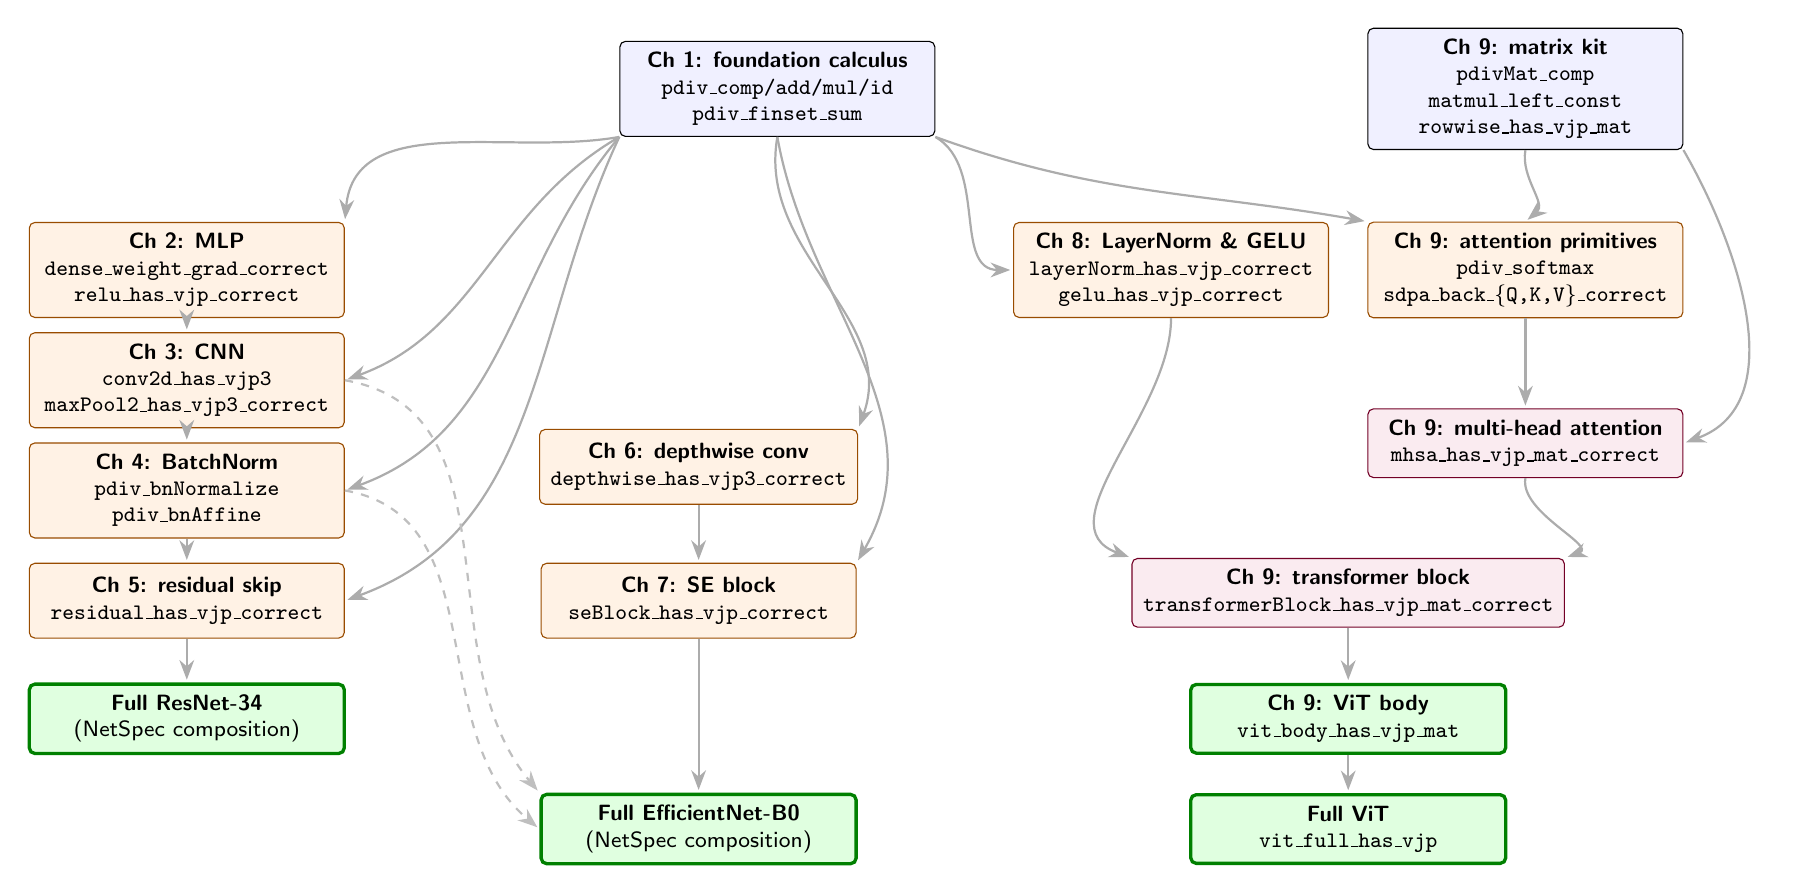
\begin{tikzpicture}[
  >={Stealth[length=2.5mm]},
  every node/.style={font=\sffamily\footnotesize},
  group/.style={
    draw, rounded corners=2pt, fill=blue!6,
    align=center, inner sep=4pt, minimum width=4.0cm, minimum height=1cm
  },
  primitive/.style={
    draw=orange!60!black, rounded corners=2pt, fill=orange!10,
    align=center, inner sep=4pt, minimum width=4.0cm, minimum height=0.95cm
  },
  composed/.style={
    draw=purple!60!black, rounded corners=2pt, fill=purple!8,
    align=center, inner sep=4pt, minimum width=4.0cm, minimum height=0.85cm
  },
  final/.style={
    draw=green!50!black, rounded corners=2pt, fill=green!12,
    align=center, inner sep=4pt, minimum width=4.0cm, minimum height=0.85cm,
    very thick
  },
  arr/.style={->, thick, gray!65, shorten >=1pt},
  shared/.style={->, thick, gray!50, dashed, shorten >=1pt}
]

% Top row: Ch 1
\node[group] (found) at (-1.5, 0) {
  \textbf{Ch~1: foundation calculus}\\
  \texttt{pdiv\_comp/add/mul/id} \\
  \texttt{pdiv\_finset\_sum}
};
\node[group] (matkit) at (8.0, 0) {
  \textbf{Ch~9: matrix kit} \\
  \texttt{pdivMat\_comp} \\
  \texttt{matmul\_left\_const} \\
  \texttt{rowwise\_has\_vjp\_mat}
};

% Left pillar: ResNet-34
\node[primitive] (mlp) at (-9.0, -2.3) {
  \textbf{Ch~2: MLP} \\
  \texttt{dense\_weight\_grad\_correct} \\
  \texttt{relu\_has\_vjp\_correct}
};
\node[primitive] (cnn) at (-9.0, -3.7) {
  \textbf{Ch~3: CNN} \\
  \texttt{conv2d\_has\_vjp3} \\
  \texttt{maxPool2\_has\_vjp3\_correct}
};
\node[primitive] (bn)  at (-9.0, -5.1) {
  \textbf{Ch~4: BatchNorm} \\
  \texttt{pdiv\_bnNormalize} \\
  \texttt{pdiv\_bnAffine}
};
\node[primitive] (res) at (-9.0, -6.5) {
  \textbf{Ch~5: residual skip} \\
  \texttt{residual\_has\_vjp\_correct}
};
\node[final] (r34) at (-9.0, -8.0) {
  \textbf{Full ResNet-34} \\
  (NetSpec composition)
};

% Middle pillar: EfficientNet (shifted south to clear shared-arrow lines)
\node[primitive] (dw) at (-2.5, -4.8) {
  \textbf{Ch~6: depthwise conv} \\
  \texttt{depthwise\_has\_vjp3\_correct}
};
\node[primitive] (se) at (-2.5, -6.5) {
  \textbf{Ch~7: SE block} \\
  \texttt{seBlock\_has\_vjp\_correct}
};
\node[final] (enet) at (-2.5, -9.4) {
  \textbf{Full EfficientNet-B0} \\
  (NetSpec composition)
};

% Right pillar: ViT
\node[primitive] (lngelu) at (3.5, -2.3) {
  \textbf{Ch~8: LayerNorm \& GELU} \\
  \texttt{layerNorm\_has\_vjp\_correct} \\
  \texttt{gelu\_has\_vjp\_correct}
};
\node[primitive] (attn) at (8.0, -2.3) {
  \textbf{Ch~9: attention primitives} \\
  \texttt{pdiv\_softmax} \\
  \texttt{sdpa\_back\_\{Q,K,V\}\_correct}
};
\node[composed] (mhsa) at (8.0, -4.5) {
  \textbf{Ch~9: multi-head attention} \\
  \texttt{mhsa\_has\_vjp\_mat\_correct}
};
\node[composed] (block) at (5.75, -6.4) {
  \textbf{Ch~9: transformer block} \\
  \texttt{transformerBlock\_has\_vjp\_mat\_correct}
};
\node[final] (body) at (5.75, -8.0) {
  \textbf{Ch~9: ViT body} \\
  \texttt{vit\_body\_has\_vjp\_mat}
};
\node[final] (vit) at (5.75, -9.4) {
  \textbf{Full ViT} \\
  \texttt{vit\_full\_has\_vjp}
};

% Foundation -> R34 primitives. Arrow to Ch 3 routes via cnn.east so it
% sweeps below Ch 2 instead of through it.
\draw[arr] (found.south west) to[out=-170, in=85] (mlp.north east);
\draw[arr] (found.south west) to[out=-150, in=20] (cnn.east);
\draw[arr] (found.south west) to[out=-130, in=20] (bn.east);
\draw[arr] (found.south west) to[out=-115, in=20] (res.east);
% Foundation -> ENet primitives
\draw[arr] (found.south) to[out=-100, in=70] (dw.north east);
\draw[arr] (found.south) to[out=-80, in=60] (se.north east);
% Foundation -> ViT primitives
\draw[arr] (found.south east) to[out=-30, in=180] (lngelu.west);
\draw[arr] (found.south east) to[out=-20, in=170] (attn.north west);
% Matrix kit -> ViT side
\draw[arr] (matkit.south) to[out=-100, in=40] (attn.north);
\draw[arr] (matkit.south east) to[out=-60, in=20] (mhsa.east);

% R34 down-flow
\draw[arr] (mlp) -- (cnn);
\draw[arr] (cnn) -- (bn);
\draw[arr] (bn)  -- (res);
\draw[arr] (res) -- (r34);

% ENet path
\draw[arr] (dw) -- (se);
\draw[arr] (se) -- (enet);
\draw[shared] (cnn.east) to[out=-10, in=130] (enet.north west);
\draw[shared] (bn.east)  to[out=-10, in=140] (enet.west);

% ViT down-flow
\draw[arr] (attn) -- (mhsa);
\draw[arr] (mhsa.south) to[out=-100, in=20] (block.north east);
\draw[arr] (lngelu.south) to[out=-90, in=160] (block.north west);
\draw[arr] (block) -- (body);
\draw[arr] (body)  -- (vit);
\end{tikzpicture}}
\caption{Three architecture spines, all the way down to Ch~1 foundation. ResNet-34 (left) needs only the foundation calculus and Chs~2--5 primitives. EfficientNet-B0 (middle) adds Ch~6's depthwise conv and Ch~7's SE block, and dashed arrows mark Chs~3 (CNN) and 4 (BN), shared with R34. ViT (right) is the only path that needs the matrix kit, and its longer chain runs through MHSA and the transformer block before bundling into the full ViT VJP. Every node is a Lean theorem.}
\label{fig:spines}
\end{figure}

\section{Proven: the math is right}

Two mechanisms make the deductive layer trustworthy: the proofs
themselves, and an independent re-check that the \emph{kernel}, not
just the elaborator, accepts them with no project axioms.

\subsection{Trust kernel}

The Verified VJP Proofs suite proves \textbf{70 VJP correctness
theorems}, one per layer, operator, and whole-network architecture,
each asserting backward \(= \sum_j \pdiv f\,x\,i\,j \cdot dy_j\), on
top of the foundation \(\pdiv\) calculus and the
differentiability/forward/witness machinery they rest on, plus the 41
architecture definitions in the bestiary --- and \textbf{zero project
axioms} anywhere in it. That last figure is the one that matters, because
it is the only one that cannot quietly grow. The axiom audit
(\texttt{tests/AuditAxioms.lean}) re-checks \emph{every} theorem in the
suite (the VJP contracts plus the forward-graph faithfulness, render,
cotangent-chain, backward-tie, and finite-precision results,
\S~\ref{sec:precision}) --- that file is the live count, quoted here
deliberately as a property rather than a number --- and every one closes
under the same three core axioms: \(\texttt{\#print axioms vit\_full\_has\_vjp}\) shows only
Lean core (\texttt{propext}, \texttt{Classical.choice},
\texttt{Quot.sound}), nothing project-level beneath those. (Earlier
drafts axiomatized shortcuts for the kinked operators, and every one has
since been proved or become a \texttt{noncomputable def} over the
canonical \(\fderiv\)-derived witness. The smooth-point caveats in
the chapters are all that remains of them.)

What type-checking alone cannot catch: prose narrating a different
formula than the theorem states (Lean only verifies its own statement),
and anything past the elaborator, which is what the next mechanism
and the empirical layer are for.

\subsection{Independent kernel re-check (comparator)}

\texttt{tests/comparator/} wires the project up to
\href{https://github.com/leanprover/comparator}{leanprover/comparator},
the Lean community's trustworthy-judge tool for projects that claim
zero project axioms. It runs 51 theorems (the foundation rules,
every chapter's headline Jacobian, the public
\texttt{*\_has\_vjp\_correct} wrappers, and three smooth-point
pointwise variants (\texttt{relu\_has\_vjp\_at\_correct},
\texttt{mlp\_has\_vjp\_at\_correct},
\texttt{maxPool2\_has\_vjp\_at3\_correct}) whose underlying
\texttt{.correct} field is a real proof rather than \texttt{rfl})
through Lean's kernel typechecker independently of the elaborator,
with an axiom-allowlist of exactly \(\{\texttt{propext},
\texttt{Quot.sound}, \texttt{Classical.choice}\}\). Any project
axiom in the transitive closure of any verified theorem would fail
the run.

This is what closes the gap between ``the elaborator accepted my
proofs'' (which \texttt{lake build} confirms) and ``the kernel
agrees, audited from a separate process'' (which comparator confirms).
The 51-theorem coverage is illustrative rather than exhaustive, since
the same recipe scales to any subset of the proof suite, and the
same allowlist applies because every theorem in the project closes
the same way.

\section{By construction: the code is the math}

\subsection{Verified code generation}
\label{sec:verified_codegen}

The proofs above answer whether the \emph{mathematics} is right, meaning the
hand-derived VJPs, their proofs, and the elaborator that accepted them. They
say nothing about a different gap. The GPU never runs the Lean functions. It
runs a block of emitted \texttt{stablehlo} that the lowerer compiles once per
training program. A code generator can be handed a correct proof and still
emit an operation that contracts the wrong axis, transposes backwards, or
silently drops a term, and the only thing traditionally linking the proof
to the emitted string is a code comment. The ``MLIR: \emph{operator}''
section in each chapter closes that gap for one operator, and this section
describes the machinery they share.

\medskip\noindent\textbf{Three pieces.} The link from a proof to the GPU is
built from three components:

\begin{itemize}
  \item \textbf{Denoted IR and a bridge theorem.} The emitted backward (and
    forward) is not a string but a Lean datatype, a small abstract syntax
    tree (\texttt{Back}, \texttt{Fwd}, \texttt{Back3}), carrying a
    denotation $[\![\cdot]\!]$ valued in the proofs' own \texttt{Vec} and
    \texttt{Tensor3} types. A \emph{bridge theorem} then proves that this
    denotation equals the proven derivative: $[\![\,\text{emitted
    graph}\,]\!] = (\text{proven VJP}).\mathrm{backward}$. Examples are
    \texttt{conv\_back\_bridge}, \texttt{bn\_back\_bridge}, and
    \texttt{relu\_back\_bridge}, and each closes under the same three axioms
    as the rest of the project.
  \item \textbf{A computable printer.} A small printer walks that same IR and
    emits one \texttt{stablehlo} operation per node, so
    \texttt{dotGeneral}\,$W$ becomes \texttt{stablehlo.dot\_general}, a
    \texttt{selectPos} node becomes \texttt{compare GT 0} plus
    \texttt{select}, and so on. The emitted text \emph{is} the printout of
    the IR, by construction.
  \item \textbf{An execution oracle.} A Python harness regenerates the
    \texttt{.mlir} from the printer, compiles it with IREE for both the
    \texttt{llvm-cpu} and \texttt{rocm} backends, runs it, and diffs the
    result against an independent NumPy reference. The CPU run is the
    correctness gate, and the GPU run (ROCm on a Radeon RX 7900 XTX, gfx1100)
    confirms the proof-backed graph also executes on real hardware, matching
    the reference to roughly $10^{-6}$.
\end{itemize}

\medskip\noindent\textbf{Proven versus trusted.} The resulting claim is exact
and bounded:
\begin{itemize}
  \item \emph{Proven} (Lean, three axioms): the IR's denotation equals the
    proven derivative.
  \item \emph{By construction}: the emitted StableHLO is the rendering of
    exactly that IR.
  \item \emph{Trusted} (validated numerically, not proven): that the
    StableHLO \emph{text} faithfully denotes $[\![\cdot]\!]$. Its
    \emph{syntactic} half is now partly closed, because the emitted text lexes
    and parses back to the proven op-graph (\texttt{StableHLOLex.lean},
    \texttt{StableHLOParse.lean}). That leaves three things trusted: a formal
    StableHLO \emph{semantics}, which does not yet exist, that the lowerer
    compiles the text correctly, and that the hardware's rounding
    approximates $\mathbb{R}$ within the modelled unit roundoff. The last of those is now a conditional theorem validated on
    real silicon (\S~\ref{sec:precision}) rather than a bare assumption.
\end{itemize}
So the gradient the GPU computes is, by a machine-checked theorem, the
network's exact reverse-mode derivative over $\mathbb{R}$, up to one
printer, one lowerer, and floating point. Where a conventional generator leaves
thousands of lines of string-building linked to the proof by nothing at all,
the unproven surface here is a single printer, tested end to end.

\medskip\noindent\textbf{Why it is tractable.} The reason a deep ResNet or a
transformer block comes under this scheme as a focused engineering build,
rather than a research project, is the order things were proved in. The VJP
library is \emph{per-operator and generic}, proved once over abstract
dimensions and before any code generation existed, and the whole-network VJPs
compose those per-operator lemmas through the chain rule. Code generation
therefore carries \emph{no new proof obligation}: every architecture's
operators were proven once, and the emitter reuses them, adding only the
printer and the numerical check. Build the mathematical foundation
per-operator and generic, and the code generation becomes mechanical.

\medskip\noindent\textbf{From operators to whole training steps.} The
per-operator bridge is the demonstration, and the verified trainers run the
full construction. Each reads a single committed \texttt{.mlir} holding its
entire training step, forward through backward through the parameter update,
and that file is the printout of one graph whose denotation a faithfulness theorem
proves equal to the certified loss-descent step, output by output. A companion
\emph{tie} theorem per network (\texttt{<net>\_net\_tied\_certified}) then
closes the gap a per-output bridge leaves open: the cotangent each parameter
update consumes is the one the network's \emph{own} backward pass delivers at
that site, threaded through the real forward activations, so each update is
one composed equation rooted at the proven forward rather than a quantifier
over a free cotangent. All twelve chapter networks are tied this way, from the MNIST
linear classifier to depth-12 ViT-Tiny, and each deep net's rendered
block-backward is pinned to that block's certified VJP
(\texttt{vitBlockBackPR\_eq\_transformerBlock\_vjp} and its peers). The axiom
audit re-derives every tie under the same three axioms, and CI prints a green
cell for a network only when its tie capstone is in that closure, so the
scorecard cannot claim more than the kernel checked. What stays trusted is
exactly what the per-operator story already trusted, now carried across the
whole step: the one printer, and that each emitted operation's text denotes
what $[\![\cdot]\!]$ says it does.

\medskip\noindent\textbf{The one conditional.} For the smooth operators the
bridge is unconditional, holding at every input, and those are BatchNorm and
LayerNorm (given $\varepsilon > 0$), GELU, swish, sigmoid, softmax, and
attention. For the kinked operators, which are ReLU, ReLU6 and max-pool, it
holds only at a \emph{smooth point}, where no pre-activation sits exactly on
the kink (zero for ReLU, $0$ or $6$ for ReLU6, an argmax tie for max-pool).
The equality is permitted to fail precisely on that measure-zero set, and
nowhere else. That set is the one irreducible boundary the smooth-point caveats in
the chapter sections refer to.

\subsection{Inside a bridge theorem}
\label{sec:inside_bridge}

The ``denoted IR and a bridge theorem'' above is worth seeing concretely,
because it is the step that does the real work, the place where a string of
emitted code becomes a proposition Lean can check. Take the backward pass. It
is represented not as text but as a value of an inductive type, a small
abstract syntax tree whose constructors are exactly the StableHLO operations a
backward uses:

\begin{verbatim}
inductive Back (inp : Nat) : Nat -> Type where
  | cotangent  : Back inp inp            -- the input dy
  | dotGeneral (A : Mat m n) : Back inp n -> Back inp m   -- matmul
  | selectPos  (x : Vec n)   : Back inp n -> Back inp n   -- ReLU mask
  -- plus scale, sub, add, sumBroadcast, scaleConst (BN, residuals)
\end{verbatim}

\noindent A \texttt{Back} value is a closed description of one backward graph.
The dense backward, for instance, is just \texttt{dotGeneral W cotangent},
which feeds the incoming cotangent into a single matrix multiply. Two functions are
defined on this type, and \emph{everything} rests on the gap between them
being closed by a theorem.

\medskip\noindent\textbf{The denotation.} The first function,
\texttt{Back.denote}, interprets a graph into the proofs' own \texttt{Vec}
type, saying what the graph \emph{means} mathematically:
\[
  [\![\texttt{cotangent}]\!]\,dy = dy, \qquad
  [\![\texttt{dotGeneral}\,A\,e]\!]\,dy
    = \texttt{Mat.mulVec}\,A\,([\![e]\!]\,dy),
\]
\[
  [\![\texttt{selectPos}\,x\,e]\!]\,dy
    = \bigl(i \mapsto \text{if } x_i > 0
      \text{ then } [\![e]\!]\,dy\,i \text{ else } 0\bigr),
\]
and likewise for the remaining constructors (\texttt{scale}, \texttt{sub},
\texttt{sumBroadcast}, \texttt{scaleConst} and \texttt{add}), which are the
pieces that assemble BatchNorm's three-term backward and the residual fan-in.
So a \texttt{Back} value denotes a concrete $\texttt{Vec} \to \texttt{Vec}$
function, living in the same world as the VJP theorems.

\medskip\noindent\textbf{The bridge, as an equation.} A bridge theorem states
that this denotation equals the proven derivative. For the dense layer:
\[
  \texttt{dense\_back\_bridge}:\quad
  [\![\texttt{emitDenseBack}\,W]\!]\,dy
  = (\texttt{dense\_has\_vjp}\,W\,b).\mathrm{backward}\,x\,dy.
\]
Its proof is one word, \texttt{rfl}: both sides reduce to the \emph{same}
term, \texttt{Mat.mulVec}\,$W\,dy$, so the denotation of the emitted graph and
the proven backward are definitionally identical. That base case pins the
plumbing. The ReLU bridge is the first with real content:
\[
  \texttt{relu\_back\_bridge}\ \ (h_{\text{smooth}} : \forall k,\ x_k \ne 0):
  \quad
  [\![\texttt{emitReluBack}\,x]\!]\,dy\,i
  = (\texttt{relu\_has\_vjp}\,n).\mathrm{backward}\,x\,dy\,i.
\]
The proof unfolds the denotation to $\text{if } x_i > 0 \text{ then } dy_i
\text{ else } 0$ and shows it equals the canonical ReLU subgradient, but
\emph{only} under the hypothesis $h_{\text{smooth}}$ that no coordinate sits
on the kink. That hypothesis is not a technicality. It names exactly the
measure-zero set where the emitted \texttt{compare GT 0} disagrees with the
true derivative, and the theorem is written to permit failure precisely there
and nowhere else. The convolution bridge of Chapter~\ref{chap:cnn} is the same
shape with a harder proof: \texttt{convBackDenote} unfolds to a forward
\texttt{conv2d} of the reversed-and-transposed kernel, discharged by expansion
at the concrete tensor shape.

\medskip\noindent\textbf{Composing the per-operator bridges.} Whole-network
backwards are assembled by substitution. \texttt{Back.subst} plugs one graph
into another's \texttt{cotangent} leaf, and a chain-rule lemma proves the
denotation composes:
\[
  \texttt{denote\_subst}:\quad
  [\![\,e[g/\texttt{cotangent}]\,]\!]\,dz
  = [\![e]\!]\,([\![g]\!]\,dz),
\]
proved by induction over the graph, the IR-level analogue of the
\texttt{vjp\_comp} that builds whole-network VJPs from per-layer ones. So the
per-operator bridges compose into a whole-network bridge the same way the VJP
theorems compose into a whole-network VJP: the MLP's
\texttt{mlp\_whole\_bridge} is this one substitution, chaining its five
per-operator bridges.

\medskip\noindent\textbf{Why the datatype is the point.} The \texttt{Back}
value is the pivot between two arrows. The printer walks it and emits one
\texttt{stablehlo} operation per constructor (\texttt{dotGeneral} $\mapsto$
\texttt{stablehlo.dot\_general}, and \texttt{selectPos} $\mapsto$
\texttt{compare GT 0} plus \texttt{select}), and that arrow is the trusted
one, producing the text in each chapter's listing. The denotation interprets
the same value into the proofs' \texttt{Vec} type, and the bridge proves
\emph{that} equals the derivative, so that arrow is machine-checked. Because both arrows start from
one concrete datatype rather than from a string, ``the emitted code computes
the proven gradient'' is a theorem about a value, not a hope about a comment.

\section{Cross-checked}

Neither lowerer can itself be proven, and GPU transcendentals have no
IEEE specification, so the last stretch from proven math to executed
kernel is covered by independent oracles that must agree before the
hardware is believed. Each watches a different failure mode.

\medskip\noindent\textbf{The property that makes this work is that the two
sides do not share a compiler.} The Lean-side pipeline of the oracles below
lowers through IREE, and the reference pipeline is JAX, which lowers through XLA.
Different code generation, different runtime, different kernels, and different
authors. Agreement between them is evidence precisely because a bug would have
to occur twice, in the same direction, in two unrelated compilers. This is
IREE's real job in the project, and it is not the one the runtime-size
comparison in Appendix~\ref{app:getting_started} might suggest. IREE is not
kept because it is small. It is kept because it is not XLA.

\subsection{Finite-difference gradient checks}

The script \texttt{LeanMlir/Proofs/check\_jacobians.py} runs 30
finite-difference gradient checks. For each, it perturbs the input by
\(\varepsilon\), compares the claimed VJP against the centered
difference
\((f(x + \varepsilon) - f(x - \varepsilon)) / 2\varepsilon\), and
asserts agreement within tolerance (typical max-error
\(\sim 10^{-11}\) at \(\varepsilon = 10^{-5}\) in float64).

Every FD check is a belt-and-suspenders pass over a
\emph{proved} Jacobian theorem.
The proofs already establish that each formula equals
\(\fderiv\) at the relevant points, and the FD checks confirm
the formulas-as-written agree numerically with what the function
actually does. Coverage spans every closed-form Jacobian we use
downstream: \(\pdiv\_\texttt{dense}\) and its weight/bias
companions, \(\pdiv\_\texttt{relu}\) (at smooth points),
softmax cross-entropy, all four BN pieces
(\texttt{bnNormalize}, \texttt{bnCentered},
\texttt{bnIstdBroadcast}, \texttt{bnAffine}), the conv2d and
depthwise input/weight/bias VJPs, the maxPool2 input VJP, and the
softmax Jacobian. It also covers the three single-head SDPA Q/K/V
backwards, GELU, the bundled multi-head SDPA reduction (per-head
\texttt{sdpa\_back} stacked over the head axis), the patch-embed
input VJP, the full-network MLP composition, and bestiary
spot-checks (bilinear upsample, channel concat, per-pixel
softmax cross-entropy, U-Net skip plumbing).

What the FD pass catches that the symbolic proof can't: typos
between the proof and the prose that uses the same Jacobian.
If a chapter narrates one formula but the Lean theorem states
another, the proof still type-checks (Lean only verifies its
own statement), but the FD test runs against the formula the
prose published and would diverge.

FD is cheap, easy to reason about, and tight enough for
spot-checking formulas, but it can't probe what the
\emph{compiled} code actually computes on the GPU, only
what the formula says in Python, and it struggles at
non-smooth points where the limit definition breaks down. For
those gaps and for end-to-end pipeline verification, the next oracle takes over.

\subsection{The JAX parallel pipeline}
\label{sec:jax_pipeline}

A separate Lean \(\to\) JAX \(\to\) XLA pipeline
(\texttt{jax/Jax/Codegen.lean}, \(\sim 1100\) lines) produces an
idiomatic JAX training script from the same \texttt{NetSpec} the
Lean \(\to\) StableHLO MLIR pipeline consumes. XLA is the compiler
JAX uses to produce GPU code, the same backend that powers
TensorFlow and other frameworks. For this comparison the Lean side
is lowered by IREE, so the two stacks are independent end to end,
with different code generation, different runtime and different
kernels, and that is why agreement between them is a meaningful
cross-check. Running both from identical initial parameters on
identical batches gives us a pair of trace files, one per stack,
that should agree modulo float32 rounding if both pipelines compute
the same math.

The agreement is very tight. For the MNIST MLP, step-1 losses agree
to \(\sim 2 \times 10^{-7}\), which is float32 ULP, across the
JAX-CPU-vs-IREE-ROCm comparison, and the IREE output is
\textbf{bit-identical across AMD and NVIDIA hardware} at step 1.
For the MNIST CNN with batch norm, step-1 agrees to
\(\sim 10^{-4}\), looser because variance reductions over
\(\sim 100\)k-element tensors amplify cross-compiler reduction-tree
differences. Both pipelines do correct math, they just sum it
in different orders. Full results are committed to the repo as
reproducible JSON-Lines traces, in
\texttt{traces/CROSS\_BACKEND\_RESULTS.md}.

\medskip\noindent\textbf{One asymmetry, stated plainly.} The trainers in this
book default to XLA, while the oracles above lower the Lean side through IREE.
That is deliberate, because an oracle that shared a compiler with its own
reference would not be checking the compiler at all. The consequence is worth
being clear about: it is IREE's translation of the proven text that these
oracles exercise directly, so the default training path's lowering carries less
of this particular kind of evidence than the path the oracles run. Every other
layer is unaffected, since the proofs, the bridge theorems and the
rounding budgets are statements about the graph rather than about any
compiler, and both lowerers consume the identical proven StableHLO.

Layered on top of the end-to-end trace diff is a per-axiom
differential test in \texttt{tests/vjp\_oracle/}, which compares
each Lean-proved backward pass against JAX's
\texttt{value\_and\_grad} autodiff on a minimal one-step training
run. Nine cases each agree with JAX autodiff at 1--2 ULP of step-2 loss,
and they are dense, dense+ReLU, conv, conv+BN, conv+maxPool,
residual, depthwise, SE and attention. Any future hand-derived VJP added to
the Lean proof base can be validated by a one-step comparison
against JAX, catching algebraic errors that FD would miss (sign
flips, wrong contraction axis, swapped indices).

\subsection{The execution oracle and the margin probe}

Two further watchers close the loop. The \textbf{IREE-versus-NumPy
oracle} (\S~\ref{sec:verified_codegen}) regenerates every committed
\texttt{.mlir} from the printer, compiles it for CPU and GPU, and diffs
the result against an independent NumPy reference, which is the one check
that reaches past the proofs to IREE's lowering itself. And the
\textbf{margin probe} (\texttt{scripts/margin\_probe.py}) re-runs a real
training trajectory in coupled \texttt{f32}/\texttt{f64} and checks that
the run stays inside the float theorems' hypotheses, with no flipped ReLU
mask and no logit drift past \(\delta\) (\S~\ref{sec:precision}). It is
what keeps the conditional theorems honest about actual training rather
than hypothetical nets.

\bigskip

Each kind fails differently, and overlaying them is the guarantee. A
deductive proof is blind to a miscompile, an empirical diff is blind to a
measure-zero kink, and a faithful bridge is blind to a wrong formula it
renders perfectly. Verified code generation straddles two
of the kinds: its bridge is structural, its oracle empirical. The
finite-precision theorem layer, next, straddles the other pair: its
budgets are deductive, its interface constants (\(u\), \(e_{\exp}\),
\(\delta\)) empirical.

\section{Finite precision}
\label{sec:precision}

Every theorem in this book is over exact reals, and the GPU computes in
finite precision. Until recently that gap lived entirely in the empirical
layer, where the oracles agree to 1--2 ULP. It is now a theorem layer, and
it has two halves of different reach. Keeping them apart is the honest
part --- as is keeping the layer's \emph{generality} apart from its
\emph{usefulness}, which \S~\ref{par:precision_reach} below returns to.
The \emph{closeness} half
(\(|\,\text{float op} - \text{real op}\,| \le\) budget) is
architecture-complete: \texttt{FloatBridge.lean} and the per-net
\texttt{*FloatBridge} files budget every operator of every network, forward
and backward, from the MNIST linear classifier to ViT-Tiny, and (by the
composition theorem below) these per-operator budgets fold into a
\emph{depth-linear whole-network} certificate that stays below the logit scale
on eight of the nine committed renders. The
\emph{descent} half (a rounded step provably \emph{decreases the loss})
closes only for the shallow nets
(\texttt{SgdDescent\{Linear,Mlp,Cnn,Cifar\}.lean}). The way the chain avoids
new axioms is the part worth explaining.

\paragraph{The model is a hypothesis.}
A \texttt{FloatModel} is \emph{any} rounding operator \(\mathrm{rnd}\)
with relative error \(u\): \(|\mathrm{rnd}(x) - x| \le u\,|x|\).
Binary32 round-to-nearest satisfies this with \(u = 2^{-24}\) on the
normal range (the subnormal range is characterized separately in
\texttt{FloatSubnormalBridge.lean}, where the normalized blocks provably stay
normal and the residual underflow floor is proven negligible at
\(\le 2^{-86}\)). The exact-arithmetic model
(\(\mathrm{rnd} = \mathrm{id}\), \(u = 0\)) shows the interface is
inhabited and collapses every budget to zero. Nothing about IEEE-754 is
postulated, and the theorems are conditional on the standard model, the
same way the ReLU theorems are conditional on being off the kink, and
the axiom audit is untouched. Two further design choices are forced by
the hardware: the dot-product budgets are stated in the classical
compounded form valid for \emph{every} summation association, because
IREE tiles and reorders reductions freely (the price is a fan-in factor
\(n\cdot u\), and the tree-reduction bound below recovers
\(\log_2 n\cdot u\) under a named balance hypothesis). And \(\exp\) enters
as a hypothesis (\(|\widehat{\exp}(t) - e^t| \le e_{\exp}\, e^t\))
because GPU transcendentals have no IEEE specification.
\(e_{\exp}\) is precisely the constant the VJP oracle
(\S~\ref{sec:jax_pipeline}) measures, so the deductive and empirical
layers meet at a named interface instead of a hand-wave.

\paragraph{How far the model reaches, and where it stops being useful.}
\label{par:precision_reach}
Because \(u\) is a parameter, nothing in the chain is
\texttt{float32}-specific. \texttt{Binary32Instance.lean} constructs the
rounding operator as round-to-nearest on the \(p\)-bit-significand grid
and instantiates it twice: \texttt{binary32} at \(p = 23\),
\(u_{32} = 2^{-24}\), and \texttt{fp8E4M3} at \(p = 3\),
\(u_{\mathrm{e4m3}} = 2^{-4}\). Every whole-network bridge quantifies over
\texttt{(M : FloatModel)}, so ResNet-34's certificate is not a statement
about binary32 that happens to be proved --- it is a statement about
\emph{any} rounding model, of which binary32 is one instance.

\medskip\noindent That generality is free. Usefulness is not, and the two
should not be confused. The dot-product budget carries the classical
fan-in factor \((1+u)^{n+1} - 1\), which goes vacuous once \(n\,u\)
approaches 1 --- a wall at \(n \approx 1/u\). At \(u_{32}\) that wall sits
near \(1.7 \times 10^{7}\) and no layer in this book comes close. At pure
bf16 (\(u = 2^{-8}\)) it sits at \(n \approx 256\), and ResNet-34's
\(3\times3\) convolution at 512 channels has fan-in 4608. The budget is
still true there. It is also worthless there.

\medskip\noindent Which is why the low-precision result is stated
\emph{mixed} rather than pure. \texttt{dotMixed} rounds the operands
through a leaf model \(L\) (bf16 \(2^{-8}\), or fp8-E4M3 \(2^{-4}\)) and
accumulates through \(M\) at \(u_{\mathrm{acc}}\), which is the shape the
hardware actually runs: low-precision inputs, fp32 accumulator.
\texttt{dot\_close\_mixed} then splits the error in two, and the split is
the whole point --- the leaf precision contributes a \emph{flat}
\((2u_{\mathrm{leaf}} + u_{\mathrm{leaf}}^2)\sum|x_i y_i|\) term that is
\textbf{not} fan-in amplified, while the amplification rides entirely on
\(u_{\mathrm{acc}}\). The wall stays at \(1/u_{\mathrm{acc}}\) no matter
how coarse the leaf is. That is exactly why bf16-mixed is non-vacuous
where pure bf16 is not, and it is carried to convolution and depthwise
convolution in \texttt{ConvMixedFloatBridge.lean},
\texttt{DepthwiseMixedFloatBridge.lean} and
\texttt{ConvMixedComposeBridge.lean}, with the emitted low-precision
graphs tied back to the intended algorithm in
\texttt{Bf16FaithfulPoC.lean} and \texttt{E4M3FaithfulPoC.lean}.

\medskip\noindent So the honest summary is three sentences, not one. The
theorems are over \(\mathbb{R}\). The budgets are over an arbitrary
rounding model, so binary32, bf16-mixed and fp8-E4M3 are instances rather
than separate theories. And the numbers those budgets produce are worth
having at fp32 accumulate, worth having at a low-precision leaf over an
fp32 accumulator, and not worth having at pure low precision --- which is
a fact about the arithmetic, not a gap in the proofs.

\paragraph{The chain.} Four links, each in the three-axiom audit.
\emph{Forward}: \texttt{mlp\_float\_close\_uniform} budgets the
rounded \(784{\to}512{\to}512{\to}10\) forward against the exact
one, from coordinatewise magnitude bounds alone. \emph{Backward}:
\texttt{mlp\_\{w2,w1,w0,b2,b1,b0\}\_step\_float\_close} budget
every rounded SGD parameter entry against \(\theta -
\mathrm{lr}\cdot(a_i c_j)\), entry for entry, and the
\texttt{emitWeightGrad} quantities the render closes
(\S~\ref{sec:verified_codegen}) prove equal to the
\(\pdiv\)-Jacobian contractions, so the float step chains to the
proven gradient. \emph{The loss head}:
\texttt{softmax\_ce\_cot\_close} budgets the rounded
softmax-minus-onehot cotangent against the certified
\(\partial(\mathrm{crossEntropy})/\partial(\mathrm{logits})\).
\emph{Descent}: \texttt{sgd\_descends} proves an \(\eta\)-accurate
gradient step still \emph{decreases the loss}, and
\texttt{linear\_sgd\_descends} discharges its smoothness hypothesis with
the explicit constant \(2a^2/(1-2aD)\), with no Hessian, because the softmax
ratio sandwich that powers the float budgets turns out to be the Lipschitz
engine too. With the float budget \emph{fused in}, so that the step's
\(\eta\) is the \emph{proven} binary32 gradient accuracy rather than an
assumed parameter, this closes end-to-end for the linear classifier
(\texttt{linear\_float\_sgd\_descends}), the entire MLP
(\texttt{mlp\_\{output,hidden,input\}\_float\_sgd\_descends}), and the
entire Chapter-3 CNN, both conv weights and biases
(\texttt{cnn\_conv\{1,2\}\_float\_sgd\_descends}). The \(\mathbb{R}\)-side
argument reaches one layer further:
\texttt{cifar8\_lastConv\_sgd\_descends} is the first non-MNIST descent. It is
CIFAR-8's last conv, proved as an \emph{instance} of the CNN lemma at its
frozen earlier features, and that framing is exactly why it stops there.
The admissible \(\mathrm{lr}\) is a product of per-layer operator-norm
factors, so each added layer shrinks it geometrically. Full-depth CIFAR and
all five deep nets stay closeness-only, by design, not for want of effort.

\paragraph{The kink.}
Over \(\mathbb{R}\), ReLU forced the hypotheses \(x_k \ne 0\). In
float the same op inverts its role twice. The forward mask is
\emph{exact}, since compare-and-select rounds nothing, so the op that
causes all the \(\mathbb{R}\)-side conditions is the free op here.
But the backward mask reads the \emph{rounded} pre-activation, so the
hypotheses return with a number in them, \(\mathit{ez} < |z_i|\), meaning
the accumulated rounding error must not flip a sign
(\texttt{reluMask\_close}). A qualitative side condition became a
checkable margin.

\paragraph{The naive whole-network bound is vacuous.}
Budgeting each operator is one thing. Combining those budgets into a bound on
the \emph{whole} network is another. The obvious way (\texttt{FloatClose.comp})
assumes every layer amplifies the error it inherits by that layer's
\emph{worst possible} factor, then multiplies those factors down the depth. So
the bound grows like \((\text{gain})^{\text{depth}}\) and blows up to
\(2.7\cdot 10^{60}\) on MobileNetV2 and \(\sim\!10^{364}\) on ViT-Tiny, while
the drift the GPU actually produces stays near \(10^{-5}\). Past a handful of
layers, that bound says nothing at all.

\paragraph{The adjoint chain: add, don't multiply.}
The real error behaves differently. Each layer's \emph{own} rounding is
amplified just once, by how much the \emph{rest} of the network magnifies a
small change made at that point, and those contributions \emph{add} instead
of multiplying. \texttt{chain\_adjointClose} (\texttt{AdjointChainBridge.lean})
proves exactly this: the whole-network error is at most \(\sum_i H_i\,b_i\),
where \(b_i\) is layer \(i\)'s fresh rounding budget (its per-operator bound,
before anything is inherited) and \(H_i\) is its \emph{tail gain}, meaning how
much a perturbation at layer \(i\) is stretched by all the layers after it. The proof
is a single induction, exact (nothing is linearized), and because each \(b_i\)
is amplified only once, the total grows roughly \emph{linearly} with depth
rather than exponentially. It can never lose to the naive bound: plug in
worst-case tail gains and you recover the old bound exactly, so any honest
estimate of \(H_i\) only helps. And an honest estimate is cheap, since one
backward pass reads the \(H_i\) off the network's own trajectory. They enter the theorem
as named hypotheses carrying their measured values, on the same footing as the
\(\exp\) constant (\S~\ref{sec:jax_pipeline}), never an axiom.

\paragraph{A certificate below the logit scale.}
Two refinements make the bound small in practice. Cut the chain at \emph{every}
operator, giving each convolution, normalization and dense its own link, with
residual connections carried alongside (\texttt{chain2\_adjointClose}), and
no worst-case products survive anywhere. And note that a sum of \(n\) terms
costs a factor \((1{+}u)^{n}\) only if the hardware adds them in the worst
order. IREE adds them in a balanced tree, which costs
\((1{+}u)^{\lceil\log_2 n\rceil}\) instead (\texttt{tree\_close},
\texttt{TreeReduceBridge.lean}), a factor we name and check empirically
rather than assume, and the one that finally tames the widest reductions
(fan-in \(6272\), or \(n = 301056\) in ConvNeXt's LayerNorm). The result is the
first whole-network float certificate that means something on networks this
deep: the bound lands \emph{below the logit scale} on eight of the nine
committed renders, quoted here as budget against that net's own logit scale
--- MNIST-MLP \(0.8/21\), MNIST-CNN \(0.015/0.64\), CIFAR-8 \(2.6/4.6\),
MobileNetV2 \(0.30/0.99\), ResNet-34 \(0.17/3.40\), ViT-Tiny \(0.57/4.33\),
EfficientNet-B0 \(0.096/0.94\), ConvNeXt-T \(0.80/2.94\). The ninth,
CIFAR-8-BN, is the one that does not close: \(3.4\) against a logit scale of
\(3.2\), or \(1.1\times\) over. It is quoted rather than dropped because it is
the honest edge of the method --- a per-example per-channel BatchNorm at
fan-in \(1024\) is the widest reduction in the set, and the residual is a
single tail gain of \(1313\) through \texttt{bn1}. Every other net clears by
between \(3\times\) and \(26\times\). And it is a statement about the \emph{decision}, not just
the numbers: \texttt{cifar8\_chain\_argmaxSafe} proves that whenever the exact
network's margin beats twice the budget, binary32 rounding cannot change which
class it predicts.

\paragraph{Measured against proven.}
The numeric capstones are instantiated at the \emph{trained} magnitudes
of a real 12-epoch, 97.8\% GPU run (\(|W| \le 3/5\), covering the
measured \(0.52\), and He initialization already exceeds prettier bounds
in its tails). An \texttt{f32}/\texttt{f64} twin of that run
(\texttt{scripts/margin\_probe.py}, per-step coupled to match the
single-step theorems) measures what the theorems bound:

\begin{center}
\begin{tabular}{lll}
quantity & worst-case theorem & measured \\
\hline
logit drift & \(\le 5100\) \;(\texttt{mnist\_mlp\_float\_budget}) & \(1.6\cdot 10^{-5}\) \\
cotangent & \(\le 21/1000\) \;(\texttt{mnist\_cot\_budget}) & \(2.2\cdot 10^{-6}\) \\
\(W_2\) SGD step & \(\le 5/4\) \;(\texttt{mnist\_w2\_step\_float\_budget}) & \(7.5\cdot 10^{-9}\) \\
ReLU mask flips & \(0\) under margins & \(\mathbf{0}\,/\,29.5\mathrm{M}\) \\
\end{tabular}
\end{center}

The worst-case bounds hold
with up to \(10^{8}\) to spare because worst-case composition
compounds magnitude bounds the way no real activation pattern does,
and that gap is exactly what the adjoint chain closes: its measured tail
gains are the a-posteriori certificate past toy depth, now a theorem
(\texttt{chain\_adjointClose}) rather than an asserted argument. The
whole-net budget was re-measured at the \emph{trained} weights of five real
checkpoints (ResNet-34, MobileNetV2, EfficientNet-B0, ViT-Tiny and
ConvNeXt-T), and it holds on every one, with the telling twist that it
\emph{tightens} where training removes a pathological initialization (ViT's
zero-init class token, MobileNetV2's He-init stem gain) and only loosens
slightly on clean-init nets: the certificate is demonstrably a property of
the deployed network, not an artifact of the initialization. And the
flip count is zero across 29.5 million measured pre-activations. The
margin hypotheses are not a technicality the proofs hide behind. They
are what training actually looks like.

\chapter*{Acknowledgments}
\addcontentsline{toc}{chapter}{Acknowledgments}

Thanks to \textbf{Tomáš Skřivan}, whose
\href{https://lecopivo.github.io/scientific-computing-lean/Working-with-Arrays/Tensor-Operations/}{Scientific Computing in Lean}
bootstrapped this project's first MNIST trainer.

\noindent Thanks to \textbf{Monica Omar} on
\href{https://leanprover.zulipchat.com/}{Lean Zulip}, who closed
the 6-level \texttt{Finset.sum} commutation in the Conv2D VJP
proof.

\noindent Thanks to \textbf{Franz Huschenbeth} on
\href{https://leanprover.zulipchat.com/}{Lean Zulip} for reviewing
early drafts and suggesting the comparator approach used in
Appendix~\ref{app:verification}.

% =====================================================================
%  Colophon — closing chapter on authorship in the AI age. SKELETON:
%  the live text below is just the honest acknowledgment; the four
%  argument-threads are stubbed as comments to develop into the essay.
%  (Title stays "Colophon" — matches the book's manuscript/auctoritas
%  theme; could carry a Steinbeck "hooptedoodle" epigraph if wanted.)
% =====================================================================
\chapter*{Colophon}
\addcontentsline{toc}{chapter}{Colophon}

\emph{Here ends the book.}

It was written with the help of a machine. The text was written in
LaTeX. The proofs in it were checked by Lean's kernel. The prose, the
code, and the path to both were drafted in collaboration with Qwen and
Claude, which served by turns as three things: as \emph{scribe}, taking
dictation, as \emph{compilator}, searching and assembling, and as
\emph{commentator}, proposing framings I kept or discarded. I remained
the author in the one sense that outlives the machine: I am the one
answerable for what is here.

% --- TODO: the four threads, to develop into the essay ---
% (1) Picasso / cheap paint: critics talk Form and Meaning; the painter
%     asks where to buy cheap turpentine. The maker uses the tool; the
%     universal-truths anxiety is the critic's hobby, not the maker's.
% (2) Stochastic parrots cut both ways: humans pattern-match from their
%     training too, and on plain literacy the machine already clears much
%     of the species. The dismissal, taken seriously, indicts the accuser.
% (3) The centaur: a human plus a machine exceeds any unaided human;
%     refusing the tool is choosing to be weaker on purpose.
% (4) No book larger than the deposit: nothing drawn from the corpus
%     exceeds the corpus; the maker's office was never bigness, it is
%     selection and answerability.  [confirm intended sense]
% Tension is the point: the centaur brags, the deposit humbles — a
% colophon can hold both where a thesis can't.

\noindent Where the words are clumsy or wrong, blame not the compiler nor
the models but the author, not the tools.

\end{document}